
\documentclass[
%	draftmark = true,
	colors = true,
%	colors = false,
	coverpage = coverpage-em.tex,
%	coverpage = coverpage-em.pdf,
	fontsetup = font-setup-open-em.tex,
%	fontsetup = font-setup-HEP-em.tex,
	titlesetup = titles-setup-em.tex
]{AJbook}

\usepackage{mathrsfs}
\usepackage{stmaryrd} \SetSymbolFont{stmry}{bold}{U}{stmry}{m}{n}	% 避免警告 (stmryd 不含粗体故)
\usepackage{array}
\usepackage{makecell}	% 便于制表
\usepackage{tikz-cd}  % 使用 TikZ 绘图
\usetikzlibrary{positioning, patterns, calc, matrix, shapes.arrows, shapes.symbols}
\usepackage{braids}
\usepackage{tqft}
\usepackage{ytableau}

% PGF plots 用于封面绘制
\usepackage{pgfplots}
\pgfplotsset{compat=newest}

% 设置章节深度
%\setcounter{secnumdepth}{1}

% 必要时仅引入部分档案
% \includeonly{}

\usepackage{booktabs}

\usepackage{myarrows}				% 使用自定义的可伸缩箭头
\usepackage{mycommand}				% 引入自定义的惯用的命令

% 生成索引: 选用 xindy + imakeidx
\usepackage[xindy, splitindex]{imakeidx}
\makeindex[
	columns=2,
	program=truexindy,
	intoc=true,
	options=-M texindy -I xelatex -C utf8,
	title={名词索引暨英译}]	% 名词索引
\makeindex[
	columns=3,
	program=truexindy,
	intoc=true,
	options=-M numeric-sort -M latex -M latex-loc-fmts -M makeindex -I xelatex -C utf8,
	name=sym1,
	title={符号索引}]	% 符号索引

\usepackage[unicode, bookmarksnumbered]{hyperref}	% 启动超链接和 PDF 文档信息所需
% 设置 PDF 文件信息
\hypersetup{
	pdfauthor = {李小飞 (Xiao-Fei LI)},
	pdftitle = {工程数学讲义},
	pdfkeywords = {Algebra},
	CJKbookmarks = true}

% 用 bibLaTeX 生成参考文献
% 载入书目库: 文档类业已引入 biblatex + biber
%\addbibresource{Al-jabr.bib}



\begin{document}
	\frontmatter	% 制作封面和目录.
	
	\mainmatter		% 正文开始:逐章引入 TeX 代码

	% To be included
\chapter{复数与复变函数}
复变函数是指自变量为复数的函数,复变函数的理论和方法在数学、自然科学和工程技术领域等都有着广泛的应用。本章将在中学阶段所学的复数基本概念和运算的基础上进行一定的提升,然后介绍复数的表示、复平面的点集、区域以及复变函数的极限和连续性等基本概念,为进一步学习复变函数的中心理论-解析函数理论奠定必要的基础。



\section{复数}\label{sec:complex_number}

复数的概念起源于求方程的根。我们在学习初等代数时,已经知道在二次、三次代数方程的求解过程中会普遍出现对负数开方的情况。比如二次方程
\[ z^2+1 =0,\]
由于不能对负数开平方而没有实数解。但是,如果规定$-1$可以开平方并记为
\begin{equation}
    \sqrt{-1} =  \pm i,
\end{equation}
则此方程有两个解:记为$ z_{1}= +i, z_{2}= - i$。进而人们发现只要服从这么一个简单的规定,则任何一个$n$阶多项式方程
\[ a_0 + a_1 z + a_2 z^2 + \cdots + a_n z^n =0, \quad (a_n \ne 0)\]
都具有$n$个形如
\begin{equation}\label{eq:fsxc}
    z = x+iy, \qquad (x,y \in \mathbb{R}) 
\end{equation}
的解。 这种数就是所谓的复数。

在很长的一段历史时间里,复数得不到合理的解释。比如方程
$$ax^2 +bx + c= 0, \quad (a\ne 0)$$
的解在几何上对应抛物线$y=ax^2 +bx + c$与直线$y=0$的交点。若$\sqrt{b^2-4ac} <0$,则没有交点。这说明二次方程的复数解没有合理的几何对应。因此复数长期被称为“虚构的数”。

随着数学的进一步发展,特别是微积分的发明和利用,情况才有所改变。首先,人们获得了对$i$的几何解释。更重要的是,瑞士数学家欧拉在$1777$年系统地建立了复数理论,创立了复变函数的一些基本定理。$19$世纪, 复变函数理论经法国数学家柯西、德国数学家黎曼等的进一步发展, 形成了非常系统的理论。如今复数与复变函数理论已广泛地渗透到代数学、解析数论、微分方程、概率统计、计算数学、拓扑学、热力学、流体力学、电磁学、光学、量子力学和理论物理等各个领域。学习并掌握复数与复变函数理论已成为当今大学生必须掌握的基本要求。\\

\subsection{复数的定义}~\\
\begin{definition}\label{}\index{}
	对于$\forall \boldsymbol{x}, \boldsymbol{y} \in \mathbb{R} $,构成的形如
    \begin{equation}\label{eq:cn}
        z = x+iy \qquad\text{or}\qquad z = x+yi 
    \end{equation}
    的数称为\emph{复数}。其中$i$是\emph{虚数单位},$x$和$y$分别是复数$z$的\emph{实部}和\emph{虚部},记为 
    \begin{equation}\label{}
        x = Re(z), \qquad y = Im(z) 
    \end{equation}
    所有的复数构成的集合叫\emph{ 复数集  },用$\mathbb{C}$表示
    \begin{equation}\label{}
        \mathbb{C} = \{ z| z= x+yi, (x,y \in \mathbb{R})\} 
    \end{equation}
\end{definition}
对虚数单位$i$,有两条基本约定:
\begin{compactitem}
  \item  $ i^2 = -1$,
  \item  $i$与其他实数一起按同样的法则参加四则运算。
\end{compactitem}

当虚部$y=0 $时,我们把$z = x$ 看作\emph{实数}; 当实部$x=0 $时,我们把$z = iy, \, (y \ne 0) $称为\emph{纯虚数};当实部和虚部同时等于$0$时, 我们就说复数$z=0$。
\begin{example}
	试问实参数$t$取何值时,复数$z=(t^2 -3 -4) +(t^2 -5t -6)i$ 是:\\
    (1)实数;(2)纯虚数;(3)零。
\end{example}
\emph{解: } 由复数的定义式
\[ z= x +yi = (t^2 -3 -4) +(t^2 -5t -6)i\]
(1) $z$为实数
\[ y = t^2 -5t -6 =0 \]
解得 $t=6$ 或$ -1$ \\
(2)$z$为纯虚数, 
则有\[ x= t^2 -3 -4 =0, \quad  y \ne 0 \]
解得 $t =4$或$-1$, 舍去 $ -1$ \\
因此:当 $t =6$或$-1$时, $z$为实数; 当$t =4$ 时,$z$为纯虚数;当$t=-1$时,$z$为零。\\

\subsection{复数的表示}~\\

\noindent \emph{复数的代数表示} 

同一复数$z$,具有多种可能表示方式。人们把$ z = x+iy $这种表示称为复数的\emph{代数表示 }。\\

\noindent \emph{复数的向量表示} ~\\

设一长为$r$的有向线段(箭头),躺在实轴$x$上,前端位于坐标原点,末端位于$r$处。若绕原点旋转$180^\circ$,则末端处于$-r$,如图[\ref{fig:begin}]所示。
\begin{figure}[h]
    \centering
    \begin{tikzpicture}
        \tikzset{
            %Define standard arrow tip
            >=stealth',
            % Define arrow style
            pil/.style={->,thick}
            }
        \draw[thick,->] (-3,0) -- (3,0) node[anchor=north west] {x};
        \coordinate[label=below:$0$] (O) at (0,0);
        \draw (0,2pt) -- (0,-2pt);
        \coordinate[label=below:$-r$] (A) at (-2,0);
        \coordinate[label=below:$r$] (B) at (2,0);
        \draw[thick,->] (O) -- (B);  
        \draw[thick,->] (O) -- (A);  
        \draw[black!60!green,thick, dashed] (0,2.0) arc (90:180:2.0cm);
        \draw[black!60!green,thick, ->, dashed] (2.0,0) arc (0:90:2.0cm);
        \draw[black!60!green,thick, dashed] (0,0) -- (0,2.0) ;
    \end{tikzpicture}
    \caption{有向线段的旋转}
    \label{fig:begin}
\end{figure}
%\begin{figure}[htbp]
%		\centering
%		\includegraphics[width=0.8\textwidth]{figs/c-1.png}
%		\caption{有向线段的旋转}
%		\label{fig:begin}
%	\end{figure}
若用符号$\hat{R}$描述这种旋转,则有
	\[ \hat{R}(\pi)r = -r\]
	旋转$180^\circ$等效于旋转$90^\circ$再旋转$90^\circ$, 因此
	\[ \hat{R}(\pi) = \hat{R}(\dfrac{\pi}{2}) \hat{R}(\dfrac{\pi}{2}) = \hat{R}^2(\dfrac{\pi}{2})\]
    代回,
	\[ \hat{R}^2 (\dfrac{\pi}{2}) r = - r \]
	因此
	\[ \hat{R}^2 (\dfrac{\pi}{2})  = - 1 \]
	解得
	\[ \hat{R} (\dfrac{\pi}{2}) = \pm i\]
	若定义逆时钟旋转为正, 则有
	\[ \hat{R} (+\dfrac{\pi}{2}) = +i, \qquad \hat{R} (-\dfrac{\pi}{2}) = -i\]
	这正是虚数单位$i$的几何意义。
    
    很明显, 旋转90度得到纯虚数$\pm r i, (r > 0)$。它们落在过原点并与实轴x垂直的同一直线上。由于$r$取值具有任意性,所有的纯虚数都落在此直线上,基此建立$y$轴,称为\emph{虚轴 }。虚轴y与\emph{实轴}x共同确立$x-y$坐标系, 如图[\ref{fig:cn}]所示.
    \begin{figure}[h]
		\centering
        \begin{minipage}[t]{0.49\textwidth}
            \centering
            \begin{tikzpicture}
                \tikzset{
                    %Define standard arrow tip
                    >=stealth',
                    % Define arrow style
                    pil/.style={->,thick}
                    }
                \draw[thick,->] (-2,0) -- (2,0) node[anchor=north west] {x};
                \draw[thick,->] (0,-2) -- (0,2) node[anchor=north east] {y};
                \node[anchor=north east] at (0,0) {0};
                \draw (1,2pt) -- (1,-2pt) node[anchor=north] {1};
                \draw (2pt,1) -- (-2pt,1) node[anchor=east] {i};
            \end{tikzpicture}
            \caption{复平面}
            \label{fig:cn}
        \end{minipage}
        \begin{minipage}[t]{0.49\textwidth}
            \centering
            \begin{tikzpicture}
                \tikzset{
                    %Define standard arrow tip
                    >=stealth',
                    % Define arrow style
                    pil/.style={->,thick}
                    }
                \draw[thick,->] (-.5,0) -- (3.5,0) ;
                \draw[thick,->] (0,-.5) -- (0,3.5) ;
                \node[anchor=north east] at (0,0) {0};
                \draw[black!60!green,thick, dashed] (2.5,2.5) -- (2.5,0) node[anchor=north] {x};
                \draw[black!60!green,thick, dashed] (2.5,2.5) -- (0,2.5) node[anchor=east] {y};
                \draw[fill=green!30] (0,0) -- (0:.75cm) arc (0:44.9:.75cm);
                \draw[black!60!green,thick, ->] (0,0) -- (2.5,2.5) node[anchor=west] {$z(x,y)$};
                \node[anchor=west] at (0.12,0.13) {$\theta$};
            \end{tikzpicture}
            \caption{复向量}
		    \label{fig:cn2}
        \end{minipage}
	 \end{figure}
如果旋转任意角$\theta$, 不失一般性,旋转后末端的位置可用图[\ref{fig:cn2}]中的$z$点表示。设$z$在$x$轴上的投影为$x$,在$y$轴上的投影为$y$, 则有$z=x+iy$。这正是复数的代数表示。复数$z= x+iy$唯一确定$x-y$平面上的点$(x,y)$; 同时,$x-y$平面上的点$(x,y)$唯一对应复数$z= x+iy$。复数$z= x+iy$与$x-y$平面上的点$(x,y)$ 构成一一对应关系,故称$x-y$平面为\emph{复平面}, 也称\emph{高斯平面}。

复平面的引入, 使“数”和“点”之间建立了一一对应关系。因此,在研究复变函数时, 可借助于复平面取得几何直观;同时,在研究平面问题时,可借助复数和复变函数理论,以获得数学上的方便。复数获得了属于自己的现实意义和应用场景。

复平面上的向量$\overrightarrow{oz}$与复数$z$构成一一对应关系,这种对应关系可使复
数的加(减) 法与向量的加(减) 法之间保持一致。因此称$\overrightarrow{oz}$为复数$z$的\emph{向量表示}。

定义测距算符$\hat{d}(z_1, z_2)$, 用以描述复平面点$z_1$与$z_2$之间的距离,则$z$点到原点$o$的距离正是向量$\overrightarrow{oz}$的长度,称为复数$z$的\emph{模}或\emph{绝对值}, 记为:$\left\vert z\right\vert$:
\begin{equation}\label{}
    \hat{d}[o,z] = \sqrt{ x^2 + y^2} \equiv \left\vert \overrightarrow{oz} \right\vert \equiv \left\vert z \right\vert
\end{equation} 
同时,称$z$点与坐标原点$o$的连线与正$x$轴构成的夹角为复数$z$的\emph{辐角 }, 记为:
\begin{equation}
    \theta  \equiv \text{Arg } z.
\end{equation}
很明显,辐角$ \theta $有无穷多个,我们称$ \theta \in \left(-\pi, \pi \right]$的这个特殊辐角为\emph{主辐角 }, 记为 $\arg z$。因此,辐角与主辐角之间存在关系:
\begin{equation}\label{}
    \text{Arg } z = 2 k \pi + \arg z, \qquad k \in \mathbb{Z} 
\end{equation}
当$z=0$时,其模长为0,辐角无意义。对于任一非零复数z, 存在如图[\ref{fig:cn} (b)]所示的三角关系: 
\begin{equation}\label{}
    \tan \theta = \frac{y}{x}  
\end{equation}
注意到
\[ \begin{aligned}
\text{argtan }\dfrac{y}{x} & \in (- \frac{\pi}{2 }, \frac{\pi}{2 }), \qquad 
\arg z \in \left( - \pi, \pi \right] 
\end{aligned}\]
即通过$\text{argtan } \dfrac{y}{x}$ 只可直接得到第一、四象限的主辐角。而其他象限及轴向的主辐角则须要通过计算获得:
\begin{equation}
    \arg z=\left\{\begin{array}{cc}
        \arctan \dfrac{y}{x} \hspace{1em}, & x>0, \\ [5 pt]
        \pm \dfrac{\pi}{2} \hspace{3em}, & x=0, y \neq 0, \\[5 pt]
        \arctan \dfrac{y}{x} + \pi, & x<0, y > 0, \\[5 pt]
        \arctan \dfrac{y}{x} - \pi, & x<0, y < 0, \\[5 pt]
        \pi \hspace{3em}, & x<0, y=0 
        \end{array}\right.   
\end{equation}
\begin{example}
    已知复数$z_1=2-2i, z_2=-3+4i$,求它们的辐角
\end{example}
\emph{解: } (1) $z_1$的$x>0$,在第一、四象 \\
$z_1$的主辐角
\[ \arg z_1 = \arctan (\frac{y}{x} )  = \arctan (\frac{-2}{2} ) = - \frac{\pi}{4}\]
$z_1$的辐角
\[ \begin{aligned}
    \text{Arg } z_1   &= \arg z_1 + 2 k \pi \\ 
    &=  2 k \pi  - \frac{\pi}{4}  \qquad (k \in \mathbb{Z})
\end{aligned} \]
(2) $z_2$在第二象限 \\
$z_2$的主辐角
\[ \arg z_2 = \arctan (\frac{4}{-3}) + \pi \]
$z_2$的辐角
\[ \begin{aligned}
    \text{Arg } z_2  &=  \arg z_2 + 2 k \pi \\ 
    &=  (2 k +1 ) \pi  - \arctan \frac{4}{3} \qquad (k \in \mathbb{Z})
\end{aligned} \]
\begin{example}
    已知航轮在海平面某点的速度用复数 $v = - 1 - i$描述, 求速度大小和方向
\end{example}
\emph{解: }  第三象限   \\
大小: $\left\vert v \right\vert = \sqrt{x^2 + y^2} = \sqrt{2}  $ \\
方向: $\arg v = \arctan (\dfrac{y}{x}) - \pi = \arctan (\dfrac{-1}{-1}) - \pi  = - \dfrac{3}{4} \pi$ \\

\noindent \emph{复数的三角表示} 

把坐标变换关系
\[ \begin{cases}
	x = r\cos\theta \\
	y = r \sin \theta \\ 
\end{cases}\]
代入复数的代数表示$z= x+ iy$,得
\begin{equation}\label{eq:sjbs}
    z \equiv  r (\cos \theta + i \sin\theta ), 
\end{equation}
式中$r$ 是复数$z$的模$\left\vert z\right\vert $。 称上式为复数的\emph{三角表示 }。
特别地,当$r=1$时,有 
\begin{equation}\label{}
    z \equiv  (\cos \theta + i \sin\theta ), 
\end{equation}
称为\emph{单位复数}。\\

\noindent \emph{复数的指数表示} 

根据虚数单位的运算约定,可把$\boldsymbol{e}^{i \theta}$作级数展开,
\[ \begin{aligned}
  \boldsymbol{e}^{i \theta}=\sum_{n=0}^{\infty} \frac{(i \theta)^{n}}{n!} 
  =\sum_{n=0}^{\infty}(-1)^{n} \frac{\theta^{2 n}}{(2 n)!}+i \sum_{n=0}^{\infty}(-1)^{n} \frac{\theta^{2 n+1}}{(2 n+1)!}
  =\operatorname{cos}\theta+i \operatorname{sin}\theta 
\end{aligned}\]
这正是欧拉公式 
\begin{equation}
    \boldsymbol{e}^{i \theta} = \operatorname{cos}\theta+i \operatorname{sin}\theta  
\end{equation}
把欧拉公式代回式[\ref{eq:sjbs}],得 
\begin{equation}\label{}
    z \equiv  r \boldsymbol{e}^{i \theta} \equiv  |z| \boldsymbol{e}^{i \theta}, 
\end{equation}
称为复数的\emph{极坐标表示},也称为复数的\emph{指数表示}。注意到$z = r \boldsymbol{e}^{i \theta} $由$r$旋转$\theta$角而来:
$$ \begin{aligned}
  \hat{R}(\theta)r &=  r \boldsymbol{e}^{i \theta}  \\
  (\hat{R}(\theta) - \boldsymbol{e}^{i \theta}) r &= 0 \\
  \hat{R}(\theta) - \boldsymbol{e}^{i \theta} &=0 \\
  \hat{R}(\theta) &=\boldsymbol{e}^{i \theta}
\end{aligned}$$ 
单位复数$\boldsymbol{e}^{i \theta}$正是旋转算符$\hat{R}(\theta)$的显式表达,因此也称虚数单位"$i$"为\emph{旋转乘数}。 \\

\noindent \emph{复数的有序数对表示} 

由前可知, 复数$z = x+yi$ 对应复平面的点 $z(x,y)$, 因此,复数$z$可用点坐标表示
\begin{equation}\label{}
    z= (x,y) 
\end{equation}
很明显, 在实数对$(x,y)$中交换$x$和$y$的位置所得的数对$(y,x)$对应复数$z= y+x i$。即$(x,y)$是有序实数对。因此称上式为复数的\emph{有序数对表示}.

实数单位$1$和虚数单位$i$的有序实数对表示
\begin{equation}\label{}
    1 = 1+0i = (1,0), \qquad  i= 0+1i = (0,1)   
\end{equation}
如果把它们写成列阵的形式
\begin{equation}
    1 = \begin{pmatrix}
        1 \\
        0
    \end{pmatrix},\quad  
    i = \begin{pmatrix}
        0 \\
        1
    \end{pmatrix},
\end{equation}
则有
$$
    z=x+yi = x \begin{pmatrix}
        1 \\
        0
    \end{pmatrix} + y \begin{pmatrix}
        0 \\
        1
    \end{pmatrix} = \begin{pmatrix}
        x \\
        0
    \end{pmatrix} + \begin{pmatrix}
        0 \\
        y
    \end{pmatrix} = \begin{pmatrix}
        x \\
        y
    \end{pmatrix} $$
得复数的\emph{矩阵表示}:
\begin{equation}
    z= \begin{pmatrix}
        x \\
        y
    \end{pmatrix} 
\end{equation}

\noindent \emph{复数的复球面表示} 

由前可知, 所有的复数构成复平面。取一个与复平面切于原点的单位球面,与原点重合的点记为$S$,如图[\ref{fig:fqm}]所示。通过$S$作垂直于复平面的直线,它与球面交于另一点$N$。称$S$为球面的\emph{南极},$N$为球面的\emph{北极}。
\begin{figure}[htbp]
\centering
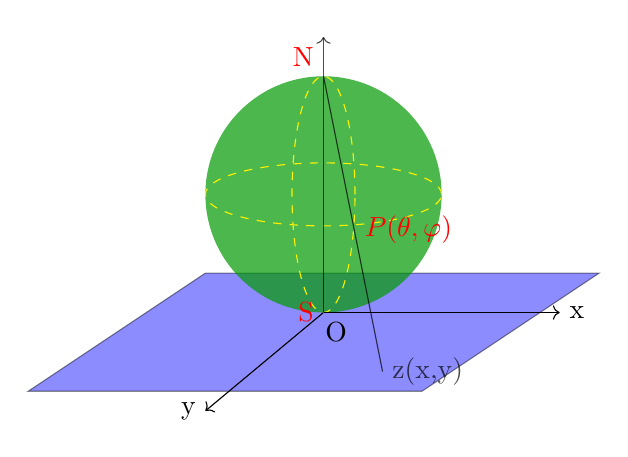
\begin{tikzpicture}[scale=0.5]
    \draw[xslant=1.5, fill=blue, opacity=0.45]
    (0,-5) rectangle (10,-2);
    \node (Center) at (0,0) {};
    \fill[green!60!black, opacity=0.7] (Center) circle (3cm);
    \draw[dashed,draw=yellow ] (Center)  ellipse (3cm and 0.8cm);
    \draw[dashed,draw=yellow ] (Center)  ellipse (0.8cm and 3cm);
    \draw[->, opacity=0.7] (0,-3) -- (0,4) node[right] {};
    \draw[->] (0,-3) -- (-3,-5.5)  node[left] {y};
    \draw[->] (0,-3) -- (6,-3)  node[right] {x};
    \draw[opacity=0.7] (0,3) -- (1.5,-4.5)  node[right] {z(x,y)};
    \node [left,red] at (0,-3)   {S};
    \node [above left,red] at (0,3)   {N};
    \node [right,red] at (0.8,-0.9)   {$P(\theta,\varphi)$};
    \node [right] at (-0.2,-3.5)  {O};
\end{tikzpicture}  
\caption{复球面示意图}
    \label{fig:fqm}
\end{figure}
%\begin{figure}[htbp]
%    \centering
%    \includegraphics[width=0.38\textwidth]{figs/cn6.png}
%    \caption{复球面示意图}
%    \label{fig:fqm}
%\end{figure}
北极$N$与复平面点$z(x,y)$的连线与球面交于点$P(\theta, \varphi)$。很明显,通过这种连线,球面上的点与复平面的点构成一一对应关系。特别地,球面的北极$N$是复平面无穷大$\infty$的几何表示。这样,球面上的每一点都有唯一的一个复数与之对应,因此称为\emph{复球面}。并称点$P(\theta, \varphi)$为复数$z$的\emph{复球面表示}。
\begin{equation}
    z = P(\theta, \varphi)
\end{equation}
包括无穷远点在内的复平面称为\emph{扩充复平面}。不包括无穷远点在内的复平面称为\emph{有限复平面}, 简称复平面。

对于复数$\infty$,它的模规定为正无穷大, 而实部,虚部和辐角等概念均无意义。很明显,复球面表示的优越性在于能把复数$\infty$(或者说复平面无穷远点)显式地表示出来。 对于复数$\infty$,有如下计算规则:
\begin{compactitem}
    \item 加法: $z + \infty = \infty +z = \infty, \quad ( z \ne \infty)$
    \item 减法: $z - \infty = \infty -z = \infty, \quad ( z \ne \infty)$
    \item 乘法: $z \cdot \infty = \infty \cdot z = \infty, \quad ( z \ne 0)$
    \item 除法: $\dfrac{z}{\infty} =0, \, \quad  \dfrac{\infty}{z} =\infty,(z \ne \infty ), \, \quad \dfrac{z}{0} =\infty, (z \ne 0)$
\end{compactitem}

~\\
\begin{hint}
    为适应不同问题的讨论, 复数有六种常见表示:
    \begin{compactitem}
      \item 代数表示 $~ z=x+yi$
      \item 向量表示 $~ z= \overrightarrow{oz}$ 
      \item 三角表示  $~ z=r (\cos \theta + i\sin \theta)$
      \item 指数表示  $~ z= r e^{i \theta}$
      \item 有序实数对表示  $~ z=(x,y)= (r\cos \theta, r\sin \theta )$
      \item 复球面表示 $~ z= P(\theta, \varphi)$
    \end{compactitem}
    它们各有其便, 且可相互转换。具体使用时以直观和方便计算为要。 
\end{hint}
\begin{example}
    试把复数$z=1-i$转化成指数形式。
\end{example}
\emph{解: } 可经三角式过渡
\[ \begin{aligned} 
    z&= \sqrt{2} (\frac{\sqrt{2} }{2} - i\frac{\sqrt{2} }{2}) \\
     &= \sqrt{2} (\cos \frac{1}{4}\pi - i\sin \frac{1}{4}\pi  ) \\
     &= \sqrt{2} [\cos (-\frac{1}{4}\pi) + i\sin (-\frac{1}{4}\pi  )]\\
     &= \sqrt{2}  e^{-i \frac{\pi}{4}} 
\end{aligned}\]
\begin{example}
    试把复数$z=1-\cos \theta + i \sin \theta \quad (0 < \theta \le \pi)$化成指数形式。
\end{example}
\emph{解: }由三角函数公式
\[ \begin{aligned} 
    z&= 1-\cos \theta + i \sin \theta \\
     &= 2 \sin ^2 \frac{\theta}{2}  + 2i \sin \frac{\theta}{2} \cos \frac{\theta}{2}\\
     &= 2 \sin \frac{\theta}{2}  (\sin \frac{\theta}{2}  +  i\cos \frac{\theta}{2} ) \\
     &= 2  \sin \frac{\theta}{2} [ \cos ( \frac{\pi}{2} -\frac{\theta}{2}) + i\sin ( \frac{\pi}{2} -\frac{\theta}{2}) ] \\
     &= 2\sin \frac{\theta}{2} e^{i (\pi-\theta) /2}
\end{aligned}\]

\subsection{复数的运算} ~\\

由于实数是复数的特例, 规定复数的运算法则时应满足一个基本要求,即:复数运算的法则施行于实数时, 应与实数运算的结果相符。同时,复数域是实数域的扩展,复数按新的法则运算时能够满足实数运算的一般定律,比如加法的交换律、结合律,乘法的交换律、结合律和乘法对加法的分配律等。\\

\noindent \emph{复数相等: } 

如果两复数在复平面上对应的点是同一点,则它们相等。
设复数
\[z_1 = (x_1,\, y_1) \qquad z_2=(x_2,\,y_2) \]
则它们相等时,其实部和虚部分别相等
\begin{equation}\label{} 
    {z}_{1}={z}_{2} \quad \Leftrightarrow \quad x_{1}=x_{2}, y_{1}=y_2
\end{equation}
设复数
\[z_1 = r_1 e^{i \theta_1} \qquad z_1 = r_2 e^{i \theta_2} \]
则它们相等时,其模长相等而辐角相差$2\pi$的整数倍
\begin{equation}\label{}
    {z}_{1}= {z}_{2} \quad  \Leftrightarrow \quad  r_1= r_2, \theta_1=2k \pi + \theta_2, \quad k \in \mathbb{Z}   
\end{equation}

\begin{proposition}\label{}
	与实数不同,复数只能判断是否相等,不能比较大小。或者说,只有两个复数同时为实数这种特殊情况下,才能比较大小。
\end{proposition}
\begin{proof}
	设虚数$i$可以和$0$比较大小, 则
\begin{compactitem}
   \item 由复数相等条件,可知 $i \ne 0$
   \item 若 $i>0$, 则 $ -1 = i\cdot i >  0 \cdot i  =0$, 矛盾!
   \item 若 $i<0$, 则 $-i> 0$, 因此 $ -1 = (-i)\cdot (-i) >  0 \cdot 0  =0$, 矛盾!
\end{compactitem}
因此,当两个复数不同时为实数时,不能比较大小。 
\end{proof}

\noindent \emph{复数加法: } 

把复数用向量表示,由向量加法得两复数加法法则,即:两复数的和等于它们的实部和虚部分别相加,如图[\ref{fig:fsjjf}]所示。
  \begin{equation}\label{}
      \begin{aligned}
     z &= z_1 + z_2  \\ 
     &= (x_1, y_1) + (x_2,y_2) \\
     &= (x_1+ x_2,\,  y_1+ y_2) 
    \end{aligned} 
  \end{equation}
  交换律
  \[ z_1 + z_2  = z_2 + z_1 \]
  结合律
  \[ (z_1 + z_2) + z_3  = z_1 +(z_2 + z_3) \]
  \begin{figure}[h]
    \centering
    \begin{minipage}[t]{0.49\textwidth}
        \centering
        \begin{tikzpicture}
            \tikzset{
                %Define standard arrow tip
                >=stealth',
                % Define arrow style
                pil/.style={->,thick}
                }
            \draw[thick,->] (-.5,0) -- (3.5,0) node[anchor=north west] {x};
            \draw[thick,->] (0,-.5) -- (0,3.5) node[anchor=north east] {y};
            \node[anchor=north east] at (0,0) {O};
            \draw[black!60!green,thick,->] (0,0) -- (2,0.5) node[right] {$z_1$};
            \draw[black!60!green,thick,->] (0,0) -- (0.5,2) node[right] at (0.5,1.9) {$z_2$};
            \draw[black!60!green,thick,->] (0,0) -- (2.5,2.5) node[right] {$z_1+z_2$};
            \draw[black!60!green,thick,dashed] (2.5,2.5) -- (2.5,0)  node[below] at (2.8,0) {$x_1+x_2$};
            \draw[black!60!green,thick,dashed] (2.5,2.5) -- (0,2.5)  node[left] {$y_1+y_2$};
            \draw[black!60!green,thick,dashed] (2,0.5) -- (2.0,0)  node[below] {$x_1$};
            \draw[black!60!green,thick,dashed] (2,0.5) -- (0,0.5)  node[left] {$y_1$};
            \draw[black!60!green,thick,dashed] (0.5,2) -- (0,2.0)  node[left] {$y_2$};
            \draw[black!60!green,thick,dashed] (0.5,2) -- (0.5,0)  node[below] {$x_2$};
            \draw[black!60!green,thick] (0.5,2) -- (2.5,2.5);
            \draw[black!60!green,thick] (2,0.5) -- (2.5,2.5);
        \end{tikzpicture}
        \caption{复数加法}
        \label{fig:fsjjf}
    \end{minipage}
    \begin{minipage}[t]{0.49\textwidth}
        \centering
        \begin{tikzpicture}
            \tikzset{
                %Define standard arrow tip
                >=stealth',
                % Define arrow style
                pil/.style={->,thick}
                }
                \draw[thick,->] (-.5,0) -- (3.5,0) node[anchor=north west] {x};
                \draw[thick,->] (0,-2.0) -- (0,2.0) node[anchor=north east] {y};
                \node[anchor=north east] at (0,0) {O};
                \draw[black!60!green,thick,->] (0,0) -- (-0.5,1.5) node[left] {$z_2$};
                \draw[black!60!green,thick,->] (0,0) -- (0.5,-1.5) node[below] {$-z_2$};
                \draw[black!60!green,thick,->] (0,0) -- (2,0.5) node[right] {$z_1$};
                \draw[black!60!green,thick,->] (0,0) -- (2.5,-1) node[right] {$z_1-z_2$};
                \draw[black!60!green,thick] (0.5,-1.5) -- (2.5,-1);
            \draw[black!60!green,thick] (2,0.5) -- (2.5,-1);
        \end{tikzpicture}
        \caption{复数减法}
        \label{fig:fsjjf2}
    \end{minipage}
 \end{figure}
%\begin{figure}[htbp]
%    \centering
%   \includegraphics[width=0.85\textwidth]{figs/cn1.png}
%    \caption{(a)复数的加法,(b)复数减法}
%    \label{fig:fsjjf}
%\end{figure}
\begin{corollary}\label{}
    \noindent 当有$n$个复数相加时
    \begin{equation}\label{} z_1 + z_2  + \cdots + z_n = (\sum_{j=1}^n x_j,\, \sum_{j=1}^n y_i)   
    \end{equation}
\end{corollary}

~\\
\noindent \emph{复数减法: }

减法是加法的逆。取$z_2$ 关于原点的对称点,即得$-z_2$,如图[\ref{fig:fsjjf2}]所示。得复数复数减法法则:
\begin{equation}\label{}
    z_1 - z_2 = z_1 +(-z_2) = (x_1 - x_2, y_1 - y_2) 
\end{equation}
即:两复数的差等于它们的实部和虚部分别做差。
两复数做差,在复平面上对应两个向量$\overrightarrow{z_1 z_2} = z_2 -z_1$ 和 $\overrightarrow{z_2 z_1} = z_1 -z_2$。它们的模相等,方向相反。 

~\\
利用测距算符
\begin{equation}\label{}
    \begin{aligned}
        \hat{d}[z_1, z_2] &= \left\vert z_1 - z_2\right\vert \\
            &=  \left\vert (x_1-x_2, \, y_1-y_2)\right\vert \\
            &= \sqrt{(x_1-x_2)^2 + (y_1-y_2)^2}  
        \end{aligned} 
\end{equation}
因此复数差的模具有复平面两点距离的几何意义, 
若取$z_2 =0$, $z =z_1$, 则有
        \[\left\vert z\right\vert = \hat{d}[z, 0] =  \left\vert \overrightarrow{oz}\right\vert\]
正如前所述,复数$z$的模就是向量$\overrightarrow{oz}$的长度。

~\\
由复数的和差公式,可得三角不等式:
\begin{equation}\label{}
    \begin{aligned}
        (1) &\quad   \left\vert z_1 + z_2 \right\vert \le \left\vert z_1 \right\vert +
        \left\vert z_2 \right\vert \\
        (2) &\quad  |z_1-z_2| \ge |z_1|  - |z_2|  \\
     (3) & \quad  |z_1-z_2| \le |z_1- z|  + |z-z_2|  \\ 
     (4) & \quad \left\vert \left\vert z_1\right\vert - \left\vert z_2\right\vert \right\vert  \le \left\vert z_1 \pm z_2 \right\vert 
     \le \left\vert z_1\right\vert + \left\vert z_2 \right\vert 
\end{aligned} 
\end{equation}
\begin{example}
    试证明不等式
    \[|z_1 -z_2| \ge ||z_1| - |z_2||\]
    \end{example}
\begin{proof}
    设原点$O$与点$z_1$、$z_2$不共线,则它们构成$\Delta Oz_1z_2$。此三角形的边长分别为
    $$a_1 =|z_1 -z_2|, \quad a_2 =|z_1|, \quad a_3 =|z_3|$$
    由于三角形两边长之差小于第三边边长, 因此有 
    \[|z_1 -z_2| > ||z_1| - |z_2||\]
    当三点共线时,有 
    \[|z_1 -z_2| = ||z_1| - |z_2||\]
    原不等式得证。
\end{proof}
\begin{corollary}\label{}
    \noindent 对于n个复数的和,存在不等式
    \begin{equation}
        |z_1 + z_2 + \cdots + z_n| \le |z_1| + |z_2| + \cdots +   |z_n| 
    \end{equation}
\end{corollary}
\begin{example}
    已知$x$是实数,求 
    \[f(x) = \sqrt{(x+4)^2 +4} - \sqrt{x^2 +1}\]
    的极大值
\end{example}
    \emph{解:} 令$z_1 = x+4 + 2i, \quad z_2 = x+i$,则有 
    \[ \begin{aligned}
        f(x) = |z_1| - |z_2| 
          \le |z_1-z_2| 
          = |x+4 + 2i - x -i| 
          = \sqrt{17}
    \end{aligned} \]
    取极值的条件为
    \[ \frac{2}{x+4} = \frac{1}{x}\]
    即$x=4$
\begin{example}
    求复数方程 
    \[\left\vert z+i\right\vert =2\]
    所表示的曲线 
    \end{example}
    \emph{解:} 做简单变换
    \[ \begin{aligned}
       \left\vert z+i\right\vert &=2  \\ 
       \left\vert z- (0-i)\right\vert &=2  \\ 
    \end{aligned} \]
    由测距算符可知,上式描述到定点$(0, -1)$的距离恒为 2 的点的集合,即此复数方程表示复平面上以点$(0, -1)$为圆心半径为2的圆线, 如图[\ref{fig:fbmyx}]所示。
    \begin{figure}[h]
		\centering
        \begin{minipage}[t]{0.49\textwidth}
            \centering
            \begin{tikzpicture}[scale=0.8]
                \tikzset{
                    %Define standard arrow tip
                    >=stealth',
                    % Define arrow style
                    pil/.style={->,thick}
                    }
                \draw[thick,->] (-2.5,0) -- (2.5,0) node[anchor=north west] {x};
                \draw[thick,->] (0,-3.5) -- (0,1.5) node[anchor=north east] {y};
                \node[anchor=north east] at (0,0) {O};
                \draw[black!60!green,thick,name path=l1]  (0,-1) circle (2); 
                \node[right] at(1.2,1.2) {$\left\vert z+i\right\vert =2$};
                \fill[]  (0,-1) circle (2pt); 
                \draw[white,thick,name path=l2]  (0,-1) -- (2,1); 
                \fill[name intersections = {of=l1 and l2,
            name=p}] (p-1) circle (1pt) node [above right] {};
             \draw[black!60!green,thick]  (0,-1) -- (p-1); 
            \end{tikzpicture}
            \caption{复平面圆线}
            \label{fig:fbmyx}
        \end{minipage}
        \begin{minipage}[t]{0.49\textwidth}
            \centering
            \begin{tikzpicture}[scale=1]
                \tikzset{
                    %Define standard arrow tip
                    >=stealth',
                    % Define arrow style
                    pil/.style={->,thick}
                    }
                \draw[thick,->] (-.5,0) -- (3.5,0) node[anchor=north west] {x};
                \draw[thick,->] (0,-.5) -- (0,3.5) node[anchor=north east]  {y};
                \node[anchor=north east] at (0,0) {O};
                \draw[black!60!green,thick,name path=l3] (-0.5,2.5) node[anchor=north] {$z_1$} -- (2.5,0.5) node[anchor=north] {$z_2$};
                \fill[black!60!green]  (-0.5,2.5)  circle (2pt); 
                \fill[black!60!green]  (2.5,0.5) circle (2pt); 
                \draw[white,thick,name path=l4] (0,0) -- (2,2) ;
                \fill[name intersections = {of=l3 and l4, name=p}] (p-1) circle (1pt) node [above right] {};
                \draw[black!60!green,thick]  (0,0) -- (p-1) node [above right] {z}; 
            \end{tikzpicture}
            \caption{复平面线段}
		    \label{fig:fpmxd}
        \end{minipage}
	 \end{figure}

    \begin{example}
        设$z_1, z_2$是复平面两点,试给出下列方程所描述的曲线
        \[ z= z_1 + t (z_2 - z_1), \qquad (0\le t\le 1)\]
    \end{example}
    \emph{解:} 变形,得 
    \[ z -z_1 = t (z_2 - z_1)\]
    向量 $\overrightarrow{z_1 z}$ 与向量 $\overrightarrow{z_1 z_2}$ 共点同向,即$z$点落在由线段$z_1z_2$确定的直线上。参量$t$的取值范围为$(0\le t\le 1)$,因此$z$描述线段$z_1z_2$上的任意点,即方程描述线段$z_1z_2$, 如图[\ref{fig:fpmxd}]所示。

    若改变参量$t$的取值范围: 
    \begin{equation}
        z= z_1 + t (z_2 - z_1), \qquad (-\infty < t < +\infty)
    \end{equation}
则方程描述由$z_1$和$z_2$点确定的直线,并称为复平面上两点确定直线的参数方程。\\
    
\noindent \emph{复数乘法: } 

根据虚数单位运算的约定,得虚数单位$i$的乘法法则:
\[\begin{aligned}
     {i}^1 &= i = (0,1) = e^{i \frac{\pi}{2}}\\
    {i}^2 &= -1 = (-1,0)= e^{i \pi} \\
     {i}^3 &= -i = (0,-1) = e^{i \frac{3\pi}{2}} \\
    {i}^4 &= 1 = (1,0) = e^{i 2\pi }\\ 
\end{aligned} \]
实现的是轴线上四点之间的跳转。因此,$i$的乘法存在周期性
\begin{equation}\label{}
    \begin{aligned}
     i^{4 k}=1,\quad 
     i^{4 k+1}=i,\quad 
     i^{4 k+2}=-1 ,\quad 
     i^{4 k+3}=-i  \qquad (k \in \mathbb{Z}^+)
\end{aligned} 
\end{equation}
数乘
\begin{equation}\label{}
    \begin{aligned}
    i z &= (-y, x) \\
    c z &= (cx, cy)  \\
    ic z &= (-cy, cx) \qquad c \in \mathbb{R}
\end{aligned} 
\end{equation}
复数乘
\begin{equation}\label{}
    \begin{aligned}
    z &= z_1 z_2  \\ 
    &= (x_1, y_1) (x_2,y_2) \\
    &= (x_1x_2- y_1y_2,\,  x_1y_2+x_2y_1) 
   \end{aligned}  
\end{equation}
   交换律
   \[ z_1 z_2  = z_2 z_1 \]
   结合律
   \[ (z_1 z_2)z_3  = z_1 (z_2 z_3) \]
   分配律
   \[ z_1 (z_2 + z_3)  = z_1 z_2 + z_1 z_3\]
采用极坐标表示复数乘法
	\[z= z_1 z_2 = r_{1} e^{\boldsymbol{i}\theta_{1}} \times r_{2} e^{\boldsymbol{i}\theta_{2}} = r_{1} r_{2} e^{\boldsymbol{i}\theta_{1}} e^{\boldsymbol{i}\theta_{2}}\]
    计算后两项的积
    \[ \begin{aligned}
		e^{\boldsymbol{i}\theta_{1}} e^{\boldsymbol{i}\theta_{2}} &=
\left(\operatorname{cos}\left[\theta_{1}\right]+i \operatorname{sin}\left[\theta_{1}\right]\right)\left(\operatorname{cos}\left[\theta_{2}\right]+i \operatorname{sin}\left[\theta_{2}\right]\right) \\
		& =\left(\operatorname{cos}\left[\theta_{1}\right] \operatorname{cos}\left[\theta_{2}\right]-\operatorname{sin}\left[\theta_{1}\right] \operatorname{sin}\left[\theta_{2}\right]+i\left(\operatorname{sin}\left[\theta_{1}\right] \operatorname{cos}\left[\theta_{2}\right]+\operatorname{cos}\left[\theta_{1}\right] \operatorname{sin}\left[\theta_{2}\right]\right)\right) \\
		& =\left(\operatorname{cos}\left[\theta_{1}+\theta_{2}\right]+i \operatorname{sin}\left[\theta_{1}+\theta_{2}\right]\right) \\
		& = e^{\boldsymbol{i}\left(\theta_{1}+\theta_{2}\right)}
		\end{aligned} \]
   得乘法公式 
   \begin{equation}\label{}
       z_1 z_2 = r_{1} r_{2} e^{\boldsymbol{i}\left(\theta_{1}+\theta_{2}\right)} 
   \end{equation}
   分析:
   \[ \begin{aligned}
       \begin{aligned}
           z &= z_2z_1  \\
           &= r_{2} e^{\boldsymbol{i}\theta_{2}} z_1  \\ 
           &= r_{2} [\hat{R}(\theta_{2})z_1] \\
       \end{aligned} 
   \end{aligned}\]
   复数乘法的几何意义:先把$z_1$逆时钟旋转$\theta_2$角,然后把其模伸缩$r_2$倍,如图[\ref{fig:fstimes}]所示。
   \begin{figure}[h]
    \centering
            \begin{tikzpicture}[scale=1]
                \tikzset{
                    %Define standard arrow tip
                    >=stealth',
                    % Define arrow style
                    pil/.style={->,thick}
                    }
                \draw[thick,->] (-.5,0) -- (3.5,0) node[anchor=north west] {$x$};
                \draw[thick,->] (0,-.5) -- (0,3.5) node[anchor=north east]  {$y$};
                \node[anchor=north east] at (0,0) {O};
                % angle \theta_1
                \draw[fill=blue!10] (0,0) -- (0:0.95cm) arc (0:27:.95cm);
                \draw[black!60!green,thick]  (1.15cm,0.15cm) node {$\theta_1$};
                % angle \theta_2
                \draw[fill=blue!20] (0,0) -- (0:0.60cm) arc (0:44:.60cm);
                \draw[black!60!green,thick]  (0.72cm,0.3cm) node {$\theta_2$};
                 % angle \theta
                 \draw[fill=blue!50] (0,0) -- (0:0.35cm) arc (0:73:.35cm);
                 \draw[black!60!green,thick]  (0.3cm,0.47cm) node {$\theta$};
                \draw[black!60!green,thick, ->,name path=l5] (0,0) -- (2,1)  node[right]{$z_1$};
                \draw[black!60!green,thick, ->,name path=l5] (0,0) -- (1.5,1.5)  node[right]{$z_2$}; 
                \draw[black!60!green,thick, ->,name path=l5] (0,0) -- (1.1,3.0) node[right] {$z = z_1 z_2$}; 
            \end{tikzpicture}
    \caption{复数乘法}
    \label{fig:fstimes}
\end{figure}

\begin{corollary}\label{} n个复数的乘法
    \begin{equation}\label{}
        z_1z_2\cdots z_n = (\prod\limits_{j=1}^{n}r_j) \boldsymbol{e}^{\boldsymbol{i} \sum _{j=1}^{n} \theta _j } 
    \end{equation}
\end{corollary}

\begin{corollary}\label{} 复数的乘幂
    \begin{equation}\label{eq:fscft2}
        \begin{aligned}
      z^n &=  r^n e^{i n \theta}\\ 
      &=  r^n (\cos n \theta + i \sin n \theta) , \qquad n \in \mathbb{Z}^+ 
      \end{aligned} 
    \end{equation}
\end{corollary}
\begin{hint}
很明显,复数的乘法既不是向量的点积, 也不是向量的叉积。
\end{hint}

\begin{example}
    设物体受四个力的作用,如图[\ref{fig:fsmsjf}]所示, \\
\begin{figure}[h]
    \centering
    \begin{tikzpicture}[scale=0.6]
        \tikzset{
            %Define standard arrow tip
            >=stealth',
            % Define arrow style
            pil/.style={->,thick}
            }
        \draw[thick,->] (-3.5,0) -- (3.5,0) node[anchor=north west] {$x$};
        \draw[thick,->] (0,-.5) -- (0,4.5) node[anchor=north east]  {$y$};
        \node[anchor=north east] at (0,0) {O};
        \draw[black!60!green,thick,->] (0,0) -- (2.5, 1) node[right]  {$F_1(2.5,1)$};
        \draw[black!60!green,thick,->] (0,0) -- (1, 3) node[right]  {$F_2(1,3)$};
        \draw[black!60!green,thick,->] (0,0) -- (-1, 4) node[left]  {$F_3(-1,4)$};
        \draw[black!60!green,thick,->] (0,0) -- (-3, 1.5) node[left]  {$F_3(-3,1.5)$};
    \end{tikzpicture}
        \caption{复数描述的力}
        \label{fig:fsmsjf}
\end{figure}
%\begin{figure}[h]
%       \centering
%       \includegraphics[width=0.35\textwidth]{figs/c-9.png}
%       \caption{复数描述的力}
%      \label{fig:fsmsjf}
%\end{figure}
试求:
\begin{inparaenum}[(1)]
    \item 合外力的大小和方向,
    \item 若$F_2$逆时针旋转45度, 合外力的大小和方向。
\end{inparaenum}

\end{example}
\emph{解:} (1) 把力写成复数形式, 计算合力 
\[ \begin{aligned}
   F &= (2.5 +1-1-3, 1+3+4+1.5) \\ 
   &= (-0.5, 9.5)
\end{aligned} \]
大小: $\left\vert F\right\vert = \sqrt{0.5^2 + 9.5^2} =9.51 $ \\
方向:$\theta = \arg F + \pi = \pi - \text{argtan} \dfrac{9.5}{0.5}  = \pi - \text{argtan} (19)$ \\
(2) $F_2$逆时针旋转45度
\[ \begin{aligned}
  F'_2 &= \hat{R}(\frac{\pi}{4})(1,3) \\
  &= (1, 1) \cdot (1,3) \\ 
  &= (-2, 4)
\end{aligned}\]
计算合力 
\[ \begin{aligned}
   F &= (2.5 -2-1-3, 1+4+4+1.5) \\ 
   &= (-3.5, 10.5)
\end{aligned} \]
大小: $\left\vert F\right\vert = \sqrt{3.5^2 + 10.5^2} =11.07 $ \\
方向:$\theta = \arg F + \pi = \pi - \text{argtan} \dfrac{10.5}{3.5}  = \pi - \text{argtan} (3)$ \\

\noindent \emph{共轭运算: } 

\begin{example}
    在复平面找点$z$关于$x$轴的对称点$z^*$。
    \begin{figure}[h]
        \centering
        \begin{tikzpicture}[scale=1]
        \tikzset{
        %Define standard arrow tip
         >=stealth',
        % Define arrow style
        pil/.style={->,thick}
        }
                    \draw[thick,->] (-.5,0) -- (4.5,0) node[anchor=north west] {};
                    \draw[thick,->] (0,-2.0) -- (0,2.0) node[anchor=north east] {};
                    \node[anchor=north east] at (0,0) {O};
                    % angle \theta
                    \draw[fill=blue!20] (0,0) -- (0:0.60cm) arc (0:44:.60cm);
                    \draw[black!60!green,thick]  (0.72cm,0.3cm) node {$\theta$};
                    % angle -\theta
                    \draw[fill=blue!20] (0,0) -- (0:0.60cm) arc (0:-44:.60cm);
                    \draw[black!60!green,thick]  (0.72cm,-0.3cm) node {$-\theta$};
                    \draw[black!60!green,thick,->] (0,0) -- (1.5,1.5)  node[right]{$z$}; 
                    \draw[black!60!green,thick,->] (0,0) -- (1.5,-1.5)  node[right]{$z^*$}; 
                    \draw[black!60!green,thick,dashed] (1.5,1.5) -- (0,1.5)  node[left]{$y$}; 
                    \draw[black!60!green,thick,dashed] (1.5,-1.5) -- (0,-1.5)  node[left]{$-y$}; 
                    \draw[black!60!green,thick,dashed] (1.5,1.5) -- (1.5,0) node[right] at (1.5,-0.2) {$x$}; 
                    \draw[black!60!green,thick,dashed] (1.5,-1.5) -- (1.5,0) ; 
                    \draw[black!60!green,thick,->] (0,0) -- (3,0)  node[above] at (3.3,0) {$z+z^*$};
                    \draw[black!60!green,thick] (1.5,-1.5) -- (3,0) ;
                    \draw[black!60!green,thick] (1.5,1.5) -- (3,0) ;
                    \draw[black!60!green,thick,->] (0,0) -- (4,0)  node[below] {$zz^*$};
                \end{tikzpicture}
        %\includegraphics[width=0.2\textwidth]{figs/c-3.png}
        \caption{共轭复数}
        \label{fig:gefs}
    \end{figure} 
\end{example}
很明显
  \begin{equation}\label{}
       z=(x, \, y ),  \qquad z^* = (x, \, -y)   
  \end{equation}
指数形式
  \begin{equation}\label{}
    z= r e^{i \theta}, \qquad  z^*= r e^{-i \theta}
\end{equation}  
我们把实部相同而虚部互为相反数的两个复数称为\emph{共轭复数 },比如: $z^*$与$z$互为共轭复数。
通常也称$z^*$为$z$的共轭复数,记为:$\overline{z} = z^*$, 如图[\ref{fig:gefs}]所示。共轭复数具有如下运算性质:
\begin{equation}\label{}
    \begin{aligned}
    &(1) \, \overline{z_{1} \pm z_{2}}=\bar{z}_{1} \pm \bar{z}_{2} \qquad  (z_{1} \pm z_{2})^* = z_{1}^* \pm z_{2}^* \\
    &(2) \, \overline{z_{1} \cdot z_{2}}=\bar{z}_{1} \cdot \bar{z}_{2}  \hspace{1em} \qquad (z_{1} \cdot z_{2})^* = z_{1}^* \cdot z_{2}^* \\
    &(3) \, \overline{\left(\frac{z_{1}}{z_{2}}\right)}=\frac{\bar{z}_{1}}{\bar{z}_{2}}  \hspace{2em} \qquad \left(\frac{z_{1}}{z_{2}}\right)^* = \frac{z_{1}^*}{z_{2}^*}\\
    &(4) \,\bar{\bar{z}}=z \hspace{5em} \qquad  (z^*)^* = z \\
    &(5) \,z \cdot \bar{z}=\left\vert z\right\vert^2 \hspace{3em} \qquad  z \cdot z^* = \left\vert z\right\vert^2 \\
    &(6) \,z+\bar{z}=2 \operatorname{Re}(z)  \hspace{1em} \qquad  z+z^*=2 \operatorname{Re}(z)  \\
    &(7) \,z-\bar{z}=2 i \operatorname{Im}(z)  \hspace{0.5em} \qquad z-z^*=2 i \operatorname{Im}(z) \\ 
\end{aligned} 
\end{equation}

注意到$z+z^*$和$zz^*$总是实数,而$z-z^*$通常是纯虚数。灵活运用这些公式,可提高复数计算的效率。
\begin{example}
    设$z_1 $ ,$ z_2 $ 是两个任意复数, 试证明 
	\[ \left\vert z_1 + z_2\right\vert ^2 =  \left\vert z_1\right\vert^2 + \left\vert z_2\right\vert^2  + 2 Re(z_1z_2^*)\] 
\end{example}
\begin{proof}
    由模方公式 
	\[ \begin{aligned}
		\left\vert z_1 + z_2\right\vert ^2  &= (z_1 + z_2)(z_1 + z_2)^* \\ 
		&= (z_1 + z_2)(z_1^* + z_2^* ) \\
		&= z_1 z_1^* + z_2 z_2^*  + z_1 z_2^* + z_1^* z_2  \\
		&= z_1 z_1^* + z_2 z_2^* + z_1 z_2^* + (z_1 z_2^*)^*  \\
		&= \left\vert z_1 \right\vert^2 + \left\vert z_2 \right\vert^2 + 2 Re(z_1z_2^*)
	\end{aligned}\]
\end{proof}

\noindent \emph{复数除法: } 

除法是乘法的逆, 对于$z= 1 \cdot z = r e^{i\theta}$,它是由实数单位"1"逆时针旋转$\theta$角后其模再伸缩r倍而来,则$\dfrac{1}{z}$应能把$z$逆变成实数单位"1",即 
\[ \frac{z}{z} = z \cdot \frac{1}{z}  = r e^{i\theta} \cdot \frac{1}{z}   =1 \]
可得
\begin{equation}\label{}
    \frac{1}{z} = \frac{1}{r} e^{i(- \theta)}  = \frac{1}{r} [\cos(-\theta) + i \sin(- \theta)]
\end{equation}
当$z_2 \ne 0$时,有 
\begin{equation}\label{}
    \begin{aligned}
    \frac{z_1}{z_2} &=  \frac{z_1 z^*_2 }{|z_2|^2 }  \\ 
    &= \frac{(x_1, y_1)(x_2, -y_2) }{x^2_2+ y^2_2}   \\
    &= \frac{(x_1x_2 + y_1y_2, x_2y_1 -x_1y_2)}{x^2_2+ y^2_2}   
\end{aligned} 
\end{equation}
极坐标形式
\begin{equation}\label{}
      z = \frac{z_1}{z_2} = \frac{r_1}{r_2} e^{i(\theta _1 - \theta _2)}  
\end{equation}
除法的几何意义:先把$z_1$顺时钟旋转$\theta_2$角,然后再把模伸缩$\dfrac{1}{r_2}$倍。\\
\begin{example}
    已知
	\[ z_1 = \frac{1}{2}(1-i\sqrt{3}), \, z_2 = \sin \frac{\pi}{3} -i \cos \frac{\pi}{3}\]
	求$z_1z_2$ 和 $\dfrac{z_1}{z_2}$
\end{example}
\emph{解: } 把 $z_1, z_2$化成指数形式
\[ \begin{aligned}
    z_1 &= \cos (- \frac{\pi}{3}) + i  \sin  (- \frac{\pi}{3})  = e^{-i \pi /3}\\
    z_2 &= \cos (- \frac{\pi}{6}) + i  \sin  (- \frac{\pi}{6})  = e^{-i \pi /6}\\
\end{aligned}\]
代入乘法公式
\[ z_1 \cdot z_2 = e^{-i (\pi /3 +\pi /6) } = e^{-i \pi /2 } = -i\]
代入除法公式
\[ \dfrac{z_1}{z_2} = e^{i (-\pi /3 + \pi /6) } = e^{-i \pi /6 } \]
\begin{example}
    已知 
	\[ z_1 = \left( \frac{1-i}{1+i}\right)^7 + i, \, z_2 = \frac{i}{1-i} + \frac{1-i}{i}  + \frac{3}{2}\] 
	求 $z_1 \cdot z_2 $ 和$\dfrac{z_1}{z_2}$ 
\end{example}
\emph{解:}(1) 先求出$z_1$ 和$z_2$, 
\[ \begin{aligned}
    \frac{1-i}{1+i} &= \frac{(1-i)(1+i)^*}{|1+i|^2} = \frac{(1-i)^2}{2}  = -i 
\end{aligned}\]
因此
\[ z_1 = (-i)^7 + i = -(i)^3 + i = 2 i\]
由于
\[ \begin{aligned}
    \frac{i}{1-i} + \frac{1-i}{i} &= \frac{i(1+i)}{2} - (1-i)i  = - \frac{3}{2} - \frac{1}{2} i 
\end{aligned}\]
因此 
\[     z_2 = - \frac{3}{2} - \frac{1}{2} i  + \frac{3}{2} = - \frac{1}{2} i\]
(2) $z_1 \cdot z_2 $
\[ z_1 \cdot z_2 = - 2 i \cdot  \frac{1}{2} i =  1 \]
(3) $\dfrac{z_1}{z_2}$
\[ \frac{z_1}{z_2} = - \frac{2 i}{\frac{1}{2} i} = -4 \]
\begin{example}
    试证明平面三角形的内角和等于$\pi$
\end{example}
\begin{proof}
设三角形的三个顶点$z_1, z_2, z_3$对应的内角分别为$\alpha, \beta, \gamma$。则有
\[\alpha = \arg \frac{z_3-z_1}{z_2- z_1}, \, \beta = \arg \frac{z_3-z_2}{z_1- z_2}, \, \gamma = \arg \frac{z_1-z_3}{z_2- z_3}\] 
由于 
\[ \frac{z_3-z_1}{z_2- z_1} \cdot \frac{z_3-z_2}{z_1- z_2} \cdot \frac{z_1-z_3}{z_2- z_3} = -1\]
得
\[\arg \frac{z_3-z_1}{z_2- z_1} + \arg \frac{z_3-z_2}{z_1- z_2} + \arg \frac{z_1-z_3}{z_2- z_3} = \arg(-1) + 2 k \pi = \pi + 2 k \pi\] 
即  \[ \alpha + \beta + \gamma =  \pi + 2 k \pi, \quad \text{k为某适当整数}\] 
又由于$ 0< \alpha,  \beta, \gamma < \pi $,得
\[ 0< \alpha + \beta + \gamma < 3 \pi \]  
两式都成立,必有$k = 0 $, 故而 $\alpha + \beta + \gamma = \pi$
\end{proof}

\noindent \emph{复数的乘幂与方根: }

\noindent (1) 正整数幂 \\
作为乘积的特例, 我们考虑非零复数$z$的正整数次幂,由复数乘法推论[\ref{eq:fscft2}],可得复数乘幂公式的三角表示
\begin{equation}\label{}
    z^n =  r^n (\cos n \theta + i \sin n \theta) , \qquad n \in \mathbb{Z}^+  
\end{equation}
极坐标形式
\begin{equation}\label{}
    z^n =  r^n e^{i n \theta}
\end{equation}
存在性质
\begin{equation}\label{}
\begin{cases}
   \left\vert z^n\right\vert = \left\vert z\right\vert^n \\ 
   \text{Arg } z^n  = n \text{Arg }z
\end{cases}
\end{equation}
当$z$的模$r=1$时, 得\emph{棣莫佛公式 }
\begin{equation}\label{}
     (\cos \theta + i \sin  \theta)^n = \cos n \theta + i \sin n \theta
\end{equation}
~\\
\noindent (2) n-次方根 \\
	设 $z=|r| e^{i \theta }$是非零复数,它的n-次方根为$w = |w| e^{i \phi } $, 即
	\[ \begin{aligned}
		w^n &= z \\ 
		|w| ^n  e^{i n\phi } &= |z| e^{i \theta } 
	\end{aligned}\]
	计算模 
	\[ \begin{aligned}
		|w|^n  &= |z| \\ 
		|w| &= |z|^{\frac{1}{n}}
	\end{aligned}\]
	计算辐角
	\[ \begin{aligned}
		n\phi  &= 2 k \pi +\theta \\ 
		\phi  &= \frac{2 k \pi +\theta}{n} \quad (k=0,1,2,\cdots , n-1)
	\end{aligned}\]
    可得n个解
    \[ \begin{aligned}
     w_0 &= |z|^{\frac{1}{n}} e^{i \frac{\theta}{n}} \\ 
     w_1 &= |z|^{\frac{1}{n}} e^{i \frac{\theta}{n}} e^{i \frac{2\times 1\pi}{n}} = e^{i \frac{2\times1\pi}{n}} w_0  \\ 
     w_2 &= |z|^{\frac{1}{n}} e^{i \frac{\theta}{n}} e^{i \frac{2\times 2\pi}{n}} = e^{i \frac{2\times 2\pi}{n}} w_0  \\ 
     ~~ ~~ & \cdots\cdots\cdots   \\
     w_{n-1} &= e^{i \frac{2\times (n-1)\pi}{n}} w_0 
    \end{aligned}\]
    写在一起, 得n-次方根公式
    \begin{equation}\label{}
        \begin{aligned}
         w_k &= e^{i k\frac{2  \pi}{n}} w_0 \quad (k=0,1,2,\cdots , n-1) 
        \end{aligned} 
    \end{equation}
    令$\varphi = \dfrac{2  \pi}{n}$,则 
    \begin{equation}\label{}
        \begin{aligned}
         w_k = e^{i k \varphi} w_0 \quad (k=0,1,2,\cdots , n-1) 
           \end{aligned} 
    \end{equation}
    写成旋转算符形式
    \begin{equation}\label{}
        \begin{aligned}
               w_k = \hat{R}(k \varphi) w_0 \quad (k=0,1,2,\cdots , n-1)
           \end{aligned} 
    \end{equation}
    说明把$w_0 = |z|^{\frac{1}{n}} e^{i \frac{\theta}{n}} $逆时钟旋转$k$倍$\varphi= \dfrac{2  \pi}{n}$角,既得$w_k$。因此,$w_0, w_1,w_2,\cdots w_{n-1}$正好把$2 \pi$ 分为$n$等份。 
\begin{figure}[htbp]
    \centering
    \begin{tikzpicture}[scale = 2]
        \tikzset{
            %Define standard arrow tip
            >=stealth',
            }
        \draw[->] (-1.3,0) -- (1.3,0) node[below] {$x$}; %作x轴并标上字母
        \draw[->] (0,-1.3) -- (0,1.3) node[left] {$y$}; %作y轴并标上字母
        %\node[below left] at (0,0) {$O$}; %标上原点字母 
        \foreach \t in {0,60,120,180,240,300}{
            \draw[black!60!green,thick] (0,0) -- ({sin(\t +10)},{cos(\t +10)});}
        \draw[black!60!green,thick] ({sin(0 +10)},{cos(0 +10)}) node[above] {$w_1$}-- ({sin(60 +10)},{cos(60 +10)}) node[right] {$w_0$} -- ({sin(120 +10)},{cos(120 +10)}) node[right] {$w_5$} -- ({sin(180 +10)},{cos(180 +10)}) node[below] {$w_4$}  -- ({sin(240 +10)},{cos(240 +10)}) node[left] {$w_3$} -- ({sin(300 +10)},{cos(300 +10)}) node[left] {$w_2$}  -- ({sin(0 +10)},{cos(0 +10)}) ;
        \draw[thick] (0,0) circle(1);
        \draw[fill=blue!20] (0,0) -- (0:0.30cm) arc (0:20:.30cm);
        \draw[black!60!green,thick] (10:0.6cm) node {$\theta/6$};
       \end{tikzpicture}
    %\includegraphics[width=0.4\textwidth]{figs/c-6.png}
    \caption{复数$z$的6-次方根}
    \label{fig:scfg}
\end{figure}
~\\

例如:若取 $n=6$, 则 $ w_0 =  \left\vert z\right\vert ^{\frac{1}{6}} e^{i\frac{\theta}{6}}$, 并且 $\varphi = \dfrac{2  \pi}{6} = \dfrac{\pi}{3}$。取$k=1,2,\cdots ,5$, 然后把$ w_0 $旋转$ k \varphi $得其他五个解。这六个解是圆点在原点半径为$\left\vert z\right\vert ^{\frac{1}{6}} $的圆内接正六边形的顶点, 如图[\ref{fig:scfg}]所示。
    
若令$\omega = e^{i \frac{2 \pi}{n}}$, 有  $\omega^n =1$。则 $1$的$n$-次方根记为$1, \omega, \omega^2, \cdots, \omega^{n-1}$, 由它们在单位圆上的分布对称性,得公式 
    \begin{equation}
        1 + \omega + \omega^2 + \cdots + \omega^{n-1} =0  , \qquad  (\omega^n =1) 
    \end{equation}
特别地,当$n=3$时,有$\omega = e^{i \frac{2 \pi}{3}}  = - \dfrac{1}{2} + \dfrac{\sqrt{3}}{2} i $, 得 
    \begin{equation}
        1 + \omega + \omega^2 =0, \qquad  (\omega^3 =1) 
    \end{equation}
\begin{example}
    试把 $\cos 3\theta$ 分解成 $\cos \theta$ 的表达式 
\end{example}
\emph{解: }由棣莫弗公式
\[ \begin{aligned}
 z &= \cos 3 \theta + i \sin  3 \theta \\
    &= (\cos \theta + i \sin  \theta)^3 \\ 
    &= \cos ^3 \theta  + 3 i \cos ^2 \theta \sin \theta - 3 \cos \theta \sin ^2 \theta - i \sin ^3 \theta \\ 
    &= (\cos ^3 \theta - 3 \cos \theta \sin ^2 \theta ) + i (3  \cos ^2 \theta \sin \theta - \sin ^3 \theta )
\end{aligned}\]
因此有
\[\begin{aligned}
  \cos 3 \theta &=  \cos ^3 \theta - 3 \cos \theta \sin ^2 \theta  \\ 
  &= 4 \cos ^3 \theta - 3 \cos \theta
\end{aligned}\]
\begin{example}
    求$ \sqrt[3]{-8}$的根 
\end{example}
\emph{解:}把-8 写成复数的指数形式
\[ \begin{aligned}
     -8 &= 8 e^{i \pi}  \\ 
\end{aligned}\]
因此, 三次方根为 \[ w = \sqrt[3]{8} e^{i (2k +1)\pi / 3}, \, (k = 0, 1, 2) \]
代入,有
\[ \left\{ \begin{array} {rl}
    w_0 &= 2 e^{i \pi / 3} \\
    w_1 &= -2 \\
    w_2 &= 2 e^{-i \pi / 3}
\end{array} \right.\]
\begin{example}
解复数方程 
\[ (1+z)^5 = (1-z)^5\]
\end{example}
\emph{解:}把 $z=1$ 代入,方程不成立,说明 $z \ne 1$, 因此有 
\[ \begin{aligned}
    (1+z)^5 /(1-z)^5 &=  1 \\ 
    \left( \frac{1+z}{1-z}\right) ^5 &=1 \\
    w ^5 &= 1
\end{aligned}\]
由n-次方公式,有
\[ w = e^{i\frac{2k\pi}{5}} =  e^{i k\varphi\pi} , \quad (k=0,1,2,3,4)\]
 由于
 \[ \frac{1+z}{1-z}= w_k \]
 可得
 \[ \begin{aligned}   
   z &= \frac{w_k -1 }{w_k + 1} = \frac{e^{i k\varphi\pi} -1 }{e^{i k\varphi\pi} + 1}  \\ 
    &= \frac{\cos k \varphi + i \sin k \varphi -1 }{\cos k \varphi + i \sin k \varphi + 1}  \\ 
    &= \frac{2 \sin k\frac{\varphi}{2}\left(-\sin k\frac{\varphi}{2}+i \cos k\frac{\varphi}{2}\right)}{2 \cos k\frac{\varphi}{2}\left(\cos k\frac{\varphi}{2}+i \sin k\frac{\varphi}{2}\right)} \\
    &= i \tan k\frac{\varphi}{2} 
 \end{aligned}\]
 代入$\varphi = \dfrac{2k\pi}{5}, k=0,1,2,3,4 $, 得
 \[ z_0 = 0, z_1= i \tan \frac{\pi}{5} , z_2= i \tan \frac{2\pi}{5}, z_3 = i \tan \frac{3\pi}{5}, z_4 = i \tan \frac{4\pi}{5}\]
\begin{example}
 试证明:三个复数$z_1, z_2, z_3$ 在复平面构成等边三角形的充要条件为
 \[z^2_1 + z^2_2 + z^2_3  = z_1 z_2 + z_2 z_3 + z_3 z_1\]
\end{example}
\begin{proof}
若$\Delta z_1 z_2 z_3$ 是等边三角形,则向量$\overrightarrow{z_1 z_2}$绕$z_1$ 左旋转 $\pi/3$或右旋转 $\pi/3$必得向量$\overrightarrow{z_1 z_3}$
\[\begin{aligned}
    z_3 - z_1  &= (z_2 - z_1)e^{\pm \frac{\pi}{3} i} \\ 
    \frac{z_3 - z_1  }{z_2 - z_1}&= \cos \frac{\pi}{3} \pm i \sin \frac{\pi}{3} \\
    \frac{z_3 - z_1  }{z_2 - z_1} - \frac{1}{2}&= \pm \frac{\sqrt{3}}{2}  i \\
\end{aligned}\]
两边平方并化简,得 
\[z^2_1 + z^2_2 + z^2_3  = z_1 z_2 + z_2 z_3 + z_3 z_1\]
\end{proof}    


\section{复平面的点集}\label{sec:order}

在复数环节,我们已看到复平面上的线段、直线和圆周等都是复平面上的点的集合。复变函数的定义域和
值域通常是复平面上的点集。因此,我们有必要先了解复平面点集的基本概念及相关知识,然后再进入复变函数环节。

复平面的点集可以是由一个个相互孤立的点构成的集合,也可以是由一条直线、线段或一段曲线上的所有连续点构成的集合,也可以是由聚在某个区域内的所有连续点构成的集合。如果用点集所含点的多少来定义点集的大小,则复平面上任意点集$D$的大小记为$|D|$。多个点集的并集可以构成更大的点集,最大的点集是由复平面上所有的点构成的点集$\mathbb{C}$,并称$\mathbb{C}$为\emph{全集}。复平面上任意点集$D$都是全集$\mathbb{C}$的子集。

\subsection{平面点集的几个概念}

\begin{definition}\label{}\index{}
    设$z_0 \in \mathbb{C},  r  \in \mathbb{R} \mid  r  > 0$, 点集$\{z \mid \left\vert z - z_0 \right\vert <  r , z \in \mathbb{C} \}$ 称为$z_0$的$ r $-\emph{邻域}, 记为$U(z_0,  r )$, 其中$z_0$为邻域的中心,$ r $为邻域的半径。并称点集$\{z \mid 0 < \left\vert z - z_0 \right\vert <  r , z \in \mathbb{C} \}$为$z_0$的$ r $-\emph{去心邻域} 。
    \begin{figure}[htbp]
      \centering
      \includegraphics[width=0.9\textwidth]{figs/c-11.png}
      \caption{不等式与邻域:(a)邻域,(b)闭圆,(c)去心邻域 }
        %\label{fig:}
    \end{figure} 
\end{definition}
说明:
\begin{compactitem}
    \item 设 $M \in \mathbb{R} \mid M > 0$, 点集 $\{z \mid M<\left\vert z\right\vert  , z \in \mathbb{C} \}$ 是无穷远点的邻域,记为$U(\infty, M)$。点集 $\{z \mid M<\left\vert z\right\vert < + \infty , z \in \mathbb{C} \}$ 是无穷远点的去心邻域。
    \item 点集$\{z \mid \left\vert z - z_0 \right\vert <  r , z \in \mathbb{C} \}$ 是以$z_0$为圆心$ r $为半径的开圆, 是$z_0$的邻域。
    \item 点集$\{z \mid \left\vert z - z_0 \right\vert \le  r , z \in \mathbb{C} \}$ 是以$z_0$为圆心$ r $为半径的闭圆,不是$z_0$的邻域。
    \item 邻域概念是复数数列与复变函数极限的基础。
\end{compactitem}

\begin{definition}\label{}\index{}
	设点集$D \subset \mathbb{C}$, $z_0 \in \mathbb{C} $, $  r  \in \mathbb{R} \mid  r  > 0 $。 若 $ \forall |U(z_0,  r )\cap D| = \infty $, 则称$z_0$ 为$D$的\emph{聚点}或\emph{极限点}。点集$D$的所有聚点构成的集合记为$D^c$。若$\exists U(z_0,  r )\cap D = \{z_0 \}$, 则称$z_0$为$D$的\emph{孤立点}。
    \begin{figure}[htbp]
        \centering
        \includegraphics[width=0.9\textwidth]{figs/cn2.png}
        \caption{ (a) $z_0 \in D$,(b) $z_0 \notin D$但与$D$相邻,(c) $z_0 \notin D$也不与$D$相邻}
        \label{fig:jdjcd}
      \end{figure} 
\end{definition}
说明:
\begin{compactitem}
    \item 图[\ref{fig:jdjcd}]中 $r,p$取确定值时, 点集$D$确定。(a) $z_0$是$D$的聚点,(b) $z_0 \notin D$, 是点集$D$的聚点,(c)$z_0 \notin D$,不是$D$的聚点,也不是$D$的孤立点。        
    \item 若重新定义点集$D:\{ z_0, \left\vert z - p \right\vert <  r  \}$, 则(c)图的$z_0$依然不是$D$的聚点,但是却是$D$的孤立点。
    \item 孤立点不是聚点。
    \item 以下六种说法彼此等价:\\
    \begin{inparaenum}[(a)]
        \item $z_0$是点集$D$的聚点。\\
        \item $z_0$是点集$D$的极限点。\\
        \item 当$z_0 \notin D$时,在$z_0$的任意领域含有D的无穷多个点。 \\
        \item 在$z_0$的任意领域含有异于$z_0$的且属于D的一个点。 \\
        \item 在$z_0$的任意领域含有属于D的两个点。 \\
        \item 可以从D中取出以$z_0$为极限的数列$z_1, z_2, \cdots, z_n, \cdots$。
    \end{inparaenum} 
\end{compactitem}

\begin{definition}\label{}\index{}
	设点集$D \subseteq \mathbb{C}$, $z_0 \in D $, $  r  \in \mathbb{R} \mid  r  > 0 $。 若 $ \exists U (z_0,  r ) \subset D $, 则称$z_0$ 为$D$的\emph{内点}。 点集$D$的所有内点构成的集合记为$D^\circ $
    \begin{figure}[htbp]
        \centering
        \includegraphics[width=0.95\textwidth]{figs/cn3.png}
        \caption{ (a) $z_0 \in D$ 是内点,(b) $z_0 \notin D$不是内点,(c) $z_0 \in D$不是内点}
        \label{fig:ndacj}
      \end{figure} 
\end{definition}
说明:
\begin{compactitem}
    \item 图[\ref{fig:ndacj}]中,$r,p$取确定值时, 点集$D$确定。(a) $z_0$是$D$的聚点也是$D$的内点,(b) $z_0$是$D$的聚点,不是点集$D$的内点,(c) $z_0$是$D$的聚点,不是$D$的内点。 
    \item  (a)、(b)图中,所有属于点集$D$的点都是内点。(c)图中圆线上的点不是内点。 
\end{compactitem}

\begin{definition}\label{}\index{}
	设点集$D \subseteq \mathbb{C}$, 若由所有内点构成的集合$ D^\circ = D $ 则称$D$为\emph{开集},若 $ D^c \subset D $ 则称$D$为\emph{闭集}。
\end{definition}
说明:对于 $ z_0 \in \mathbb{C}, r  \in \mathbb{R} \mid  r  > 0 $,
\begin{compactitem}
    \item  点集$ \left\vert z - z_0 \right\vert < r$ 是开集。  
    \item  点集$ 0 < \left\vert z - z_0 \right\vert < r$ 是开集。 
    \item  点集$ 0 < \left\vert z - z_0 \right\vert \le r$ 是半开半闭集。   
    \item  点集$ \left\vert z - z_0 \right\vert \le r$ 是闭集。 
    \item 全集$\mathbb{C}$是开集。 
    \item $\{z  \mid |z| \ne 0 \}$是开集。
    \item $\{z  \mid |z| \ne 1 \}$是开集。
    \item 点集 $\{z  \mid |z - z_0| = 1 \}$是曲线,不是开集。
    \item 若属于点集D的所有点都是内点,则D必是开集。
\end{compactitem} 

\subsection{区域与曲线}~\\

由孤立的点构成的点集就象星星点点的繁星集。而由非孤立的点构成的点集通常有两种结构:一类是多点聚集而成的块状结构,另一类是点-点相连构成的线状结构。
\begin{definition}\label{}\index{}
	设点集$D \subset \mathbb{C}$, 若$D$满足条件: 
    \begin{inparaenum} [(i)]
        \item $D$是一个开集,
        \item $D$是连通的,
    \end{inparaenum}
    则称$D$为一个\emph{区域} 

    \emph{连通: }是指$D$中的任意两点都可以用某曲线$C$相连接,且$C \subset D$。
    \begin{figure}[htbp]
        \centering
        \includegraphics[width=0.4\textwidth]{figs/cn4.png}
        \caption{区域示意图}
        %\label{fig:}
      \end{figure} 
\end{definition}
说明:若 $z, z_0, z_1$ 都是复数,则
\begin{compactitem}
    \item 点集$\{z  \mid |z- z_0| \ne 0 \}$是开集,是连通的, 是一个区域。
    \item 点集$\{z  \mid |z - z_0| \ne 1 \}$是开集,是不连通的,不是一个区域。
    \item 点集$\{z  \mid |z - z_0| = 1 \}$是曲线,不是开集,是连通的,不是一个区域。
    \item 点集$\{z  \mid |z-z_0| < 1 \} \cup \{z  \mid |z-z_1| < 1 \} $ 是开集,\\
    \begin{inparaenum}[(a)]
        \item 在$|z_1 -z_0| < 2$时连通的,是一个区域。
        \item 在$|z_1 -z_0| \ge 2$时不连通的,不是一个区域。 
    \end{inparaenum} 
    \item 区域是确定复变函数定义域及值域的基础。
\end{compactitem}

\begin{definition}\label{}\index{}
	设区域$D \subset \mathbb{C}$, $z_0 \notin D $, $  r  \in \mathbb{R} \mid  r  > 0 $。若 $ \forall  r , |U(z_0,  r )\cap D|> 0 $,则称$z_0$为区域$D$的边界点。区域$D$的所有边界点构成的集合,称为区域$D$的\emph{边界},记为 $\partial  D$。并称区域$D \cup \partial  D$为\emph{闭域}$D$ 
\end{definition}
说明:若 $z, z_0, z_1$ 都是复数,则
\begin{compactitem}
    \item 点集$\{z  \mid |z- z_0| \ne 0 \}$是一个区域, 它的边界只含一个点$z = z_0$。
    \item 点集$\{z  \mid |z - z_0| \ne 1 \}$不是一个区域,边界没有定义。
    \item 点集$\{|z| < 1 \}$ 是一个区域,边界为曲线$|z|=1$。
    \item 点集$\{z  \mid 0.1 <|z - z_0| < 1 \}$是一个区域,边界为$\{z  \mid |z| =0.1\} \cup \{z  \mid |z| =1\} $。
    \item 点集$\{|z| \le 1 \}$是一个闭域。
    \item 孤立点必是边界点,必属于边界。
    \item 区域都是开的,边界点不属于区域。
\end{compactitem}

\begin{example}
    试判定下列不等式所描述的点集是什么图形,是不是区域,若是则给出它的边界。 
    \[ (1) \Im z >0,\, (2) \Re z <0,\, (3) 1 < \Im z < 2,\, (4) 1 < \Im z \le 2\]
\end{example}
\emph{解:} (1)是实轴以上的上半z平面,是区域, 边界为$C = \{ z \mid z = x+yi, y =0\}$。\\
(2)是虚轴以左的左半z平面,是区域, 边界为$C = \{ z \mid z = x+yi, x =0\}$。\\ 
(3)是界于两直线$y=1$和$y=2$之间的带形区间,是区域,边界为$C = \{ z \mid z = x+yi, y =1\} \cup \{ z \mid z = x+yi, y =2\}$。\\
(4) 是界于两直线$y=1$和$y=2$之间的带形区间(含$y=2$),不是区域, 是半开半闭域。

\begin{definition}\label{}\index{}
	如果区域$D$可以被一个以原点为圆心的圆所包围,则称$D$为\emph{有界区域}。
\end{definition}
说明:若 $z \in \mathbb{C}$,则
\begin{compactitem}
    \item  无界区域: 全集$\mathbb{C}$;$\{z \mid z \ne 0 \}$; $\{z \mid  |Re (z)| < 1 \}$
    \item  有界区域: $\{z \mid |z| < 1 \}$; $\{z \mid |z - z_0| < 1, z_0 \in  \mathbb{C} \}$; $\{z \mid  |Re (z)| < 1,  |Im (z)| < 1 \}$
\end{compactitem}  

\begin{figure}[htbp]
    \centering
    \includegraphics[width=0.33\textwidth]{figs/c-13.png}
    \caption{曲线 $ C: z = z(t)$}
    \label{fig:qxadd}
\end{figure}

\begin{definition}\label{}\index{}
	如果$x(t)$和$y(t)$是两个连续的实变函数,则点集
    \[ z(t) = x(t) + i y(t) \qquad (a\le t \le b)\]
    构成复平面上的一条曲线,称为\emph{连续曲线}, 记为$ C: z = z(t)$,并称 $z(a)$和$z(b)$为曲线$C$的两个\emph{端点}。如图[\ref{fig:qxadd}]所示。
\end{definition}

\begin{definition}\label{}
	对于平面曲线$ C = \{z \mid z=  x(t) + i y(t), a\le t \le b \}$, 如果满足:
	\begin{inparaenum}[(i)]
		\item 导函数$x'(t)$ 和 $y'(t)$ 都是连续的,
		\item 对任意 $t$, 存在$[x'(t)]^2 + [y'(t)]^2 \ne 0$.
	\end{inparaenum}
    则称$C$是\emph{光滑曲线}。由有限条依次相接的光滑曲线所组成的曲线称为按段光滑曲线。
\end{definition}

\begin{definition}\label{}
	设平面曲线$ C = \{z \mid z=  z(t), a\le t \le b \}$, 对于满足
    $a< t_1 < b, a\le t_2 \le b $的参量$t_1$和$t_2$而言, 当 $t_1 \ne t_2$时,若存在 $z(t_1) = z(t_2) $, 则称$z(t_1)$为曲线C的一个\emph{重点}。没有重点的曲线称为\emph{简单曲线},也称\emph{若尔当曲线}。对于简单曲线$ C = \{z \mid z=  x(t) + i y(t), a\le t \le b \}$,若$z(a) = z(b) $,则称$C$为\emph{简单闭曲线}。
\end{definition}
\begin{figure}[h]
    \centering
    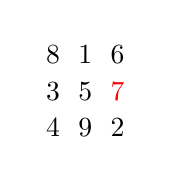
\begin{tikzpicture}
        \matrix[matrix of nodes]
        {
          8 & 1 &         6 \\
          3 & 5 & |[red]| 7 \\
          4 & 9 &         2 \\
        };
      \end{tikzpicture}
    %\includegraphics[width=0.35\textwidth]{figs/c-16.png}
    \caption{若尔当定理} 
    \label{fig:nrddl}
\end{figure}

\begin{theorem}[若尔当定理]\label{} \index{}
	任意一条简单闭曲线$C$把复平面$z$唯一地分成三个互不相交的点集 :
	\begin{inparaenum}[(i)]
	  \item $C$, 所有$C$上的点。
	  \item $I(C)$, 所有$C$内部的点。
	  \item $E(C)$, 所有$C$外部的点。
	\end{inparaenum}
    其中 $I(C)$ 是一个有界区域, $E(C)$ 是一个无界区域。若简单折线$P$的一个端点
	属于$I(C)$ , 另一个端点属于$E(C)$, 则$P$ 必与$C$ 有交点. 如图[\ref{fig:nrddl}]所示。
\end{theorem}
说明:图[\ref{fig:nrddl}]中,
\begin{compactitem}
    \item 点集$C$是曲线,不是区域。
    \item 点集$C$是区域$I(C)$的边界,也是区域$E(C)$的边界。
\end{compactitem}

\begin{definition}\label{}\index{}
	对于区域 $D$,如果由属于$D$的点构成的任意一条简单闭曲线 $C$,都有$I(C)\subset D $,则称$D$为\emph{单连通区域},否则为\emph{多连通区域}。如图[\ref{fig:ntqu}]所示。
    \begin{figure}[h]
        \centering
        \includegraphics[width=0.75\textwidth]{figs/c-17.png}
        \caption{(a) 多连通区域,(b) 单连通区域}
        \label{fig:ntqu}
    \end{figure}
\end{definition}
说明:\begin{compactitem}
    \item 单连通区域是没有所谓的“洞”结构的区域,
    \item 是否存在在拓扑学中非常重要。
\end{compactitem}

\begin{definition}\label{}
	设闭集C是所含不止一个点的点集, 如果不能划分为两个无公共点的非空闭集,则称C为\emph{连续点集}。 若区域D的边界$\partial D$是一个或二个、三个、$\dots$、n个互不相交的连续点集构成,则称D为单连通区域或\emph{二连通、三连通、$\dots$、n连通区域}。
\end{definition}
说明:\begin{compactitem}
    \item 图[\ref{fig:ntqu} (a)]的边界含三个互不相交的连续点集,因此是三连通区域
    \item 洞的数目在拓扑学中也非常重要。
\end{compactitem}

\begin{example}
    指明下列不等式所确定的区域, 是有界的还是无界的,单连通的还是多连通的
    \[ \begin{aligned}
        & (1) Re(z^2) < 1, \qquad (2) |\arg z| < \pi/3, \qquad (3) |1/z| < 3 \\
        & (4) |z+1| +|z-1| <4, \qquad (5) |z-1|\cdot|z+1|<1 , \qquad (6) |z+ 1 +i| <1
    \end{aligned}\]
\end{example}
\emph{解:} (1) 取 $z=x+yi$
\[ \begin{aligned}
    Re(z^2) &= x^2 -y^2 \\
    Re(z^2) < 1 & \quad \Leftrightarrow  \quad  x^2 -y^2 < 1
\end{aligned}\]
这是双曲函数之间的部分, 因此是无界单连通区域。\\
(2) 取 $z=re^{i \theta}$
\[ \begin{aligned}
    |\arg z| < \pi/3 & \quad \Leftrightarrow  \quad  -\pi/3  <\theta < \pi/3 
\end{aligned}\]
这是一个角形域,也是一个无界单连通区域。\\
(3)变形
\[ \begin{aligned}
    |1/z| < 3  & \quad \Leftrightarrow  \quad  |z| > 3 
\end{aligned}\]
这是一个以原点为圆心半径为$\dfrac{1}{3}$的圆的外部区域,是一个无界二连通区域。\\
(4) $|z+1| +|z-1| <4$ \\
这是复平面到两定点的距离和为4的椭圆的内部区域, 因此是有界单连通区域。 \\
\begin{figure}[htbp]
    \centering
    \includegraphics[width=0.4\textwidth]{figs/cn5.png}
    \caption{双叶玫瑰线}
    %\label{fig:}
\end{figure}
(5) $|z-1|\cdot|z+1|<1$\\
取三角式,先计算边界 
\[ \begin{aligned}
    |z-1|\cdot|z+1| &=1 \\
    |r \cos \theta -1 + r i \sin \theta|\cdot|r \cos \theta +1 + r i \sin \theta| &=1 \\
    [(r \cos \theta -1)^2  + (r \sin \theta)^2 ] \cdot [(r \cos \theta +1)^2  + (r \sin \theta)^2 ] &=1 \\
    (r^2 +1)^2 -4(r \cos \theta)^2 &= 1 
\end{aligned}\]
得两个解: (i) $r=0$; (i) $r^2=2 \cos 2 \theta$, 这是双叶玫瑰线。 
\[|z-1|\cdot|z+1| <1 \]
是内部区域,注意到$r=0$连通左右,是有界单连通区域。\\
(6) $ 0<|z+ 1 +i| <1$ \\
是以($-1,-i$)点为圆心半径为$1$的圆的内部去心区域,是有界二连通区域。


\section{复变函数} 
复变函数是以复数为自变量的函数,是十九世纪数学研究的热点。它可以看作是高数中实变函数向复数域的扩充。因此,它的部分内容,如函数可导和解析的判定、函数积分、幂级数的展开等,与高数相应部分内容是极为相似的。但也有部分内容与实变函数明显不同。学习和使用时,要特别注意这些不同的地方。

复变函数重点在于函数的可微性与可积性,这在处理许多物理与工程问题上,有着天然的优势。如关于瑕积分的计算,就有着化繁为简的奇效。

\subsection{复变函数的定义}

\begin{definition}\label{}\index{}
	设$E$为一复数集, 如果存在某种对应关系$f$, 按照这种对应关系,对于$E$中的每一复变数$z= x+yi$, 都存在复变数$w = u+vi $与之对应,则称复变数$w$是复变数$z$的函数,简称\emph{复变函数}, 并记作 $$w = f (z ), \quad (z \in E)$$ 
	若对每个$z$都只存在惟一的复变数$w$与之对应, 则称 $f (z )$是\emph{单值复变函数};若存在两个或两个以上的 $w$与一个$z$对应的情况, 则称 $f (z )$是\emph{多值复变函数}。称$E$为函数$f ( z )$的\emph{定义域}, 并称$w$的所有值构成的集合$F$为函数$f ( z )$的\emph{值域},记为
    \[F: \left\{ w \mid w=f(z), z \in E \right\} \]
\end{definition}
说明:\begin{compactitem}
    \item 只要$E$中有一个$z$存在两个或两个以上的$w$与之对应的情况, $f (z )$就是多值复变函数。
    \item 单值函数要求每一个$z$只有惟一一个$w$与之对应,并没有要求$w$也只有惟一一个$z$与之对应。因此对于单值函数,存在$|F| \ge |E| $。
    \item 复自变量$z$和复因变量$w$之间的关系 $w = f (z )$可用两个二元实变函数
    \[ u =u(x,y), \quad  v =v(x,y)\]
    进行描述。
\end{compactitem}
比如,设$ w = f(z)$取如下具体形式 
\[ w = z^2 +2\]
若$z$采用三角表示,$w$采用代数表示,则有
   \[ \begin{aligned}
	 u+vi &=  r^2 (\cos \theta +i\sin \theta )^2 +2 \\ 
	 &= (r^2 \cos 2 \theta +2) + i r^2 \sin 2 \theta 
   \end{aligned}\] 
根据复数相等条件, 有
   \[ \begin{cases}
	 u = u(r,\theta) = r^2 \cos 2 \theta +2\\
	 v = v(r,\theta) =  r^2 \sin 2 \theta
 \end{cases}\]
 复变函数$w = f (z )$体现的是$(r, \theta)$与($u,v$)之间的对应关系。\\

 若两者都采用有序数对表示,则有
\[ \begin{aligned}
  (u,v)&= (x,y)^2 +(2,0) \\ 
  (u,v)&= (x^2 -y^2 +2,2xy)
\end{aligned}\] 
当然,可以写成
\[ \begin{cases}
  u = x^2 -y^2 +2\\
  v = 2xy
\end{cases}\]
复变函数$w = f (z )$体现的是有序自变量对($x,y$)与有序因变量对($u,v$)之间的关系, 它们构成四维空间 $( u , v , x , y )$ , 因此它们的关系难以在二维空间进行几何表示。如果把有序数对($x,y$)看成$z$-平面的点,有序数对($u,v$)看成$w$-平面的点, 则变成了点与点之间的对应。复变函数$w = f (z )$可看成$z$-平面的点集$E$与$w$-平面的点集$F$之间的关系。如图[\ref{fig:twopoint}]所示。
\begin{figure}[ht]
	\centering
	  \includegraphics[width=0.75\textwidth]{figs/c-18.png}
      \caption{复变函数描述两平面点集间的对应关系}
      \label{fig:twopoint}
\end{figure}
很明显,两点集的元素间有如下关系:
\begin{compactitem}
    \item 对于点集$E$中的每一点$z$, 相应的点$w = f ( z )$必是点集$F$
    中的一个点,
    \item 对于点集$F$中的每一点$w$, 在点集$E$中至少有一点$z$与之对应。
 \end{compactitem}

\begin{definition}\label{}\index{}
	如果用$z$-平面的点$z$表示自变量$z$的值, 而用$w$-平面的点$w$表示因变量$w$的值,那么复变函数$w = f(z)$在几何上可以看作从$z$-平面点集$E$到$w$-平面点集$F$的\emph{变换}。通常称为由函数$w = f(z)$构成的\emph{映射},并称$w$是$z$的\emph{像点},$z$是$w$的\emph{原像}。 
\end{definition}
\begin{figure}[htbp]
	\centering
	\includegraphics[width=0.7\textwidth]{figs/c-19.png}
	\caption{$\Delta ABC $与$\Delta A'B'C' $的映射关系}
	\label{fig:twotri}
  \end{figure}
  图[\ref{fig:twotri}]描述了,$z$平面$\Delta ABC $,通过函数$w = z^* $映射到了$w$平面$\Delta A'B'C' $的情况。原来四维的复杂的对应关系就这样轻松地用二维映射进行了图形化、形象化地描述。

\begin{example}
    把平面$\Delta ABC $绕点$(-2,1)$逆时针旋转45度, 得$\Delta A'B'C' $,如图[\ref{fig:twotri2}]所示。试写出它们之间的变换关系式。
\end{example}
\emph{解:}~$\Delta ABC$ 构成$z$平面点集$E$,$\Delta A'B'C'$ 构成$w$平面点集$F$,令$z_0 = (-2,1)$, 则有
\[ \begin{aligned}
    w-z_0 &= e^{i\pi /4}(z-z_0) \\
    w &=  (z-z_0)e^{i\pi /4} + z_0
\end{aligned} \]  
这正是两者之间的变换关系式。
\begin{figure}[htbp]
    \centering
    \includegraphics[width=0.6\textwidth]{figs/c-20.png}
    \caption{三角形的旋转变换}
    \label{fig:twotri2}
   \end{figure}

若绕点$(-2,1)$逆时针旋转45度并放大10倍,则有
\[ \begin{aligned}
    w-z_0 &= 10 e^{i\pi /4}(z-z_0) \\
    w &=  10 (z-z_0)e^{i\pi /4} + z_0
\end{aligned} \]    

\begin{example}
    在$z$平面有(1)双曲线$x^2 - y^2 =4$ 、(2)直线 $ y= \sqrt{3} x $ (3)圆弧 $\{(x,y) \mid x^2 + y^2 =4, x \ge 0, y \ge 0 \}$, 如图[\ref{fig:threetran}]所示。
	若通过函数$w= z^2 $进行映射,求它们在$w$平面的图像。
    \begin{figure}[htbp]
     \centering
     \includegraphics[width=0.8\textwidth]{figs/c-22.png}
     \caption{(a) z平面曲线, (b) w平面曲线}
     \label{fig:threetran}
    \end{figure}
\end{example}
\emph{解:} (1)由对应关系
\[ \begin{aligned}
    w &=z^2 \\ 
    u+v i &= (x^2 -y^2) + 2 xy i 
\end{aligned}\]
得 $$u = x^2 -y^2 =4$$
因此双曲线$x^2 -y^2 =4$在$w$平面对应直线$u=4$。\\
(2) 直线 $ y= \sqrt{3} x $的辐角为 $\theta _1 = \dfrac{1}{3} \pi, \theta _2 = \dfrac{1}{3} \pi + \pi $,
对应关系 $w =z^2 $要求辐角变成原来的二倍,即
$$\varphi _1  =  2 \theta _1 = \frac{2}{3} \pi \qquad \varphi _2 = 2 \theta _2 = \frac{2}{3} \pi + 2\pi = \varphi _1 $$
因此直线 $ y= \sqrt{3} x $在$w$平面对应一条射线 \\
(3) 圆弧 $\{(x,y) \mid x^2 + y^2 =4, x \ge 0, y \ge 0 \}$ 的复数表示
\[ z= 2 e^{i \theta}, \quad  (0 \le \theta \le \frac{\pi}{2}) \]
由对应关系
\[ \begin{aligned}
    w &=z^2 \\ 
    &= 4 e^{i 2 \theta} \\
    &= R e^{i \varphi}, \quad ( R=4, 0 \le  \varphi \le \pi)
\end{aligned}\]
因此此圆弧在$w$平面对应半圆。\\

\begin{example}
    试问函数$w = \dfrac{1}{z+1}$把z平面的下列曲线变换成了w平面的什么图形?
    \[ (1) x^2 + y^2 =1, \quad (2) y=x+1\]
\end{example}
\emph{解:} (1) 把公式 
\[ x= \frac{1}{2}(z + z^*), \qquad  y= \frac{1}{2i}(z - z^*) \]
代入,$x^2 + y^2 = 1$  有
\[ \frac{1}{4}(z + z^*)^2 - \frac{1}{4}(z - z^*)^2 =1\]
得$zz^* =1$\\
由变换关系 $w = \dfrac{1}{z+1}$, 得
\[ z=  \dfrac{1}{w} -1\]
代入上式
\[ \begin{aligned}
    (\dfrac{1}{w} -1)(\dfrac{1}{w^*} -1) &= 1
\end{aligned} \]
解得$w + w^* =1$, 因此有 
\[ u= \dfrac{1}{2}\]
即:z平面的圆$ x^2 + y^2 =1$被变换成了w平面的直线$u= \dfrac{1}{2}$ \\
(2) 把公式代入$y=x+1$,得
\[ \frac{1}{2i}(z - z^*) = \frac{1}{2}(z + z^*) +1 \]
把 $z=  \dfrac{1}{w} -1$ 代入上式,
\[ \frac{1}{2i} \left( \frac{1}{w} -  \frac{1}{w^*} \right)  =  \frac{1}{2} \left( \frac{1}{w} + \frac{1}{w^*} -2\right) +1 \]
两边同乘$2iw^* w^*$, 得
\[ w^* - w = i(w + w^*)\]
由 $ w -u = iv, \quad  w^*-u = - iv $, 可得
\[ w^* - w = -2 i v, \quad w^* + w = 2 u\]
代回,得 
\[ u = -v \]
即:z平面的直线$y=x+1$被变换成了w平面的直线$u= -v $ \\

\begin{example}
    在$z$平面有点集$\{ z \mid z = x+yi, \, x \in \mathbb{Z}, y \in \mathbb{Z}, \left\vert x \right\vert \le 3, \left\vert y \right\vert \le 3) \}$ 
    若通过函数 $w= e^z $ 进行映射,求它们在$w$平面的图像。
    \begin{figure}[htbp]
        \centering
        \includegraphics[width=0.8\textwidth]{figs/c-24.png}
        \caption{(a) z平面点集,(b) w平面点集}
        \label{fig:twoplantdots}
       \end{figure}
\end{example}
\emph{解:} (1)由对应关系 
\[ w= e^z = e^xe^{iy} =Re^{i\theta}\]
得模长
\[ R= e^3, e^2, e^1, e^0, e^{-1}, e^{-2}, e^{-3}\]
辐角
\[ \theta = -3, -2, -1, 0, 1, 2, 3\]
实现的是49点构成的点集从直角坐标系到极坐标系的变换,如图[\ref{fig:twoplantdots}]所示。\\

\begin{definition}\label{}\index{}
	设函数$w = f(z)$ 的定义集为$z$-平面的点集$E$, 函数值集为$w$-平面的点集$F$,那么$F$中的每个点必将与$E$中的一个或多个点对应。 因此在点集$F$也可确定一个函数$z= \varphi(w)$, 它是函数$w = f(z)$的\emph{反函数},也称映射$w = f(z)$的\emph{逆映射}。记为$z= f^{-1}(w)$。 逆映射是从$w$平面点集$F$到$z$平面点位集$E$之间的变换。
\end{definition}
说明:\begin{compactitem}
    \item 必存在 $\forall w \in F, w = f[\varphi(w)]$,
    \item 当反函数是单值函数时, 必存在 $\forall z \in E, z = \varphi [f(w)]$,
    \item 当函数与反函数都是单值时,则集合$E$和$F$之间构成一一映射。
\end{compactitem} 
~\\

\subsection{复变函数的极限}~\\

\begin{definition}\label{}\index{}
    设函数$w = f(z)$定义在$z_0$的去心领域$0<\left\vert z - z_0\right\vert < \rho $内,如果存在确定的数$w_0$, 对于任意给定的$\varepsilon >0 $, 相应地必有一个实数$\delta $,使得只要
    \[ 0<\left\vert z - z_0\right\vert < \delta, ( 0< \delta \le \rho )  \]
    都有 $\left\vert f(z) -w_0\right\vert < \varepsilon , $ 则称 $w_0$为函数 $f(z)$ 当 $z $趋于$z_0$ 时的\emph{极限},记为:
    \[ \lim_{z \to z_0} f(z) = w_0\] 
\end{definition}
说明:\begin{compactitem}
    \item 若极限 $\lim\limits_{z \to z_0} f(z) = w_0$
	存在,则必然唯一,与$z \to z_0$ 的具体路径无关。
    \item 当$z$-平面的变点$z$进入一个充分小的$z_0$的$\delta $-去心邻域时, 它在$w$-平面的像点就落入$w_0$ 的一个任意给定的 $\varepsilon$-邻域内。如图[\ref{fig:qxry}]所示。
    \begin{figure}[htbp]
      \centering
      \includegraphics[width=0.7\textwidth]{figs/c-23.png}
      \caption{趋于方式的任意性示意图}
      \label{fig:qxry}
    \end{figure} 
    \item 极限的存在是研究复变函数一切重要性质的前提。
\end{compactitem}

\begin{theorem}\label{} \index{}
    设$f(z) = u(x,y) + i v(x,y), z_0 = x_0 + i y_0, w_0 = u_0 + i v_0$,那么存在极限$ \lim\limits_{z \to z_0} f(z) = w_0 $ 的充要条件为:两实变函数$u(x, y), v(x,y)$ 在点($x_0, y_0$)处存在极限
    \[ \lim _{\substack{x \rightarrow x_{0} \\ y \rightarrow y_{0}}} u(x, y)=u_{0}, \quad \lim _{\substack{x \rightarrow x_{0} \\ y \rightarrow y_{0}}} v(x, y)=v_{0}\]
\end{theorem}
说明:\begin{compactitem}
    \item 该定理把复变函数的极限问题转化为两个二元实变函数的极限问题。
    \item 二元实变函数的极限具有惟一性,与$x \rightarrow x_{0} $ 及$y \rightarrow y_{0} $ 的具体路径无关。
\end{compactitem}

\begin{proof}
  (1) 必要性:如果存在$ \lim\limits_{z \to z_0} f(z) = w_0 $ ,根据定义,当$z$进入$\delta$-领域时 
  $$0<\left\vert (x+iy) - (x_0+iy_0)\right\vert < \delta$$
  则$w$必进入$\varepsilon$-领域
  $$\left\vert (u+iv) - (u_0+iv_0)\right\vert < \varepsilon$$
  也就是说
  $$\left\vert (u-u_0) + i(v-v_0)\right\vert < \varepsilon$$
  可得 
  $$\left\vert u-u_0\right\vert < \varepsilon,\quad \left\vert v-v_0\right\vert < \varepsilon$$
  根据实变函数极限的定义,即存在 
  \[ \lim _{\substack{x \rightarrow x_{0} \\ y \rightarrow y_{0}}} u(x, y)=u_{0}, \quad \lim _{\substack{x \rightarrow x_{0} \\ y \rightarrow y_{0}}} v(x, y)=v_{0}\]
  (2)充分性:若
  \[ \lim _{\substack{x \rightarrow x_{0} \\ y \rightarrow y_{0}}} u(x, y)=u_{0}, 
  \quad \lim _{\substack{x \rightarrow x_{0} \\ y \rightarrow y_{0}}} v(x, y)=v_{0}\]
  则必有$$ \left\vert u - u_0 \right\vert  < \dfrac{\varepsilon}{2},\qquad  \left\vert v - v_0 \right\vert  < \dfrac{\varepsilon}{2} $$
  因此 
  $$ \left\vert u - u_0 \right\vert  + \left\vert v - v_0 \right\vert  <  \varepsilon $$
  那么,根据三角不等式,有 
  \[ \left\vert w -  w_0   \right\vert  \le \left\vert u - u_0 \right\vert  +  \left\vert v - v_0 \right\vert < \varepsilon\]
  说明当 $0<\left\vert z- z_0 \right\vert < \delta$时,$w$进行了任意小的$\varepsilon$-领域, 也即
  \[ \lim\limits_{z \to z_0} f(z) = w_0 \]
\end{proof}

\begin{theorem}\label{} \index{}
    若定义于点集$E$的两函数 $f(z), g(z)$ 在 $z_0$ 存在极限
	  \[\lim_{z \to z_0} f(z) = w_{1}, \, \lim_{z \to z_0} g(z) = w_{2}, \]
	  则它们的各、差、积、商也存在极限
	  \[ \begin{aligned}
		 \lim\limits_{z \to z_0} [f(z) \pm g(z)] &= w_{1} \pm w_{2} \\
		 \lim\limits_{z \to z_0} [f(z)g(z)] &= w_{1}w_{2} \\
			\lim\limits_{z \to z_0} [f(z)/g(z)] &= w_{1}/w_{2} 
	  \end{aligned}\]
\end{theorem}
说明:\begin{compactitem}
    \item 复变函数极限四则运算法则与实变函数的类似。
\end{compactitem}
\begin{example}
    试证明, 当$z\to 0$时,函数 $f(z) = \dfrac{Re(z)}{\left\vert z\right\vert}$的极限不存在
\end{example}
\begin{proof}
    (1) 令$z = x + y i, w = u + v i$, 有 
    \[f(z) = \frac{x}{\sqrt{x^2 + y^2}} \]
    因此 
    \[ u(x,y) = \frac{x}{\sqrt{x^2 + y^2}}, \, v(x,y) =0\]
    当$z$沿直线 $y= k x $ 趋于零时,有 
    \[ \begin{aligned}
     \lim _{\substack{x \rightarrow 0 \\ y \rightarrow 0}} u(x, y) &=\lim _{\substack{x \rightarrow 0 \\ y =  k x}}  \frac{x}{\sqrt{x^2 + y^2}} \\
     &= \lim_{x \to 0} \frac{x}{\sqrt{x^2 + k^2x^2}} \\
     &= \lim_{x \to 0} \frac{x}{ \left\vert x\right\vert\sqrt{1+ k^2}} \\
     &= \pm \frac{1}{\sqrt{(1+ k^2)}} 
    \end{aligned}\]
    值不唯一,因此, 当$z\to 0$时,  
    $$f(z) = \frac{Re(z)}{\left\vert z\right\vert}$$的极限不存在 \\
    (2) 采用三角表示,则
    \[ f(z) = \frac{r \cos \theta }{r} = \cos \theta \]
    若$z$沿实轴正方向趋0, 则 $\arg z = \theta =0$, $f(z) \to 1$, 
    若$z$沿y轴正方向趋0, 则 $\arg z = \theta =\pi/2$, $f(z) \to 0$,
    值不唯一,因此, 当$z\to 0$时, 
    $$f(z) = \frac{Re(z)}{\left\vert z\right\vert}$$的极限不存在。
\end{proof}

\subsection{复变函数的连续性}~\\

\begin{definition}
    \label{}\index{}
    设函数$w = f(z)$定义在点集$E$上,如果存
    在极限\[ \lim_{z \to z_0} f(z) = f(z_0), z \in E\] 
    则称函数$f(z)$在$z_0$点连续。对于曲线$C$,如果存
    在极限\[ \lim_{z \to z_0} f(z) = f(z_0), z \in C\]
    则称函数$f(z)$在曲线$C$上$z_0$处连续。如果函数$f(z)$在$C$内处处连续, 则称函数$f(z)$在曲线$C$上连续。如果$f(z)$在区域$D$ 内处处连续,则称函数$f(z)$在区域$D$连续。
\end{definition}

\begin{theorem}\label{} \index{}
设$f(z) = u(x,y) + i v(x,y), z_0 = x_0 + i y_0, w_0 = u_0 + i v_0 $,那么$ f(z) $ 在 $z_0$ 连续的充要条件是 :实变函数 $u(x,y)$和$v(x,y) $在点($x_0, y_0$)处连续,
  \[ \lim _{\substack{x \rightarrow x_{0} \\ y \rightarrow y_{0}}} u(x, y)=u(x_0, y_0), \quad \lim _{\substack{x \rightarrow x_{0} \\ y \rightarrow y_{0}}} v(x, y)=v(x_0, y_0)\]
\end{theorem}
说明:\begin{compactitem}
    \item 该定理把复变函数的连续性问题转化为两个二元实变函数的连续性问题。
\end{compactitem}
对于复变函数$$f(z) = \ln (x^2 + y^2) + i (x^2 -y^2)$$
由于实函数$u(x,y) = \ln (x^2 + y^2) $ 在除原点外的x-y平面处处连续,
而实函数$v(x,y) = x^2 -y^2 $ 在x-y平面处处连续,
因此复变函数$f(z)$在除原点外的复平面处处连续。

\begin{theorem}\label{} \index{}
 若 $f(z), g(z)$ 在 $z_0$ 连续, 则它们的各、差、积、商(分母不为零)也在 $z_0$ 连续。
\end{theorem}

\begin{theorem}\label{} \index{}
若函数$h = g(z)$在 $z_0$ 连续,  函数$w = f(z)$在 $h_0 = g(z_0)$ 连续, 那么复合函数 
        \[ w = f[g(z)]\]
        在 $z_0$连续。  
\end{theorem}
比如:\\
(1) 多项式函数  
\[ w = P(z) = a_0 + a_1 z + a_2 z^2 + \cdots + a_n z^n\]
在复平面内处处连续. \\
(2) 多项式有理分式函数
\[ w = \frac{ P(z) }{ Q(z) } \]
在复平面内使分母多项式不为零的点处处连续.

\begin{example}
    试证明函数
    \[ f(z) = \frac{1}{2i} \left(\frac{z}{z^*} - \frac{z^*}{z} \right)\]
    在原点处不连续
\end{example}
\begin{proof} 先化简
    \[ \begin{aligned}
      f(z) &= \frac{1}{2i} \left(\frac{z}{z^*} - \frac{z^*}{z} \right)\\
      &=  \frac{1}{2i}  \frac{z^2 - z^{*2} }{zz^* } \\
      &=  \frac{1}{2i}  \frac{(z- z^{*}) (z+z^{*})  }{zz^* } \\
    \end{aligned}\]   
    $z$取三角式,
    \[ \begin{aligned}
        f(z) = \frac{1}{2i r^2} (2r i \sin \theta) (2r \cos \theta) 
        &= \sin  2 \theta
      \end{aligned} \]  
      若$z$沿正实轴方向趋于原点,则有$\theta = 0$ 
      \[ \lim_{z \to 0} = \sin 0 = 0\]
      若$z$沿第一象限的平分线方向趋于原点,则有 $\theta = \frac{\pi}{4}$
      \[ \lim_{z \to 0} = \sin  2  \frac{\pi}{4} = 1\]
      不唯一,因此复变函数$f(z)$在原点处不存在极限, 因此不连续.  
\end{proof}

\begin{example}
    试证明:如果函数 $f(z) $ 在$z_0$连续,则 $g(z) = f^*(z)$也在$z_0$连续。
\end{example}
\begin{proof} 
    设 $$f(z) = u(x,y) + iv(x,y)$$则 $$g(z) =f^*(z) = u(x,y) - iv(x,y)$$ 
    
    如果$f(z) $ 在$z_0$连续, 则 $u(x,y)$ 和 $v(x,y)$ 都在$(x_0, y_0)$处连续。因此$u(x,y)$ 和 $-v(x,y)$ 也在$(x_0, y_0)$处连续。
    
    故$g(z)$在$z_0$处连续。
\end{proof}

\begin{Exercises}
    \item 试把 $z= \sqrt{-12} -2 i$ 化成指数形式
    \item 试证明 
    \begin{compactenum}[(1)]
        \item $\arg (z_1 z_2) = \arg z_1 + \arg z_2 + 2k_a \pi $,
        \item $\arg (\dfrac{z_1}{z_2}) = \arg z_1 - \arg z_2 + 2k_b \pi $,
    \end{compactenum}
    式中$k_a, k_b$ 各表示某个适当的整数。
    \item 试证明 $z_1,z_2, z_3$ 三点共线的充要条件为
    \[ \Im \frac{z_3 - z_1}{z_2 -z_1} = 0\]
    \item 试证明 
	\[ (e^{in\theta})^{\frac{1}{n}}  \ne e^{i \theta}, \quad n \in \mathbb{Z}^+\]
	\item 试证明
    \[ \left\vert z_1 + z_2\right\vert ^2  + \left\vert z_1 - z_2\right\vert ^2  = 2 \left( \left\vert z_1 \right\vert ^2 + \left\vert z_2 \right\vert ^2\right) \]
    并说明其几何意义
    \item 已知一正方形$z_1 z_2 z_3 z_4$的相对顶点的坐标
    \[ z_1 = (0,-1), z_3 = (2,5)\]
    求其他两个顶点的坐标
    \item 试计算 (1) $\sqrt[4]{1+i}$, (2) $ (1+i)^6$的值.
    \item 当$|z| \le 1$时,求$|z^n + z_0|$的最大值,其中n为正整数。
    \item 设$n \in \mathbb{Z}^+$, 若$(1+i)^n = (1-z)^n$,试求n的值
    \item 试将旋转公式
    \[ \begin{cases}
        x = x_1 \cos \theta -y_1 \sin \theta \\
        y = x_1 \sin \theta  + y_1 \cos \theta 
    \end{cases}
    \] 转化为复数形式
    \item 试证明 (1)复平面上的直线方程可写成
            \[ a z^* + a^* z = c, \quad (a \ne 0, a \in \mathbb{C}, c \in \mathbb{C})\]
            (2) 复平面上的圆周方程可写成
            \[ zz^* +a z^* + a^* z + c =0, \quad (a \in \mathbb{C}, c \in \mathbb{R})\]
    \item 试问不等式 \[0< \arg \frac{z-i}{z+i} < \frac{\pi}{4}\]
    确定的点集是不是一个区域,如果是则明确其类型。
    \item 试问函数$w = \dfrac{1}{z +1}$把z平面的下列曲线分别变换成了w平面的什么图形
    \[ (1)y=1, \quad (2) y=x, \quad (3) (x-1)^2 +y^2 -2 y =1 \]
    \item 求满足关系式$\cos \theta < r < 3 \cos \theta, \, (-\pi/2 < \theta < \pi /2 )$的点$z = r(\cos \theta + i \sin \theta)$的点集$D$, 然后判定$D$是不是区域,如果是它是单连通的还是多连通的?
    \item 试描出下列不等式所确定的区域或闭区域,并指明它们的有界的还是无界的,是单连通的还是多连通的
    \[(1) Im(z)> 0, \quad (2) |z-2| =4, \quad (3) 0< Re(z) <1, \quad (4) 2\le |z+1|\le 4\]
    \[(5) |z-1| < 4|z+1|, \quad (6) |z-2| + |z+2| \le 6, \quad (7) zz^* =(2+i) z -(2-i)z^* \le 4 \]
    \item 试证明函数 
    \[ f(z) = \frac{1}{2i} \left( \frac{z}{z^*} -\frac{z^*}{z} \right) \]
    当$z \to 0$时的极限不存在。
    \item 若函数$f(z)$在$z_0$处连续且$f(z_0) \ne 0$,试证明可以找到$z_0$的小领域,在这个领域内$f(z) \ne 0$.
    \item 试证明$f(z) = \arg z$ 在原点及负实轴上不连续。
    \item 试证明$f(z) = u(x,y) + i v(x,y)$ 在点$z_0 = x_0 + i y_0$处连续的充要条件为二🈚元函数$u(x,y)$ 和$v(x,y)$都在$(x_0, y_0)$点连续。
    \item 作图 
    \[ \begin{aligned}
        &(1)  |z-5|=6 ;\quad 
        (2)  |z+2 i| \geqslant 1 \\
        &(3)  \operatorname{Re}(z+2)=-1 ;\quad 
        (4)  \operatorname{Re}(\mathrm{i} \bar{z})=3 \\
        &(5)  |z+i|=|z-i| ;\quad 
        (6)  |z+3|+|z+1|=4 \\
        &(7)  \operatorname{Im}(z) \leqslant 2 ;\quad 
        (8)  \left|\frac{z-3}{z-2}\right| \geqslant 1 \\
        &(9)  0<\arg z<\pi ;\quad 
        (10)  \arg (z-i)=\frac{\pi}{4}  
    \end{aligned}\]
    \item 作出函数 $w = \dfrac{1}{z}$把下列z平面的曲线或区域变换成w平面的图形
    \[ \begin{aligned}
        &(1) (x-1)^2 +y^2 =4 ;\quad 
        (2)  y > x\\
        &(3)  x=-1 ;\quad 
        (4)   \arg z =\pi 
    \end{aligned}\]
\end{Exercises} 
 % 复数与复变函数
	%% To be included
\chapter{解析函数}
解析函数是一类具有特定性质的可微函数。本章首先引入判断函数可微或解析的主要条件:柯西-黎曼方程, 然后把实数域中常用的初等函数推广到复数域,并研究它们的性质。

\section{解析函数基本概念}\label{}

\subsection{复变函数的导数}

\begin{definition}
    \label{}\index{}
    设复变函数$w = f(z)$定义于区域$E$,$z_0$是$E$内一点,且$z_0 + \Delta z$依然在$E$内,
    如果存在极限
    \begin{equation}
        \lim_{\Delta z \to 0} \frac{\Delta w}{\Delta z}= \lim_{\Delta z \to 0}  \frac{f(z_0 +  \Delta z) - f(z_0)}{\Delta z}
    \end{equation}
   则称函数$f(z)$在$z_0$点可导。这个极限值称为函数$f(z)$在$z_0$点的\emph{导数},记为
    \begin{equation}
        f'(z_0) = \left.\frac{\mathrm{d} w }{\mathrm{d} z} \right|_{z=z_0} = \lim_{\Delta z \to 0} \frac{\Delta w}{\Delta z}= \lim_{\Delta z \to 0}  \frac{f(z_0 +  \Delta z) - f(z_0)}{\Delta z}
    \end{equation}
\end{definition}
考虑自变量发生变化$\Delta z$时, 因变量对应地发生变化$\Delta w$,令它们的比值为
\[ A = \frac{\Delta w}{\Delta z}\]
因此有 
\[ |\Delta w| = |A| |\Delta z|, \quad \text{Arg}(\Delta w) -\text{Arg}(\Delta z) = \text{Arg}(A)  \]
即:$|A|$是两个变化量之间的伸缩率,$\text{Arg}(A) $是两个变化量之间的夹角。如果函数$f(z)$在$z_0$点可导,则对于任意极小的变化量$\Delta z$, 比值$\dfrac{\Delta w}{\Delta z}$恒为$A$。这说明两个变化量之间的伸缩率和夹角都保持不变,称为\emph{保形性}。因此可导的几何意义就是函数在$z_0$附近具有保形性。如果不具有保形性,则不可导。实变函数的导数只描述伸缩率的不变性,复变函数的导数同时描述了伸缩率和夹角的不变性。

导数也可采用$\varepsilon-\delta$语言进行定义:
\begin{definition}
  \label{}\index{}
  设函数$w = f(z)$定义于区域$E$,$z_0$是$E$内一点,且$z_0 + \Delta z$依然在$E$内,
  对于任意给定的$\varepsilon>0$, 存在一个$\delta>0$, 使得当$|\Delta z|< \delta$时,有
  \[\left|\frac{f(z_0 +  \Delta z) - f(z_0) }{\Delta z} - f'(z_0)\right| < \varepsilon\] 
  成立,则称函数$f(z)$在$z_0$点可导,并称$f'(z_0)$是函数$f(z)$在$z_0$点导数。
\end{definition}
说明:\begin{compactitem}
    \item 函数在某点的导数具有惟一性,与$\Delta z \to 0$的具体路径无关。
    \item 若函数$f(z)$在$z_0$点可导,则函数$f(z)$在$z_0$点必然连续。
    \item 若函数$f(z)$在$z_0$点连续,则函数$f(z)$在$z_0$点不一定可导。
\end{compactitem}

\begin{example}
  由导数的定义求函数
\[ f(z) = z^2\]
的导数.
\end{example}
\emph{解:} 根据导数的定义,有 
\[ \begin{aligned}
f'(z) &= \lim_{\Delta z \to 0 }  \frac{f(z +  \Delta z) - f(z)}{\Delta z} \\
&= \lim_{\Delta z \to 0 }  \frac{(z +  \Delta z)^2 - z^2}{\Delta z} \\
&=  \lim_{\Delta z \to 0 } (2z +  \Delta z) \\
&= 2z
\end{aligned}\]

\begin{definition}
      \label{}\index{}
      如果函数$w =f(z)$在$z_0$点可导, 则
      \[ \Delta w = f(z_0 + \Delta z) - f(z_0) =  f'(z_0)\cdot \Delta z + O(\Delta z)\Delta z
      \]
      式中$\lim\limits_{\Delta z \to 0} O(\Delta z) =0 $,$ \left\vert O(\Delta z)\Delta z\right\vert$ 是 $\left\vert \Delta z \right\vert$的高阶无穷小,$f'(z_0)\cdot \Delta z$是函数$w = f(z)$ 对于改变量$\Delta w$的线性部分,称为函数$w = f(z)$ 在点 $z_0$的\emph{微分},记为
      \[ \mathrm{d}w = f'(z_0)\cdot \Delta z\]
      函数$w = f(z)$ 在点 $z_0$的微分存在,则称$w = f(z)$ 在点 $z_0$可微。如果$w = f(z)$ 在区域$E$处处可微,则称函数$w = f(z)$ 在区域$E$可微。 
  \end{definition}
  特别地,当$f(z) =z$时,有 $f'(z) =1$
  \[ \mathrm{d}w = \mathrm{d}z = f'(z)\Delta z = \Delta z \]
  因此有
  \[ \mathrm{d}w = f'(z_0)\cdot \Delta z = f'(z_0) \mathrm{d} z\]
  可得
  \[ f'(z_0) = \left.\frac{\mathrm{d} w }{\mathrm{d} z} \right|_{z=z_0} \]
  因此,函数在点 $z_0$可微与函数在点 $z_0$可导是等价的。
  
  \begin{theorem}\label{} \index{}
        函数$f(z) = u(x,y) + iv(x,y)$ 定义在区域$E$, 则函数$f(z)$ 在$E$内一点$z = x+y i$ 可微/可导的充要条件为:
        \begin{compactenum}[(i)]
          \item 实函数$u(x,y)$和$v(x,y)$在点$(x,y)$可微/可导  
          \item 实函数$u(x,y)$和$v(x,y)$在点$(x,y)$满足柯西-黎曼方程(C-R方程)
          \begin{equation}
            \frac{\partial u}{\partial x } = \frac{\partial v}{\partial y}, \quad \frac{\partial u}{\partial y } = - \frac{\partial v}{\partial x}
          \end{equation}
        \end{compactenum}
\end{theorem}
柯西-黎曼方程表明:可导的复变函数,其实部函数和虚部函数之间有联系,并不是相互独立的。柯西-黎曼方程可以简写成
\begin{equation}
  u_x= v_y, \quad u_y= - v_x
\end{equation}
\begin{proof}
  (1) 必要性, 设 
  \[ f(z) = u(x,y) + iv(x,y)\]
  有
  \[\frac{\Delta w}{\Delta z}=\frac{u\left(x_{0}+\Delta x, y_{0}+\Delta y\right)-u\left(x_{0}, y_{0}\right)}{\Delta x+i \Delta y}+i \frac{v\left(x_{0}+\Delta x, y_{0}+\Delta y\right)-v\left(x_{0}, y_{0}\right)}{\Delta x+i \Delta y}\]
  考虑 $f(z)$ 在点$z_0$处的导数,\\
  若从x方向逼近
  \[ \begin{aligned}
    f^{\prime}\left(z_{0}\right) &=\lim\limits _{\Delta x \rightarrow 0} \frac{u\left(x_{0}+\Delta x, y_{0}\right)-u\left(x_{0}, y_{0}\right)}{\Delta x}+i \lim\limits_{\Delta x \rightarrow 0} \frac{v\left(x_{0}+h, y_{0}\right)-v\left(x_{0}, y_{0}\right)}{\Delta x} \\
    &=\frac{\partial u}{\partial x}\left(x_{0}, y_{0}\right)+i \frac{\partial v}{\partial x}\left(x_{0}, y_{0}\right)
    \end{aligned}\] 
    若从y方向逼近
    \[ \begin{aligned}
      f^{\prime}\left(z_{0}\right) &=\lim\limits _{\Delta y \rightarrow 0} \frac{u\left(x_{0}, y_{0} +\Delta y\right)-u\left(x_{0}, y_{0}\right)}{i \Delta y}+i \lim\limits_{\Delta y \rightarrow 0} \frac{v\left(x_{0}, y_{0}+\Delta y\right)-v\left(x_{0}, y_{0}\right)}{i\Delta y} \\
      &=\frac{\partial v}{\partial y}\left(x_{0}, y_{0}\right)-i \frac{\partial u}{\partial y}\left(x_{0}, y_{0}\right)
      \end{aligned}\] 
    如果可导,则两条不同路径得到的结果必相等, 得柯西-黎曼方程 
    \[ \frac{\partial u}{\partial x } = \frac{\partial v}{\partial y}, \quad \frac{\partial u}{\partial y } = - \frac{\partial v}{\partial x}\]
    因此柯西-黎曼方程是必要条件,即:若函数$f(z)$在$z_0$不满足柯西-黎曼方程,则在$z_0$点不可微/不可导。\\
    (2) 充分性, 设 
    \[ h= h_1 + ih_2\]
    由两实函数的可微性 
    \[
    \begin{aligned}
    & u\left(z_0+h\right)-u\left(z_0\right)=\frac{\partial u}{\partial x}\left(z_0\right) h_1+\frac{\partial u}{\partial y}\left(z_0\right) h_2+o(h) \\
    & v\left(z_0+h\right)-v\left(z_0\right)=\frac{\partial v}{\partial x}\left(z_0\right) h_1+\frac{\partial v}{\partial y}\left(z_0\right) h_2+o(h)
    \end{aligned}
    \]
    由柯西-黎曼方程
    \[v\left(z_0+h\right)-v\left(z_0\right)=-\frac{\partial u}{\partial y}\left(z_0\right) h_1+\frac{\partial u}{\partial x}\left(z_0\right) h_2+o(h)\]
    所以,有
    \[\begin{aligned}
      u\left(z_0+h\right)+i v\left(z_0+h\right)-u\left(z_0\right)-i v\left(z_0\right) &=\left(\frac{\partial u}{\partial x}-i \frac{\partial u}{\partial y}\right)\left(h_1+i h_2\right) \\
      & =f^{\prime}\left(z_0\right)\left(h_1+i h_2\right)+o(h)
    \end{aligned}\]
    即复函数$f(z)$ 在点$z_0$处可导。
\end{proof}

\begin{example}
    试确定复变函数
  \[ f(z) = x + 2y i\]
  是否可导
\end{example}
\emph{解:} 函数若可导,要求存在极限
\[\lim_{\Delta z \to 0 }  \frac{f(z +  \Delta z) - f(z)}{\Delta z} \]
取$z= x+yi$代入,得
\[ \begin{aligned}
  \lim_{\Delta z \to 0 }  \frac{f(z +  \Delta z) - f(z)}{\Delta z}  &= \lim_{\Delta z \to 0 }  \frac{(x +  \Delta x)  + 2(y +  \Delta y) i  - (x + 2y i )}{\Delta x + \Delta y i}  \\ 
  &= \lim_{\Delta z \to 0 } \frac{\Delta x + 2 \Delta y i} {\Delta x +  \Delta y i} 
\end{aligned}\]
(1) 若$z+ \Delta z$沿着与x轴平行的方向趋于$z$, 则有 $\Delta y =0$, 代入 
\[ \lim_{\Delta z \to 0 } \frac{\Delta x + 2 \Delta y i} {\Delta x +  \Delta y i}  =  \lim_{\Delta z \to 0 } \frac{\Delta x } {\Delta x }  =1 \]
(2) 若$z+ \Delta z$沿着与y轴平行的方向趋于$z$, 则有 $\Delta x =0$, 代入 
\[ \lim_{\Delta z \to 0 } \frac{\Delta x + 2 \Delta y i} {\Delta x +  \Delta y i}  =  \lim_{\Delta z \to 0 } \frac{2 \Delta y i } {\Delta y i }  =2 \]
不具唯一性,极限不存在,因此复变函数 $f(z) = x + 2y i$ 不可导。

\begin{example}
  试证明函数$f(z) = \sqrt{xy}$在$z=0$处不可导但满足C-R方程
\end{example}
\begin{proof}
  (1) 计算比值 
  \[ \frac{\Delta w  }{\Delta z } = \frac{f(z) -f(0) }{z -0 } =  \frac{\sqrt{xy}}{x+yi } \]
  选取趋近方式为$y=kx$,代入上式 
  \[ \frac{\Delta w  }{\Delta z } = \frac{\sqrt{k}}{1+ik } \]
  这是个随k变的值,因此 $\lim\limits_{z \to 0} \frac{f(z) -f(0) }{z -0 } $ 不存在\\
  即函数$f(z) = \sqrt{xy}$在$z=0$处不可导。\\ 
  (2) 由于$w=\sqrt{xy} = u +i v $, 因此有 
  \[ u(x,y) = \sqrt{xy}, \qquad v(x,y)=0\]
  求四个偏分
  \[u_x(0,0) = \lim\limits_{x \to 0} \frac{u(x,0) -u(0,0) }{x -0 } =0 = v_y(0,0) \]
  \[u_y(0,0) = \lim\limits_{y \to 0} \frac{u(0,y) -u(0,0) }{y -0 } =0 = -v_x(0,0) \]
  即函数$f(z) = \sqrt{xy}$在$z=0$处满足C-R方程。
\end{proof}

\begin{example}
    试证明复变函数
    \[ f(z) = z ^n, \, n \in \mathbb{Z}^+\]
    在z平面处处可导。
\end{example}
\begin{proof}
    计算极限
  \[ \begin{aligned}
    \lim_{\Delta z \to 0 }  \frac{f(z +  \Delta z) - f(z)}{\Delta z}  
    &=   \lim_{\Delta z \to 0 }  \frac{(z +  \Delta z)^n - z^n}{\Delta z}  \\
    &=    \lim_{\Delta z \to 0 } \left[n z^{n-1} + \frac{n(n-1)}{2}z^{n-2} \Delta z + \cdots + (\Delta z)^{n-1} \right] \\
    &= n z^{n-1} 
  \end{aligned}\]
  极限处处存在,因此函数在z平面处处可导。
\end{proof}

\begin{example}
  试证柯西-黎曼方程具有如下极坐标形式
\begin{equation}
  u_r = \frac{1}{r}v_\theta, \quad v_r = -\frac{1}{r} u_\theta
\end{equation}
\end{example}
\begin{proof}
存在坐标变换关系
\[ \begin{cases}
	x = r\cos\theta \\
	y = r \sin \theta \\ 
\end{cases}\]
  根据二元函数链式求导法则,有
  \[ \begin{aligned}
    u_r &= u_x x_r + u_y y_r \\
        &= u_x \cos \theta + u_y \sin \theta \\
    u_\theta & = u_x x_\theta + u_y y_\theta \\
        & = -u_x  r \sin \theta  + u_y r \cos \theta 
  \end{aligned}\]
  同理可得
  \[ \begin{aligned}
    v_r &= v_x x_r + v_y y_r \\
        &= v_x \cos \theta + v_y \sin \theta \\
    v_\theta & = v_x x_\theta + v_y y_\theta \\
        & = -v_x  r \sin \theta  + v_y r \cos \theta 
  \end{aligned}\]
  代入
  \[ u_x = v_y, \quad u_y =-v_x\]
  得
  \[ v_r = -u_y \cos \theta + u_x \sin \theta, \quad  v_\theta = u_y  r \sin \theta  + u_x r \cos \theta  \]
  比较$u_r$与$v_\theta$,$v_r$与$u_\theta$, 得
  \[ u_r = \frac{1}{r}v_\theta, \quad v_r = -\frac{1}{r} u_\theta\]
\end{proof}

\begin{definition}
  如果 $f(z)$在区域$E$内任意一点都可导,则称$f(z)$在区域$E$可导。函数$f(z)$ 在区域$E$内每一点$z$的函数会随着$z$的变化而变化,因此这些导数构成一个关于$z$的函数,称为函数$f(z)$在区域$E$内的\emph{导函数},也简称导数,记为$f'(z)$或$\dfrac{dw}{dz}$。
  \end{definition}
  由二元函数求导公式并结合柯西-黎曼方程,得导数公式:
  \begin{equation}\label{} 
      \begin{aligned}
          f'(z) &= \frac{\partial u}{\partial x} + i \frac{\partial v }{\partial x} = \frac{\partial v}{\partial y} - i \frac{\partial u }{\partial y} = \frac{\partial u}{\partial x} - i \frac{\partial u }{\partial y} =
          \frac{\partial v}{\partial y} + i \frac{\partial v }{\partial x}   \\
      \end{aligned}
  \end{equation}
  因此,当$f(z)$可导时,仅由实部或者仅由虚部可以求出其导数。利用此公式求导,可免去分析极限所带来的困难。

~\\
\noindent\emph{导数的运算法则} 

复变函数的导数定义与实变函数的定义类似,因此复变函数的导数运算法则与实变函数的保持一致。
\begin{compactenum}[(1)]
  \item 导数的四则运算
  \begin{enumerate}
    \item $(c)' =0, \, c$为复常数 \vspace{0.3em}
    \item $(z^n)' =n z^{n-1}, \, n$为正整数 \vspace{0.3em}
    \item $ [f(z) \pm g(z)]' = f'(z) \pm g'(z)$ \vspace{0.3em}
    \item $ [f(z) g(z)]' = f'(z) g(z) + f(z) g'(z) $ \vspace{0.3em}
    \item $ \left[\dfrac{f(z)}{g(z)} \right]' = \dfrac{f'(z) g(z) - f(z) g'(z)}{g^2(z)}, \, \quad  g(z) \ne 0 $ 
  \end{enumerate}
  \item 复合函数的求导法则 $\left[ f(g(z))\right]' = f'(w)g'(z)$ 
  \item 反函数的求导法则  $ [f^{-1}]'(w)  = \left. \dfrac{1}{f'(z)} \right|_{z=f^{-1}(w)} = \dfrac{1}{f'[f^{-1}(w)]}  $
\end{compactenum}


\begin{example}
  求函数
    \[ f(z) = (3z^2 -4z +5)^{11}\]
  的导数.
\end{example}
\emph{解:} 由复合函数求导法则
\[ \begin{aligned}
  f'(z) &= 11 (3z^2 -4z +5)^{10} \cdot \frac{\mathrm{d}}{\mathrm{d}z } (3z^2 -4z +5) \\ 
  &=  11 (3z^2 -4z +5)^{10} (6z-4) \\
  &= 22(3z-2)(3z^2 -4z +5 )^{10}
\end{aligned}\]

\subsection{复变函数的解析性}

\begin{definition}\label{}\index{}
函数$w = f(z)$定义于区域$E$,$z_0$是$E$内一点,如果$f(z)$在$z_0$点及$z_0$的邻域内处处可导,则称$f(z)$在$z_0$点\emph{解析}。如果函数$f(z)$在$z_0$点不解析,则称$z_0$是函数$f(z)$的一个\emph{奇点}。\\
如果 $f(z)$在区域$E$内任意一点都解析,则称$f(z)$是区域$E$的一个\emph{解析函数},也称全纯函数或正则函数。
\end{definition}
说明:
\begin{compactitem}
    \item 解析函数这一重要概念, 是与相伴区域密切联系的。 函数$f(z)$在$z_0$解析,则函数$f(z)$在$z_0$可微。函数$f(z)$在$z_0$可微,但函数$f(z)$在$z_0$不一定解析, 因为它在其$z_0$的邻域内不一定处处可微。
    \item 函数$f(z)$在区域$E$可微/可导,则函数$f(z)$在区域$E$解析,两者是等价的。
    \item 通常泛称的解析函数是容许有奇点的, 但更主要的是, 它在复平面上总有解析点。
\end{compactitem}

\begin{example}
    分析下列函数的解析性
  \[ f(z) = z^2, \quad  g(z) = x+ 2yi, \quad h(z) =\left\vert z\right\vert^2 \]
\end{example}
  \emph{解:} (1)根据导数的定义,有 
  \[ \begin{aligned}
    f'(z) &= \lim_{\Delta z \to 0 }  \frac{f(z +  \Delta z) - f(z)}{\Delta z} \\
    &= \lim_{\Delta z \to 0 }  \frac{(z +  \Delta z)^2 - z^2}{\Delta z} \\
    &=  \lim_{\Delta z \to 0 } (2z +  \Delta z) \\
    &= 2z
  \end{aligned}\]
  即$f(z)$在复平面处处可导,根据解析函数的定义,它在整个复平面是解析函数.\\
  (2)根据导数的定义
  \[\lim_{\Delta z \to 0 }  \frac{g(z +  \Delta z) - g(z)}{\Delta z} \]
  取$z= x+yi$代入,得
  \[ \begin{aligned}
    \lim_{\Delta z \to 0 }  \frac{g(z +  \Delta z) - g(z)}{\Delta z}  &= \lim_{\Delta z \to 0 }  \frac{(x +  \Delta x)  + 2(y +  \Delta y) i  - (x + 2y i )}{\Delta x + \Delta y i}  \\ 
    &= \lim_{\Delta z \to 0 } \frac{\Delta x + 2 \Delta y i} {\Delta x +  \Delta y i} 
  \end{aligned}\]
  \begin{inparaenum}[(i)]
    \item 若$z+ \Delta z$沿着与x轴平行的方向趋于$z$, 则有 $\Delta y =0$, 代入 
    \[ \lim_{\Delta z \to 0 } \frac{\Delta x + 2 \Delta y i} {\Delta x +  \Delta y i}  =  \lim_{\Delta x \to 0 } \frac{\Delta x } {\Delta x }  =1 \]
    \item 若$z+ \Delta z$沿着与y轴平行的方向趋于$z$, 则有 $\Delta x =0$, 代入 
    \[ \lim_{\Delta z \to 0 } \frac{\Delta x + 2 \Delta y i} {\Delta x +  \Delta y i}  =  \lim_{\Delta y \to 0 } \frac{2 \Delta y i } {\Delta y i }  =2 \]
\end{inparaenum}
因此函数 $g(z) = x + 2y i$ 在复平面处处不可导,处处不解析。\\
(3)计算极限
  \[ \begin{aligned}
    \lim_{\Delta z \to 0 }  \frac{h(z_0 +  \Delta z) - h(z_0)}{\Delta z}  
    &=   \lim_{\Delta z \to 0 }  \frac{ \left\vert z_0 +  \Delta z \right\vert^2  - \left\vert z_0 \right\vert^2 }{\Delta z}  \\
    &=   \lim_{\Delta z \to 0 } \frac{(z_0 +  \Delta z) (z_0^* +  (\Delta z)^*) - z_0z_0 ^* }{\Delta z} \\
    &= \lim_{\Delta z \to 0 } \left( z_0^* + (\Delta z)^* + z_0\frac{(\Delta z)^*}{\Delta z}\right)
  \end{aligned}\]
  \begin{inparaenum}[(i)]
    \item 当$z_0=0$, 上式 $= 0$. 说明函数在原点可导。\\
    \item 当$z_0\ne 0$, 令 $\Delta z $沿直线 
    \[ y-y_0 = k(x-x_0)\]
    趋于$z_0$时,有
    \[ \begin{aligned}
      \frac{(\Delta z)^*}{\Delta z} &= \frac{\Delta x- i\Delta y }{\Delta x+ i\Delta y }  \\
      &= \frac{1- i \frac{\Delta y}{\Delta x} }{1+ i \frac{\Delta y}{\Delta x}} \\
      &=   \frac{1- ik }{1+ i k} 
    \end{aligned}\]
    由于$k$的任意性, 当$\Delta z$趋零时, $\dfrac{(\Delta z)^*}{\Delta z} $趋于的值不确定, 因此极限 $$\lim_{\Delta z \to 0 }  \dfrac{h(z_0 +  \Delta z) - h(z_0)}{\Delta z} $$ 不存在。
\end{inparaenum}
因此,函数$h(z) =\left\vert z\right\vert^2 $在复平面上处处不解析。

\begin{example}
    分析下列函数$f(z) =  z Re(z)$的解析性。
\end{example}
  \emph{解:} (1)取$z=0$
  \[ \begin{aligned}
    \lim_{\Delta z \to 0 }  \frac{f(z +  \Delta z) - f(z)}{\Delta z} 
    &= \lim_{\Delta z \to 0 }  \frac{f(0 +  \Delta z) - f(0)}{\Delta z}  \\
    &= \lim_{\Delta z \to 0 }  \frac{\Delta z Re (\Delta z)}{\Delta z} \\
    &= 0
  \end{aligned}\]
  即$f(z)$在原点可导。\\
  (2)取$z \ne 0$ 
  \[ \begin{aligned}
   \frac{f(z +  \Delta z) - f(z)}{\Delta z} 
   &=   \frac{(z +  \Delta z)  Re (z +  \Delta z) - z Re (z)}{\Delta z}  \\
   &= \frac{z}{\Delta z}[ Re (z +  \Delta z) - Re (z) ] +  Re (z +  \Delta z) \\
   &= \frac{z}{\Delta x + i \Delta y }[ x +  \Delta x - x ] +  (x + \Delta x) \\
   &= z \frac{\Delta x}{\Delta x + i \Delta y } + x + \Delta x 
 \end{aligned}\]
 计算两种趋近方案:\\ 
 \begin{inparaenum}[(i)]
    \item \[\begin{aligned}
    \lim _{\substack{\Delta  x = 0 \\ \Delta y \rightarrow 0}} \frac{f(z +  \Delta z) - f(z)}{\Delta z}   
     &=  \lim_{\Delta y \to 0 }  z \frac{0}{0+ i \Delta y } + x + 0 \\
     &= x 
 \end{aligned}\]
 \item \[\begin{aligned}
 \lim _{\substack{\Delta  y = 0 \\ \Delta x \rightarrow 0}} \frac{f(z +  \Delta z) - f(z)}{\Delta z}   
    &=  \lim_{\Delta x \to 0 }  z \frac{\Delta x }{\Delta x + i 0 } + x + \Delta x  \\
    &= z + x 
\end{aligned}\]
\end{inparaenum}
即$z \ne 0$的点,不可导,  \\
因此函数$f(z)$在复平面处处不解析。

\begin{theorem}\label{} \index{}
    对于两复数$f(z)$和$g(z)$, 在区域$E$内有定义, \\
    \begin{compactitem}
        \item 若 $f(z), g(z)$ 在区域$E$内解析, 
        则它们的各、差、积、商(分母不为零)在区域$E$也解析。
        \item 若函数$h = g(z)$在 区域$E$ 解析, 函数$w = f(z)$在$h$平面的区域$F$解析, 如果$E$内的每一个点$z$对应的函数值$ h=g(z)$都属于区域$F$, 则复合函数 
        \[ w = f[g(z)]\]
        在区域$E$ 解析。
    \end{compactitem}
\end{theorem}
特别地: \\
\begin{inparaenum}[(i)]
    \item 所有的多项式函数 $P(z)$在复平面处处解析。\\
    \item 有理分式函数$\dfrac{P(z)}{Q(z)}$在不含分母为零的点的区域解析,使分母为零的点是奇点。\\
\end{inparaenum}

\begin{theorem}\label{} \index{}
    函数$f(z) =u(x,y) +iv(x,y)$ 的定义域为$E$,
    \begin{compactitem}
    \item 它在定义域内解析的充要条件是:$u(x,y)$和$v(x,y)$ 在$E$内可微,并且满足柯西-黎曼方程 (C-R方程)
     \item  区域$D \subseteq E $,如果$u(x,y)$和$v(x,y)$的四个偏导函数$u'_x, u'_y, v'_x, v'_y$在$D$内存在、连续且满足柯西-黎曼方程 (C-R方程), 则函数$f(z)$在区域$D$内解析。 
    \end{compactitem}
\end{theorem}
~\\
函数解析的判定方法:
\begin{compactitem}
    \item 如果能用求导公式和法则证实复变函数$f(z)$的导数在区域$D$内处处存在,则可断定函数$f(z)$在区域$D$内解析。
    \item 如果函数$f(z) =u(x,y) +iv(x,y)$ 在区域$D$内有定义,$u(x,y)$和$v(x,y)$的四个偏导函数$u_x, u_y, v_x, v_y$都存在、连续且满足柯西-黎曼方程,则可断定函数$f(z)$在区域$D$内解析。
\end{compactitem}

\begin{example} \label{ex:gz}
试判定下列函数在何处可导,何处解析
  \[ f(z) = z^*, \, g(z) = e^x(\cos y + i \sin y), \,h(z) = z Re(z)\]    
\end{example}
\emph{解}
(1)由于 \[ u(x,y) + iv(x,y) = w = z^* = x -yi \]
    有 \[ u(x,y) =x, v(x,y) =-y\] 
计算四个偏微分  
     \[ \frac{\partial u}{\partial x} =1, \frac{\partial u}{\partial  y }=0, \frac{\partial v}{\partial x} =0, \frac{\partial v}{\partial y} =-1\]
     有$ \dfrac{\partial u}{\partial x} \ne \dfrac{\partial v}{\partial y} $,即不满足柯西-黎曼方程,故$f(z)$在复平面处处不可导,处处不解析。\\
(2) 由 $g(z) = e^x(\cos y + i \sin y)$, 可得 
     \[ u(x,y) =e^x\cos y, v(x,y) =e^x \sin y\] 
     计算四个偏微分 
     \[ \frac{\partial u}{\partial x} =e^x\cos y, \frac{\partial u}{\partial  y }=- e^x \sin  y, \frac{\partial v}{\partial x} =e^x \sin y, \frac{\partial v}{\partial y} =e^x \cos  y\]
     判定:\\
     \begin{inparaenum}[(i)]
       \item 四个一阶偏导数存在且连续\\
       \item $\dfrac{\partial u}{\partial x} = \dfrac{\partial v}{\partial y}, \, \dfrac{\partial u}{\partial  y } = -   \dfrac{\partial v}{\partial x}$
     \end{inparaenum}
因此 $g(z)$在复平面处处可导,处处解析。\\
根据导数公式,可求得  
    \[ \begin{aligned}
      g'(z) &= \frac{\partial u}{\partial x} + i \frac{\partial v }{\partial x} \\ 
      &= e^x\cos y +i e^x \sin y  \\
      &= g(z)
    \end{aligned}\]
(3) 由 $h(z) = z Re(z) = x^2 + i xy$ 可得
    \[ u(x,y) =x^2, v(x,y) =xy\] 
    计算四个偏微分 
    \[ \frac{\partial u}{\partial x} =2 x, \frac{\partial u}{\partial  y }=0, \frac{\partial v}{\partial x} =y, \frac{\partial v}{\partial y} =x\]
    判定:\\
    \begin{inparaenum}[(i)]
      \item 四个一阶偏导数存在且连续\\
      \item 当且仅当$x=y=0$时,满足柯西-黎曼方程
    \end{inparaenum}
因此 $h(z)$仅在原点可导,在复平面处处不解析。


 \begin{example}
    如果$f(z) =u(x,y ) + i v(x,y) $ 在区域$D$内是解析函数,且$f'(z) = 0, (z \in D) $, 试证明函数$f(z)$在区域$D$内是常函数。
 \end{example}
    \begin{proof}
    由导函数公式,有
    \[ f'(z) = u_x + i v_x = v_y - i u_y =0\]
    由复数相等条件
    \[ u_x = v_y = v_x = u_y =0\]
    因此有
    \[ u(x,y) = c_1, \qquad v(x,y) =c_2\]
    式中$c_1, c_2$为复常数,即
    \[ f(z) = u(x,y) + iv(x,y) = c_1 + i c_2 = C_1 + iC_2\]
    式中$C_1, C_2$为实常数。\\
    即:函数$f(z)$在区域$D$内是常函数。
    \end{proof}
 \begin{example}
    如果$f(z) =u(x,y ) + i v(x,y) $ 在区域$D$内是解析函数,且$f'(z) \ne 0 $, 试证明曲线族$u(x,y)=c_1$和$v(x,y) = c_2$ 必互相正交,其中$c_1, c_2$ 为常数。
 \end{example}
    \begin{proof}
        因为 $f'(z) = -\frac{1}{i}u_y + v_y \ne 0 $,所以 $v_y$和$u_y$不能全为零。\\
        (1)设曲线族$u(x,y)=c_1$和$v(x,y) = c_2$ 在某交点处$v_y$和$u_y$都不为零 \\
        根据隐函数求导法则,它们的斜率分别为:
         \[ k_1 = - \frac{u_x}{u_y}, \qquad k_2 = - \frac{v_x}{v_y}\]
        根据C-R方程,计算两者的积
        \[ k_1\cdot k_2 = \left(- \frac{u_x}{u_y}\right) \cdot \left(- \frac{v_x}{v_y}\right) = \left(- \frac{v_y}{u_y}\right) \cdot \left(- \frac{u_x}{v_y}\right) =-1\]
        因此两者正交。\\
        (2)如果交点处$v_y$和$u_y$有一个为零, 则另一个必不为零,那两曲线的切线一条水平,另一条垂直,它们依然相互正交。
    \end{proof}
\begin{example}
        如果$f(z) =u(x,y ) + i v(x,y) $ 在区域$D$内是解析函数,且$v= u^2 $, 求$f(z)$
\end{example}   
\emph{解:} 根据C-R方程,计算$u(x,y)$的偏导 
    \[\begin{aligned}
        u_x &= v_y = 2u u_y  \qquad (a)\\
        u_y &= -v_x = -2u u_x \qquad (b)
    \end{aligned}\]
    (1) 把(b)式代入(a)
    \[ u_x (4u^2 +1) =0\]
    由于$(4u^2 +1) \ne 0$, 得$u_x =0$ \\
    (2)若把(a)式代入(b),同理可得$u_y =0$ \\
    因此 
    \[ u'(x,y) = 0 \Rightarrow u(x,y)=c\]
    式中$c$为实常数。代回得 
    \[ f(z) =u(x,y ) + i v(x,y) = c+ ic^2 \]


\section{初等解析函数}\label{}
实数域的初等函数,比如三角函数,指数函数,对数函数,幂函数等,它们是一类性质各异且应用非常广泛的可微函数。本节我们将把这些常用的实数域初等函数推广到复数域,并分析它们的可微性、解析性等重要性质。\\

\subsection{指数函数}
~\\
在例[\ref{ex:gz}]中,我们看到函数
\[ f(z) = e^x (\cos y + i \sin y) \]
在复平面处处可微处处解析,且$f'(z) = f(z)$。这些性质与实数域中的指数函数$f(x) = e^x$完全相同。基此,可以定义复数域的指数函数。
\begin{definition}\index{}
	对于任意复数 $z= x +iy $, 由关系式
  \begin{equation}\label{eq:zshs}
    f(z) = e^z = e^{x+iy}  = e^x (\cos y + i \sin y) 
  \end{equation} 
规定的复函数$e^z$称为复数$z$的\emph{指数函数}, 通常记为 $\exp {z}$。
\end{definition}
在定义式[\ref{eq:zshs}]中,当$z$的实部$x=0$时,有 
\begin{equation}
  e^{iy}  = \cos y + i \sin y 
\end{equation} 
这正是欧拉公式,因此式[\ref{eq:zshs}]可以看成的实数域欧拉公式向复数域的推广。
可以看出,指数函数的模$|e^z| = e^x > 0$, 辐角$\arg (e^z) = y $, 实部$\text{Re}(e^z) = e^x \cos y$, 虚部$\text{Im}(e^z) = e^x \sin y$。

当$z$的虚部$y=0$时,复指数函数$f(z)= e^x$与实指数函数$f(x) = e^x$保持一致。同时,实指数函数的加法定理: $e^{x_1+x_2} = e^{x_1} e^{x_2}$ 在复指数函数中也得以保存,即有
\begin{equation}
  e^{z_1+z_2} = e^{z_1} e^{z_2},
\end{equation}
指数函数$e^z$具有如下主要性质:
\begin{compactenum}[(a)]
	\item 解析性:$e^z$在复平面$\mathbb{C}$解析,且$(e^z)' = e^z$,
	\item 加法定理:  $e^{z_1+z_2} = e^{z_1} e^{z_2}$,
	\item 周期性:$e^{z+2k\pi i } = e^{z}, \, (k=0, \pm 1, \pm 2, \dots)$,基本周期为$2\pi i$。
\end{compactenum}
说明:
\begin{compactenum}[(i)]
	\item $e^z= \exp {z}$只是一种记号, 不能理解为$(2.718\dots)^z$, 失去了幂的意义。
	\item 实指数函数$e^x$没有周期性。
\end{compactenum}

\begin{example}
  试证明函数$f(z) = e^{\bar{z}}$在复平面不解析
\end{example}
\begin{proof}
  由于$e^{\bar{z}} = e^x(\cos y - i \sin y)$, 有
  \[ u(x,y) = e^x \cos y, \qquad v(x,y) = - e^x \sin y \]
  求四个偏分
  \[ u_x = e^x \cos y,\, v_y = -  e^x \cos y\]
  只有在$k=k \pi + \pi /2 $时,才满足C-R方程 $u_x = v_y$, 因此$e^{\bar{z}}$在复平面不解析。 
\end{proof}

\begin{example}
  试求函数$f(z) = |e^{z^2}|$
\end{example}
\emph{解:} 令$z = x+ iy $, 有$z^2 = x^2 - y^2 + 2xyi$
\[ \begin{aligned}
  f(z) = |e^{z^2}| & = |e^{x^2 - y^2 + 2xyi}|  \\
  & = |e^{x^2 - y^2 } e^{2xyi}| \\
  & = e^{x^2 - y^2 } 
\end{aligned}\]

\begin{example}
  试求函数$e^{2+3i}$和$e^{2-3i}$的主辐角
\end{example}
\emph{解:} 因为$e^z = e^{x+ iy} = e^x(\cos y + i \sin y) $ 的辐角为
\[Arg (e^z) = y + 2k\pi, k \in \mathbb{Z} \]
代入,并根据辐角主值区间$\left(- \pi, \pi\right]$确定$k$的取值。 
\[Arg (e^{2+3i}) = 3 + 2k\pi, \qquad \arg (e^{2+3i}) = 3 \]
\[Arg (e^{2-3i}) = -3 + 2k\pi, \qquad \arg (e^{2-3i}) = -3 \]

\begin{example}
  试求函数$f(x) = e^{z/5}$的周期
\end{example}
\emph{解:} 由于$e^z$的周期为$2k\pi i$ 
\[ \begin{aligned}
  f(z) & =  e^{z/5} =  e^{z/5 + 2k\pi i}  \\
     & =  e^{\frac{z + 10k\pi i}{5}}  \\
     & = f(z+10k \pi i)
\end{aligned}\]
因此,函数$f(x) = e^{z/5}$的周期为$10k \pi i$。

\subsection{三角函数与双曲函数}
~\\
在公式
\[ e^{x+iy}  = e^x (\cos y + i \sin y) \]
中,取$x=0$, 得 
\[ e^{iy}  = \cos y + i \sin y \]
取复共轭,得
\[ e^{-iy}  = \cos y - i \sin y \]
两式相加减,得 
\begin{equation}\label{eq:ssjhs}
  \sin y =  \frac{e^{iy} - e^{-iy} }{2i}, \qquad \cos y =  \frac{e^{iy} + e^{-iy} }{2}
\end{equation}
这说明实数域的三角函数可以用表示成复函数形式。下面把它推广到复数域。
\begin{definition}
  对于任意复数 $z= x +iy $, 由关系式
  \begin{equation}\label{eq:fsjhs}
    \sin z =  \frac{e^{iz} - e^{-iz} }{2i}, \qquad \cos z =  \frac{e^{iz} + e^{-iz} }{2}
  \end{equation}
所规定的复函数$\sin z$和$\cos z$ 分别称为复数$z$的的\emph{正弦函数}和\emph{余弦函数}。
\end{definition}
在定义式[\ref{eq:fsjhs}]中,当$z$的虚部$y=0$时,正好是式[\ref{eq:ssjhs}]。即 复数域的三角函数与实数域的三角函数保持一致。\\
三角函数具有如下主要性质:
\begin{compactenum}[(a)]
	\item 解析性:$\sin z $和 $\cos z $在复平面$\mathbb{C}$解析,且
  \begin{equation}
   \sin' z = \cos z , \cos' z = -\sin z  
  \end{equation}
  \item 奇偶性:
  \begin{equation}
    \sin (-z) = - \sin z, \,\cos (-z) = \cos z
  \end{equation}
	\item 三角恒等式: 
  \begin{equation} 
    \begin{aligned}
      & \sin^2 z + \cos^2 z =1 \\
      & \sin(z_1 +z_2) = \sin z_1 \cos z_2 + \cos z_1 \sin z_2 \\
      & \cos(z_1 +z_2) = \cos z_1 \cos z_2 - \sin z_1 \sin z_2  \\
      & \sin 2 z = 2 \sin z \cos z \\
      & \tan 2 z = \frac{2 tan z}{1- tan ^2 z} \\
      & \sin \left( \frac{\pi}{2}- z\right) = \cos z, \quad \cos(z+ \pi) = - \cos z \\
      & |\cos z|^2 = \cos ^2 z + \sinh^2 y, \quad |\sin z|^2 = \sin ^2 z + \sinh^2
    \end{aligned}
  \end{equation}
	\item 周期性:
	\begin{equation}
    \sin(z+2\pi) = \sin z, \, \cos(z+2\pi) = \cos z
  \end{equation}
\end{compactenum}

\begin{proof}
  (1) 解析性 :  根据定义
  \[\sin z =  \frac{e^{iz} - e^{-iz} }{2i}, \qquad \cos z =  \frac{e^{iz} + e^{-iz} }{2}\]
  由于$e^{iz}$和$e^{-iz}$都在复平面$\mathbb{C}$解析,可得$\sin z$和$\cos z $也在复平面$\mathbb{C}$解析。\\ 
  (2)导数:
  \[ \begin{aligned}
    \sin z &=  \frac{e^{iz} - e^{-iz} }{2i} \\
    \sin' z &=  \frac{1}{2i} (e^{iz} - e^{-iz} )'\\
    &= \frac{1}{2} (e^{iz} + e^{-iz} ) \\
    & = \cos z
  \end{aligned}\]
  (3)周期性: 
  \[ \begin{aligned}
    \sin (z+2\pi) &=  \frac{e^{i(z+2\pi)} - e^{-i(z+2\pi)} }{2i} \\
    & =  \frac{e^{iz}e^{2\pi i}  - e^{-iz}e^{-2\pi i}  }{2i} \\
    &=  \frac{e^{iz} - e^{-iz} }{2i} \\
    & = \sin z
  \end{aligned}\]
  (4) 三角恒等式 \\
  \[ \begin{aligned}
    \sin^2 z & = -\frac{(e^{iz} - e^{-iz})(e^{iz} - e^{-iz}) }{4}  \\
    & = \frac{ - e^{i2z} - e^{-i2z} + 2 }{4} \\
  \end{aligned}\]
  \[ \begin{aligned}
    \cos^2 z & = \frac{(e^{iz} + e^{-iz})(e^{iz} + e^{-iz}) }{4}  \\
    & = \frac{ e^{i2z} + e^{-i2z} + 2 }{4} 
  \end{aligned}\]
  两式相加,得
  \[ \sin^2 z + \cos^2 z =1 \]
  和差化积 
  \[ \begin{aligned}
   \sin(z_1 + z_2) & =  \frac{e^{i(z_1+z_2)} - e^{-i(z_1+z_2)} }{2i} \\
   & =   \frac{e^{iz_1} e^{iz_2}  - e^{-iz_1} e^{-iz_2}}{2i} \\
   & =   \frac{e^{iz_1} - e^{-iz_1} }{2i} \frac{e^{iz_2} + e^{-iz_2} }{2} + \frac{e^{iz_1} + e^{-iz_1} }{2} \frac{e^{iz_2} - e^{-iz_2} }{2i}  \\
   & = \sin z_1 \cos z_2 + \cos z_1 \sin z_2 
  \end{aligned}\]

\end{proof}

\begin{example}
  试证明公式 $|\sin x| \le 1 $和$| \cos x| \le 1 $ 不能推广到复数域。
\end{example}
\begin{proof}
  取$z = iy, (y>0)$ , 则有 
  \[ |\cos iy | =  |\frac{e^{i(iy)} + e^{-i(iy)} }{2} | =  |\frac{e^{-y} + e^{y} }{2} | >   \frac{e^{y} }{2} \]
  很明显,随着$y$变大,会出现$\dfrac{e^{y} }{2} > 1$,因此有 
  \[ |\cos z | >1\]
\end{proof}

\begin{example}
  试证明函数$f(z) = \sin \bar{z}$ 在复平面不解析
\end{example}
\begin{proof}
  由三角函数定义式 
  \[ \sin \bar{z} = \frac{e^{i\bar{z}} - e^{-i\bar{z}} }{2i} \]
代入 
\[ \bar{z} = x - iy \]
得 
\[ \sin \bar{z} = \sin x \cosh y  - i \cos x \sinh y \]
因此有 
\[ u(x,y) = \sin x \cosh y , \quad v(x,y) = - \cos x \sinh y\]
存在偏导 
\[ u_x = \cos x \cosh y  , \quad v_y = - \cos x \cosh y\]
只有当$x= k\pi \pm \dfrac{\pi}{2}, (k \in \mathbb{Z})$时,才有 $u_x = v_y$。 \\
因此$f(z) = \sin \bar{z}$ 在复平面不解析。 
\end{proof}

\begin{example}
  求三角函数$ \sin (1 +2 i)$的值
\end{example}
\emph{解:} 由和差化积公式 
\[ \begin{aligned}
  \sin (1 +2 i) &= \sin 2i \cos 1 + \cos 2i \sin 1  \\
    & =  \frac{e^{i 2i } - e^{-i 2i } }{2i} \cos 1  + \frac{e^{i 2i } + e^{-i 2i } }{2}  \sin 1  \\
    & =  \frac{e^{2} + e^{-2} }{2}  \sin 1   + i \frac{e^{2} - e^{-2} }{2} \cos 1 \\
    & = \cosh 2 \sin 1   + i \sinh 2 \cos 1
\end{aligned}\] 
\begin{example}
  试证明函数$ \sin z$的零点为 
  \[z = k \pi \qquad ( k =0, \pm 1, \pm 2, \dots)\]
  $\cos z$ 的零点为 
  \[z = k  + \frac{1}{2}\pi \qquad ( k =0, \pm 1, \pm 2, \dots)\]
\end{example}
\begin{proof}
  所谓零点,就是满足$\sin z =0$的所有$z$点。
  代入定义式
  \[ \begin{aligned}
    \sin z = \frac{e^{iz} - e^{-iz} }{2i} & = 0 \\
    \frac{e^{i2z} - 1 }{2i e^{iz}} & = 0 \\
  \end{aligned}\]
  得 \[ e^{i2z} = 1 \]
  因此 
  \[ e^{-2y} e^{i2x} = 1 = e^{i2k \pi }\]
  由复数相等条件,得
  \[ e^{-2y} = 1, \qquad 2x = 2k \pi, \, (k=0, \pm1, \pm2, \dots)\]
  即$ y =0, x = k \pi $,因此函数$ \sin z$的零点为
  \[ z = k \pi , \, (k=0, \pm1, \pm2, \cdots)\]
  同理可得$\cos z$ 的零点。
\end{proof}

\begin{definition}
  对于任意复数 $z= x +iy $, 由关系式
  \begin{equation}\label{}
    \begin{aligned}
      & \tan z = \frac{\sin z}{\cos z} , \, \cot z = \frac{\cos z} {\sin z} \\
      & \sec z = \frac{1}{\cos z} , \, \csc z = \frac{1} {\sin z} \\
    \end{aligned}
  \end{equation}
所规定的复函数分别称为复数$z$的\emph{正切函数、余切函数、正割函数}和\emph{余割函数}。
\end{definition}
很明显,它们都是相应的实函数在复数域内的推广。正切函数的周期为$\pi$, 正割函数的周期为$2\pi$, 且它们在分母不为零的点处处解析,导数为
\begin{equation}\label{}
  \begin{aligned}
    & \tan' z = \sec ^2 z , \qquad \cot' z = - \csc ^2 z\\
    & \sec' z = \sec z \tan z , \,\, \csc' z =  - \csc z \cot z \\
  \end{aligned}
\end{equation}

\begin{definition}
  对于任意复数 $z= x +iy $, 由关系式
  \begin{equation}\label{}
    \begin{array}{l}
      \sinh z=\dfrac{\mathrm{e}^{z}-\mathrm{e}^{-z}}{2}, \cosh z=\dfrac{\mathrm{e}^{z}+\mathrm{e}^{-z}}{2} \\
      \tanh z=\dfrac{\sinh z}{\cosh z}, \quad \operatorname{coth} z=\dfrac{1}{\tanh z} \\
      \operatorname{sech} z=\dfrac{1}{\cosh z},\quad \operatorname{csch} z=\dfrac{1}{\sinh z}
      \end{array}
  \end{equation}
所规定的复函数分别称为复数$z$的\emph{双曲正弦函数、双曲余弦函数、双曲正切函数、双曲余切函数、双曲正割函数}和\emph{双曲余割函数}。
\end{definition}
很明显,它们都是相应的实函数在复数域内的推广,都是周期函数且都是相应区域内解析。

在本小节中,我们看到无论是三角函数还是双曲函数, 它们都由指数函数$\exp{z}$定义的。因此,熟悉并掌握指数函数$\exp{z}$的性质运算技巧就显得尤为重要。

\begin{example}
  指出函数$f(z) = \sin x \cosh y + i \cos x \sinh y$的解析区域,并求出导数。
\end{example}
\emph{解:} (1) 由题意有 
\[ u(x,y) = \sin x \cosh y , \quad v(x,y) = \cos x \sinh y \]
求四他偏导 
\[ u_x =  \cos x \cosh y, \quad u_y = \sin x \sinh y  \]
\[ v_x =  -\sin x \sinh y, \quad u_y = \cos x \cosh y  \]
它们在复平面连续,故$u(x,y), v(x,y)$在复平面可微, 同时存在
\[ u_x =v_y, \quad u_v = -v_x\]
即它们满足C-R方程,因此$f(z)$在复平面处处解析。\\
(2)由导数公式 
\[ f'(z) = u_x + i v_x = \cos x \cosh y - i \sin x \cosh y\]

\subsection{对数函数}
~\\
\begin{definition}
  我们规定对数函数是指数函数的反函数, 即满足方程$$e^w = z \quad (z\ne 0)$$的函数$w = f(z)$ 称为\emph{对数函数},记为 
  \begin{equation}
    w = \text{Ln}(z) = \ln(|z|) + i \text{Arg}(z)
  \end{equation}
  由于 $\text{Arg}(z)$ 是多值函数,对数函数$  w = \text{Ln}(z)$ 也是\emph{多值函数}, 并且每两个值之间相差$2 \pi i$ 的整数倍。如果将$\text{Ln}(z)$中的$\text{Arg}(z)$取主值,所得单值函数称为对数函数$  w = \text{Ln}(z)$ 的\emph{主值},记为
  \[ w_0 = \ln(z) = \ln(|z|) + i \text{arg}(z)\]
  其余各值可写成 
  \[ w_k = \ln(z) + 2k \pi i \qquad (k = \pm 1, \pm 2, \cdots)\]
  每一个固定的$k$确定一个单值函数,称为对数函数$  w = \text{Ln}(z)$ 的一个\emph{分支}。
\end{definition}
很明显,当取$z=x>0$时,对数函数$w = \text{Ln}(z)$的主值$ln(z) = \ln(x)$是实数域对数函数。因此,复数域对数函数$w = \text{Ln}(z)$是实数域对数函数 $y = \ln(x)$的扩展。

\begin{example}
  求对数函数$\text{Ln}(2)$ 和 $\text{Ln}(-1)$ 的主值。
\end{example}
\emph{解:} (1)根据定义, 有
\[ \begin{aligned}
  \text{Ln}(2) & = \ln(|2|) + i \text{Arg}(2) \\
  & = \ln 2 + i 2k \pi , (k \in \mathbb{Z})
\end{aligned}\]
由于 $\arg(2) =0$, 因此 $\text{Ln}(2)$的主值为$\ln 2$ \\
(2)根据定义, 有
\[ \begin{aligned}
  \text{Ln}(-1) & = \ln(|-1|) + i \text{Arg}(-1) \\
  & = \ln 1 + i (2k +1) \pi  \\
  & = i (2k +1) \pi , (k \in \mathbb{Z}) 
\end{aligned}\]
由于 $\arg(-1) =\pi $, 因此 $\text{Ln}(-1)$的主值为$i \pi $ \\
\begin{hint}
  实数域中负数无对数,复数域中负数有对数,这是对实对数函数的延拓。
\end{hint}

\begin{example}
  求解方程 $ e^z -1 - \sqrt{3} i =0$。
\end{example}
\emph{解:} 对数函数是指数函数的反函数 
\[ \begin{aligned}
  e^z -1 - \sqrt{3} i & =0 \\
  e^z & = 1 + \sqrt{3} i \\
   z &= \text{Ln}(1 + \sqrt{3} i ) \\
     & = \ln |1 + \sqrt{3} i | + i \text{Arg}(1 + \sqrt{3} i ) \\
     & = \ln 2 + i \left(\frac{\pi}{3} + 2 k \pi \right), \qquad (k \in \mathbb{Z})
\end{aligned}\]

\begin{example}
  求对数函数$\text{Ln}(-2 +3 i)$的值及主值。
\end{example}
\emph{解:} (1)根据定义
\[ \begin{aligned}
  \text{Ln}(-2 +3 i)) & = \ln(|-2 +3 i|) + i \text{Arg}(-2 +3 i) \\
  & = \ln \sqrt{13} + i \left( \pi - \arctan \frac{3}{2} + 2 k \pi \right)  \\
  & = \frac{1}{2} \ln 13 +i \left[ (2 k +1) \pi - \arctan \frac{3}{2}\right], \qquad (k \in \mathbb{Z}) 
\end{aligned}\]
由于$\arg(-2 +3 i) = \pi - \arctan \dfrac{3}{2}$,所以 
\[ \ln (-2 +3 i) = \frac{1}{2} \ln 13  + i \left( \pi - \arctan \dfrac{3}{2} \right)\]

对数函数具有如下主要性质:
\begin{compactenum}[(a)]
	\item 解析性:在除去负实轴(含原点)外的在复平面内,处处连续处处可导,且
  \begin{equation}\label{eq:dsds}
   \ln' z = \frac{1}{z} , \text{Ln}' z = \frac{1}{z}
  \end{equation}
  \begin{proof}
    设$z = x + yi$, 当 $x < 0$时,有极限
    \[ \lim\limits_{y_{0^-}} (\arg z) = - \pi, \quad \lim\limits_{y_{0^+}} (\arg z) = - \pi\]
    因此,除原点和负实轴外,在复平面其他各点处处连续。\\
    主值支$w = \ln z $是单值的,有
    \[ \frac{d w}{ d z} = \frac{d \ln z }{ d z}  = \frac{1 }{ \dfrac{ d z}{d \ln z }}  =   \frac{1 }{ \dfrac{ d e^w }{d w }}  =  \frac{1 }{e^w }  = \frac{1}{z} \]
    同理,上式对每一个分支都成立,因此, 式[\ref{eq:dsds}]得证。
  \end{proof}
  \item 恒等式:
  \begin{equation}
    e^{\text{Ln}(z)} = z
  \end{equation}
  \item 可加法则:
  \begin{equation}
    \text{Ln}(z_1 z_2) =  \text{Ln}(z_1) + \text{Ln}(z_2), \quad  \text{Ln}(z_1 / z_2) =  \text{Ln}(z_1) - \text{Ln}(z_2)
  \end{equation}
  \begin{proof}
    运用公式把$z_1 z_2$分开,然后再组合
    \[ \begin{aligned}
      \text{Ln}(z_1 z_2) &= \ln |z_1 z_2| + i \text{Arg} (z_1 z_2) + 2 k \pi i \\
      & = \ln |z_1|  + \ln |z_2| +  i \text{Arg} (z_1)  +  2 m \pi i + i \text{Arg} (z_2) + 2 n \pi i \\ 
      & =  \text{Ln}(z_1) +  \text{Ln}(z_2)
    \end{aligned}\]
    \[ \begin{aligned}
      \text{Ln}(z_1 /z_2) &= \ln |z_1 /z_2| + i \text{Arg} (z_1/ z_2) + 2 k \pi i \\
      & = \ln |z_1|  - \ln |z_2| +  i \text{Arg} (z_1)  +  2 m \pi i - i \text{Arg} (z_2) - 2 n \pi i \\ 
      & =  \text{Ln}(z_1) - \text{Ln}(z_2)
    \end{aligned}\]
  \end{proof}
\end{compactenum}

\subsection{乘幂与幂函数}
~\\
实数域存在两个实常数的乘幂,表示为$a^b$。若推广到复数域,则得形如$(1+i)^{1-i}$的数,应明确它的值及意义。
\begin{definition}
  设$a,b$是两个复常数且$a \ne 0$, 存在\emph{乘幂} 
  \begin{equation}
    a^b = e^{b\text{Ln}a}
  \end{equation}
  若$a$取复变数$z$, 则有 
  \begin{equation}
    w = z^b = e^{b\text{Ln}z}
  \end{equation}
  称为$z$的\emph{幂函数} 。若$b$取复变数$z$, 则有 
  \begin{equation}
    w = a^z = e^{z\text{Ln}a}
  \end{equation}
  称为$z$的\emph{一般指数函数},它是一个具有无穷多个在z平面上单值解析分支的函数。\\
  当一般指数函数中取$a=e$且$\text{Ln} e$只取主值时,退化为通常的单值指数函数$$w = e^z.$$ \\
  若$a,b$都取复变数, 则是双变量的复变函数
  \begin{equation}
    w = f(z_1, z_2) = z_1^{z_2} = e^{z_2\text{Ln}z_1}
  \end{equation}
\end{definition}
对于乘幂$a^b$,若b取某些特别的值,
\begin{compactenum}[(a)]
	\item $b=n$(正整数),则乘幂$a^b$只有一个值 
  \[  \begin{aligned}
    a^n & = e^{n \text{Ln}a}  \\
    &= e^{ \text{Ln}a +  \text{Ln}a + \dots + \text{Ln}a }  \\
    &= e^{ \text{Ln}a} \cdot e^{ \text{Ln}a} \cdot \dots \cdot e^{ \text{Ln}a} \\
    & = a\cdot a \cdot \dots \cdot a, \quad (\text{n个因子}) 
  \end{aligned} \]
  取$a=z$,则得幂函数(单值) 
  \begin{equation}
    w = z^n 
  \end{equation}
	\item   $b=\dfrac{1}{n}$(n为正整数),则乘幂$a^b$有n-1个不同的值
	\[  \begin{aligned}
    a^{\frac{1}{n}} & = e^{\frac{1}{n}\text{Ln}a}  \\
    &=  e^{\frac{1}{n} [\ln|a| + i \text{Arg}a] }\\ 
    & = e^{\frac{1}{n}\ln|a|} e^{i \frac{ \arg a + 2k \pi }{n}} \\
    & = |a|^{\frac{1}{n}} \left[ \cos \frac{ \arg a + 2k \pi }{n} + i \sin \frac{ \arg a + 2k \pi }{n}\right], \quad (k = 0,1,2,\dots, n-1) \\
    & = \sqrt[n]{a}
  \end{aligned} \]
  取$a=z$,则得幂函数$z = w^n $的反函数
  \begin{equation}
    w = z^{\frac{1}{n}} 
  \end{equation}
  \item   $b=\dfrac{m}{n}$(n与m为互质正整数),则乘幂$a^b$有n-1个不同的值
	\[  \begin{aligned}
    a^{\frac{m}{n}} & = e^{\frac{m}{n} \ln |a|} \left[ \cos \frac{m}{n} (\arg a + 2k \pi ) + i \sin \frac{m}{n} (\arg a + 2k \pi ) \right], \quad (k = 0,1,2,\dots, n-1)
  \end{aligned} \]
  \item   $b$取无理数或虚数,则乘幂$a^b$有无穷多个值。\\
\end{compactenum}
总之,由于$\text{Ln} a $ 的多值性,乘幂$a^b$一般是多值的(b取正整数时例外),因此 幂函数$w = z^b$和一般指数函数$w = a^z$ 一般也是多值的,且获得各单值分支函数的方法与对数函数$w = \text{Ln} z $ 的方法是一样。  
  \begin{example}
  求乘幂$1^1$、$1^{\sqrt{2}}$ 和$i^i$的值 
\end{example}
\emph{解:} (1) 根据乘幂的定义 
\[ \begin{aligned}
  1^{1} & =  e^{\text{Ln}1} \\
  &=  e^{[\ln 1 + i \text{Arg}1]}  \\
  &=  e^{2 k \pi i}  , \quad (k \in \mathbb{Z}) \\
  & = 1
\end{aligned} \]
由于$b$取整数,乘幂只有一个值。\\
(2) 根据乘幂的定义 
\[ \begin{aligned}
  1^{\sqrt{2}} & =  e^{\sqrt{2}\text{Ln}1} \\
  &=  e^{\sqrt{2}[\ln 1 + i \text{Arg}1]}  \\
  &=  e^{2\sqrt{2} k \pi i}  \\
  &= \cos (2\sqrt{2} k \pi )  + i \sin (2\sqrt{2} k \pi ), \quad (k \in \mathbb{Z})
\end{aligned} \]
由于$b$取无理数,乘幂有无穷多个值。\\
(3) 根据乘幂的定义 
\[ \begin{aligned}
  i^{i} & =  e^{i\text{Ln}i} \\
  &=  e^{i[\ln 1 + i \text{Arg}i]}  \\
  &=  e^{i^2 \left( \dfrac{\pi}{2} + 2 k \pi \right)}  \\
  &= e^{-\left( \dfrac{\pi}{2} + 2 k \pi \right)}, \quad (k \in \mathbb{Z})
\end{aligned} \]
由于$b$取虚数,乘幂有无穷多个值。\\

\begin{example}
  试证明 $ (z^b)' = b z^{b-1}$, 其中$b$为实数
\end{example}
\begin{proof}
  \[ \begin{aligned}
    (z^b)' & =  (e^{b \text{Ln} z})' \\
&= e^{b \text{Ln} z} \frac{d}{dz} (b \ln z + 2 b k \pi i) \\
&= z^b \cdot b \cdot \frac{1}{z} \\
&= b z^{b-1} 
  \end{aligned}\]
\end{proof}

\subsection{反三角函数与反双曲函数}
~\\
反三角函数是三角函数的反函数。由于三角函数可以非常简单地用指数函数表示,而指数函数的反函数是对数函数,所以反三角函数可以用对数函数非常简单地进行表示。
\begin{definition}
  设$z,w$是两个复变数,它们之间满足三角函数方程(其中的一个)
  \[ \sin w =z, \quad \cos w =z, \quad \tan w =z \]
  对应解函数可记为 
  \begin{equation}
   \begin{aligned}
    w &= \text{Arcsin}z = - i \text{Ln}(iz + \sqrt{1-z^2})\\
    w &= \text{Arccos}z = -i \frac{1}{i}  \text{Ln}(iz + \sqrt{z^2 -1})\\
    w &= \text{Arctan}z = -\frac{i}{2}\text{Ln} \frac{1+iz}{1-iz},\\
   \end{aligned}
  \end{equation}
  称为$z$的\emph{反正弦函数},\emph{反余弦函数}和\emph{反正切函数}。 
\end{definition}
\begin{proof}
  方程 $\tan w =z $可写成指数函数形式
  \[ \frac{1}{i} \frac{e^{iw} -e^{-iw} }{e^{iw} + e^{-iw}} =z \]
  改用$z$表示$w$
  \[ e ^{i 2w} = \frac{1+iz}{1-iz}\]
  因此有 
  \[\begin{aligned}
    {i 2w} & = \text{Ln}\frac{1+iz}{1-iz} \\
    w &= - \frac{i}{2}\text{Ln}\frac{1+iz}{1-iz} \\
    \text{Arctan}z &= -\frac{i}{2}\text{Ln} \frac{1+iz}{1-iz}
  \end{aligned}\]
  同理可得其他两个函数表达式。
\end{proof}

\begin{example}
  求$\text{Arcsin}  2$的值
\end{example}
\emph{解:} 代公式 
\[ \begin{aligned}
  \text{Arcsin}z &= - i \text{Ln}(iz + \sqrt{1-z^2}) \\
  \text{Arcsin}2 &= - i \text{Ln}(i2 + \sqrt{1-2^2}) \\
  & = -i \text{Ln} \, ( 2 \pm \sqrt{3}) i\\
  & = -i \left[\ln ( 2 \pm \sqrt{3}) + \frac{\pi}{2} i + 2k \pi i \right] \\
  & =  (\frac{1}{2} + 2 k ) \pi - i \ln ( 2 \pm \sqrt{3}), \quad (k \in \mathbb{Z})
\end{aligned}\]

\begin{definition}
  设$z,w$是两个复变数,它们之间满足双曲函数方程(其中的一个)
  \[ \sinh w =z, \quad \cosh w =z, \quad \tanh w =z\]
  对应解函数可记为 
  \begin{equation}
   \begin{aligned}
    w &= \text{Arcsinh}\,z = \text{Ln}(z + \sqrt{z^2 +1})\\
    w &= \text{Arccosh}\,z = \text{Ln}(z + \sqrt{z^2 -1})\\
    w &= \text{Arctanh}\,z = \frac{1}{2}\text{Ln} \frac{1+z}{1-z},\\
   \end{aligned}
  \end{equation}
  称为$z$的\emph{反双曲正弦函数},\emph{反双曲余弦函数}和\emph{反双曲正切函数}。 
\end{definition}
\begin{proof}
  方程 $\cosh w =z $可写成指数函数形式
  \[ \frac{e^{w} + e^{-w} }{2} =z \]
  化简 
  \[ e^{2 w} + 2z e^w + 1 =0\]
  这是关于$ e^w$一元二次方程,合理的解为
  \[ e ^{w} = z + \sqrt{z^2 -1}\]
  因此有 
  \[\begin{aligned}
    w & = \text{Ln}(z + \sqrt{z^2 -1}) \\
    \text{Arccosh}z & = \text{Ln}(z + \sqrt{z^2 -1})
  \end{aligned}\]
  同理可得其他两个函数表达式。
\end{proof}

\begin{Exercises}
  \item 求函数$f(z) = \dfrac{z+1}{z(z^2+1)}$ 的奇点。
  \item 求函数$f(z) = \sin 5 z$的周期。
  \item 试求不等式$|\sin z| \le 1$和$|\cos z| \le 1$ 同时成立的条件。
	\item 下列关系式是否正确 
	\[ (1) \, \overline{e^z} = e^{\bar{z}} , \quad 
  (2) \, \overline{\cos z} = \cos \bar{z} , \quad 
  (3) \, \overline{\sin z} = \sin \bar{z} \]
	\item 求下列方程的全解 
	\[ (1) \, \sin z =0, \quad 
  (2) \, \cos z = 0 , \quad 
  (3) \, 1+ e^z =0 , \quad 
  (4) \, \sin z + \cos z =0 \]
  \item 求$\text{Arctan(2i)}$的值
  \item 试证明函数$f(z) = \text{Re} z$在复平面处处不解析
  \item 试分析函数$f(z) = x y^2 + ix^2y$在复平面的可微性和解析性
  \item 试证明函数$f(z) = x^3 + 3x^2 y i - 3xy^2 - y^3 i$在复平面处处解析,并求其导数
  \item 试证明对于任意整数$m$,存在等式 
       \[ (e^z)^m = e^{mz}\]
  \item 试证明 
    \[ \begin{aligned}
&(1)  \sin (\mathrm{i} z)=\mathrm{i} \sinh z ; (2)  \cos (\mathrm{i} z)=\cosh z ; \\
&(3)  \sinh (\mathrm{i} z)=  \mathrm{i}\sin  z ; (4)  \cosh (\mathrm{i} z)=\cos z ; \\
&(5)  \tan (\mathrm{i} z)=\mathrm{i} \tanh z ; (6)  \tanh (\mathrm{i} z)=i \tan z  \\
    \end{aligned}\]
  \item 试证明 
  \[ \begin{aligned}
    &(1)  \sin z=\sin x  \cosh y+i \cos x  \sinh y \\
    &(2)  \cos z=\cos x  \cosh y-i \sin x  \sinh y \\
    &(3)  |\sin z|^{2}=\sin ^{2} x+\sinh ^{2} y \\
    &(4)  |\cos z|^{2}=\cos ^{2} x+\sinh ^{2} y \\
        \end{aligned}\]
  \item 试证明 
  \[ \begin{aligned}
    &(1)  \cosh ^{2} z-\sinh ^{2} z=1 \\
    &(2)  \operatorname{sech}^{2} z+\tanh ^{2} z=1 \\
    &(3)  \cosh \left(z_{1}+z_{2}\right)=\cosh z_{1} \cosh z_{2}+\sinh z_{1} \sinh z_{2} 
    \end{aligned}\]
\end{Exercises} % 解析函数
	%\chapter{常微分方程}

现代科学和工程中的大量物理模型通常采用数学方程进行描述。如牛顿第二定律、万有引力定律等,其数学方程显式地描述着各相关物理量之间的关系。

通常,一个物理量(u)可表示成位置 (x)和时间(t)的函数,记为$u(x,t)$。当研究物理量随时间或空间的变化规律时,相应的方程通常含有这个未知函数u(x,t)及其对时间或空间的导数,这种方程称为\emph{微分方程}。可表示为:
\begin{equation}
	\boldsymbol{f}\left(\boldsymbol{x}, \boldsymbol{t}, \boldsymbol{u}, \boldsymbol{u}_{t}, \boldsymbol{u}_{t t}, \ldots \boldsymbol{u}_{t \ldots t}, \boldsymbol{u}_{x}, \boldsymbol{u}_{x x}, \ldots, \boldsymbol{u}_{x \ldots x}\right)=\mathbf{0} \\
 \end{equation}
比如,经典力学中的振动方程、电磁场理论中的麦克斯韦方程、量子力学中的薛定谔方程等。当未知函数是一元函数时,称为\emph{常微分方程};是多元函数时,则方程通常含有偏分,称为\emph{偏微分方程}。

微分方程中出现的最高阶导数的阶数称为微分方程的阶。根据阶的不同,方程又可分为一阶、二阶及高阶微分方程。通常的物理规律,表现为一阶、二阶微分方程的形式。在实际的物理过程中,也很少出现高阶微分方程的情况。

如果一个微分方程中所含的未知函数及其各阶导数的幂都没有超过一次的,则称为
\emph{线性微分方程},否则称为\emph{非线性微分方程}。$n$阶线性常微分方程可表示为:
\begin{equation}
	a_0\boldsymbol{u}(x) + a_1 (x)\boldsymbol{u}_{x} +a_2 (x) \boldsymbol{u}_{x x}+ \ldots+ a_n(x)\boldsymbol{u}_{x \ldots x}=f(x)
 \end{equation}
其中$f(x)$为\emph{自由项}。如果自由项$f(x)=0$,则为\emph{齐次线性微分方程}。如果各项系数$a_i (x)$都是常数,则为\emph{常系数线性微分方程},否则为\emph{变系数线性微分方程}。 

任何代入微分方程后使其成为恒等式的函数,都是该方程的\emph{解函数}。当方程的解函数中含有任意常数的个数与方程的阶相等,且任意两常数都不能合并时,则称此解函数为该方程的\emph{通解}(或一般解)。通解构成一个函数族。对于实际问题,往往可以通过定解条件,使通解函数的各任意常数都取特定值,这种解函数称为方程的\emph{特解}。一般情况下,特解可能包含在通解中,也可能不包含在通解中。齐次线性微分方程的解函数称为补函数。补函数加上由自由项确定的特解,构成对应非齐次线性微分方程的解函数。

科学研究和工程领域中的各种微分方程,绝大多数都不能精确求解。若想对那些较复杂的微分方程进行定性分析或者求解,则必须先学习并掌握常见微分方程的求解规律。因此,对当今理工科专业大学生来说,微分方程的求解是一种必备的基本技能。

本章从常微分方程模型的建立和求解问题出发,通过几个具体的实例,建立起一阶、二阶微分方程与具体物理模型之间的联系。

\section{一阶常微分方程}

物理量$u(x)$用一元函数描述,它的方程中最高阶为一阶的称为一阶常微分方程。
\begin{equation}
	\boldsymbol{u}_{x} +P (x) u=Q(x)
 \end{equation}
我们首先回顾一下如何用分离变量法和常数变易求解一阶非齐次线性微分方程。\\

\subsection{基本解法} ~\\

不失一般性,一阶线性常微分方程可表示为:
\begin{equation}\label{eq:eq1}
	\frac{\mathrm{d}y}{\mathrm{d}x}+P (x) y=Q(x)
 \end{equation}
\emph{解:}
 (1)对应的齐次方程为
\begin{equation}
	\frac{\mathrm{d}y}{\mathrm{d}x}+P (x) y=0
 \end{equation}
把与y有关的部分全放到方程的左边,与x有关的部分全放到方程的右边,实现x与y变量的分离
\begin{equation*}
	\frac{\mathrm{d}y}{y}=-P(x){\mathrm{d}x}
\end{equation*}
两边积分
\begin{equation*}
	\ln y=-\int P(x)dx + c.
\end{equation*}
通解为
\begin{equation}\label{eq:anseq1}
	y=Ce^{-\int P(x)dx}
\end{equation}
式中$C$为代定系数。\\
(2) 对于非齐次方程[\ref{eq:eq1}],由于自由项$ Q(x) $ 的函数形式不明,考虑常数变易,令$C=C(x)$, 
\begin{equation*}
	y=C(x)e^{-\int P(x)dx}
\end{equation*}
代回方程,得
\[\begin{aligned}
	C'(x)&=\frac{Q(x)}{e^{-\int P(x)dx}} \\
\end{aligned}\]
解得
$$
C(x)=\int Q(x){e^{\int P(x)dx}} dx +c  
$$ 
方程的解为
\begin{equation*}
	y=\left[\int Q(x){e^{\int P(x)dx}} dx +c\right]e^{-\int P(x)dx}
\end{equation*}
式中c为代定系数,由定解条件确定。当然, 解函数可改写成
\begin{equation*}
	y=Ce^{-\int P(x)dx} + e^{-\int P(x)dx}\int Q(x){e^{\int P(x)dx}} dx 
\end{equation*}
其中, 第一项是齐次方程的通解,第二项是由自由项$Q(x)$确定的特解,描述着外来扰动对固有运动的影响。\\

\subsection{衰减与增长模型}
\begin{example} 
	建立放射性物质的衰减数学模型,并求解
\end{example}
	\emph{解:} (1) 建立方程:设在单位时间内, 一个放射性原子发生衰变的概率为$r$(大于零), 衰变速率与外界条件几乎无关,因此也称衰变常数。设在某时刻$t$, 放射性原子数目为N(t), 则有
		\begin{equation*}
			-dN	= r N dt
		\end{equation*}	 
	若已知$t=0$时, 放射性物质的总核数为$N_0$, 则有初值问题
	\begin{equation*}
		\frac{dN}{dt}	= - rN ~~(r>0),~~ N(t)|_{t=0} = N_0
		\end{equation*}
	不失一般性,\emph{衰减数学模型}可写成
	\begin{equation}
	\boxed{\left\{\begin{aligned}
		&\frac{du}{dt} + ru =0, ~~(r>0)~~  \\
		&u|_{t=0} = u_0 
	\end{aligned}\right.} 
	\end{equation}
    这正是一阶线性齐次微分方程。

	(2)求解:\\
采用一阶线性齐次微分方程的通解公式([\ref{eq:anseq1}]),得
		\begin{equation*}
			u=Ce^{-\int P(t)dt}=Ce^{-\int rdt}= Ce^{- r t}
		\end{equation*}
当然,也可采用分离变量法求解
	$$\begin{aligned}
	\frac{du}{u} &= - rdt\\
	\ln u &=-rt+c\\
	u(t)      &=Ce^{- r t}
	\end{aligned}$$
	取$t=0$, 结合初值条件
	\begin{equation*}
		u(0)=u_0=Ce^{- r 0} 
	\end{equation*}
	确定系数$C=u_0$, 原方程得解:
	\begin{equation}
	\boxed{u(t)= u_0 e^{- r t}}
	\end{equation}

	~~\\ 
	\begin{hint}
	显然,当$t\rightarrow \infty$, $u(t)\rightarrow 0$, 即:一个自然衰减过程呈现出e指数衰减的规律。
	\end{hint}
	
~~\\
衰减模型的一个重要参数是半衰期(T)。根据半衰期定义:
	\begin{align*}
		\frac{1}{2}u_0 &= u_0 exp(-rT)\\
		T &=\frac{1}{r} \ln 2  \\ &\approx \frac{1}{r} \times 0.6931	
		\end{align*}
	半衰期完全由单个原子的衰减概率决定,与物质的初始量的多少没有任何关系。
		
	在衰减模型中, 若改$r$前的加号为减号, 则得\emph{增长模型}:
	\begin{equation}
		\boxed{\left\{\begin{aligned}
			&\frac{du}{dt} - ru =0, ~~(r>0)~~ \\
			&u(t=0) = u_0	 \\ 
		\end{aligned}\right.} 
	\end{equation}
	这个方程就是著名的人口增长马尔萨斯模型。马尔萨斯(Malthus, 1766~1834),英国人口统计学家。他在18世纪建立这个方程来描述英国一百多年来的人口变化情况。

	增长模型的求解与衰减模型的完全类似, 得解
	\begin{equation}
		\boxed{u(t) = u_0 e^{r t}} 
	\end{equation}
	\begin{hint}
		显然,一个自然群体数量的增长呈现的是e指数增长规律
	\end{hint}
	~~\\

	考虑到自然资源的限制等因素, 人口不可能无限增长,因此得对方程进行必要的修正, 修正后的方程是逻辑斯蒂有限增长模型。它源于对鼠疫的研究。设某个区域有$K$只老鼠,在$t$时刻病鼠与非病鼠的数目分别为$u$和$v$,则有约束关系
	$$
	 u+v=K
	$$ 
	病鼠数目的变化率显然与uv这个乘积因子成比例,即
	$$
	\begin{aligned}
		\frac{du}{dt} &= a uv \\
		&= au(K-u) \\
		&= aKu(1-\frac{u}{K}) \\
		&= r u(1-\frac{u}{K})
	\end{aligned}
	$$ 
	很明显,方程中出现了非线性项 $u^2$, 因此,这是一个非线性的一阶微分方程。说明对一个自然过程进行干涉,会产生非线性项,导致其不再服从e指数规律。

	\begin{example} %2
	求人口增长的逻辑斯蒂模型:
	\begin{equation*}
	\frac{du}{dt}	=  ru (1-\frac{u}{K}), ~~~~ u(t_0) = u_0
	\end{equation*}
	\emph{解:} 方程依然可分离变量:\\
	\begin{align*}
	\frac{1}{u(1-u / K)}du &=r d t \\
		\frac{u / K+(1-u / K)}{u(1-u / K)} d u &=r d t	\\
		(\frac{1}{K-u}+\frac{1}{u} ) d u &=r d t \\
		-\ln (K-u)+\ln u &=r t+C 
	\end{align*}
	左边两项合并,得
	\begin{align*}	
	&\ln \frac{u}{K-u}  =r t+C\\
	&\frac{u}{K-u} =\exp (r t+C)	
	\end{align*}
得通解
$$ u(t)  =\frac{K}{1+\exp (-r t-C)} $$			
 考虑定解条件$$u(t_0) =u_0 $$ 
得待定系数$$C=\ln \dfrac{u_0}{K-u_0} -r t_0$$
代回通解,得解:
\begin{equation*}
u(t)  =\dfrac{K}{1+(\dfrac{K}{u_0}-1)   \exp (-r (t-t_0))}	
\end{equation*}

\end{example}
~~\\
下图是根据上海2022年3月到4月累计确诊病例数据所得数据拟合曲线与逻辑斯蒂有限增长模型理论数据的关系图
\begin{figure}[h]
	\centering
	\includegraphics[width=0.5\textwidth]{figs/fig4.png}
	\caption{逻辑斯蒂有限增长模型,蓝色为实际确诊人数}
\end{figure}

可以发现,如果没有人口的限制,确诊病例总数是按自然指数增长的。当受到总人口数目的限制时,增长被有效抑制。每日确诊病例数很快速地就达到正态分布的峰值,即曲线斜率最大的点。很明显,这是一个非线性的增长过程。 实际上,人体重量随年龄的变化,人体激素水平随年龄的变化等等,都是非线性过程,服从逻辑斯蒂有限增长模型。

基本结论:一个自然群体数量的变化, 采用一阶微分方程描述。群体数量要么是按自然指数增长的要么是按自然指数衰减的。抑制的存在导致非线性现象的出现。

~~\\
\begin{hint}
分离变量法是求解微分方程最基本的方法。如果不能直接分离变量, 则可以通过一定的变量代换使其可分离变量 (见练习)。
\end{hint}

\section{二阶常微分方程}
对于一元函数$u(x)$的微分方程, 如果导数的最高阶为二阶,则为二阶常微分方程。一般形式为:
\begin{equation}
	\boldsymbol{f}\left(\boldsymbol{x}, \boldsymbol{u}, \boldsymbol{u}_{x}, \boldsymbol{u}_{x x}\right)=\mathbf{0} \\
 \end{equation}
 如果是线性的,则可表示为
 \begin{equation}
	a_2 (x) \boldsymbol{u}_{x x} + a_1 (x)\boldsymbol{u}_{x} + a_0\boldsymbol{u}(x)  = f(x)
 \end{equation}
 当 $  f(x)=0 $, 则为二阶线性齐次常微分方程。\\

\subsection{叠加原理} ~\\

所有的线性齐次微分方程的解服从一个重要的原理--叠加原理。
 \begin{example}
	 试证明若 $\psi(x), \varphi(x)$ 是二阶线性齐次常微分方程
	 \begin{equation*}
		\left[a_2 (x) \frac{\mathrm{d^2}}{\mathrm{d}x^2} + a_1 (x)\frac{\mathrm{d}}{\mathrm{d}x} + a_0 \right]u(x)  = 0
	 \end{equation*} 
	 的解,则它们的线性叠加
	 \begin{equation*}
		 \Psi(x,t) = A \psi(x,t) + B \varphi(x,t)
	 \end{equation*} 
	 也是方程的解
	 \end{example}
	 \begin{proof}
	为了便于书写,定义新的微分记号:$$D = \frac{\mathrm{d}}{\mathrm{d x}}$$
	则有,
	$$ Du(x) = u_{x}(x), \quad D^2 u(x) = u_{xx}(x) = \frac{\mathrm{d^2}}{\mathrm{d}x^2} u(x) $$
	再令
	$$ L = a_2 (x) D^2 + a_1 (x) D +  a_0 $$
	则原方程可简写成
	$$ Lu(x)=0 $$
	 $\psi(x), \varphi(x)$ 必满足以上方程
	 \begin{equation*}
		L\psi(x)=0  \cdots (1), \quad L\varphi(x)=0  \cdots (2)
	 \end{equation*} 
	 $A\times (1) + B\times (2) $, 得
	 $$ \begin{aligned}
		 0 &= AL\psi(x)+ BL\varphi(x) \\
		&= L[A\psi(x)]+ L[B\varphi(x)] \\
		&= L[A\psi(x)+ B\varphi(x)] \\
		&= L\Psi(x)
	 \end{aligned}$$
	 即$ \Psi(x) $也满足原方程, 得证!
	 \end{proof}
    ~~\\ 
	 现在进行推广,令 $$ L = a_n (x) D^n + a_{n-1} (x) D^{n-1} + \cdots + a_2 (x) D^2 + a_1 (x) D +  a_0 $$
	 则n阶线性齐次常微分方程可写为
	 $$ Lu=0 $$
	 试证明,若 $\{u_n(x), (n=1,2,3,\dots) \}$是线性齐次微分方程
	$$Lu=0$$
	的解,它们的线性叠加
	$$\Psi(x)=\sum_n c_n u_n(x) $$
	也是原方程的解。
	\begin{proof}
	$$ \begin{aligned}
		L\Psi(x) = L\sum_n c_n u_n(x) = \sum_n \{L[c_n u_n(x)]\} = \sum_n [c_n L u_n(x)] = 0
	\end{aligned}$$
    \end{proof}
	叠加原理还可以进一步推广到n阶线性齐次偏微分方程。总之,所有的线性齐次微分方程的解都服从叠加原理。\\
	~~\\ 
	因此,一旦获得一个线性齐次微分方程的所有基本解\{$u_n(x,t)$\},则方程的任意解可以表示为这些基本解的线性叠加:
	\begin{equation}
		u(x,t) = \sum_n a_n u_n(x,t)
	\end{equation}

	\subsection{一般解法} ~\\

	二阶常系数线性微分方程的一般形式为 
	\begin{equation}
		y^{\prime \prime}+py^{\prime}+qy=f(x)
	\end{equation}
	\begin{example} 
	求解二阶齐次常系数线性微分方程
		$$  y^{\prime \prime}+py'+qy=0 $$
	\emph{解:}
		特征方程
		$$ \lambda^2 +p\lambda +q=0  $$
		解有三种情况
		$$ \begin{aligned}
			\text{两相异实根:}& \lambda_1 \ne \lambda_2  \\
			\text{两相同实根:}& \lambda_1 = \lambda_2 = \lambda  \\
			\text{两共轭复根:}& \lambda_1=\alpha+i\beta , \quad \lambda_2=\alpha-i\beta
		\end{aligned}$$
	   齐次方程的通解:
	   $$ \begin{aligned}
		\text{两相异实根:}y=& C_1 \exp(\lambda_1 x)+ C_2 \exp (\lambda_2 x)   \\
		\text{两相同实根:}y=& (C_1+C_2x)  \exp (\lambda x)  \\
		\text{两共轭复根:}y=&  \exp(\alpha x)  [C_1 \cos (\beta x)+ C_2 \sin (\beta x)]
	\end{aligned}$$
	式中,$C_1,C_2$为待定系数,由初始条件确定。
	\end{example}
	~\\
	\begin{hint} 
		特征方程法是求解二阶常系数线性微分方程最基本的方法,要深入理解叠加原理与特征方程法之间的关系。
	\end{hint}

\subsection{振动模型} ~\\

如前所述,通过衰减/增长模型,可以很好地理解一阶常微分方程。同样,通过振动模型可以很好地理解二阶常微分方程。
 \begin{example} 
	建立弹簧振子的微分方程并求解
	\begin{figure}[htbp]
		\centering
		\includegraphics[width=0.25\textwidth]{figs/fig1.png}
		\caption{弹簧振子示意图}
	\end{figure}
\end{example}
		\emph{解:} (1) 建立方程:根据胡克定律,有
		\begin{equation*}
			F= -k x 
			\end{equation*}
		根据牛顿第二定律,有
		\begin{equation*}
			F=Ma= M\frac{d ^2 x}{d t^2} 
		\end{equation*}
		联立,得
     $$\frac{d ^2 x}{d t^2} +\frac{k}{M} x =0$$
	 令$\omega ^2 = \dfrac{k}{M} $, 得标准简谐振动微分方程
	 \begin{equation}
		\boxed{x^{\prime \prime} +\omega ^2 x = 0} 
	\end{equation}
	设初始时刻,物体处于$x_0$的位置且其初速度为零,即获得定解问题:
	\begin{equation}
		\begin{cases}
			x^{\prime \prime} +\omega ^2 x = 0 	\\
			x(t)\left |_{t=0}  =x_0  \right.  \\
			x^{\prime}(t) \left |_{t=0}  =0  \right.      	
			\end{cases}
	\end{equation}
(2) 解方程: 写出特征方程
	$$\begin{aligned}
		m^2+\omega ^2&=0 
	  \end{aligned}$$
	特征方程有两虚根
	  $$ m_{1, 2} =\pm i\omega $$
	原方程存在两个基本解
	  $$ \begin{cases}
		x_{1} =\cos \omega t  \\
		x_{2} =\sin \omega t
	  \end{cases} $$
	根据叠加原理, 方程的通解为
	  \begin{equation}
	 \boxed{x(t)=C_1 \cos \omega t +C_2 \sin \omega t} 	
	  \end{equation}
	求导
	  $$x'(t)=-C_1 \omega \sin \omega t +C_2 \omega\cos \omega t$$
	取$t=0$,结合两个初始条件,得两个方程
	  \[ \left\{
	\begin{aligned}
		x(t)|_{t=0}  &= x_0 =C_1 +C_2 0 \\ 
		x^{\prime}(t)|_{t=0} & =0=-C_1 0 +C_2 \omega 
	\end{aligned}\right.
	\]
	得系数
	  $$\begin{cases}
		C_1 = x_0 \\
		C_2 = 0 \\
	  \end{cases}$$
	代回通解,方程得解:
	$$x(t)=x_0 \cos \omega t $$ 
	表明振子在平衡位置附近来回振荡。物理上把这种解称为驻波解。\\
	实际上,两个基本解还可以写成
	  $$ \begin{cases}
		x_{1} =e^{i\omega t}  \\
		x_{2} =e^{-i\omega t}
	  \end{cases} $$
	有通解
	  \begin{equation}
	 \boxed{x(t)=C_1 e^{i\omega t} +C_2 e^{-i\omega t} }	
	  \end{equation}
	物理上称这种解为行波解。什么时候采用驻波解,什么时候采用行波解,得视实际情况而定。一个总的原则是方程的相关条件能使对应通解中的一项为零。此例中采用驻波解,正是这个原因。

当考虑空气的阻力时,这种阻尼应与振子的速度成比列,因此采用如下小阻尼振动方程进行描述, 
\begin{equation}
    x^{\prime \prime} +2\varepsilon x^{\prime}  +\omega ^2 x = 0 ,  ~~~ (\varepsilon \ll \omega)   
  \end{equation}
  式中$\varepsilon$是阻尼系数。对于密度均匀的空气来说,阻尼系数是常数。
\begin{example} 
	求小阻尼振动微分方程
	\begin{equation*}
		\frac{d^2 x}{d t^2} +2\varepsilon \frac{d x}{dt} +\omega ^2 x = 0 ,  ~~~ (\varepsilon \ll \omega)   
	  \end{equation*}
\end{example}
\emph{解:} 
		阻尼会导致振幅衰减,设这种衰减也是指数的, 令$$\displaystyle  x(t)= \exp(-\varepsilon t) u(t) $$ 
		求导
		$$
\begin{aligned}
  \frac{d x}{d t } &= -\varepsilon  \exp(-\varepsilon t) u +  \exp(-\varepsilon t) \frac{d u}{d t } \\
  & =\exp(-\varepsilon t) [-\varepsilon u +\frac{d u}{dt}]
\end{aligned}
$$
求二次导
$$
\begin{aligned}
	\frac{d^2 x}{d t^2 } &= -\varepsilon \exp(-\varepsilon t) [-\varepsilon u +\frac{d u}{dt}] + \exp(-\varepsilon t) [-\varepsilon \frac{d u}{dt} +\frac{d^2u}{dt^2}] \\
	& =\exp(-\varepsilon t) [\varepsilon ^2 u -2\varepsilon \frac{d u}{dt}+ \frac{d^2 u}{dt^2} ]
\end{aligned}
$$
代回方程并整理得
$$ \frac{d^2 u}{d t^2} +(\omega ^2 - \varepsilon ^2) u = 0,  ~~~ (\varepsilon \ll  \omega) $$
令 $k^2 =\omega ^2 - \varepsilon ^2 >0 $, 得简谐振动标准方程
$$\frac{d^2 u}{d t^2} +k ^2 u = 0 $$
其通解为
\begin{equation*}
	u(t)=C_1 \cos k t +C_2 \sin k t 
\end{equation*}
原方程得解
$$  x(t)= \exp(-\varepsilon t) \left[C_1 \cos k t +C_2 \sin k t \right] $$ 
代入$k$的值,得通解
$$ x(t)= \exp(-\varepsilon t) \left[C_1 \cos (\sqrt{\omega ^2 - \varepsilon ^2} t) +C_2 \sin (\sqrt{\omega ^2 - \varepsilon ^2} t) \right] $$ 
如给定初值条件,则系数$C_1, C_2$可确定。

很明显,阻尼导致振子的振动频率发生变化
$$ \omega \to \sqrt{\omega ^2 - \varepsilon ^2} $$
也导致振幅呈指数衰减 $$ \exp(-\varepsilon t) $$ 随着阻尼的不同, 体系呈现出多种运动形态, 如图[\ref{fig:damp}]所示。图中的过阻尼描述了物体没有振动地缓慢地从远处返回到平衡位置的状态,比如粘性很强的油中的振子。通常的阻尼则是无阻尼振动和过阻尼振动的线性叠加。临界阻尼状态则是阻尼刚好能够阻止系统起振的那种临界状态。
\begin{figure}[htbp]
	\centering
	\includegraphics[width=0.55\textwidth]{figs/fig2.png}
	\caption{阻尼振动的类型}
	\label{fig:damp}
\end{figure}
~~\\ 

实际工作的器件具有两个频率,一个是固有频率外,一个是工作频率。固有频率由器件本身的结构特性决定,工作频率由策动力($f(t)$)的周期性决定。工作器件的运动状态由受迫振动方程描述。
\begin{equation}
    \frac{d^2 x}{d t^2} +2\varepsilon \frac{d x}{dt} +\omega ^2 x = f(t),  ~~~ (\varepsilon \ll \omega)   
\end{equation}
\begin{example} 
	考虑周期性策动力 $f(t)= p \sin \omega_0 t$, 试求受迫振动方程
\begin{equation*}
    \frac{d^2 u}{d t^2} +2\varepsilon \frac{d x}{dt}+\omega ^2 u = p \sin \omega_0 t    
  \end{equation*} 
\end{example}
\emph{解:}
先考虑无阻尼的情况,方程为
\begin{equation}\label{eq:aaa}
    \frac{d^2 u}{d t^2} +\omega ^2 u = p \sin \omega_0 t    
  \end{equation} 
这是非齐次方程, 对应齐次方程的通解为
\begin{equation*}
	u(t)=C_1 \cos \omega t +C_2 \sin \omega t 
	\end{equation*}
它描述着固有频率下的振动。非齐次方程存在一个特解,描述由策动的周期性导致的受迫振动,可以写成 \\
	$$ u(t) =C \sin \omega_0 t $$
对特解求导
	$$ u''(t) = - C \omega_0 ^2 \sin \omega_0 t $$
代回方程[\ref{eq:aaa}],得
	$$ \begin{aligned}
	  C(\omega^2-\omega_{0} ^2 ) \sin(\omega_0 t) =p\sin(\omega_0 t)
	\end{aligned}  $$
解得 $$C = \frac{p}{\omega^2-\omega_{0} ^2 }  $$ 
因此, 得特解 $$ u(t) =\frac{p}{\omega^2-\omega_{0} ^2 } \sin \omega_0 t $$
受迫振动的频率由策动的频率决定,其强度则由两个因素决定:
\begin{itemize}
	\item 策动力的强度:$p$
	\item 固有频率与策动频率的平方差:$\omega^2-\omega_{0} ^2$ 
\end{itemize}

~~\\ 
当两频率相近时,振幅会变得非常大,称为共振,如图[\ref{fig:work}]的上图所示。 因此,器件的工作频率应远离固有频率。
~~\\ 

通解+特解,得原方程的一般解
$$ x(t)= C_1 \cos \omega t +C_2 \sin \omega t+ \frac{p}{\omega^2-\omega_{0} ^2 } \sin (\omega_0 t)  $$
若给出初始条件, 系数 $C_1, C_2$将被确定。\\
很明显,解函数是固有频率$\omega$和策动频率$\omega_0$两种振动的线性叠加。\\

考虑阻尼,通解为
  $$ x(t)= \exp(-\varepsilon t) \left[C_1 \cos (\sqrt{\omega ^2 - \varepsilon ^2} t) +C_2 \sin (\sqrt{\omega ^2 - \varepsilon ^2} t) \right] $$ 
  依然令特解为
  $$ u(t) =C \sin \omega_0 t $$
  代入原方程
  $$ \begin{aligned}
	C[(\omega^2-\omega_{0} ^2 ) \sin(\omega_0 t) + 2 \varepsilon \omega_{0} \cos(\omega_0 t) ] =p\sin(\omega_0 t)
  \end{aligned}  $$
解得 
$$ C= \frac{p \sin(\omega_0 t)}{(\omega^2-\omega_{0} ^2 ) \sin(\omega_0 t) + 2 \varepsilon \omega_{0} \cos(\omega_0 t)} $$
原方程的解为
$$ \begin{aligned} x(t)=& \exp(-\varepsilon t) \left[C_1 \cos (\sqrt{\omega ^2 - \varepsilon ^2} t) +C_2 \sin (\sqrt{\omega ^2 - \varepsilon ^2} t) \right] \\
	 & \quad +  \frac{p \sin^2(\omega_0 t)}{(\omega^2-\omega_{0} ^2 ) \sin(\omega_0 t) + 2 \varepsilon \omega_{0} \cos(\omega_0 t)}  
\end{aligned}$$ 
显然,阻尼导致前一项(固有振动)的振幅呈指数衰减,最后只留下工作频率振动,如图[\ref{fig:work}]的下图所示。
\begin{figure}[h]
	\centering
	\includegraphics[width=0.55\textwidth]{figs/fig3.png}
	\caption{上图:共振现象, 下图:阻尼导致固有频率振动快速衰减}
	\label{fig:work}
\end{figure}
 
\begin{example} 
	求二阶非齐次常系数线性微分方程的初值问题
	$$\begin{cases}
		u^{\prime \prime} +\omega ^2 u =f, (t>0)\\
		u(0)=0, u'(0)=0
	\end{cases}$$
\end{example}
	\emph{解:}
		这是振动数学模型,齐次方程有通解: 
		$$ u=C_1 \cos(\omega t)+C_2 \sin(\omega t) $$
		$f$的函数形式不明,不能写出一个具体的特解。考虑常数变易,\\
		设非齐次方程的解为 
		$$ u=C_1(t) \cos(\omega t)+C_2(t) \sin(\omega t) $$
		求导
$$ \begin{aligned}
	u'& =[C'_1(t) \cos(\omega t)+C'_2(t) \sin(\omega t)] \\
	&+ [  - \omega C_1(t) \sin(\omega t)+ \omega C_2(t) \cos(\omega t)  ] \\ 
\end{aligned}  $$
可令上式第一项为零 $$[C'_1(t) \cos(\omega t)+C'_2(t) \sin(\omega t)]=0 \quad \cdots \cdots \quad (1) $$
再求导
$$ u^{\prime \prime}= [  - \omega C'_1(t) \sin(\omega t)+ \omega C'_2(t) \cos(\omega t)  ] -\omega^2 u  $$
代回原方程,得
$$ [  - \omega C'_1(t) \sin(\omega t)+ \omega C'_2(t) \cos(\omega t)  ] =f      \quad \cdots \cdots \quad (2) $$
联立(1)(2), 得方程组
$$\qquad \begin{bmatrix}
		\cos(\omega t) & \sin(\omega t) \\ 
		-\omega \sin(\omega t) & \omega\cos(\omega t)
	\end{bmatrix} 
\begin{bmatrix}
		C'_1(t)\\ 
		C'_2(t)
	\end{bmatrix}  =
\begin{bmatrix}
		0\\ 
		f
	\end{bmatrix} $$
解得:
	$$ \begin{cases}
			C'_1(t)=\dfrac{f}{\omega} \sin(\omega t)  \\ 
			\\
			C'_2(t)=\dfrac{f}{\omega} \cos(\omega t)  
		\end{cases}  $$
积分得
		$$ \displaystyle \begin{cases}
				C_1(t)=\dfrac{1}{\omega} [\int\limits_{0}^{t} \sin(\omega \tau) f(\tau)  d\tau +C_1 ]\\  \\
				C_2(t)=\dfrac{1}{\omega} [\int\limits_{0}^{t} \cos(\omega \tau) f(\tau)  d\tau +C_2 ]
			\end{cases}  $$
代回通解,得
			$$ \begin{aligned}
				u(t)=&\dfrac{1}{\omega}\cos(\omega t)\left[\int\limits_{0}^{t} \sin(\omega \tau) f(\tau)  d\tau +C_1 \right] +\dfrac{1}{\omega} \sin(\omega t) \left[\int\limits_{0}^{t} \cos(\omega \tau) f(\tau)  d\tau +C_2 \right]
			\end{aligned}  $$
			$$ \begin{aligned}
				u'(t)=&-\sin(\omega t)\left[\int\limits_{0}^{t} \sin(\omega \tau) f(\tau)  d\tau +C_1 \right] +\cos(\omega t) \left[\int\limits_{0}^{t} \cos(\omega \tau) f(\tau)  d\tau +C_2 \right] \\
				&+ \dfrac{1}{\omega}\cos(\omega t) \dfrac{f}{\omega} \sin(\omega t)  + \dfrac{1}{\omega} \sin(\omega t) \dfrac{f}{\omega} \cos(\omega t)
			\end{aligned}  $$
代入定解条件
\[
\begin{aligned}
	u(0)=0 &= \dfrac{1}{\omega}\cos(\omega 0)\left[\int\limits_{0}^{t} \sin(\omega \tau) f(\tau)  d\tau +C_1 \right] +\dfrac{1}{\omega} \sin(\omega 0) \left[\int\limits_{0}^{t} \cos(\omega \tau) f(\tau)  d\tau +C_2 \right] \\
	u'(0)=0 &=  -\sin(\omega 0)\left[\int\limits_{0}^{t} \sin(\omega \tau) f(\tau)  d\tau +C_1 \right] +\cos(\omega 0) \left[\int\limits_{0}^{t} \cos(\omega \tau) f(\tau)  d\tau +C_2 \right]
\end{aligned}
\]
解得  $C_1=C_2=0$ \\
代回,得原方程的解
$$ \begin{aligned}
	u(t)=&\dfrac{1}{\omega}\cos(\omega t)\left[\int_{0}^{t} \sin(\omega \tau) f(\tau)  d\tau \right] +\dfrac{1}{\omega} \sin(\omega t) \left[\int_{0}^{t} \cos(\omega \tau) f(\tau)  d\tau \right]
\end{aligned}  $$
这是一个振幅被调制的简谐振动,调制强度由策动函数包含多少成份的固有频率振动决定。

~~\\ 
\begin{hint}
	从解方程的角度来说,策动力的函数形式很重要。当策动函数为多项式函数,三角函数,指数函数等与通解形式相近的形态时,待定系数法通常可确定一个特解。对于一般的策动函数,则考虑常数变易法求解。
\end{hint} ~\\

\subsection{二阶变系数线性常微分方程} ~\\

对于简谱振动,如果既有策动又有空气阻尼,方程为
\begin{equation*}
    \frac{d^2 u}{d t^2} +2\varepsilon \frac{d u}{dt} +\omega ^2 u = f(t) ,  ~~~ (\varepsilon \ll \omega)   
  \end{equation*} 
如果阻尼系数是时间的函数(比如水蒸汽环境,空气密度随时间变化),方程为
\begin{equation*}
	  \frac{d^2 u}{d t^2} +2\varepsilon(t) \frac{d u}{dt} +\omega ^2 u = f(t)
	\end{equation*}
如果固有频率也是时间的函数(比如变质量沙漏,受热环境中的弹簧振子等),则方程为
	\begin{equation*}
		  \frac{d^2 u}{d t^2} +2\varepsilon(t) \frac{d u}{dt} +\omega^2 (t)  u = f(t)
	\end{equation*}
它们都是二阶变系数线性微分方程。工程中要考虑的现实情况往往是很复杂的, 需要根据具体条件建立各种各样的微分方程。它们有可能是一阶或二阶的也可能是高阶的,有可能是线性的也可能是非线性的,有可能是常系数的也可能是变系数的。研究它们的解法及解的结构对理解实际工程问题是非常重要的。由于工程的复杂性,通常这些方程是不可解的,但通过研究解的存在性、唯一性及可能的极限解等问题,有时会对问题的解决带来非常有益的帮助。

在具体实践过程中,人们找到了某些二阶及高阶微分方程的解法。比如二阶变系数线性微分方程中的伯努利方程、欧拉方程和厄密方程等。

欧拉方程源于对刚体的转动和无粘性流体胶束运动的研究。略去方程的建立过程,直接给出方程的基本形式:
\begin{equation}
x^n y^{(n)}+P_1 x^{n-1} y^{(n-1)}+\cdots+P_{n-1} x y^{\prime}+P_n y=f(x)
\end{equation}
其中,二阶的欧拉方程为
\begin{equation}
	x^2 \frac{d^2 y}{d x^2} +x \frac{d y}{d x} +k y =f(x) 
\end{equation}
下面给出它的一些基本类型和解法。
\begin{example} 
	求解二阶欧拉方程
\begin{equation}
	x^2 \frac{d^2 y}{d x^2} +x \frac{d y}{d x} +n^2 y =0 
\end{equation}
\emph{解:}
令 $x=\exp(t) , (t=\ln x)$,链式求导
$$ 
\frac{d y}{d x}  = \frac{d y}{d t}\frac{d t}{d x}= \frac{1}{ x}\frac{d y}{d t} 
$$ 
$$ \frac{d^2y}{dx^2} =\frac{d}{dt} \frac{1}{x}\frac{dy}{dt}\frac{dt}{dx}= \frac{1}{x^2}\frac{d^2y}{dt^2}-\frac{dy}{dt} $$ 
代回原方程并整理,得
$$ \frac{d^2 y}{d t^2}  +n^2 y =0  $$
这是振动模型,通解 
$$ y=C_1 \cos(n t)+C_2 \sin(n t) $$
代入$t=ln x$ ,得原方程通解
$$ y(x)=C_1 \cos (n \ln x) +C_2 \sin (n \ln x)  $$ 
两系数可由定解条件确定。
\end{example}
\begin{example} 
	求欧拉方程
\begin{equation}
	x^2 \frac{d^2 y}{d x^2} +2x \frac{d y}{d x} -n(n+1) y =0 
\end{equation}
\emph{解:}
	令 $x=\exp(t) , (t=\ln x)$,求微分并代回, 得齐次常系数微分方程
	$$ \frac{d^2 y}{d t^2}  +\frac{dy}{dt}-n(n+1) y =0 $$ 
	特征方程
	$$ \lambda^2 +\lambda -n(n+1) =0 $$
	存在两相异实根 $$ \lambda_1=n, \qquad \lambda_2= -(n+1) $$
	方程的通解
$$ y(t)=C_1 \exp (nt) +C_2 \exp (-(n+1) t)  $$
代入 $t=\ln x$, 原方程得解
$$ y(x)=C_1 x^n +C_2 x^{-(n+1) } $$
两系数可由定解条件确定。
\end{example}
\begin{example} 
	求非齐次欧拉方程
\begin{equation}
	x^2 \frac{d^2 y}{d x^2} -2x \frac{d y}{d x} +2y = \ln^2( x) -2 \ln(x) 
\end{equation}
\emph{解:} 
	令 $x=\exp(t) , (t=\ln x)$,求微分并代回原方程, 得常系数非齐次方程
	$$ 
\frac{d^2 y}{d t^2}  -3\frac{dy}{dt} +2 y =t^2 -2t  $$
齐次方程的特征方程为
$$ \lambda^2  -3\lambda +2  =0  $$
存在两相异实根
$$ \lambda_1=1, \qquad \lambda_2=2 $$
通解
$$y_1=C_1 e^t +C_2 e^{2t}$$
现在有两条路可走 
\begin{itemize}
	\item 特解+通解
	\item 常数变易法
\end{itemize}
考虑到自由项可写成多项式
$$ \ln^2( x) -2 \ln(x) = t^{2} -2 t $$
令特解为:
$$y_2=a t^2+bt+c$$
求导,并代回原方程, 解得特解
$$ y_2=\frac{1}{2} t^2+\frac{1}{2}t+\frac{1}{4}  $$
原方程的解
$$ y= y_1 + y_2 =C_1 e^t +C_2 e^{2t}+\frac{1}{2} t^2+\frac{1}{2}t+\frac{1}{4}  $$
代入 $t=\ln x $, 得解 
$$ y(x)=C_1 x +C_2 x^2+\frac{1}{2} \ln ^2 x+\frac{1}{2}\ln x+\frac{1}{4} $$

\end{example}
很明显,欧拉方程具有相当成熟的解法。

厄密(Hermite)方程也是一个有成熟解法的变系数微分方程。
厄密方程的基本形式为
\begin{equation}
\frac{d^2 y}{d x^2}-2 x \frac{d y}{d x}+\lambda y=0 
\end{equation}
它的解可以写成第一类合流超几何函数和一个多项式的和的形式。特别地,当 $\lambda=0,2,4,\cdots, 2n$时, 方程的解函数用来描述量子力学中的谐振子,现在给出它的基本解法。
\begin{example} 
	求解厄密方程
\begin{equation}
	\frac{d^2 y}{d x^2} -2x \frac{d y}{d x} +2n y =0
\end{equation}
\end{example}
\emph{解:} 
	设方程有级数解 
$$ y=\sum_{k=0}^{\infty} c_k x^k $$
对级数求导
$$\left\{\begin{aligned}
		y' &= \sum\limits_{k=1}^{\infty} k c_k x^{k-1} \\ 
		2xy'& =\sum\limits_{k=0}^{\infty} 2 k c_k  x^{k}\\
		\\
		y'' &= \sum\limits_{k=2}^{\infty} k (k-1) c_k x^{k-2} \\
		&=  \sum\limits_{k=0}^{\infty} (k+2) (k+1) c_{k+2} x^k
	\end{aligned}\right.$$
把$y, 2xy', y''$的级数形式代回原方程, 得
$$ \sum\limits_{k=0}^{\infty} (k+2) (k+1) c_{k+2} x^k - \sum\limits_{k=0}^{\infty} 2 k c_k  x^{k} + \sum_{k=0}^{\infty} 2n c_k x^k =0 $$
整理,得
	$$ \sum_{k=0}^{\infty} [ (2n -2k)c_k +(k+2)(k+1) c_{k+2}  ] x^k  =0 $$
多项式为零,要求各项系数为零, 有
$$ (2n -2k)c_k +(k+2)(k+1) c_{k+2} =0 $$
整理,得系数递推式
$$ c_{k+2} = \frac{ 2(k-n)}{(k+2)(k+1) } c_k, ~~  \left( k=0,1,2,3, ...  \right)  $$
这是隔项递推,如果 $c_0$ 已知,则所有的偶数次幂的系数 $c_{2m}$ 可得 \\
$$\begin{cases}
		c_2 =- \dfrac{2n}{2!} c_0\\
		c_4 = \dfrac{2^2n(n-2)}{4!} c_0 \\
		c_6 = -\dfrac{2^3n(n-2)(n-4)}{6!} c_0 \\
		...	
\end{cases} $$
偶数次幂的系数的一般式
$$c_{2m} = (-1) ^m \dfrac{2^mn(n-2)(n-4) ... (n-2m+2)  } {(2m)!} c_0$$
同理,如果 $c_1$ 已知,可得奇数次幂的系数的一般式
$$ c_{2m+1} = (-1) ^m \dfrac{2^m (n-1) (n-3)(n-5)...(n-2m+1)  } {(2m+1)!} c_1  $$
令
$$ \begin{cases}
		y_1(x)  = [1- \dfrac{2n}{2!} x^2+ \dfrac{2^2n(n-2)}{4!} x^4 -...  ] \\
		y_2(x)  = [x- \dfrac{2(n-1)}{3!} x^3+ \dfrac{2^2(n-1)(n-3) }{5!}x^5 -...  ]
	\end{cases}$$ 
方程的解为
	$$y(x) =c_0y_1(x)+c_1 y_2(x)$$
$c_0,c_1$为代定系数,可由定解条件确定。在量子力学中,这个解将获得更有物理意义的表达形式。

~~\\
\begin{hint}
	本例中使用的级数指标对齐方法,是级数法求解方程过程中的一种基础技巧。
\end{hint} ~\\

\subsection{二阶非线性常微分方程} ~\\
\begin{example}
 试建立单摆所满足的微分方程
 \begin{figure}[h]
	\centering
	\includegraphics[width=0.18\textwidth]{figs/pendulum.png}
	\caption{单摆模型}
	 %\label{fig:}
 \end{figure}
\end{example}
 \emph{解:}
	设单摆线长为$l$,在$t$时刻,单摆的角度为$\theta$,其切向速度为$v$, 在$dt$时间内单摆摆动了$d\theta$,有
	$$
	v=l \frac{d\theta}{dt}
	$$
	单摆只有切向运动,切向方向的力为
	$$
	F=mg \sin\theta 
	$$
代入牛顿第二定律
$$
\begin{aligned}
	F&=m\frac{\mathrm{d v}}{\mathrm{dt}}\\ 
	-mg \sin\theta  &= m l \frac{d^2\theta }{dt^2} \\
\end{aligned}
$$
得微分方程
$$ \theta _{tt} + \frac{g}{l} \sin \theta =0 $$
将$\sin \theta$ 做Taylor展开
$$
\sin \theta=\theta-\frac{\theta^3}{3 !}+\frac{\theta^5}{5 !}-\frac{\theta^7}{7 !}+\ldots
$$ 
当 $\theta$ 很小时,取一阶近似,有
$$ \theta _{tt} + \frac{g}{l} \theta =0 $$
令$\omega ^2 = \dfrac{g}{l}$, 得振动模型
$$ \theta _{tt} + \omega ^2 \theta =0 $$
当 $\theta$ 变大时, 取三阶近似,得非线性微分方程
$$ \theta _{tt} + \omega ^2 (\theta - \frac{\theta^3}{3 !}) =0 $$
~~\\ 
\begin{hint} 微分方程类型与物理模型的关系
\begin{itemize}
	\item 物体在平衡位置附近振荡时,服从线性常系数微分方程
	$$ \theta _{tt} + \omega ^2 \theta =0 $$
	\item 当远离平衡位置时,必须考虑非线性项,服从非线性常系数微分方程。$$ \theta _{tt} + \omega ^2 (\theta - \frac{\theta^3}{3 !}) =0 $$
	\item 当考虑空气阻尼时,服从含阻尼的非线性常系数微分方程
$$ \theta _{tt} + 2\varepsilon \theta _{t} + \omega ^2 (\theta - \frac{\theta^3}{3 !}) =0 $$
\item 当考虑空气密度随时间变化时,服从非线性变系数微分方程
$$ \theta _{tt} + 2\varepsilon(t) \theta _{t} + \omega ^2 (\theta - \frac{\theta^3}{3 !}) =0 $$
\item 如果考虑重力加速度与位置的相关性,则$ \omega  $是时间的函数,有
$$ \theta _{tt} + 2\varepsilon(t) \theta _{t} + \omega^2(t)  (\theta - \frac{\theta^3}{3 !}) =0 $$
\end{itemize}

弹簧振子方程的建立,采用的是胡克定律$F=-kx$,因此,这似乎是严格意义上的一个常系数微分方程。实际上,胡克定律也只是一种Taylor展开下的近似,如果考虑高阶近似,则产生非线性微分方程。非线性项对物理体系的影响称为非线性效应。研究非线性光学效应的物理学叫非线性光学。

总之,通过研究弹性振子和单摆,获得了各种不同类型的常微分方程与物理模型的对应。这对今后的学习是很有帮助的。
\end{hint}


\section{傅里叶变换}
\subsection{数学表述}

如果$f(x)$是定义于$(-\infty,+\infty)$的周期函数($T=2l$), 且在一个周期内只有有限个一类断点与极值点,则可展开成傅里叶级数:
\begin{equation} \label{eq:fly1}
	\left\{ \begin{aligned}
	f(x) =\dfrac{a_0}{2} +\sum\limits_{n=1}^{\infty}  \left(  a_n \cos~ \dfrac{n\pi}{l} x +  b_n \sin~ \dfrac{n\pi}{l} x  \right) \\ 
	a_n =\dfrac{1}{l}  \int\limits_{-l}^{l}  f(\xi )   \cos~ \dfrac{n\pi}{l} \xi d\xi \\
	b_n =\dfrac{1}{l}  \int\limits_{-l}^{l}  f(\xi )   \sin~ \dfrac{n\pi}{l} \xi d\xi  
\end{aligned} \right. 
\end{equation}
式中 $a_n, b_n$是展开系数。

如果$f(x)$是定义于$(-\infty,+\infty)$的非周期函数,且只有有限个一类断点与极值点(狄利克雷收敛条件),则可展开成指数函数形式: 
\begin{equation} \label{eq:fly2}
	\left\{ \begin{aligned}
		f(x) &=\int\limits_{-\infty}^{+\infty}  G(\omega) e^{i\omega x} d\omega\\
		G(\omega) &= \dfrac{1}{2\pi} \int\limits_{-\infty}^{+\infty}  f(x) e^{-i\omega x} dx 
	\end{aligned} \right.
\end{equation}
式中,$G(\omega)$是展开系数。通常称$G(\omega)$ 是$f(x)$的傅里叶变换,$f(x)$ 是$G(\omega)$的傅里叶逆变换。为满足函数的归一化要求, 可写成
\begin{equation} \label{eq:fly3}
	\left\{ \begin{aligned}
	f(x) = \dfrac{1}{\sqrt{2\pi} }\int\limits_{-\infty}^{+\infty}  G(\omega) e^{i\omega x} d\omega\\
	G(\omega) = \dfrac{1}{\sqrt{2\pi} } \int\limits_{-\infty}^{+\infty}  f(x) e^{-i\omega x} dx 
\end{aligned} \right. 
\end{equation}
若考虑$\omega$的量子化,可写成 
\begin{equation} \label{eq:fly4}
	\left\{ \begin{aligned}
	f(x)& = \dfrac{1}{\sqrt{2\pi} }\sum_n c_n e^{i\omega_n x} \\
	c_n &=\dfrac{1}{\sqrt{2\pi} }  \int\limits_{-\infty}^{\infty}  f(x)  e^{-i\omega_n x}  d x 
\end{aligned} \right. 
\end{equation}

若$f(x)$不满足狄利克雷收敛条件,可乘上一个收敛因子$g(x) = f(x) e^{-\sigma x}$使其满足收敛条件,则$g(x)$可展开成指数函数形式:
$$
\begin{aligned}
	f(x) =\int\limits_{-\infty}^{+\infty}  G(\omega) e^{\sigma x} e^{i\omega x} d\omega
	=\int\limits_{-\infty}^{+\infty}  G(\omega) e^{(\sigma +i\omega) x} d\omega 
\end{aligned}$$
令$s = \sigma +i\omega$,有
$$ \begin{cases}
\begin{aligned}
	f(x)&=\int\limits_{\sigma-i\infty}^{\sigma+i\infty}  G(s) e^{s x} d\omega\\
	G(s) &= \dfrac{1}{2\pi i} \int\limits_{0}^{+\infty}  f(x) e^{- s x} dx 
\end{aligned}
\end{cases}  $$
式中,$G(s)$是展开系数。通常称$G(s)$是$f(x)$的拉普拉斯变换,$f(x)$是$G(s)$的拉普拉斯逆变换。很明显,在拉普拉斯变换中取$\sigma =0$, 则可退化为傅里叶变换。 因此,傅里叶变换只是拉普拉斯变换的特例,拉普拉斯变换是傅里叶变换向复数域的延拓。

~~\\ 
\begin{hint}
	对于一个无穷数列$\{a_n, n \in \mathbb{N}\}$,构成的表达式
	\[\sum_{n=1}^{\infty} a_n\]
	称为无穷级数。级数的前n项和
	\[s_n= a_1 + a_2 +\dots + a_n\]
	称为级数的部分和,如果部分和数列$\{s_n\}$收敛则称级数$ \displaystyle \sum_{n=1}^{\infty} a_n $收敛, 且称极限$\displaystyle \lim_{n \rightarrow \infty} s_n=s$为级数的和。
	常用的有幂级数、正项级数、三角级数、傅里叶级数、泰勒级数、洛朗级数等。本教材用得较多的是三角级数、傅里叶级数和泰勒级数等。
\end{hint}

\subsection{物理意义}
考察: 周期性策动条件下谐振子的解
$$ \begin{aligned}
	x(t) & = C_1 \cos \omega t +C_2 \sin \omega t+ \frac{p}{\omega^2-\omega_{0} ^2 } \sin (\omega_0 t) \\
	& = a_0 /2  + a_1 \cos \omega _1 t +b_1 \sin \omega _1 t + a_2 \cos \omega _2 t +b_2 \sin \omega _2 t
\end{aligned}  $$
式中,$a_0$是零频振幅,$a_1$和$b_1$是基频振幅,$a_2$和$b_2$是策动频振幅。
\begin{figure}[htbp]
	\centering
	\includegraphics[width=0.3\textwidth]{figs/fft.png}
	\caption{多级策动下的振动}
	\label{fig:fft}
\end{figure}
如果存在多级策动 (如图[\ref{fig:fft}] 所示),则解函数是各频函数的线性叠加。 
$$ f(x) =\dfrac{a_0}{2} +\sum\limits_{n=1}^{\infty}  \left(  a_n \cos~ \omega_n x +  b_n \sin~ \omega_n x  \right)  $$
考虑各策动频与基频之间存在简单的倍频关系(这种情况在物理实验上很容易实现,比如各策动臂长之间存在倍数关系),上式可写成 
$$ f(x) =\dfrac{a_0}{2} +\sum\limits_{n=1}^{\infty}  \left(  a_n \cos~ \dfrac{n\pi}{l} x +  b_n \sin~ \dfrac{n\pi}{l} x  \right) $$

在实验中, 仅使用这种简单的倍频多级策动,就可产生非常复杂的波形。比如方波信号和齿型信号等就可以用傅里叶级数的部分和进行无限逼近,(如图[\ref{fig:fft3}] 所示)。
\begin{figure}[htbp]
	\centering
	\includegraphics[width=0.7\textwidth]{figs/fft3.png}
	\caption{傅里叶级数的部分和逼近(a)方波信号(b)齿型信号}
	\label{fig:fft3}
\end{figure}
即:一个复杂函数可以使用函数集$\left\{1,\cos \omega_n x,\sin \omega_n x \right\}$中各函数的线性叠加进行无限逼近。那么, 是否任意的周期函数$f(x)$都可以采用$\left\{1,\cos \omega_n x,\sin \omega_n x \right\}$里各函数的线性叠加进行无限逼近呢?答案是:只要这个函数$f(x)$满足狄利克雷(Dirichlet)收敛条件, 则是可以的。对于非周期性函数$f(x)$,则可以采用函数集 \{$e^{i \omega_n x} $ \}中各函数的线性叠加进行无限逼近。

\emph{数学理解:}二阶齐次微分方程有两个基本解$u_1(x), u_2(x)$,根据叠加原理,它们的线性叠加,描述了此方程的任意解:
	\[ f(x) = a_1 u_1(x) + a_2 u_2(x)\]
	同理, $N$阶齐次微分方程有$N$个基本解$u_1(x), u_2(x), \cdots, u_n(x)$,它们的线性叠加描述了此方程的任意解:
	\[ f(x) = \sum_{n=1}^{N} a_n u_n(x)\]
	如果 $\{1, \cos \omega_n x,\sin \omega_n x \}$ 是某个微分方程的基本解集(见第四章),则它们的线性叠加可以描述此方程的任意解:
	\[ \begin{aligned} f(x) &= \sum_{n=1} a_n u_n(x) \\
		&= \frac{a_0}{2}+ \left(\sum_{n=1} a_n \cos \omega_n x + \sum_{n=1} b_n \sin \omega_n x\right)
	\end{aligned} \]
	同理,如果 \{$e^{i \omega_n x} $ \} 是某个微分方程的基本解集(见第四章),则它们的线性叠加可以描述此方程的任意解:
	\begin{equation*} 
		 \begin{aligned}
		f(x) = \dfrac{1}{\sqrt{2\pi} }\sum_n c_n e^{i\omega_n x} 
	\end{aligned}  
	\end{equation*}

\emph{物理理解:}从时域空间看,一个信号的波型(函数$f(x)$)可能是非常复杂的,但从频域空间看,它总是由不同频率的简谐波$\{1, \cos \omega_n x,\sin \omega_n x \}$叠加而成的。实例:吉它发出的乐声,它总是由各种单一频率的音(单音)组合而成的。
	\begin{figure}[ht]
		\centering
		\includegraphics[width=0.7\textwidth]{figs/fft2.png}
		\caption{乐声的频谱分解}
		%\label{fig:}
	\end{figure}

~~\\ 
\begin{hint}
“一种数学方法的成功,不是因为它那巧妙的谋略或者幸运的偶遇,而是由于它表达着物理真理的某个方面。”
$\qquad$ -- 沙顿	
\end{hint}
~\\
\subsection{正交完全性}
~\\

\emph{正交性:}如果复函数$u(x)$和$v(x)$的内积存在,
$$ \int_a^b u^* (x) v(x) dx = 0$$
式中$u^* (x)$是$u(x)$的复共轭,则称它们在区间[$a,b$]正交。
如果$u(x)$和$v(x)$是实函数,则退化为 
$$ \int_a^b u (x) v(x) dx = 0$$
对于三维向量~$\vec{U} = (u_1, u_2, u_3 )^T$,~$\vec{V} = (v_1, v_2, v_3 )^T$, 若它们正交,则有
  \[ \vec{U} \cdot \vec{V} = \begin{pmatrix} u^*_1 & u^*_2 & u^*_3 \end{pmatrix} \begin{pmatrix} v_1 \\ v_2 \\ v_3 \end{pmatrix} =
  u^*_1 v_1 + u^*_2 v_2 + u^*_3 v_3  = \sum_{i=1}^{3} u^*_i v_i = 0\]
  若为N维向量, 则有
  \[ \vec{U} \cdot \vec{V} = \sum_{i=1}^{N} u^*_i v_i = 0\]
  把坐标改用函数值的方式描述,则有
  \[ \vec{U} \cdot \vec{V} = \sum_{i=1}^{N} u^*(x_i) v(x_i) = 0\]
  若为无穷维向量,则有
	\[\vec{U} \cdot \vec{V} = \int_{a}^{b}u^*(x) v(x)dx = 0\]
	向量$\vec{U}$和$\vec{V}$相互正交等价于 
	它们的坐标函数$u(x)$和$v(x)$在区间[$a,b$]相互正交。\\

\emph{正交集:}若函数集$\{ u_n (x)\}$中的任意两函数正交
$$ \int_a^b u_n^* (x) u_m(x) = 0, \qquad (n \ne m)$$
则称此函数集是区间[$a,b$]上的一个正交集。\\
例如:$\{\vec{e}_x, \vec{e}_y, \vec{e}_z\}$是三维矢量空间的一个正交集
\[ \vec{e}_i \cdot \vec{e}_j =0, \quad (i\ne j), \quad (i,j =x,y,z) \]
若正交集$\{ u_n (x)\}$中的任意函数,满足
  $$ \int\limits_a ^b u_n^* (x) u_n (x) dx =1 $$
则称为正交归一集,表示为:\\
  $$
  \int\limits_a ^b u_m^* (x) u_n (x) dx = 
  \left \{ 
  \begin{aligned}
  &0 \qquad (n \ne m) \\
  &1 \qquad (n = m) \\
  \end{aligned} \right.
  $$
  ~~\\ 
例如:$\{\vec{e}_x, \vec{e}_y, \vec{e}_z\}$是三维矢量空间的一个正交归一集
\[ \vec{e}_i \cdot \vec{e}_i =1, \quad (i=x,y,z) \]
定义狄拉克记号
$$
\delta _{nm} = 
\left \{ 
\begin{aligned}
&0 \qquad (n \ne m) \\
&1 \qquad (n = m) \\
\end{aligned} \right.
$$
则正交归一性表示为:
$$
\int\limits_a ^b u_m^* (x) u_n (x) dx = \delta _{nm}
$$

\emph{完全集:}如果定义在区间[$a,b$]的任意函数$f(x)$都可以在正交集$\{ u_n (x)\}$上展开
\begin{equation}\label{eq:completeset}
 \left \{ 
\begin{aligned}
f(x)&= \sum_n a_n u_n (x)  \\
 a_n &= \dfrac{1}{\int\limits_a ^b u_n^* (x) u_n (x) dx}\int_a ^b u_n^* (x) f(x) dx 
\end{aligned} \right.
\end{equation}
则称$\{ u_n (x)\}$是区间[$a,b$]的一个正交完全集。
对于正交归一完全集,有
  $$ \left \{ 
  \begin{aligned}
  f(x)&= \sum_n a_n u_n (x)  \\
   a_n &= \int_a ^b u_n^* (x) f(x) dx 
  \end{aligned} \right.
  $$	
  ~~\\ ${\color{red}\star}~$ 例如:$\{\vec{e}_x, \vec{e}_y, \vec{e}_z\}$是三维矢量空间的一个正交归一完全集, 空间任意矢量都可以在此完全集展开 
 \[ \left \{ 
	\begin{aligned}
	 \vec{P} &= \sum_{i=1}^{3} a_i \vec{e}_i, \quad (i=x,y,z) \\
	 & a_i = \vec{e}_i \cdot \vec{P}
	\end{aligned} \right.\]
  求展开系数正是求内积, 是矢量在对应基矢上的投影,因此也称投影系数。\\
  ~~\\
  若
  \[a_n = \int_a ^b u_n^* (x) f(x) dx \]
  的值较大,我们就说基函数$u_n(x)$在$f(x)$中的占比较大。\\
~~\\ 
${\color{red}\star}~$ 函数集$\displaystyle \{1, \cos~ \dfrac{n\pi}{l} x,\sin~ \dfrac{n\pi}{l} x \}$ 正是[$-l,l$]上的一个正交完全集。因此,定义于$(-\infty,+\infty)$周期为$T=2l$的任意函数都可以在其上展开:
  $$ \left\{ \begin{aligned}
	  f(x) &=\dfrac{a_0}{2} +\sum\limits_{n=1}^{\infty}  \left(  a_n \cos~ \dfrac{n\pi}{l} x +  b_n \sin~ \dfrac{n\pi}{l} x  \right) \\ 
	  &a_n =\dfrac{1}{l}  \int\limits_{-l}^{l}  f(\xi )   \cos~ \dfrac{n\pi}{l} \xi d\xi \\
	  &b_n =\dfrac{1}{l}  \int\limits_{-l}^{l}  f(\xi )   \sin~ \dfrac{n\pi}{l} \xi d\xi  
  \end{aligned} \right. $$
  由式[\ref{eq:completeset}]可得
  \[ \begin{aligned} \int\limits_a ^b u_n^* (x) u_n (x) dx = \int_{-l}^l \sin~ \dfrac{n\pi}{l} x \sin~ \dfrac{n\pi}{l} x dx = \int_{-l}^l \cos~ \dfrac{n\pi}{l} x \cos~ \dfrac{n\pi}{l} x dx 
	= \frac{1}{2} \int_{-l}^l \left(1+ \cos~ \dfrac{2n\pi}{l} x \right)dx  
	= l
\end{aligned} \]
显然,公式中的$l$源于函数集$\displaystyle \{1, \cos~ \dfrac{n\pi}{l} x,\sin~ \dfrac{n\pi}{l} x \}$只是一个正交完全集,而不是正交归一完全集。

~~\\ 
\begin{hint}
	对傳里叶级数和傳里叶变换的理解,需要具备解函数空间概念。即一个固有值方程的固有函数系是一个正交完备系,张开一个解函数空间。解函数空间中的任意解函数都可以用固有函数的线性叠加来表达。傳里叶级数正是某固有值方程的固有函数系【见第四章】,其收敛性的证明见第五章。
\end{hint}
\begin{example}
试证明傳里叶级数 $\displaystyle \{1, \cos~ \dfrac{n\pi}{l} x,\sin~ \dfrac{n\pi}{l} x \}$ 是 [$-l,l$]上的一个正交集
\end{example}
\begin{proof}要证明是正交集,需证明任意两函数正交,\\
	(1)$\cos$与$1$正交
		$$\begin{aligned}
			\int\limits_{-l}^l \cos \dfrac{n\pi}{l} x d x = -\dfrac{l}{n\pi}\left.\sin \dfrac{n\pi}{l} x\right\vert _{-l}^l = -\dfrac{l}{n\pi}(\sin n\pi + \sin n\pi) =0 \quad(n=1,2,3, \ldots )
			\end{aligned}$$
	(2)$\sin$与$1$正交	
	$$\begin{aligned}
		\int\limits_{-l}^l \sin \dfrac{n\pi}{l} x d x &= \left.\dfrac{l}{n\pi}\cos \dfrac{n\pi}{l} x\right\vert _{-l}^l = \dfrac{l}{n\pi}(\cos n\pi - \cos n\pi) =0 \quad(n=1,2,3, \ldots )
		\end{aligned}$$
	(3) $\sin$与$\sin $正交
	$$
	\begin{aligned}
			\int\limits_{-l}^l \sin \dfrac{m\pi}{l} x \cdot \sin \dfrac{n\pi}{l} x d x
			&= -\frac{1}{2} \int\limits_{-l}^l\left[\cos \dfrac{m+n}{l} \pi x - \cos \dfrac{n-m}{l}\pi x \right]d x\\
			&=0  \quad(m, n=1,2,3, \ldots ; m \neq n)
			\end{aligned}  
	$$ 
	(4) $\cos$与$\cos $正交
	$$
	\begin{aligned}
		\int\limits_{-l}^l \cos \dfrac{m\pi}{l} x \cdot \cos \dfrac{n\pi}{l} x d x
		&= \frac{1}{2} \int\limits_{-l}^l\left[\cos \dfrac{m+n}{l} \pi x + \cos \dfrac{n-m}{l}\pi x \right]d x\\
		&=0  \quad(m, n=1,2,3, \ldots ; m \neq n)
		\end{aligned} 
		$$ 
	(5) $\sin $与$\cos$正交	
$$
\begin{aligned}
\int_{-l}^l \sin \dfrac{m\pi}{l} x \cdot \cos \dfrac{n\pi}{l} x d x & =\frac{1}{2} \int_{-l}^l[\sin (m+n) \dfrac{\pi x}{l}+\sin (m-n) \dfrac{\pi x}{l}] d x \\
&=0 \quad(m, n=1,2,3, \ldots)
\end{aligned}
$$
\textcolor{red}{证毕!}
\end{proof}
 
~~\\ 
\begin{example}
	试利用傅里叶级数的正交性导出周期函数$f(x)$($T=2l$)的傅里叶级数展开系数公式
\end{example}
	\emph{解:}
    把$f(x)$做傅里叶级数展开
	$$ f(x) =\dfrac{a_0}{2} +\sum\limits_{n=1}^{\infty}  \left(  a_n \cos~ \dfrac{n\pi}{l} x +  b_n \sin~ \dfrac{n\pi}{l} x  \right) $$
	1.求$a_0$ \\
	展开式两端同时对一个周期积分
	$$ \int_{-l}^l  f(x) dx = \int_{-l}^l  \dfrac{a_0}{2} dx +\sum\limits_{n=1}^{\infty}  \left(  a_n \int_{-l}^l \cos~ \dfrac{n\pi}{l} x dx+  b_n \int_{-l}^l \sin~ \dfrac{n\pi}{l} x dx \right) $$
	考虑$1$与$\cos,\sin $之间的正交性,有:
$$\begin{aligned}
	\int_{-l}^l  f(x) dx &= \int_{-l}^l  \dfrac{a_0}{2} dx
=\left.\dfrac{a_0}{2}x\right|_{-l} ^l 
 =(l-(-l)) \dfrac{a_0}{2} 
 =2 l \dfrac{a_0}{2} \\
\implies a_0 & = \dfrac{1}{l} \int_{-l}^l f(x) dx 
\end{aligned}
$$
2. 求$a_n$\\ 对傅里叶级数展开式两端同乘以 $\cos \dfrac{m\pi}{l} x $,再积分

$$\begin{aligned}
	\int_{-l}^l  f(x) \cos~ \dfrac{m\pi}{l} x dx &= \int_{-l}^l  \dfrac{a_0}{2} \cos~ \dfrac{m\pi}{l} x dx +\sum\limits_{n=1}^{\infty}  \left(  a_n \int_{-l}^l \cos~ \dfrac{m\pi}{l} x \cos~ \dfrac{n\pi}{l} x dx+  b_n \int_{-l}^l \cos~ \dfrac{m\pi}{l} x \sin~ \dfrac{n\pi}{l} x dx \right) \\
& =0 +\sum\limits_{n=1}^{\infty}  \left(  a_n \int_{-l}^l \cos~ \dfrac{m\pi}{l} x \cos~ \dfrac{n\pi}{l} x dx+  0 \right) 
\end{aligned}
$$
由正交性,只有当$m=n$时,有
$$\begin{aligned}
\int_{-l}^l  f(x) \cos~ \dfrac{n\pi}{l} x dx & =a_n \int_{-l}^l \cos~ \dfrac{n\pi}{l} x \cos~ \dfrac{n\pi}{l} x dx
\end{aligned}
$$
由三角函数倍角公式
$$\begin{aligned}
	\int_{-l}^l  f(x) \cos~ \dfrac{n\pi}{l} x dx 
=\dfrac{a_n}{2}  \int_{-l}^l \left(1+ \cos~ \dfrac{2n\pi}{l} x \right)dx  
=\dfrac{a_n}{2} \int_{-l}^l 1 dx 
=a_n l 
\end{aligned}
$$
因此,有 
$$
 a_n = \dfrac{1}{l} \int_{-l}^l  f(x) \cos~ \dfrac{n\pi}{l} x dx  
$$ 
3. 求$b_n$\\
同理,对傅里叶级数展开式两端同乘以 $\sin~ \dfrac{m\pi}{l} x $,再积分, 可得
$$\begin{aligned}
	\int_{-l}^l  f(x) \sin~ \dfrac{m\pi}{l} x dx &= \int_{-l}^l  \dfrac{a_0}{2} \sin~ \dfrac{m\pi}{l} x dx \\
	& \qquad +\sum\limits_{n=1}^{\infty}  \left( a_n \int_{-l}^l \sin~ \dfrac{m\pi}{l} x \cos~ \dfrac{n\pi}{l} x dx+  b_n \int_{-l}^l \sin~ \dfrac{m\pi}{l} x \sin~ \dfrac{n\pi}{l} x dx \right) \\
& =0 +\sum\limits_{n=1}^{\infty} \left(0 + b_n \int_{-l}^l \sin~ \dfrac{m\pi}{l} x \sin~ \dfrac{n\pi}{l} x dx \right)  
\end{aligned}
$$
由正交性,只有当$m=n$时,有
$$\begin{aligned}
\int_{-l}^l  f(x) \sin~ \dfrac{n\pi}{l} x dx & =b_n \int_{-l}^l \sin~ \dfrac{n\pi}{l} x \sin~ \dfrac{n\pi}{l} x dx  = b_n l
\end{aligned}
$$
得
$$b_n  = \dfrac{1}{l} \int_{-l}^l  f(x) \sin~ \dfrac{n\pi}{l} x dx $$
\textcolor{red}{结束!}


\subsection{应用实例}
\begin{example} 
	求函数$f(x)$的傳里叶级数展开式
$$ f(x)=\begin{cases}
		1 , ~~~ x \in [0, \pi] \\
         \\
		-1 ,~~~ x \in [-\pi, 0] 
	\end{cases} $$
\end{example}
\emph{解:} 
	这是个非同期函数,做周期性($T=2\pi$)延拓到整个空间,所得周期函数如图[\ref{fig:prolongation}]所示。
	\begin{figure}[h]
		\centering
		\includegraphics[width=0.5\textwidth]{figs/fft0.png}
		\caption{周期性延拓}
		\label{fig:prolongation}
	\end{figure}
    ~~\\ 
	这是个奇函数,展开式中只含$\sin~ \dfrac{n\pi}{l} x$函数,即$\cos~ \dfrac{n\pi}{l} x$函数前的$a_n=0$, 只需计算 $b_n$ 
	$$ \begin{aligned}
		b_n &= \dfrac{1}{l} \int\limits_{-l}^{+l} f(x) \sin~ \dfrac{n\pi}{l} x  d x = \dfrac{1}{\pi} \int\limits_{-\pi}^{+\pi} f(x) \sin n x d x  
	\end{aligned}  $$
	分段积分
	$$ \begin{aligned}
		b_n &= \dfrac{1}{\pi} \int\limits_{0}^{+\pi} (+1) \sin n x d x +\dfrac{1}{\pi} \int\limits_{-\pi}^{0} (-1) \sin n x d x \\ 
		&= \dfrac{2}{\pi}\int\limits_{0}^{+\pi} \sin n x d x   \\
		&= \left. \frac{2}{n\pi} [\cos nx ] \right\vert _0 ^\pi = \frac{2}{n\pi} [ (-1) ^n -1] 
	\end{aligned}  $$
	只有当$n$为奇数时,$b_n$不为零
	$$b_{2k+1} = \frac{2}{n\pi} [ (-1) ^n -1] =  -\frac{4}{(2k+1)\pi}$$
	代回傳里叶展开式, 得:
$$  \begin{aligned}
	f(x) &=\dfrac{a_0}{2} +\sum\limits_{n=1}^{\infty}  \left(  a_n \cos~ \dfrac{n\pi}{l} x +  b_n \sin~ \dfrac{n\pi}{l} x  \right) \\
	&= \sum_{k=0}^{\infty} -\frac{4}{(2k+1)\pi} \sin(2k+1) \frac{\pi}{\pi} dx \\
 &= -\dfrac{4}{\pi} \sum_{k=0}^{\infty}  \dfrac{1}{2k+1} \sin(2k+1) dx \\ 
\end{aligned}   
 $$ 


\begin{example}
计算函数$f(x)=e^{-|x|}$的傅里叶变换 
\end{example}
\emph{解:}
 令变换函数为$ G(\omega) $, 有 \[
	\begin{aligned}
		G(\omega) &= \int_{-\infty}^{\infty} e^{-|x|} e^{-i\omega x} dx \\ 
		&=\int_{-\infty}^{0} e^{x} e^{-i\omega x} dx + \int_{0}^{\infty} e^{-x} e^{-i\omega x} dx 
	\end{aligned}
	\]
	\[
	\begin{aligned}
		G(\omega)
		&=\int_{0}^{\infty} e^{-y} e^{i\omega y} dy + \int_{0}^{\infty} e^{-x} e^{-i\omega x} dx \\
		&= \int_{0}^{\infty} e^{-x} e^{i\omega x} dx + \int_{0}^{\infty} e^{-x} e^{-i\omega x} dx \\
		&= \int_{0}^{\infty} e^{-x} (e^{i\omega x} +e^{-i\omega x} )dx
	\end{aligned}
	\]
	代入欧拉公式
	\[ e^{i\omega x} = \cos \omega x + i \sin \omega x, \quad e^{-i\omega x} = \cos \omega x - i \sin \omega x  \]
	得
	\[
		\begin{aligned}
			G(\omega) 
			= 2 \int_{0}^{\infty} e^{-x} \cos \omega xdx = \frac{2}{1+\omega ^2}
		\end{aligned}
	\]
	因此,有
	\[
	\begin{aligned}
		f(x) &= \frac{1}{2\pi}\int_{-\infty}^{\infty} G(\omega) e^{i\omega x} d\omega \\ 
		&=\frac{1}{\pi}\int_{-\infty}^{\infty} \frac{1}{1+\omega ^2} e^{i\omega x} d\omega  \\
		&=\frac{1}{\pi}\int_{-\infty}^{\infty} \frac{1}{1+\omega ^2} (\cos \omega x + i \sin \omega x) d\omega  \\
		&= \frac{2}{\pi} \int_{0}^{\infty} \frac{\cos \omega x}{1+\omega ^2} d\omega
	\end{aligned}
	\]
	\textcolor{red}{解毕!}\\
	~~\\
	变形,有
	\[ \int_{0}^{\infty} \frac{\cos \omega x}{1+\omega ^2} d\omega = \frac{\pi}{2} e^{-|x|} \]
	取$x=0$,得重要积分公式
	\[ \int_{0}^{\infty} \frac{1}{1+\omega ^2} d\omega = \frac{\pi}{2} \]



~~\\ 
\begin{example} 
	量子力学中,某体系在坐标表象中的波函数如下,求在动量表象中的波函数
$$\Psi(x)=\frac{1}{\sqrt{2\pi \hbar}}  \int_{-\infty}^{+\infty} c(p) e^{\frac{i}{\hbar} px} dp $$
\emph{解:} 
令 $\hbar k =  p$, $\hbar dk =  dp$,代入, 得
$$\Psi(x)=\frac{\sqrt{\hbar} }{\sqrt{2\pi}}  \int_{-\infty}^{+\infty} c(p) e^{i k x} dk $$
运用傳里叶变换公式,有
$$ \frac{\sqrt{\hbar} }{\sqrt{2\pi}} c(p)= \frac{1}{2\pi} \int_{-\infty}^{+\infty}  \Psi(x) e^{-i k x} dx $$
整理,得
$$ c(p)= \dfrac{1}{\sqrt{2\pi \hbar}} \int_{-\infty}^{+\infty} \Psi(x) e^{-\frac{i}{\hbar} p x} d x $$
这正是动量表象中的波函数。

\end{example}

\subsection{傅里叶变换的性质}
~~\\
线性性质: $\displaystyle c_1 f_1(x)+c_2 f_2(x) \longleftrightarrow c_1 \tilde{f}_1(k)+c_2 \tilde{f}_2(k)$\\
相似性质: $\displaystyle f(a x) \longleftrightarrow \frac{1}{|a|} \tilde{f}\left(\frac{k}{a}\right)(a \neq 0)$\\
微分性质: 若 $\displaystyle \left.f^{(\mathrm{en})}(x)\right|_{x \rightarrow \pm \infty}=0 \quad(m=0,1,2$,
$\cdots, n-1)$, 则
$$
f^{(\mathrm{n})}(x) \longleftrightarrow(\mathrm{ik})^n \tilde{f}(k) \quad(n=1,2,3, \cdots)
$$
$~~\qquad\qquad \text{若} \displaystyle \left.f^{(m)}(k)\right|_{k+t+\infty}=0(m=0,1,2, \cdots, n-1)$, 则
$$
(-\mathrm{i} x)^n f(x) \longleftrightarrow \bar{f}^{(n)}(k) \quad(n=1,2,3, \cdots)
$$
积分性质: 若 $\displaystyle \int_{-\infty}^{+\infty} f(\xi) \mathrm{d} \xi=0$, 则
$$
\int_{-\infty}^* f(\xi) \mathrm{d} \xi \longleftrightarrow \frac{1}{\mathrm{i} k} \tilde{f}(k)
$$
$~~\qquad\qquad \text{若} \displaystyle \int_{-\infty}^{+\infty} \bar{f}(\eta) \mathrm{d} \eta=0$, 则
$$
\frac{1}{-\mathrm{i} x} f(x) \longleftrightarrow \int_{-\infty}^k \tilde{f}(\eta) \mathrm{d} \eta
$$
延迟性质: $\displaystyle f\left(x-x_0\right) \longleftrightarrow e^{-i_2} \bar{j}(k)$\\
位移性质: $\displaystyle f(x) e^{-i \mathbf{k}_n=} \longleftrightarrow \tilde{f}\left(k+k_0\right)$\\
卷积定理:
$$
\begin{aligned}
& \frac{1}{\sqrt{2 \pi}} \int_{-\infty}^{+\infty} f_1(\xi) f_2(x-\xi) \mathrm{d} \xi \longleftrightarrow \bar{f}_1(k) \bar{f}_2(k) \\
& f_1(x) f_2(x) \longleftrightarrow \frac{1}{\sqrt{2 \pi}} \int_{-\infty}^{+\infty} \tilde{f}_1(\eta) \bar{f}_2(k-\eta) \mathrm{d} \eta
\end{aligned}
$$
Parseval 等式:
$$
\begin{gathered}
\int_{-\infty}^{+\infty} f(x) g^*(x) \mathrm{d} x=\int_{-\infty}^{+\infty} \tilde{f}(k) \bar{g}^*(k) \mathrm{d} k \\
\int_{-\infty}^{+\infty}|f(x)|^2 \mathrm{~d} x=\int_{-\infty}^{+\infty}|\tilde{f}(k)|^2 \mathrm{~d} k
\end{gathered}
$$
~~\\ 

\begin{Exercises}
	\item 
		试用分离变量法求解方程
		\begin{equation*}
		(1) \quad \frac{d y}{d x}=f\left(\frac{y}{x}\right), \qquad (2)\quad\left(x-y \cos \frac{y}{x}\right) d x+x \cos \frac{y}{x} d y=0
		\end{equation*}
	\item  
		求解非齐次振动方程 
		$$\begin{cases}
			u^{\prime \prime} +\omega ^2 u =t^2+2t, (t>0)\\
			u(0)=0, u'(0)=0
		\end{cases}$$
	\item 求函数的傳里叶展开式:
	 $\displaystyle f(x)=\begin{cases}
			\pi +x , ~~~ x \in [-\pi, 0] \\
			\pi -x ,~~~ x \in   [0, \pi] 
		\end{cases}$
	\item 试用分离变量法求解初值问题
	\begin{equation*}
			\frac{dy}{dt}	=  r y (1-\frac{y}{K}), ~~~~ y(t_0) = y_0
		\end{equation*}
	\item 试求解方程
		$$ u'' - k ^2 u =0, \quad (k > 0) $$
	\item 试用幂级数法求解方程
	\begin{equation*}
			\frac{d^2 y}{d x^2} -2x \frac{d y}{d x} +2n y =0 
		\end{equation*}
	\item 试证明	
	$$\begin{aligned}
	\int\limits_{-l}^l \sin \dfrac{m\pi}{l}  x \cdot \cos \dfrac{n\pi}{l} x d x &=0 \quad(m, n=1,2,3, \ldots ; m \neq n) \\
	\int\limits_{-l}^l \sin \dfrac{m\pi}{l} x \cdot \sin \dfrac{n\pi}{l} x d x= &0  \quad(m, n=1,2,3, \ldots ; m \neq n) \\
	\int_{-l}^l \cos \dfrac{n\pi}{l} x \cos \dfrac{n\pi}{l} x dx = &\int_{-l}^l \sin \dfrac{n\pi}{l} x \sin \dfrac{n\pi}{l} x dx =  l
	\end{aligned} $$
	\item 试利用三角级数正交性计算积分  
	$$ \int_{-l}^l (3\cos \dfrac{\pi}{l} x+ 5\cos \dfrac{3\pi}{l}x )\cos \dfrac{n\pi}{l} x dx  $$
	\item 若函数内积定义为
			$$\left( f(x), g(x) \right) = \int_{0}^{l} f^*(x)g(x) dx$$
			试计算内积(式中$n,m =1,2,3,\cdots$)
			$$\left(\sin \frac{n\pi}{l} x , x^3(x-l)^2 \right),  \qquad \left(\sin \frac{\pi}{l}x , \cos\frac{2\pi}{l}x \right), \qquad \left(\sin \frac{n\pi}{l} x , (1+\cos\frac{m\pi}{l}x) \right) $$
	\item 求满足下列条件的二元函数:$u(x, y)$
	      $$ \begin{aligned}
			1. \quad  \frac{\partial u}{\partial x}=0, \qquad \qquad 
			2. \quad \frac{\partial^2 u}{\partial x \partial y}=0 , \qquad \qquad 
            3. \quad \frac{\partial^2 u}{\partial x \partial y}+\frac{\partial u}{\partial y} =0
		  \end{aligned} $$
  \end{Exercises} % 常微分方程
	%\chapter{偏微分方程}
物理量(u)通常是位置 (x)和时间(t)的函数, 因此是个多元函数$u(x,t)$。描述它变化规律的方程通常含有未知函数$u(x,t)$及其偏分(导),称为\emph{偏微分方程}。

描述物理模型的微分方程中,以二阶常系数线性偏微分方程最为常见,一般式为:
\begin{equation}
	au_{xx}+2bu_{xt}+cu_{tt}+du_x+eu_t+fu=g(x,t)
\end{equation}
它的特征方程为
\begin{equation*}
	ax_{tt}-2bx_{t}+c=0
\end{equation*}
根据$\Delta=b^2-ac$的不同,二阶常系数线性偏微分方程分为三大类:
\begin{itemize}
	\item 双曲型: $\Delta>0$
	\item 抛物型: $\Delta=0$
	\item 椭圆型: $\Delta<0$
\end{itemize}
双曲型的代表是波动方程,抛物型的代表是热传导方程,椭圆型的代表是拉普拉斯和泊松方程。它们的具体形式如下:
\begin{itemize}
	\item 波动方程: \begin{equation}u_{tt} = a^2 \nabla ^2 u \end{equation}
	\item 热传导方程: \begin{equation}u_t = a^2 \nabla ^2 u \end{equation}
	\item 拉普拉斯方程: \begin{equation}\nabla ^2 u = 0 \end{equation}	
\end{itemize} 
式中,$\nabla $是\emph{矢量微分算子}, $\nabla^2$是拉普拉斯算子。

基于矢量微分算子,对标量函数可定义\emph{梯度}$\nabla u$,描述其空间分布的非均匀性。对矢量函数可定义\emph{散度}$\nabla \cdot \mathbf{A} $和\emph{旋度} $\nabla \times \mathbf{A} $。
散度描述“源”与“漏”,旋度描述“旋转”情况,如图[\ref{fig:div}]所示。
	\begin{figure}[h]
		\centering
		\includegraphics[width=0.5\textwidth]{figs/div1.png}
		\caption{散度与旋度}
		\label{fig:div}
	\end{figure}

拉普拉斯(Laplace)算子是标量函数梯度场的散度,
	\begin{equation}
		\nabla ^2 = \nabla \cdot \nabla
	\end{equation}
描述非均匀性的源由。
	
矢量微分算子$\nabla$ 和拉普拉斯算子$\nabla^2$在各种偏微分方程中普遍出现,我们在具体解方程前,先明确它们在各种坐标系中的具体表示。

\section{常用算子}
\subsection{微分算子和拉普拉斯算子} ~\\

微分算子在不同坐标系下的具体表示为
\begin{itemize}
	\item 直角坐标 \begin{equation}\nabla=\frac{\partial}{\partial x} \vec{e}_x+\frac{\partial}{\partial y} \vec{e}_y+\frac{\partial}{\partial z} \vec{e}_z
	\end{equation}
	\item 极坐标系 \begin{equation}
	  \nabla =\vec{e}_{r} \frac{\partial}{\partial r}+\frac{1}{r} \vec{e}_{\theta} \frac{\partial}{\partial \theta}
	\end{equation}
	\item 柱面坐标系\begin{equation}
	  \nabla =\vec{e}_{\rho} \frac{\partial}{\partial \rho}+\frac{1}{\rho} \vec{e}_{\theta} \frac{\partial}{\partial \theta} + \vec{e}_{z} \frac{\partial}{\partial z}
	\end{equation}
	\item 球坐标系
	\begin{equation}
		\nabla =\vec{e}_{r} \frac{\partial}{\partial r}+\frac{1}{r} \vec{e}_{\theta} \frac{\partial}{\partial \theta}+\frac{1}{r \sin \theta} \vec{e}_{\varphi} \frac{\partial}{\partial \varphi}
	\end{equation}
	\end{itemize}
拉普拉斯算子在不同坐标系下的形式 
\begin{itemize}
	\item 直角坐标 \begin{equation}  \nabla ^{2}  = \frac{\partial ^2}{\partial x^2} +\frac{\partial^2 }{\partial y^2}+\frac{\partial^2 }{\partial z^2}\end{equation}
	\item 极坐标系  \begin{equation}\nabla ^{2} =\frac{\partial ^2 }{\partial r^2 } +\frac{1}{r } \frac{\partial }{\partial r } +
	\frac{1}{r^2 } \frac{\partial ^2 }{\partial \theta ^2}  \end{equation}
	\item 柱面坐标系\begin{equation}
	\nabla^2=\frac{\partial^2}{\partial \rho^2}+\frac{1}{\rho} \frac{\partial}{\partial \rho}+\frac{1}{\rho^2} \frac{\partial^2}{\partial \phi^2}+\frac{\partial^2}{\partial z^2}
\end{equation}
	\item 球坐标系
	\begin{equation} \nabla ^{2} =\frac{1}{r^2} \frac{\partial }{\partial r} (r^2\frac{\partial }{\partial r} )+
	\frac{1}{r^2 \sin \theta  } \frac{\partial }{\partial \theta } (\sin \theta \frac{\partial }{\partial \theta } )
	+\frac{1}{r^2 \sin^2 \theta  } \frac{\partial^2}{\partial\varphi ^2}\end{equation}
\end{itemize}
\begin{example}
	试证明直角坐标系拉普拉斯算子为
	$$\displaystyle  \nabla ^{2}  = \frac{\partial ^2}{\partial x^2} +\frac{\partial^2 }{\partial y^2}+\frac{\partial^2 }{\partial z^2}$$
\end{example}

\begin{proof}
	把直角坐标系矢量微分算子写成矩阵形式
	$$
\nabla=\frac{\partial}{\partial x} \vec{e}_x+\frac{\partial}{\partial y} \vec{e}_y+\frac{\partial}{\partial z} \vec{e}_z
 = \begin{pmatrix}
	\dfrac{\partial}{\partial x}\\
	\dfrac{\partial}{\partial y}\\
	\dfrac{\partial}{\partial z}
   \end{pmatrix}$$
   根据拉普拉斯算子定义,有
   $$
   \begin{aligned}
	 \nabla ^2 = \nabla \cdot \nabla  
	 = \begin{pmatrix}
		\dfrac{\partial}{\partial x}&
		\dfrac{\partial}{\partial y} &
		\dfrac{\partial}{\partial z}
	   \end{pmatrix} \begin{pmatrix}
		\dfrac{\partial}{\partial x}\\
		\dfrac{\partial}{\partial y}\\
		\dfrac{\partial}{\partial z}
	   \end{pmatrix} 
	= \frac{\partial ^2}{\partial x^2} +\frac{\partial^2 }{\partial y^2}+\frac{\partial^2 }{\partial z^2}
   \end{aligned}$$
\end{proof}
平面直角坐标系中拉普拉斯算子取二维形式   
$$\displaystyle  \nabla ^{2}  = \frac{\partial ^2}{\partial x^2} +\frac{\partial^2 }{\partial y^2}$$
~~\\ 

\begin{example}
 试证明极坐标系中拉普拉斯算子为 
 $$\nabla ^{2} =\frac{\partial ^2 }{\partial r^2 } +\frac{1}{r } \frac{\partial }{\partial r } +
	\frac{1}{r^2 } \frac{\partial ^2 }{\partial \theta ^2} $$
	\begin{figure}[h]
		\centering
		\includegraphics[width=0.45\textwidth]{figs/polar.png}
		\caption{平面直角坐标与极坐标关系图}
		\label{fig:polar}
	\end{figure}
\end{example}

\begin{proof}
    如图[\ref{fig:polar}]所示,平面直角坐标与极坐标存在换算关系,
	\begin{equation}\label{eq:polar1}
		\begin{cases}
		x= r\cos \theta  \\
		y= r\sin \theta 
		\end{cases} 
		\end{equation}
	分别就$x,y$对$r,\theta$求导, 得
	$$ \dfrac{\partial x}{\partial r} = \cos\theta , \quad \dfrac{\partial y}{\partial r} = \sin \theta $$
	$$ \dfrac{\partial x}{\partial \theta} = -r\sin \theta , \quad \dfrac{\partial y}{\partial \theta}  = r\cos \theta $$
	写成矩阵形式
	\begin{equation}\label{eq:laplace3}
		\left[\begin{array}{ccc}
		\dfrac{\partial x}{\partial r} & \dfrac{\partial y}{\partial r} \\ 
		\dfrac{\partial x}{\partial \theta} & \dfrac{\partial y}{\partial \theta}  
	\end{array}\right]
	= \left[\begin{array}{ccc}
		\cos\theta  & \sin \theta \\ 
		-r\sin \theta  & r\cos \theta 
	\end{array}\right]
\end{equation}
	把函数$u(x,y)$对 $r, \theta $链式求导,有:
	$$\begin{aligned}
		\dfrac{\partial {u}}{\partial {r}}&=\dfrac{\partial {u}}{\partial x} \dfrac{\partial {x}}{\partial {r}}+\dfrac{\partial u}{\partial {y}} \dfrac{\partial {y}}{\partial {r}} \\ 
		\dfrac{\partial {u}}{\partial \theta}&=\dfrac{\partial {u}}{\partial x} \dfrac{\partial{x}}{\partial \theta}+\dfrac{\partial u}{\partial {y}} \dfrac{\partial {y}}{\partial \theta} 
	\end{aligned} $$
	写成矩阵形式 
	$$\left[\begin{array}{ccc}
		\dfrac{\partial u}{\partial r} \\ 
		\dfrac{\partial u}{\partial \theta} 
	\end{array}\right]
	=
	\left[\begin{array}{ccc}
		\dfrac{\partial x}{\partial r} & \dfrac{\partial y}{\partial r} \\ 
		\dfrac{\partial x}{\partial \theta} & \dfrac{\partial y}{\partial \theta}  
	\end{array}\right]
	\left[\begin{array}{ccc}
		\dfrac{\partial u}{\partial x} \\ 
		\dfrac{\partial u}{\partial y} 
	\end{array}\right]$$
    把[\ref{eq:laplace3}]代入上式,得
	$$\left[\begin{array}{ccc}
		\dfrac{\partial u}{\partial r} \\ 
		\dfrac{\partial u}{\partial \theta} 
	\end{array}\right]
	=
	\left[\begin{array}{ccc}
		\cos\theta  & \sin \theta \\ 
		-r\sin \theta  & r\cos \theta 
	\end{array}\right]
	\left[\begin{array}{ccc}
		\dfrac{\partial u}{\partial x} \\ 
		\dfrac{\partial u}{\partial y} 
	\end{array}\right]$$
右边的变换阵写成两个可逆矩阵相乘的形式
	$$\left[\begin{array}{ccc}
		\dfrac{\partial u}{\partial r} \\ 
		\dfrac{\partial u}{\partial \theta} 
	\end{array}\right]
	=
	\left[\begin{array}{ccc}
		1 & 0  \\ 
		0 & r   
	\end{array}\right]
	\left[\begin{array}{ccc}
		\cos\theta  & \sin \theta  \\ 
		-\sin \theta & \cos\theta 
	\end{array}\right]
	\left[\begin{array}{ccc}
		\dfrac{\partial u}{\partial x} \\ 
		\dfrac{\partial u}{\partial y} 
	\end{array}\right]$$
	等式两边依次同乘逆矩阵,得
	$$ \left[\begin{array}{ccc}
			\cos \theta   & -\sin \theta \\
			\sin \theta  &  \cos \theta 
		\end{array}\right]
		\left[\begin{array}{ccc}
			\dfrac{\partial u}{\partial r} \\
			\dfrac{1}{r}\dfrac{\partial u}{\partial \theta} 
		\end{array}\right]
		=
		\left[\begin{array}{ccc}
			\dfrac{\partial u}{\partial x} \\
			\dfrac{\partial u}{\partial y} 
		\end{array}\right]
		$$
		变换矩由极坐标系的基矢构成
		$$\vec{e}_r = \left[\begin{array}{ccc}
			\cos \theta  \\
			\sin \theta 
		\end{array}\right], \quad  
		\vec{e}_\theta = \left[\begin{array}{ccc}
			-\sin \theta \\
			\cos \theta 
		\end{array}\right]
		$$
		有
		$$ 
		\left[\begin{array}{ccc}
			\dfrac{\partial u}{\partial x} \\
			\dfrac{\partial u}{\partial y} 
		\end{array}\right]
		=
		\left[\begin{array}{ccc}
			{\vec{e}_r}&  {\vec{e}_\theta} 
		\end{array}\right]
		\left[\begin{array}{ccc}
			\dfrac{\partial u}{\partial r} \\
			\dfrac{1}{r}\dfrac{\partial u}{\partial \theta} 
		\end{array}\right]
		$$
		等式左边是矢量微分算子的矩阵形式, 因此
	\begin{equation*}
		\nabla u
		=
		\left[\begin{array}{ccc}
			{\vec{e}_r}&  {\vec{e}_\theta} 
		\end{array}\right]
		\left[\begin{array}{ccc}
			\dfrac{\partial u}{\partial r} \\
			\dfrac{1}{r}\dfrac{\partial u}{\partial \theta} 
		\end{array}\right]
		\end{equation*}
		矩阵相乘,得极坐标系下的矢量微分算子
		$$
		\nabla  =\vec{e}_{r} \frac{\partial}{\partial r}+\frac{1}{r} \vec{e}_{\theta} \frac{\partial}{\partial \theta}
		$$ 
	极坐标系的拉普拉斯算符
	\begin{equation*}
		\begin{split}
			\nabla ^2&=\nabla \cdot \nabla \\
			&=(\vec{e}_{r} \frac{\partial}{\partial r}+\frac{1}{r} \vec{e}_{\theta} \frac{\partial}{\partial \theta})  \cdot (\vec{e}_{r} \frac{\partial}{\partial r}+\frac{1}{r} \vec{e}_{\theta} \frac{\partial}{\partial \theta}) \\
			&= \vec{e}_{r} \frac{\partial}{\partial r} [\vec{e}_{r} \frac{\partial}{\partial r}] + \vec{e}_{r} \frac{\partial}{\partial r} [\frac{1}{r} \vec{e}_{\theta} \frac{\partial}{\partial \theta}] + \frac{1}{r}\vec{e}_{\theta} \frac{\partial}{\partial \theta} [\vec{e}_{r} \frac{\partial}{\partial r}]  + \frac{1}{r} \vec{e}_{\theta} \frac{\partial}{\partial \theta} [\frac{1}{r} \vec{e}_{\theta} \frac{\partial}{\partial \theta}] \\
			&= \vec{e}_{r} [\frac{\partial}{\partial r} \vec{e}_{r} \frac{\partial}{\partial r} +  \vec{e}_{r}\frac{\partial}{\partial r} \frac{\partial}{\partial r}] 
			+ \vec{e}_{r} [\frac{\partial}{\partial r} \frac{1}{r} \vec{e}_{\theta} \frac{\partial}{\partial \theta} + \frac{1}{r} \frac{\partial}{\partial r} \vec{e}_{\theta} \frac{\partial}{\partial \theta} + \frac{1}{r} \vec{e}_{\theta}\frac{\partial}{\partial r}  \frac{\partial}{\partial \theta} ] \\
			~ & \hspace{1em}+ \frac{1}{r}\vec{e}_{\theta} [\frac{\partial}{\partial \theta} \vec{e}_{r} \frac{\partial}{\partial r} + \vec{e}_{r} \frac{\partial}{\partial \theta} \frac{\partial}{\partial r}] + \frac{1}{r} \vec{e}_{\theta} [\frac{\partial}{\partial \theta} \frac{1}{r} \vec{e}_{\theta} \frac{\partial}{\partial \theta} + \frac{1}{r} \frac{\partial}{\partial \theta} \vec{e}_{\theta} \frac{\partial}{\partial \theta} + \frac{1}{r} \vec{e}_{\theta}\frac{\partial}{\partial \theta} \frac{\partial}{\partial \theta}] \\
		\end{split}
		\end{equation*}	
	利用极坐标系基矢的微分关系
	$$\left[\begin{array}{ccc}
		\dfrac{\partial \vec{e}_{r}}{\partial r} &   \dfrac{\partial \vec{e}_{\theta}}{\partial r} \\ 
		\dfrac{\partial \vec{e}_{r}}{\partial \theta} &  \dfrac{\partial \vec{e}_{\theta}}{\partial \theta} 
	\end{array}\right]
	= \left[\begin{array}{ccc}
		0 &  0 \\ 
		\vec{e}_{\theta} & -\vec{e}_{r} \\ 
	\end{array}\right]
	$$
	得
	\begin{equation*}
		\begin{split}
			\nabla ^2
			&= \vec{e}_{r} [0 +  \vec{e}_{r}\frac{\partial^2}{\partial r^2}] 
			+ \vec{e}_{r} [-\frac{1}{r^2} \vec{e}_{\theta} \frac{\partial}{\partial \theta} + 0 + \frac{1}{r} \vec{e}_{\theta}\frac{\partial^2}{\partial r \partial \theta}  ] \\
			~ & \hspace{1em}+ \frac{1}{r}\vec{e}_{\theta} [ \vec{e}_{\theta} \frac{\partial}{\partial r} + \vec{e}_{r} \frac{\partial ^2}{\partial \theta \partial r}] + \frac{1}{r} \vec{e}_{\theta} [0 -\frac{1}{r} \vec{e}_{r} \frac{\partial}{\partial \theta} + \frac{1}{r} \vec{e}_{\theta}\frac{\partial ^2}{\partial \theta ^2}] 
		\end{split}
		\end{equation*}	
	利用极坐标系基矢的正交归一性
	\begin{equation*}
		\vec{e}_{i} \cdot \vec{e}_{j} = \delta_{ij}, \quad (i,j = r,\theta )
	\end{equation*}
	得
	$$
	\nabla ^2 = \frac{\partial ^2 }{\partial r^2 } +\frac{1}{r } \frac{\partial }{\partial r } +
				\frac{1}{r^2 } \frac{\partial ^2 }{\partial \theta ^2 } 
	$$ 
   \end{proof}
	
	~~\\ 
	${\color{red}\star}~$ 下面证明极坐标系基矢的正交归一性和微分关系\\
	$\bullet$ 
	(1)正交性
	$$\begin{aligned}
		\vec{e}_r \cdot \vec{e}_\theta  &= \left[\begin{array}{ccc}
			\cos \theta  &
			\sin \theta 
		\end{array}\right] \left[\begin{array}{ccc}
			-\sin \theta \\
			\cos \theta 
		\end{array}\right]\\ 
		&= - \cos \theta \sin \theta + \sin \theta \cos \theta \\
		&=0
	\end{aligned}
	$$ 
	$\bullet$ 
	(2)归一性
	$$\begin{aligned}
		\vec{e}_r \cdot \vec{e}_r  &= \left[\begin{array}{ccc}
			\cos \theta  &
			\sin \theta 
		\end{array}\right] \left[\begin{array}{ccc}
			\cos \theta \\
			\sin \theta 
		\end{array}\right]\\ 
		&= \cos^2 \theta + \sin ^2 \theta =1
	\end{aligned}
	$$ 
	同理,有 
	$$\begin{aligned}
		\vec{e}_\theta \cdot \vec{e}_\theta  &= \left[\begin{array}{ccc}
			-\sin \theta  &
			\cos \theta
		\end{array}\right] \left[\begin{array}{ccc}
			-\sin \theta \\
			\cos \theta 
		\end{array}\right]\\ 
		&= \sin ^2 \theta+\cos^2 \theta   =1
	\end{aligned}$$ 
	$\bullet$
	(3)微分关系 \\
	 $\vec{e}_{r}, \vec{e}_{\theta}$不显含$r$, 因此对$r$的导数为零
	 $$ \dfrac{\partial \vec{e}_{r}}{\partial r} =0 \qquad \dfrac{\partial \vec{e}_{\theta}}{\partial r} =0  $$
	第三项
	$$
	\begin{aligned}
		\dfrac{\partial \vec{e}_{r}}{\partial \theta} = \dfrac{\partial }{\partial \theta} \left[\begin{array}{ccc}
			\cos \theta  \\
			\sin \theta 
		\end{array}\right]  
		= \left[\begin{array}{ccc}
			-\sin \theta  \\
			\cos\theta 
		\end{array}\right] 
		= \vec{e}_{\theta} 
	\end{aligned} 
	$$ 
	第四项
	$$
	\dfrac{\partial \vec{e}_{\theta}}{\partial \theta}  = \dfrac{\partial }{\partial \theta} \left[\begin{array}{ccc}
		-\sin \theta  \\
		\cos\theta 
	\end{array}\right] = - \left[\begin{array}{ccc}
		\cos \theta  \\
		\sin \theta 
	\end{array}\right]= -\vec{e}_{r}
	$$ 
	写成矩阵形式
	$$\left[\begin{array}{ccc}
		\dfrac{\partial \vec{e}_{r}}{\partial r} &   \dfrac{\partial \vec{e}_{\theta}}{\partial r} \\ 
		\dfrac{\partial \vec{e}_{r}}{\partial \theta} &  \dfrac{\partial \vec{e}_{\theta}}{\partial \theta} 
	\end{array}\right]
	= \left[\begin{array}{ccc}
		0 &  0 \\ 
		\vec{e}_{\theta} & -\vec{e}_{r} \\ 
	\end{array}\right]
	$$
	\textcolor{red}{证毕!}
  

 \begin{example}
 试根据极坐标系拉普拉斯算符写出柱面坐标系下的拉普拉斯算符
\end{example}
\emph{解:}
 直角坐标与柱面坐标有如下换算关系,
 \begin{equation}\label{eq:cylindrical}
\begin{cases}
	x= \rho\cos \varphi  \\
	y= \rho\sin \varphi  \\
	z= z
\end{cases} 
\end{equation}
与平面直角坐标/柱面坐标换算关系式[\ref{eq:polar1}]相比较,发现在x-y平面部分,它们在数学上完全相同。因此, 柱面坐标系矢量微分算子的$x-y$平面部分为
$$
\vec{e}_{\rho} \frac{\partial}{\partial \rho}+\frac{1}{\rho} \vec{e}_{\theta} \frac{\partial}{\partial \theta}
$$ 
z轴方向应与直角坐标系的相同
$$\vec{e}_{z} \frac{\partial}{\partial z} $$
由正交性,得柱面坐标系矢量微分算子
$$\nabla = \vec{e}_{\rho} \frac{\partial}{\partial \rho}+\frac{1}{\rho} \vec{e}_{\theta} \frac{\partial}{\partial \theta} + \vec{e}_{z} \frac{\partial}{\partial z} $$
同理,得柱面坐标系拉普拉斯算符 
  $$\nabla^2=\frac{\partial^2}{\partial \rho^2}+\frac{1}{\rho} \frac{\partial}{\partial \rho}+\frac{1}{\rho^2} \frac{\partial^2}{\partial \varphi^2}+\frac{\partial^2}{\partial z^2}$$
\begin{example}
	试证明球坐标系拉普拉斯算符为
	$$ \displaystyle \nabla ^{2} =\frac{1}{r^2} \frac{\partial }{\partial r} (r^2\frac{\partial }{\partial r} )+
	\frac{1}{r^2 \sin \theta  } \frac{\partial }{\partial \theta } (\sin \theta \frac{\partial }{\partial \theta } )
	+\frac{1}{r^2 \sin^2 \theta  } \frac{\partial^2}{\partial\varphi ^2} $$  
   \end{example}	
   \begin{figure}[h]
	\centering
	\includegraphics[width=0.5\textwidth]{figs/2022-12-22-22-31-47.png}
	\caption{直角坐标系与球坐标系关系图}
	%\label{fig:}
\end{figure}
   \begin{proof}
    直角坐标与球坐标有如下换算关系
	\begin{equation}
		\begin{cases}
			x= r\sin \theta \cos \varphi \\
			y= r\sin \theta \sin \varphi \\
			z= r\cos \theta
		\end{cases} 	
	\end{equation}
	分别就$x,y,z$对$r,\theta, \varphi$求导,得
	\begin{equation}\label{eq:laplace5}
	\left[\begin{array}{ccc}
		\dfrac{\partial x}{\partial r} & \dfrac{\partial y}{\partial r} & \dfrac{\partial z}{\partial r}\\ 
		\dfrac{\partial x}{\partial \theta} & \dfrac{\partial y}{\partial \theta} & \dfrac{\partial z}{\partial \theta}  \\ 
		\dfrac{\partial x}{\partial \varphi} & \dfrac{\partial y}{\partial \varphi} & \dfrac{\partial z}{\partial \varphi} 
	\end{array}\right]
	= \left[\begin{array}{ccc}
		\sin \theta \cos \varphi & \sin \theta \sin \varphi & \cos \theta\\ 
		r\cos \theta \cos \varphi & r\cos \theta \sin \varphi  & -r\sin \theta  \\ 
		-r\sin \theta \sin \varphi & r\sin \theta \cos \varphi & 0 
	\end{array}\right]
    \end{equation}
	对函数$u(x,y,z)$,做关于 $r, \theta, \varphi $的链式求导,有:
	$$\begin{aligned}
		\dfrac{\partial {u}}{\partial {r}}&=\dfrac{\partial {u}}{\partial x} \dfrac{\partial {x}}{\partial {r}}+\dfrac{\partial u}{\partial {y}} \dfrac{\partial {y}}{\partial {r}}+\dfrac{\partial u}{\partial z} \dfrac{\partial z}{\partial {r}} \\ 
		\dfrac{\partial {u}}{\partial \theta}&=\dfrac{\partial {u}}{\partial x} \dfrac{\partial{x}}{\partial \theta}+\dfrac{\partial u}{\partial {y}} \dfrac{\partial {y}}{\partial \theta}+\dfrac{\partial{u}}{\partial z} \dfrac{\partial z}{\partial \theta} \\ 
		\dfrac{\partial {u}}{\partial \varphi}&=\dfrac{\partial u}{\partial x} \dfrac{\partial{x}}{\partial \varphi}+\dfrac{\partial u}{\partial y} \dfrac{\partial y}{\partial \varphi}+\dfrac{\partial u}{\partial z} \dfrac{\partial z}{\partial \varphi}
	\end{aligned} $$
	写成矩阵相乘 
	$$\left[\begin{array}{ccc}
		\dfrac{\partial u}{\partial r} \\ \vspace{0.3em}
		\dfrac{\partial u}{\partial \theta} \\ \vspace{0.3em}
		\dfrac{\partial u}{\partial \varphi}
	\end{array}\right]
	=
	\left[\begin{array}{ccc}
		\dfrac{\partial x}{\partial r} & \dfrac{\partial y}{\partial r} & \dfrac{\partial z}{\partial r}\\ 
		\dfrac{\partial x}{\partial \theta} & \dfrac{\partial y}{\partial \theta} & \dfrac{\partial z}{\partial \theta}  \\ 
		\dfrac{\partial x}{\partial \varphi} & \dfrac{\partial y}{\partial \varphi} & \dfrac{\partial z}{\partial \varphi} 
	\end{array}\right]
	\left[\begin{array}{ccc}
		\dfrac{\partial u}{\partial x} \\ \vspace{0.3em}
		\dfrac{\partial u}{\partial y} \\ \vspace{0.3em}
		\dfrac{\partial u}{\partial z}
	\end{array}\right]$$
把[\ref{eq:laplace5}]代入上式,得
	$$\left[\begin{array}{ccc}
		\dfrac{\partial u}{\partial r} \\ \vspace{0.3em}
		\dfrac{\partial u}{\partial \theta} \\ \vspace{0.3em}
		\dfrac{\partial u}{\partial \varphi}
	\end{array}\right]
	=
	\left[\begin{array}{ccc}
		\sin \theta \cos \varphi & \sin \theta \sin \varphi & \cos \theta \\ \vspace{0.3em}
		r \cos \theta \cos \varphi & r \cos \theta \sin \varphi & -r \sin \theta \\ \vspace{0.3em}
		-r \sin \theta \sin \varphi & r \sin \theta \cos \varphi & 0
	\end{array}\right]
	\left[\begin{array}{ccc}
		\dfrac{\partial u}{\partial x} \\ \vspace{0.3em}
		\dfrac{\partial u}{\partial y} \\ \vspace{0.3em}
		\dfrac{\partial u}{\partial z}
	\end{array}\right]$$
把变换阵写成两矩阵相乘的形式
	$$\left[\begin{array}{ccc}
		\dfrac{\partial u}{\partial r} \\ \vspace{0.3em}
		\dfrac{\partial u}{\partial \theta} \\ \vspace{0.3em}
		\dfrac{\partial u}{\partial \varphi}
	\end{array}\right]
	=
	\left[\begin{array}{ccc}
		1 & 0 & 0 \\ \vspace{0.3em}
		0 & r  & 0 \\ \vspace{0.3em}
		0 & 0 & r \sin \theta 
	\end{array}\right]
	\left[\begin{array}{ccc}
		\sin \theta \cos \varphi & \sin \theta \sin \varphi & \cos \theta \\ \vspace{0.3em}
		\cos \theta \cos \varphi & \cos \theta \sin \varphi & - \sin \theta \\ \vspace{0.3em}
		-\sin \varphi &  \cos \varphi & 0
	\end{array}\right]
	\left[\begin{array}{ccc}
		\dfrac{\partial u}{\partial x} \\ \vspace{0.3em}
		\dfrac{\partial u}{\partial y} \\ \vspace{0.3em}
		\dfrac{\partial u}{\partial z}
	\end{array}\right]$$
	依次乘以逆矩阵,并交换方向,得
	$$\left[\begin{array}{ccc}
			\dfrac{\partial u}{\partial x} \\
			\dfrac{\partial u}{\partial y} \\
			\dfrac{\partial u}{\partial z}
		\end{array}\right]
		=
		\left[\begin{array}{ccc}
			\sin \theta \cos \varphi & \cos \theta \cos \varphi & -\sin \varphi \\
			\sin \theta \sin \varphi &  \cos \theta \sin \varphi &  \cos \varphi \\
			\cos \theta & -\sin \theta & 0
		\end{array}\right]
		\left[\begin{array}{ccc}
			\dfrac{\partial u}{\partial r} \\
			\dfrac{1}{r}\dfrac{\partial u}{\partial \theta} \\
			\dfrac{1}{r \sin \theta}\dfrac{\partial u}{\partial \varphi}
		\end{array}\right]
		$$
		变换矩由球坐标系的基矢构成
		$$\vec{e}_r = \left[\begin{array}{ccc}
			\sin \theta \cos \varphi \\
			\sin \theta \sin \varphi \\
			\cos \theta
		\end{array}\right], \quad  
		\vec{e}_\theta = \left[\begin{array}{ccc}
			\cos \theta \cos \varphi \\
			\cos \theta \sin \varphi \\
			-\sin \theta
		\end{array}\right], \quad  
		\vec{e}_\varphi = \left[\begin{array}{ccc}
			-\sin \varphi \\
			\cos \varphi \\
			0
		\end{array}\right]
		$$
		因此,有
		$$ \nabla u =
		\left[\begin{array}{ccc}
			\dfrac{\partial u}{\partial x} \\
			\dfrac{\partial u}{\partial y} \\
			\dfrac{\partial u}{\partial z}
		\end{array}\right]
		=
		\left[\begin{array}{ccc}
			{\vec{e}_r}&  {\vec{e}_\theta} & {\vec{e}_\varphi}
		\end{array}\right]
		\left[\begin{array}{ccc}
			\dfrac{\partial u}{\partial r} \\
			\dfrac{1}{r}\dfrac{\partial u}{\partial \theta} \\
			\dfrac{1}{r \sin \theta}\dfrac{\partial u}{\partial \varphi}
		\end{array}\right]
		$$
	矢量微分算子在球坐标系的表示为
	\begin{equation*}
		\nabla=\vec{e}_{r} \frac{\partial}{\partial r}+\frac{1}{r} \vec{e}_{\theta} \frac{\partial}{\partial \theta}+\frac{1}{r \sin \theta} \vec{e}_{\varphi} \frac{\partial}{\partial \varphi}
		\end{equation*}
	拉普拉斯算子在球坐标系的表示为
	\begin{equation*}
		\begin{split}
			\nabla ^2&=\nabla \cdot \nabla \\
			&=(\vec{e}_{r} \frac{\partial}{\partial r}+\frac{1}{r} \vec{e}_{\theta} \frac{\partial}{\partial \theta}+\frac{1}{r \sin \theta} \vec{e}_{\varphi} \frac{\partial}{\partial \varphi})  \cdot (\vec{e}_{r} \frac{\partial}{\partial r}+\frac{1}{r} \vec{e}_{\theta} \frac{\partial}{\partial \theta}+\frac{1}{r \sin \theta} \vec{e}_{\varphi} \frac{\partial}{\partial \varphi}) \\
			&=\frac{\partial ^2}{\partial r^2} + ( \frac{1}{r} \frac{\partial}{\partial r} + \frac{1}{r^2} \frac{\partial^2} {\partial \theta ^2}  ) + (\frac{1}{r} \frac{\partial}{\partial r}  + \frac{\cos \theta}{r^2 \sin \theta} \frac{\partial} {\partial \theta }  + \frac{1}{r^2 \sin^2 \theta  } \frac{\partial^2}{\partial\varphi ^2} )\\
			&=\frac{1}{r^2} \frac{\partial }{\partial r} (r^2\frac{\partial }{\partial r} )+
			\frac{1}{r^2 \sin \theta  } \frac{\partial }{\partial \theta } (\sin \theta \frac{\partial }{\partial \theta } )
			+\frac{1}{r^2 \sin^2 \theta  } \frac{\partial^2}{\partial\varphi ^2}
		\end{split}
		\end{equation*}	
	计算中,利用基矢的微分关系
	$$\left[\begin{array}{ccc}
		\dfrac{\partial \vec{e}_{r}}{\partial r} & \dfrac{\partial \vec{e}_{\theta}}{\partial r} & \dfrac{\partial \vec{e}_{\varphi}}{\partial r}\\ 
		\dfrac{\partial \vec{e}_{r}}{\partial \theta} & \dfrac{\partial \vec{e}_{\theta}}{\partial \theta} & \dfrac{\partial \vec{e}_{\varphi}}{\partial \theta}  \\ 
		\dfrac{\partial \vec{e}_{r}}{\partial \varphi} & \dfrac{\partial \vec{e}_{\theta}}{\partial \varphi} & \dfrac{\partial \vec{e}_{\varphi}}{\partial \varphi} 
	\end{array}\right]
	= \left[\begin{array}{ccc}
		0 & 0 & 0 \\ 
		\vec{e}_{\theta} & -\vec{e}_{r}  & 0\\ 
		\sin \theta \vec{e}_{\varphi} & \cos \theta \vec{e}_{\varphi} & -\left[\begin{array}{c} \cos \varphi \\ \sin \varphi \\ 0\end{array}\right] 
	\end{array}\right]
	$$
	以及基矢的正交归一性
	\begin{equation*}
		\vec{e}_{i} \cdot \vec{e}_{j} = \delta_{ij}, \quad (i,j = r,\theta, \varphi )
	\end{equation*}
\end{proof}

\subsection{角动量、动量和位置算子} ~\\
为什么矢量微分算子和标拉普拉斯算子会出现在各种数理方程中呢?为了弄清楚这个问题,考察球坐标拉普拉斯算子 :
	\begin{equation*}
		\nabla ^{2} =\frac{1}{r^2} \left[\frac{\partial }{\partial r} (r^2 \frac{\partial }{\partial r} )+
		\frac{1}{ \sin \theta  } \frac{\partial }{\partial \theta } (\sin \theta \frac{\partial }{\partial \theta } )
		+\frac{1}{\sin^2 \theta  } \frac{\partial^2}{\partial\varphi ^2}\right]
	\end{equation*}	
	定义角向(方)算子
	\begin{equation*}
		\hat{L}^2 = - \left[ \frac{1}{\sin \theta  } \frac{\partial }{\partial \theta } (\sin \theta \frac{\partial }{\partial \theta } )
		+\frac{1}{ \sin^2 \theta  } \frac{\partial^2}{\partial\varphi ^2} \right]
	\end{equation*}	
	定义切向(方)算子
	\begin{equation*}
		\hat{R}^2 =-\frac{\partial }{\partial r} (r^2 \frac{\partial }{\partial r} ) 
	\end{equation*}	
  球坐标拉普拉斯算子化为 :
	\begin{equation*}
		\nabla ^{2} = - \frac{1}{r^2} \left[\hat{R}^2 + \hat{L}^2 \right]
	\end{equation*}	
	定义角动量方算子:($\hbar$是约化普郞克常数)
  \begin{equation*}
	L^2 \hbar^2 = - \left[ \frac{1}{ \sin \theta  } \frac{\partial }{\partial \theta } (\sin \theta \frac{\partial }{\partial \theta } )
	+\frac{1}{ \sin^2 \theta  } \frac{\partial^2}{\partial\varphi ^2} \right]\hbar^2
\end{equation*}	
    角动量是动量的切向分量
	\begin{equation*}
		\hat{p}_ \perp  ^2 =  \frac{\hat{L}^2}{r^2}\hbar^2
	\end{equation*}	
	动量的径向分量
	\[ \hat{p}_r ^2 = \frac{\hat{R}^2}{r^2}  \hbar^2\]
	动量(方)算子: 
	\[
	\begin{aligned}
		\hat{\vec{p}}^2 &= \hat{p}_r ^2 + \hat{p}_ \perp  ^2 \\ 
		&= \hbar^2 \frac{1}{r^2} (\hat{R}^2+\hat{L}^2) \\
		&= - \hbar^2 \nabla ^{2}  
	\end{aligned}
	\]
	写成点积形式
	\[\hat{\vec{p}}\cdot\hat{\vec{p}} = ( -i\hbar \nabla) \cdot ( -i\hbar \nabla)\]
	动量算子与矢量微分算子有如下关系
	\begin{equation}
		\hat{\vec{p}} =-i\hbar \nabla
	\end{equation}
	把变换关系
	$$\begin{cases}
		x= r\sin \theta \cos \varphi \\
		y= r\sin \theta \sin \varphi \\
		z=r\cos \theta
	\end{cases} $$
	~~\\
	写成矩阵
	$$
	\left[\begin{array}{ccc}
		x \\
		y \\
		z
	\end{array}\right]
	=
	\left[\begin{array}{ccc}
		r\sin \theta \cos \varphi  \\
		r\sin \theta \sin \varphi  \\
		r\cos \theta
	\end{array}\right]	
	=
	r \vec{e}_r$$ 
	球坐标系下,位置算子:
	\begin{equation}
		\qquad \hat{\vec{r}}=r \vec{e}_r 
	\end{equation}
	角动量算子(通常也记作$\hat{L}$,比角向算子$\hat{L}$多一个因子$\hbar$):
	\begin{equation*}
		\begin{aligned}
		\hat{L} &= \hat{\vec{r}}\times \hat{\vec{p}} \\
		&= r \vec{e}_r \times \left[-i\hbar  ( \vec{e}_{r} \frac{\partial}{\partial r}+\frac{1}{r} \vec{e}_{\theta} \frac{\partial}{\partial \theta}+\frac{1}{r \sin \theta} \vec{e}_{\varphi} \frac{\partial}{\partial \varphi})\right]	\\ 
		&= -i \hbar   ( \vec{e}_{\varphi} \frac{\partial}{\partial \theta} - \frac{1}{\sin \theta}  \vec{e}_{\theta} \frac{\partial}{\partial \varphi} )
		\end{aligned}
	\end{equation*}
	角动量(方)算子
	\begin{equation*}
		\begin{split}
		\hat{L}	^2 &=   - \hbar ^2  ( \vec{e}_{\varphi} \frac{\partial}{\partial \theta} - \frac{1}{\sin \theta}  \vec{e}_{\theta} \frac{\partial}{\partial \varphi} )  \cdot   ( \vec{e}_{\varphi} \frac{\partial}{\partial \theta} - \frac{1}{\sin \theta}  \vec{e}_{\theta} \frac{\partial}{\partial \varphi} ) \\
		&= - \hbar ^2 (\frac{1}{\sin \theta  } \frac{\partial }{\partial \theta } (\sin \theta \frac{\partial }{\partial \theta } )
		+\frac{1}{\sin^2 \theta  } \frac{\partial^2}{\partial\varphi ^2} ) 	
		\end{split}
	\end{equation*}
	\textcolor{red}{结束!} 

~\\
\begin{hint}
	矢量微分算子与动量算子存在对应关系,拉普拉斯算子与动量方(动能)存在对应关系。因此,它们普遍出现在各大数理方程中。
\end{hint}
\begin{example}
已知角动量的Z分量算子
  \begin{equation*}
	\hat{L}_z= -i \hbar \frac{\partial }{\partial\varphi }
\end{equation*}
求解其固有值问题,并对固有函数进行归一化。
\end{example}
\emph{解:}
固有值方程为
  \[\hat{L}_z \Phi(\varphi) = l_z \Phi(\varphi) \]
代入$\hat{L}_z$表达式,得
\[-i \hbar \frac{\partial }{\partial\varphi } \Phi(\varphi) = l_z \Phi(\varphi) \]
整理,得
\[ \frac{1}{\Phi(\varphi)}\frac{\partial }{\partial\varphi } \Phi(\varphi) =  i\dfrac{l_z}{\hbar} \]
解得固有函数
\[ \Phi(\varphi) = A e^{i l_z \varphi / \hbar} \]
利用周期性边界条件$ \Phi(0) = \Phi(2\pi) $, 得 
\[ A e^{i l_z 0 /\hbar} =  A e^{i l_z 2\pi / \hbar}  \]
解得$$e^{i l_z 2\pi / \hbar} =1 $$
欧拉公式
\[ \cos(2\pi l_z  / \hbar) + i \sin(2\pi l_z  / \hbar) =1 \]
得
\[\cos(2\pi l_z  / \hbar) =1\]
因此
\[ 2\pi l_z  / \hbar = 2m \pi \quad (m= {\color{red}0}, \pm 1, \pm 2, \cdots  ) \]
得固有值
\[l_z = m \hbar\]
代回固有函数
\[ \Phi_m (\varphi) = A e^{i m \varphi } \]
归一化
\[
\begin{aligned}
	1 &= \int_{0}^{2\pi} |\Phi_m (\varphi)|^2 d \varphi = A^2 \int_{0}^{2\pi} \Phi_m^* (\varphi) \Phi_m (\varphi) d \varphi \\
	&= A^2 \int_{0}^{2\pi} e^{-i m \varphi } e^{i m \varphi } d \varphi \\
	&= 2\pi A^2
\end{aligned} 
 \]
解得
\[ A = \frac{1}{\sqrt{2\pi} }\]
因此,固有值问题得解 \\
\begin{itemize}
	\item 固有值 
	\[l_z = m \hbar \quad (m=0, \pm 1, \pm 2, \cdots  )  \]
	\item 固有函数 
	\[ \Phi_m (\varphi) = \frac{1}{\sqrt{2\pi} } e^{i m \varphi } \]
\end{itemize}


~~\\ 
 ~~\\ 


\section{波动方程}
自然界普遍存在振动现象,振动在媒介中传播形成波。机械振动的传递构成机械波,电磁场振动的传递构成电磁波(包括光波),温度变化的传递构成温度波(见液态氦),晶体点阵振动的传递构成点阵波(见点阵动力学),自旋磁矩的扰动在铁磁体内传播时形成自旋波(见固体物理学),实际上任何一个宏观或微观物理量受到扰动时都会在平衡位置附近来回振荡,振荡的能量在空间或媒介中传递时形成波。

所有的波动应具有一般性,服从统一的物理规律,描述这个规律的数理方程,称为波动方程。

\subsection{方程的建立}
\begin{example}
考虑一条均匀柔软的轻质细长弦线(长为$l$),两端固定,当它受到扰动后会在平衡位置附近来回做微小的振荡。试建立位移函数 $u(x,t)$所满足的方程。 
\end{example}
\begin{figure}[htbp]
	\centering
	\includegraphics[width=0.55\textwidth]{figs/2022-10-08-21-14-04.png}
	\caption{轻质细长弦线作微小振动示意图}
\end{figure}
\emph{解:}
选取任意微元$ds$为研究对象, 设左右侧临近微元对它的拉力分别$T_1, T_2$,对它们做正交分解\\
水平方向: $$T_2\cos \alpha _2 = T_1\cos \alpha _1 = T_0$$ 
竖直方向:$$F=T_2\sin \alpha _2-T_1\sin \alpha _1 = T_0(\tan \alpha _2-\tan \alpha _1) $$  
对竖直方向运用牛顿第二定律
$$\begin{aligned}
	F =ma &=(\rho ds)~ u_{tt} \\
	T_0 (\tan \alpha _2 -\tan \alpha _1 ) &= \rho ds~ u_{tt} 
\end{aligned}$$
斜率是位移函数的导数
$$ T_0(u_x(x+dx,t)-u_x(x,t)) =\rho ds~ u_{tt}$$
平衡位置微小运动,角度 $ \alpha  $很小,有 
$$ dx = ds \cos \alpha \approx ds $$
代回并整理,得
$$\begin{aligned}
	u_{tt} = \frac{T_0}{\rho} \frac{u_x(x+dx,t)-u_x(x,t)}{dx} =\frac{T_0}{\rho} u_{xx}  
\end{aligned}$$
令 $a^2 =\dfrac{T_0}{\rho}$,
得波动方程
\begin{equation} 
	\boxed{u_{tt} = a^2 u_{xx}}  
\end{equation} 
设初始位置为$\psi (x)$,初始速度为$\phi (x)$,有 \\ 
(1) 初始条件 
	$$ u(x,t)|_{t=0}= \psi (x),\quad  u_t(x,t)|_{t=0}= \phi (x) $$
由两端固定得 \\
(2) 边界条件
	$$ u(x,t)|_{x=0}= 0 ,\quad  u(x,t)|_{x=l}= 0 $$
得波动方程的定解问题
$$\left\{
\begin{aligned}
	&u_{tt} = a^2 u_{xx} \\
	&u(x,t)|_{x=0}= 0 ,\quad  u(x,t)|_{x=l}= 0\\
	&u(x,t)|_{t=0}= \psi (x),\quad  u_t(x,t)|_{t=0}= \phi (x)
\end{aligned}\right.
$$
\textcolor{red}{结束!}


~~\\ 
\begin{example}
	电磁振荡形成电磁波,试从麦克斯韦方程导出电磁波的波动方程
\end{example}
\emph{解:}
			在介质中,定义电位移矢量$\mathbf{D}$ 和磁场强度 $\mathbf{H}$
			\[ \mathbf{D}=\epsilon_0 \mathbf{E} + \mathbf{P} = \epsilon_0 \epsilon_r \mathbf{E} \, (*),  \qquad \mathbf{H}=\frac{1}{\mu_0} \mathbf{B} -\mathbf{M}= \frac{1}{\mu_0\mu_r}\mathbf{B} \, (*)\]
			麦克斯韦方程组表示为
			\[ \begin{aligned}
					\text{I}~~~ \hspace*{2em}&\nabla \cdot \mathbf{D} =\rho _f  \\  
					\text{II}~~ \hspace*{2em}&\nabla \cdot \mathbf{B} = 0  \\  
					\text{III}~ \hspace*{2em}&\nabla \times  \mathbf{E} = -\cfrac{\partial \mathbf{B}}{\partial t }  \\  
					\text{IV~}~ \hspace*{1.7em}&\nabla \times  \mathbf{H} = \mathbf{J}_f +  \cfrac{\partial \mathbf{D}}{\partial t } 
				\end{aligned} \]
			考虑真空,有,  
			\[ \rho _f =0, \qquad  \mathbf{J}_f =0 , \qquad  \mathbf{B} = \mu_0 \mathbf{H}, \qquad  \mathbf{D} = \epsilon_0 \mathbf{E} \]
			代入麦克斯韦方程-IV
			 \[ \nabla \times  \mathbf{H} = \mathbf{J}_f +  \cfrac{\partial \mathbf{D}}{\partial t } \]
			得: \[ \nabla \times \mathbf{B} = \mu_0\epsilon_0 \cfrac{\partial \mathbf{E}} {\partial t } \]
			对麦克斯韦方程-III~做旋度计算
			\[    
			\begin{aligned}
			  \nabla \times (\nabla \times  \mathbf{E}) = - \nabla \times \cfrac{\partial \mathbf{B}}{\partial t } = -  \cfrac{\partial (\nabla \times\mathbf{B})}{\partial t } = - \mu_0\epsilon_0  \cfrac{\partial ^2 \mathbf{E}} {\partial t^2 }
			\end{aligned} \]  
			把麦克斯韦方程-I~代入矢量公式
			\[
			\begin{aligned}
				\nabla \times (\nabla \times  \mathbf{E}) =  \nabla (\nabla \cdot  \mathbf{E})- \nabla^2 \mathbf{E} = - \nabla^2 \mathbf{E} 
			\end{aligned} \]
			联立两式,得
			\[
			\nabla^2 \mathbf{E}= \mu_0\epsilon_0 \cfrac{\partial ^2 \mathbf{E}} {\partial t^2 }\]
			令 $$ c =\frac{1}{\sqrt{\mu_0\epsilon_0}} $$
		 	得波动方程
			\[\mathbf{E}_{tt} =c^2\nabla^2 \mathbf{E}\]
			同理,得磁场波动方程
  			\[\mathbf{B}_{tt} =c^2\nabla^2 \mathbf{B}\]
			波传播的速度为常数$c$,这正是光速。即,在真空中光与电磁具有相同的传播速度。 
			可见,波的传播有时媒介并不是必须的,比如光波、引力波和物质波是不需要媒介的。
			不失一般式,它们可以统一写成
\begin{equation*} 
	u_{tt} = a^2 u_{xx}  
\end{equation*} 
~~\\ 
\begin{hint}
	相同的数学方程,可以从不同的物理模型导出,反映出不同物理现象具有相通性,当我们不考虑方程中各系数的具体物理意义,而只关注如何求解时,称此方程为泛定方程。 波动方程就是一个泛定方程,求解波动方程有助于我们更好地理解自然界各种各样的振荡行为导致的波,比如地震波、声波、电磁波等的共性。
\end{hint}

\subsection{方程的求解} ~\\
对于一个能基本正确描述物理模型的偏微分方程定解问题,它的解通常应该是存在的,并且是唯一的。这是因为经典物理认为,在给定条件下一个物理体系通常具有唯一确定的状态。比如对于确定环境中的物体,若给定初始位置和初始速度,则其随后任意时刻的运动状态是确定的。也就是说:描述经典运动规律的方程的解是存在的,且是唯一的。同时,方程的解应具有很好的稳定性。因为边界条件和初始条件的测定总是有一定误差的,这些微小的误差是不会导致方程的解发生重大改变,因此解是稳定的。

定解问题的存在性、唯一性和稳定性统称定解问题的适定性。如果方程的解具有存在性、唯一性、稳定性,则称这个定解问题是适定的。如果微小的误差导致方程的解发生了重大改变,我们趋于认为这个定解问题不能正确地描述对应物理模型,这个定解问题的提法是不合适的,是与实际不符的,因此求解它是没有实际的物理意义的。

确定定解问题的适定性是方程求解的一个方面,它可确保我们要解的方程是一个数理上合理的方程。另一方面就是获得方程的解函数,并通过考察解函数的光滑性、渐近性行为等,了解极限条件下物体的运动规律。

\begin{example}
	试采用分离变量法求解一维波动方程定解问题
	$$\begin{cases}
		u_{tt}=a^2u_{xx}\\
		u(x,t)|_{t=0}= \varphi (x) ,~~~ u_t(x,t)|_{t=0}= \phi (x) \\
		u(x,t)|_{x=0}= 0, ~~~  u(x,t)|_{x=l}= 0 
	\end{cases}$$ 
\end{example}
\emph{解:}
	设解函数可以写成连乘形式 $$\displaystyle  u(x,t)=T(t)X(x) $$
	求导
	\[ u_{tt} = T''(t)X(x), \qquad  u_{xx} = T(t)X''(x)\]
	代回方程, 得:
	\begin{equation*}
		 T^{''}(t)X(x) =a^2 T(t)X^{''}(x) 
	\end{equation*}
	整理,得
	$$ \dfrac{T^{''}}{a^2 T}=\dfrac{X^{''} }{X} $$
	方程两端对$t$求导
	$$ \frac{\mathrm{d}}{\mathrm{d}t}\dfrac{T^{''}}{a^2 T}=\frac{\mathrm{d}}{\mathrm{d}t}\dfrac{X^{''} }{X} = 0 $$
	说明方程应等于一个常数,记为$-\lambda$, 并称为分离变量常数
	$$ \dfrac{T^{''}}{a^2 T}=\dfrac{X^{''} }{X} =-\lambda $$
	原偏微分方程转化成两个常微分方程\\
方程(I):
$$ \begin{cases}
	X ^{\prime\prime} +\lambda X=0, \quad 0<x<l \\
	X(0)=0, \quad X(l)=0
	\end{cases}  
$$ 
方程(II):
$$ \begin{cases}
	T^{\prime\prime} +\lambda a^2 T=0,  0<t \\
	T(0)X(x)= \varphi (x) ,~~~ T'(0)X(x)= \phi (x)
	\end{cases} 
$$ 
$\star $定解条件的获得 \\
(1) 把$\displaystyle  u(x,t)=T(t)X(x) $ 代入边界条件
$$u(x,t)|_{x=0}= 0, ~~~  u(x,t)|_{x=l}= 0 $$
得 $$X(0)= 0, ~~~  X(l)= 0 $$
(2) 把$\displaystyle  u(x,t)=T(t)X(x) $ 代入初值条件
$$
u(x,t)|_{t=0}= \varphi (x) ,~~~ u_t(x,t)|_{t=0}= \phi (x)   
$$ 
得
$$
T(0)X(x)= \varphi (x) ,~~~ T'(0)X(x) = \phi (x) 
$$ 
分离变量成功的条件:
\begin{itemize}
	\item 原方程必须是齐次的 \\
	如果非齐次,比如含自由项$f(x)$, 或 $f(t)$, 或 $f(x,t)$, 则
	$$T^{''}(t)X(x) =a^2 T(t)X^{''}(x) + f $$分离变量不能继续。 
	\item 边界条件必须是齐次的 \\
	如果非齐次,比如$u(x,t)|_{x=0}= g(t)$,则新的边界条件为 
	$$X(0)= g(t)/T(t)$$方程(I)的边界条件含时间项,依然是双变量问题。方程(II)本来就是双变量问题。因此分离变量不成功
\end{itemize}

~~\\ 
方程(I)是单变量常微分方程,可写成
$$ \frac{\mathrm{d^2}}{\mathrm{d}x^2} X = -\lambda X  $$ 
有微分算子
$$ \hat{L} = \frac{\mathrm{d^2}}{\mathrm{d}x^2} $$
方程变为
$$ \hat{L} X = -\lambda X  $$ 
这是微分算子$\hat{L}$的固有值(本征值)问题,求解可得固体值$ \lambda _n $ 和固有函数  $X_n(x)$ \\
写出特征方程
$$ \mu^2 +\lambda =0  $$ 
特征方程有根
$$\begin{cases}
		\mu~_1 =+\sqrt{-\lambda}\\
		\mu~_2 =-\sqrt{-\lambda}
	\end{cases}$$
~~\\	
注意$\lambda$是任意常数,现分情况讨论:
~~\\
(1) 当$\lambda < 0$时,有两相异实根\\
通解:$$ X(x)=A e^{\sqrt{-\lambda}x} + B e^{-\sqrt{-\lambda}x}  $$ 
代入定解条件$X(0)=0, \quad X(l)=0$, 得
$$ \begin{cases}
		 A + B = 0 \\
		 A e^{\sqrt{-\lambda}l} + B e^{-\sqrt{-\lambda} l} =0
	\end{cases} $$ 
矩阵形式为
	$$ \left[
		\begin{array}{lll}
			1 & 1\\
			e ^{\sqrt{-\lambda} l} & e~^{-\sqrt{-\lambda} l}
		\end{array}
		\right]
		\left[
		\begin{array}{ll}
			A\\
			B
		\end{array}
		\right]
		=\left[
		\begin{array}{ll}
			0\\
			0
		\end{array}
		\right]  $$
有解条件为系数行列式为零
		$$ \begin{vmatrix}
				1 & 1 \\
				e^{\sqrt{-\lambda} l} & e ^{-\sqrt{-\lambda} l}
			\end{vmatrix}
			= 0  $$ 
很明显,这个行列式不等于0, 因此只有零解 (A=0,~B=0),没有非平庸解。
~~\\
(2) 当$\lambda = 0$时,有两相同实根, $$\mu_1 = \mu_2 =0 $$
通解:	$$ X(x) = Ax + B $$ 
分别取$x=0, x=l$, 得定解方程组:
$$\left\{
	\begin{array}{lll}
		B=0\\
		Al+B=0
	\end{array} \right. $$
也只有零解(A=0,~B=0)
~~\\
(3) 当$\lambda > 0$时,有两虚根 $$ \mu~_1 = i \sqrt{\lambda}, \quad \mu _2 = - i \sqrt{\lambda}$$	 
通解:$$ X(x)=A\cos \sqrt{\lambda}x+ B\sin \sqrt{\lambda}x  $$  
分别取$x=0, x=l$, 得定解方程组:
$$ \left[
	\begin{array}{lll}
		1&0\\
		\cos( {\sqrt{\lambda}~l}) &\sin ({\sqrt{\lambda}~l})
	\end{array}
	\right]
\left[
	\begin{array}{ll}
		A\\
		B
	\end{array}
	\right]=
\left[
	\begin{array}{ll}
		0\\
		0
	\end{array}
	\right] $$
由系数行列式为零,得
	$$ \sin ({\sqrt{\lambda}~l})=0  $$
有
	$$ \sqrt{\lambda} l = n \pi,  $$ 
得固有值:$$ \boxed{\lambda~_n = \dfrac{n^2 \pi~^2 }{l~^2 }} $$ \\ 
把固有值 $ \lambda~_n= \dfrac{n^2 \pi~^2 }{l~^2 } $ 代回定解方程组, 得
$$ A= 0,\qquad B=1$$ 
代入通解
$$ X(x)=A\cos \sqrt{\lambda}x+ B\sin \sqrt{\lambda}x  $$
得固有函数:$$ \boxed{X_n(x)=\sin \dfrac{n\pi~}{l} x}   $$ 
若取$n =0$,固有函数$X_0(x)=0$,是零解没有物理意义,因此有
\[ n =1, 2, 3, \dots \]
令 $\dfrac{n\pi~}{l} =\omega_n $,有 \\
\begin{itemize}
	\item 固有值:$\lambda_n = \omega_n^2, \quad (n =1, 2, 3, \dots)$
	\item 固有函数: $X_n(x)= \sin \omega_n x$
\end{itemize} 

~~\\ 
解方程II:$$  T~^{\prime\prime} +\lambda {a~^2 T}=0   $$ 
把固有值 $\lambda_n$ 代入, 得:
$$ T_n ^{\prime\prime} +\omega ^2_n a~^2 ~T_n=0  $$  
改写为:
$$ T_n ^{\prime\prime} + (\omega_n a)^2 T_n=0  $$ 
这是振动模型, 解为
$$ T_n(t) = C _n \cos \omega_n a t+ D _n \sin \omega _n a t   $$ 

~~\\ 
原方程的基本解:
$$ \begin{aligned}
	u_n(x,t) &= T_n(t)X_n(x)\\
		&=(a_n\cos \omega_nat+ b_n\sin \omega _nat ) \sin \omega_n x\\
		&=(a_n\cos\dfrac{ n\pi a}{l}t+ b_n\sin \dfrac{ n\pi a}{l}t) \sin \dfrac{ n\pi }{l}x
\end{aligned}  $$
物理上,把本征函数系\{$\sin \dfrac{ n\pi }{l}x$\}中$n=1$的波称为基波(基态,能量最低的态),$n\geq 2$的波称为谐波(激发态),音乐上则称为基音和泛音。
\begin{figure}[h]
	\centering
	\includegraphics[width=0.45\textwidth]{figs/wave.png}
	\caption{前三个解函数的波型}
	\label{fig:wave}
\end{figure}

~~\\ 
画出前三个基本解函数的波形,如图[\ref{fig:wave}]所示。显然,波长与弦长之间存在关系
\[ l = \frac{\lambda}{2} n\]
这是驻波条件,因此所有基本解都是驻波,物理上称这种基本解为驻波解。注意到原方程是齐次的,根据叠加原理,基本解的线性叠加也是方程的解,称为方程的一般解或叠加解:
$$ \begin{array}{llll}
			u(x,t) &=&\sum\limits_{n=1}^{\infty } u_n(x,t)\\
			&=& \sum\limits_{n=1}^{\infty }  (a_n\cos\dfrac{ n\pi a}{l}t+ b_n\sin \dfrac{ n\pi a}{l}t) \sin \dfrac{ n\pi }{l}x
		\end{array}   $$ 
~~\\ 
\begin{hint}
由于一个本征方程的所有本征函数构成正交完备系,它们的线性叠加包含了所有可能的解。当然,也包括满足任意初始条件的解。
\end{hint}

~~\\
因此,在叠加解中取$t=0$, 结合初始位置条件 $u(x,0)|= \varphi (x)$, 有
$$u(x,0)|= \varphi (x) =\sum\limits_{n=1}^{\infty }  (a_n\cos\dfrac{ n\pi a}{l}0+ b_n\sin \dfrac{ n\pi a}{l}0) \sin \dfrac{ n\pi }{l}x = \sum_{n=1}^{\infty } a_n \sin \dfrac{ n\pi }{l}x $$ 
整理得
$$\varphi (x) = \sum_{n=1}^{\infty } a_n \sin \dfrac{ n\pi }{l}x $$ 
这是一个函数的三角级数展开式,展开系数$a_n$可通过傳里叶级数公式求得。

注意到本题函数$\varphi(x)$的定义域为$x \in$($0,l$),而标准的傳里叶级数展开函数的周期为($-l,l$)。把$\varphi(x)$做周期性延拓。
$$ \begin{aligned}
	a_n &= \frac{1}{l}\int\limits_{-l }^{l}  \varphi (x) \sin \dfrac{ n\pi }{l}x dx \\
	&= \frac{1}{l}\left[\int\limits_{-l }^{0}  \varphi (x) \sin \dfrac{ n\pi }{l}x dx+ \int\limits_{0 }^{l}  \varphi (x) \sin \dfrac{ n\pi }{l}x dx \right]  
\end{aligned}$$
延拓后,$\varphi(x)$在($-l,0$)域与在($0,l$)域的积分相同,得展开系数
\[a_n =  \frac{2}{l}\int\limits_{0 }^{l}  \varphi (x) \sin \dfrac{ n\pi }{l}x dx  \]
有时,称这种级数为半幅傅里叶级数。

展开系数$b_n$可由初始速度条件 $u_t(x,t)|_{t=0}= \phi (x)$确定, 这是导数条件,因此,先把叠加解对时间求导
$$ u_t(x,t) = \sum\limits_{n=1}^{\infty }  (- a_n \dfrac{ n\pi a}{l} \sin\dfrac{ n\pi a}{l}t+ b_n \dfrac{ n\pi a}{l}  \cos \dfrac{ n\pi a}{l}t) \sin \dfrac{ n\pi }{l}x $$
取$t=0$, 有结合初始速度条件,有
$$ u_t(x,0)= \phi (x) = \sum_{n=1}^{\infty } (b_n \frac{ n\pi a}{l}) \sin \frac{ n\pi }{l}x $$
由半幅傳里叶级数公式,得
$$ \begin{aligned}
	b_n \frac{ n\pi a}{l} 
	&=  \frac{2}{l}\int\limits_{0 }^{l}  \phi (x) \sin \dfrac{ n\pi }{l}x dx   \\
	b_n &=  \frac{2} { n\pi a}  \int\limits_{0 }^{l}   \phi (x) \sin \dfrac{ n\pi }{l}x dx
\end{aligned}$$
得解函数
$$ \displaystyle \boxed{\begin{aligned}
	u(x,t) &= \sum\limits_{n=1}^{\infty }  (a_n\cos\dfrac{ n\pi a}{l}t+ b_n\sin \dfrac{ n\pi a}{l}t) \sin \dfrac{ n\pi }{l}x \\ 
	\\
	a_n &=\dfrac{2}{l}\int\limits_{0 }^{l}  \varphi (x) \sin \dfrac{ n\pi }{l}x dx   \\
	b_n &=\dfrac{2} { n\pi a}  \int\limits_{0 }^{l}   \phi (x) \sin \dfrac{ n\pi }{l}x dx  
\end{aligned}} $$


~~\\ 
\begin{hint}
	波动方程定解问题求解(分离变量法)的基本步骤如下
\begin{itemize}
	\item 波动方程经分离变量转化为固有值问题和演化问题
	\item 边界条件决定固有值和固有函数。
	\item 代入固有值解演化问题
	\item 由固有值问题和演化问题的解写出基本解
	\item 经叠加原理由基本解写出叠加解。
	\item 初始条件结合半幅傳里叶级数确定叠加解的系数,得解函数
\end{itemize}
\end{hint}
~~\\ 
\begin{hint}
由于叠加原理要求方程必须是线性的,因此,能用分离变量法求解的定解问题必须满足三个条件: 
	\begin{itemize}
		\item 方程是线性的
		\item 方程是齐次的 
		\item 边界条件是齐次的
	\end{itemize}
\end{hint}
~~\\ 

\subsection{固有函数的性质}
\begin{proposition} 固有函数$$X_n(x)= \sin \dfrac{n\pi~}{l} x, \quad (n=1,2,3,\cdots)$$ 两两正交 
\end{proposition}
\begin{proof}
	考虑到固有函数是实函数,所谓两两正交,即要证明
	\[\int_0 ^l X^*_m(x) X_n(x) dx = \int_0 ^l X_m(x) X_n(x) dx =0, \quad (n\ne m)\]
	固有函数必满足固有方程
	$$ \begin{array}{llll}
			&X_n ^{''}+\lambda_n X_n=0 \qquad (1) \\
			&X_m ^{''}+\lambda_m X_m=0 \qquad (2)
		\end{array}  $$  
	用$X_m$乘(1)式,$X_n$乘(2)式
		$$\begin{array}{llll}
				&X_m X_n ^{''}+\lambda_n X_m X_n=0 \qquad (3)\\
				&X_nX_m ^{''}+\lambda_m X_n X_m=0 \qquad (4)
			\end{array}$$ 
	(3)-(4):
			$$\begin{array}{llll}
					& (\lambda_n - \lambda_m) X_n X_m= X_n X_m ^{''}-X_m X_n ^{''} 
				\end{array}$$  
	两边同时积分:
			$$ 
			\begin{aligned}
					(\lambda_n - \lambda_m )& \int\limits_{0 } ^{l}  X_n X_m dx  =  \int\limits_{0} ^{l}  [ X_n X_m ^{\prime\prime} - X_m X_n ^{\prime\prime} ] dx \\  
					& = [ X_n X_m ^{'} - X_m X_n ^{'} ] _0 ^{l} - \int\limits_{0} ^{l} [ X_n ^{'} X_m ^{'} - X_m ^{'} X_n ^{'} ] dx  
				\end{aligned}$$
	由驻波特性,等式右边的第一项为零,第二项显然为零。因此等式左边等于零
	$$ (\lambda_n-\lambda_m) \int\limits_{0 }^{l}  X_n X_m dx=0   $$ 
	$X_n, X_m$属于不同固有值,即 $\lambda_n \ne \lambda_m$, 有:
	$$ \int\limits_{0 }^{l}  X_n X_m dx=0 , \qquad (n\ne m)  $$  
\textcolor{red}{证毕!}
\end{proof}

~~\\ 
\begin{proposition}固有函数$$X_n(x)= \sin \dfrac{n\pi~}{l} x, \quad (n=1,2,3,\cdots)$$ 平方可积  
\end{proposition}
\begin{proof}
当$n= m$时,有   
$$ \begin{aligned}
			\int\limits_{0 }^{l}  X_n X_m dx&=\int\limits_{0 }^{l}  X_n X_n dx \\ &= \int\limits_{0 }^{l}   \sin ^2  \frac{n\pi~}{l} x dx \\
			&= \frac{1}{2}\int\limits_{0 }^{l}   (1-\cos   \frac{2n\pi~}{l} x) dx \\
			&= \left.\frac{1}{2}[x]\right|_0^l =  \dfrac{l}{2}  \\ 
\end{aligned}  $$ 
\textcolor{red}{证毕!} 
\end{proof}

~~\\ 
把正交性和平方可积写在一起,有
\begin{equation*}
		\int\limits_{0 }^{l}  X_n X_m dx =
		\begin{cases}
		 0, \qquad (n \not= m) \\ 
		 \\ 
		 \dfrac{l}{2} , \qquad (n =m) 
		\end{cases} 
\end{equation*}
写成正交归一形式
\begin{equation*}
	\dfrac{2}{l}\int\limits_{0 }^{l}  X_n X_m dx =
	\begin{cases}
	 0, \qquad (n \not =m)  \\ 
	 \\
	1, \qquad (n=m)
	\end{cases}  
\end{equation*}
写成$\delta$函数形式
\begin{equation*}
	\dfrac{2}{l}\int\limits_{0 }^{l}  X_n X_m dx = \delta _{nm}
\end{equation*}
\begin{example}
	利用波动方程的定解公式,求解如下定解问题
$$\displaystyle  \begin{cases}
			u_{tt} =u_{xx},\quad (0<x<1, t>0)\\
			u(0,t) =u(1,t)=0 \\
			u(x,0) =\sin \pi x, \quad u_t (x,0)=0 
		\end{cases}$$  
\end{example}
\emph{解:}
这是零边界条件的波动方程($a^2 =1$), 有\\
固有值:$$ \lambda_n =\dfrac{n^2 \pi ^2}{l ^2 }= n^2 \pi^2 $$  
固有函数:$$  X_n = \sin \dfrac{n\pi}{l} x = \sin n \pi x $$ 
叠加解:
$$\begin{aligned}
		u(x,t) =& \sum\limits_{n=1}^{\infty }  (a_n\cos\dfrac{ n\pi at}{l}+ b_n\sin \dfrac{ n\pi at}{l}) \sin \dfrac{ n\pi x}{l}\\
		= &\sum\limits_{n=1}^{\infty }  (a_n\cos n\pi t+ b_n\sin n\pi t ) \sin n\pi x \\
	\end{aligned}$$
由初始位置条件确定 $a_n$  
	$$\begin{aligned}
			a_n&=  \dfrac{2}{l} \int\limits_{0 }^{l}  \varphi (x) \sin \dfrac{ n\pi x}{l} dx \\
			&= 2 \int\limits_{0 }^{1}  \sin(\pi x) \sin n\pi x dx    
	\end{aligned}$$ 
由固有函数正交性可知,当$n \not = 1$时,上式积分为零,即$a_n=0,\quad n \not = 1$。现求 $a_1$
	$$\begin{aligned}
		a_1
		&= 2 \int\limits_{0 }^{1}  \sin\pi x \sin \pi x dx \\
		&=2\times \frac{1}{2} =1   
\end{aligned}$$ 
由初始速度条件确定 $b_n$  
$$\begin{aligned}
			b_n&= \dfrac{2} { n\pi a} \int\limits_{0 }^{l}  \phi  (x) \sin \dfrac{ n\pi x}{l} dx  \\
			&= \dfrac{2} { n\pi} \int\limits_{0 }^{1}  0  \sin n\pi x dx \\
			&= 0
		\end{aligned}$$ 
代回,得解函数
$$\begin{aligned}
	u(x,t) &= \sum\limits_{n=1}^{\infty }  (a_n\cos n\pi t+ b_n\sin n\pi t ) \sin n\pi x \\
	&= \cos(\pi t) \sin(\pi x) 
    \end{aligned}$$ 
解函数随时间的振荡如图[\ref{fig:wave2}] 所示。
    \begin{figure}[h]
	\centering
	\includegraphics[width=0.6\textwidth]{figs/wave2.png}
	\caption{解函数振幅随时间呈cos振荡}
	\label{fig:wave2}
\end{figure}

~~\\ 
~~\\ 

\section{热传导方程}
自然界普遍存在能量传导和物质扩散及对流现象。比如传热过程,它存在三种基本方式:热辐射、热传导和热对流。热辐射服从普康克黑体辐射定律,它在量子力学建立的初期被发现。此处,我们以热传导现象为例, 建立一般性的热传导数理方程并求解。

\subsection{方程的建立} ~\\
热量总是从高温区域向温度区域传导,服从的是傅里叶热传导实验定律:
\begin{equation*}
	\vec{q}=-k\nabla u
\end{equation*}
式中,$\vec{q}$是热流强度, 定义为单位时间通过单位横截面积的热量; $k$ 是材料的导热系数 ;$u(x,y,z,t)$ 是温度函数。\\
\begin{example}
 试建立温度函数$u(x,y,z,t)$所满足的微分方程。
\end{example} 
\begin{figure}[h]
	\centering
	\includegraphics[width=0.3\textwidth]{figs/2022-12-11-12-06-43.png}
	\caption{热传导微元}
	%\label{}
\end{figure}
\emph{解:}
	取傅里叶热传导定律的分量形式 \\
	$$q_{x_i}=-k_x \dfrac{\partial }{\partial x_{i}} u$$ 
选取介质任意微元为研究对象, 考虑单位时间在$~x~$方向的净流入\\
\[\begin{aligned}
	-(q_x|_{x+dx} &-q_x|_x)dydz \\
	&=-\dfrac{\partial q_x }{\partial x}  dxdydz\\
	&= \dfrac{\partial }{\partial x} (k_x \dfrac{\partial u}{\partial x})dxdydz \\
\end{aligned}\]
体系元热量净流入:$$
	\left[\frac{\partial }{\partial x} (k_x\frac{\partial u}{\partial x}) + \frac{\partial }{\partial y} (k_y\frac{\partial u}{\partial y}) + \frac{\partial }{\partial z} (k_z\frac{\partial u}{\partial z}) \right]dxdydz 
$$ 
热能导致介质温度发生变化(能量守恒定律), 设$\rho$ 是介质的质量密度, $c$是介质的比热,$\partial u$为$\partial t$时间内微元的温度变化量, 有\\
	\begin{equation*}
		c \rho \frac{\partial u}{\partial t}dxdydz=\left[\frac{\partial }{\partial x} (k_x\frac{\partial u}{\partial x}) + \frac{\partial }{\partial y} (k_y\frac{\partial u}{\partial y}) + \frac{\partial }{\partial z} (k_z\frac{\partial u}{\partial z}) \right]dxdydz 
	\end{equation*}
对于各向同性介质, 有$ k_x =k_y=k_z =k  $ 
\begin{equation*}
	\begin{aligned}
	c \rho \frac{\partial u }{\partial t}&=k\left[\frac{\partial }{\partial x} (\frac{\partial u}{\partial x}) + \frac{\partial }{\partial y} (\frac{\partial u}{\partial y}) + \frac{\partial }{\partial z} (\frac{\partial u}{\partial z}) \right]	 \\
\frac{\partial u }{\partial t}&=\frac{k}{c\rho}\left[\frac{\partial }{\partial x} (\frac{\partial u}{\partial x}) + \frac{\partial }{\partial y} (\frac{\partial u}{\partial y}) + \frac{\partial }{\partial z} (\frac{\partial u}{\partial z}) \right] \\
u_t&=a^2 [u_{xx}   +u_{yy}  +u_{zz}] 
\end{aligned}
\end{equation*}
式中,使用了记号 $$ a^2 = \dfrac{k}{c\rho}$$
整理,得热传导方程
\begin{equation}\label{eq:heat}
	\boxed{u_t = a^2 \nabla ^2 u } 
\end{equation}
对于一维导线,有
$$ u_t= a^2 u_{xx}$$ 
如果存在热源$F(x,t)$,可令 $f=\dfrac{F}{c\rho}$, 有	$$ u_t= a^2 u_{xx}+f$$ 
如果时间足够长,系统达到平衡态,温度不再变化 ($u_t =0$),得 \\ 
$$ u_{xx}=0$$ 
考虑三维形式,有\\
无源$Laplace$ 方程: $$  \nabla ^2 u =0$$ 
有源$Poisson$ 方程: $$  \nabla ^2 u =-f$$    


~~\\ 
\begin{hint}
	能量传输在微观上是通过粒子的相互碰撞和扩散进行的。因此传导方程与扩散方程在本质上是同源的。扩散方程描述物质从高浓度区域向低浓度区域扩散的过程(物质密度梯度驱动)。传导方程描述各种势场梯度驱动的能量传导过程, 随着传导的进行,梯度变小并最终为零,物质密度和势场不再变化($u_t$)而达到平衡。平衡场的规律由拉普拉斯方程描述。
\end{hint}

\subsection{方程的求解}
\begin{example}
	对于有限长导线,求解一维热传导方程的定解问题 \\
	$$\displaystyle \begin{cases}
		u_{t}=a^2u_{xx} ,~~~~ (0<x<l, t>0)\\
		 u(x,t)|_{x=0}= 0, ~~~  u(x,t)|_{x=l}= 0  \\
		u(x,t)|_{t=0}= \psi (x)
	\end{cases}$$ 
\end{example}
\emph{解:}
	这是齐次的二阶线性微分方程, 由于边界条件也是齐次的,可用分离变量法进行求解,
	令 $$\displaystyle  u(x,t)=T(t)X(x) $$ 代回方程, 得 
	\begin{equation*}
		T^{'}(t)X(x) =a^2 T(t)X~^{''}(x) 
	\end{equation*}
	整理
	\begin{equation*}
		\frac{T^{'}}{a^2 T}=\frac{X^{''} }{X} 
	\end{equation*}
	令其等于一个分离变量常数
	\begin{equation*}
		\frac{T^{'}}{a^2 T}=\frac{X^{''} }{X} =-\lambda 
	\end{equation*}
	方程转化为两个常微分方程 \\
	方程(I):\\
	$$\displaystyle  \begin{cases}
		X~^{''} +\lambda X=0  ~~,~~ 0<x<l\\
		X(0)=0 ~,~X(l)=0
	\end{cases}$$ 	
	方程(II):\\
	$$\displaystyle  \begin{cases}
		T~^{'} +\lambda {a~^2 T}=0 \\
		......
	\end{cases}$$ 
	~~\\ 
	方程(I)是零边界条件的固有值问题,与波动方程的固有值问题完全相同, 有\\
	固有值:$$\displaystyle  \lambda~_n=\frac{n^2\pi~^2}{l~^2}, \qquad (n=1,2,3,\cdots)$$  
	固有函数:$$\displaystyle  X~_n= \sin \frac{n\pi~}{l} x$$
	~~\\ 	
	把固有值$\lambda_n$代入方程(II), 得:
	$$\displaystyle  T_n^{'} +\lambda~_n a~^2 ~T_n=0 $$ 
	改写成 $$\displaystyle  T_n^{'} + r_n T_n=0 $$  
	这是衰减模型,有解
	\begin{equation*}
		T_n= exp(-r_nt)
	\end{equation*}
	代回$r_n$,解为:$$ T_n=  \exp(-(\dfrac{n\pi a}{l})^2 t)$$ \\  
	原方程的基本解
	\begin{equation*}
		u_n(x,t)= T_n(t)X_n(x)
	\end{equation*}
	叠加解
	$$\begin{array}{llll}
		u(x,t) &= \sum\limits_{n=1}^{\infty }B_n u_n(x,t) \\
		&= \sum\limits_{n=1}^{\infty }B_n T_n(t)X_n(x)\\
		&= \sum\limits_{n=1}^{\infty }B_n  \exp(-(\dfrac{n\pi a}{l})^2 t) \sin \dfrac{n\pi~}{l} x \\
	\end{array}$$ 
	在叠加解中取$t=0$, 
	\begin{equation*}
		u(x,0) = \sum\limits_{n=1}^{\infty }B_n  \exp(-(\dfrac{n\pi a}{l})^2 0) \sin \dfrac{n\pi~}{l} x
	\end{equation*}
	结合初值条件\\ 
	$$ \displaystyle u(x,0)= \psi(x)$$ 
	得
	$$\psi (x)=\sum\limits_{n=1}^{\infty } B_n \sin \dfrac{ n\pi }{l} x$$ 
	由半幅傳里叶变换公式,得系数:\\  
	$$ \displaystyle B_n=  \dfrac{2}{l}\int\limits_{0 }^{l}  \psi (x) \sin \dfrac{ n\pi }{l} x dx $$
	方程得解
	$$
	\boxed{\begin{aligned}
			&u(x,t) = \sum\limits_{n=1}^{\infty }B_n  \exp(-(\dfrac{n\pi a}{l})^2 t) \sin \dfrac{n\pi~}{l} x \\
			~\\
			&B_n =  \dfrac{2}{l}\int\limits_{0 }^{l}  \psi (x) \sin \dfrac{ n\pi }{l} x dx  
		\end{aligned}} 
	$$ 
\begin{example}
对于一维有限长导线,求解如下热传导方程 
$$\displaystyle \begin{cases}
	u_{t} =u_{xx} ,~~ 0<x<L, ~~t>0\\
	u(0,t) =0, ~~u(L,t)=0 \\
	u(x,0) =x(L-x)
\end{cases}$$ 
\end{example}
\emph{解:}
	与标准方程相比较, 有$ a=1$。零边界条件决定固有值问题的解\\
	固有值:$$\displaystyle  \lambda~_n=\dfrac{n^2\pi~^2}{l~^2 }= (\dfrac{n\pi }{L}) ^2$$  
	固有函数:$$\displaystyle  X~_n=\sin \dfrac{n\pi~}{l} x=\sin \dfrac{n\pi~}{L} x $$
    方程的叠加解为
	$$\displaystyle \begin{aligned}
		u(x,t)&=\sum\limits_{n=1}^{\infty } B_n  \exp(-(\dfrac{n\pi a}{l})^2 t) \sin \dfrac{n\pi~}{l} x\\
		&= \sum\limits_{n=1}^{\infty } B_n  \exp(-(\dfrac{n\pi}{L})^2 t) \sin \dfrac{n\pi~}{L} x 
	\end{aligned}$$ 
	系数为
	$$\displaystyle \begin{aligned}
		B_n&= \dfrac{2}{l}\int_{0 }^{l}  \psi (x) \sin \dfrac{ n\pi }{l} x dx  \\
		&= \dfrac{2}{L}\int_{0 }^{L}  x(L-x) \sin \dfrac{ n\pi }{L} x dx  \\
		&=\dfrac{2}{L} \times 2 (\dfrac{L}{n\pi})^3  [1-\cos n \pi ] \\
		&= 4 \dfrac{L^2}{(n\pi)^3}[1-(-1)^n ]  \\
		&= \dfrac{8L^2}{(2k+1)^3\pi^3}
	\end{aligned}$$  
	代回叠加解, 得解函数
	\begin{equation*}
		u(x,t)= \dfrac{8L^2}{\pi^3} \sum\limits_{k=0}^{\infty }  \dfrac{1}{(2k+1)^3}  \exp(-(\dfrac{(2k+1)\pi a}{L})^2 t) \sin \dfrac{(2k+1)\pi}{L} x
	\end{equation*}
~~\\ 
\begin{hint}
计算定积分: $$ \displaystyle \int_{0 }^{L}  x(L-x) \sin \dfrac{ n\pi }{L} x dx$$ 
\end{hint}
\emph{解:}
(1) 分部积分法
$$
\begin{aligned}
	\int_{0 }^{L} x(L-x) \sin \dfrac{ n\pi }{L} x dx &= -\dfrac{L}{ n\pi }\int_{0 }^{L} x(L-x) d(\cos \dfrac{ n\pi }{L} x ) \\
	&= -\dfrac{L}{ n\pi } [x(L-x)\cos \dfrac{ n\pi }{L} x ]_{0 }^{L} + \dfrac{L}{ n\pi } \int_{0 }^{L} \cos \dfrac{ n\pi }{L}xd( x(L-x)  ) \\
	&= \dfrac{L}{ n\pi } \int_{0 }^{L} (L-2x)\cos \dfrac{ n\pi }{L}xdx \\
	&=(\dfrac{L}{ n\pi })^2 \int_{0 }^{L} (L-2x) d(\sin \dfrac{ n\pi }{L}x) 
\end{aligned}
$$
$$
\begin{aligned}
	~~~~~~ 
	&= (\dfrac{L}{ n\pi })^2 \left\{[(L-2x)\sin \dfrac{ n\pi }{L} x ]_{0 }^{L} - \int_{0 }^{L} \sin \dfrac{ n\pi }{L}xd( L-2x )\right\} \\
	&= - (\dfrac{L}{ n\pi })^2 (-2) \int_{0 }^{L} \sin \dfrac{ n\pi }{L}xdx \\
	&= -2(\dfrac{L}{ n\pi })^3 [\cos \dfrac{ n\pi }{L} x ]_{0 }^{L}\\ 
	&= 2 (\dfrac{L}{ n\pi })^3  [1-\cos n \pi ] 
\end{aligned}
$$ 
对于复杂一点的函数,需要运用多次分部积分才能完成, 过程比较繁杂, 容易出错。\\
(2)列表法 \\
设$ g(x)$ 是 $ k(x)$ 的$ n$阶导数, 则有 
$$
\int_a ^b f(x)g(x)dx = \int_a ^b f(x)k^{(n)}(x)dx   
$$ 
进行分部积分
$$
\begin{aligned}
	\int_a ^b f(x)g(x)dx &= \int_a ^b f(x)k^{(n)}(x)dx \\ 
	&= \int_a ^b f(x)d(k^{(n-1)}(x)) \\
	&= \left[ fk^{(n-1)}\right] _a ^b - \int_a ^b k^{(n-1)}(x)d(f(x)) \\
	&= \left[ fk^{(n-1)}\right] _a ^b +(-1)^1 \int_a ^b f'(x)k^{(n-1)}(x)dx \\
\end{aligned} 
$$
这是一个递推式,
$$
\begin{aligned}
	  \int_a ^b f(x)g(x)dx &=\left[ fk^{(n-1)} - f'k^{(n-2)}  \right] _a ^b + (-1)^2 \int_a ^b f^{(2)}(x)k^{(n-2)}(x)dx \\
	  &=\left[ fk^{(n-1)} - f'k^{(n-2)} +  f''k^{(n-3)} \right] _a ^b + (-1)^3 \int_a ^b f^{(3)}(x)k^{(n-3)}(x)dx \\
	  &\cdots \\
	  &= \left[ fk^{(n-1)} - f'k^{(n-2)} + \cdots \pm f^{(n-1)}k\right]_a ^b  + (-1)^n \int_a ^b f^{(n)}(x)k(x)dx
  \end{aligned} 
$$
$ \bullet $ 如果存在 $ f^{(n)}(x) = 0 $, 则有 
$$
\begin{aligned}
	\int_a ^b f(x)g(x)dx = \left[ fk^{(n-1)} - f'k^{(n-2)} + \cdots + f^{(n-1)}k\right]_a ^b \\
\end{aligned} 
$$
余下部分可查表
  \renewcommand\arraystretch{1.5}  
\begin{table}[h]\label{tab:lb}
	  \caption{列表法求分部积分}
	  \centering
	  \begin{tabular}
	  {p{0.5cm}c|c}	
	  \toprule
	  & $f(x)$  & $k^{(n)}(x)=g(x)$ \\
	  & $f'(x)$  & $k^{(n-1)}(x)$ \\
	  & $f''(x)$  & $k^{(n-2)}(x)$ \\
	  & $\dots $  & $\dots $ \\
	  & $f^{(n)}(x)$  & $k(x)$ \\
	  \bottomrule
	  \end{tabular}
  \end{table}
~~\\ 
表的第一列为$f(x)$的各阶导数:$f'(x),f''(x), f'''(x), \cdots, f^{(n)}(x)$, 表的第二列为$ g(x)$的各阶原函数:$k^{(n)}(x), k^{(n-1)}(x), k^{(n-2)}(x),\cdots, k(x)$。\\
$ \bullet $ 如果存在 $$ \int_a ^b f^{(n)}(x)k(x)dx = \int_a ^b f(x)k^{(n)}(x)dx $$
且$ n $为奇数, 则有
$$ 
\begin{aligned}
	\int_a ^b f(x)g(x)dx = \frac{1}{2}\left[ fk^{(n-1)} - f'k^{(n-2)} + \cdots + f^{(n-1)}k\right]_a ^b \\
\end{aligned} 
$$
余下部分还是查表。

~~\\
本例要求计算 $$ \int_{0 }^{L} x(L-x) \sin \dfrac{ n\pi }{L} x dx  $$
取 $f(x) = x(L-x)$, 存在 $  f^{(3)} =0  $, 因此可用列表法。  先计算表格: \\
\renewcommand\arraystretch{2}  
\begin{table}[h]
	\caption{列表法求$ \int_{0 }^{L} x(L-x) \sin \dfrac{ n\pi }{L} x dx  $}
	\centering
	\begin{tabular}
	{p{0.5cm}c|c}	
	\toprule
	& $f(x)=x(L-x)$  & $k'''(x)=g(x)= \sin \dfrac{ n\pi }{L} x$ \\
	& $f'(x)=L-2x$  & $k''(x) = -(\dfrac{L}{ n\pi })\cos \dfrac{ n\pi }{L} x$ \\
	& $f''(x)=-2$  & $k'(x) = -(\dfrac{L}{ n\pi })^2 \sin \dfrac{ n\pi }{L} x$ \\
	& $f'''(x)=0$  & $k(x) = (\dfrac{L}{ n\pi })^3 \cos \dfrac{ n\pi }{L} x$ \\
	\bottomrule
	\end{tabular}
\end{table}

~~\\ 
然后计算
$$
\begin{aligned}
	\int_{0 }^{L} x(L-x) \sin \dfrac{ n\pi }{L} x dx &= \left[ fk'' - f'k' + f''k \right]\left\vert _{0 }^{L} \right. \\
\end{aligned}  
$$ 
查表:第一项有 $ f(0)=f(L) =0 $, 第二项有 $ k'(0)=k'(L) =0 $, 它们都为零,只要计算第三项 
$$
\begin{aligned}
	\int_{0 }^{L} x(L-x) \sin \dfrac{ n\pi }{L} x dx &= f''k \left\vert _{0 }^{L} \right. \\
	&= \left.(-2) (\frac{L}{ n\pi })^3 \cos \frac{ n\pi }{L} x \right\vert _{0 }^{L} \\
	&=  2 (\frac{L}{ n\pi })^3 [1 - \cos n\pi]
\end{aligned}  
$$  

\subsection{三类边界条件} ~\\
第一类边界条件: 在一维热传导问题中,边界条件的数学表示为:
\begin{equation}
	u (0,t) =0, \quad u (l,t)=0 
\end{equation}
物理上, 这是恒温边界。比如导线两端都放在一个温度为零的巨大的冰水混合物中, 则边界温度是不随时间变化的。或者说,系统的两端与一个温度恒定(比如为零)的大热源相连接。也称狄利克雷(Dirichlet)边界条件。

第二类边界条件: 导线两端的热通量恒定,比如它们与绝热隔板相连,或存在对称边界或热平衡边界,称为诺依曼边界条件。当热通量为零时,数学表示为:
\begin{equation}
	u_x (0,t) =0, \quad u_x (l,t)=0
\end{equation}
 
第三类混合边界条件: 导线一端是第一类边界另一端是第二类边界,数学表示为:
\begin{equation}
	u (0,t) =0, u_x (l,t)=0 
\end{equation} 
以及
\begin{equation}
	u_x (0,t) =0, u (l,t)=0 
\end{equation} 

当然,实际问题会具有更为复杂的边界条件,比如对流边界。此时,边界处于温度为$T_\infty $的流体中,设物体温度为$T_s$,它与流体间的传热系数为$h$, 则有 
\begin{equation}
	k u_x (0,t) = k u_x(l,t)= h (T_s - T_\infty) 
\end{equation} 
总之边界条件描述了导线两端所处的环境或与环境进行热量交换的方式。因此,虽然边界条件的测量误差不会引起解的重大变化,但边界类型的改变,必然导致方程的解发生重大变化。比如复杂的边界条件会导致热传导问题不可解。
~~\\ 

\begin{example}
	求解第二类边界条件热传导方程
	$$
	\begin{cases}
		u_{t} =a^2u_{xx} ~~,~~ 0<x<l, t>0\\
		u_x (0,t) =0, u_x (l,t)=0 \\
		u(x,0) =\psi(x)
	\end{cases}
	$$ 
\end{example}
\emph{解:}
	方程满足分离变量三条件, 令 $$\displaystyle  u(x,t)=T(t)X(x) $$
分离变量,得两个常微分方程 \\
方程(I):\\
$$\displaystyle  \begin{cases}
	X~^{''} +\lambda X=0  ~~,~~ 0<x<l\\
	X'(0)=0 ~,~X' (l)=0
\end{cases}$$ 	
方程(II):\\
$$\displaystyle  \begin{cases}
	T^{'} +\lambda {a~^2 T}=0 \\
	......
\end{cases}$$ 	
方程(I)是第二类边界条件下的固有值问题,可称为固有值问题II。
基于以前的讨论,只有在$\lambda >0 $ 即特征方程有虚根时,方程才有非零解\\
	\begin{equation} \label{eq:two}
		X=A\cos \sqrt{\lambda} x + B \sin \sqrt{\lambda} x
	\end{equation}
为了应用第二类边界条件确定系数,先对上式求导:
	\begin{equation*}
		X' (x)=\sqrt{\lambda} (-A\sin \sqrt{\lambda} x + B \cos \sqrt{\lambda} x)
	\end{equation*}
分别取$x=0, x=l$,得两个表达式, 结合导数零边界条件,得矩阵方程 
$$\left[
	\begin{array}{lll}
		0&1\\
		-\sin( {\sqrt{\lambda}~l}) &\cos ({\sqrt{\lambda}~l})
	\end{array}
	\right]
	\left[
	\begin{array}{ll}
		A\\
		B
	\end{array}
	\right]
	=\left[
	\begin{array}{ll}
		0\\
		0
	\end{array}
	\right]$$
	由系数行列式为零,得$$ \sin\sqrt{\lambda}~l =0$$
	因此有
	$$\sqrt{\lambda}~l = n\pi \quad $$ 
	解得\\
	固有值:
	\begin{equation*}
		\lambda_n =(\frac{n\pi}{l})^2 
	\end{equation*}
	把固有值代回矩阵方程,得系数 $$ [A_n, B_n] ^T =[1, 0] ^T$$
	把它们代回[\ref{eq:two}]式,得 \\
	固有函数:
	\begin{equation*}
		X_n (x)=\cos \frac{n\pi}{l} x
	\end{equation*}
	当$n=0$时,固有函数$X_0 (x)=1$, 这是非零解,代表着体系温度处处相等时的零频状态。\\
	因此有
	\[ n=0, 1, 2, 3, \cdots \]
	第二类边界条件带来两大影响
  \begin{itemize}
	\item 固有函数变为$X_n (x)=\cos \dfrac{n\pi}{l} x$  
	\item 固有值从$n=0$开始
  \end{itemize}
	
  ~~\\ 
  把固有值$\lambda_n =(\dfrac{n\pi}{l})^2 $代回方程(II),得
	\begin{equation*}
		T_n^{'} +(\dfrac{n\pi}{l})^2 T_n=0 
	\end{equation*}
	这是数学哀减模型,
	有解 
	$$
	T_n (t)=  \exp(-(\frac{n\pi a}{l})^2 t)
	$$ 
	原方程基本解
	$$
	u_n(x,t)= T_n (t) X_n (x)=  \exp(-(\frac{n\pi a}{l})^2 t) \cos \frac{n\pi~}{l} x
	$$ 
	叠加解:
	\begin{equation*}
		u(x,t)=\sum\limits_{n=0}^{\infty } C_n  \exp(-(\frac{n\pi a}{l})^2 t) \cos \frac{n\pi~}{l} x
	\end{equation*}
	取$t=0$,结合初值条件, 有
    $$
	u(x,0) =\psi(x) =  \sum\limits_{n=0}^{\infty } C_n  \exp(-(\frac{n\pi a}{l})^2 0) \cos \frac{n\pi~}{l} x
	$$ 
	得
	$$
	\psi(x) =  \sum\limits_{n=0}^{\infty } C_n \cos \frac{n\pi~}{l} x
	$$ 
	考虑到定义域为($0,l$)给傅里叶级数公式带来的影响,有
	$$
	C_n = \dfrac{2}{l} \int_{0}^{l} \psi(x) \cos \dfrac{n\pi}{l} xdx
	$$
	因此,方程的解为
	$$ \left\{
	\begin{aligned}
				&u(x,t)=\sum\limits_{n=0}^{\infty } C_n  \exp(-(\dfrac{n\pi a}{l})^2 t) \cos \dfrac{n\pi~}{l} x \\
				&C_n = \dfrac{2}{l} \int_{0}^{l} \psi(x) \cos \dfrac{n\pi}{l} xdx \\ 
	\end{aligned} \right.
	$$ 
	把零频项从求和记号里单独取出,有
	$$
	\boxed{\begin{aligned}
			& u(x,t)=\frac{C_0}{2} + \sum\limits_{n=1}^{\infty } C_n \exp(-(\frac{n\pi a}{l})^2 t) \cos \frac{n\pi~}{l} x \\
			& C_0 = \dfrac{2}{l} \int_{0}^{l} \psi(x) dx \\
			& C_n = \dfrac{2}{l} \int_{0}^{l} \psi(x) \cos \dfrac{n\pi}{l} xdx 
		\end{aligned}}  
	$$ 
\begin{example}
	求定常问题
	$$\displaystyle  \begin{cases}
		u_{t} =u_{xx} ~~,~~ 0<x<\pi, t>0\\
		u_x (0,t) =0, u_x (l,t)=0 \\
		u(x,0) =x^2 (\pi-x)^2
	\end{cases}$$ 	
\end{example}
\emph{解:}
	导数边界条件确定的固有值和固有函数为\\
	固有值:$$\displaystyle  \lambda~_n=\dfrac{n^2\pi~^2}{l~^2 }= (\dfrac{n\pi }{\pi}) ^2 = n^2 \qquad (n=0,1,2,3,\cdots)$$  
	固有函数:$$\displaystyle  X~_n=\cos \dfrac{n\pi~}{l} x=\cos nx $$
	叠加解: 
	$$
	\begin{aligned}
			u(x,t)&=  \sum\limits_{n=0}^{\infty } C_n  \exp(-(\dfrac{n\pi a}{l})^2 t) \cos \dfrac{n\pi~}{l} x\\ \\ 
		\end{aligned} 
	$$ 
	求展开系数,由于存在$n=0$项,需要单独计算
	$$
	\begin{aligned}
		C_0 &= \dfrac{2}{l} \int_{0}^{l} \psi(x) \cos \dfrac{n\pi}{l} xdx \\
		&= \dfrac{2}{\pi} \int_{0}^{\pi}  x^2 (\pi-x)^2 dx  \\
		&= \dfrac{2}{\pi}\times\frac{\pi^5}{30} \\
		&=\dfrac{\pi ^4}{15}
	\end{aligned}
	$$ 
	计算其他项
	$$
	\begin{aligned}
		C_n&=\dfrac{2}{l} \int_{0}^{l} \psi(x) \cos \dfrac{n\pi}{l} xdx \\
		&= \dfrac{2}{\pi} \int_{0}^{\pi}   x^2 (\pi-x)^2   \cos nx dx \\
		&= \dfrac{2}{\pi} \times (-\dfrac{12 \pi}{n^4})  [\cos n\pi +1 ] \\
		&= -\dfrac{24}{n^4} [ (-1)^n +1 ] \\
		&= -\dfrac{3}{k^4}\quad (n=2k)
	\end{aligned}
	$$ 
代回, 得解函数
$$\begin{aligned}
		 u(x,t)&=\frac{C_0}{2} + \sum\limits_{n=1}^{\infty } C_n \exp(-(\frac{n\pi a}{l})^2 t) \cos \frac{n\pi~}{l} x \\
         &= \dfrac{\pi ^4 /15 }{2} + \sum\limits_{k=1}^{\infty } (-\dfrac{3}{k^4}) \exp(-(\frac{2k\pi}{l})^2 t) \cos \frac{2k\pi~}{l} x \\
		 &= \dfrac{\pi ^4 }{30} - \sum\limits_{k=1}^{\infty } \dfrac{3}{k^4} \exp(-(\frac{2k\pi}{l})^2 t) \cos \frac{2k\pi~}{l} x
	\end{aligned}
	$$ 
$\star$定积分计算
\renewcommand\arraystretch{1.8}
\begin{table}[h]
	\caption{列表法求分部积分$ \displaystyle \int_{0}^{\pi} (\pi-x)^2 x^2  dx  $}\label{<label>}
	\centering
	\begin{tabular}
	{p{0.5cm}c|c}	
	\toprule
	& $f(x)=(\pi-x)^2$  & $k'''(x) = x^2$ \\
	& $f'(x)=-2(\pi-x)$  & $k''(x) = \dfrac{1}{3} x^3$ \\
	& $f''(x)= 2$  & $k'(x) = \dfrac{1}{12} x^4$ \\
	& $f'''(x)= 0$  & $k(x) = \dfrac{1}{60} x^5$ \\
	\bottomrule
	\end{tabular}
\end{table}
~~\\ 
由于第一项, 第二项都为零,只要计算第三项 
$$
\begin{aligned}
	\int_{0}^{\pi} (\pi-x)^2 x^2  dx &= f''k \left\vert _{0 }^{L} \right. = 2 \dfrac{1}{60} x^5 \left\vert_{0}^{\pi} \right.= \frac{\pi^5}{30}
\end{aligned}  
$$  
~~\\ 
\renewcommand\arraystretch{1.8}
\begin{table}[h]
	\caption{列表法求分部积分$ \displaystyle \int_{0}^{\pi}   x^2 (\pi-x)^2   \cos nx dx  $}\label{<label>}
	\centering
	\begin{tabular}
	{p{0.5cm}c|c}	
	\toprule
	& $f(x)=x^2 (\pi-x)^2$  & $k^{(5)}(x) = \cos nx $ \\
	& $f'(x)=2x(2x - \pi )(x - \pi )$  & $k^{(4)}(x) = \dfrac{1}{n} \sin nx $ \\
	& $f''(x)= 2\pi ^2 -12\pi x+12x^2$  & $k'''(x)= -\dfrac{1}{n^2} \cos nx $ \\
	& $f'''(x)= 24x -12\pi$  & $k''(x) = -\dfrac{1}{n^3} \sin nx $ \\
	& $f^{(4)}(x)= 24$  & $k'(x) = \dfrac{1}{n^4} \cos nx $ \\
	& $f^{(5)}(x)= 0$  & $k(x) = \dfrac{1}{n^5} \sin nx $ \\
	\bottomrule
	\end{tabular}
\end{table}
~~\\ 
同理,有第一、二、三、五项都为零,只要算第四项
$$
\begin{aligned}
	\int_{0}^{\pi}   x^2 (\pi-x)^2   \cos nx dx &= - f^{'''}k' \left\vert_{0}^{\pi} \right. \\
	&= - (24x -12\pi) \dfrac{1}{n^4} \cos nx \left\vert_{0}^{\pi} \right.\\
	&= -\dfrac{12 \pi}{n^4}  [\cos n\pi +1 ]
\end{aligned}  
$$ 
~~\\
同理,可以解得混合边界条件的方程 $X'' + \lambda X =0, \quad 0<x<L$ 的固有值及固有函数, 小结如下\\
$$
\begin{aligned}
	&\left.u\right|_{x=0}=0,& \left.u\right|_{x=L}=0,\quad & \lambda_n=\left(\frac{n \pi}{L}\right)^2, \quad & X_n(x)=B_n \sin \frac{n \pi}{L} x, \quad n=1,2,3, \cdots \\
	&\left.u_x\right|_{x=0}=0,&\left.u_x\right|_{x=L}=0,\quad & \lambda_n=\left(\frac{n \pi}{L}\right)^2, \quad & X_n(x)=A_n \cos \frac{n \pi}{L} x,\quad n=0,1,2, \cdots \\
	&\left.u\right|_{x=0}=0,&\left. u_x\right|_{x=L}=0,\quad & \lambda_n=\left[\frac{(2 n+1) \pi}{2 L}\right]^2, \quad & X_n(x)=B_n \sin \frac{(2 n+1) \pi}{2 L} x, \quad n=0,1,2, \cdots \\
	&\left.u_x\right|_{x=0}=0,& \left. u\right|_{x=L}=0,\quad & \lambda_n=\left[\frac{(2 n+1) \pi}{2 L}\right]^2, \quad & X_n(x)=A_n \cos \frac{(2 n+1) \pi}{2 L} x,\quad n=0,1,2, \cdots
\end{aligned}
$$
注意,除第一个的固体值从$n=1$开始取值外,其余三个都是从$n=0$开始。试结合固有函数说明原因。
~~\\ 
~~\\ 

\section{拉普拉斯方程}

拉普拉斯方程是由法国数学家皮埃尔-首先提出而得名。1799年,西蒙·拉普拉斯(Pierre-Simon Laplace)在证明太阳系是一个稳定系统的过程中建立并求解了一个有关引力势的方程,这就是著名的拉普拉斯方程。拉普拉斯方程的解函数是位势函数,也称调和函数(harmonic function),因此拉普拉斯方程也称为位势方程或调和方程。我们知道, 传导方程描述的一个系统从不平衡到平衡的过程, 拉普拉斯方程描述的是一个平衡系统的状态。因此拉普拉斯方程的提出推翻了一个世纪前牛顿关于天体系统不稳定的假设,使人们对于天体系统和势场的认识都前进了一大步。

势函数常用来描写引力场、电磁场、流场等保守场或有势场,因此,拉普拉斯方程在电磁学、光学、天文学和流体力学等一切与势场相关的领域都有着广泛的应用。

\subsection{方程的建立}

\begin{example}
试建立引力势函数$ u(x,y,z) $ 所满足的方程。
\begin{figure}[htbp]
	\centering
	\includegraphics[width=0.2\textwidth]{figs/2022-12-11-22-25-27.png}
	\caption{质点M的引力势}
	%\label{}
\end{figure}
\end{example}
\emph{解:}
以质点M为原点,建立如图坐标系,空间任意一点($x,y,z$)质量为$m$的试验质点感受到来自$M$的引力为\\
   $$ \overrightarrow{F} =-G\dfrac{Mm}{r^3} \overrightarrow {r}~,~~ r=\sqrt{x^2+y^2+z^2}$$
  因此,M激发的引力场强为 \\
  $$ \overrightarrow{A} =\dfrac{GM}{r^3} \overrightarrow{r} $$
考虑M为有限大小的均匀球体(密度为$\rho$),则封闭球面S内的场强通量为 \\
$$\displaystyle \oint_{S} \overrightarrow{A} \cdot d \overrightarrow{S} = \frac{GM_V}{r^2} 4\pi r^2 = 4\pi GM_V = 4\pi G \int_V \rho d\tau $$
运用高斯定理:\\
  $$ \begin{aligned}
	  \int_V  \nabla \cdot \overrightarrow{A} d\tau = \oint_{S} \overrightarrow{A} \cdot d \overrightarrow{S}
	  = \int_V 4\pi G \rho d\tau
  \end{aligned}  $$
  得 
  \begin{equation*}
	  \nabla \cdot \overrightarrow{A} = 4\pi G \rho
  \end{equation*}
场强是位势函数的梯度
  \begin{equation}\label{eq:force}
	  \overrightarrow{A} =-\nabla u
  \end{equation} 
代入 $$\nabla \cdot \overrightarrow{A} = \nabla \cdot \left(-\nabla u\right)= -\nabla ^2 u$$ 
因此
  \begin{equation}
	  \nabla ^2 u= -4\pi G \rho 
  \end{equation}
这就是著名的泊松方程
~~\\ 
对于无源区域,泊松方程变为拉普拉斯方程
\begin{equation} \label{eq:laplace}
	\boxed{\nabla ^2  u =0} 
\end{equation}
定义拉普拉斯算子
\begin{equation*}
	\triangle  = \nabla ^2 
\end{equation*}
拉普拉斯方程可写成
\begin{equation*}
	\triangle   u =0 
\end{equation*}   

~~\\ 

\begin{example}
试从麦克斯韦方程导出拉普拉斯方程 
\end{example}
\emph{解:}
 麦克斯韦方程组为
			\[ \begin{aligned}
					\text{I}~~~ \hspace*{2em}&\nabla \cdot \mathbf{D} =\rho _f  \\  
					\text{II}~~ \hspace*{2em}&\nabla \cdot \mathbf{B} = 0  \\  
					\text{III}~ \hspace*{2em}&\nabla \times  \mathbf{E} = -\cfrac{\partial \mathbf{B}}{\partial t }  \\  
					\text{IV~}~ \hspace*{2em}&\nabla \times  \mathbf{H} = \mathbf{J}_f +  \cfrac{\partial \mathbf{D}}{\partial t } 
				\end{aligned} \]
首先,考虑电场, 有矢量公式
\begin{equation}\label{eq:vect}
  \begin{aligned}
	  \nabla \times (\nabla \times  \mathbf{E}) &=  \nabla (\nabla \cdot  \mathbf{E})- \nabla^2 \mathbf{E} 
  \end{aligned}
\end{equation}
式中含拉普拉斯算子,现在计算前两项。
对麦克斯韦方程第三式求旋度
  $$
  \begin{aligned}
  \nabla \times(\nabla \times \mathbf{E}) & =-\nabla \times \frac{\partial \mathbf{B}}{\partial t} \\
  &=-\frac{\partial}{\partial t} \nabla \times \mathbf{B} 
  \end{aligned}
  $$
  代入物质方程
$$
\mathbf{B}=\mu \mathbf{H}
$$
有
$$
\begin{aligned}
\nabla \times(\nabla \times \mathbf{E}) 
& =-\mu \frac{\partial}{\partial t} \nabla \times \mathbf{H}\\
&=-\mu \frac{\partial}{\partial t}\left(\mathbf{J}+\frac{\partial \mathbf{D}}{\partial t}\right) \\
& =-\mu\left(\frac{\partial \mathbf{J}}{\partial t}+\frac{\partial^2 \mathbf{D}}{\partial t^2}\right)
\end{aligned}
  $$
  代入物质方程
$$
\mathbf{J}=\sigma \mathbf{E}, \quad \mathbf{D}=\varepsilon \mathbf{E}  
$$
得
\begin{equation}\label{eq:vect1}
\nabla \times(\nabla \times \mathbf{E})=-\mu \sigma \frac{\partial \mathbf{E}}{\partial t}-\mu \varepsilon \frac{\partial^2 \mathbf{E}}{\partial t^2} 
\end{equation}
对麦克斯韦方程第一式求梯度
  $$
  \nabla(\nabla \cdot \mathbf{E})=\frac{1}{\varepsilon} \nabla(\nabla \cdot \mathbf{D})=\frac{1}{\varepsilon} \nabla \rho
  $$
  电荷密度$\rho$不显含$\vec{r}$时, 有
  \begin{equation}\label{eq:vect2}
  \nabla(\nabla \cdot \mathbf{E})=0
  \end{equation}  
把[\ref{eq:vect1}]、[\ref{eq:vect2}]式代回[\ref{eq:vect}]式,得
电场方程
\begin{equation}
	\mu \varepsilon \frac{\partial^2 \mathbf{E}}{\partial t^2}+\mu \sigma \frac{\partial \mathbf{E}}{\partial t}=\nabla^2 \mathbf{E}
	\end{equation}
同理,得磁场方程
\begin{equation}
	\mu \varepsilon \frac{\partial^2 \mathbf{H}}{\partial t^2}+\mu \sigma \frac{\partial \mathbf{H}}{\partial t}=\nabla^2 \mathbf{H}
	\end{equation}
	式中一阶项描述了由电导率$ \sigma  $ 刻画的阻尼。阻尼为零时,有
	$$
	\frac{\partial^2 \mathbf{E}}{\partial t^2}=\frac{1}{\mu \varepsilon} \nabla^2 \mathbf{E}, \quad \frac{\partial^2 \mathbf{H}}{\partial t^2}=\frac{1}{\mu \varepsilon} \nabla^2 \mathbf{H}
	$$
	这是矢量波动方程,是相当难以求解的。  
\\
若考虑位势函数$u$,则问题会简单得多
$$
\mathbf{E}=-\nabla u
$$
因此,如果已知函数$u$,求梯度既得电场, 现建立势函数$u$满足的方程
\begin{equation*}
\begin{aligned}
	\nabla^2 u &= \nabla \cdot \nabla u =-\nabla \cdot \mathbf{E} 
	=-\frac{1}{\varepsilon} \nabla \cdot \mathbf{D} 
	=-\frac{\rho}{\varepsilon}
\end{aligned}
\end{equation*}
这正是泊松方程。对于无源场,则满足拉普拉斯方程
$$
\nabla^2 u =0 
$$ 
波动方程与泊松方程(拉普拉斯方程)就这样联系在一起。即:电场矢量满足波动方程,位势函数满足拉普拉斯方程。如果是电荷激发的电磁场,则位势函数满足泊松方程。
\begin{example}
	试证明如果一个复变函数是全纯函数,则它的实部和虚部函数都满足拉普拉斯方程。
\end{example}
\begin{proof}
	设复变函数为
	\[ f(z) =u(x,y) + i v(x,y)\]
	全纯函数必满足柯西-黎曼方程
	\[ u_x = v_y, \qquad  u_y = - v_x\]
	在二维直角坐标拉普拉斯算子中代入柯西-黎曼方程 
	\[ \nabla^2 u(x,y) = \frac{\partial}{\partial x} (\frac{\partial u}{\partial x}) + \frac{\partial}{\partial y} (\frac{\partial u}{\partial y})  = \frac{\partial}{\partial x} (\frac{\partial v}{\partial y}) - \frac{\partial}{\partial y} (\frac{\partial v}{\partial x}) \]
	得拉普拉斯方程
	\[ \nabla^2 u(x,y)  =0\]
	同理,得 
	\[ \nabla^2 v(x,y)  =0\]
\end{proof}

\subsection{方程的求解} ~\\

有源空间的势函数服从泊松方程, 无源空间的势函数服从拉普拉斯方程, 拉普拉斯方程是齐次的泊松方程, 因此,求解拉普拉斯是求解泊松方程的基础。 

很明显, 拉普拉斯方程是个泛定方程。它通常是三维的, 本章考虑二维的拉普拉斯方程的求解。二维区域的形态有很多种,我们考虑两种最简单的
\begin{itemize}
	\item 矩形域
	\item 圆域
\end{itemize}

\begin{example}
	求解矩形区域拉普拉斯方程
	\begin{equation}\label{eq:laplace6}
	\displaystyle \begin{cases}
		u_{xx} +u_{yy} =0 ,~~~~ (0<x<a, 0<y<b)  \quad \cdots \quad  (1)\\
		u(x,0)= f_1 (x) , \quad u(x,b)= f_2 (x) \quad \cdots \quad (2)\\
		u(0,y)= g_1 (y) , \quad u(a,y)= g_2 (y) \quad \cdots \quad (3)
	\end{cases}
   \end{equation}
   \begin{figure}[h]
	\centering
	\includegraphics[width=0.5\textwidth]{figs/four.png}
	\caption{矩形区域拉普拉斯方程定解问题}
	\label{fig:four}
    \end{figure}
\end{example}
	这是第一类边界条件,但不是零边界条件,根据边值问题的线性性质,可分解成两个零边界条件方程。如果令 $x=t$, 方程(1)化为波动方程,方程(2)是边界条件,方程(3)是初始条件。边界条件所确定的固有值问题的解与初始条件是无关的,因此方程(3)可以被置零,得如下方程(A)。同理,若令$y=t$,则可得方程(B)
	$$\displaystyle (A) \begin{cases} 
		u_{xx} +u_{yy} =0 ,~~~~ (0<x<a, 0<y<b) \\
		u(x,0)= f_1 (x) ,  u(x,b)= f_2 (x) \\
		u(0,y)= 0,  u(a,y)= 0 
	\end{cases}$$ 
	$$\displaystyle (B) \begin{cases}
		u_{xx} +u_{yy} =0 ,~~~~ (0<x<a, 0<y<b)\\
		u(x,0)= 0,  u(x,b)= 0 \\
		u(0,y)= g_1 (y) ,  u(a,y)= g_2 (y)
	\end{cases}$$ 
现在方程(A)、(B)都是可解的一类零边界固有值问题。它们的解都是原方程的解。

当然,方程可进一步分解成如下四个定解问题:
	$$\displaystyle  (I) \begin{cases}
		u_{xx} +u_{yy} =0 ,~~~~ (0<x<a, 0<y<b)\\
		u(x,0)= 0,  u(x,b)= 0 \\
		u(0,y)= g_1 (y) ,  u(a,y)= 0
	\end{cases}$$ 
	$$\displaystyle (II)  \begin{cases}
		u_{xx} +u_{yy} =0 ,~~~~ (0<x<a, 0<y<b)\\
		u(x,0)= 0,  u(x,b)= 0 \\
		u(0,y)= 0,  u(a,y)= g_2 (y) 
	\end{cases}$$ 
	$$\displaystyle  (III)  \begin{cases}
		u_{xx} +u_{yy} =0 ,~~~~ (0<x<a, 0<y<b)\\
		u(x,0)= f_1 (x) ,  u(x,b)= 0 \\
		u(0,y)= 0,  u(a,y)= 0 
	\end{cases}$$ 	
	$$\displaystyle  (IV)  \begin{cases}
		u_{xx} +u_{yy} =0 ,~~~~ (0<x<a, 0<y<b)\\
		u(x,0)= 0,  u(x,b)= f_2 (x) \\
		u(0,y)= 0,  u(a,y)= 0 
	\end{cases}$$ 
四个方程在数学上是同类的,只需求解一个。现以方程-(II)为例,演示求解过程。
~~\\ 

\begin{example}
 求解拉普拉斯方程的定解问题
 \begin{equation}\label{eq:laplace2}
 \displaystyle \begin{cases}
	u_{xx} +u_{yy} =0 ,~~~~ (0<x<1, 0<y<1)\\
	u(x,0)= 0, \quad u(x,1)= 0 \\
	u(0,y)=0, \quad u(1,y)= \sin \pi y
\end{cases}  
\end{equation}
\end{example}
\emph{解:}
方程符合分离变量三条件,令 $ u(x,y)=X(x)Y(y)$ ,代回,得 
\begin{equation*}
	X^{''}(x)Y(y) +X(x)Y^{''}=0
\end{equation*}
整理,得
\begin{equation*}
	-\frac{X~^{''}}{X}=\frac{Y~^{''} }{Y}
\end{equation*}	
令上式等于$-\lambda$, 分离出两个常微分方程 \\
方程(1):\\
$$\displaystyle  \begin{cases}
	Y~^{''} +\lambda Y=0  ~~,~~ 0<y<1\\
	Y(0)=0 ~~,~~Y(1)=0 
\end{cases}$$ 	
方程(2):\\
$$\displaystyle  \begin{cases}
	X~^{'} -\lambda X=0  ~~,~~ 0<x<1 \\
	X(0)=0~~,~~X(1)=\sin \pi y 
\end{cases}$$ 
~~\\ 
方程(2)是双变量问题,但方程(1)是原固有值问题-I ($l=1$),有\\
固有值:$$\displaystyle  \lambda_n=\frac{n^2\pi~^2}{l~^2} =n^2\pi~^2, \quad (n=1,2,3,\cdots) $$  
固有函数: $$\displaystyle  Y_n(x)= \sin \frac{n\pi~}{l} y = \sin n \pi y $$
把$\lambda_n$代入方程(2), 得:
$$\displaystyle  X~^{''} - n^2\pi~^2~X=0 $$ 
特征方程有两相异实根($ \pm n\pi $),得通解 
\begin{equation*}
	X_n(x)=C_n \exp(n\pi x )+ D_n \exp(-n\pi x )
\end{equation*}	
结合,得基本解:
$$\displaystyle \begin{aligned}
	u_n(x,y)&= X_n (x)Y_n (x) \\
	&= [C_n \exp(n\pi x )+ D_n \exp(-n\pi x )] \sin (n \pi y)  
\end{aligned}$$ 
有限体系$e$指数形式的解难以定系数,改用三角函数。由双曲函数定义
$$\displaystyle \begin{aligned}
	&\sinh(x) = \dfrac{e^x -e^{-x}}{2} \\
	&\cosh(x) = \dfrac{e^x +e^{-x}}{2} 
\end{aligned}$$
\begin{figure}[htbp]
	\centering
	\includegraphics[width=0.5\textwidth]{figs/sinh.png}
	\caption{双曲函数与指数函数对比图}
	\label{fig:sinh}
\end{figure} 
联立两式,可解得
$$\displaystyle \begin{aligned}
	& e^x = \cosh(x) +\sinh(x) \\
	& e^{-x} =\cosh(x)-\sinh(x) 
\end{aligned}$$ 
图[\ref{fig:sinh}]给出了双曲函数与指数函数图形对比。因此, 基本解可写成
$$\displaystyle \begin{aligned}
	u_n(x,y)&= [a_n \cosh (n\pi x )+ b_n \sinh(n\pi x ) ]\sin (n \pi y)
\end{aligned}$$ 
叠加解为
\begin{equation*}
	u(x, y)   = \sum\limits_{n=1}^{\infty }  [a_n \cosh (n\pi x )+ b_n \sinh (n\pi x ) ] \sin (n \pi y)  
\end{equation*}	
代入定解条件:$ u(0,y)=0$, 得 
$$ \sum\limits_{n=1}^{\infty }  a_n  \sin (n \pi y) =0 $$ 
有$ a_n=0$,代回,有 
$$	u(x,y)    = \sum\limits_{n=1}^{\infty }  b_n \sinh (n\pi x )  \sin (n \pi y)  $$ 
代入定解条件:$u(1,y) = \sin \pi y $, 得
\begin{equation*}
	u(1,y) = \sum\limits_{n=1}^{\infty }  b_n \sinh (n\pi )  \sin (n \pi y)  = \sin \pi y
\end{equation*}
由半幅傅里叶级数公式, 有
\begin{equation*}
	b_n \sinh (n\pi ) = \frac{2}{1} \int_0^1 \sin \pi y \sin (n \pi y)dy
\end{equation*}
由固有函数正交性可知,只有在$n=1$时,右边的积分才不为零, 因此有
$$ b_1\sinh\pi =2 \int_0^1 \sin \pi y \sin \pi y dy$$	
解得 
$$ b_1 =\frac{1}{\sinh\pi}, ~~ b_n=0,~(n>1)$$
代回,得原方程解函数
\begin{equation*}
	u(x,y) = \dfrac{\sinh \pi x}{\sinh \pi}  \sin ( \pi y) 
\end{equation*}	
解得的势函数如图[\ref{fig:heat1}]所示。
\begin{figure}[htbp]
	\centering
	\includegraphics[width=0.5\textwidth]{figs/heat1.png}
	\caption{势函数$u(x,y)$的图形}
	\label{fig:heat1}
\end{figure}

~~\\ 
同理,可求出其他三个方程的解,经由边界条件的线性性质,最终得矩形区域拉普拉斯方程[\ref{eq:laplace6}]的解函数
\begin{equation*}
	u(x,y) = u_I (x,y)  +   u_{II}(x,y)  + u_{III}(x,y)  + u_{IV}(x,y)  
\end{equation*}	
~~\\ 

\begin{example}
	求圆域拉普拉斯方程的定解问题 
	$$  \displaystyle  \left \{ 
	\begin{array}{cc}
		\nabla ^2 u(r,\theta) =0, ~~~~ 0 < r< r_0 \\
		u(r_0,\theta )=f(\theta ) ,~~ 0<\theta <2\pi 
	\end{array}
	\right. $$
\end{example}
\emph{解:}
代入极坐标拉普拉斯算子,并添加周期性边界条件, 有
 $$  \displaystyle  \left \{ 
	\begin{array}{c}
		\left[\dfrac{\partial^2  }{\partial r^2 } +\dfrac{1}{r } \dfrac{\partial  }{\partial r } +
			\dfrac{1}{r^2 } \dfrac{\partial ^2  }{\partial \theta ^2}
		\right] u  =0, \qquad ~~ 0 < r< r_0 \\
		u(r,\theta )=u(r,\theta+2\pi ), ~~u'(r,\theta )=u'(r,\theta+2\pi ) \\
		u(r_0,\theta )=f(\theta ) ,~~~~~~~~~~~~ 0<\theta <2\pi \qquad \qquad \qquad
	\end{array}
	\right. $$
	方程是齐次线性微分方程,考虑分离变量,令 $$\displaystyle  u(r,\theta)=R(r) \Theta(\theta)$$ 代回原方程 
    $$\displaystyle  R''\Theta +\dfrac{1}{r^2} R\Theta '' +\dfrac{1}{r}R'\Theta=0 $$ 
	整理,并令等于 $ \lambda  $ 
	$$\displaystyle  \dfrac{r^2R''+rR'}{R}=-\dfrac{\Theta '' }{\Theta} =\lambda $$ 
	分离成两个常微分方程 \\
	方程-I、 $$\displaystyle 	\Theta '' + \lambda \Theta =0 $$   
	方程-II、$$\displaystyle  r^2 R'' +r R' -\lambda R =0 $$  	
	~~\\ 
	方程-I在$ \lambda >0 $时有虚根,得通解 
	$$\displaystyle  \Theta(\theta)=A\cos \sqrt{\lambda } \theta+B\sin \sqrt{\lambda }\theta $$ 
	分别取$ \theta =0, 2\pi $, 得 
	$$\displaystyle  \Theta(0)=A\cos \sqrt{\lambda } (0)+B\sin \sqrt{\lambda }(0) = A $$ 
	$$\displaystyle  \Theta(2\pi)=A\cos 2\pi\sqrt{\lambda }+B\sin 2\pi\sqrt{\lambda }$$ 
	由 $ \Theta(0) = \Theta(2\pi) $, 得
	$$ A(\cos 2\pi\sqrt{\lambda }-1)+B\sin 2\pi\sqrt{\lambda } =0 \quad \cdots (1)$$
	对通解求导,得
  $$\displaystyle  \Theta'(\theta)=-A\sin \sqrt{\lambda } \theta+B\cos \sqrt{\lambda }\theta $$ 
分别取$ \theta =0, 2\pi $, 得 
	$$\displaystyle  \Theta'(0)=-A\sin \sqrt{\lambda } (0)+B\cos \sqrt{\lambda }(0) = B $$ 
	$$\displaystyle  \Theta'(2\pi)=-A\sin 2\pi\sqrt{\lambda }+B\cos 2\pi\sqrt{\lambda }$$ 
	由 $ \Theta'(0) = \Theta'(2\pi) $, 得
	$$ A(-\sin 2\pi\sqrt{\lambda })+B(\cos 2\pi\sqrt{\lambda }-1) =0 \quad \cdots (2)$$
	联立(1)(2),得方程组
	$$ \left[
	\begin{array}{lll}
		\cos (\sqrt {\lambda} 2\pi )-1  & \sin (\sqrt {\lambda} 2\pi )\\
		-\sin (\sqrt {\lambda} 2\pi ) & \cos (\sqrt {\lambda} 2\pi )-1
	\end{array} \right] 
	\left[
	\begin{array}{lll}
		A\\
		B
	\end{array} \right] 
	=
	\left[
	\begin{array}{lll}
		0\\
		0
	\end{array} \right]
	$$
	由系数行列式为零,得
	$$(\cos (\sqrt {\lambda} 2\pi )-1 ) ^2 + \sin ^2 (\sqrt {\lambda} 2\pi ) =0$$
	因此 
$$\cos (\sqrt {\lambda} 2\pi)=1, \implies \sqrt {\lambda} 2\pi = n(2\pi)$$  
	解得\\   	
	固有值:$$\lambda _n =n^2 ~,~~ (n=0,1,2,...)$$   
	固有函数:$$\displaystyle  \Theta_n (\theta)=A_n\cos n \theta +B_n \sin n \theta $$
~~\\ 
	解方程II:
	$$\displaystyle  r^2 R'' +r R' -\lambda R =0 $$  
	把$\lambda_n =n^2 $代入, 得 
	$$\displaystyle  r^2 R'' +r R' -n^2R =0 $$  
	这是欧拉方程\\ 
	解欧拉方程, 令 $ r=exp(t) $ ,有 $t=\ln r$, 求导 
	$$ \displaystyle \frac{dR}{dr} =\frac{dR}{dt} \frac{dt}{dr} =\frac{1}{r} \frac{dR}{dt} $$  
	$$ \displaystyle \frac{d^2R}{dr^2} =-\frac{1}{r^2}\frac{dR}{dt} + \frac{1}{r} \frac{d}{dr} (\frac{dR}{dt} )= \frac{1}{r^2} (\frac{d^2R}{dt^2}-\frac{dR}{dt} )$$ 
	代回欧拉方程,得
	$$ \displaystyle   \dfrac{d^2R}{dt^2} -n^2 R =0 $$ 
	特征方程有两相异实根,得通解: 
	$$ R_n=C_n\exp(nt)+D_n \exp(-nt) $$
	把 $t=\ln r$ 代回,得
	$$R_n(r)=C_n r^n +D_nr^{-n}$$ 
	第二项在$r\to 0$时发散,应删除,得
	$$R_n(r)= C_n r^n,  ~~ (n=0,1,2,......) $$
	两者结合,得原方程的基本解
	$$\begin{array}{llll}
		u_n(r,\theta) &= R_n(r) \Theta_n (\theta) \\
		&=  r^n(a_n \cos n\theta +b_n \sin n \theta )   
	\end{array}$$ 
	叠加解 
	$$\begin{array}{llll}
		u(r, \theta) &=& \dfrac{a_0}{2}  +\sum\limits_{n=1}^{\infty }r^n (a_n  \cos n\theta +b_n \sin n \theta ) 
	\end{array}$$ 
	在上式中取$r =r_0 $, 结合定解条件:$ u(r_0,\theta)=f (\theta) $, 有 
	$$ f (\theta) = \dfrac{a_0}{2}  +\sum\limits_{n=1}^{\infty } (a_n r_0^n\cos n\theta +b_n r_0^n \sin n \theta ) $$
	由傅里叶公式
	$$\begin{aligned}
		a_n r_0^n & = \frac{2}{l}\int\limits_{0}^{l} f(x) \cos n x dx \\ 
		a_n r_0^n & = \frac{2}{2\pi  } \int\limits_{0}^{2\pi} f(\theta) \cos n \theta d\theta \\
		a_n & = \frac{1}{r_0^n \pi  } \int\limits_{0}^{2\pi} f(\theta) \cos n \theta d\theta 
	\end{aligned}$$
	同理,
	$$  \displaystyle  b_n = \dfrac{1}{r_0 ^n \pi }  \int\limits_{0}^{2\pi} f(\theta) \sin n \theta d\theta $$ 
	因此,原方程的解为
	$$\boxed{\begin{aligned}
			u(r, \theta) &= \dfrac{a_0}{2}  +\sum\limits_{n=1}^{\infty }r^n (a_n  \cos n\theta +b_n \sin n \theta )\\ 
			a_n & = \frac{1}{r_0^n \pi  } \int\limits_{0}^{2\pi} f(\theta) \cos n \theta d\theta \\
			b_n &= \dfrac{1}{r_0 ^n \pi }  \int\limits_{0}^{2\pi} f(\theta) \sin n \theta d\theta
		\end{aligned}} $$
	结束! 

~~\\ 

\begin{example}
	基于公式求解如下圆域边值问题
	$$  \displaystyle  \left\{ 
	\begin{array}{cc}
		\displaystyle {	\dfrac{\partial^2 u }{\partial r^2 } +\dfrac{1}{r } \dfrac{\partial u }{\partial r } +
		\dfrac{1}{r^2 } \dfrac{\partial ^2 u }{\partial \theta ^2
		} } =0, ~~ 0<r<R\\
		u(R,\theta )=A\cos(\theta),~~~~~~~~~ 0<\theta <2\pi 
	\end{array}
	\right. $$
\end{example}
\emph{解:}
	方程的解为
	$$\begin{aligned}
		u(r, \theta) &= \dfrac{a_0}{2}  +\sum\limits_{n=1}^{\infty }r^n (a_n  \cos n\theta +b_n \sin n \theta )
	\end{aligned}$$
	计算系数 
	$$\begin{aligned}
	a_n & = \frac{1}{r_0^n \pi  } \int\limits_{0}^{2\pi} f(\theta) \cos n \theta d\theta \\
	& = \frac{1}{R^n \pi  } \int\limits_{0}^{2\pi} A\cos(\theta) \cos n \theta d\theta \\
	a_1& = \dfrac{A}{R\pi }  \int\limits_{0}^{2\pi} A\cos (\theta) \cos (\theta) d\theta  \\
	& = \frac{A}{R \pi } \frac{2\pi}{2} \\
	& = \dfrac{A}{R}, \quad (a_n =0, \quad n\ne 1)
 \end{aligned} $$
 $$\begin{aligned}
	b_n & = \frac{1}{r_0^n \pi  } \int\limits_{0}^{2\pi} f(\theta) \sin n \theta d\theta \\
	& = \frac{1}{R^n \pi  } \int\limits_{0}^{2\pi} A\cos(\theta) \sin n \theta d\theta \\
	&= 0
 \end{aligned} $$
 把系数代回,得方程的解
 $$ u(r, \theta) = \dfrac{A}{R} r \cos \theta $$
 解函数的图像如图[\ref{fig:lap0.png}]所示,
   \begin{figure}[htbp]
	\centering
	\includegraphics[width=0.5\textwidth]{figs/lap0.png}
	\caption{解函数的图像}
	\label{fig:lap0.png}
  \end{figure}
 结束!

~~\\ 
~~\\
\begin{Exercises} 
\item 已知球坐标基矢 $$\vec{e}_r = \left[\begin{array}{ccc}
		\sin \theta \cos \varphi \\
		\sin \theta \sin \varphi \\
		\cos \theta
	\end{array}\right], \quad  
	\vec{e}_\theta = \left[\begin{array}{ccc}
		\cos \theta \cos \varphi \\
		\cos \theta \sin \varphi \\
		-\sin \theta
	\end{array}\right], \quad  
	\vec{e}_\varphi = \left[\begin{array}{ccc}
		-\sin \varphi \\
		\cos \varphi \\
		0
	\end{array}\right]
	$$ 
	试证明 
	\begin{equation*}
		\vec{e}_{i} \cdot \vec{e}_{j} = \delta_{ij}, \quad \dfrac{\partial \vec{e}_{\varphi}}{\partial \varphi} =  -\left[\begin{array}{c} \cos \varphi \\ \sin \varphi \\ 0\end{array}\right]
	\end{equation*} 
	\item 已知直角坐标与柱面坐标有如下换算关系,
	$$\begin{cases}
		x= \rho\cos \varphi  \\
		y= \rho\sin \varphi  \\
		z= z
	\end{cases} $$ 
	试证明柱面坐标系下拉普拉斯算符为 
	$$\nabla^2=\frac{\partial^2}{\partial \rho^2}+\frac{1}{\rho} \frac{\partial}{\partial \rho}+\frac{1}{\rho^2} \frac{\partial^2}{\partial \varphi^2}+\frac{\partial^2}{\partial z^2}$$

	\item 写出矢量微分算子在直角坐标系、极坐标系、球坐标系和柱面坐标系下的具体形式\\ 
	\item 求函数
	$$
	u(x, y, z)=\ln \left(x^2+y^2+z^2\right), \quad(x, y, z) \neq(0,0,0)
	$$
	在球坐标系下的拉普拉斯 \\
	\item 试证明
	$$
	\frac{1}{r} \frac{d^2(r R)}{d r^2}=\frac{1}{r^2} \frac{d}{d r}\left(r^2 \frac{d R}{d r}\right)
	$$
	\item 试证明直角坐标的角动量Z分量算子,在球坐标系的具体表示为
	\begin{equation*}
		\hat{L}_z= -i \hbar \frac{\partial }{\partial\varphi }
	\end{equation*}
		\item 求解圆域边值问题\\
		~~\\  
		$\displaystyle  \begin{array}{lllllllll}
		&\begin{cases}
			\dfrac{\partial^2 u }{\partial r^2 } +\dfrac{1}{r } \dfrac{\partial u }{\partial r } +
			\dfrac{1}{r^2 } \dfrac{\partial ^2 u }{\partial \theta ^2  } =0, ~~ 0<r<1~~,~~ 0<\theta<2\pi\\
			u(1,\theta)= A\cos 2 \theta +B \cos 4 \theta \\	
		\end{cases} \\	
		\end{array}$ \\
		~~\\  
		\item 求解圆域边值问题\\
		~~\\  
		$\displaystyle  \begin{array}{lllllllll}
		&\begin{cases}
			\dfrac{\partial^2 u }{\partial r^2 } +\dfrac{1}{r } \dfrac{\partial u }{\partial r } =0, ~~ 0<r<l~~,~~ 0<\theta<2\pi\\
			u(l,\theta)= 1 \\	
		\end{cases} \\	
		\end{array}$ \\
		~~\\ 
		\item 求解矩形域边值问题\\
		~~\\  
		$\begin{array}{lllllllll}
			& \begin{cases}
				u_{xx} +u_{yy} =0 ,~~~~ (0<x, y<1)\\
				u(x,0)= u(0,y)=u(x,1)= 0 \\
				u(1,y)= \sin 2\pi y
			\end{cases}	\qquad 
			\begin{cases}
				u_{xx} +u_{yy} =0 ,~~~~ (0<x, y<1)\\
				u(1,y)= u(0,y)=u(x,0)= 0 \\
				u(x,1)= \sin n\pi x
			\end{cases} \\	
		\end{array}$ 
\item 求固有值问题-III 
	 $$\begin{cases}
			X'' (x)  + \lambda X =0   ~~,~~ 0<x<l\\
			X' (0) =0, X (l) =0
	\end{cases}$$	
	\\	
\item 求固有值问题-IV
	$$\begin{cases}
		X'' (x)  + \lambda X =0   ~~,~~ 0<x<l\\
		X (0) =0, X' (l) =0
	\end{cases} $$	
	\\
\item 求固有值问题-V
	$$\begin{cases}
		X'' (x)  + \lambda X =0   ~~,~~ 0<x<2\pi\\
		X (0) =X (2\pi), \quad X'(0) = X' (2\pi)
	\end{cases} $$	
	\\
\item 求固有值问题-VI
	$$ \begin{cases}
		X ^{\prime\prime} -2 a X ^{\prime} +\lambda X=0, \quad 0<x<l \\
		X(0)=0, \quad X(l)=0
		\end{cases}  $$
\item 列表法求积分
	$$\int\limits_{0}^{\pi} x^2 (\pi-x)^2  \sin nx  dx, \qquad \int_0^{\infty} e^{-2 r / a_0} r^3 d r  $$
\item 求解热传导方程的定解问题
	$$\begin{cases}
		u_{t} =a^2u_{xx} ~~,~~ 0<x<l, t>0\\
		u_x(0,t) =u_x(l,t)=0 \\
		u(x,0) =x(l-x/2)
	\end{cases} \qquad \begin{cases}
		u_{t} =2u_{xx} ~~,~~ 0<x<l, t>0\\
		u(0,t) =u(l,t)=0 \\
		u(x,0) =x (l-x)
	\end{cases} $$
\item 试利用热传导方程定解公式求定解问题 \\
$$
\left\{\begin{array}{l}
u_t=3 u_{x x}, \quad(0 \leqslant x \leqslant 2, t \geqslant 0) \\
\left.u_x(x, t)\right|_{x=0}=0,\left.u_x(x, t)\right|_{x=2}=0 \\
\left.u(x, t)\right|_{t=0}=(x-2)^2
\end{array}\right.
$$
\item 若$\psi _1 (x,t)$ 满足方程
	$$u_{t} - a^2 u_{xx} = f_1(x, t)$$
	$\psi _2 (x,t)$ 满足方程
	$$u_{t} - a^2 u_{xx} = f_2(x, t)$$
	试证明它们的线性叠加
	$$
	\psi (x,t) = a_1\psi _1 (x,t) + a_2\psi _2 (x,t) 
	$$ 是如下方程的解
	$$u_{t} - a^2 u_{xx} = a_1f_1(x, t) + a_2f_2(x, t)$$
\item 试利用分离变量法求解波动方程定解问题 \\
	$$~\qquad \begin{cases}
		u_{tt} =a^2u_{xx} ~~,~~ 0<x<l, t>0\\
		u(0,t) =u(l,t)=0 \\
		u(x,0) =sin \dfrac{\pi x}{l} ,  u_t (x,0)=\sin \dfrac{2\pi x}{l} 
	\end{cases}  $$ 
\item 试利用波动方程定解公式求定解问题 \\
		$$\begin{cases}
			u_{tt} =u_{xx} ~~,~~ -1<x<1, t>0\\
			u(-1,t) =u(1,t)=0  \\
			u(x,0) =\sin 4\pi x ,  u_t (x,0)=x (1-x) 
		\end{cases} \quad \begin{cases}
			u_{tt} =a^2u_{xx} ~~,~~ 0<x<1, t>0\\
			u(0,t) =u(1,t)=0 \\
			u(x,0) =3sin \dfrac{3\pi x}{2} +6\sin\dfrac{5\pi x}{2},  u_t (x,0)=0
		\end{cases} $$ 
\item 求解波动方程非定常问题
$$
\left\{\begin{array}{l}
u_{t t}=a^2 u_{x x},(-l<x<l, t>0) \\
\left.u\right|_{x=-l}=\left.u\right|_{x=l}=0 \\
\left.u\right|_{t=0}= f(x) \\
\left.u_t\right|_{t=0}=0
\end{array}\right.
$$
\item 求解波动方程定常问题
$$
\left\{\begin{array}{l}
u_{t t}=a^2 u_{x x},(0<x<l, t>0) \\
\left.u\right|_{x=0}=\left.u_x\right|_{x=l}=0 \\
\left.u\right|_{t=0}=3 \sin 3 \pi x / 2 l+6 \sin 5 \pi x / 2 l \\
\left.u_t\right|_{t=0}=0
\end{array}\right.
$$
\item 求解热传导方程定常问题
$$
\left\{\begin{array}{l}
u_t=a^2 u_{x x},(t>0,0<x<l) \\
u(0, t)=0, u_x(l, t)=0 \\
u(x, 0)=x^2(l-x)
\end{array}\right.
$$
\item 求解拉普拉斯方程的定常问题
$$
\left\{\begin{array}{l}
u_{x x}+u_{y y}=0, \quad -1<x, y<1 \\
u(-1, y)=0, u_y(1, y)=\sin 2 \pi y \\
u(x, -1)=0, u_x(x, 1)=0
\end{array}\right.
$$
\item 求解拉普拉斯方程的定常问题
$$
\left\{\begin{array}{l}
u_{x x}+u_{y y} +u_{z z}=0, \quad 0<x, y, z<1 \\
u|_{x=0}=u|_{y=0}=u|_{x=1}=u|_{y=1} =0\\
u|_{z=0}=0, \quad u|_{z=1}=\sin(\pi x)\sin(3\pi y)
\end{array}\right.
$$
\end{Exercises}
 

 

	

  % 偏微分方程
	%\chapter{特殊函数与多项式}
特殊函数是指一些具有特定性质的函数。许多特殊函数来源于某个或某类微分方程的解,通常作为微分方程的解或解函数的积分出现,由于在数学分析、泛函分析、物理研究、具体工程问题等领域得到广泛应用而具有举足轻重的地位。

主要的特殊函数及多项式包括厄密多项式,勒让德多项式、球谐函数、伽马函数、贝塞耳函数、椭圆函数、超几何函数、合流超几何函数、马丢函数、拉梅函数、$\zeta$函数及$Li$多重对数函数等。

\section{厄密多项式}
厄密多项式在数学与物理上都有重要应用。在概率论中,埃奇沃斯级数的表达式中含厄密多项式,在
组合数学中,阿佩尔微分方程
\begin{equation}
	\left(e^{-x^{2} / 2} u^{\prime}\right)^{\prime}+\lambda e^{-x^{2} / 2} u=0
\end{equation}
的解函数就是厄密多项式。取边界条件为$u$在无穷远处有界,则方程的固有值应取自然数$\lambda \in \mathbb{N}$。而属于$\lambda = n$的固有函数正是$n$阶厄密多项式: 
\begin{equation}
	u_{n}(x)=(-1)^{n} e^{x^{2} / 2} \frac{d^{n}}{d x^{n}} e^{-x^{3} / 2}
\end{equation}
在物理学中,厄密方程 
\begin{equation}
	H'' -2 x H' +2\lambda H=0 
\end{equation}
在边界条件为$H$在无穷远处为零时,其固有值也取自然数$n$,对应的固有解函数就是厄密多项式
\begin{equation}
	H_{n}(x)=(-1)^{n} e^{x^{2}} \frac{d^{n}}{d x^{n}} e^{-x^{2}}
\end{equation}
这两种厄密多项式略有不同,两者的关系为
\begin{equation}
	H_{n}(x) = 2^{n/2} u_n(\sqrt{2}x)
\end{equation}
下面我们给出厄密多项式的获得过程及其重要性质。
	 
\subsection{厄密方程}
\begin{example}
	求解n阶厄密方程
	\begin{equation}\label{eq:hemfc}
		H'' -2 x H' +2n H=0 
	\end{equation} 
\end{example}
\emph{解:}
	设方程有级数解
	\begin{equation*}
		H=\sum_{k=0}^{\infty} c_k x ^k
	\end{equation*}     
	求导
	$$\begin{aligned}
		H'=\sum_{k=1}^{\infty} k c_k x ^{k-1}, \qquad  
		2 x H' =\sum_{k=0}^{\infty} 2 k c_k x ^{k}
	\end{aligned}$$ 
	再求导
	$$\begin{aligned}
		H''&=\sum_{k=2}^{\infty} k(k-1) c_k x ^{k-2} \\
		   &=\sum_{k-2=0}^{\infty} (k-2+2)(k-2+1) c_{k-2+2} x ^{k-2} \\
		   &=\sum_{k=0}^{\infty} (k+2)(k+1) c_{k+2} x ^{k}
	\end{aligned}$$  
   代回厄密方程,得
   \begin{equation*}
	   \sum_{k=0}^{\infty} (k+2)(k+1) c_{k+2} x ^{k} -\sum_{k=0}^{\infty} 2 k c_k x ^{k} +2n \sum_{k=0}^{\infty} c_k x ^k=0 
   \end{equation*}
   这是有关$x$的多项式, 系数项应为零
   \[(k+2)(k+1) c_{k+2} - 2 k c_k  + 2n c_k =0 \]
   整理得系数递推式
   \begin{equation*}
	   c_{k+2} = \frac{ 2(k-n)}{(k+2)(k+1) } c_k, ~~  \left( k=0,1,2,3, ...  \right)
   \end{equation*} 
	对于n阶厄密方程来说, $n$是确定数, 而$k$是级数的指标。当$k$增加到$k=n$时,系数$c_{k+2} =0 $ 。因此, 无论$n$是奇还是偶数, 级数的最高次都是$k=n$,令最高次项系数为:
	\begin{equation*}
		c_n =2^n
	\end{equation*}
	系数降幂递推式,\begin{equation*}
		c_{k-2} = -\frac{k(k-1) } { 2(n-(k-2))}  c_k
	\end{equation*}   
	取$k=n$
	\begin{equation*}
		\begin{aligned}
			c_{n-2} &=-\frac{n(n-1) } { 2(n-(n-2))}  c_n  = -\frac{n(n-1) } { 2\times2}  2^n 
		\end{aligned}
	\end{equation*} 
	\begin{equation*}
		\begin{aligned}
			c_{n-4} &=-\frac{(n-2)(n-3) } { 2(n-(n-4))}  c_{n-2}  \\
			&=(-1)^2 \frac{(n-2)(n-3) } { 2(n-(n-4))}\frac{n(n-1) } { 2\times2}  2^n   \\
			&= (-1)^2 \frac{n(n-1)(n-2) (n-3) } { (2\times 2)\times (2\times 4)}  2^n
		\end{aligned}
	\end{equation*}
	\begin{equation*}
		\begin{aligned}
			c_{n-6} &= (-1)^3 \frac{n(n-1)(n-2) (n-3)(n-4) (n-5) } { (2\times 2)\times (2\times 4)\times (2\times 6)}  2^n \\
		&= (-1)^3 \frac{n!/(n-6)!} {2^3 (6)!!}  2^n \\
		c_{n-2\times 3} &= (-1)^3 \frac{n!/(n-2\times 3)!} {2^3 2^3 3!}  2^n \\
		&= (-1)^3 \frac{n!} { 3! (n-2\times 3)!}  2^{n-2\times 3}
		\end{aligned}
	\end{equation*} 
用$m$取代$3$,得一般式
	\begin{equation*}
 c_{n-2m} =(-1)^m \frac{n! } {  m ! (n-2m)!}  2^{n-2m} 
	\end{equation*}
	无论奇偶, n阶厄密多项式总可以表示为
	\begin{equation}\label{eq:njhemdxs}
		\boxed{H_n(x) =\sum_{m=0}^{M}  (-1)^m \frac{n! } {  m ! (n-2m)!}  2^{n-2m} x^{n-2m} ,  ~~~ M=[n/2] }
	\end{equation}   
	式中$M=[n/2]$表示向下取整。\\
~~\\
至此,$n$阶厄密方程有两个基本解函数:一个是$n$阶厄密多项式,一个是无穷级数。当$n$为偶数时,奇数阶项构成无穷级数,当$n$为奇数时,偶数阶项构成无穷级数。在实际物理体系中,这个无穷级数解通常不满足边界条件,应删除。即:n阶厄密方程[\ref{eq:hemfc}]的解为$n$阶厄密多项式[\ref{eq:njhemdxs}]。

\subsection{厄密多项式的性质}

\begin{proposition}
	厄密多项式存在生成函数
	\begin{equation}\label{eq:Hermi-0}
     w(x,t)=e^{2xt-t^2}
	\end{equation}
\end{proposition}
\begin{proof}
 这是一个二元函数, 对它做关于变量$t$的$Taylor$展开
 \begin{equation*}
	w(x,t) =\sum_{n=0}^{\infty} \frac{1}{n!}  c_n(x) t^n
\end{equation*}
如果展开系数函数$c_n(x)$是厄密多项式, 则必满足厄密方程
\begin{equation*}
	\left[  \frac{d^2}{dx^2} -2x\frac{d}{dx} +2n  \right] c_n(x)=0
\end{equation*}
1)、针对等式  
$$ w(x,t) = \sum_{n=0}^{\infty} \frac{1}{n!}  c_n(x) t^n = e^{2xt-t^2} $$ 
对$x$求导
$$
\begin{aligned}
	\dfrac{\partial }{\partial x} \sum_{n=0}^{\infty} \frac{1}{n!}  c_n (x) t^n =  \dfrac{\partial }{\partial x} e^{2xt-t^2}
\end{aligned}  
$$
$$
\begin{aligned}
	\sum_{n=0}^{\infty} \frac{1}{n!}  c'_n (x) t^n  = 2t e^{2xt-t^2} = 2t ~w(x,t)
\end{aligned}  
$$
代入$w(x,t)$的展开式
$$
\begin{aligned}
	\sum_{n=0}^{\infty} \frac{1}{n!}  c'_n (x) t^n 
	&= 2t \sum_{n=0}^{\infty} \frac{1}{n!}  c_n(x) t^n \\
	&= \sum_{n=0}^{\infty} \frac{1}{n!} 2 c_n(x) t^{n+1} \\ 
	&= \sum_{n=1}^{\infty} \frac{1}{n!} 2n c_{n-1}(x) t^{n} \\ 
\end{aligned}  
$$
整理,得
$$ \sum_{n=0}^{\infty} \frac{1}{n!}  c'_n (x) t^n  - \sum_{n=1}^{\infty} \frac{1}{n!} 2n c_{n-1}(x) t^{n} =0 $$
多项式的各项系数应为零,得递推式-I
\begin{equation}\label{eq:Hermi-1}
	c'_n (x)=2n c_{n-1} (x)	
\end{equation}
求导
$$
c~''_n(x)= 2n c'_{n-1} (x) 
$$
显然有
$$c'_{n-1}(x) = 2(n-1) c_{n-2} (x) $$
代回上式, 得递推式-II
\begin{equation}\label{eq:Hermi-2}
	c~''_n(x)= 4n(n-1) c_{n-2} (x)
\end{equation}
~\\
2)针对等式 
$$ w(x,t) = e^{2xt-t^2} $$ 
对$t$求导
$$
\begin{aligned}
	\dfrac{\partial w(x,t)}{\partial t} &= \dfrac{\partial }{\partial t} e^{2xt-t^2} \\
	&= 2(x-t) e^{2xt-t^2}  \\ 
	&= 2(x-t) ~w(x,t) 
\end{aligned}
$$
移项,得   
$$  \dfrac{\partial w(x,t)}{\partial t} +2(t-x) ~w(x,t) =0$$  
代入$w(x,t)$的展开式 
$$
\begin{aligned}
	 \dfrac{\partial}{\partial t} \sum_{n=0}^{\infty} \frac{1}{n!}  c_n(x) t^n +2(t-x) \sum_{n=0}^{\infty} \frac{1}{n!}  c_n(x) t^n = 0 
\end{aligned}
$$ 
$$
\begin{aligned}
	 &\sum_{n=0}^{\infty} \frac{1}{n!} n c_n(x) t^{n-1} + \sum_{n=0}^{\infty} \frac{2}{n!}  c_n(x) t^{n+1} + \sum_{n=0}^{\infty} \frac{-2x}{n!}  c_n(x) t^n = 0 \\
	 &\sum_{n=0}^{\infty} \frac{1}{(n-1)!} c_n(x) t^{n-1} + \sum_{n=0}^{\infty} \frac{2(n+1)}{(n+1)!}  c_n(x) t^{n+1} + \sum_{n=0}^{\infty} \frac{-2x}{n!}  c_n(x) t^n = 0 
\end{aligned}
$$ 
做脚标变换
$$
\sum\limits_{n=0}^{\infty} \dfrac{1}{n!} c_{n+1}(x) t^{n} +\sum\limits_{n=1}^{\infty}\dfrac{2n}{n!} c_{n-1}(x)t^n +\sum\limits_{n=0}^{\infty} \dfrac{-2x}{n!} c_n(x)t^n =0   
$$ 
左端是关于$t$的多项式, 各项系数应为零,有
$$ c_{n+1}(x) -2xc_n(x) +2nc_{n-1} (x) =0 $$ 
向下递推,有
\begin{equation}\label{eq:Hermi-3}
	c_{n}(x) -2xc_{n-1}(x) +2(n-1)c_{n-2} (x) =0	
\end{equation}
整理
$$  c_{n}(x) - \dfrac{x}{n} (2n c_{n-1} (x))  +\dfrac{1}{2n} (4n(n-1) c_{n-2} (x)) =0 $$ 
代入[\ref{eq:Hermi-1}]及[\ref{eq:Hermi-2}],得
$$  c_{n}(x) - \dfrac{x}{n}c~'_{n}(x) +\dfrac{1}{2n}c~''_{n} (x) =0 $$ 
整理
\begin{equation*}
	 \left[  \dfrac{d^2}{dx^2} -2x\frac{d}{dx} +2n  \right] c_n(x)=0 
\end{equation*}
表明 $c_n(x)$满足厄密方程, 因此有  
$$ c_n(x)= H_n (x)  $$ 
\textcolor{red}{证毕!}
\end{proof}

~~\\ 

\begin{proposition}
厄密多项式有递推关系
\begin{equation}
	\begin{aligned}
		& H'_n(x)=2nH_{n-1}(x) \\ 
		& H_{n}(x) -2xH_{n-1}(x) +2(n-1)H_{n-2} (x) =0  \\ 
	\end{aligned}
\end{equation}
\end{proposition}
\begin{proof}
把关系
$$ c_n(x)= H_n (x)  $$  
代入式 [\ref{eq:Hermi-1}]
\begin{equation*}
	c'_n (x)=2n c_{n-1} (x)	
\end{equation*}
得
$$
H'_n(x)=2nH_{n-1}(x)  
$$ 
同理,代入式 [\ref{eq:Hermi-3}]
\begin{equation*}
	c_{n}(x) -2xc_{n-1}(x) +2(n-1)c_{n-2} (x) =0	
\end{equation*}
得
$$
H_{n}(x) -2xH_{n-1}(x) +2(n-1)H_{n-2} (x) =0  
$$ 
\textcolor{red}{证毕!}
\end{proof}
~~\\ 

\begin{example}
	试求前五个厄密多项式
	\end{example}
   \emph{解:}
	有厄密多项表达式
		\begin{equation*}
			H_n(x) =\sum_{m=0}^{M}  (-1)^m \frac{n! } {  m ! (n-2m)!}  2^{n-2m} x^{n-2m} ,  ~~~ M=[n/2]
		\end{equation*} 
	(1) 取 $n=0$, 有 $M=[n/2] =0$, 有 $m=0$, 代入上式, 得 
	\[H_0 (x) = 1\]  
	(2) 取 $n=1$, 有 $M=[n/2] =0$, 有 $m=0$, 代入上式, 得 
	\[H_1 (x) = 2x\] 
	(3) 递推关系 $H_{n}(x) -2xH_{n-1}(x) +2(n-1)H_{n-2} (x) =0$ 中, 取 $n=2$, 得
	$$H_{2}(x) -2xH_{1}(x) +2(2-1)H_{0} (x) =0 $$ 
	代入 $H_0 (x) = 1, H_1 (x) = 2x$, 得 
	\[H_2 (x) = 4x^2 -2 \] 
	(4) 依次递推, 可得其他厄密多项式,
\begin{figure}[h]
   \centering
   \includegraphics[width=0.6\textwidth]{figs/h0to5.png}
   \caption{厄密多项式图例}
   %\label{fig:}
\end{figure}
前七个厄密多项式具体表达为:
$$
\begin{aligned}
   & H_0(x)=1 \\
   & H_1(x)=2 x \\
   & H_2(x)=4 x^2-2 \\
   & H_3(x)=8 x^3-12 x \\
   & H_4(x)=16 x^4-48 x^2+12 \\
   & H_5(x)=32 x^5-160 x^3+120 x \\
   & H_6(x)=64 x^6-480 x^4+720 x^2-120
   \end{aligned}
   $$


	~~\\ 

\begin{proposition}
	厄密多项式有如下微分表达式
		\begin{equation}
			H_n(x) =(-1) ^n e^{x^2}  \frac{d~^n }{d~x^n}  e^{-x^2}
		\end{equation}
\end{proposition}
	\begin{proof}
	对厄密多项式的母函数作关于$t$的$Taylor$展开
	\begin{equation*}
		w(x,t)=e^{2xt-t^2} = \sum_{n=0}^{\infty} \frac{1}{n!} \left[  \frac{\partial ~^n w  }{\partial t^n}  \right] _{t=0} t^n 
	\end{equation*}
	展开系数就是厄密多项式
	\[ 
	\begin{aligned}
		H_n(x) & = \left[  \frac{\partial^n w  }{\partial t^n}  \right] _{t=0} 
	\end{aligned} \]
	代入母函数的解析式
	\[ 
	\begin{aligned}
		H_n(x) & = \left[  \frac{\partial^n   }{\partial t^n} e^{2xt-t^2} \right] _{t=0} \\
		& = \left[  \frac{\partial^n   }{\partial t^n} e^{x^2 -(x-t)^2} \right] _{t=0} \\
		& = e^{x^2} \left[  \frac{\partial^n   }{\partial t^n} e^{-(x-t)^2} \right] _{t=0} 
	\end{aligned} \]
	做变量代换$u=x-t$
	\[ 
	\begin{aligned}
		H_n(x)
		&= (-1) ^n e^{x^2}   \left[  \frac{d^n }{du^n}  e^{-u^2}   \right] _{u=x}  \\
		&= (-1) ^n e^{x^2}  \frac{d~^n }{d~x^n}  e^{-x^2}
	\end{aligned} \]
	证毕!
	\end{proof}
~~\\ 

\begin{proposition}-4:
	试证明厄密多项式具有带权正交归一性
	\[ \frac{1}{2^n n! \sqrt{\pi} }\int\limits_{-\infty}^{+\infty} e^{-x^{2}} H_m(x) H_n(x)dx = \left\{ 
		\begin{aligned}
			& 0, \quad (m\ne n) \\ 
			& 1, \quad (m= n)
		\end{aligned}\right.\]
\end{proposition}
\begin{proof}
	(I)构造方程
	$$\Psi'' +(2n+1-x^2) \Psi =0 $$ 
	当 $ |x| \to \infty$,方程可近似为
		 \begin{equation}\label{eq:osc1}
			 \left(\frac{\mathbf{d} ^2}{\mathbf{d} x^2} - x^2 \right) \Psi=0 
		 \end{equation} 
		 考虑平方指数函数解
		 $$ \exp(\frac{x ^2}{2}), \quad \exp(-\frac{x ^2}{2})  $$ 
		 对它们求导
		 \begin{equation*}
			 \frac{d^2 }{d x ^2} \exp(\frac{x ^2}{2}) =(x ^2 +1)  \exp(\frac{x ^2}{2}) 
		 \end{equation*}    
		 \begin{equation*}
			 \frac{d^2 }{d x ^2} \exp( - \frac{x ^2}{2}) =(x ^2 -1)  \exp( - \frac{x ^2}{2}) 
		 \end{equation*}  
		 当 $ x \to \infty$, 它们可近似为:\\
		 \begin{equation*}
			 (x ^2 )  \exp( \frac{x ^2}{2}) ~~, ~~ (x ^2 )  \exp( - \frac{x ^2}{2}) 
		 \end{equation*} 
		 代回方程[\ref{eq:osc1}]
		 \begin{equation*}
			 \left(\frac{\mathbf{d} ^2}{\mathbf{d} x^2} - x^2 \right) \Psi \approx (x ^2 )  \exp( \frac{x ^2}{2}) - x ^2   \exp( \frac{x ^2}{2}) =0 
		 \end{equation*}
		 即上述平方指数函数近似地满足方程,因此,极限状态下方程的解应与如下函数相关联
		 \begin{equation*}
			 C_1  \exp( \frac{x ^2}{2}) + C_2   \exp( - \frac{x ^2}{2})  
		 \end{equation*}     
		 删除发散项(第一项),得极限状态解函数形式 \\
		 \begin{equation*}
			 \Psi_\infty (x)  \sim C_2 \exp( - \frac{x ^2}{2})  
		 \end{equation*}  
		 (2) 非极限状态的解函数可考虑对极限状态解函数作常数变异 
		 \begin{equation*}
			 \Psi(x) = H(x) e^{-x^2/2 }  
		 \end{equation*}   
		 求导
		 \begin{equation*}
			 \Psi'(x) = H'(x) e^{-x^2/2 } -  H(x) x e^{-x^2/2 } 
		 \end{equation*} 
		 再求导 
		 \begin{equation*}
			 \Psi''(x) = \left[  \left( x^2 -1 \right) H -2x H' +H''  \right] e^{-x^2/2}
		 \end{equation*}  
		 代回方程[\ref{eq:osc1}], 得 
		 $$ \left[  \left( x^2 -1 \right) H -2x H' +H''  \right] e^{-x^2/2} + \left( 2n+1 - x^2 \right) H(x) e^{-x^2/2 }=0 $$  \\ 
		 整理
		 \[\left[H'' -2 x H' + 2n H \right]e^{-x^2/2 } =0\]
		 由系数项应为零, 得
		 \[H'' -2 x H' +2n H =0\]
		 这正是n阶厄密方程 \\
		 ~\\
		 因此,方程[\ref{eq:osc1}]的属于$n$的解函数为 $$\Psi_n(x)=H_n(x) e^{-x^{2}/2}$$
	考虑两个解函数的内积,有
	\begin{equation}\label{eq:hemdqzj}
		\int\limits_{-\infty}^{+\infty} \Psi_n(x) \Psi_m(x) d x =\int\limits_{-\infty}^{+\infty} e^{-x^{2}} H_m(x) H_n(x)dx
	\end{equation}
	两解函数都满足方程
	$$\Psi _n'' +(2n+1-x^2) \Psi _n =0 \quad (1)$$
	$$\Psi _m'' +(2m+1-x^2) \Psi _m =0 \quad (2)$$
	$(1)\times \Psi _m - (2)\times \Psi _n$, 得
	$$\Psi _n''\Psi _m - \Psi _m''\Psi _n = 2(m-n)\Psi_n \Psi_m $$
	左端积分
	\[ 
	\begin{aligned}
		\int\limits_{-\infty}^{+\infty}  [\Psi _n''\Psi _m - \Psi _m''\Psi _n]dx 
		&= [\Psi_m \Psi''_n -\Psi_n \Psi''_m]_{-\infty} ^{+\infty} - \int_{-\infty} ^{+\infty} [\Psi'_m \Psi'_n -\Psi'_m \Psi'_m] dx \\
		&= 0  
	\end{aligned}
	\]
	因此, 右端积分也为零
	\[2(m-n)\int\limits_{-\infty}^{+\infty} \Psi_n \Psi_m dx =0 \]
	当 $m\ne n$时, 只有 
	\[\int\limits_{-\infty}^{+\infty} \Psi_n \Psi_m dx =0 \]
	代回式[\ref{eq:hemdqzj}], 得 
	\[\int\limits_{-\infty}^{+\infty} e^{-x^{2}} H_m(x) H_n(x)dx\]
	当$m \ne n$时,两厄密多项式带权正交。\\
    ~\\
	(II)由递推公式:
	$$H_{n} -2xH_{n-1} +2(n-1)H_{n-2} =0  $$ 
	$$ \implies H^2_{n}-2xH_n H_{n-1}+2(n-1) H_n H_{n-2} =0  $$
	$$H_{n+1} -2xH_{n} +2nH_{n-1} =0  $$ 
	$$\implies H_{n+1} H_{n-1}-2xH_{n} H_{n-1}+2nH^2_{n-1} =0  $$ 
	两式相减
	$$H^2 _n(x) -H_{n+1} H_{n-1}=2n H^2 _{n-1}(x) - 2(n-1) H_n H_{n-2}$$	  
	两端同乘权重函数 
	$$ e^{-x^2} H^2 _n(x) dx -  e^{-x^2} H_{n+1} H_{n-1} dx = 2n  e^{-x^{2}} H^2 _{n-1}(x) dx  - e^{-x^{2}} 2(n-1) H_n H_{n-2} dx $$ 	
	两端积分
	$$ \int\limits_{-\infty}^{+\infty} e^{-x^2} H^2 _n(x) dx - \int\limits_{-\infty}^{+\infty} e^{-x^2} H_{n+1} H_{n-1} dx = 2n \int\limits_{-\infty}^{+\infty} e^{-x^{2}} H^2 _{n-1}(x) dx  - \int\limits_{-\infty}^{+\infty} e^{-x^{2}} 2(n-1) H_n H_{n-2} dx $$ 	
	由带权正交性可知,左边第二项和右边第二项都为零,得递推式
	\[
	\begin{aligned}
		\int\limits_{-\infty}^{+\infty} e^{-x^2} H^2 _n(x) dx &=2n \int\limits_{-\infty}^{+\infty} e^{-x^{2}} H^2 _{n-1}(x) dx\\ 
		&= 2n \times 2(n-1) \int\limits_{-\infty}^{+\infty} e^{-x^{2}} H^2 _{n-2}(x) dx  \\
		&= 2n \times 2(n-1) ... (2(n-n)) \int\limits_{-\infty}^{+\infty} e^{-x^{2}} H^2 _{0}(x) dx 
	\end{aligned}
	\]
	整理,并代入$H _{0}(x)=1$
	\[
	\begin{aligned}
		\int\limits_{-\infty}^{+\infty} e^{-x^2} H^2 _n(x) dx
		&= 2^n n! \int\limits_{-\infty}^{+\infty} e^{-x^{2}} H^2 _{0}(x) dx  \\	
		&= 2^n n! \int\limits_{-\infty}^{+\infty} e^{-x^{2}} dx  \\	
		&= 2^n n! \sqrt{\pi}  
	\end{aligned}
	\]
   \textcolor{red}{证毕!}
\end{proof}

厄密方程的固有解函数(厄密多项式)构成正交归一完全集,因此,一般的函数可以做厄密多项式展开。

\begin{example}
	求函数
	\[ f(x) =2x^3 +3x \] 
	的厄密展开式
\end{example}
   \emph{解:}设$f(x)$的厄密展开式为
	\[ f(x) = \sum_{n=0}^{+\infty} a_n H_n(x) \] 
	已知前四厄密多项式如下
	\[\begin{aligned} H_0 (x) &= 1,\quad H_1 (x) = 2x \\ H_2 (x) &= 4x^2 -2, \quad  H_3 (x) = 8x^3 -12x \end{aligned}\]
	考虑幂阶关系, 展开式中的最高阶应为$n=3$
	\[
	\begin{aligned}
		f(x) & = \sum_{n=0}^{3} a_n H_n(x) \\ 
		&= a_0 H_0(x) + a_1 H_1(x) + a_2 H_2(x) +  a_3 H_3(x) \\
		&= a_0 + a_1 (2x) + a_2 (4x^2 -2)  + a_3 (8x^3 -12x) \\
		&= (a_0 -2 a_2) + (2 a_1 - 12a_3 )x +  4 a_2 x^2 + 8a_3 x^3 
	\end{aligned}
	\]
	代入 $f(x)$, 并整理, 得
	\[ (a_0 -2 a_2) + (2 a_1 - 12a_3 -3)x +  4 a_2 x^2 + (8a_3 -2) x^3 = 0 \]
	多项式等于零的充要条件是各项系数都为零, 解得
	\[\left\{
	\begin{aligned}
		a_0 &= 0, \quad 
		a_1 = 3\\
		a_2 &= 0, \quad 
		a_3 = \frac{1}{4}
	\end{aligned} \right.
	\]
	因此,有 
	\[ f(x) =   \frac{1}{4} H_3(x)+ 3 H_1(x)\] 
	当然,也可用拼凑法
   \[
  \begin{aligned}
   f(x) &= 2x^3 +3x \\
   &= \frac{1}{4}(8x^3 -12x)+ 3x +3x \\
   &= \frac{1}{4}(8x^3 -12x)+ 3(2x) \\
   &= \frac{1}{4} H_3(x) + 3H_1(x)
  \end{aligned}
	\]

\section{球谐函数}
拉普拉斯方程只能在四种已知坐标系中分离变量: 笛卡尔坐标系、圆柱坐标系、球面坐标系和椭圆坐标系,球谐函数是拉普拉斯方程在球面坐标系中的解函数。

对于拉普拉斯方程 
$$ \nabla ^2 u = 0 $$	
代入球面坐标系拉普拉斯算子
$$ \displaystyle  \nabla ^{2} =\frac{1}{r^2} \frac{\partial }{\partial r} (r^2\frac{\partial }{\partial r} )+
	\frac{1}{r^2 \sin \theta  } \frac{\partial }{\partial \theta } (\sin \theta \frac{\partial }{\partial \theta } )
	+\frac{1}{r^2 \sin^2 \theta  } \frac{\partial^2}{\partial\varphi ^2}$$
并考虑到
\begin{equation*}
	L^2 =  -\left[ \frac{1}{ \sin \theta  } \frac{\partial }{\partial \theta } (\sin \theta \frac{\partial }{\partial \theta } )
	+\frac{1}{ \sin^2 \theta  } \frac{\partial^2}{\partial\varphi ^2} \right]
\end{equation*}	
拉普拉斯方程变为 
\begin{equation*}
	\left[\frac{1}{r^2}  \frac{\partial }{\partial r} (r^2\frac{\partial }{\partial r} ) - \frac{1}{r^2} L^2  \right] u
	=0
\end{equation*}	
可做径向/角向分离变量,令 
\begin{equation*}
	u=R (r) Y(\theta,\varphi)
\end{equation*}	
代回方程,得
\begin{equation*}
	\frac{ L^2 Y}{Y}= \frac{1}{R}   \frac{\partial }{\partial r} (r^2\frac{\partial R }{\partial r} )=\lambda
\end{equation*}
得两个方程	\\
(1)径向方程:
\begin{equation}\label{eq:r}
	\frac{d}{d r} (r^2\frac{d R }{d r} ) -\lambda R =0
\end{equation}	
(2)角向方程:
\begin{equation*}
	L^2 Y=\lambda Y
\end{equation*}	
代入$L^2$的具体形式
	\begin{equation*}
		\left[ \frac{1}{ \sin \theta  } \frac{\partial }{\partial \theta } (\sin \theta \frac{\partial }{\partial \theta } )
		+\frac{1}{ \sin^2 \theta  } \frac{\partial^2}{\partial\varphi ^2}  +\lambda \right] Y=0 
	\end{equation*}
    可进一步分离变量, 令:
	\begin{equation*}
		Y(\theta,\varphi)= \Theta(\theta) \Phi(\varphi)
	\end{equation*}	
	代回,得
	\begin{equation*}
		\Phi \frac{1}{\sin \theta} \frac{d}{d \theta}\left(\sin \theta \frac{d \Theta}{d \theta}\right)+\Theta \frac{1}{\sin ^{2} \theta} \frac{d^{2} \Phi}{d \varphi^{2}}+\lambda \Theta \Phi=0
	\end{equation*}	
	整理得恒等式,可令其等于任意常数$\lambda'$
	\begin{equation*}
		\frac{\sin ^{2} \theta}{\Theta \sin \theta} \frac{d}{d \theta}\left(\sin \theta \frac{d \Theta}{d \theta}\right)+\sin ^{2} \theta \lambda=-\frac{1}{\Phi} \frac{d^{2} \Phi}{d \varphi^{2}}=\lambda'
	\end{equation*}
	得两个方程 \\
	(2')纬度方程:
	\begin{equation}\label{eq:theta}
		\frac{1}{\sin \theta} \frac{d}{d \theta}\left(\sin \theta \frac{d \Theta}{d \theta}\right)+\left[\lambda-\frac{\lambda'}{\sin ^{2} \theta}\right] \Theta=0,(0<\theta \le \pi)
	\end{equation}		
	(2'')经度方程:
	\begin{equation}\label{eq:varphi}
		\frac{d^{2} \Phi}{d \varphi^{2}}+\lambda' \Phi=0,(0<\varphi\le2 \pi)
	\end{equation}	
	最终,球坐标系下的拉普拉斯方程被分离成三个方程:径向方程 [\ref{eq:r}], 纬度方程[\ref{eq:theta}], 经度方程[\ref{eq:varphi}]。 这是三个一维的微分方程, 理论上是可以精确求解的。

	\subsection{解经度方程}
	\begin{example}
	求解经度方程
	\begin{equation*}
		\frac{d^{2} \Phi}{d \varphi^{2}}+\lambda' \Phi=0,(0<\varphi\le2 \pi)
	\end{equation*}
	\end{example}
	\emph{解:}
	这是二阶常微分方程, 存在两个待定系数, 它们可由周期性边界条件确定, 因此是如下边值问题
		\[\begin{cases}
			\dfrac{d^{2} \Phi}{d \varphi^{2}}+\lambda' \Phi=0,\quad 0 < \varphi < 2 \pi \\ 
			\Phi(0)=\Phi(2 \pi), \quad \Phi^{\prime}(0)=\Phi^{\prime}(2 \pi)
		\end{cases}\]
		有解\\	
		固有值和固有函数
		\[\begin{cases}
			\lambda'=m^2, ~~~ (m=0,\pm 1,\pm 2,\cdots) \\ 
			\Phi_m (\varphi)=A_m e^{im\varphi}
		\end{cases}\]	
		求归一化系数 
		\begin{equation*}
		\begin{split}
			\int_{0}^{2\pi}  |\Phi_m (\varphi)|^2 d\varphi &= 1 \\
			\int_{0}^{2\pi}  A_m e^{im\varphi} A_m e^{-im\varphi} d\varphi &= 1 \\
			|A_m|^2 \int_{0}^{2\pi} 1 d\varphi &= 1 \\
			|A_m|^2 2\pi &= 1 \\
			A_m&=\frac{1}{\sqrt{2\pi}} 
		\end{split}
		\end{equation*}
		代回, 得归一化固有函数	
		\begin{equation}
		\boxed{\Phi_m (\varphi)=\frac{1}{\sqrt{2\pi}} e^{im\varphi}, \qquad (m=0,\pm 1,\pm 2,\cdots)}  
		\end{equation}	
	结束! 
	
	~~\\ 
	
	\subsection{解纬度方程}
	
	\begin{example}
		求解纬度方程
		\begin{equation*}
			\frac{1}{\sin \theta} \frac{d}{d \theta}\left(\sin \theta \frac{d \Theta}{d \theta}\right)+\left[\lambda-\frac{\lambda'}{\sin ^{2} \theta}\right] \Theta=0,\qquad (0<\theta \le \pi)
		\end{equation*}		
	\end{example}
	\emph{解:}
		把经度方程中解得的 $\lambda'=m^2$代回纬度方程, 得
		\begin{equation}
			\frac{1}{\sin \theta} \frac{d}{d \theta}\left(\sin \theta \frac{d \Theta}{d \theta}\right)+\left[\lambda-\frac{m^{2}}{\sin ^{2} \theta}\right] \Theta=0
		\end{equation}	
		这是一个方程束,对于一个特定方程来说,$m$是常数, 称为连带勒让德(Legendre)方程。\\
		做微分展开
		\begin{equation*}
			\frac{d^{2} \Theta}{d \theta^{2}}+\frac{\cos \theta}{\sin \theta} \frac{d \Theta}{d \theta}+\left[\lambda-\frac{m^{2}}{\sin ^{2} \theta}\right] \Theta=0
		\end{equation*}		
		令$x=\cos \theta$, 有 $$y(x)= y(\cos \theta) =\Theta (\theta)$$ 
		对$x=\cos \theta$ 求导
		\begin{equation*}
			\frac{d x}{d  \theta} =-\sin \theta  
		\end{equation*}	
		链式求导	
		\begin{equation*}
			\frac{d \Theta}{d \theta} =\frac{d y}{d x}\frac{d x}{d \theta} =-\sin \theta \frac{d y}{d x}
		\end{equation*}	
		二阶导	
		\begin{equation*}
			\frac{ d^2 \Theta }{d \theta ^2} =\sin ^2 \theta \frac{d^2 y}{d x^2} -\cos \theta \frac{d y}{d x}
		\end{equation*}		
		代回, 得
		\begin{equation*}
			\sin  \theta\frac{d^{2} y}{d x^{2}}-2 x \frac{d y}{d x}+\left[\lambda-\frac{m^{2}}{\sin^2 \theta}\right] y=0, \quad (|x|\le 1)
		\end{equation*}	
		注意到$\cos\theta =x,~ \sin^2  \theta =1-x^2 $ \\
		得连带勒让德方程的简洁形式
		\begin{equation}
			\boxed{\left(1-x^{2}\right) \frac{d^{2} y}{d x^{2}}-2 x \frac{d y}{d x}+\left[\lambda-\frac{m^{2}}{1-x^{2}}\right] y=0, \quad (|x|\le 1)} 
		\end{equation}
		解纬度方程转化为解连带勒让德方程! 
		
	~~\\ 
	
	
	\subsection{解勒让德方程}
	首先考虑最简单的情况,取$m=0$, 得勒让德方程
		\begin{equation}
			\boxed{\left(1-x^{2}\right) \frac{d^{2} y}{d x^{2}}-2 x \frac{d y}{d x}+\lambda y=0} 
		\end{equation}
	\emph{解:}	
		这是个二阶变系数常微分方程,令方程有级数解,
		\[ y=\sum_{k=0}^{\infty} a_k x ^k \]
		对级数求导
	$$\begin{cases}
			y' = \sum\limits_{k=1}^{\infty} k a_k x^{k-1} \\
			xy'= \sum\limits_{k=0}^{\infty} k a_k x^{k}
			\\
			y'' = \sum\limits_{k=2}^{\infty} k (k-1) a_k x^{k-2} =  \sum\limits_{k=0}^{\infty} (k+2) (k+1) a_{k+2} x^k \\
			x^{2}y'' =  \sum\limits_{k=0}^{\infty} k (k-1) a_k x^{k}
		\end{cases}$$
		代回方程,注意指标对齐,得:
		\[ \sum\limits_{k=0}^{\infty} (k+2) (k+1) a_{k+2} x^k - \sum\limits_{k=0}^{\infty} k (k-1) a_k x^{k} -2\sum\limits_{k=0}^{\infty} k a_k x^{k} + \lambda \sum_{k=0}^{\infty} a_k x ^k \]
		整理
		\begin{equation*}
			\sum_{k=0}^{\infty}\left\{(k+1)(k+2) a_{k+2}+[\lambda-k(k+1)] a_{k}\right\} x^{k}=0
		\end{equation*}	
		多项式为零,要求各项系数为零, 有
		\begin{equation*}
			(k+1)(k+2) a_{k+2}+[\lambda-k(k+1)] a_{k}=0
		\end{equation*}	
		得递推式
		\begin{equation} \label{eq:dts}
			a_{k+2}=-\frac{k(k+1)-\lambda}{(k+1)(k+2) }a_{k}
		\end{equation}
		这是隔项递推,若 $a_0$ 已知,则所有的偶数次幂的系数 $a_{2m}$ 可得, 同理若 $a_1$ 已知,则所有的奇数次幂的系数 $a_{2m+1}$ 可得。
		偶数项写在一起
		\begin{equation*}
			y_{1}(x)= a_{0} + a_{2} x^2 + a_{2} x^4 +...  
		\end{equation*}	
		奇数项写在一起
		\begin{equation*}
			y_{2}(x)= a_{1} x+ a_{3} x^3 + a_{5} x^5 +... 
		\end{equation*}
		方程的级数解为\[ y(x)=  y_{1}(x) +  y_{2}(x) \]
		现在考虑级数解的收敛性问题, 由式[\ref{eq:dts}], 得
		\[ \frac{a_{k+2}}{a_{k}} = -\frac{k(k+1)-\lambda}{(k+1)(k+2) }\]
		当 $k \to \infty$时,有
		\[ \lim_{k \to \infty}|\frac{a_{k+2}}{a_{k}}| \approx 1-\frac{2}{k}\]
		对于偶数项
		\[ \lim_{k \to \infty} |\frac{a_{k+2}}{a_{k}}| \approx 1-\frac{2}{2m} = 1-\frac{1}{m} \]
		对于函数$\ln(1+x)+\ln(1-x) = \ln (1-x^2)$在$x=\pm 1$的泰勒展开式,相邻项展开系数有
		\[ \lim_{k \to \infty} \frac{a_{k+1}}{a_{k}} = 1-\frac{1}{k} \]
		我们知道$\ln (1-x^2)$在$x=\pm 1$处发散, 因此,$$ \lim_{\left \vert x \right \vert \to 1} y_{1}(x) \to \infty $$
		同理,$$ \lim_{\left \vert x \right \vert \to 1} y_{2}(x) \to \infty $$
		即:级数解 $ y(x)=  y_{1}(x) +  y_{2}(x) $ 在 $x=\pm 1$处发散。
		~~\\
		考察式[\ref{eq:dts}], 如果设
		\[\lambda = l(l+1), (l=0,1,2,\cdots )\]
		则有新的递推式
		\begin{equation}\label{eq:dts2}
			a_{k+2}=-\frac{k(k+1)-l(l+1)}{(k+1)(k+2) }a_{k}
		\end{equation}
		考虑到$l$对应角向(方)算符本征方程
		\begin{equation*}
			L^2 Y=\lambda Y
		\end{equation*}	
		的本征值$\lambda$, 对于一个确定的本征值$\lambda$来说, $l$有确定值。新的递推式[\ref{eq:dts2}]表明:对于确定的$l$来说, 当$k$增长到 $k=l$, 有$a_{k+2} =0$, 级数截断成$l$次多项式。
		\begin{itemize}
			\item $k = 2m, y_1 \text{截断}(y_2\text{仍当无穷级数})$
			\item $k = 2m+1, y_2 \text{截断}(y_1\text{仍当无穷级数})$
		\end{itemize}
		即, 只有通过设定$\lambda = l(l+1)$, 才可以得到一个在$[-1, 1]$收敛的多项式, 它是符合条件的物理解。\\
	~~\\
		为了明确这个多项式解的具体形式,把递推式[\ref{eq:dts2}]逆向
		\begin{equation*}
			a_{k}=-\frac{(k+1)(k+2) }{(l-k)(l+k+1)}a_{k+2}
		\end{equation*}
		递推两次,
		\begin{equation*}
			a_{k-2}=-\frac{(k-1)(k)}{(l-(k-2))(l+k-1)}a_{k}
		\end{equation*}	
		\begin{equation*}
			a_{k-4}=-\frac{(k-3)(k-2)}{(l-(k-4))(l+k-3)}a_{k-2}
		\end{equation*}
		代入$a_{k-2}$,得
		\begin{equation*}
			a_{k-4}=(-1)^2\frac{(k-3)(k-2)(k-1)(k)}{(l-(k-4))(l-(k-2))(l+k-3)(l+k-1)}a_{k}
		\end{equation*}		
		注意到最高项为 $k=l$,为了直观起见,令最高项为第$n$项, 即 $n=k=l$, 代入,得
		\begin{equation*}
			a_{n-4}=(-1)^2\frac{(n-3)(n-2)(n-1)(n)}{(2\times 2)(2\times 1)(2n-3)(2n-1)}a_{n}
		\end{equation*}	
		依次递推, 则每一项的系数都可以用最高项的系数$a_{n}$描述,
		现令最高项系数为 \[a_n=\frac{(2n)!}{2^n (n!)^2} = \frac{2n (2n-1)(2n-2)(2n-3)(2n-4)!}{2^n \times [n (n-1) (n-2)!]\times [n (n-1)  (n-2) (n-3) (n-4)!] } \]
		代回上式并约分,得:
		\begin{equation*}
			a_{n-4}=(-1)^2\frac{(2n-4)!}{2! 2^n (n-2)! (n-4)!}
		\end{equation*} 
		为了方便递推, 改写成
		\begin{equation*}
			a_{n-2\times 2}=(-1)^2\frac{(2 n-2\times 2) !}{2!2^{n}  (n-2) !(n-2\times 2) !}
		\end{equation*}	
		再递推一次
		\begin{equation*}
			a_{n-2\times 3}=(-1)^3\frac{(2 n-2\times 3) !}{3!2^{n}  (n-3) !(n-2\times 3) !}
		\end{equation*}	
		写出一般式
		\begin{equation*}
			a_{n-2 \times m}=(-1)^{m} \frac{(2 n-2 m) !}{m ! 2^{n} (n-m) !(n-2 m) !}
		\end{equation*}	
		得勒让德方程的解
		\begin{equation*}
			y(x)=\sum_{m=0}^{[n/2]}a_{n-2m} x^{n-2m} =\sum_{m=0}^{[n / 2]}(-1)^{m} \frac{(2 n-2 m) !}{2^{n} m !(n-m) !(n-2 m) !} x^{n-2 m} =P_{n}(x)
		\end{equation*}	
		称为勒让德多项式。 注意当$m=0$时, 对应最高项, 当$m=[n/2]$时对应最低项,有
		\[
		n-2m = n-2\times[n/2] =
		\begin{cases}
			0 \quad (\text{n 为偶数})\\
			1 \quad (\text{n 为奇数})
		\end{cases}
		\]
		由于$n$只是暂时借用, 真正决定最高项的是$l$,勒让德多项式应记为
		\begin{equation}\label{eq:Pl}
			\boxed{P_{l}(x)=\sum_{m=0}^{[l / 2]}(-1)^{m} \frac{(2 l-2 m) !}{2^{l} m !(l-m) !(l-2 m) !} x^{l-2 m}} 
		\end{equation}
	
	~~\\ 
	
	 \begin{example}
	 求前五个勒让德多项式
	 \end{example}
	\emph{解:}
		在勒让德多项式表达式[\ref{eq:Pl}] 中, \\ 
	(1) 取 $l=0$, 则$m=0$, 代入上式, 得 $P_{0}(x) =1$ \\  
	(2) 取 $l=1$, 则$m=0$, 代入上式, 得 $P_{1}(x) =x$\\
	(3) 取 $l=2$, 则$m=0,1$, 代入上式,得 
	$ P_{2}(x) = \dfrac{1}{2}\left(3 x^{2}-1\right) $\\
	(4) 取 $l=3$, 则$m=0,1$, 代入上式,得 
	$ P_{3}(x) = \dfrac{1}{2}\left(5 x^{3}-3 x\right)  $ \\
	(5) 取 $l=4$, 则$m=0,1,2$, 代入上式,得 
	$$ P_{4}(x) = \dfrac{1}{8}\left(35 x^{4}-30 x^{2}+3\right)  $$
	列表如下,取 $x=\cos\theta$,则得右列
	$$\renewcommand\arraystretch{1.6}
	\begin{array}{|l|l|}
		\hline P_{0}(x)=1 & P_{0}(\cos\theta)=1\\
		\hline P_{1}(x)=x & P_{1}(\cos \theta)=\cos \theta \\
		\hline P_{2}(x)=\dfrac{1}{2}\left(3 x^{2}-1\right) & P_{2}(\cos \theta)=\dfrac{1}{4}[3 \cos 2 \theta+1] \\ 
		\hline P_{3}(x)=\dfrac{1}{2}\left(5 x^{3}-3 x\right) & P_{3}(\cos \theta)=\dfrac{1}{8}[5 \cos 3 \theta+3 \cos \theta] \\
		\hline P_{4}(x)=\dfrac{1}{8}\left(35 x^{4}-30 x^{2}+3\right) & P_{4}(\cos \theta)=\dfrac{1}{64}[35 \cos 4 \theta+20 \cos 2 \theta+9] \\
		\hline P_{5}(x)=\dfrac{1}{8}\left(63 x^{5}-70 x^{3}+15 x\right) & \cdots  \\
		\hline P_{6}(x)=\dfrac{1}{16}\left(231 x^{6}-315 x^{4}+105 x^2 -5\right) & \cdots  \\
		\hline
	\end{array}$$
	
	~~\\ 
	图[\ref{fig:p012345}]给出前六个勒让德多项式的图形,很明显,$P_{l}(x)$具有$l$的奇偶性。
	
	\begin{figure}[h]
		\centering
		\includegraphics[width=0.98\textwidth]{figs/p012345.png}
		\caption{勒让德多项式图}
		\label{fig:p012345}
	\end{figure}
	
	
	~~\\ 
	\begin{example}
		解连带勒让德方程
		\begin{equation*}
			\left(1-x^{2}\right) \frac{d^{2} y}{d x^{2}}-2 x \frac{d y}{d x}+\left[l(l+1)-\frac{m^{2}}{1-x^{2}}\right] y=0, \quad (|x|\le 1) 
		\end{equation*}
	\end{example}
	\emph{解:}
	勒让德多项式满足勒让德方程
	\[\left(1-x^{2}\right) P'' _l  (x) -2 x P' _l (x)+l(l+1)P_l(x)=0\]
	求导
	\[\left[-2x P'' _l  (x) + \left(1-x^{2}\right) P''' _l  (x)\right] - \left[2 P' _l (x) +2 x P'' _l (x) \right] + l(l+1)P'_l(x)=0 \]
	整理成如下形式
	\[\left(1-x^{2}\right) P^{(3)} _l (x) -2(1+1) x P'' _l (x)+\left[l(l+1)-1(1+1)\right]P'_l(x)=0	\]
	再求导
	\[ \begin{aligned}
		0=&\left[-2x P^{(3)}_l (x) + \left(1-x^{2}\right) P^{(4)} _l (x)\right] \\
		&- \left[2(1+1) P'' _l (x) +2(1+1) x P^{(3)} _l (x)\right] + \left[l(l+1)-1(1+1) \right] P''_l(x)\\ 
	\end{aligned}
	 \]
	整理,得
	\[\left(1-x^{2}\right) P^{(4)} _l  (x) -2(2+1) x P^{(3)} _l (x)+(l(l+1)-2(2+1)P''_l(x)=0\]
	经$m$次求导,得
	\begin{equation}\label{eq:lege}
			\left(1-x^{2}\right) P^{(m+2)} _l  (x) -2(m+1) x P^{(m+1)} _l (x)+\left[l(l+1)-m(m+1)\right]P^{(m)} _l(x)=0
	\end{equation}
	令 $$ \boxed{P^{m} _l(x)=(1-x^2)^{m/2}P^{(m)} _l(x), \quad 0\le m\le l, l=1,2,3,\cdots} $$
	%并对其求导
	%\[
	%\begin{aligned}
	%	\frac{d}{d x} P^m_{l}(x) &= -mx P^{(m)} _l(x) + (1-x^2)^{\frac{m}{2}}P^{(m+1)} _l(x) \\ 
	%	\frac{d^2}{d x^2} P^m_{l}(x) &= -m P^{(m)} _l(x) -mx P^{(m+1)} _l(x) -mx P^{(m+1)} _l(x) + (1-x^2)^{\frac{m}{2}}P^{(m+2)} _l(x) \\ 
	%\end{aligned}\]
	代回方程[\ref{eq:lege}],得
	\begin{equation*}
		\left(1-x^{2}\right) \frac{d^{2}}{d x^{2}} P^m_{l}(x) -2 x \frac{d}{d x} P^m_{l}(x)+\left[l(l+1)-\frac{m^{2}}{1-x^{2}}\right] P^m_{l}(x)=0
	\end{equation*}		
	$P^m _{l}(x)$满足连带勒让德方程,即$P^m _{l}(x)$是连带勒让德方程的解, 称为连带勒让德多项式, 其中$m$称为连带勒让德多项式的阶, $l$称为连带勒让德多项式的自由度。
	
	~~\\ 
	前几个连带勒让德多项式,具体如下表。很明显,$P^m_{l}(x)$具有$l+m$的奇偶性 
	$$\renewcommand\arraystretch{1.6}
	\begin{array}{|l|l|}
		\hline P^0_{0}(x)=1 & P^2_{2}(x)=3\left(1-x^2\right)\\
		\hline P^0_{1}(x)=x & P^0_{3}(x)=\dfrac{1}{2}x(5x^2-3) \\
		\hline P^1_{1}(x)=-(1-x^2)^{1/2} & P^1_{3}(x)=\dfrac{3}{2}(1-5x^2)(1-x^2)^{1/2} \\
		\hline P^0_{2}(x)= \dfrac{1}{2}(3x^2-1) & P^2_{3}(x)=15 x(1-x^2)\\ 
		\hline P^1_{2}(x)=- 3x\left(1-x\right)^{1/2}  &P^3_{3}(x)= -15 x(1-x^2)^{3/2} \\
		\hline
	\end{array}$$
	~~\\ 
	
	
	\subsection{勒让德多项式的性质}
	
	\begin{proposition}-1:
		勒让德多项式有如下微分形式:
		\begin{equation*}
			P_{n}(x)=\frac{1}{2^{n} n !} \frac{d^{n}}{d x^{n}}\left(x^{2}-1\right)^{n}, \quad(n=0,1,2,3, \cdots \cdots)
		\end{equation*}
	\end{proposition}
	\begin{proof}
		由二项式定理,有:
		$$\begin{aligned}
			\left(x^{2}-1\right)^{n}&=\sum_{m=0}^{n} C_{n}^{m}(-1)^{m}\left(x^{2}\right)^{n-m}\\
			&=\sum_{m=0}^{n} \frac{(-1)^{m} n !}{m !(n-m) !} x^{2 n-2 m}
		\end{aligned}$$
		求n次导
		\begin{equation*}
			\frac{d^{n}}{d x^{n}}\left(x^{2}-1\right)^{n}=\sum_{m=0}^{n} \frac{(-1)^{m} n !}{m !(n-m) !} \frac{d^{n}}{d x^{n}}\left(x^{2 n-2 m}\right)
		\end{equation*}	
		当$2n-2m<n$时, 上式右边的导数为零,即非零项应要求
		\[
			\begin{aligned}
				2n-2m \ge n \qquad \to \qquad 
				2m \le n 
			\end{aligned}
		\]
		即非零的最高次幂为 $m=[n/2]$
		\begin{align*}
			\frac{d^{n}}{d x^{n}}\left(x^{2}-1\right)^{n}&=\sum_{m=0}^{[n/2]} \frac{(-1)^{m} n !}{m !(n-m) !} \frac{d^{n}}{d x^{n}}\left(x^{2 n-2 m}\right)\\
			&=\sum_{m=0}^{[n / 2]}(-1)^{m} \frac{(2 n-2 m) ! n!}{ m !(n-m) !(n-2 m) !} x^{n-2 m}
		\end{align*}	
		两端同除以 $2^{n} n !$
		\begin{align*}
			\frac{1}{2^{n} n !} \frac{d^{n}}{d x^{n}}\left(x^{2}-1\right)^{n} &= \sum_{m=0}^{[n / 2]}(-1)^{m} \frac{(2 n-2 m) !}{2^{n} m !(n-m) !(n-2 m) !} x^{n-2 m}\\
			&=P_n(x)\\
		\end{align*}
	\textcolor{red}{证毕!}
	\end{proof}
	
	~~\\ 
	
	\begin{proposition}-2:勒让德多项式有母函数
		\begin{equation*}
			w(x, z)=\left(1-2 z x+z^{2}\right)^{-1 / 2}
		\end{equation*}	
	\end{proposition}
	\begin{proof}
		即要证函数展开式与勒让德多项式有如下关系
		\begin{equation*}
			\left(1-2 z x+z^{2}\right)^{-1 / 2}=\sum_{n=0}^{\infty} P_n(x) z^n
		\end{equation*}	
		二项式定理
		\begin{equation*}
			(1+v)^{p}=\sum_{k=0}^{\infty} \frac{p(p-1) \cdots(p-k+1)}{k !} v^{k}
		\end{equation*}	
		取$p=-1/2$, 得:
		\begin{align*}
			(1+v)^{-1/2}&=\sum_{k=0}^{\infty} (-1)^{k}\frac{\frac{1}{2}\frac{3}{2}  \cdots \frac{2k-1}{2}}{k !} v^{k}\\
			&=\sum_{k=0}^{\infty} (-1)^{k}\frac{\frac{1}{2}\frac{2}{2}\frac{3}{2} \frac{4}{2}  \cdots \frac{2k-1}{2}\frac{2k}{2}} {(k !)^2} v^{k}\\
			&=\sum_{k=0}^{\infty}(-1)^{k} \frac{(2 k) !}{2^{2 k}(k !)^{2}} v^{k}
		\end{align*}	
		取$$v=-2zx+z^2=-z(2x-z)$$ 
		\begin{equation*}
			v^{k}=(-1)^{k} z^{k}(2 x-z)^{k}=(-1)^{k} z^{k} \sum_{m=0}^{k} C_{k}^{m}(2 x)^{k-m}(-z)^{m}
		\end{equation*}	
		代回
		\begin{equation*}
		\begin{aligned}
		\left(1-2 z x+z^{2}\right)^{-{1}/{2}} &= \sum_{k=0}^{\infty}(-1)^{k} \frac{(2 k) !}{2^{2 k}(k !)^{2}} (-1)^{k} z^{k} \sum_{m=0}^{k} C_{k}^{m}(2 x)^{k-m}(-z)^{m}\\
		&=\sum_{k=0}^{\infty} \frac{(2 k) !}{2^{2 k}(k !)^{2}} \sum_{m=0}^{k}(-1)^{m} C_{k}^{m}(2 x)^{k-m} z^{k+m}
		\end{aligned}
		\end{equation*}	
		令$k+m=n$,
		\begin{equation*}
		\begin{split}
			\left(1-2 z x+z^{2}\right)^{-{1}/{2}} &= \sum_{k=0}^{\infty} \frac{(2 k) !}{2^{2 k}(k !)^{2}} \sum_{m=0}^{k}(-1)^{m} C_{k}^{m}(2 x)^{k-m} z^{n} \\
			&= \sum_{n=0}^{\infty}\sum_{k+m=n, m\le k} \frac{(2 k) !}{2^{2 k}(k !)^{2}}  (-1)^{m} C_{k}^{m}(2 x)^{k-m} z^{n}
		\end{split}
		\end{equation*}
		去除指标$k$, 因为$k+m=n$, 有 $k=n-m$, 有$k-m = n-2m $,代入上式
		\begin{equation*}
			\begin{split}
			\left(1-2 z x+z^{2}\right)^{-{1}/{2}}&=\sum_{n=0}^{\infty}\sum_{m=0}^{n} \frac{(2 (n-m)) !}{2^{2 (n-m)}((n-m) !)^{2}}(-1)^{m} C_{n-m}^{m}(2 x)^{n-2m} z^{n}\\
			&=\sum_{n=0}^{\infty}\sum_{m=0}^{n}(-1)^{m} \frac{(2 n-2m) !}{2^{2 (n-m)}((n-m) !)^{2}} \frac{(n-m) !}{m!(n-2 m) !}2^{n-2 m}x^{n-2 m} z^{n}\\
			&=\sum_{n=0}^{\infty}\sum_{m=0}^{n}(-1)^{m} \frac{(2 n-2 m) !}{2^{n} m !(n-m) !(n-2 m) !} x^{n-2 m} z^{n}
		\end{split}
		\end{equation*}	
		因此,
		$$
		\left(1-2 z x+z^{2}\right)^{-{1}/{2}}=\sum_{n=0}^{\infty}P_{n}(x) z^{n}  
		$$ 
	\textcolor{red}{证毕!}
	\end{proof}
	
	~~\\ 
	\begin{hint}
		母函数的物理意义: \\
		在母函数中
		$$
		\left(1-2 z x+z^{2}\right)^{-{1}/{2}}=\sum_{n=0}^{\infty}P_{n}(x) z^{n}  
		$$
		取$z=\dfrac{r}{R}, x = \cos \theta, n=l $, 得
		$$
		\left(1-2 \frac{r}{R} \cos \theta+\frac{r^2}{R^2}\right)^{-{1}/{2}}=\sum_{l=0}^{\infty}P_{l}(\cos \theta) (\frac{r}{R})^{l}  
		$$
		两端同除以$\dfrac{1}{R}$, 有
		\[\begin{aligned}
			\frac{1}{\sqrt{r^2+ R^2 -2rR\cos \theta} } =\frac{1}{R} \sum_{l=0}^{\infty}P_{l}(\cos \theta) (\frac{r}{R})^{l}  \\ 
			\frac{1}{\sqrt{\vec{r}^2+ \vec{R}^2 -2\vec{r}\cdot\vec{R} }} =\frac{1}{R} \sum_{l=0}^{\infty}P_{l}(\cos \theta) (\frac{r}{R})^{l}  \\
			\frac{1}{\left\vert\vec{r}-\vec{R} \right\vert} =\frac{1}{R} \sum_{l=0}^{\infty}P_{l}(\cos \theta) (\frac{r}{R})^{l} 
		\end{aligned} \]
		考虑泰勒展开, 有
		\[\begin{aligned}
			\frac{1}{\left\vert\vec{r}-\vec{R} \right\vert} = \frac{1}{\left\vert r- R \right\vert} = \frac{1}{R} \sum_{l=0}^{\infty}a_l(\frac{r}{R})^{l} 
		\end{aligned} \]
		得
		\[ a_l = P_l(\cos \theta), \qquad (r^l\text{部分:见径向解} )\]
		勒让德多项式是一个物理量对球心的泰勒展开下的各阶系数多项式。
	\end{hint}
	
	\begin{proposition} 勒让德多项式递推关系
		\begin{equation*}
			(n+1) P_{n+1}(x)-(2 n+1) x P_{n}(x)+n P_{n-1}(x)=0
		\end{equation*}	
	\end{proposition}
		\emph{解:}
			存在母函数
			\begin{equation*}
				w(x, z)=(1-2zx+z^2)^{-1/2}=\sum_{n=0}^{\infty} P_{n}(x) z^{n}
			\end{equation*}	
			对形式级数求关于z的偏导:
			\begin{equation*}
				\frac{\partial w}{\partial z}=\sum_{n=1}^{\infty} n P_{n}(x) z^{n-1}=\sum_{n=0}^{\infty}(n+1) P_{n+1} z^{n}
			\end{equation*}	
			对函数求关于z的偏导:
			\begin{equation*}
				\frac{\partial w}{\partial z}=	(x-z)(1-2zx+z^2)^{-3/2}
			\end{equation*}		
			\begin{equation*}
				(1-2zx+z^2)\frac{\partial w}{\partial z}=(x-z)(1-2zx+z^2)^{-1/2}
			\end{equation*}		
			\begin{equation*}
				(1-2zx+z^2)\frac{\partial w}{\partial z}-(x-z)w=0
			\end{equation*}	
			代入级数及级数偏导	
			\begin{equation*}
				(1-2zx+z^2)\sum_{n=0}^{\infty}(n+1) P_{n+1} z^{n}-(x-z)\sum_{n=0}^{\infty} P_{n}(x) z^{n}=0
			\end{equation*}		
			整理
			\begin{equation*}
				\sum_{n=1}^{\infty} [(n+1)P_{n+1} -(2n+1)x P_n + nP_{n-1} ] z^{n}=0
			\end{equation*}		
			由多项式系数项为零\\ \textcolor{red}{得证!}
	
		~~\\ 
	
	\begin{proposition}勒让德多项式的正交归一性
		\[ \frac{2n+1}{2} \int\limits_{-1}^{+1}  P_m(x) P_n(x)dx = \left\{ 
			\begin{aligned}
				& 0, \quad (m\ne n) \\ 
				& 1 , \quad (m= n)
			\end{aligned}\right.\]
		\end{proposition}
	\begin{proof}
		(I)正交性:勒让德多项式满足勒让德方程($n=l$)
		\begin{equation*}
			\left(1-x^{2}\right) P'' _n  (x) -2 x P' _n (x)+n(n+1)P_n(x)=0
		\end{equation*}		
		等价形式
		\begin{equation*}
			[\left(1-x^{2}\right) P' _n  (x)]' +n(n+1)P_n(x)=0    \cdots  (1)
		\end{equation*}		
		同理:
		\begin{equation*}
			[\left(1-x^{2}\right) P' _m  (x)]' + m (m+1)P_m(x)=0    \cdots  (2)
		\end{equation*}		
		(1)$\times P_m$-(2)$\times P_n$
		\[ [n(n+1) -m (m+1)] P_m P_n = P_n[\left(1-x^{2}\right) P' _m  (x)]' - P_m[\left(1-x^{2}\right) P' _n  (x)]' \]
		积分 
		\begin{equation*}
				[n(n+1) -m (m+1)]\int_{-1}^{1} P_mP_n dx =\int_{-1}^{1} \left\{P_n [\left(1-x^{2}\right) P' _m] '-P_m [\left(1-x^{2}\right) P' _n ]'\right\}dx
		\end{equation*}
		右端分部积分
		\begin{equation*}
		\begin{split}
			= &\left.\left\{P_n [\left(1-x^{2}\right) P' _m]-P_m [\left(1-x^{2}\right) P' _n ]\right\} \right| _{-1} ^{1}  
			-\int_{-1}^{1}  [\left(1-x^{2}\right) P' _nP' _m -\left(1-x^{2}\right) P' _mP' _n  ]  dx \\
			=&0
		\end{split}
		\end{equation*}		
		因此,式子的左端也为零
		\begin{equation*}
			[n(n+1) -m (m+1)]\int_{-1}^{1} P_mP_n dx =0
		\end{equation*}	
		由于$ n\ne m  $ 
		\begin{equation*}
			\int_{-1}^{1} P_mP_n dx =0 ,\cdots (n\ne m)
		\end{equation*}
		(II)归一性:由递推公式
		\begin{equation*}
			nP_{n} -(2n-1)x P_{n-1} + (n-1)P_{n-2}  =0
		\end{equation*}		
		\begin{equation*}
			nP ^2 _{n} =(2n-1)x P_n P_{n-1} - (n-1)P_nP_{n-2} 
		\end{equation*}		
		\begin{equation*}
			\int_{-1}^{1}  P ^2 _{n} dx = \frac{(2n-1)}{n} \int_{-1}^{1}  x P_n P_{n-1} dx , \cdots (1)
		\end{equation*}	
		递推式可写成
		\begin{equation*}
			(n+1)P_{n+1} -(2n+1)x P_{n} + nP_{n-1}  =0  
		\end{equation*}		
		\begin{equation*}	
			x P_{n}=\frac{n+1}{2n+1}P_{n+1} + \frac{n}{2n+1}P_{n-1} , \cdots (2)
		\end{equation*}	
		把(2)代入(1)式,得积分递推式
		\begin{align*}
			\int_{-1}^{1}  P ^2 _{n} dx &=  \frac{2n-1}{2n+1}\int_{-1}^{1}   P^2_{n-1} dx \\
			&=  \frac{2n-1}{2n+1} \cdot \frac{2(n-1)-1}{2(n-1)+1} \int_{-1}^{1}   P^2_{n-2} dx \\
		\end{align*}		
		反复递推
		\begin{equation*}
			\int_{-1}^{1}  P ^2 _{n} dx =  \frac{1}{2n+1}\int_{-1}^{1}   P^2_{0} dx = \frac{2}{2n+1}
		\end{equation*}	
	\textcolor{red}{证毕!}
	\end{proof}
	~~\\ 
	
	\begin{example}
	计算积分
		\begin{equation*}
			\int_{-1}^{+1} x^2 P _{n}(x) dx 
		\end{equation*}	
	\end{example}
	 
	\emph{解:}
		由于
		\begin{equation*}
			P_0(x)=1, \quad	P_1(x)=x, \quad P_2(x)= \dfrac{1}{2}(3x^2-1)  
		\end{equation*}	
		$x^2$的勒让德多项式只有三项
		\[
			\begin{aligned}
				&x^2 = a_0P_0(x) + a_1P_1(x) + a_2P_2(x) \\
				&a_0 + a_1 x + a_2 \dfrac{1}{2}(3x^2-1) - x^2 =0 \\
				& ( \dfrac{3a_2}{2} -1)x^2 + a_1 x + (a_0 -\dfrac{a_2}{2} ) =0
			\end{aligned} 
		\]
		由多项式各项系数为零,得 
		\begin{equation*}
			a_0 =\dfrac{1}{3}, \quad	a_1 =0, \quad a_2 =\dfrac{2}{3}
		\end{equation*}	
		$x^2$的展开式
		$$ x^2 =\dfrac{2}{3}P_2+\dfrac{1}{3}P_0$$
		原式为:
		\begin{equation*}
		\begin{aligned}
			\int_{-1}^{+1} x^2 P _{n} dx &= \int_{-1}^{+1} (\dfrac{2}{3}P_2+\dfrac{1}{3}P_0)  P _{n} dx \\	  
			&= \int_{-1}^{+1} \dfrac{2}{3}P_2 P _{n} dx + \int_{-1}^{+1} \dfrac{1}{3}P_0 P _{n} dx
		\end{aligned}  	
		\end{equation*}	
		分情况讨论:\\
		(1)  $n=0$, 
		\begin{equation*}
			\int_{-1}^{+1} x^2 P _{n} dx  =   \int_{-1}^{+1} \dfrac{1}{3}P_0  P _{0} dx=\dfrac{1}{3} \frac{2}{2n+1}  = \dfrac{2}{3}	
		\end{equation*}	
		(2)  $n=2$, 
		\begin{equation*}
			\int_{-1}^{+1} x^2 P _{n} dx  =   \int_{-1}^{+1} \dfrac{2}{3}P_2  P _{2} dx= \dfrac{2}{3}\frac{2}{2n+1}  = \dfrac{4}{15}	
		\end{equation*}	
		(3) $ n\neq 0,2$
		\begin{equation*}
			\int_{-1}^{+1} x^2 P _{n} dx  =  0	
		\end{equation*}
	
	~~\\ 
	
	
	\subsection{连带勒让德多项式的性质}
	~\\
	连带勒让德多项式具有以下性质\\
	(1) 正交归一性:
	$$
	\int_{-1}^1 P_l^m(x) P_{l^{\prime}}^m(x) d x=\frac{2}{2 l+1} \frac{(l+m) !}{(l-m) !} \delta_{l l^{\prime}}
	$$
	$$
	\int_{-1}^1 P_l^m(x) P_l^{m^{\prime}}(x) \frac{d x}{1-x^2}=\frac{(l+m) !}{m(l-m) !} \delta _{mm'}
	$$	
	(2) 递推式: 
	\begin{equation*}
		(l+1-m)P^m _{l+1} -(2l+1)x P^m _l + (l+m) P^m _{l-1} =0 
	\end{equation*}	
	~~\\ 
	
	\subsection{球谐函数}
	~~\\ 
	角向方程:
		\begin{equation*}
			\left[ \frac{1}{ \sin \theta  } \frac{\partial }{\partial \theta } (\sin \theta \frac{\partial }{\partial \theta } )
			+\frac{1}{ \sin^2 \theta  } \frac{\partial^2}{\partial\varphi ^2} +l(l+1)\right] Y=0
		\end{equation*}	
	解为球谐函数:
		\begin{equation*}
			Y_{lm}(\theta,\varphi)= \Theta_{lm}(\theta) \Phi_m (\varphi), \quad ( 0 \le \theta \le \pi, 0 \le \varphi\le 2\pi)
		\end{equation*}	
	其中
		\begin{equation*} \left\{
			\begin{aligned}
				\Phi_m (\varphi) &= e^{im\varphi}, \qquad (m=0,\pm 1, \pm 2, \cdots \pm l) \\ 
				\Theta_{lm}(\theta)&= P^m  _{l}(\cos \theta), \qquad (l=0,1,2,3, \cdots (n-1)) 
			\end{aligned}\right.
		\end{equation*}
	前几个球谐函数的空间图像给出在图[\ref{fig:ylm}]中。
	
		\begin{figure}[h]
			\centering
			\includegraphics[width=0.98\textwidth]{figs/ylm.png}
			\caption{球谐函数的形态}
			\label{fig:ylm}
		\end{figure}
	
	~~\\ 
	\begin{example}
		求归一化的球谐函数
	\end{example}
	 \emph{解:}
	 设归一化的球谐函数为
	 \begin{equation*}
		Y_{lm} (\theta,\varphi)= A_{lm}  P_l ^m (\cos \theta)  \Phi_m (\varphi)
	\end{equation*}
	代入归一化公式
		\begin{equation*}
		\begin{split}
			 \iint  |Y_{lm}| ^2  d \sigma & =1  \\
			 \iint  A^2_{lm}  |P_l ^m (cos \theta)|^2  |\Phi (\varphi)|^2 d \sigma  & =1  \\
		 A^2_{lm}\int_{-1}^{+1} |P_l ^m (x)|^2 d x \int_{0}^{2\pi} |\Phi _m (\varphi)|^2 d \varphi  &= 1 \\
		A^2_{lm} 2\pi  \int_{0}^{\pi}    |P_l ^m (cos \theta)|^2  \sin \theta d\theta &=1 \\
		\end{split}		
		\end{equation*}	
	因此,有
	$$
		A^2_{lm}  2\pi  \frac{(l+m)!}{(l-m)!}  \frac{2}{2l+1}  =1   
	$$ 
		解得\[ A_{lm} = \sqrt{\frac{(2l+1)(l-m)!}{4\pi (l+m)!}}\]
	因此, 归一化的球谐函数为
	\begin{equation*}
		Y_{l}^m (\theta,\varphi)= \sqrt{\frac{(2l+1)(l-m)!}{4\pi (l+m)!}}  P_l ^m (cos \theta)  \Phi_m (\varphi)
	\end{equation*}
	归一化的经度函数
	\begin{equation*}
		\Phi_m (\varphi) = \frac{1}{\sqrt{2\pi}} e^{im\varphi}
	\end{equation*}
	归一化的纬度函数
	\begin{equation*}
		\Theta_{lm}(\theta) = B_{lm} P_l ^m (cos \theta)= \sqrt{\frac{(2l+1)(l-m)!}{2 (l+m)!}}  (1-x^2)^{\frac{m}{2}}P^{(m)} _l(x)
	\end{equation*}
	
	
	谐波是指频率为基波频率整数倍的波,比如琴弦的一维谐波,比如鼓面的二维谐波. 球谐函数描述的是单位球面上的三维谐波。每一个基波都有自己的谐波, 球谐函数$Y_{l} ^{m}$ 中, $l$ 描述一个基波有多少个谐波, 称为球谐函数的自由度, $m$ 为谐波的阶, 阶高的称为高阶谐波。具有如下三角形排布
	\renewcommand\arraystretch{1.6}
	\begin{table}[h]
		\centering
		\caption{球谐函数的三角形排布}
		%\label{tab:label}
		\begin{tabular}{cccccc}
				&$Y_{1} ^{0}$& $Y_{1} ^{1}$ & $\hspace{1.5em}$ & $\hspace{1.5em}$ & $\hspace{1.5em}$\\
				&$Y_{2} ^{0}$& $Y_{2} ^{1}$ & $Y_{2} ^{2}$ & $\hspace{1.5em}$ & $\hspace{1.5em}$\\
				&$Y_{3} ^{0}$& $Y_{3} ^{1}$ & $Y_{3} ^{2}$ & $Y_{3} ^{3}$ & $\hspace{1.5em}$\\
				&$Y_{4} ^{0}$& $Y_{4} ^{1}$ & $Y_{4} ^{2}$ & $Y_{4} ^{3}$ & $Y_{4} ^{4}$	
		\end{tabular}
		\end{table}	
	~~\\
	前几个复球谐函数
	$$
	\begin{aligned}
	Y_0^0 & =\frac{1}{2} \sqrt{\frac{1}{\pi}} \\
	Y_1^{-1} & =\frac{1}{2} \sqrt{\frac{3}{2 \pi}} \frac{(x-i y)}{r} \\
	Y_1^0 & =\frac{1}{2} \sqrt{\frac{3}{\pi}} \frac{z}{r} \\
	Y_1^1 & =-\frac{1}{2} \sqrt{\frac{3}{2 \pi}} \frac{(x+i y)}{r} \\
	Y_2^{-2} & =\frac{1}{4} \sqrt{\frac{15}{2 \pi}} \frac{(x-i y)^2}{r^2} \\
	Y_2^{-1} & =\frac{1}{2} \sqrt{\frac{15}{2 \pi}} \frac{z(x-i y)}{r^2} \\
	\end{aligned}
	$$
	$$
	\begin{aligned}
	Y_2^0 & =\frac{1}{4} \sqrt{\frac{5}{\pi}} \frac{\left(2 z^2-x^2-y^2\right)}{r^2} \\
	Y_2^1 & =-\frac{1}{2} \sqrt{\frac{15}{2 \pi}} \frac{z(x+i y)}{r^2} \\
	Y_2^2 & =\frac{1}{4} \sqrt{\frac{15}{2 \pi}} \frac{(x+i y)^2}{r^2}
	\end{aligned}
	$$
	取出经度函数的实部和虚部,球谐函数化为
		\[Y_{lm}=A_{lm} P^m _l(\cos\theta) \Phi_m (\varphi)=A_{lm}\begin{cases}
			 P^m _l(\cos\theta) \cos m \varphi\\
			 P^m _l(\cos\theta) \sin m \varphi\\
		\end{cases}\]
	当然,实球谐函数可写成
	$$
	Y_{\ell m}= \begin{cases}\dfrac{i}{\sqrt{2}}\left(Y_{\ell}^m-(-1)^m Y_{\ell}^{-m}\right), & \text { if } m<0 \\ Y_{\ell}^0, & \text { if } m=0 \\ \dfrac{i}{\sqrt{2}}\left(Y_{\ell}^{-m}+(-1)^m Y_{\ell}^m\right), & \text { if } m>0\end{cases}
	$$
	前几个实球谐函数为:
	$$
	\begin{aligned}
	Y_{1,-1} & =\sqrt{\frac{3}{4 \pi}} \frac{y}{r} \\
	Y_{1,0} & =\sqrt{\frac{3}{4 \pi}} \frac{z}{r} \\
	Y_{1,1} & =\sqrt{\frac{3}{4 \pi}} \frac{x}{r} \\
	Y_{2,-2} & =\frac{1}{2} \sqrt{\frac{15}{\pi}} \frac{x y}{r^2} \\
	Y_{2,-1} & =\frac{1}{2} \sqrt{\frac{15}{\pi}} \frac{y z}{r^2} \\
	Y_{2,0} & =\frac{1}{4} \sqrt{\frac{5}{\pi}} \frac{\left(2 z^2-x^2-y^2\right)}{r^2} \\
	Y_{2,1} & =\frac{1}{2} \sqrt{\frac{15}{\pi}} \frac{x z}{r^2} \\
	Y_{2,2} & =\frac{1}{4} \sqrt{\frac{15}{\pi}} \frac{\left(x^2-y^2\right)}{r^2}
	\end{aligned}
	$$
	~~\\ 
	小结:\\
	(1) 经度方程 
	\begin{equation*}
		\frac{d^{2} \Phi}{d \varphi^{2}}+\lambda' \Phi=0,\quad (0<\varphi\le2 \pi)
	\end{equation*}
	固有值与固有函数:
	   $$ \left\{
	   \begin{aligned}
		&\lambda' = m^2,\quad m = 0, \pm 1, \pm 2, \cdots , \pm l \\
		&\Phi_m (\varphi)=\frac{1}{\sqrt{2\pi}} e^{im\varphi}  
	   \end{aligned} \right. $$ 
	(2) 纬度方程:
	\begin{equation*}
		\frac{1}{\sin \theta} \frac{d}{d \theta}\left(\sin \theta \frac{d \Theta}{d \theta}\right)+\left[\lambda-\frac{m^{2}}{\sin ^{2} \theta}\right] \Theta=0, \quad (0< \theta \le \pi)
	\end{equation*}	
	固有值与固有函数: 
	   $$ \left\{
	   \begin{aligned}
		&\lambda = l (l+1), \quad l =0,1,2,\cdots \\
		&\Theta (\theta) = \sqrt{\frac{(2l+1)(l-m)!}{2 (l+m)!}}  P^m _{l}(\cos\theta)
	   \end{aligned} \right. $$ 
	(3) 角向方程:
	\begin{equation*}
		L^2 Y=\lambda Y
	\end{equation*}	
	固有值与固有函数(球谐函数): 
	$$ \left\{
		\begin{aligned}
		 &\lambda = l (l+1), \quad l =0,1,2,\cdots \\
		 &Y_{l}^m (\theta,\varphi)= \sqrt{\frac{(2l+1)(l-m)!}{4\pi (l+m)!}}  P_l ^m (cos \theta)  \Phi_m (\varphi)
		\end{aligned} \right. $$ 
	
	
	\subsection{解径向方程} 
	~\\
	把固在值$ \lambda =l(l+1)$代入径向方程
	\begin{equation*}
		\frac{d}{d r} (r^2\frac{d R }{d r} ) =\lambda R
	\end{equation*}	
	得
	\begin{equation*}
		\frac{d}{d r} (r^2\frac{d R }{d r} ) =l(l+1) R
	\end{equation*}
	整理	
	\begin{equation*}
		\frac{d^2 R}{d r^2} + \frac{2}{r}\frac{d R }{d r} - \frac{l(l+1)}{r^2} R=0
	\end{equation*}	
	欧拉型常微分方程,做变量代换
	\[ r = e^x\]
	方程化为 
	\[ R'' + R' -l(l+1)R =0\]
	通解为:
	\begin{equation*}
			R(x)=C_1 e ^{-(l+1)x}+C_2 e^ {lx} 
	\end{equation*}	
	代入 $x = \ln r$, 得
	\begin{equation*}
		R(r)=C_1 r ^{-(l+1)} + C_2 r ^ l 
    \end{equation*}	
   ~\\ 
	\begin{hint}
        最终,我们获得了球坐标系拉普拉斯方程的基本解
		\begin{equation}
			\begin{aligned}
				u_{ml} &= R(r)Y_{l} ^m (\theta,\varphi) \\
				  &= [C_{ml} r ^ l  + D_{ml} r ^{-(l+1)}] P_l ^m (cos \theta)  \Phi_m (\varphi)
			\end{aligned}
		\end{equation}
		叠加解
		\begin{equation}
				u=\sum_{l=0}^{\infty}\sum_{m=-l}^{m=l} u_{ml} 
		\end{equation}
		叠加解写成实函数形式,
		\begin{equation}
			\begin{aligned}
				u=\sum_{m, l} & \left(A_{m l} r^{l}+B_{m l} r^{(-l-1)}\right) P_{l}^{m}(\cos \theta)\operatorname{cos} m \varphi\\
					& + \sum_{m,l} \left(C_{m l} r^{l}+D_{m l} r^{(-l-1)}\right) P_{l}^{m}(\cos \theta)\operatorname{sin} m\varphi
			\end{aligned}
		\end{equation}
	\end{hint}

	\section{拉盖尔多项式}

	微分方程
	\begin{equation}
		x y''  + (m + 1 -x) y' +n y =0
	\end{equation}
	为连带拉盖尔方程,只有当n为非负时才有非平凡解。
	当$m =0$时称为拉盖尔方程。
	\begin{equation}
		x y''  + (1 -x) y' +n y =0
	\end{equation}
	由于$x_0=0$是方程的正则奇点,在$x_0=0$及其领域上有有限级数解
	\begin{equation}
		y(x)=a_{0}\left[1+\frac{-n}{(1!)^{2}} x+\frac{-n(1-n)}{(2!)^{2}} x^{2}+\cdots+\frac{-n(1-n) \cdots(k-1-n)}{(k!)^{2}} x^{k}+\cdots\right]
	\end{equation}
	当n为整数时,解退化为n次多项式
	\begin{equation}
		L_{n}(x)=\sum_{i=0}^{n}\binom{n}{i} \frac{(-1)^{i}}{i!} x^{i}
	\end{equation}
	称为拉盖尔多项式。下面给出获得过程及其性质。

	\subsection{解拉盖尔方程} 
		\begin{example}
		试求解拉盖尔方程
			\begin{equation*}
				x y''  + (1 -x) y' +n y =0
			\end{equation*}	 
		\end{example}
		\emph{解:}
		这是个变系数常微分方程, 考虑级数解, 令  
		\begin{equation*}
			y=\sum_{k=0}^{\infty} c_k x^k
		\end{equation*}	
		对级数求导
		$$
			\begin{aligned}
				y' &= \sum\limits_{k=1}^{\infty} k c_k x^{k-1} \\ 
					& =\sum\limits_{k=0}^{\infty} (k+1) c_{k+1} x^{k}\\
				xy' &= \sum\limits_{k=0}^{\infty} k c_k x^{k} \\
				y'' &= \sum\limits_{k=2}^{\infty} k (k-1) c_k x^{k-2} \\
				xy''	&=  \sum\limits_{k=1}^{\infty} k (k-1) c_k x^{k-1} 
			\end{aligned}
		$$
		\[		xy'' = \sum\limits_{k=0}^{\infty} (k+1) k c_{k+1} x^{k}\]
		代回方程 
		\[\sum\limits_{k=0}^{\infty} (k+1) k c_{k+1} x^{k} + \sum\limits_{k=0}^{\infty} (k+1) c_{k+1} x^{k} - \sum\limits_{k=0}^{\infty} k c_k x^{k} + \sum_{k=0}^{\infty} n c_k x^k =0\]
		整理,得
		\begin{equation*}
			\sum_{k=0}^{\infty} [(n-k)c_k +(k+1)^2 c_{k+1}  ] x^k =0
		\end{equation*}	
		多项式为零, 要求各阶系数为零
		\begin{equation*}
			c_{k+1}=-\frac{n-k}{(k+1)^2} c_k
		\end{equation*}
		这是递推式, 反复递推
		\begin{equation*}
			\begin{aligned}
				c_{1} &=-\frac{n-0}{(0+1)^2} c_0 \\ 
				c_{2} &=-\frac{n-1}{(1+1)^2} c_1 \\ 
				&= (-1)^2\frac{n(n-1)}{(2!)^2} c_0
			\end{aligned}
		\end{equation*}
		\begin{equation*}
			c_{k}=(-1)^k \frac{n(n-1)\cdots (n-(k-1))}{(k!)^2} c_0
		\end{equation*}	
		显然, 当$(k-1) = n$时, 分子为零, 即这不是一个无穷级数而是一个多项式, 称为拉盖尔多项式。\\ 
		当$k=n$时,最高阶项系数为
		\begin{equation*}
			c_{n}=(-1)^n \frac{1}{n!} c_0, 
		\end{equation*}	
		若取
		\begin{equation*}
			c_{0}=n!
		\end{equation*}	
		代回, 得拉盖尔多项式系数表达式
		\begin{equation*}
			\begin{aligned}
				c_{k}&= (-1)^k \frac{1}{(k!)^2}\frac{n! }{(n-k)!} n! \\
				&=(-1)^k \frac{(n!) ^2}{(k!)^2 (n-k)!},  \qquad (k=0,1,2,\cdots, n) \\ 
			\end{aligned}
		\end{equation*}	
		代回级数表达式,得拉盖尔多项式
		\begin{equation*}
		\begin{split}
			L_n(x) &=\sum_{k=0}^{n} c_{k} x^k \\
			&= \sum_{k=0}^{n} (-1)^k \frac{(n!)^2 }{(k!)^2 (n-k)!}x^k \\
			&= \sum_{k=0}^{n} (-1)^k \frac{n! }{(k!) (n-k)!} \frac{n!}{k!}x^k   \\
			&= \sum_{k=0}^{n} (-1)^k C^k _n \frac{n!}{k!}x^k
		\end{split}		
		\end{equation*}		
		\textcolor{red}{解毕!}
	
		~~\\ 
	
	\subsection{拉盖尔多项式及其性质} 
		\begin{example}
		试求前四个拉盖尔多项式
		\end{example}	
		\emph{解:}
		根据公式
		\begin{equation*}
				L_n(x)= \sum_{k=0}^{n} (-1)^k C^k _n \frac{n!}{k!}x^k
		\end{equation*}
		需要计算两个表格
			\renewcommand\arraystretch{1.4}
			\begin{table}[h]
				\centering
				\caption{$\dfrac{n!}{k!}$, ~($0 \le k\le n, n =1,2,3,4$)}
				%\label{tab:label}
				\begin{tabular}{cccccc}
						&1 & 1 & $\hspace{1.5em}$ & $\hspace{1.5em}$ & $\hspace{1.5em}$\\
						&2 & 2 & 1 & $\hspace{1.5em}$ & $\hspace{1.5em}$\\
						&6 & 6 & 3 & 1 & $\hspace{1.5em}$\\
						&24 & 24 & 12 & 4 & 1 \\	
				\end{tabular}
				\end{table}	 
				\renewcommand\arraystretch{1.4}
				\begin{table}[h]
					\centering
					\caption{$(-1)^k C^k _n$, ~($0 \le k\le n, n =1,2,3,4$)}
					%\label{tab:label}
					\begin{tabular}{cccccc}
							&1 & -1 & $\hspace{1.5em}$ & $\hspace{1.5em}$ & $\hspace{1.5em}$\\
							&1 & -2 & 1 & $\hspace{1.5em}$ & $\hspace{1.5em}$\\
							&1 & -3 & 3 & -1 & $\hspace{1.5em}$\\
							&1 & -4 & 6 & -4 & 1 \\	
					\end{tabular}
					\end{table}	\\
		两个表格对应位置的数字相乘,构成系数, 得拉盖尔多项式
		$$
	\begin{aligned}
	& L_0(x)=1 \\
	& L_1(x)=-x+1 \\
	& L_2(x)=x^2-4 x+2 \\
	& L_3(x)=-x^3+9 x^2-18 x+6 \\
	& L_4(x)=x^4 -16x^3 +72 x^2-96 x+24
	\end{aligned}
	$$
	前五个拉盖尔多项式的图形显示在图[\ref{fig:l01234}]中。 \begin{figure}[htbp]
		\centering
		\includegraphics[width=0.6\textwidth]{figs/l01234.png}
		\caption{拉盖尔多项式的图形}
		\label{fig:l01234}
	\end{figure}
	
		~~\\ 
	
	
		\begin{proposition}拉盖尔多项式微分形式
			\begin{equation*}
				L_n(x) =e^x \frac{d ^n}{d x^n} (x^n e^{-x})
			\end{equation*}	
		\end{proposition}
		\begin{proof}
			由高阶导数莱布尼兹公式 
			\begin{equation*}
				(u\cdot v) ^{(n)} =\sum_{k=0}^{n} C^k _n u^{(k) }v^{(n-k)} 
			\end{equation*}	
			得:
			\begin{equation*}
			\begin{split}
				(e^{-x}\cdot x^n) ^{(n)}&= \sum_{k=0}^{n} C^k _n [ e ^{-x}]^{(k)}   [(x^n)^{(n-k)}]\\
				&= \sum_{k=0}^{n} C^k _n [(-1)^k e ^{-x}]   [ \frac{n!}{k!} x^k]
			\end{split}		
			\end{equation*}	
		两端同除以$ e^x  $ 
			\begin{equation*}
				\begin{split}
					e^x \frac{d^n }{d x^n} (e^{-x}\cdot x^n) &=e^x \sum_{k=0}^{n} C^k _n [(-1)^k e ^{-x}]   [ \frac{n!}{k!}  x^k]\\
					&= \sum_{k=0}^{n} (-1)^k C^k _n \frac{n!}{k!}x^k  \\
					&=L_n (x)		
				\end{split}		
				\end{equation*}	
			\textcolor{red}{证毕!}
		\end{proof}
		~~\\ 
	
		\begin{proposition}拉盖尔多项式生成函数
			\begin{equation*}
				w(t,x) =\frac{e^{-xt/(1-t) } } {1-t}
			\end{equation*}	
		\end{proposition}
		\begin{proof}
			对函数在$t=0$做泰勒展开
			\begin{equation*}
			\begin{split}
				w(t,x) = \sum_{n=0}^{\infty} \frac{d^n w}{d t^n} |_{t=0} \frac{t^n}{n!}  = \sum_{n=0}^{\infty}  e^x \frac{d^n }{d x^n} (e^{-x}\cdot x^n) \frac{t^n}{n!}= \sum_{n=0}^{\infty} \frac{1}{n!} L_n t^n  
			\end{split}		
			\end{equation*}	
		\textcolor{red}{证毕!}
		\end{proof}

		\begin{proposition}拉盖尔多项式的递推式
			\begin{equation*}
			\begin{split}
				L_{n+1} &= (2n+1-x) L_n  -n^2 L_{n-1}  \\
				L_1 &=(1-x) L_0 
			\end{split}		
			\end{equation*}	
		\end{proposition}
		\begin{proof}
		对母函数求导
			\begin{equation*}
				\begin{split}
					w(t,x) &=\frac{e^{-xt/(1-t) } } {1-t}\\
					\frac{\partial w}{\partial t}  &= [\frac{1}{(1-t)^2} -\frac{x}{(1-t)^3}]  e^{-xt/(1-t) }     \\
					(1-t)^2	\frac{\partial w}{\partial t}  &= [1 -t-x] w   , \cdots \cdots  (1)
				\end{split}		
				\end{equation*}
		对展开式求导	
				\begin{equation*}
					\begin{split}
						w(t,x) &= \sum_{n=0}^{\infty}  L_n  \frac{t^n}{n!} \\
						\frac{\partial w}{\partial t}  &=   \sum_{n=1}^{\infty}  L_n  \frac{t^{n-1}}{(n-1)!}   \\
						&=  \sum_{n=0}^{\infty}  L_{(n+1)}  \frac{t^n}{(n)!} \\
						&=  \sum_{n=2}^{\infty}  L_{(n-1)}  \frac{t^{n-2}}{(n-2)!} \\
					\end{split}		
					\end{equation*}	
					代入(1)式的左边,有:
					\begin{equation*}
						(1-t)^2	\frac{\partial w}{\partial t}  =   \sum_{n=0}^{\infty}  L_{n+1}  \frac{t^n}{(n)!}  -2  \sum_{n=1}^{\infty}  L_{n}  \frac{t^n}{(n-1)!} +  \sum_{n=2}^{\infty}  L_{n-1}  \frac{n(n-1)}{(n)!}  t^n
					\end{equation*}	
					(1)式的右边,有:
					\begin{equation*}
						\begin{split}
							[1 -t-x] w &= (1-x)w -t w \\
							& =   \sum_{n=0}^{\infty} (1-x) L_n  \frac{t^n}{n!} -  \sum_{n=0}^{\infty}  L_n  \frac{t^{n+1}}{n!} \\
							&=  \sum_{n=0}^{\infty} (1-x) L_n  \frac{t^n}{n!} -  \sum_{n=1}^{\infty}  L_{n-1}  \frac{t^n}{(n-1)!}
						\end{split}		
					\end{equation*}	
					(1)式的左边=右边,系数应相等
					\[ L_{n+1} - 2 n L_{n} + n(n-1) L_{n-1} = (1-x) L_n  - n L_{n-1}   \]
					整理得递推式!
					\begin{equation*}
							L_{n+1} = (2n+1-x) L_n  -n^2 L_{n-1}  
					\end{equation*}	
		\textcolor{red}{证毕!}
		\end{proof}
		~~\\ 
	
		\begin{proposition}拉盖尔多项式带权($e^{-x}$)正交归一性 
			\begin{equation*}
				(n!)^2 \int_{0}^{\infty}  e^{-x} L_n L_m dx = \left\{
			\begin{split}
				0, \qquad (n=m)  \\
				1, \quad (n \ne m)  \\
			\end{split}	\right.	
			\end{equation*}	
		\end{proposition}
		\begin{proof}
		(1)正交性: 拉盖尔多项式满足拉盖尔方程:
		\begin{equation*}
			\begin{split}
				x L_n''  + [1 -x] L_n' +n L_n &=0  \\
				[xe^{-x}  L_n'] ' +n e^{-x} L_n &=0  \\
				[xe^{-x}  L_m'] ' +m e^{-x} L_m &=0  \\ 
				L_m[xe^{-x}  L_n'] ' +n e^{-x} L_m L_n &=0  \quad \cdots (a)\\
				L_n  [xe^{-x}  L_m'] ' +m e^{-x} L_n L_m& =0  \quad \cdots (b)\\ 
			\end{split}		
		\end{equation*}	
		(a)-(b),并两端积分
			\begin{equation*}
				\begin{split}
					(m-n) \int_{0}^{\infty}  e^{-x} L_n L_m dx &=  \int_{0}^{\infty} [L_n  [xe^{-x}  L' _m] ' - L_m[xe^{-x}  L' _n] '] dx \\
					&=  -\int_{0}^{\infty} L'_n  [xe^{-x}  L' _m] dx + L'_m[xe^{-x}  L' _n]  dx \\
					&=  \int_{0}^{\infty} [xe^{-x}  L' _m L' _n - xe^{-x}  L' _n L' _m]  dx =0
				\end{split}		
			\end{equation*}	
		(2)归一性:由递推式
			\begin{equation*}
				\begin{split}
					L_{n+1} &= (2n+1-x) L_n  -n^2 L_{n-1}  \\
					L_{n} &= (2n-1-x) L_{n-1}  -(n-1)^2 L_{n-2}  \\
					L^2 _{n} &= (2n-1-x) L_n  L_{n-1}  -(n-1)^2 L_n L_{n-2}  \\
					L_{n-1}	L_{n+1} &= (2n+1-x)	L_{n-1}	 L_n  -n^2 	L^2 _{n-1}  \\
					\int_{0}^{\infty}  e^{-x}  L^2 _{n}  dx &=  n^2   \int_{0}^{\infty}  e^{-x}  L^2 _{n-1} dx  \\
					&=  (n!)^2   \int_{0}^{\infty}  e^{-x}  L^2 _{0} dx  \\
					&=  (n!)^2 
				\end{split}		
			\end{equation*}		
		\textcolor{red}{证毕!}
		\end{proof}
		
		~~\\ 
		\subsection{连带拉盖尔多项式及其性质} 
		~\\
		连带拉盖尔方程
				\begin{equation*}
					x L''  + (m+1 -x) L' +n L =0
				\end{equation*}	 
		基于拉盖尔多项式($m=0$)定义广义拉盖尔多项式
				\begin{equation*}
					L^0 _n (x)= \frac{1} {n!} L_n (x) = \frac{1} {n!} \sum_{k=0}^{n} (-1)^k C^k _n \frac{n!}{k!}x^k 
				\end{equation*}	
			为了方便,广义拉盖尔多项式的上标记号通常略去。前几个广义拉盖尔多项式为 \\
			$$\begin{aligned}
				& L_0(x)=1 \\
				& L_1(x)=-x+1 \\
				& 2! L_2(x)=x^2-4 x+2 \\
				& 3! L_3(x)=-x^3+9 x^2-18 x+6 \\
				& 4! L_4(x)=x^4 -16x^3 +72 x^2-96 x+24
				\end{aligned}
			$$
			连带拉盖尔多项式就是$m\ne 0$的广义拉盖尔多项式
				\begin{equation*}
					L^m _n (x)= \frac{1} {n!}  \sum_{k=0}^{n} (-1)^k C^k _n \frac{(n+m)!}{(m+k)!}x^k = (-1)^m \frac{\mathrm{d}^m}{\mathrm{d}x^m} L_{n+m}(x)
				\end{equation*}	
			对连带拉盖尔多项式求导, 
			\begin{equation*}
				\begin{aligned}
					(L^m _n (x))'&= \frac{1} {n!}  \sum_{k=1}^{n} (-1)^k C^k _n \frac{(n+m)!}{(m+k)!} k x^{k-1} \\ 
					x (L^m _n (x))'&= \frac{1} {n!}  \sum_{k=0}^{n} (-1)^k C^k _n \frac{(n+m)!}{(m+k)!} k x^{k} 
				\end{aligned}
			\end{equation*}	
		   再求导,
			\begin{equation*}
				\begin{aligned}
					(L^m _n (x))''&= \frac{1} {n!}  \sum_{k=2}^{n} (-1)^k C^k _n \frac{(n+m)!}{(m+k)!} k(k-1) x^{k-2} \\ 
					x (L^m _n (x))''&= \frac{1} {n!}  \sum_{k=1}^{n} (-1)^k C^k _n \frac{(n+m)!}{(m+k)!} k(k-1) x^{k-1} \\ 
					&= \frac{1} {n!}  \sum_{k=0}^{n} (-1)^{k+1} C^{k+1} _n \frac{(n+m)!}{(m+k+1)!} k(k+1) x^k 
				\end{aligned}
			\end{equation*}	
			代回方程, 发现满足连带拉盖尔方程。即连带拉盖尔方程的解为连带拉盖尔多项式。
	
		~~\\ 
			当然,也可根据正则奇点邻域的级数解法,令 
			$$
			L(x)=\sum_{n=0}^{\infty} c_n x^{n+s}
			$$
			代回连带拉盖尔方程, 并整理得
			$$
		\begin{aligned}
		& \sum_{n=0}^{\infty} c_n(s+n)(s+n-1) x^{s+n-1}+(m+1) \sum_{n=0}^{\infty} c_n(s+n) x^{s+n-1} \\
		& ~~ -\sum_{n=0}^{\infty} c_n(s+n) x^{s+n}+\lambda \sum_{n=0}^{\infty} c_n x^{s+n}=0
		\end{aligned}
		$$
		由等式成立要求各项系数为0, 解得连带拉盖尔多项式
		\begin{equation*}
			L^m _n (x)= \frac{1} {n!}  \sum_{k=0}^{n} (-1)^k C^k _n \frac{(n+m)!}{(m+k)!}x^k
		\end{equation*}	
	
		~~\\ 
		连带拉盖尔多项式的性质:\\
		(1)生成函数:($\left\vert w \right\vert < 1, \alpha > -1$)
			$$
	(1-w)^{-\alpha-1} \exp \left(\frac{x w}{w-1}\right)=\sum_{n=0}^{\infty} L_n^\alpha(x) w^n
	$$
		(2)微分形式: 
				\begin{equation*}
					L^m _n(x) =\frac{x^{-m}e^x  }{n!} \frac{d ^n}{d x^n} (x^{m+n} e^{-x})
				\end{equation*}
		(3)递推式:
				\begin{equation*}
					(n+1)	L^m _{n+1} = (2n+1+m -x) L^m _n  - (n+m)  L_{n-1}  
				\end{equation*}	
		(4)正交归一性:
				\begin{equation*}
					\frac{n!}{(n+m)!}\int_{0}^{\infty}  e^{-x} x^m  L^m _n L^ m _k dx =\delta _{nk}
				\end{equation*}				
		(5)推论:
				\begin{equation*}
					\int_{0}^{\infty}  e^{-x} x^{m+1}  [L^m _{n}]^2  dx = \frac{(n+m)!}{n!}  (2n+m+1)
			\end{equation*}				
	
	~~\\ 
	\section{伽马函数}
	伽玛函数($\Gamma$函数)是阶乘在实数与复数上扩展的一类函数。该函数在物理学、光学工程、分析学、概率论、偏微分方程和组合数学中有重要的应用。
	
	伽玛函数的创造是件非常有意思的事。1728年,哥德巴赫在考虑数列插值的问题,他发现数列$$1,4,9,16,\ldots$$具有通项公式$a_n = n^2$,而当把$n$从正整数域延拓到实数域时,这个通项公式是函数$y=x^2$。即数列$a_n = n^2$ 只是函数$y=x^2$在$x$取正整数的值构成的序列。因此,哥德巴赫就想:阶乘数列$\{1,2,6,24,120,720,\ldots\}$的通项公式$a_n = n!$延拓到实数域时应对应某个函数,这样可计算非整数的阶乘,比如2.5!、$\pi !$等。他苦思不得此函数,于是写信请教尼古拉斯·伯努利和丹尼尔·伯努利。欧拉当时正好在丹尼尔·伯努利那里玩,因此他得知了这个问题。经过差不多一年的努力,只有22岁的欧拉找到了这个延拓函数!这就是$\Gamma$函数。
	
	\begin{figure}[htbp]
		\centering
		\includegraphics[width=0.5\textwidth]{figs/gamma1.png}
		\caption{$\Gamma$函数,阶乘的延拓}
		%\label{}
	\end{figure}
	
	\subsection{伽马函数的定义}~\\
	伽马函数具有多种定义,欧拉给出的伽马函数是一个含参数的无穷积分
	\begin{equation}
		\Gamma(z)=\int_{0}^{\infty} t^{z-1} e^{-t} dt , \quad (Re(z) > 0)
	\end{equation}
	这是定义在复数域的亚纯函数,除了零和负整数点以外,它全部解析。定义于实数域的伽马函数为
	\begin{equation*}
		\Gamma(x)=\int_{0}^{\infty} t^{x-1} e^{-t} dt, \quad (x>0)
	\end{equation*}	
	\begin{figure}[h]
		\centering
		\includegraphics[width=0.9\textwidth]{figs/gamma2.png}
		\caption{$\Gamma$函数的图像:左图为实数域,右图为复数域}
		%\label{}
	\end{figure}
	
	\subsection{伽马函数的性质}
	
	\begin{example} 试证明伽马函数存在
		\begin{equation}
		\boxed{\Gamma(1)=1} 
	\end{equation}	
	\end{example}
	\begin{proof}
		\[ \begin{aligned}
				\Gamma(z)&=\int_{0}^{\infty} t^{z-1} e^{-t} dt , \quad (Re(z) > 0) \\
			\Gamma(1)&=\int_{0}^{\infty} t^{1-1} e^{-t} dt \\	
					&=\int_{0}^{\infty}  e^{-t} dt \\
					&= \left.-e^{-t}\right\vert_{0}^{\infty} \\
					&=1	
		\end{aligned}\]
	\end{proof}
	~~\\ 
	
	\begin{proposition}
		$\Gamma$函数存在递推关系
	\begin{equation}
		\boxed{\Gamma(z+1)=z \Gamma(z)}
	\end{equation}
	\end{proposition}
	\begin{proof}
		由定义,有
	\[\begin{aligned}
		\Gamma(z+1)&= \int_{0}^{\infty} t^{(z+1)-1} e^{-t} dt \\
			&= \left.-t^z e^{-t} \right\vert_{0}^{\infty} + z \int_{0}^{\infty} t^{z-1} e^{-t} dt \\
			&= z \int_{0}^{\infty} t^{z-1} e^{-t} dt \\
			&=z \Gamma(z)
	\end{aligned}\]
	其中,用到了极限公式
	$$
	\lim _{t \rightarrow+\infty} \frac{t^n}{e^t}=0
	$$
	\end{proof}
	当从小向大递推时,有公式
	\begin{equation}
		\boxed{\Gamma(z)= \frac{1}{z}\Gamma(z+1)} 
	\end{equation}
	~~\\
	
	\begin{example}
		试证明$\Gamma$函数与阶乘有如下关系
	\begin{equation}
		\boxed{\Gamma(n+1)=n!} 
	\end{equation}
	\end{example}
	\begin{proof}
	在递推式
	\begin{equation*}
		\Gamma(z+1)=z \Gamma(z)
	\end{equation*}
	中,取 $z=n$
	\[\begin{aligned}
		\Gamma(n+1)&=n \Gamma(n) \\
		&=n(n-1) \Gamma(n-1) \\
		&=n(n-1)\cdots 1 \Gamma(1) \\
		&=n! \times 1 \\
		&=n!
	\end{aligned}\]
	\end{proof}
	~~\\
	
	\begin{example}
		试证明半正整数$\Gamma$函数的值与$\pi$有如下关系
	\begin{equation}
		\left\{
		\begin{aligned}
			&\Gamma(\frac{1}{2}) =\sqrt{\pi} \\ 
			&\Gamma(n+\frac{1}{2}) = \frac{(2n-1)!!}{2^n} \sqrt{\pi}
		\end{aligned}\right.	
	\end{equation}
	\end{example}
	\begin{proof}
		(1) 在$\Gamma$函数定义式中,取$z=\dfrac{1}{2}$
		\[
			\begin{aligned}
				 \Gamma(z)&=\int_{0}^{\infty} t^{ z-1} e^{-t} dt \\
				 \Gamma(\frac{1}{2})&=\int_{0}^{\infty} t^{\frac{1}{2}-1} e^{-t} dt\\
				 &=\int_{0}^{\infty} \frac{1}{\sqrt{t}} e^{-t} dt\\
				 &=\int_{0}^{\infty} \frac{1}{\sqrt{t}} e^{-(\sqrt{t})^2} d(\sqrt{t})^2
			\end{aligned}	
			\]
			令$x=\sqrt{t} \quad (\ge 0) $,做变量代换,有
			\[\Gamma(\frac{1}{2})
			=2\int_{0}^{\infty} e^{-x^2} dx\]
			问题转化为求积分
			\[I=\int_{0}^{\infty} e^{-x^2} dx\]
			\[I^2=\int_{0}^{\infty} \int_{0}^{\infty} e^{-x^2} e^{-y^2} dxdy\]
			由于 $x,y \ge 0$, 化为极坐标系积分时,应取第一象限,有 $0 \le \theta \le \pi/2$
			\[
			\begin{aligned}
					I^2
					 &=\int_{0}^{\frac{\pi}{2}}d\theta \int_{0}^{\infty}  e^{-r^2} r dr \\
					 &=\frac{\pi}{2} \int_{0}^{\infty} r e^{-r^2} dr \\
					 &=\frac{\pi}{2} \int_{0}^{\infty} \frac{1}{2} e^{-r^2} dr^2 \\
					 &=\frac{\pi}{2}\left[-\frac{1}{2} e^{-k}\right]_{0}^{\infty} \\
					 &=\frac{\pi}{4}
				\end{aligned}	
				\] 
		代回, 得 
		\[\Gamma(\frac{1}{2})
			=2I = \sqrt{\pi} \]
		 \\
		(2) 在递推公式 $\Gamma(1+z)=z \Gamma(z) $ 中,取 $z = 1/2$\\
		\[
			\begin{aligned}
				\Gamma(1+\frac{1}{2})&= \frac{1}{2} \Gamma(\frac{1}{2}) \\
				&=\frac{1}{2} \sqrt{\pi}\\
			\end{aligned} 
			  \]
		  \[
		\begin{aligned}
			\Gamma(2+\frac{1}{2})&= \Gamma(1+\frac{3}{2}) \\
			&=\frac{3}{2} \Gamma(1+\frac{1}{2}) \\
			&= \frac{3}{2}\frac{1}{2}\sqrt{\pi}
		\end{aligned} 
		  \]
		依次递推,有
		  \[
		\begin{aligned}
			\Gamma(3+\frac{1}{2})& = \frac{5}{2} \frac{3}{2}\frac{1}{2}\sqrt{\pi}\\
			&\cdots \\
			\Gamma(n+\frac{1}{2})& = \frac{(2n-1)!!}{2^n}\sqrt{\pi}\\
		\end{aligned} 
		  \]
		写成阶乘
		  \[
		\begin{aligned}
			\Gamma(n+\frac{1}{2})& = \frac{(2n-1)!!}{2^n}\sqrt{\pi}\\
			 & = \frac{(2n)!}{2^{2n} n!}\sqrt{\pi}
		\end{aligned} 
		  \]
		证毕!
	\end{proof}
	~~\\
	
	\begin{example}
		试证明半正整数的阶乘与$\Gamma$函数有如下关系
		\[ (m-\frac{1}{2})! =\Gamma (m+\frac{1}{2}) \]
		\[(\frac{1}{2})! =  \frac{\sqrt{\pi}}{2}\]
		\end{example}
		\begin{proof}
			把$\Gamma$函数与阶乘的关系式从正整数向正实数延拓!
			\[n!=\Gamma(n+1)\qquad \to \qquad x!=\Gamma(x+1), \quad (x>0)\]
			(1) 令 $x=m-\dfrac{1}{2}, \quad (m=1,2,3, \cdots )$,有
			\[ \begin{aligned}
				(m-\frac{1}{2})! &= \Gamma (m-\frac{1}{2}+1) \\
								 &= \Gamma (m+\frac{1}{2})
			\end{aligned} \]
			取$m=1$,有
			\[ \begin{aligned}
				(\frac{1}{2})! &= \Gamma (1+\frac{1}{2}) \\
							&= \frac{1}{2}\Gamma (\frac{1}{2}) \\
							&= \frac{\sqrt{\pi}}{2}
			\end{aligned} \]
		\end{proof}
	
		\begin{example}
			试证明半负整数$\Gamma$函数的值与$\pi$有如下关系
			\begin{equation}
				\begin{split}
				\Gamma(-\frac{1}{2}) &=-2\sqrt{\pi} \\ 
				\Gamma(-\frac{2k-1}{2}) &=(-1)^k\frac{2^{k}}{(2k-1)!!}\sqrt{\pi}
				\end{split}	
			\end{equation}
			\end{example}
			\begin{proof}
				在递推公式 $$\Gamma(z) = \frac{1}{z}\Gamma(1+z) $$ 
		(1) 取$z=-\dfrac{1}{2}$
		\[
		\begin{aligned}
			 \Gamma(-\frac{1}{2})&= (-\frac{2}{1}) \Gamma(1-\frac{1}{2})\\
			 &=(-\frac{2}{1}) \Gamma(\frac{1}{2})\\
			 &=-2 \sqrt{\pi}
		\end{aligned}	
		\]
		(2) 取$z=-\dfrac{3}{2}$
		\[\begin{aligned}
			\Gamma(-\frac{3}{2})&= -\frac{2}{3} \Gamma(1-\frac{3}{2})\\
			&=-\frac{2}{3} \Gamma(-\frac{1}{2})\\
			&=(-\frac{2}{3})(-\frac{2}{1}) \sqrt{\pi} \\
			&=\frac{4}{3}\sqrt{\pi} \\
	   \end{aligned}\]	
	   (3) 取$z=-\dfrac{5}{2}$
		\[\begin{aligned}
			\Gamma(-\frac{5}{2})&= -\frac{2}{5} \Gamma(1-\frac{5}{2})\\
			&=-\frac{2}{5} \Gamma(-\frac{3}{2})\\
			&=(-\frac{2}{5})(-\frac{2}{3})(-\frac{2}{1}) \sqrt{\pi} \\
	   \end{aligned}\]	
	   (4) 取$z=-\dfrac{2k-1}{2}$
		\[\begin{aligned}
			\Gamma(-\frac{2k-1}{2})
			&=(-\frac{2}{2k-1}) \cdots (-\frac{2}{5})(-\frac{2}{3})(-\frac{2}{1}) \sqrt{\pi} \\
			&= (-1)^k\frac{2^{k}}{(2k-1)!!}\sqrt{\pi} 
	   \end{aligned}\]
		\end{proof}
	
		\begin{proposition}
			$\Gamma$函数在非正整数点的极限值是无穷大
			\begin{equation}
				\lim\limits_{z\to -n }\Gamma(z)=\infty, \qquad (n=0,1,2, \cdots)
			\end{equation}
			\end{proposition}
			\begin{proof}
	把递推公式
		\[x\Gamma(x)= \Gamma(x+1) \]
		变形成
		\[\Gamma(x)=\frac{1}{x} \Gamma(x+1) \]
		求极限
		\[\lim\limits_{x\to 0 }	\Gamma(x)=	\lim\limits_{x\to 0 } \frac{1}{x} \Gamma(x+1) =\infty \]
	取$x\to -1$,有
	\[\lim\limits_{x\to -1 }\Gamma(x)=\lim\limits_{x\to -1 } \frac{1}{x} \Gamma(x+1) =  \lim\limits_{y\to 0 } \frac{1}{y-1} \Gamma(y) =\infty \]
	取$x\to -n$,有
		\begin{equation*}
		\begin{split}
			\lim\limits_{x\to -n }	\Gamma(x)=\lim\limits_{x\to -n } \frac{1}{x} \Gamma(x+1) 
			=\lim\limits_{y\to -n+1 } \frac{1}{y-1} \Gamma(y)  = \lim\limits_{x\to -n+1 }  \Gamma(x)
		\end{split}
		\end{equation*}	
	依次递推,有
	\[ 	\lim\limits_{x\to -n }	\Gamma(x) = \lim\limits_{x\to -n+2 }\Gamma(x) =\cdots  =\lim\limits_{x\to -1 }\Gamma(x) = \infty
	 \]
		\end{proof}
		通常,这个性质也可写成
		\begin{equation} \boxed{\frac{1}{\Gamma(-n)} =0, \qquad (n=0,1,2, \cdots)} \end{equation}
	\begin{hint} 
		$\Gamma(z)$函数存在非正整数奇点($z = 0,-1,-2,\cdots$), 并且它们都是一阶极点! 如此之外,在其他所有的点都连续。
	\end{hint}
	~~\\
	
	\subsection{伽马函数的应用}
	
	\begin{example}
	利用$\Gamma$函数计算积分
		\[ \int_{0}^{\infty} x^2 e^{-x^2} dx \]
	\end{example}
	
	\emph{解:}
	注意$\Gamma$函数的结构
		\[\Gamma(x)=\int_{0}^{\infty} t^{x-1} e^{-t} dt, \qquad (x>0)\]
		变型
		\[\begin{aligned}
			\int_{0}^{\infty} x^2 e^{-x^2} dx = \int_{0}^{\infty} x^2 e^{-(x^2)} \frac{1}{2x}d(x^2)
			= \frac{1}{2}\int_{0}^{\infty} (x^2)^{\frac{1}{2}} e^{-(x^2)} d(x^2)
		\end{aligned} \]
	令 $x^2 =t$,有 
		  \[\begin{aligned}
			\int_{0}^{\infty} x^2 e^{-x^2} dx  &= \frac{1}{2}\int_{0}^{\infty} t^{\frac{1}{2}} e^{-t} d(t) = \frac{1}{2}\int_{0}^{\infty} t^{\frac{3}{2}-1} e^{-t} d(t) \\	
			&= \frac{1}{2}\Gamma(\frac{3}{2})  \\ 
			&= \frac{1}{2} \Gamma(1+\frac{1}{2}) \\
			&= \frac{1}{2} (\frac{1}{2})!	\\
			&= \frac{\sqrt{\pi}}{4}
		\end{aligned} \]
	~~\\
	


\section{贝塞尔函数}
贝塞尔(Bessel)函数是贝塞尔方程的级数解。贝塞尔函数在波动问题和涉及势场的各种问题中有着重要应用,因此贝塞尔函数是除初等函数外,在物理和工程领域最为常用的特殊函数之一。

\subsection{贝塞尔方程}
\begin{example}
	对于半径为$r_0$的侧面绝缘的薄均匀圆盘,边界温度始终保持为0度,当盘的初始温度已知时 ($\Psi(x,y)$),求体系的温度分布函数。
\end{example}
\begin{figure}[h]
	\centering
	\includegraphics[width=0.25\textwidth]{figs/bessel0.png}
	\caption{薄均匀圆盘}
	%\label{}
\end{figure}
\emph{解:}
	这是非稳恒温度场,温度分布函数服从热传导方程:
	\begin{equation}\label{eq:bessel0}
		\begin{cases}
		u_t=a^2 [u_{xx}   +u_{yy}] ~~~~ (0< x^2 +y^2 <r_0 ^2, t>0)\\
		u(x,y,t)|_{x^2+y^2=r_0 ^2}= 0 \\
		u(x,y,t)|_{t=0}= \Psi(x,y)
	\end{cases} 
    \end{equation}
	考虑到圆域边界条件,为了便于分离变量,应改用极坐标系
	$$\begin{cases}
		\displaystyle	u_t=a^2 [ {	\frac{\partial^2 u }{\partial r^2 } +\frac{1}{r } \frac{\partial u }{\partial r } +
		\frac{1}{r^2 } \frac{\partial ^2 u }{\partial \theta ^2
		} }], ~~~~ (0<r<r_0, t>0)\\
		u(r,\theta)|_{r=r_0}=0 	\\
		u(r,\theta,t)|_{t=0} = \Psi(r,\theta) 	
	\end{cases} $$
	令 $u(r,\theta,t) =R(r)\Theta(\theta)T(t)$,  代回原方程
	\begin{equation*}
		R\Theta T'=a^2 [ R'' \Theta T + \dfrac{1}{r} R' \Theta T  + \dfrac{1}{r^2} R \Theta '' T ]
	\end{equation*}
	整理:
	\begin{equation*}
		\frac{T'}{a^2T} =\frac{R''}{R}+\frac{1}{r} \frac{R'}{R} +\frac{1}{r^2} \frac{\Theta ''} {\Theta}  =-\lambda
	\end{equation*}
	转化为两个方程:
	\begin{equation*}
		T'(t)+\lambda a^2T(t)=0  ~~~~~....... ~~~~~~(1)
	\end{equation*}	
	\begin{equation*}
		r^2 \frac{R'' (r)}{R(r)}+r \frac{R'(r)}{R(r)} + \lambda r^2 +\frac{\Theta ''(\theta)} {\Theta (\theta)} =0  ~~~~~~......~~(2)
	\end{equation*}
	方程-1是衰减模型,若固有值$\lambda$已知,则方程可解!\\
	方程-2是固有值问题,可继续分离变量:	
	\begin{equation*}
		r^2 \frac{R'' (r)}{R(r)}+r \frac{R'(r)}{R(r)} + \lambda r^2 =-\frac{\Theta ''(\theta)} {\Theta (\theta)} =\mu  
	\end{equation*}
	得两个固有值方程 \\
	角向:
	$$ \begin{cases}
		\Theta ''(\theta)+\mu \Theta (\theta) =0 \\
		\Theta (\theta) =	\Theta (\theta+2\pi)  \\
		\Theta' (\theta) =	\Theta' (\theta+2\pi)  
	\end{cases} $$	
	径向:
	$$ \begin{cases}
		r^2 R'' (r)+r R'(r) +( \lambda r^2 -\mu)R(r)=0  \\
		R(r_0)=0
	\end{cases} $$	
	角向固有值问题有解,\\
	固有值:
	\begin{equation*}
		\mu=n^2, ~~~~~(n=0,1,2,3...)
	\end{equation*}
	固有函数:
	\begin{equation*}
		\Theta_n(\theta) = \frac{1}{\sqrt{2\pi}} e^{-i n \theta }, ~~~~~(n=0,1,2,3...)
	\end{equation*}
	~\\
	把$\mu=n^2$,代回径向方程,径向固有值问题转化为贝塞尔方程
	\begin{equation} 
		\boxed{ \begin{cases}
		r^2 R'' (r)+r R'(r) +( \lambda r^2 -n^2)R(r)=0  \\
		R(r_0)=0
	\end{cases} }
    \end{equation}	
	设贝塞尔方程的解为$R(r)$, 则温度分布函数为
	$$u(r,\theta,t) =R(r)\Theta(\theta)T(t)$$	
	因此,问题转化为求解贝塞尔方程。

~~\\ 

\begin{example}
	鼓膜的运动可以用如下圆域波动方程描述
	\begin{equation}\label{eq:bessel1}
		\begin{cases}
		u_{tt}=a^2 [u_{xx}   +u_{yy}] ~~~~ (0< x^2 +y^2 <r_0 ^2, t>0)\\
		u(x,y,t)|_{x^2+y^2=r_0 ^2}= 0 \\
		u(x,y,t)|_{t=0}= \Psi(x,y), u'(x,y,t)|_{t=0}= \varphi(x,y)
	\end{cases} 
   \end{equation}
试求解鼓膜的波动函数
\end{example}
\emph{解:}
比较上述圆域波动方程和圆域热传导方程[\ref{eq:bessel0}],会发现只是把后方程的$u_{t}$变成了$u_{tt}$,导致相应的初始条件增加了一项$u'(x,y,t)|_{t=0}= \varphi(x,y)$。因此求解过程没有本质的不同。 \\
把方程写成极坐标形式
$$\begin{cases}
	\displaystyle	u_{tt}=a^2 [ {	\frac{\partial^2 u }{\partial r^2 } +\frac{1}{r } \frac{\partial u }{\partial r } +
	\frac{1}{r^2 } \frac{\partial ^2 u }{\partial \theta ^2
	} }], ~~~~ (0<r<r_0, t>0)\\
	u(r,\theta)|_{r=r_0}=0 	\\
	u(r,\theta,t)|_{t=0} = \Psi(r,\theta) ,\quad u'(r,\theta,t)|_{t=0}= \varphi(r,\theta)	
\end{cases} $$
令 $u(r,\theta,t) =R(r)\Theta(\theta)T(t)$,  代回原方程
	\begin{equation*}
		R\Theta T''=a^2 [ R'' \Theta T + \dfrac{1}{r} R' \Theta T  + \dfrac{1}{r^2} R \Theta '' T ]
	\end{equation*}
	整理:
	\begin{equation*}
		\frac{T''}{a^2T} =\frac{R''}{R}+\frac{1}{r} \frac{R'}{R} +\frac{1}{r^2} \frac{\Theta ''} {\Theta}  =-\lambda
	\end{equation*}
	转化为两个方程:
	\begin{equation*}
		T''(t)+\lambda a^2T(t)=0  ~~~~~....... ~~~~~~(1)
	\end{equation*}	
	\begin{equation*}
		r^2 \frac{R'' (r)}{R(r)}+r \frac{R'(r)}{R(r)} + \lambda r^2 +\frac{\Theta ''(\theta)} {\Theta (\theta)} =0  ~~~~~~......~~(2)
	\end{equation*}
	此处的方程-1是振动模型,若固有值$\lambda$已知,则方程可解\\
	此处的方程-2与上例的方程-2完全相同,经分离变量后,问题也转化为求贝塞尔方程
	\begin{equation*} 
		\begin{cases}
		r^2 R'' (r)+r R'(r) +( \lambda r^2 -n^2)R(r)=0  \\
		R(r_0)=0
	\end{cases} 
    \end{equation*}	

~~\\

\begin{remark}:
贝塞尔方程是圆域波动及圆域势场等相关问题的一个基本数学方程,具有普适性。
\end{remark}
~~\\

为了得到它的最简形式,做变量变换,令
	\begin{equation*}
		x=\sqrt{\lambda} r, ~~~~y(x)= R(r) =R(\frac{x}{\sqrt{\lambda}})
	\end{equation*}
	有: 
	\[
	\begin{aligned}
		&\frac{dy}{dx} = \frac{dR}{dr} \frac{dr}{dx} = \frac{1}{ \sqrt{\lambda}} \frac{dR}{dr}\\
		&\frac{d^2y}{dx^2} = \frac{1}{\lambda} \frac{dR^2}{dr^2}\\
	\end{aligned}	
	\]
	代回原方程,得:
	\begin{equation} \label{eq:bessel}
		\boxed{x^2\frac{d^2y}{dx^2} + x\frac{dy}{dx} +(x^2 -n^2)y=0}
	\end{equation}
	注意到$n$是角向方程的固有值,是整数。因此,称为整数阶贝塞尔方程。\\ 
	与欧拉方程
	\begin{equation*}
		x^2\frac{d^2y}{dx^2} + x\frac{dy}{dx} +n^2y=0
	\end{equation*}
	相比较,贝塞尔方程的零次项也是变系数的。 令$t=\ln x $, 欧拉方程可转化为常系数微分方程
	\[ \frac{d^2y}{dt^2} - n^2y=0 \]	
	同样令$t=\ln x $, 贝塞尔方程转化为 
	\[ \frac{d^2y}{dt^2} +(x^2-n^2)y=0 \]
	这依然是个变系数微分方程。因此,贝塞尔方程没有通常意义的初等函数表达式解。

\subsection{整数阶塞尔函数}
整数阶贝塞尔方程的解称为整数阶塞尔函数。现在我们来解整数阶贝塞尔方程。
\begin{example}
	求解贝塞尔方程
	\begin{equation*}
		x^2\frac{d^2y}{dx^2} + x\frac{dy}{dx} +(x^2 -n^2)y=0
	\end{equation*}		
\end{example}
\emph{解:}
	所谓没有通常意义的初等函数表达式解,即没有通常意义的级数解。现设方程有如下级数解:
	\begin{equation*}
		y=\sum\limits_{k=0}^{\infty} a_k x^{s+k},  \qquad (a_0 \not =0)
	\end{equation*}	
	做计算,注意指(脚)标对齐技巧的使用
	\[\begin{aligned}
		x^2 y &= \sum\limits_{k=0}^{\infty} a_k x^{s+k+2}  \\ 
		&= \sum\limits_{k=2}^{\infty}  a_{k-2} x^{s+k}  \\
		(x^2 -n^2)y &=  \sum\limits_{k=2}^{\infty}  a_{k-2} x^{s+k} - n^2 \sum\limits_{k=0}^{\infty} a_k x^{s+k} \quad \cdots \quad (1)
	\end{aligned}
	\] 
	求导:
	\begin{equation*}
	\begin{aligned}
		\frac{dy}{dx}&=\sum\limits_{k=0}^{\infty} (s+k) a_k x^{s+k-1} \\
		\frac{d^2y}{dx^2}&=\sum\limits_{k=0}^{\infty} (s+k) (s+k-1) a_k x^{s+k-2}
	\end{aligned}
	\end{equation*}
	因此,有
	\[\begin{aligned}
		x\frac{dy}{dx} &= \sum\limits_{k=0}^{\infty} (s+k) a_k x^{s+k} \quad \cdots \quad (2) \\ 
		x^2\frac{d^2y}{dx^2}&= \sum\limits_{k=0}^{\infty} (s+k) (s+k-1) a_k x^{s+k} \quad \cdots \quad (3)
	\end{aligned}
	\] 
	把(1)(2)(3)式代回方程,得:
	\begin{equation*}
		\sum\limits_{k=0}^{\infty} [(s+k) ^2 -n^2]  a_k x^{s+k} + \sum\limits_{k=2}^{\infty}  a_{k-2} x^{s+k} =0
	\end{equation*}	
	第一项(k=0)系数为零:
	\begin{equation*}
		\begin{aligned}
		[(s+0) ^2 -n^2] a_0 &= 0 \\
		s^2 -n^2 &= 0 \\
		\to  s_1=n, &\quad s_2=-n
	\end{aligned}
	\end{equation*}	
	第二项(k=1)系数应为零:
	\begin{equation*}
		[(s+1) ^2 -n^2] a_1=0,\qquad \to a_1=0. 
	\end{equation*}	
	后面各项系数都为零:
	\begin{equation*}
		[(s+k) ^2 -n^2] a_k+ a_{k-2}=0, ~~~ (k=2,3,4,...)
	\end{equation*}	
	得递推关系
	\begin{equation*}
		a_k=-\frac{1}{(s+k) ^2 -n^2 } a_{k-2}
	\end{equation*}	
	由$a_1=0$,可推出所有的奇数项系数为零 \[a_{2m+1}=0\]
	现求偶数项系数,令$k=2m\quad (m=1,2,3,...)$,并取$s=s_1=n$, (注:取$s=s_2=-n$ 也不影响解题过程),得:
	\begin{equation*}
	\begin{aligned}
		a_{2m}&=\frac{-1}{(n+2m) ^2 -n^2 } a_{2m-2} \\
		&=\frac{-1}{2^2 m (n+m) } a_{2(m-1)}
	\end{aligned}
	\end{equation*}	
	上式中,依次取$m=m-1, m-2, \cdots, 1$
	\begin{equation*}
		\begin{aligned}
			a_{2(m-1)} &=\frac{-1}{2^2 (m-1) (n+m-1) } a_{2(m-2)} \\ 
			a_{2(m-2)} &=\frac{-1}{2^2 (m-2) (n+m-2) } a_{2(m-3)} \\ 
			\cdots &\cdots \\
			a_{2} &=\frac{-1}{2^2 1 (n+1) } a_{0} \\
		\end{aligned}
		\end{equation*}	
	归纳,得:
	\begin{equation*}
		a_{2m}=(-1)^m  \frac{1}{2^{2m} m! (n+m) (n+m-1)... (n+1) } a_0 
	\end{equation*}	
	取:$a_0=1/2^n n!$, 得:
	\begin{equation*}
		a_{2m}=(-1)^m  \frac{1}{2^{2m+n} m! (n+m) ! }
	\end{equation*}	
	采用$ \Gamma $表示
	\begin{equation*}
		a_{2m}=(-1)^m  \frac{1}{2^{2m+n} m! \Gamma(n+m+1) }
	\end{equation*}	
	贝塞尔方程有级数特解:
	\begin{equation*}
		y(x) = \sum\limits_{m=0}^{\infty} a_{2m} x^{n+2m} 
	\end{equation*}		
	

~~\\ 
分析收敛性:
	\begin{equation*}
		\lim\limits_{m\to \infty}|\frac{ a_{2m+2}} {a_{2m}}|= \lim\limits_{m\to \infty}\frac{ 1}{4(m+1)(n+m+1)} =0
	\end{equation*}	
	满足级数收敛条件,说明$n$整数阶贝塞尔方程的级数特解是某函数的级数展开式,称为$n$整数阶贝塞尔函数,记为$J_n(x)$:
	\begin{equation}
		\boxed{\begin{aligned}
			J_n(x) &=\sum\limits_{m=0}^{\infty} a_{2m} x^{n+2m}  \\ 
			&= \sum\limits_{m=0}^{\infty}  \frac{(-1)^m }{ m! (n+m) ! } \left(\frac{x}{2}\right)^{n+2m} 
		\end{aligned}}
		\end{equation}
	~~\\ 
	贝塞尔函数可采用$\Gamma $函数来表示
	\begin{equation}
		\boxed{
			J_n(x) = \sum\limits_{m=0}^{\infty}  \frac{(-1)^m }{ m! \Gamma (n+m+1) ! } \left(\frac{x}{2}\right)^{n+2m} }
		\end{equation}
	取$n=0$, 得零阶贝塞尔函数$J_0(x)$
	\begin{equation*}
			J_0(x)  =\sum\limits_{m=0}^{\infty}  \frac{(-1)^m }{ (m!)^2 } \left(\frac{x}{2}\right)^{2m} 
	\end{equation*}

	\begin{figure}[h]
		\centering
		\includegraphics[width=0.5\textwidth]{figs/bessel1.png}
		\caption{贝塞尔函数}
		\label{fig:bessel1}
	\end{figure}


	依次取$n=0,1,2,3\cdots$, 可得$J_0(x),J_1(x),J_2(x),J_3(x)\cdots$,它们的图形如图[\ref{fig:bessel1}]所示。很显然,它们具有哀减振荡特性。在$x=0$处,各函数的取值为
	\begin{equation*}
		J_0(0)=1,\qquad J_1(0)=J_2(0) =J_3(0) = J_4(0) =J_5(0) = 0 
	\end{equation*}	
	注意:若在上述求解过程中取$s=s_2=-n$, 则可得负整数阶贝塞尔函数$J_{-n}(x)$。
	\begin{equation}
		\boxed{
			J_{-n}(x) = \sum\limits_{m=0}^{\infty}  \frac{(-1)^m }{ m! \Gamma (-n+m+1) ! } \left(\frac{x}{2}\right)^{-n+2m} }
		\end{equation}
	当然,存在半奇数阶贝塞尔函数, 比如:
	\begin{equation}
		\boxed{
			J_{\pm\frac{1}{2}}(x) = \sum\limits_{m=0}^{\infty}  \frac{(-1)^m }{ m! \Gamma (\pm \frac{1}{2}+m+1) ! } \left(\frac{x}{2}\right)^{\pm\frac{1}{2}+2m} }
		\end{equation} 
~~\\ 

\begin{example}
	试证明负整数阶贝塞尔函数与正整数阶贝塞尔函数之间存在如下关系
	\begin{equation*}
		J_{-n}(x)=(-1)^n J_n(x)
	\end{equation*}	
\end{example}
 \begin{proof}
	$\Gamma$ 函数形式的正整数阶贝塞尔函数:
	\begin{equation*}
		J_n(x) = \sum\limits_{m=0}^{\infty} (-1)^m  \frac{1}{m! \Gamma(n+m+1) } (\frac{x}{2})^{n+2m} 
	\end{equation*}	
	用$\Gamma$ 函数形式的负数阶塞尔函数
	\begin{equation*}
		J_{(-n)}(x) = \sum\limits_{m=0}^{\infty} (-1)^m  \frac{1}{m! \Gamma(-n+m+1) } (\frac{x}{2})^{-n+2m} 
	\end{equation*}	
	对于 $m<n$ 的项,分母中的$\Gamma$函数为无穷大,因此都为零,去除后为:
	\begin{equation*}
		J_{(-n)}(x) = \sum\limits_{m=n}^{\infty} (-1)^m  \frac{1}{m! \Gamma(-n+m+1) } (\frac{x}{2})^{-n+2m} 
	\end{equation*}	
	令 $m-n=k$, 有 $m=n+k $, 
	\begin{equation*}
	\begin{aligned}
		J_{(-n)}(x) &= (-1)^n\sum\limits_{k=0}^{\infty} (-1)^k  \frac{1}{(n+k)! \Gamma(k+1) } (\frac{x}{2})^{n+2k}  \\
		&= (-1)^n\sum\limits_{k=0}^{\infty} (-1)^k  \frac{1}{(n+k)! k! } (\frac{x}{2})^{n+2k} \\
		&=(-1)^n J_{n} (x)
	\end{aligned}
	\end{equation*}	
	证毕!
 \end{proof}
 ~~\\ 

 \begin{example}
	试证明半奇数阶贝塞尔函数有如下形式
	\begin{equation*}
		J_{1/2} (x) =\sqrt{\frac{2}{\pi x}} \sin x,  \qquad  J_{-1/2} (x) =\sqrt{\frac{2}{\pi x}} \cos x
	\end{equation*}
 \end{example}
  \begin{proof}
	(1)半奇数阶贝塞尔函数
	\begin{equation*}
		J_{1/2}(x) = \sum\limits_{m=0}^{\infty} (-1)^m  \frac{1}{m! \Gamma(1/2+m+1) } (\frac{x}{2})^{1/2+2m} 
	\end{equation*}	 
	计算$\Gamma$函数部分 
	\begin{equation*}
		\begin{split}
			\Gamma(1/2+m+1) &= (\frac{2m+1}{2}) \Gamma(1/2+m) \\
			& = (\frac{2m+1}{2}\frac{2m-1}{2})  \Gamma(1/2+m-1) \\
			&\cdots \cdots \\
			& = \frac{(2m+1)!!}{2^{m+1}} \Gamma(1/2) \\
			& = \frac{(2m+1)!!}{2^{m+1}} \sqrt{\pi} \\
		\end{split}	
	\end{equation*}	
	代回,有:
	\begin{equation*}
		J_{1/2}(x) = \sqrt{\frac{2}{\pi x}} \sum\limits_{m=0}^{\infty} (-1)^m  \frac{x^{2m+1}}{(2m+1)!} 
	\end{equation*}	 
	求和部分正是$ \sin $ 函数的展开式
	\begin{equation*}
		J_{1/2}(x) = \sqrt{\frac{2}{\pi x}} \sin x  
	\end{equation*}	 
	(2)负半奇数阶贝塞尔函数
	\begin{equation*}
		J_{-1/2}(x) = \sum\limits_{m=0}^{\infty} (-1)^m  \frac{1}{m! \Gamma(-1/2+m+1) } (\frac{x}{2})^{-1/2+2m} 
	\end{equation*}	
	计算Gamma函数部分 
		\begin{equation*}
			\begin{split}
				\Gamma(-1/2+m+1) &= \Gamma(1/2+m) \\
				& = \frac{2}{2m+1}\frac{(2m+1)!!}{2^{m+1}} \sqrt{\pi}  \\
				& =  \frac{(2m-1)!!}{2^m} \sqrt{\pi} \\
			\end{split}	
	\end{equation*}	
	代回,有:
	\begin{equation*}
		J_{-1/2}(x) = \sqrt{\frac{2}{\pi x}} \sum\limits_{m=0}^{\infty} (-1)^m  \frac{x^{2m}}{(2m)!} 
	\end{equation*}	 
	求和部分正是$ \cos $ 函数的展开式
	\begin{equation*}
		J_{-1/2}(x) = \sqrt{\frac{2}{\pi x}} \cos x  
	\end{equation*}	 
  \end{proof}
  


\subsection{贝塞尔函数的性质}
\begin{proposition}:1 贝塞尔函数的导数存在递推式	
	\begin{equation*}
		\begin{split}
			\left[x^{n} J_{n}(x)\right]'= &x^{n} J_{n-1}(x),\qquad \cdots (1) \\
			\left[x^{-n} J_{n}(x)\right]'=& -x^{-n} J_{n+1}(x) ,\qquad \cdots (2) 
		\end{split}
	\end{equation*}
\end{proposition}
\begin{proof}$\Gamma$函数形式的贝塞尔函数
	\begin{equation*}
		J_n(x) = \sum\limits_{m=0}^{\infty} (-1)^m  \frac{1}{m! \Gamma(n+m+1) } (\frac{x}{2})^{n+2m} 
	\end{equation*}	 
	(1)两端同乘$x^n$, 再求导:
	\begin{equation*}
		\begin{split}
			[x^n J_n(x)]' &= \frac{d}{dx}\sum\limits_{m=0}^{\infty} (-1)^m  
			\frac{1}{m! \Gamma(n+m+1) } (\frac{x^{2n+2m}}{2^{n+2m}})\\
			&=\sum\limits_{m=0}^{\infty} (-1)^m  
			\frac{2(n+m)}{m! \Gamma(n+m+1) } (\frac{x^{2n-1+2m}}{2^{n+2m}})\\
			&=x^n\sum\limits_{m=0}^{\infty} (-1)^m  
			\frac{1}{m! \Gamma(n-1+m+1) } (\frac{x^{n-1+2m}}{2^{n-1+2m}})\\ 
			&=x^n J_{n-1}(x) 
		\end{split}
		\end{equation*}	 
		(2)两端同乘$x ^{-n} $, 再求导:
		\begin{equation*}
			\begin{split}
				[x ^{-n}  J_n(x)]' &= \frac{d}{dx}\sum\limits_{m=0}^{\infty} (-1)^m  
				\frac{1}{m! \Gamma(n+m+1) } (\frac{x^{2m}}{2^{n+2m}})\\
				&=\sum\limits_{m=1}^{\infty} (-1)^m  
				\frac{2m}{m! \Gamma(n+m+1) } (\frac{x^{2m-1}}{2^{n+2m}})\\
				&=x ^{-n} \sum\limits_{m=1}^{\infty} (-1)^m  
				\frac{m}{m! \Gamma(n+m+1) } (\frac{x^{n-1+2m}}{2^{n-1+2m}})
			\end{split}
			\end{equation*}	 
	令  $ m = k+1  $
	\begin{equation*}
		\begin{split}
			[x ^{-n}  J_n(x)]' 
			&=x ^{-n} \sum\limits_{m=1}^{\infty} (-1)^m  
			\frac{m}{m! \Gamma(n+m+1) } (\frac{x^{n-1+2m}}{2^{n-1+2m}})\\ 
			&=-x ^{-n} \sum\limits_{k=0}^{\infty} (-1)^k  
			\frac{k+1}{(k+1)! \Gamma(n+k+1+1) } (\frac{x^{n+1+2k}}{2^{n+1+2k}})\\
			&=-x ^{-n} \sum\limits_{k=0}^{\infty} (-1)^k  
			\frac{1}{k! \Gamma(n+1+k+1) } (\frac{x^{n+1+2k}}{2^{n+1+2k}})\\
			&=-x ^{-n}  J_{n+1}(x) 
		\end{split}
		\end{equation*}
\end{proof}
 ~~\\ 

 \begin{proposition}:2 贝塞尔函数存在递推式	
	\begin{equation*}
		\begin{split}
			2 n J_{n}(x)=&xJ_{n-1}(x)+x J_{n+1}(x) ,\qquad \cdots (1) \\
			2 J_{n}^{\prime}(x)=&J_{n-1}(x)-J_{n+1}(x) ,\qquad \cdots (2) 
		\end{split}
	\end{equation*}
\end{proposition}
\begin{proof} 由导数递推式
	\begin{equation*}
		\begin{split}
			[x^n J_n(x)]' & = x^n J_{n-1}(x)  \\
			n x^{n-1} J_n(x) + x^n J'_n(x) & = x^n J_{n-1}(x) \qquad \cdots (3) \\
			[x ^{-n}  J_n(x)]' & = -x ^{-n}  J_{n+1}(x)  \\
			-n x^{-n-1} J_n(x) + x ^{-n} J'_n(x) & = -x ^{-n}  J_{n+1}(x) \qquad \cdots (4)  \\
		\end{split}
	\end{equation*}	
	$ (3)\times x ^{-n} - (4)\times x ^{n}  $, 并整理得:
	\begin{equation*}
		2 n J_{n}(x)=x J_{n-1}(x)+x J_{n+1}(x) 
	\end{equation*}	 	
	$ (3)\times x^{-n-1} + (4)\times x^{n-1}  $, 并整理得:
	\begin{equation*}
	2 J_{n}^{\prime}(x)=J_{n-1}(x)-J_{n+1}(x) 
	\end{equation*}	 
\end{proof}
 ~~\\ 

 \begin{example}
 试证明半奇阶贝塞尔函数
 \[J_{\frac{3}{2}} (x) = \sqrt{\frac{2}{\pi x}} \left[ \frac{1}{x} \sin x -\cos x\right]\]
 \end{example}
 \begin{proof}
 在递推式
 \[2 n J_{n} (x)= xJ_{n-1} (x)+x J_{n+1} (x)\]
取$n=\dfrac{1}{2}$
\[J_{\frac{1}{2}} (x)= xJ_{-\frac{1}{2}} (x)+x J_{\frac{3}{2}} (x)\]
代入$J_{-\frac{1}{2}} (x), J_{\frac{1}{2}} (x)$, 得
\[\sqrt{\frac{2}{\pi x}} \sin x= x \sqrt{\frac{2}{\pi x}} \cos x+x J_{\frac{3}{2}} (x)\]
整理得
\[J_{\frac{3}{2}} (x) = \sqrt{\frac{2}{\pi x}} \left[ \frac{1}{x} \sin x -\cos x\right]\]
\end{proof}
 ~~\\ 

 \begin{proposition}:3 贝塞尔函数存在渐近公式
	\begin{equation*}
		J_{n}(x) \approx \sqrt{\frac{2}{\pi x}} \cos \left(x-\frac{n \pi}{2}-\frac{\pi}{4}\right)
	\end{equation*}
\end{proposition}
\begin{proof} 对贝塞尔方程
	\begin{equation*}
		x^2\frac{d^2y}{dx^2} + x\frac{dy}{dx} +(x^2 -n^2)y=0
	\end{equation*}
	做变量代换 \[ y=\frac{u}{\sqrt{x}}\] 
	求导:
	\[ y'=\frac{u'}{x^{\frac{1}{2}}} -\frac{1}{2}\frac{u}{x^{\frac{3}{2}}} \] 
	\[ y''=\frac{u''}{x^{\frac{1}{2}}} -\frac{u'}{x^{\frac{3}{2}}} + \frac{3}{4}\frac{u}{x^{\frac{5}{2}}} \] 
	代入,得关于 $u(x)$的方程:
	\begin{equation*}
		u'' +[1+\frac{\frac{1}{4}-n^2}{x^2}] u=0
	\end{equation*}
	当$x \to \infty $时, 有方程:
	\begin{equation*}
		u'' + u=0 
	\end{equation*}	
	通解为:\[u=A\cos(x+\theta)\]
	确定系数$A$和$\theta$ (不证)
	\[A =\sqrt{\frac{2}{\pi}}, \quad \theta = -[\frac{n \pi}{2}+\frac{\pi}{4}]  \]
	得n阶贝塞尔函数的渐近形式
	\begin{equation*}
		J_{n}(x) \approx \sqrt{\frac{2}{\pi x}} \cos \left(x-\frac{n \pi}{2}-\frac{\pi}{4}\right)
	\end{equation*}
	\begin{figure}[h]
		\centering
		\includegraphics[width=0.5\textwidth]{figs/bessel2.png}
		\caption{贝塞尔函数的渐近形式}
		\label{fig:bessel2}
	\end{figure}
	图[\ref{fig:bessel2}]给出的前几个贝塞尔函数渐近形式的图形, 与标准的贝塞尔函数图形[\ref{fig:bessel1}]相比较,可以看出有明显的差别。
	但是贝塞尔函数是无穷级数,这给计算带来很大的复杂性。贝塞尔函数渐近形式是解释式,计算非常方便。\\
	~~\\ 
	若令$J_{n}(x)=0$,则对应图像与x轴的交叉点,即零点。$J_{n}(x)$有无穷多个零点,它们与$\cos$函数的零点相关。结合$\cos$函数零点公式,可得n阶贝塞尔函数的零点近似公式:
	\begin{equation*}
		\mu_{m}^{n} \approx m \pi+\frac{n \pi}{2}+\frac{3 \pi}{4}, \quad m=0,\pm 1, \pm 2, \cdots 
	\end{equation*}
\end{proof}
~~\\ 

在圆域热传导方程及波动方程中,分离变量所得的径向方程为
	\[\begin{cases}
		r^2 R'' (r)+r R'(r) +( \lambda r^2 -n^2)R(r)=0  \\
		R(r_0)=0
	\end{cases}  \]
	方程的解为$n$阶贝塞尔函数 $$R(r)=J_n(x) = J_n(\sqrt{\lambda}r)$$ 
	零边界条件 $R(r_0)=0$ 可表示为: $$J_n(\sqrt{\lambda}r_0)=0$$ 
	零边界条件下的固有值问题, 正是贝塞尔函数的零点问题, 由\\
	\[ \sqrt{\lambda}r_0 = \mu_{m}^{n}\]
	得:\\
	(1)固有值
	\[\lambda_m ^n =(\frac{\mu_{m}^{n}}{r_0})^2 \quad m=0,\pm 1, \pm 2, \cdots \]
	(2)固有函数
	\[R_m ^n(r) = J_n (\frac{\mu_{m}^{n}}{r_0}r) \]
	把固有值$ \lambda_m ^n  $ 代入方程
	\[T''(t)+\lambda a^2T(t)=0 \] 
	结合初始条件,圆域波动问题得解。\\
	把固有值$ \lambda_m ^n  $ 代入方程
	\[T'(t)+\lambda a^2T(t)=0 \] 
	结合初始条件,圆域热传导问题得解 \\
 ~~\\ 

\begin{proposition}-4:贝塞尔函数有如下零点递推式
	\[ J'_n(\mu_m ^n)= - J_{n+1}(\mu_m ^n)\]
	\end{proposition}
\begin{proof}
	由微分递推公式 
 	\begin{equation*}
	\begin{split}
	 \left[x^{-n} J_{n}(x)\right]'=& -x^{-n} J_{n+1}(x) \\
	 -n x^{-n-1} J_n(x) + x^{-n} J'_n(x)&= -x^{-n} J_{n+1}(x) \\
	 -n J_n(x) + x J'_n(x)&= -x J_{n+1}(x) \\
	\end{split}
\end{equation*}
代入零点$J_n(x) = J_n(\mu_m ^n) =0 $
\begin{equation*}
	\begin{split}
	 -n 0 + x J'_n(\mu_m ^n)&= -x J_{n+1}(\mu_m ^n) \\
	 J'_n(\mu_m ^n)&= - J_{n+1}(\mu_m ^n)
 	\end{split}
	\end{equation*}	
\textcolor{red}{证毕!}
\end{proof}
~~\\

\begin{proposition}-5:贝塞尔函数正交归一性
	\begin{equation*}
		\int_0 ^{r_0} r J_n (\frac{\mu_{m} ^{n}}{r_0}r) J_n (\frac{\mu_{k} ^{n}}{r_0}r) dr =
		\left\{
		\begin{aligned}
			0  \qquad \qquad \qquad (m \ne k)\\
			\frac{1}{2} r_0^2 [J'_n(\mu_m ^n)]^2 \quad (m = k)
		\end{aligned}\right.
	\end{equation*}
	\end{proposition}
\begin{proof}
	(1) 对于径向方程:
	\begin{equation*}
		r^2 R''+r R' +(\lambda r^2 -n^2)R=0
	\end{equation*}
	代入固有值
	\begin{equation*}
		r^2 R''+r R' +((\frac{\mu_{m}^{n}}{r_0})^2 r^2 -n^2)R=0 
	\end{equation*}	
	做等价变换
	\begin{equation*}
		r R''+ R' +((\frac{\mu_{m}^{n}}{r_0})^2 r -\frac{n^2}{r})R=0  
	\end{equation*}	
	\begin{equation*}
		(r R')' +((\frac{\mu_{m}^{n}}{r_0})^2 r -\frac{n^2}{r})R=0  
	\end{equation*}	
	 令:\[J_n (\frac{\mu_{m}^{n}}{r_0}r)=R_1, \qquad J_n (\frac{\mu_{k}^{n}}{r_0}r) =R_2\]
	它们都是方程的解
	\begin{equation*}
		(r R_1')' +((\frac{\mu_{m}^{n}}{r_0})^2 r -\frac{n^2}{r})R_1=0  \cdots (1)
	\end{equation*}	 
	\begin{equation*}
		(r R_2')' +((\frac{\mu_{k}^{n}}{r_0})^2 r -\frac{n^2}{r})R_2=0  \cdots (2) 
	\end{equation*}	
	$(1)\times R_2-(2)\times R_1,$,并积分
	\begin{equation*}	
		\left[\left(\frac{\mu_{m}^{n}}{r_0}\right)^{2}-\left(\frac{\mu_{k}^{n}}{r_0}\right)^{2}\right] \int_0 ^{r_0} r R_{1} R_{2} dr 
		=\int_0 ^{r_0}  [R_{1}\left(r R_{2}^{\prime}\right)^{\prime}-R_{2}\left(r R_{1}^{\prime}\right)^{\prime}] dr
	\end{equation*}
	\begin{equation*}
		\begin{split}
			=& [r R_1 R_2']|_0 ^{r_0} - [r R_2 R_1']|_0 ^{r_0} + \int_0 ^{r_0} r R_2' R_1' dr - \int_0 ^{r_0} rR_1' R_2' dr\\
			=& \int_0 ^{r_0} rR_2'R_1' dr - \int_0 ^{r_0} rR_1'R_2' dr\\
			=& 0
		\end{split}
	\end{equation*}	
	当$ m \ne k $ 时,有
	\begin{equation*}	
		\int_0 ^{r_0} r R_{1} R_{2} dr = 0
	\end{equation*}
	(2) 对于径向方程
	\begin{equation*}
		r^2 R''+r R' +(\lambda r^2 -n^2)R=0 
	\end{equation*}	
	乘以$R'$
	\begin{equation*}
		2r^2 R'R''+2r (R')^2 +(\lambda r^2 -n^2)R'R=0 
	\end{equation*}	
	整理,得
	\begin{equation*}
		\frac{1}{2 \lambda}[r^2 (R')^2 + (\lambda r^2 -n^2)R^2]'= rR^2
	\end{equation*}
	两端积分
	\begin{equation*}
		\begin{split}
			\int_0 ^{r_0} r R^2 dr =& \frac{1}{2\lambda} \int_0 ^{r_0} [r^2 (R')^2 + (\lambda r^2 -n^2)R^2]' dr  \\
			=& \frac{1}{2\lambda} |r^2 (R')^2 + (\lambda r^2 -n^2)R^2 |_0 ^{r_0} \\
			=& \frac{1}{2\lambda} r_0^2 (R'(r_0))^2 \\
			=& \frac{1}{2} r_0^2 [J'_n(\mu_m ^n)]^2 \\
			=& \frac{r_0^2}{2} [J_{n+1}(\mu_m ^n)]^2
		\end{split}
	\end{equation*}
\textcolor{red}{证毕!}
\end{proof}
~~\\ 

\begin{example}
设函数$f(r)$的贝塞尔函数展开式为
	\begin{equation*}
		f(r)=\sum_{m=1}^\infty c_m J_n(\frac{\mu_m ^n}{r_0} r)
	\end{equation*}	
	试求展开系数$c_m$	
\end{example}
 
\emph{解:}
	展开式两端同乘以$r J_n(\frac{\mu_k ^n}{r_0} r)$
	\begin{equation*}
		r J_n(\frac{\mu_k ^n}{r_0} r) f(r)=\sum_{m=1}^\infty c_m r J_n(\frac{\mu_k ^n}{r_0} r) J_n(\frac{\mu_m ^n}{r_0} r)
	\end{equation*}
	两端积分
	\begin{equation*}
		\int_0 ^{r_0}  r J_n(\frac{\mu_k ^n}{r_0} r) f(r) dr=\sum_{m=1}^\infty c_m \int_0 ^{r_0}  r J_n(\frac{\mu_k ^n}{r_0} r) J_n(\frac{\mu_m ^n}{r_0} r) dr
	\end{equation*}
	由正交性, 右边$m \ne k $的积分项都为零
	\begin{equation*}
		\begin{aligned}
			\int_0 ^{r_0}  r J_n(\frac{\mu_m ^n}{r_0} r) f(r) dr &= c_m \int_0 ^{r_0}  r J_n(\frac{\mu_m ^n}{r_0} r) J_n(\frac{\mu_m ^n}{r_0} r) dr \\ 
			&= c_m \frac{r_0^2}{2} [J_{n+1}(\mu_m ^n)]^2 
		\end{aligned}
	\end{equation*}
	整理得
	\begin{equation*}
		c_m=\frac{2} {r^2_0 J_{n+1} ^2 (\mu_m ^n)} \int_0 ^{r_0} r f(r) J_n (\frac{\mu_m ^n}{r_0} r)  dr 
	\end{equation*}	

~~\\ 

\subsection{应用实例}
\begin{example}
	求解热传导方程
	\begin{equation*}
		\begin{cases}
		u_t= u_{xx}   +u_{yy} ~~~~ (0< x^2 +y^2 <R ^2, t>0)\\
		u(x,y,t)|_{x^2+y^2=r_0 ^2}= 0 \\
		u(x,y,t)|_{t=0}= x^2+y^2 +2
	\end{cases} 
    \end{equation*}
\end{example}
\emph{解:}
	这是圆域热传导方程, 改用极坐标系
	$$\begin{cases}
		\displaystyle	u_t= {	\frac{\partial^2 u }{\partial r^2 } +\frac{1}{r } \frac{\partial u }{\partial r } +
		\frac{1}{r^2 } \frac{\partial ^2 u }{\partial \theta ^2
		} }, ~~~~ (0<r<R, 0<\theta<2\pi, t>0)\\
		u(r,\theta)|_{r=R}=0 	\\
		u(r,\theta,t)|_{t=0} =r^2 +2 	
	\end{cases} $$
	令 $u(r,\theta,t) =F(r)\Theta(\theta)T(t)$, 代回, 原方程可分离变量成三个方程 \\
	方程-1: $$ \begin{cases}
		\Theta ''(\theta)+\mu \Theta (\theta) =0 \\
		\Theta (\theta) =	\Theta (\theta+2\pi)  \\
		\Theta' (\theta) =	\Theta' (\theta+2\pi)  
	\end{cases} $$
	方程-2:	$$ \begin{cases}
		r^2 F'' (r)+r F'(r) +( \lambda r^2 -\mu)F(r)=0  \\
		F(R)=0
	\end{cases} $$
	方程-3: \begin{equation*}
		T'(t)+\lambda T(t)=0 
	\end{equation*}	
	方程-1 有解 \\
	固有值:
	\begin{equation*}
		\mu=n^2, ~~~~~(n=0,1,2,3...)
	\end{equation*}
	固有函数:
	\begin{equation*}
		\Theta_n(\theta) = a_n e^{-i n \theta}, ~~~~~(n=0,1,2,3...)
	\end{equation*}
	把固有值$ \mu = n^2 $ 代入方程-2
	$$ \begin{cases}
		r^2 F'' (r)+r F'(r) +( \lambda r^2 -n^2)F(r)=0  \\
		F(R)=0
	\end{cases} $$
	这是贝塞尔方程的零点问题, 有解 \\
	固有值:
	\[\lambda_m ^n =(\frac{\mu_{m}^{n}}{R})^2, \quad (m=0, \pm 1, \pm 2,\cdots) \]
	固有函数:\[F_m ^n(r) = J_n (\frac{\mu_{m}^{n}}{R}r) \]
	把固有值$ \lambda_m ^n  $ 代回方程-3: \begin{equation*}
		T'(t)+(\frac{\mu_{m}^{n}}{R})^2 T(t)=0 
	\end{equation*}	
	这是衰减模型, 有解
	\begin{equation*}
		T_m ^n=Ce^{- (\frac{\mu_{m}^{n}}{R})^2 t}
	\end{equation*}
	方程的基本解为
	$$u_m ^n(r,\theta,t) = J_n (\frac{\mu_{m}^{n}}{R}r) e^{-i n \theta} e^{- (\frac{\mu_{m}^{n}}{R})^2 t}$$
	叠加解为
	$$u(r,\theta,t) = \sum_{n=0}^{\infty} \sum_{m=0}^{\infty} c_m ^n J_n (\frac{\mu_{m}^{n}}{R}r) e^{-i n \theta - (\frac{\mu_{m}^{n}}{R})^2 t}$$
	取$t=0$, 结合初值条件
	$$u(r,\theta,0) = r^2 +2  = \sum_{n=0}^{\infty} \sum_{m=0}^{\infty} c_m ^n J_n (\frac{\mu_{m}^{n}}{R}r) e^{-i n \theta }$$
	两端同乘以 $e^{i k \theta }$, 并对$\theta$ 积分
	\[
	\begin{aligned}
	\int _0 ^{2\pi} e^{i k \theta } (r^2 +2) d\theta & = \sum_{n=0}^{\infty} \sum_{m=0}^{\infty} c_m ^n  J_n (\frac{\mu_{m}^{n}}{R}r) \int_0 ^{2\pi} e^{i k \theta } e^{-i n \theta}  d\theta \\ 
	\int _0 ^{2\pi} e^{i m \theta } \frac{r^2 +2}{2\pi} d\theta & = \sum_{m=0}^{\infty} c_m ^n J_n (\frac{\mu_{m}^{n}}{R}r)
	\end{aligned}\]
	两端同乘以 $ r J_n (\frac{\mu_{k}^{n}}{R}r)$, 并对$r$ 积分
	\[ \begin{aligned}
		\int _0 ^{R} \int _0 ^{2\pi} r J_n (\frac{\mu_{k}^{n}}{R}r) e^{i m \theta } \frac{r^2 +2}{2\pi} d\theta dr & = \sum_{m=0}^{\infty} c_m ^n \int _0 ^{R}   r J_n (\frac{\mu_{k}^{n}}{R}r) J_n (\frac{\mu_{m}^{n}}{R}r) dr \\
		\int _0 ^{R} \int _0 ^{2\pi} r J_n (\frac{\mu_{m}^{n}}{R}r) e^{i m \theta } \frac{r^2 +2}{2\pi} d\theta dr & = c_m ^n \frac{1}{2} R^2 [J'_n(\mu_m ^n)]^2 \\
		\end{aligned}\]
	整理得
	\[c_m ^n = \frac{1}{R^2 [J'_n(\mu_m ^n)]^2} \int _0 ^{R} \int _0 ^{2\pi}  J_n (\frac{\mu_{m}^{n}}{R}r)\frac{r^3 +2r}{\pi} e^{i m \theta }  d\theta dr \]
	方程的最终解为
	\[
	\left\{\begin{aligned}
		u(r,\theta,t) & = \sum_{n=0}^{\infty} \sum_{m=0}^{\infty} c_m ^n J_n (\frac{\mu_{m}^{n}}{R}r) e^{-i n \theta - (\frac{\mu_{m}^{n}}{R})^2 t} \\
		\\
		c_m ^n &= \frac{1}{R^2 [J'_n(\mu_m ^n)]^2} \int _0 ^{R} \int _0 ^{2\pi}  J_n (\frac{\mu_{m}^{n}}{R}r)\frac{r^3 +2r}{\pi} e^{i m \theta }  d\theta dr 
	\end{aligned}\right. \]


\begin{example}
	求解热传导方程
	$$\begin{cases}
		\displaystyle u_t= \frac{\partial^2 u }{\partial r^2 } +\frac{1}{r } \frac{\partial u }{\partial r }, ~~~~ (0<r<1, 0<\theta<2\pi, t>0) \\
		u(r,\theta)|_{r=1}=0 	\\
		u(r,\theta,t)|_{t=0} =1-r^2
	\end{cases} $$
\end{example}
\emph{解:}
	这是极坐标系下的圆域热传导方程。与标准的方程相比较,主方程少了与$\theta$有关的那一项,因此 \\
	令 $u(r,\theta,t) =F(r)T(t)$, 代回, 原方程可分离变量成三个方程 \\
	方程-1:	$$ \begin{cases}
		r^2 F'' (r)+r F'(r) +( \lambda r^2 )F(r)=0  \\
		F(r)|_{r=1}=0
	\end{cases} $$
	方程-2: \begin{equation*}
		T'(t)+\lambda T(t)=0 
	\end{equation*}	
	方程-1是零阶($n=0$)贝塞尔方程的零点问题, 有解 \\
	固有值:
	\[\lambda_m ^0 =(\mu_{m}^{0})^2, \quad (m=0, \pm 1, \pm 2,\cdots) \]
	固有函数:\[F_m ^0(r) = J_n (\mu_{m}^{0}r) \]
	把固有值$ \lambda_m ^0  $ 代回方程-2: \begin{equation*}
		T'(t)+(\mu_{m}^{0})^2 T(t)=0 
	\end{equation*}	
	这是衰减模型, 有解
	\begin{equation*}
		T_m ^n=Ce^{- (\mu_{m}^{0})^2t}
	\end{equation*}
	方程的基本解为
	$$u_m ^n(r,\theta,t) = J_n ((\mu_{m}^{0})^2r) e^{- (\mu_{m}^{0})^2 t}$$
	叠加解为
	$$u(r,\theta,t) = \sum_{m=0}^{\infty} c_m ^0 J_n ((\mu_{m}^{0})^2r) e^{- (\mu_{m}^{0})^2 t}$$
	取$t=0$, 结合初值条件
	$$u(r,\theta,0) = 1- r^2  = \sum_{m=0}^{\infty} c_m ^0 J_n (\mu_{m}^{0}) $$
	两端同乘以 $ r J_n (\mu_{m}^{0}r)$, 并对$r$ 积分
	\[ \begin{aligned}
		\int _0 ^{1} r J_n (\mu_{k}^{0}r)  (1-r^2)  dr & = \sum_{m=0}^{\infty} c_m ^0 \int _0 ^{1}   r J_n (\mu_{k}^{0}r) J_n (\mu_{m}^{0}r) dr \\
		\int _0 ^{1}  r J_n (\mu_{m}^{0}r) (1-r^2)  dr & = c_m ^0 \frac{1}{2} [J'_n(\mu_m ^0)]^2 \\
		\end{aligned}\]
	整理得
	\[c_m ^0 = \frac{2}{[J'_n(\mu_m ^0)]^2} \int _0 ^{1} J_n (\mu_{m}^{0}r) (r-r^3) dr \]
	方程的最终解为
	\[
	\left\{\begin{aligned}
		u(r,\theta,t) &= \sum_{m=0}^{\infty} c_m ^0 J_n ((\mu_{m}^{0})^2r) e^{- (\mu_{m}^{0})^2 t} \\
		\\
		c_m ^0 &= \frac{2}{[J'_n(\mu_m ^0)]^2} \int _0 ^{1} J_n (\mu_{m}^{0}r) (r-r^3) dr  
	\end{aligned}\right. \]

~~\\ 


\section{狄拉克函数}
物理上存在质点、点电荷等物理模型。其体积无穷小,质量密度或电荷密度无穷大,数学上采用狄拉克函数-$\delta(x) $ 描述这些“点”模型密度的空间分布。
\subsection{狄拉克函数定义}
设有一均匀细线,其质量为$1~\text{kg}$长度为$2l~\text{m}$。则其线密度为$$\rho=\frac{1}{2l}~\text{(kg/m)}$$\\
若取线段中点为坐标原点,线密度的数学表达为 
	  \[\rho(x)=\left\{\begin{array}{c}
		\dfrac{1}{2 l}, \qquad (-l \leq x \leq l) \\
		0, \quad (x<-l, x>l)
		\end{array}\right.\]
积分得质量
	 \[\int_{-\infty}^{+\infty} \rho(x) d x= 1\]
显然,有
	 \[\int_{a}^{b} \rho(x) d x =1, \qquad  (a,b) \subset(-l,l) \]
考虑当$l \to 0$时, 线段变为质点模型。把质点的点密度定义为狄拉克函数$\delta(x)$,有
	 \[\delta(x)=\left\{\begin{array}{c}
		 \infty, \quad(x=0) \\
		 0, \quad(x \neq 0)
		 \end{array}\right. \]
狄拉克函数的积分为
	 \[\int_{-\infty}^{+\infty} \delta(x) d x=1 \]
考虑到物理测量,不防改$\infty$为 $1$,把狄拉克函数定义改为
	 \[\delta(x)=\left\{\begin{array}{c}
		 1, \quad(x=0) \\
		 0, \quad(x \neq 0)
		 \end{array}\right. \]
而它的积分不变
	 \[\int_{-\infty}^{+\infty} \delta(x) d x=1 \] 
则狄拉克函数依然描述了物理学的各种“点”模型。\\
考虑到量子化, 狄拉克函数也定义成一个连续实函数的序列 
\[\lim_{n\to\infty} \int_{-\infty}^{+\infty} \delta_n (x) d x=1 \]

\subsection{狄拉克函数性质}
1、$\delta(x)$函数的积分有如下性质
	$$\begin{aligned}
		&\int _{a} ^{b} \delta(x) d x=1 , \quad 0 \in (a,b) \\
		&\int_{-\infty}^{+\infty} \delta(x) \psi (x) d x=\psi  (0) \\
		&\int_{a}^{b} \delta(x) \psi (x) d x=\psi (0)  , \quad 0\in(a,b) \\
		&\int_{-\infty}^{+\infty} \delta(x-x_0) \psi (x) d x=\psi  (x_0)\\
	\end{aligned}$$
\begin{proof} 
性质-1:
\[ 1 = \int_{-\infty}^{a} \delta(x) d x + \int _{a} ^{b} \delta(x) d x + \int _{b} ^{+\infty} \delta(x) d x = \int _{a} ^{b} \delta(x) d x \]
性质-2:
\[\delta(x) \psi (x) = \left\{\begin{aligned}
	\psi (0), \quad(x=0) \\
	0, \quad(x \neq 0)
\end{aligned}\right. \quad = \psi (0) \delta(x) \]
\[ \int_{-\infty}^{+\infty} \delta(x) \psi (x) d x= \int_{-\infty}^{+\infty} \psi  (0)\delta(x)d x = \psi (0) \int_{-\infty}^{+\infty} \delta(x)d x = \psi  (0)\]
性质-3:
  \[ \int_{a}^{b} \delta(x) \psi (x) d x= \int_{a}^{b} \psi  (0)\delta(x)d x = \psi (0) \int_{a}^{b} \delta(x)d x = \psi  (0)\]
性质-4: 令 $x'=x-x_0$
\[ \int_{-\infty}^{+\infty} \delta(x-x_0) \psi (x) d x = \int_{-\infty}^{+\infty} \delta(x') \psi (x') d x'= \psi (x')|_{x'=0} = \psi (x)|_{x=x_0} = \psi (x_0)  \]
因此,性质-4也称挑选性。
\end{proof} 

~~\\
2、$\delta(x)$函数有如下性质
$$\begin{aligned}
		&\delta(-x)=\delta(x) \\
		&\delta'( -x ) = - \delta'( x ) \\
		&\delta(\alpha x ) = \frac{\delta( x ) }{\left|\alpha \right|} \\
		&x\delta( x ) = 0 \\
		&x\delta_{\lambda}( x ) = \lambda \delta_{\lambda}( x ) \\
\end{aligned}$$

\begin{proof} 性质-5: $\delta$函数是偶函数 \\
	~对于$$\int_{-\infty}^{+\infty} \delta(-x) \psi (x) d x$$ 令 $-x =x'$, 有 $-dx = dx'$,代入得 
	\[
		\begin{aligned}
			\int_{-\infty}^{+\infty} \delta(-x) \psi (x) d x &= -\int_{+\infty}^{-\infty} \delta(x') \psi (-x') d x' = \int_{-\infty}^{+\infty} \delta(x') \psi (-x') d x' \\
			&=  \psi (-x') | _{x'=0}\\
			&=  \psi (0) \\
			&=  \int_{-\infty}^{+\infty} \delta(x) \psi (x) d x 
		\end{aligned}
		   \]
		得证! \\ 
	性质-6: $\delta$函数的导数是奇函数
	\[
		\begin{aligned}
		  \int_{-\infty}^{+\infty} \delta'(x) \psi (x) d x &= \delta(x) \psi (x)|_{-\infty}^{+\infty} - \int_{-\infty}^{+\infty} \delta(x) \psi' (x) d x \\
			&=  - \int_{-\infty}^{+\infty} \delta(x) \psi' (x) d x \\
			&=  - \psi' (0)
		\end{aligned}\]
	\[
			\begin{aligned}
			  \int_{-\infty}^{+\infty} \delta'(-x) \psi (x) d x &= \int_{+\infty}^{-\infty} \delta'(x') \psi (-x') d (-x') \\
				&= \int_{-\infty}^{+\infty} \delta'(x') \psi (-x') d (x') \\
				&=  \psi' (-x') _{x'=0}\\
				&=  \psi' (0) 
			\end{aligned}
			   \]
	即
	\[\int_{-\infty}^{+\infty} \delta'(x) \psi (x) d x = - \int_{-\infty}^{+\infty} \delta'(-x) \psi (x) d x\]
	得 \[\delta'(-x)   = \delta'(-x) \] 
	推论:\[ \int_{-\infty}^{+\infty} \delta^{(n)}(-x) \psi (x) d x = (-1)^n \psi^{(n)} (0)\]
	性质-7:放缩
	\[\int_{-\infty}^{+\infty} \delta(\alpha x) d x=
	\frac{1}{\alpha}\int_{-\infty}^{+\infty} \delta(x') d x' =
	 \int_{-\infty}^{+\infty} \frac{1}{\alpha}\delta(x) d x\]
	 即
	 \[\delta(\alpha x)  = \frac{1}{\alpha}\delta(x)\] 
	性质-8:在性质-2中
	\[\int_{-\infty}^{+\infty} \delta(x) \psi (x) d x=\psi  (0)\] 
	取$\psi (x) =x$, 得 
	\[ \int_{-\infty}^{+\infty} x\delta(x) d x = 0\]
	定积分为零,有两种可能:一是被积函数是零函数$x\delta(x) = 0$,二是$x\delta(x)$在积分区域出现正负面积相等的情况。现有$x\delta(x)$除在$x=0$之外各点的值都为零,因此不可能出现第二种情况,得:
	\[ x\delta(x) = 0\]
\end{proof}

~~\\
狄拉克函数在不同坐标系下的形式为:
\[
		\begin{aligned}
		  \delta (\vec{r}-\vec{r}_0) &=  \delta (x-x_0) \delta (y-y_0) \delta (z-z_0)\\
		  &=  \frac{1}{r^2\sin\theta}\delta (r-r_0) \delta (\theta -\theta_0) \delta (\varphi -\varphi_0)
		\end{aligned}
		   \]
极坐标系下为 
\[ \delta (\vec{r}-\vec{r}_0) =  \frac{1}{r}\delta (r-r_0) \delta (\theta -\theta_0) \]

\subsection{狄拉克函数的傅里叶变换}
\begin{example}
	试证明$\delta$函数的傅里叶变换公式为
	\[ \boxed{\delta(x) = \frac{1}{2\pi}\int_{-\infty}^{+\infty} e^{-ikx} d k} \]
\end{example}
\begin{proof}
有性质-4
 \[\int_{-\infty}^{+\infty} \delta(x-x_0) \psi (x) d x = \psi (x_0)\]
取 $ \psi (x) = e^{ikx} $, 得
\[\int_{-\infty}^{+\infty} \delta(x-x_0) e^{ikx} d x = e^{ikx_0}\]
取 $ x_0 =0 $, 得
\[\int_{-\infty}^{+\infty} \delta(x) e^{ikx} d x = 1\]
利用傅里叶变换公式,有:
\[ \delta(x) = \frac{1}{2\pi} \int_{-\infty}^{+\infty} 1 \cdot e^{-ikx} d k = \frac{1}{2\pi} \int_{-\infty}^{+\infty} e^{-ikx} d k \]
\textcolor{red}{证毕!} \\
代入波矢与动量关系$$ k = \frac{p_x}{\hbar}$$
得量子力学形式
\begin{equation}\label{eq:qm-1}
\boxed{\delta(x) = \frac{1}{2\pi\hbar} \int_{-\infty}^{+\infty} e^{-\frac{i}{\hbar}p_xx} d p_x }
\end{equation}
\end{proof}

\begin{example}
	试证明动量表象$\delta$函数的傅里叶变换公式为
	\[\delta(p_x) = \frac{1}{2\pi\hbar} \int_{-\infty}^{+\infty} e^{\frac{i}{\hbar} p_x x} d x \]
\end{example}
\begin{proof}
	在式[\ref{eq:qm-1}]中,取$x=-x$, 
	\[ \delta(-x) = \frac{1}{2\pi\hbar} \int_{-\infty}^{+\infty} e^{\frac{i}{\hbar}p_xx} d p_x \]
	又$\delta(-x)=\delta(x)$
	\[ \delta(x) = \frac{1}{2\pi\hbar} \int_{-\infty}^{+\infty} e^{\frac{i}{\hbar}p_xx} d p_x \]
	全空间积分
	\[ 
	\begin{aligned}
	\int_{-\infty}^{+\infty} \delta(x) dx &= \frac{1}{2\pi\hbar} \iint_{-\infty}^{+\infty} e^{\frac{i}{\hbar}p_xx} d p_x dx \\
	 1 &= \frac{1}{2\pi\hbar} \iint_{-\infty}^{+\infty} e^{\frac{i}{\hbar}p_xx}   dp_x dx\\
	\int_{-\infty}^{+\infty} \delta(p_x) dp_x &= \int_{-\infty}^{+\infty} \left[\frac{1}{2\pi\hbar} \int_{-\infty}^{+\infty} e^{\frac{i}{\hbar}p_xx}  dx\right] dp_x 
	\end{aligned}
	\]	
	得
	\[\delta(p_x) = \frac{1}{2\pi\hbar} \int_{-\infty}^{+\infty} e^{\frac{i}{\hbar}p_x x}  dx\]
\end{proof}

\begin{example}
	已知自由粒子的波函数取平面波形式
	$$
	\Psi _{p_x}(x)= e^{\frac{i}{\hbar}p_x x} 
	$$ 
	试求归一化平面波函数
\end{example}
\emph{解:}
	设归一化的波函数为
	$$
	\psi _{p_x}(x)= C e^{\frac{i}{\hbar}p_x x} 
	$$ 
	在动量表象$\delta$函数的傅里叶变换公式中, 以 $p_x - p'_x$ 取得  $p_x$
	\[ 
		\begin{aligned}
			\delta(p_x-p'_x) &= \frac{1}{2\pi\hbar} \int_{-\infty}^{+\infty} e^{\frac{i}{\hbar}(p_x-p'_x) x}  dx\\
		 &= \frac{1}{2\pi\hbar} \int_{-\infty}^{+\infty} e^{\frac{i}{\hbar}p_x x} e^{\frac{-i}{\hbar}(p'_x) x} dx\\
		 &= \frac{1}{C^2 2\pi\hbar} \int_{-\infty}^{+\infty} \psi^* _{p'_x}(x) \psi_{p_x}(x) dx
		\end{aligned}
		\]
	由于$\psi _{p_x}(x)$是属于固体值$p_x$的固有函数, 当$p_x \ne p'_x$时,两固有函数正交, 因此有
	\[ 
		\begin{aligned}
			\delta(p_x-p_x) &= \frac{1}{C^2 2\pi\hbar} \int_{-\infty}^{+\infty} \psi^* _{p_x}(x) \psi_{p_x}(x) dx\\
			1 & = \frac{1}{C^2 2\pi\hbar} \\
			C  & = \frac{1}{\sqrt{2\pi\hbar} }
		\end{aligned}
		\]
	因此,有
	$$
	\psi _{p_x}(x)= \frac{1}{\sqrt{2\pi\hbar}} e^{\frac{i}{\hbar}p_x x} 
	$$


\begin{example}
	设狄利克雷内核函数为
	\[ D_m(x) =  \frac{1}{2\pi}\frac{\sin (m+\frac{1}{2})x}{ \sin\frac{1}{2}x } \]
	试证明它是狄拉克函数的辅助函数,即有
	\[\lim_{m \to \infty} D_m(x) =  \delta(x) \]
\end{example}
 \begin{proof}
	对三角公式,两端同时积分
	\[
	\begin{aligned}
		1+2\sum\limits_{n=1}^{m}\cos x &= \frac{\sin (m+\frac{1}{2})x}{\sin\frac{1}{2}x} \\ 
		\int_{-\pi} ^\pi (1+2\sum\limits_{n=1}^{m}\cos x) d x &= \int_{-\pi} ^\pi \frac{\sin (m+\frac{1}{2})x}{\sin\frac{1}{2}x d x  } \\
		2\pi &= \int_{-\pi} ^\pi \frac{\sin (m+\frac{1}{2})x}{\sin\frac{1}{2}x d x  }
	\end{aligned}	
	\]
	得 \[\int_{-\pi} ^\pi D_m(x) d x =1\]
	$ D_m(x)  $ 是归一化的偶函数,现在只需要证明当 $x \to 0$ 时,函数在$m \to \infty$ 时, 取极大值。
	\[D_m(0) = \frac{1}{2\pi} \lim_{x\to 0}\frac{\sin (m+\frac{1}{2})x}{ \sin\frac{1}{2}x } = \frac{1}{2\pi} (-2+1) \]
	\[\lim_{m \to \infty} D_m(0) = \lim_{m \to \infty} \frac{1}{2\pi} (2m+1) =\infty \]
	一个在包含点 $x=0$的区域里归一化, 在点$x=0$处趋于$\infty$ 的函数,正是 $\delta$ 函数。因此
	\[\lim_{m \to \infty} D_m(x) = \delta(x) \]
 \end{proof}
 

\begin{example}
		试用$\delta$函数证明对于连续函数,傅里叶级数收敛
\end{example}
\begin{proof}
	傅里叶级数为
	\[\dfrac{a_0}{2} +\sum\limits_{n=1}^{\infty}  \left(  a_n \cos~ nx +  b_n \sin~ n x  \right) \]
	部分和为
	\[S_m(x) = \dfrac{a_0}{2} +\sum\limits_{n=1}^{m}  \left(  a_n \cos~ n x +  b_n \sin~ n x  \right) \]
	代入系数,整理得
	\[ \begin{aligned} S_n(x) & = \frac{1}{2\pi}\int_{-\pi}^\pi f(t)dt + \frac{1}{\pi}\sum\limits_{n=1}^{m} \int_{-\pi}^\pi f(t) \cos~ (n(x -t)) dt  \\
		&= \frac{1}{2\pi}\int_{-\pi}^\pi f(t)dt + \frac{1}{\pi} \int_{-\pi}^\pi f(t) \sum\limits_{n=1}^{m}\cos~n (x -t) dt \\
		&= \frac{1}{2\pi}\int_{-\pi}^\pi f(t) \left[ 1+ 2\sum\limits_{n=1}^{m}\cos~n (x -t) \right] dt
	\end{aligned}\]
	代入三角公式
	\[1+2\sum\limits_{n=1}^{m}\cos x = \frac{\sin (m+\frac{1}{2})x}{\sin\frac{1}{2}x}\]
	得
	\[ \begin{aligned} S_m(x) & =\int_{-\pi}^\pi f(t) \frac{\sin (m+\frac{1}{2})(x -t)}{2\pi \sin\frac{1}{2}(x -t) } dt \\
	&=\int_{-\pi}^\pi f(t) D_m(x-t) \mathrm{d} t	
	\end{aligned}\]
	考虑 $m \to \infty$, 
	\[ \begin{aligned} \lim_{m \to \infty} S_m(x) &= \int_{-\pi}^\pi f(t) \delta (x-t) \mathrm{d} t  \\
		&= f(x)
	 \end{aligned}\]
	说明在$f(x)$连续的所有点,傅里叶级数收敛。 对于不连续的一类断点或极值点(略)。\\
	\textcolor{red}{证毕!}
\end{proof}

\begin{Exercises}
	\item 利用$\Gamma$函数的递推公式,计算 
		$$\Gamma(\frac{1}{2}), \quad  \Gamma(-\frac{1}{2}), \quad \Gamma(-\frac{3}{2}), \quad (\frac{5}{2})!  \quad (-\frac{5}{2})! $$ 
	\item 利用$\Gamma$函数证明
		\[0! =1 \] 
	\item 利用$\Gamma$函数,计算积分
		\[\int_{0}^{\infty} x^2 e^{-\frac{1}{2}x^2} dx \]
	\item 试证明
	\begin{equation*}
		J_{1/2} (x) =\sqrt{\frac{2}{\pi x}} \sin x,  \qquad  J_{-1/2} (x) =\sqrt{\frac{2}{\pi x}} \cos x
	\end{equation*} 
		\item 试证明
		\[ J_{-n}(x) = (-1)^n J_{n}(x), \quad [x J_{-1}(x)]' = -x  J_{0}(x) \]
		\item 试证明
		\[\frac{d}{d x}\left[x^{-n} J_{n}(x)\right] = -x^{-n} J_{n+1}(x)\] 
		\item 求函数的值
		\[ \Gamma(0),\qquad  J_{\frac{3}{2}}(0)\]
		\item 试证明正交性公式
	    \[\int_{0}^{+\infty} J_n(kr)J_n(k'r) r dr = \frac{\delta(k-k')}{k}, \qquad (n\geq-1; k, k'>0)\]
		\item 试证明
		\begin{equation*}
			\Gamma(1/2)=\sqrt{\pi}, \qquad J_{-1/2}(x) = \sqrt{\frac{2}{\pi x}} \cos x  
		\end{equation*}
		\item 试证明零点递推公式  \[ J'_n(\mu_m ^n)= - J_{n+1}(\mu_m ^n)\]
		\item 设函数$f(r)$的贝塞尔展开式为
		\begin{equation*}
			f(r)=\sum_{m=1}^\infty c_m J_n(\frac{\mu_m ^n}{r_0} r)
		\end{equation*}	
		试证明其展开系数为: 
		\begin{equation*}
			c_m=\frac{2} {r^2_0 J_{n+1} ^2 (\mu_m ^n)} \int_0 ^{r_0} f(r) J_n(\frac{\mu_m ^n}{r_0} r) r dr 
		\end{equation*}	
		\item 求解圆域波动方程
		$$\begin{cases}
			\displaystyle u_{tt} = \frac{\partial^2 u }{\partial r^2 } +\frac{1}{r } \frac{\partial u }{\partial r }, ~~~~ (0<r<1, 0<\theta<2\pi, t>0) \\
			u(r,\theta)|_{r=1}=0 	\\
			u(r,\theta,t)|_{t=0} =\cos^2\theta
		\end{cases} $$
		\item 求解圆域热传导方程
		$$\begin{cases}
			\displaystyle u_t= \frac{1}{r^2 } \frac{\partial ^2 u }{\partial \theta ^2
			}, ~~~~ (0<r<R, 0<\theta<2\pi, t>0)\\
			u(r,\theta)|_{r=R}=0 	\\
			u(r,\theta,t)|_{t=0} = \sin 3\theta 	
		\end{cases} $$
		\item 已知半径为$R_0$的球体表面电势为$u_0(\theta)$,求表面电荷的密度分布函数。
		\item 试证明
	 \[
	  \int_{-\infty}^{+\infty} 1 \cdot e^{2\pi i kx} d x = \delta(k)
	 \]
		\item 试证明\[\delta(p_x-p'_x) = \frac{1}{2\pi\hbar} \int_{-\infty}^{+\infty} e^{\frac{i}{\hbar}(p_x-p'_x) x}  dx\]
		\item 解方程	
		\begin{equation*}
			\left[
			\frac{1}{\sin \theta  } \frac{\partial }{\partial \theta } (\sin \theta \frac{\partial }{\partial \theta } )
			+\frac{1}{ \sin^2 \theta  } \frac{\partial^2}{\partial\varphi ^2}\right]  u (\theta, \varphi) +\lambda u (\theta, \varphi) =0 
		\end{equation*}
		\item 试用级数法求解连带拉盖方程
		\begin{equation*}
			x L''  + (m+1 -x) L' +n L =0
		\end{equation*}	
		\item 试写出$f(\varphi) = \cos ^2 \varphi$  在函数系$\{ \Phi _m(\varphi)\}$的展开式。
		\item 求函数$f(x) = 3x^3+x^2+1$的勒让德展开式, 并计算积分  $$ \int_{-1}^{+1} (x^3 -x +1) P_{n}(x) dx, \quad \int_{-1}^{1} (x^2+x) P_l(x) dx, \quad \int_{-1}^{1} x^k P_l(x) dx \quad(k<l), \quad  	\int_{-1}^{1} x^l P_l(x) dx $$ 
		\item 试证明勒让德多项式递推公式
		\begin{equation*}
			(n+1) P_{n+1}(x)-(2 n+1) x P_{n}(x)+n P_{n-1}(x)=0
		\end{equation*}
		\item 试用勒让德多项式递推公式证明
		\begin{equation*}
			\frac{2n+1}{2}\int_{-1}^{1}  P ^2 _{n} dx = 1 
	\end{equation*}	
		\item 试证明 	
	\[P _{n}(-x) =(-1)^n P _{n}(x),\quad P _{n}(-1) =(-1)^n, \quad P'_{n}(-1) = \frac{n(n+1)}{2}(-1)^{n+1} \] 
		\item 求下列连带勒让德多项式的具体表达式
	$$P^1 _{1}(x),\quad P^1 _{2}(x),\quad P^2 _{2}(x),\quad P^1 _{3}(x),\quad P^2 _{3}(x),\quad  P^3 _{3}(x)$$
		\item 求函数$f(x) = 3x^3+x^2+1$的连带勒让德多项式展开式 \\
		\item 计算积分
		\begin{equation*}
		\int_{-1}^{+1} (x^3 -x +1) P^l _{n}(x) dx 
		\end{equation*}
		\item 试证明
		\[P^m_l(-x) = (-1)^{l+m} P^m_l(x), \quad P^{-m}_l(x) = (-1)^m \frac{(l-m)!}{(l+m)!} P^{m}_l (x) \]
		\item 试证明
		\[ Y^*_{lm}(\theta, \varphi) = (-1)^m Y_{l, -m}(\theta, \varphi), \quad Y_{\ell}^0(\theta, \phi)=\sqrt{\frac{2 \ell+1}{4 \pi}} P_{\ell}(\cos \theta)\]
		\item  证明递推关系式$$
		(2 \ell+1)\left(1-x^2\right)^{1 / 2} P_{\ell}^m=P_{\ell+1}^{m+1}-P_{\ell-1}^{m+1}
		$$
		\item 令 $$
		\hat{L}_{\pm}=e^{i \phi}\left(\pm\frac{\partial}{\partial \theta}+i \frac{\cos \theta}{\sin \theta} \frac{\partial}{\partial \phi}\right)
		$$
		试证明 $$
		\hat{L}_{\pm} Y_{\ell}^m=\alpha_{\ell}^m Y_{\ell}^{m \pm 1}
		$$
		\item  求类拉盖方程
		$$
       \frac{\mathrm{d}^2 U}{\mathrm{~d} \xi^2}+\frac{2}{\xi} \frac{\mathrm{d} U}{\mathrm{~d} \xi}+\left(\frac{\beta}{\xi}-\frac{l(l+1)}{\xi^2}\right) U=0
       $$ 
\item 写出 $L_1 (x)$ 和 $L_1 ^0 (x)$ 之间的关系式 
\item 计算积分:
	\begin{equation*}
		\int_{0}^{\infty}   e^{-x} ( L_1 (x) )^2 dx, \qquad  \int_{0}^{\infty}   e^{-x} ( L_2 (x) )^2 dx, \qquad \int_{0}^{\infty}  e^{-x} L _{n}(x)L _{m}(x)  dx  
	\end{equation*}	
\item 求函数$ f(x) = 3x^3+1 $ 的拉盖多项式展开式, 并计算积分
		\[\int_{0}^{+\infty} e^{-x}f(x)L_n(x) dx \]
\item 试证明
		$$
		x L_n^{\prime}(x)=n L_n(x)-n L_{n-1}(x), \quad  L^m_n (x) = (-1)^m \frac{\mathrm{d}^m}{\mathrm{d}x^m} L_{n+m}(x)
		$$
\end{Exercises}
~~\\


 % 特殊函数

	%\include{prelude}
	%
	%% To be included
\chapter{复数与复变函数}
复变函数是指自变量为复数的函数,复变函数的理论和方法在数学、自然科学和工程技术领域等都有着广泛的应用。本章将在中学阶段所学的复数基本概念和运算的基础上进行一定的提升,然后介绍复数的表示、复平面的点集、区域以及复变函数的极限和连续性等基本概念,为进一步学习复变函数的中心理论-解析函数理论奠定必要的基础。



\section{复数}\label{sec:complex_number}

复数的概念起源于求方程的根。我们在学习初等代数时,已经知道在二次、三次代数方程的求解过程中会普遍出现对负数开方的情况。比如二次方程
\[ z^2+1 =0,\]
由于不能对负数开平方而没有实数解。但是,如果规定$-1$可以开平方并记为
\begin{equation}
    \sqrt{-1} =  \pm i,
\end{equation}
则此方程有两个解:记为$ z_{1}= +i, z_{2}= - i$。进而人们发现只要服从这么一个简单的规定,则任何一个$n$阶多项式方程
\[ a_0 + a_1 z + a_2 z^2 + \cdots + a_n z^n =0, \quad (a_n \ne 0)\]
都具有$n$个形如
\begin{equation}\label{eq:fsxc}
    z = x+iy, \qquad (x,y \in \mathbb{R}) 
\end{equation}
的解。 这种数就是所谓的复数。

在很长的一段历史时间里,复数得不到合理的解释。比如方程
$$ax^2 +bx + c= 0, \quad (a\ne 0)$$
的解在几何上对应抛物线$y=ax^2 +bx + c$与直线$y=0$的交点。若$\sqrt{b^2-4ac} <0$,则没有交点。这说明二次方程的复数解没有合理的几何对应。因此复数长期被称为“虚构的数”。

随着数学的进一步发展,特别是微积分的发明和利用,情况才有所改变。首先,人们获得了对$i$的几何解释。更重要的是,瑞士数学家欧拉在$1777$年系统地建立了复数理论,创立了复变函数的一些基本定理。$19$世纪, 复变函数理论经法国数学家柯西、德国数学家黎曼等的进一步发展, 形成了非常系统的理论。如今复数与复变函数理论已广泛地渗透到代数学、解析数论、微分方程、概率统计、计算数学、拓扑学、热力学、流体力学、电磁学、光学、量子力学和理论物理等各个领域。学习并掌握复数与复变函数理论已成为当今大学生必须掌握的基本要求。\\

\subsection{复数的定义}~\\
\begin{definition}\label{}\index{}
	对于$\forall \boldsymbol{x}, \boldsymbol{y} \in \mathbb{R} $,构成的形如
    \begin{equation}\label{eq:cn}
        z = x+iy \qquad\text{or}\qquad z = x+yi 
    \end{equation}
    的数称为\emph{复数}。其中$i$是\emph{虚数单位},$x$和$y$分别是复数$z$的\emph{实部}和\emph{虚部},记为 
    \begin{equation}\label{}
        x = Re(z), \qquad y = Im(z) 
    \end{equation}
    所有的复数构成的集合叫\emph{ 复数集  },用$\mathbb{C}$表示
    \begin{equation}\label{}
        \mathbb{C} = \{ z| z= x+yi, (x,y \in \mathbb{R})\} 
    \end{equation}
\end{definition}
对虚数单位$i$,有两条基本约定:
\begin{compactitem}
  \item  $ i^2 = -1$,
  \item  $i$与其他实数一起按同样的法则参加四则运算。
\end{compactitem}

当虚部$y=0 $时,我们把$z = x$ 看作\emph{实数}; 当实部$x=0 $时,我们把$z = iy, \, (y \ne 0) $称为\emph{纯虚数};当实部和虚部同时等于$0$时, 我们就说复数$z=0$。
\begin{example}
	试问实参数$t$取何值时,复数$z=(t^2 -3 -4) +(t^2 -5t -6)i$ 是:\\
    (1)实数;(2)纯虚数;(3)零。
\end{example}
\emph{解: } 由复数的定义式
\[ z= x +yi = (t^2 -3 -4) +(t^2 -5t -6)i\]
(1) $z$为实数
\[ y = t^2 -5t -6 =0 \]
解得 $t=6$ 或$ -1$ \\
(2)$z$为纯虚数, 
则有\[ x= t^2 -3 -4 =0, \quad  y \ne 0 \]
解得 $t =4$或$-1$, 舍去 $ -1$ \\
因此:当 $t =6$或$-1$时, $z$为实数; 当$t =4$ 时,$z$为纯虚数;当$t=-1$时,$z$为零。\\

\subsection{复数的表示}~\\

\noindent \emph{复数的代数表示} 

同一复数$z$,具有多种可能表示方式。人们把$ z = x+iy $这种表示称为复数的\emph{代数表示 }。\\

\noindent \emph{复数的向量表示} ~\\

设一长为$r$的有向线段(箭头),躺在实轴$x$上,前端位于坐标原点,末端位于$r$处。若绕原点旋转$180^\circ$,则末端处于$-r$,如图[\ref{fig:begin}]所示。
\begin{figure}[h]
    \centering
    \begin{tikzpicture}
        \tikzset{
            %Define standard arrow tip
            >=stealth',
            % Define arrow style
            pil/.style={->,thick}
            }
        \draw[thick,->] (-3,0) -- (3,0) node[anchor=north west] {x};
        \coordinate[label=below:$0$] (O) at (0,0);
        \draw (0,2pt) -- (0,-2pt);
        \coordinate[label=below:$-r$] (A) at (-2,0);
        \coordinate[label=below:$r$] (B) at (2,0);
        \draw[thick,->] (O) -- (B);  
        \draw[thick,->] (O) -- (A);  
        \draw[black!60!green,thick, dashed] (0,2.0) arc (90:180:2.0cm);
        \draw[black!60!green,thick, ->, dashed] (2.0,0) arc (0:90:2.0cm);
        \draw[black!60!green,thick, dashed] (0,0) -- (0,2.0) ;
    \end{tikzpicture}
    \caption{有向线段的旋转}
    \label{fig:begin}
\end{figure}
%\begin{figure}[htbp]
%		\centering
%		\includegraphics[width=0.8\textwidth]{figs/c-1.png}
%		\caption{有向线段的旋转}
%		\label{fig:begin}
%	\end{figure}
若用符号$\hat{R}$描述这种旋转,则有
	\[ \hat{R}(\pi)r = -r\]
	旋转$180^\circ$等效于旋转$90^\circ$再旋转$90^\circ$, 因此
	\[ \hat{R}(\pi) = \hat{R}(\dfrac{\pi}{2}) \hat{R}(\dfrac{\pi}{2}) = \hat{R}^2(\dfrac{\pi}{2})\]
    代回,
	\[ \hat{R}^2 (\dfrac{\pi}{2}) r = - r \]
	因此
	\[ \hat{R}^2 (\dfrac{\pi}{2})  = - 1 \]
	解得
	\[ \hat{R} (\dfrac{\pi}{2}) = \pm i\]
	若定义逆时钟旋转为正, 则有
	\[ \hat{R} (+\dfrac{\pi}{2}) = +i, \qquad \hat{R} (-\dfrac{\pi}{2}) = -i\]
	这正是虚数单位$i$的几何意义。
    
    很明显, 旋转90度得到纯虚数$\pm r i, (r > 0)$。它们落在过原点并与实轴x垂直的同一直线上。由于$r$取值具有任意性,所有的纯虚数都落在此直线上,基此建立$y$轴,称为\emph{虚轴 }。虚轴y与\emph{实轴}x共同确立$x-y$坐标系, 如图[\ref{fig:cn}]所示.
    \begin{figure}[h]
		\centering
        \begin{minipage}[t]{0.49\textwidth}
            \centering
            \begin{tikzpicture}
                \tikzset{
                    %Define standard arrow tip
                    >=stealth',
                    % Define arrow style
                    pil/.style={->,thick}
                    }
                \draw[thick,->] (-2,0) -- (2,0) node[anchor=north west] {x};
                \draw[thick,->] (0,-2) -- (0,2) node[anchor=north east] {y};
                \node[anchor=north east] at (0,0) {0};
                \draw (1,2pt) -- (1,-2pt) node[anchor=north] {1};
                \draw (2pt,1) -- (-2pt,1) node[anchor=east] {i};
            \end{tikzpicture}
            \caption{复平面}
            \label{fig:cn}
        \end{minipage}
        \begin{minipage}[t]{0.49\textwidth}
            \centering
            \begin{tikzpicture}
                \tikzset{
                    %Define standard arrow tip
                    >=stealth',
                    % Define arrow style
                    pil/.style={->,thick}
                    }
                \draw[thick,->] (-.5,0) -- (3.5,0) ;
                \draw[thick,->] (0,-.5) -- (0,3.5) ;
                \node[anchor=north east] at (0,0) {0};
                \draw[black!60!green,thick, dashed] (2.5,2.5) -- (2.5,0) node[anchor=north] {x};
                \draw[black!60!green,thick, dashed] (2.5,2.5) -- (0,2.5) node[anchor=east] {y};
                \draw[fill=green!30] (0,0) -- (0:.75cm) arc (0:44.9:.75cm);
                \draw[black!60!green,thick, ->] (0,0) -- (2.5,2.5) node[anchor=west] {$z(x,y)$};
                \node[anchor=west] at (0.12,0.13) {$\theta$};
            \end{tikzpicture}
            \caption{复向量}
		    \label{fig:cn2}
        \end{minipage}
	 \end{figure}
如果旋转任意角$\theta$, 不失一般性,旋转后末端的位置可用图[\ref{fig:cn2}]中的$z$点表示。设$z$在$x$轴上的投影为$x$,在$y$轴上的投影为$y$, 则有$z=x+iy$。这正是复数的代数表示。复数$z= x+iy$唯一确定$x-y$平面上的点$(x,y)$; 同时,$x-y$平面上的点$(x,y)$唯一对应复数$z= x+iy$。复数$z= x+iy$与$x-y$平面上的点$(x,y)$ 构成一一对应关系,故称$x-y$平面为\emph{复平面}, 也称\emph{高斯平面}。

复平面的引入, 使“数”和“点”之间建立了一一对应关系。因此,在研究复变函数时, 可借助于复平面取得几何直观;同时,在研究平面问题时,可借助复数和复变函数理论,以获得数学上的方便。复数获得了属于自己的现实意义和应用场景。

复平面上的向量$\overrightarrow{oz}$与复数$z$构成一一对应关系,这种对应关系可使复
数的加(减) 法与向量的加(减) 法之间保持一致。因此称$\overrightarrow{oz}$为复数$z$的\emph{向量表示}。

定义测距算符$\hat{d}(z_1, z_2)$, 用以描述复平面点$z_1$与$z_2$之间的距离,则$z$点到原点$o$的距离正是向量$\overrightarrow{oz}$的长度,称为复数$z$的\emph{模}或\emph{绝对值}, 记为:$\left\vert z\right\vert$:
\begin{equation}\label{}
    \hat{d}[o,z] = \sqrt{ x^2 + y^2} \equiv \left\vert \overrightarrow{oz} \right\vert \equiv \left\vert z \right\vert
\end{equation} 
同时,称$z$点与坐标原点$o$的连线与正$x$轴构成的夹角为复数$z$的\emph{辐角 }, 记为:
\begin{equation}
    \theta  \equiv \text{Arg } z.
\end{equation}
很明显,辐角$ \theta $有无穷多个,我们称$ \theta \in \left(-\pi, \pi \right]$的这个特殊辐角为\emph{主辐角 }, 记为 $\arg z$。因此,辐角与主辐角之间存在关系:
\begin{equation}\label{}
    \text{Arg } z = 2 k \pi + \arg z, \qquad k \in \mathbb{Z} 
\end{equation}
当$z=0$时,其模长为0,辐角无意义。对于任一非零复数z, 存在如图[\ref{fig:cn} (b)]所示的三角关系: 
\begin{equation}\label{}
    \tan \theta = \frac{y}{x}  
\end{equation}
注意到
\[ \begin{aligned}
\text{argtan }\dfrac{y}{x} & \in (- \frac{\pi}{2 }, \frac{\pi}{2 }), \qquad 
\arg z \in \left( - \pi, \pi \right] 
\end{aligned}\]
即通过$\text{argtan } \dfrac{y}{x}$ 只可直接得到第一、四象限的主辐角。而其他象限及轴向的主辐角则须要通过计算获得:
\begin{equation}
    \arg z=\left\{\begin{array}{cc}
        \arctan \dfrac{y}{x} \hspace{1em}, & x>0, \\ [5 pt]
        \pm \dfrac{\pi}{2} \hspace{3em}, & x=0, y \neq 0, \\[5 pt]
        \arctan \dfrac{y}{x} + \pi, & x<0, y > 0, \\[5 pt]
        \arctan \dfrac{y}{x} - \pi, & x<0, y < 0, \\[5 pt]
        \pi \hspace{3em}, & x<0, y=0 
        \end{array}\right.   
\end{equation}
\begin{example}
    已知复数$z_1=2-2i, z_2=-3+4i$,求它们的辐角
\end{example}
\emph{解: } (1) $z_1$的$x>0$,在第一、四象 \\
$z_1$的主辐角
\[ \arg z_1 = \arctan (\frac{y}{x} )  = \arctan (\frac{-2}{2} ) = - \frac{\pi}{4}\]
$z_1$的辐角
\[ \begin{aligned}
    \text{Arg } z_1   &= \arg z_1 + 2 k \pi \\ 
    &=  2 k \pi  - \frac{\pi}{4}  \qquad (k \in \mathbb{Z})
\end{aligned} \]
(2) $z_2$在第二象限 \\
$z_2$的主辐角
\[ \arg z_2 = \arctan (\frac{4}{-3}) + \pi \]
$z_2$的辐角
\[ \begin{aligned}
    \text{Arg } z_2  &=  \arg z_2 + 2 k \pi \\ 
    &=  (2 k +1 ) \pi  - \arctan \frac{4}{3} \qquad (k \in \mathbb{Z})
\end{aligned} \]
\begin{example}
    已知航轮在海平面某点的速度用复数 $v = - 1 - i$描述, 求速度大小和方向
\end{example}
\emph{解: }  第三象限   \\
大小: $\left\vert v \right\vert = \sqrt{x^2 + y^2} = \sqrt{2}  $ \\
方向: $\arg v = \arctan (\dfrac{y}{x}) - \pi = \arctan (\dfrac{-1}{-1}) - \pi  = - \dfrac{3}{4} \pi$ \\

\noindent \emph{复数的三角表示} 

把坐标变换关系
\[ \begin{cases}
	x = r\cos\theta \\
	y = r \sin \theta \\ 
\end{cases}\]
代入复数的代数表示$z= x+ iy$,得
\begin{equation}\label{eq:sjbs}
    z \equiv  r (\cos \theta + i \sin\theta ), 
\end{equation}
式中$r$ 是复数$z$的模$\left\vert z\right\vert $。 称上式为复数的\emph{三角表示 }。
特别地,当$r=1$时,有 
\begin{equation}\label{}
    z \equiv  (\cos \theta + i \sin\theta ), 
\end{equation}
称为\emph{单位复数}。\\

\noindent \emph{复数的指数表示} 

根据虚数单位的运算约定,可把$\boldsymbol{e}^{i \theta}$作级数展开,
\[ \begin{aligned}
  \boldsymbol{e}^{i \theta}=\sum_{n=0}^{\infty} \frac{(i \theta)^{n}}{n!} 
  =\sum_{n=0}^{\infty}(-1)^{n} \frac{\theta^{2 n}}{(2 n)!}+i \sum_{n=0}^{\infty}(-1)^{n} \frac{\theta^{2 n+1}}{(2 n+1)!}
  =\operatorname{cos}\theta+i \operatorname{sin}\theta 
\end{aligned}\]
这正是欧拉公式 
\begin{equation}
    \boldsymbol{e}^{i \theta} = \operatorname{cos}\theta+i \operatorname{sin}\theta  
\end{equation}
把欧拉公式代回式[\ref{eq:sjbs}],得 
\begin{equation}\label{}
    z \equiv  r \boldsymbol{e}^{i \theta} \equiv  |z| \boldsymbol{e}^{i \theta}, 
\end{equation}
称为复数的\emph{极坐标表示},也称为复数的\emph{指数表示}。注意到$z = r \boldsymbol{e}^{i \theta} $由$r$旋转$\theta$角而来:
$$ \begin{aligned}
  \hat{R}(\theta)r &=  r \boldsymbol{e}^{i \theta}  \\
  (\hat{R}(\theta) - \boldsymbol{e}^{i \theta}) r &= 0 \\
  \hat{R}(\theta) - \boldsymbol{e}^{i \theta} &=0 \\
  \hat{R}(\theta) &=\boldsymbol{e}^{i \theta}
\end{aligned}$$ 
单位复数$\boldsymbol{e}^{i \theta}$正是旋转算符$\hat{R}(\theta)$的显式表达,因此也称虚数单位"$i$"为\emph{旋转乘数}。 \\

\noindent \emph{复数的有序数对表示} 

由前可知, 复数$z = x+yi$ 对应复平面的点 $z(x,y)$, 因此,复数$z$可用点坐标表示
\begin{equation}\label{}
    z= (x,y) 
\end{equation}
很明显, 在实数对$(x,y)$中交换$x$和$y$的位置所得的数对$(y,x)$对应复数$z= y+x i$。即$(x,y)$是有序实数对。因此称上式为复数的\emph{有序数对表示}.

实数单位$1$和虚数单位$i$的有序实数对表示
\begin{equation}\label{}
    1 = 1+0i = (1,0), \qquad  i= 0+1i = (0,1)   
\end{equation}
如果把它们写成列阵的形式
\begin{equation}
    1 = \begin{pmatrix}
        1 \\
        0
    \end{pmatrix},\quad  
    i = \begin{pmatrix}
        0 \\
        1
    \end{pmatrix},
\end{equation}
则有
$$
    z=x+yi = x \begin{pmatrix}
        1 \\
        0
    \end{pmatrix} + y \begin{pmatrix}
        0 \\
        1
    \end{pmatrix} = \begin{pmatrix}
        x \\
        0
    \end{pmatrix} + \begin{pmatrix}
        0 \\
        y
    \end{pmatrix} = \begin{pmatrix}
        x \\
        y
    \end{pmatrix} $$
得复数的\emph{矩阵表示}:
\begin{equation}
    z= \begin{pmatrix}
        x \\
        y
    \end{pmatrix} 
\end{equation}

\noindent \emph{复数的复球面表示} 

由前可知, 所有的复数构成复平面。取一个与复平面切于原点的单位球面,与原点重合的点记为$S$,如图[\ref{fig:fqm}]所示。通过$S$作垂直于复平面的直线,它与球面交于另一点$N$。称$S$为球面的\emph{南极},$N$为球面的\emph{北极}。
\begin{figure}[htbp]
\centering
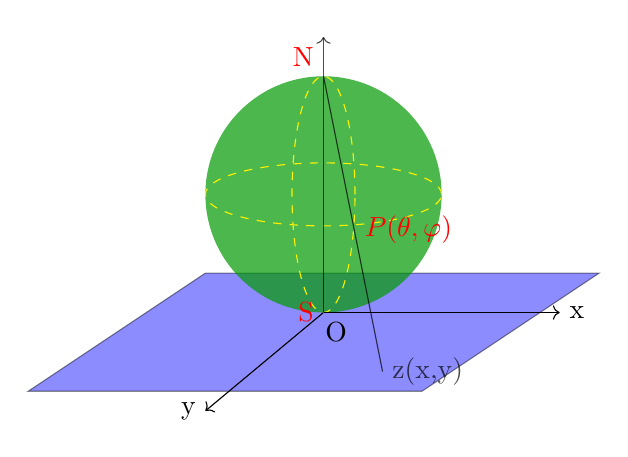
\begin{tikzpicture}[scale=0.5]
    \draw[xslant=1.5, fill=blue, opacity=0.45]
    (0,-5) rectangle (10,-2);
    \node (Center) at (0,0) {};
    \fill[green!60!black, opacity=0.7] (Center) circle (3cm);
    \draw[dashed,draw=yellow ] (Center)  ellipse (3cm and 0.8cm);
    \draw[dashed,draw=yellow ] (Center)  ellipse (0.8cm and 3cm);
    \draw[->, opacity=0.7] (0,-3) -- (0,4) node[right] {};
    \draw[->] (0,-3) -- (-3,-5.5)  node[left] {y};
    \draw[->] (0,-3) -- (6,-3)  node[right] {x};
    \draw[opacity=0.7] (0,3) -- (1.5,-4.5)  node[right] {z(x,y)};
    \node [left,red] at (0,-3)   {S};
    \node [above left,red] at (0,3)   {N};
    \node [right,red] at (0.8,-0.9)   {$P(\theta,\varphi)$};
    \node [right] at (-0.2,-3.5)  {O};
\end{tikzpicture}  
\caption{复球面示意图}
    \label{fig:fqm}
\end{figure}
%\begin{figure}[htbp]
%    \centering
%    \includegraphics[width=0.38\textwidth]{figs/cn6.png}
%    \caption{复球面示意图}
%    \label{fig:fqm}
%\end{figure}
北极$N$与复平面点$z(x,y)$的连线与球面交于点$P(\theta, \varphi)$。很明显,通过这种连线,球面上的点与复平面的点构成一一对应关系。特别地,球面的北极$N$是复平面无穷大$\infty$的几何表示。这样,球面上的每一点都有唯一的一个复数与之对应,因此称为\emph{复球面}。并称点$P(\theta, \varphi)$为复数$z$的\emph{复球面表示}。
\begin{equation}
    z = P(\theta, \varphi)
\end{equation}
包括无穷远点在内的复平面称为\emph{扩充复平面}。不包括无穷远点在内的复平面称为\emph{有限复平面}, 简称复平面。

对于复数$\infty$,它的模规定为正无穷大, 而实部,虚部和辐角等概念均无意义。很明显,复球面表示的优越性在于能把复数$\infty$(或者说复平面无穷远点)显式地表示出来。 对于复数$\infty$,有如下计算规则:
\begin{compactitem}
    \item 加法: $z + \infty = \infty +z = \infty, \quad ( z \ne \infty)$
    \item 减法: $z - \infty = \infty -z = \infty, \quad ( z \ne \infty)$
    \item 乘法: $z \cdot \infty = \infty \cdot z = \infty, \quad ( z \ne 0)$
    \item 除法: $\dfrac{z}{\infty} =0, \, \quad  \dfrac{\infty}{z} =\infty,(z \ne \infty ), \, \quad \dfrac{z}{0} =\infty, (z \ne 0)$
\end{compactitem}

~\\
\begin{hint}
    为适应不同问题的讨论, 复数有六种常见表示:
    \begin{compactitem}
      \item 代数表示 $~ z=x+yi$
      \item 向量表示 $~ z= \overrightarrow{oz}$ 
      \item 三角表示  $~ z=r (\cos \theta + i\sin \theta)$
      \item 指数表示  $~ z= r e^{i \theta}$
      \item 有序实数对表示  $~ z=(x,y)= (r\cos \theta, r\sin \theta )$
      \item 复球面表示 $~ z= P(\theta, \varphi)$
    \end{compactitem}
    它们各有其便, 且可相互转换。具体使用时以直观和方便计算为要。 
\end{hint}
\begin{example}
    试把复数$z=1-i$转化成指数形式。
\end{example}
\emph{解: } 可经三角式过渡
\[ \begin{aligned} 
    z&= \sqrt{2} (\frac{\sqrt{2} }{2} - i\frac{\sqrt{2} }{2}) \\
     &= \sqrt{2} (\cos \frac{1}{4}\pi - i\sin \frac{1}{4}\pi  ) \\
     &= \sqrt{2} [\cos (-\frac{1}{4}\pi) + i\sin (-\frac{1}{4}\pi  )]\\
     &= \sqrt{2}  e^{-i \frac{\pi}{4}} 
\end{aligned}\]
\begin{example}
    试把复数$z=1-\cos \theta + i \sin \theta \quad (0 < \theta \le \pi)$化成指数形式。
\end{example}
\emph{解: }由三角函数公式
\[ \begin{aligned} 
    z&= 1-\cos \theta + i \sin \theta \\
     &= 2 \sin ^2 \frac{\theta}{2}  + 2i \sin \frac{\theta}{2} \cos \frac{\theta}{2}\\
     &= 2 \sin \frac{\theta}{2}  (\sin \frac{\theta}{2}  +  i\cos \frac{\theta}{2} ) \\
     &= 2  \sin \frac{\theta}{2} [ \cos ( \frac{\pi}{2} -\frac{\theta}{2}) + i\sin ( \frac{\pi}{2} -\frac{\theta}{2}) ] \\
     &= 2\sin \frac{\theta}{2} e^{i (\pi-\theta) /2}
\end{aligned}\]

\subsection{复数的运算} ~\\

由于实数是复数的特例, 规定复数的运算法则时应满足一个基本要求,即:复数运算的法则施行于实数时, 应与实数运算的结果相符。同时,复数域是实数域的扩展,复数按新的法则运算时能够满足实数运算的一般定律,比如加法的交换律、结合律,乘法的交换律、结合律和乘法对加法的分配律等。\\

\noindent \emph{复数相等: } 

如果两复数在复平面上对应的点是同一点,则它们相等。
设复数
\[z_1 = (x_1,\, y_1) \qquad z_2=(x_2,\,y_2) \]
则它们相等时,其实部和虚部分别相等
\begin{equation}\label{} 
    {z}_{1}={z}_{2} \quad \Leftrightarrow \quad x_{1}=x_{2}, y_{1}=y_2
\end{equation}
设复数
\[z_1 = r_1 e^{i \theta_1} \qquad z_1 = r_2 e^{i \theta_2} \]
则它们相等时,其模长相等而辐角相差$2\pi$的整数倍
\begin{equation}\label{}
    {z}_{1}= {z}_{2} \quad  \Leftrightarrow \quad  r_1= r_2, \theta_1=2k \pi + \theta_2, \quad k \in \mathbb{Z}   
\end{equation}

\begin{proposition}\label{}
	与实数不同,复数只能判断是否相等,不能比较大小。或者说,只有两个复数同时为实数这种特殊情况下,才能比较大小。
\end{proposition}
\begin{proof}
	设虚数$i$可以和$0$比较大小, 则
\begin{compactitem}
   \item 由复数相等条件,可知 $i \ne 0$
   \item 若 $i>0$, 则 $ -1 = i\cdot i >  0 \cdot i  =0$, 矛盾!
   \item 若 $i<0$, 则 $-i> 0$, 因此 $ -1 = (-i)\cdot (-i) >  0 \cdot 0  =0$, 矛盾!
\end{compactitem}
因此,当两个复数不同时为实数时,不能比较大小。 
\end{proof}

\noindent \emph{复数加法: } 

把复数用向量表示,由向量加法得两复数加法法则,即:两复数的和等于它们的实部和虚部分别相加,如图[\ref{fig:fsjjf}]所示。
  \begin{equation}\label{}
      \begin{aligned}
     z &= z_1 + z_2  \\ 
     &= (x_1, y_1) + (x_2,y_2) \\
     &= (x_1+ x_2,\,  y_1+ y_2) 
    \end{aligned} 
  \end{equation}
  交换律
  \[ z_1 + z_2  = z_2 + z_1 \]
  结合律
  \[ (z_1 + z_2) + z_3  = z_1 +(z_2 + z_3) \]
  \begin{figure}[h]
    \centering
    \begin{minipage}[t]{0.49\textwidth}
        \centering
        \begin{tikzpicture}
            \tikzset{
                %Define standard arrow tip
                >=stealth',
                % Define arrow style
                pil/.style={->,thick}
                }
            \draw[thick,->] (-.5,0) -- (3.5,0) node[anchor=north west] {x};
            \draw[thick,->] (0,-.5) -- (0,3.5) node[anchor=north east] {y};
            \node[anchor=north east] at (0,0) {O};
            \draw[black!60!green,thick,->] (0,0) -- (2,0.5) node[right] {$z_1$};
            \draw[black!60!green,thick,->] (0,0) -- (0.5,2) node[right] at (0.5,1.9) {$z_2$};
            \draw[black!60!green,thick,->] (0,0) -- (2.5,2.5) node[right] {$z_1+z_2$};
            \draw[black!60!green,thick,dashed] (2.5,2.5) -- (2.5,0)  node[below] at (2.8,0) {$x_1+x_2$};
            \draw[black!60!green,thick,dashed] (2.5,2.5) -- (0,2.5)  node[left] {$y_1+y_2$};
            \draw[black!60!green,thick,dashed] (2,0.5) -- (2.0,0)  node[below] {$x_1$};
            \draw[black!60!green,thick,dashed] (2,0.5) -- (0,0.5)  node[left] {$y_1$};
            \draw[black!60!green,thick,dashed] (0.5,2) -- (0,2.0)  node[left] {$y_2$};
            \draw[black!60!green,thick,dashed] (0.5,2) -- (0.5,0)  node[below] {$x_2$};
            \draw[black!60!green,thick] (0.5,2) -- (2.5,2.5);
            \draw[black!60!green,thick] (2,0.5) -- (2.5,2.5);
        \end{tikzpicture}
        \caption{复数加法}
        \label{fig:fsjjf}
    \end{minipage}
    \begin{minipage}[t]{0.49\textwidth}
        \centering
        \begin{tikzpicture}
            \tikzset{
                %Define standard arrow tip
                >=stealth',
                % Define arrow style
                pil/.style={->,thick}
                }
                \draw[thick,->] (-.5,0) -- (3.5,0) node[anchor=north west] {x};
                \draw[thick,->] (0,-2.0) -- (0,2.0) node[anchor=north east] {y};
                \node[anchor=north east] at (0,0) {O};
                \draw[black!60!green,thick,->] (0,0) -- (-0.5,1.5) node[left] {$z_2$};
                \draw[black!60!green,thick,->] (0,0) -- (0.5,-1.5) node[below] {$-z_2$};
                \draw[black!60!green,thick,->] (0,0) -- (2,0.5) node[right] {$z_1$};
                \draw[black!60!green,thick,->] (0,0) -- (2.5,-1) node[right] {$z_1-z_2$};
                \draw[black!60!green,thick] (0.5,-1.5) -- (2.5,-1);
            \draw[black!60!green,thick] (2,0.5) -- (2.5,-1);
        \end{tikzpicture}
        \caption{复数减法}
        \label{fig:fsjjf2}
    \end{minipage}
 \end{figure}
%\begin{figure}[htbp]
%    \centering
%   \includegraphics[width=0.85\textwidth]{figs/cn1.png}
%    \caption{(a)复数的加法,(b)复数减法}
%    \label{fig:fsjjf}
%\end{figure}
\begin{corollary}\label{}
    \noindent 当有$n$个复数相加时
    \begin{equation}\label{} z_1 + z_2  + \cdots + z_n = (\sum_{j=1}^n x_j,\, \sum_{j=1}^n y_i)   
    \end{equation}
\end{corollary}

~\\
\noindent \emph{复数减法: }

减法是加法的逆。取$z_2$ 关于原点的对称点,即得$-z_2$,如图[\ref{fig:fsjjf2}]所示。得复数复数减法法则:
\begin{equation}\label{}
    z_1 - z_2 = z_1 +(-z_2) = (x_1 - x_2, y_1 - y_2) 
\end{equation}
即:两复数的差等于它们的实部和虚部分别做差。
两复数做差,在复平面上对应两个向量$\overrightarrow{z_1 z_2} = z_2 -z_1$ 和 $\overrightarrow{z_2 z_1} = z_1 -z_2$。它们的模相等,方向相反。 

~\\
利用测距算符
\begin{equation}\label{}
    \begin{aligned}
        \hat{d}[z_1, z_2] &= \left\vert z_1 - z_2\right\vert \\
            &=  \left\vert (x_1-x_2, \, y_1-y_2)\right\vert \\
            &= \sqrt{(x_1-x_2)^2 + (y_1-y_2)^2}  
        \end{aligned} 
\end{equation}
因此复数差的模具有复平面两点距离的几何意义, 
若取$z_2 =0$, $z =z_1$, 则有
        \[\left\vert z\right\vert = \hat{d}[z, 0] =  \left\vert \overrightarrow{oz}\right\vert\]
正如前所述,复数$z$的模就是向量$\overrightarrow{oz}$的长度。

~\\
由复数的和差公式,可得三角不等式:
\begin{equation}\label{}
    \begin{aligned}
        (1) &\quad   \left\vert z_1 + z_2 \right\vert \le \left\vert z_1 \right\vert +
        \left\vert z_2 \right\vert \\
        (2) &\quad  |z_1-z_2| \ge |z_1|  - |z_2|  \\
     (3) & \quad  |z_1-z_2| \le |z_1- z|  + |z-z_2|  \\ 
     (4) & \quad \left\vert \left\vert z_1\right\vert - \left\vert z_2\right\vert \right\vert  \le \left\vert z_1 \pm z_2 \right\vert 
     \le \left\vert z_1\right\vert + \left\vert z_2 \right\vert 
\end{aligned} 
\end{equation}
\begin{example}
    试证明不等式
    \[|z_1 -z_2| \ge ||z_1| - |z_2||\]
    \end{example}
\begin{proof}
    设原点$O$与点$z_1$、$z_2$不共线,则它们构成$\Delta Oz_1z_2$。此三角形的边长分别为
    $$a_1 =|z_1 -z_2|, \quad a_2 =|z_1|, \quad a_3 =|z_3|$$
    由于三角形两边长之差小于第三边边长, 因此有 
    \[|z_1 -z_2| > ||z_1| - |z_2||\]
    当三点共线时,有 
    \[|z_1 -z_2| = ||z_1| - |z_2||\]
    原不等式得证。
\end{proof}
\begin{corollary}\label{}
    \noindent 对于n个复数的和,存在不等式
    \begin{equation}
        |z_1 + z_2 + \cdots + z_n| \le |z_1| + |z_2| + \cdots +   |z_n| 
    \end{equation}
\end{corollary}
\begin{example}
    已知$x$是实数,求 
    \[f(x) = \sqrt{(x+4)^2 +4} - \sqrt{x^2 +1}\]
    的极大值
\end{example}
    \emph{解:} 令$z_1 = x+4 + 2i, \quad z_2 = x+i$,则有 
    \[ \begin{aligned}
        f(x) = |z_1| - |z_2| 
          \le |z_1-z_2| 
          = |x+4 + 2i - x -i| 
          = \sqrt{17}
    \end{aligned} \]
    取极值的条件为
    \[ \frac{2}{x+4} = \frac{1}{x}\]
    即$x=4$
\begin{example}
    求复数方程 
    \[\left\vert z+i\right\vert =2\]
    所表示的曲线 
    \end{example}
    \emph{解:} 做简单变换
    \[ \begin{aligned}
       \left\vert z+i\right\vert &=2  \\ 
       \left\vert z- (0-i)\right\vert &=2  \\ 
    \end{aligned} \]
    由测距算符可知,上式描述到定点$(0, -1)$的距离恒为 2 的点的集合,即此复数方程表示复平面上以点$(0, -1)$为圆心半径为2的圆线, 如图[\ref{fig:fbmyx}]所示。
    \begin{figure}[h]
		\centering
        \begin{minipage}[t]{0.49\textwidth}
            \centering
            \begin{tikzpicture}[scale=0.8]
                \tikzset{
                    %Define standard arrow tip
                    >=stealth',
                    % Define arrow style
                    pil/.style={->,thick}
                    }
                \draw[thick,->] (-2.5,0) -- (2.5,0) node[anchor=north west] {x};
                \draw[thick,->] (0,-3.5) -- (0,1.5) node[anchor=north east] {y};
                \node[anchor=north east] at (0,0) {O};
                \draw[black!60!green,thick,name path=l1]  (0,-1) circle (2); 
                \node[right] at(1.2,1.2) {$\left\vert z+i\right\vert =2$};
                \fill[]  (0,-1) circle (2pt); 
                \draw[white,thick,name path=l2]  (0,-1) -- (2,1); 
                \fill[name intersections = {of=l1 and l2,
            name=p}] (p-1) circle (1pt) node [above right] {};
             \draw[black!60!green,thick]  (0,-1) -- (p-1); 
            \end{tikzpicture}
            \caption{复平面圆线}
            \label{fig:fbmyx}
        \end{minipage}
        \begin{minipage}[t]{0.49\textwidth}
            \centering
            \begin{tikzpicture}[scale=1]
                \tikzset{
                    %Define standard arrow tip
                    >=stealth',
                    % Define arrow style
                    pil/.style={->,thick}
                    }
                \draw[thick,->] (-.5,0) -- (3.5,0) node[anchor=north west] {x};
                \draw[thick,->] (0,-.5) -- (0,3.5) node[anchor=north east]  {y};
                \node[anchor=north east] at (0,0) {O};
                \draw[black!60!green,thick,name path=l3] (-0.5,2.5) node[anchor=north] {$z_1$} -- (2.5,0.5) node[anchor=north] {$z_2$};
                \fill[black!60!green]  (-0.5,2.5)  circle (2pt); 
                \fill[black!60!green]  (2.5,0.5) circle (2pt); 
                \draw[white,thick,name path=l4] (0,0) -- (2,2) ;
                \fill[name intersections = {of=l3 and l4, name=p}] (p-1) circle (1pt) node [above right] {};
                \draw[black!60!green,thick]  (0,0) -- (p-1) node [above right] {z}; 
            \end{tikzpicture}
            \caption{复平面线段}
		    \label{fig:fpmxd}
        \end{minipage}
	 \end{figure}

    \begin{example}
        设$z_1, z_2$是复平面两点,试给出下列方程所描述的曲线
        \[ z= z_1 + t (z_2 - z_1), \qquad (0\le t\le 1)\]
    \end{example}
    \emph{解:} 变形,得 
    \[ z -z_1 = t (z_2 - z_1)\]
    向量 $\overrightarrow{z_1 z}$ 与向量 $\overrightarrow{z_1 z_2}$ 共点同向,即$z$点落在由线段$z_1z_2$确定的直线上。参量$t$的取值范围为$(0\le t\le 1)$,因此$z$描述线段$z_1z_2$上的任意点,即方程描述线段$z_1z_2$, 如图[\ref{fig:fpmxd}]所示。

    若改变参量$t$的取值范围: 
    \begin{equation}
        z= z_1 + t (z_2 - z_1), \qquad (-\infty < t < +\infty)
    \end{equation}
则方程描述由$z_1$和$z_2$点确定的直线,并称为复平面上两点确定直线的参数方程。\\
    
\noindent \emph{复数乘法: } 

根据虚数单位运算的约定,得虚数单位$i$的乘法法则:
\[\begin{aligned}
     {i}^1 &= i = (0,1) = e^{i \frac{\pi}{2}}\\
    {i}^2 &= -1 = (-1,0)= e^{i \pi} \\
     {i}^3 &= -i = (0,-1) = e^{i \frac{3\pi}{2}} \\
    {i}^4 &= 1 = (1,0) = e^{i 2\pi }\\ 
\end{aligned} \]
实现的是轴线上四点之间的跳转。因此,$i$的乘法存在周期性
\begin{equation}\label{}
    \begin{aligned}
     i^{4 k}=1,\quad 
     i^{4 k+1}=i,\quad 
     i^{4 k+2}=-1 ,\quad 
     i^{4 k+3}=-i  \qquad (k \in \mathbb{Z}^+)
\end{aligned} 
\end{equation}
数乘
\begin{equation}\label{}
    \begin{aligned}
    i z &= (-y, x) \\
    c z &= (cx, cy)  \\
    ic z &= (-cy, cx) \qquad c \in \mathbb{R}
\end{aligned} 
\end{equation}
复数乘
\begin{equation}\label{}
    \begin{aligned}
    z &= z_1 z_2  \\ 
    &= (x_1, y_1) (x_2,y_2) \\
    &= (x_1x_2- y_1y_2,\,  x_1y_2+x_2y_1) 
   \end{aligned}  
\end{equation}
   交换律
   \[ z_1 z_2  = z_2 z_1 \]
   结合律
   \[ (z_1 z_2)z_3  = z_1 (z_2 z_3) \]
   分配律
   \[ z_1 (z_2 + z_3)  = z_1 z_2 + z_1 z_3\]
采用极坐标表示复数乘法
	\[z= z_1 z_2 = r_{1} e^{\boldsymbol{i}\theta_{1}} \times r_{2} e^{\boldsymbol{i}\theta_{2}} = r_{1} r_{2} e^{\boldsymbol{i}\theta_{1}} e^{\boldsymbol{i}\theta_{2}}\]
    计算后两项的积
    \[ \begin{aligned}
		e^{\boldsymbol{i}\theta_{1}} e^{\boldsymbol{i}\theta_{2}} &=
\left(\operatorname{cos}\left[\theta_{1}\right]+i \operatorname{sin}\left[\theta_{1}\right]\right)\left(\operatorname{cos}\left[\theta_{2}\right]+i \operatorname{sin}\left[\theta_{2}\right]\right) \\
		& =\left(\operatorname{cos}\left[\theta_{1}\right] \operatorname{cos}\left[\theta_{2}\right]-\operatorname{sin}\left[\theta_{1}\right] \operatorname{sin}\left[\theta_{2}\right]+i\left(\operatorname{sin}\left[\theta_{1}\right] \operatorname{cos}\left[\theta_{2}\right]+\operatorname{cos}\left[\theta_{1}\right] \operatorname{sin}\left[\theta_{2}\right]\right)\right) \\
		& =\left(\operatorname{cos}\left[\theta_{1}+\theta_{2}\right]+i \operatorname{sin}\left[\theta_{1}+\theta_{2}\right]\right) \\
		& = e^{\boldsymbol{i}\left(\theta_{1}+\theta_{2}\right)}
		\end{aligned} \]
   得乘法公式 
   \begin{equation}\label{}
       z_1 z_2 = r_{1} r_{2} e^{\boldsymbol{i}\left(\theta_{1}+\theta_{2}\right)} 
   \end{equation}
   分析:
   \[ \begin{aligned}
       \begin{aligned}
           z &= z_2z_1  \\
           &= r_{2} e^{\boldsymbol{i}\theta_{2}} z_1  \\ 
           &= r_{2} [\hat{R}(\theta_{2})z_1] \\
       \end{aligned} 
   \end{aligned}\]
   复数乘法的几何意义:先把$z_1$逆时钟旋转$\theta_2$角,然后把其模伸缩$r_2$倍,如图[\ref{fig:fstimes}]所示。
   \begin{figure}[h]
    \centering
            \begin{tikzpicture}[scale=1]
                \tikzset{
                    %Define standard arrow tip
                    >=stealth',
                    % Define arrow style
                    pil/.style={->,thick}
                    }
                \draw[thick,->] (-.5,0) -- (3.5,0) node[anchor=north west] {$x$};
                \draw[thick,->] (0,-.5) -- (0,3.5) node[anchor=north east]  {$y$};
                \node[anchor=north east] at (0,0) {O};
                % angle \theta_1
                \draw[fill=blue!10] (0,0) -- (0:0.95cm) arc (0:27:.95cm);
                \draw[black!60!green,thick]  (1.15cm,0.15cm) node {$\theta_1$};
                % angle \theta_2
                \draw[fill=blue!20] (0,0) -- (0:0.60cm) arc (0:44:.60cm);
                \draw[black!60!green,thick]  (0.72cm,0.3cm) node {$\theta_2$};
                 % angle \theta
                 \draw[fill=blue!50] (0,0) -- (0:0.35cm) arc (0:73:.35cm);
                 \draw[black!60!green,thick]  (0.3cm,0.47cm) node {$\theta$};
                \draw[black!60!green,thick, ->,name path=l5] (0,0) -- (2,1)  node[right]{$z_1$};
                \draw[black!60!green,thick, ->,name path=l5] (0,0) -- (1.5,1.5)  node[right]{$z_2$}; 
                \draw[black!60!green,thick, ->,name path=l5] (0,0) -- (1.1,3.0) node[right] {$z = z_1 z_2$}; 
            \end{tikzpicture}
    \caption{复数乘法}
    \label{fig:fstimes}
\end{figure}

\begin{corollary}\label{} n个复数的乘法
    \begin{equation}\label{}
        z_1z_2\cdots z_n = (\prod\limits_{j=1}^{n}r_j) \boldsymbol{e}^{\boldsymbol{i} \sum _{j=1}^{n} \theta _j } 
    \end{equation}
\end{corollary}

\begin{corollary}\label{} 复数的乘幂
    \begin{equation}\label{eq:fscft2}
        \begin{aligned}
      z^n &=  r^n e^{i n \theta}\\ 
      &=  r^n (\cos n \theta + i \sin n \theta) , \qquad n \in \mathbb{Z}^+ 
      \end{aligned} 
    \end{equation}
\end{corollary}
\begin{hint}
很明显,复数的乘法既不是向量的点积, 也不是向量的叉积。
\end{hint}

\begin{example}
    设物体受四个力的作用,如图[\ref{fig:fsmsjf}]所示, \\
\begin{figure}[h]
    \centering
    \begin{tikzpicture}[scale=0.6]
        \tikzset{
            %Define standard arrow tip
            >=stealth',
            % Define arrow style
            pil/.style={->,thick}
            }
        \draw[thick,->] (-3.5,0) -- (3.5,0) node[anchor=north west] {$x$};
        \draw[thick,->] (0,-.5) -- (0,4.5) node[anchor=north east]  {$y$};
        \node[anchor=north east] at (0,0) {O};
        \draw[black!60!green,thick,->] (0,0) -- (2.5, 1) node[right]  {$F_1(2.5,1)$};
        \draw[black!60!green,thick,->] (0,0) -- (1, 3) node[right]  {$F_2(1,3)$};
        \draw[black!60!green,thick,->] (0,0) -- (-1, 4) node[left]  {$F_3(-1,4)$};
        \draw[black!60!green,thick,->] (0,0) -- (-3, 1.5) node[left]  {$F_3(-3,1.5)$};
    \end{tikzpicture}
        \caption{复数描述的力}
        \label{fig:fsmsjf}
\end{figure}
%\begin{figure}[h]
%       \centering
%       \includegraphics[width=0.35\textwidth]{figs/c-9.png}
%       \caption{复数描述的力}
%      \label{fig:fsmsjf}
%\end{figure}
试求:
\begin{inparaenum}[(1)]
    \item 合外力的大小和方向,
    \item 若$F_2$逆时针旋转45度, 合外力的大小和方向。
\end{inparaenum}

\end{example}
\emph{解:} (1) 把力写成复数形式, 计算合力 
\[ \begin{aligned}
   F &= (2.5 +1-1-3, 1+3+4+1.5) \\ 
   &= (-0.5, 9.5)
\end{aligned} \]
大小: $\left\vert F\right\vert = \sqrt{0.5^2 + 9.5^2} =9.51 $ \\
方向:$\theta = \arg F + \pi = \pi - \text{argtan} \dfrac{9.5}{0.5}  = \pi - \text{argtan} (19)$ \\
(2) $F_2$逆时针旋转45度
\[ \begin{aligned}
  F'_2 &= \hat{R}(\frac{\pi}{4})(1,3) \\
  &= (1, 1) \cdot (1,3) \\ 
  &= (-2, 4)
\end{aligned}\]
计算合力 
\[ \begin{aligned}
   F &= (2.5 -2-1-3, 1+4+4+1.5) \\ 
   &= (-3.5, 10.5)
\end{aligned} \]
大小: $\left\vert F\right\vert = \sqrt{3.5^2 + 10.5^2} =11.07 $ \\
方向:$\theta = \arg F + \pi = \pi - \text{argtan} \dfrac{10.5}{3.5}  = \pi - \text{argtan} (3)$ \\

\noindent \emph{共轭运算: } 

\begin{example}
    在复平面找点$z$关于$x$轴的对称点$z^*$。
    \begin{figure}[h]
        \centering
        \begin{tikzpicture}[scale=1]
        \tikzset{
        %Define standard arrow tip
         >=stealth',
        % Define arrow style
        pil/.style={->,thick}
        }
                    \draw[thick,->] (-.5,0) -- (4.5,0) node[anchor=north west] {};
                    \draw[thick,->] (0,-2.0) -- (0,2.0) node[anchor=north east] {};
                    \node[anchor=north east] at (0,0) {O};
                    % angle \theta
                    \draw[fill=blue!20] (0,0) -- (0:0.60cm) arc (0:44:.60cm);
                    \draw[black!60!green,thick]  (0.72cm,0.3cm) node {$\theta$};
                    % angle -\theta
                    \draw[fill=blue!20] (0,0) -- (0:0.60cm) arc (0:-44:.60cm);
                    \draw[black!60!green,thick]  (0.72cm,-0.3cm) node {$-\theta$};
                    \draw[black!60!green,thick,->] (0,0) -- (1.5,1.5)  node[right]{$z$}; 
                    \draw[black!60!green,thick,->] (0,0) -- (1.5,-1.5)  node[right]{$z^*$}; 
                    \draw[black!60!green,thick,dashed] (1.5,1.5) -- (0,1.5)  node[left]{$y$}; 
                    \draw[black!60!green,thick,dashed] (1.5,-1.5) -- (0,-1.5)  node[left]{$-y$}; 
                    \draw[black!60!green,thick,dashed] (1.5,1.5) -- (1.5,0) node[right] at (1.5,-0.2) {$x$}; 
                    \draw[black!60!green,thick,dashed] (1.5,-1.5) -- (1.5,0) ; 
                    \draw[black!60!green,thick,->] (0,0) -- (3,0)  node[above] at (3.3,0) {$z+z^*$};
                    \draw[black!60!green,thick] (1.5,-1.5) -- (3,0) ;
                    \draw[black!60!green,thick] (1.5,1.5) -- (3,0) ;
                    \draw[black!60!green,thick,->] (0,0) -- (4,0)  node[below] {$zz^*$};
                \end{tikzpicture}
        %\includegraphics[width=0.2\textwidth]{figs/c-3.png}
        \caption{共轭复数}
        \label{fig:gefs}
    \end{figure} 
\end{example}
很明显
  \begin{equation}\label{}
       z=(x, \, y ),  \qquad z^* = (x, \, -y)   
  \end{equation}
指数形式
  \begin{equation}\label{}
    z= r e^{i \theta}, \qquad  z^*= r e^{-i \theta}
\end{equation}  
我们把实部相同而虚部互为相反数的两个复数称为\emph{共轭复数 },比如: $z^*$与$z$互为共轭复数。
通常也称$z^*$为$z$的共轭复数,记为:$\overline{z} = z^*$, 如图[\ref{fig:gefs}]所示。共轭复数具有如下运算性质:
\begin{equation}\label{}
    \begin{aligned}
    &(1) \, \overline{z_{1} \pm z_{2}}=\bar{z}_{1} \pm \bar{z}_{2} \qquad  (z_{1} \pm z_{2})^* = z_{1}^* \pm z_{2}^* \\
    &(2) \, \overline{z_{1} \cdot z_{2}}=\bar{z}_{1} \cdot \bar{z}_{2}  \hspace{1em} \qquad (z_{1} \cdot z_{2})^* = z_{1}^* \cdot z_{2}^* \\
    &(3) \, \overline{\left(\frac{z_{1}}{z_{2}}\right)}=\frac{\bar{z}_{1}}{\bar{z}_{2}}  \hspace{2em} \qquad \left(\frac{z_{1}}{z_{2}}\right)^* = \frac{z_{1}^*}{z_{2}^*}\\
    &(4) \,\bar{\bar{z}}=z \hspace{5em} \qquad  (z^*)^* = z \\
    &(5) \,z \cdot \bar{z}=\left\vert z\right\vert^2 \hspace{3em} \qquad  z \cdot z^* = \left\vert z\right\vert^2 \\
    &(6) \,z+\bar{z}=2 \operatorname{Re}(z)  \hspace{1em} \qquad  z+z^*=2 \operatorname{Re}(z)  \\
    &(7) \,z-\bar{z}=2 i \operatorname{Im}(z)  \hspace{0.5em} \qquad z-z^*=2 i \operatorname{Im}(z) \\ 
\end{aligned} 
\end{equation}

注意到$z+z^*$和$zz^*$总是实数,而$z-z^*$通常是纯虚数。灵活运用这些公式,可提高复数计算的效率。
\begin{example}
    设$z_1 $ ,$ z_2 $ 是两个任意复数, 试证明 
	\[ \left\vert z_1 + z_2\right\vert ^2 =  \left\vert z_1\right\vert^2 + \left\vert z_2\right\vert^2  + 2 Re(z_1z_2^*)\] 
\end{example}
\begin{proof}
    由模方公式 
	\[ \begin{aligned}
		\left\vert z_1 + z_2\right\vert ^2  &= (z_1 + z_2)(z_1 + z_2)^* \\ 
		&= (z_1 + z_2)(z_1^* + z_2^* ) \\
		&= z_1 z_1^* + z_2 z_2^*  + z_1 z_2^* + z_1^* z_2  \\
		&= z_1 z_1^* + z_2 z_2^* + z_1 z_2^* + (z_1 z_2^*)^*  \\
		&= \left\vert z_1 \right\vert^2 + \left\vert z_2 \right\vert^2 + 2 Re(z_1z_2^*)
	\end{aligned}\]
\end{proof}

\noindent \emph{复数除法: } 

除法是乘法的逆, 对于$z= 1 \cdot z = r e^{i\theta}$,它是由实数单位"1"逆时针旋转$\theta$角后其模再伸缩r倍而来,则$\dfrac{1}{z}$应能把$z$逆变成实数单位"1",即 
\[ \frac{z}{z} = z \cdot \frac{1}{z}  = r e^{i\theta} \cdot \frac{1}{z}   =1 \]
可得
\begin{equation}\label{}
    \frac{1}{z} = \frac{1}{r} e^{i(- \theta)}  = \frac{1}{r} [\cos(-\theta) + i \sin(- \theta)]
\end{equation}
当$z_2 \ne 0$时,有 
\begin{equation}\label{}
    \begin{aligned}
    \frac{z_1}{z_2} &=  \frac{z_1 z^*_2 }{|z_2|^2 }  \\ 
    &= \frac{(x_1, y_1)(x_2, -y_2) }{x^2_2+ y^2_2}   \\
    &= \frac{(x_1x_2 + y_1y_2, x_2y_1 -x_1y_2)}{x^2_2+ y^2_2}   
\end{aligned} 
\end{equation}
极坐标形式
\begin{equation}\label{}
      z = \frac{z_1}{z_2} = \frac{r_1}{r_2} e^{i(\theta _1 - \theta _2)}  
\end{equation}
除法的几何意义:先把$z_1$顺时钟旋转$\theta_2$角,然后再把模伸缩$\dfrac{1}{r_2}$倍。\\
\begin{example}
    已知
	\[ z_1 = \frac{1}{2}(1-i\sqrt{3}), \, z_2 = \sin \frac{\pi}{3} -i \cos \frac{\pi}{3}\]
	求$z_1z_2$ 和 $\dfrac{z_1}{z_2}$
\end{example}
\emph{解: } 把 $z_1, z_2$化成指数形式
\[ \begin{aligned}
    z_1 &= \cos (- \frac{\pi}{3}) + i  \sin  (- \frac{\pi}{3})  = e^{-i \pi /3}\\
    z_2 &= \cos (- \frac{\pi}{6}) + i  \sin  (- \frac{\pi}{6})  = e^{-i \pi /6}\\
\end{aligned}\]
代入乘法公式
\[ z_1 \cdot z_2 = e^{-i (\pi /3 +\pi /6) } = e^{-i \pi /2 } = -i\]
代入除法公式
\[ \dfrac{z_1}{z_2} = e^{i (-\pi /3 + \pi /6) } = e^{-i \pi /6 } \]
\begin{example}
    已知 
	\[ z_1 = \left( \frac{1-i}{1+i}\right)^7 + i, \, z_2 = \frac{i}{1-i} + \frac{1-i}{i}  + \frac{3}{2}\] 
	求 $z_1 \cdot z_2 $ 和$\dfrac{z_1}{z_2}$ 
\end{example}
\emph{解:}(1) 先求出$z_1$ 和$z_2$, 
\[ \begin{aligned}
    \frac{1-i}{1+i} &= \frac{(1-i)(1+i)^*}{|1+i|^2} = \frac{(1-i)^2}{2}  = -i 
\end{aligned}\]
因此
\[ z_1 = (-i)^7 + i = -(i)^3 + i = 2 i\]
由于
\[ \begin{aligned}
    \frac{i}{1-i} + \frac{1-i}{i} &= \frac{i(1+i)}{2} - (1-i)i  = - \frac{3}{2} - \frac{1}{2} i 
\end{aligned}\]
因此 
\[     z_2 = - \frac{3}{2} - \frac{1}{2} i  + \frac{3}{2} = - \frac{1}{2} i\]
(2) $z_1 \cdot z_2 $
\[ z_1 \cdot z_2 = - 2 i \cdot  \frac{1}{2} i =  1 \]
(3) $\dfrac{z_1}{z_2}$
\[ \frac{z_1}{z_2} = - \frac{2 i}{\frac{1}{2} i} = -4 \]
\begin{example}
    试证明平面三角形的内角和等于$\pi$
\end{example}
\begin{proof}
设三角形的三个顶点$z_1, z_2, z_3$对应的内角分别为$\alpha, \beta, \gamma$。则有
\[\alpha = \arg \frac{z_3-z_1}{z_2- z_1}, \, \beta = \arg \frac{z_3-z_2}{z_1- z_2}, \, \gamma = \arg \frac{z_1-z_3}{z_2- z_3}\] 
由于 
\[ \frac{z_3-z_1}{z_2- z_1} \cdot \frac{z_3-z_2}{z_1- z_2} \cdot \frac{z_1-z_3}{z_2- z_3} = -1\]
得
\[\arg \frac{z_3-z_1}{z_2- z_1} + \arg \frac{z_3-z_2}{z_1- z_2} + \arg \frac{z_1-z_3}{z_2- z_3} = \arg(-1) + 2 k \pi = \pi + 2 k \pi\] 
即  \[ \alpha + \beta + \gamma =  \pi + 2 k \pi, \quad \text{k为某适当整数}\] 
又由于$ 0< \alpha,  \beta, \gamma < \pi $,得
\[ 0< \alpha + \beta + \gamma < 3 \pi \]  
两式都成立,必有$k = 0 $, 故而 $\alpha + \beta + \gamma = \pi$
\end{proof}

\noindent \emph{复数的乘幂与方根: }

\noindent (1) 正整数幂 \\
作为乘积的特例, 我们考虑非零复数$z$的正整数次幂,由复数乘法推论[\ref{eq:fscft2}],可得复数乘幂公式的三角表示
\begin{equation}\label{}
    z^n =  r^n (\cos n \theta + i \sin n \theta) , \qquad n \in \mathbb{Z}^+  
\end{equation}
极坐标形式
\begin{equation}\label{}
    z^n =  r^n e^{i n \theta}
\end{equation}
存在性质
\begin{equation}\label{}
\begin{cases}
   \left\vert z^n\right\vert = \left\vert z\right\vert^n \\ 
   \text{Arg } z^n  = n \text{Arg }z
\end{cases}
\end{equation}
当$z$的模$r=1$时, 得\emph{棣莫佛公式 }
\begin{equation}\label{}
     (\cos \theta + i \sin  \theta)^n = \cos n \theta + i \sin n \theta
\end{equation}
~\\
\noindent (2) n-次方根 \\
	设 $z=|r| e^{i \theta }$是非零复数,它的n-次方根为$w = |w| e^{i \phi } $, 即
	\[ \begin{aligned}
		w^n &= z \\ 
		|w| ^n  e^{i n\phi } &= |z| e^{i \theta } 
	\end{aligned}\]
	计算模 
	\[ \begin{aligned}
		|w|^n  &= |z| \\ 
		|w| &= |z|^{\frac{1}{n}}
	\end{aligned}\]
	计算辐角
	\[ \begin{aligned}
		n\phi  &= 2 k \pi +\theta \\ 
		\phi  &= \frac{2 k \pi +\theta}{n} \quad (k=0,1,2,\cdots , n-1)
	\end{aligned}\]
    可得n个解
    \[ \begin{aligned}
     w_0 &= |z|^{\frac{1}{n}} e^{i \frac{\theta}{n}} \\ 
     w_1 &= |z|^{\frac{1}{n}} e^{i \frac{\theta}{n}} e^{i \frac{2\times 1\pi}{n}} = e^{i \frac{2\times1\pi}{n}} w_0  \\ 
     w_2 &= |z|^{\frac{1}{n}} e^{i \frac{\theta}{n}} e^{i \frac{2\times 2\pi}{n}} = e^{i \frac{2\times 2\pi}{n}} w_0  \\ 
     ~~ ~~ & \cdots\cdots\cdots   \\
     w_{n-1} &= e^{i \frac{2\times (n-1)\pi}{n}} w_0 
    \end{aligned}\]
    写在一起, 得n-次方根公式
    \begin{equation}\label{}
        \begin{aligned}
         w_k &= e^{i k\frac{2  \pi}{n}} w_0 \quad (k=0,1,2,\cdots , n-1) 
        \end{aligned} 
    \end{equation}
    令$\varphi = \dfrac{2  \pi}{n}$,则 
    \begin{equation}\label{}
        \begin{aligned}
         w_k = e^{i k \varphi} w_0 \quad (k=0,1,2,\cdots , n-1) 
           \end{aligned} 
    \end{equation}
    写成旋转算符形式
    \begin{equation}\label{}
        \begin{aligned}
               w_k = \hat{R}(k \varphi) w_0 \quad (k=0,1,2,\cdots , n-1)
           \end{aligned} 
    \end{equation}
    说明把$w_0 = |z|^{\frac{1}{n}} e^{i \frac{\theta}{n}} $逆时钟旋转$k$倍$\varphi= \dfrac{2  \pi}{n}$角,既得$w_k$。因此,$w_0, w_1,w_2,\cdots w_{n-1}$正好把$2 \pi$ 分为$n$等份。 
\begin{figure}[htbp]
    \centering
    \begin{tikzpicture}[scale = 2]
        \tikzset{
            %Define standard arrow tip
            >=stealth',
            }
        \draw[->] (-1.3,0) -- (1.3,0) node[below] {$x$}; %作x轴并标上字母
        \draw[->] (0,-1.3) -- (0,1.3) node[left] {$y$}; %作y轴并标上字母
        %\node[below left] at (0,0) {$O$}; %标上原点字母 
        \foreach \t in {0,60,120,180,240,300}{
            \draw[black!60!green,thick] (0,0) -- ({sin(\t +10)},{cos(\t +10)});}
        \draw[black!60!green,thick] ({sin(0 +10)},{cos(0 +10)}) node[above] {$w_1$}-- ({sin(60 +10)},{cos(60 +10)}) node[right] {$w_0$} -- ({sin(120 +10)},{cos(120 +10)}) node[right] {$w_5$} -- ({sin(180 +10)},{cos(180 +10)}) node[below] {$w_4$}  -- ({sin(240 +10)},{cos(240 +10)}) node[left] {$w_3$} -- ({sin(300 +10)},{cos(300 +10)}) node[left] {$w_2$}  -- ({sin(0 +10)},{cos(0 +10)}) ;
        \draw[thick] (0,0) circle(1);
        \draw[fill=blue!20] (0,0) -- (0:0.30cm) arc (0:20:.30cm);
        \draw[black!60!green,thick] (10:0.6cm) node {$\theta/6$};
       \end{tikzpicture}
    %\includegraphics[width=0.4\textwidth]{figs/c-6.png}
    \caption{复数$z$的6-次方根}
    \label{fig:scfg}
\end{figure}
~\\

例如:若取 $n=6$, 则 $ w_0 =  \left\vert z\right\vert ^{\frac{1}{6}} e^{i\frac{\theta}{6}}$, 并且 $\varphi = \dfrac{2  \pi}{6} = \dfrac{\pi}{3}$。取$k=1,2,\cdots ,5$, 然后把$ w_0 $旋转$ k \varphi $得其他五个解。这六个解是圆点在原点半径为$\left\vert z\right\vert ^{\frac{1}{6}} $的圆内接正六边形的顶点, 如图[\ref{fig:scfg}]所示。
    
若令$\omega = e^{i \frac{2 \pi}{n}}$, 有  $\omega^n =1$。则 $1$的$n$-次方根记为$1, \omega, \omega^2, \cdots, \omega^{n-1}$, 由它们在单位圆上的分布对称性,得公式 
    \begin{equation}
        1 + \omega + \omega^2 + \cdots + \omega^{n-1} =0  , \qquad  (\omega^n =1) 
    \end{equation}
特别地,当$n=3$时,有$\omega = e^{i \frac{2 \pi}{3}}  = - \dfrac{1}{2} + \dfrac{\sqrt{3}}{2} i $, 得 
    \begin{equation}
        1 + \omega + \omega^2 =0, \qquad  (\omega^3 =1) 
    \end{equation}
\begin{example}
    试把 $\cos 3\theta$ 分解成 $\cos \theta$ 的表达式 
\end{example}
\emph{解: }由棣莫弗公式
\[ \begin{aligned}
 z &= \cos 3 \theta + i \sin  3 \theta \\
    &= (\cos \theta + i \sin  \theta)^3 \\ 
    &= \cos ^3 \theta  + 3 i \cos ^2 \theta \sin \theta - 3 \cos \theta \sin ^2 \theta - i \sin ^3 \theta \\ 
    &= (\cos ^3 \theta - 3 \cos \theta \sin ^2 \theta ) + i (3  \cos ^2 \theta \sin \theta - \sin ^3 \theta )
\end{aligned}\]
因此有
\[\begin{aligned}
  \cos 3 \theta &=  \cos ^3 \theta - 3 \cos \theta \sin ^2 \theta  \\ 
  &= 4 \cos ^3 \theta - 3 \cos \theta
\end{aligned}\]
\begin{example}
    求$ \sqrt[3]{-8}$的根 
\end{example}
\emph{解:}把-8 写成复数的指数形式
\[ \begin{aligned}
     -8 &= 8 e^{i \pi}  \\ 
\end{aligned}\]
因此, 三次方根为 \[ w = \sqrt[3]{8} e^{i (2k +1)\pi / 3}, \, (k = 0, 1, 2) \]
代入,有
\[ \left\{ \begin{array} {rl}
    w_0 &= 2 e^{i \pi / 3} \\
    w_1 &= -2 \\
    w_2 &= 2 e^{-i \pi / 3}
\end{array} \right.\]
\begin{example}
解复数方程 
\[ (1+z)^5 = (1-z)^5\]
\end{example}
\emph{解:}把 $z=1$ 代入,方程不成立,说明 $z \ne 1$, 因此有 
\[ \begin{aligned}
    (1+z)^5 /(1-z)^5 &=  1 \\ 
    \left( \frac{1+z}{1-z}\right) ^5 &=1 \\
    w ^5 &= 1
\end{aligned}\]
由n-次方公式,有
\[ w = e^{i\frac{2k\pi}{5}} =  e^{i k\varphi\pi} , \quad (k=0,1,2,3,4)\]
 由于
 \[ \frac{1+z}{1-z}= w_k \]
 可得
 \[ \begin{aligned}   
   z &= \frac{w_k -1 }{w_k + 1} = \frac{e^{i k\varphi\pi} -1 }{e^{i k\varphi\pi} + 1}  \\ 
    &= \frac{\cos k \varphi + i \sin k \varphi -1 }{\cos k \varphi + i \sin k \varphi + 1}  \\ 
    &= \frac{2 \sin k\frac{\varphi}{2}\left(-\sin k\frac{\varphi}{2}+i \cos k\frac{\varphi}{2}\right)}{2 \cos k\frac{\varphi}{2}\left(\cos k\frac{\varphi}{2}+i \sin k\frac{\varphi}{2}\right)} \\
    &= i \tan k\frac{\varphi}{2} 
 \end{aligned}\]
 代入$\varphi = \dfrac{2k\pi}{5}, k=0,1,2,3,4 $, 得
 \[ z_0 = 0, z_1= i \tan \frac{\pi}{5} , z_2= i \tan \frac{2\pi}{5}, z_3 = i \tan \frac{3\pi}{5}, z_4 = i \tan \frac{4\pi}{5}\]
\begin{example}
 试证明:三个复数$z_1, z_2, z_3$ 在复平面构成等边三角形的充要条件为
 \[z^2_1 + z^2_2 + z^2_3  = z_1 z_2 + z_2 z_3 + z_3 z_1\]
\end{example}
\begin{proof}
若$\Delta z_1 z_2 z_3$ 是等边三角形,则向量$\overrightarrow{z_1 z_2}$绕$z_1$ 左旋转 $\pi/3$或右旋转 $\pi/3$必得向量$\overrightarrow{z_1 z_3}$
\[\begin{aligned}
    z_3 - z_1  &= (z_2 - z_1)e^{\pm \frac{\pi}{3} i} \\ 
    \frac{z_3 - z_1  }{z_2 - z_1}&= \cos \frac{\pi}{3} \pm i \sin \frac{\pi}{3} \\
    \frac{z_3 - z_1  }{z_2 - z_1} - \frac{1}{2}&= \pm \frac{\sqrt{3}}{2}  i \\
\end{aligned}\]
两边平方并化简,得 
\[z^2_1 + z^2_2 + z^2_3  = z_1 z_2 + z_2 z_3 + z_3 z_1\]
\end{proof}    


\section{复平面的点集}\label{sec:order}

在复数环节,我们已看到复平面上的线段、直线和圆周等都是复平面上的点的集合。复变函数的定义域和
值域通常是复平面上的点集。因此,我们有必要先了解复平面点集的基本概念及相关知识,然后再进入复变函数环节。

复平面的点集可以是由一个个相互孤立的点构成的集合,也可以是由一条直线、线段或一段曲线上的所有连续点构成的集合,也可以是由聚在某个区域内的所有连续点构成的集合。如果用点集所含点的多少来定义点集的大小,则复平面上任意点集$D$的大小记为$|D|$。多个点集的并集可以构成更大的点集,最大的点集是由复平面上所有的点构成的点集$\mathbb{C}$,并称$\mathbb{C}$为\emph{全集}。复平面上任意点集$D$都是全集$\mathbb{C}$的子集。

\subsection{平面点集的几个概念}

\begin{definition}\label{}\index{}
    设$z_0 \in \mathbb{C},  r  \in \mathbb{R} \mid  r  > 0$, 点集$\{z \mid \left\vert z - z_0 \right\vert <  r , z \in \mathbb{C} \}$ 称为$z_0$的$ r $-\emph{邻域}, 记为$U(z_0,  r )$, 其中$z_0$为邻域的中心,$ r $为邻域的半径。并称点集$\{z \mid 0 < \left\vert z - z_0 \right\vert <  r , z \in \mathbb{C} \}$为$z_0$的$ r $-\emph{去心邻域} 。
    \begin{figure}[htbp]
      \centering
      \includegraphics[width=0.9\textwidth]{figs/c-11.png}
      \caption{不等式与邻域:(a)邻域,(b)闭圆,(c)去心邻域 }
        %\label{fig:}
    \end{figure} 
\end{definition}
说明:
\begin{compactitem}
    \item 设 $M \in \mathbb{R} \mid M > 0$, 点集 $\{z \mid M<\left\vert z\right\vert  , z \in \mathbb{C} \}$ 是无穷远点的邻域,记为$U(\infty, M)$。点集 $\{z \mid M<\left\vert z\right\vert < + \infty , z \in \mathbb{C} \}$ 是无穷远点的去心邻域。
    \item 点集$\{z \mid \left\vert z - z_0 \right\vert <  r , z \in \mathbb{C} \}$ 是以$z_0$为圆心$ r $为半径的开圆, 是$z_0$的邻域。
    \item 点集$\{z \mid \left\vert z - z_0 \right\vert \le  r , z \in \mathbb{C} \}$ 是以$z_0$为圆心$ r $为半径的闭圆,不是$z_0$的邻域。
    \item 邻域概念是复数数列与复变函数极限的基础。
\end{compactitem}

\begin{definition}\label{}\index{}
	设点集$D \subset \mathbb{C}$, $z_0 \in \mathbb{C} $, $  r  \in \mathbb{R} \mid  r  > 0 $。 若 $ \forall |U(z_0,  r )\cap D| = \infty $, 则称$z_0$ 为$D$的\emph{聚点}或\emph{极限点}。点集$D$的所有聚点构成的集合记为$D^c$。若$\exists U(z_0,  r )\cap D = \{z_0 \}$, 则称$z_0$为$D$的\emph{孤立点}。
    \begin{figure}[htbp]
        \centering
        \includegraphics[width=0.9\textwidth]{figs/cn2.png}
        \caption{ (a) $z_0 \in D$,(b) $z_0 \notin D$但与$D$相邻,(c) $z_0 \notin D$也不与$D$相邻}
        \label{fig:jdjcd}
      \end{figure} 
\end{definition}
说明:
\begin{compactitem}
    \item 图[\ref{fig:jdjcd}]中 $r,p$取确定值时, 点集$D$确定。(a) $z_0$是$D$的聚点,(b) $z_0 \notin D$, 是点集$D$的聚点,(c)$z_0 \notin D$,不是$D$的聚点,也不是$D$的孤立点。        
    \item 若重新定义点集$D:\{ z_0, \left\vert z - p \right\vert <  r  \}$, 则(c)图的$z_0$依然不是$D$的聚点,但是却是$D$的孤立点。
    \item 孤立点不是聚点。
    \item 以下六种说法彼此等价:\\
    \begin{inparaenum}[(a)]
        \item $z_0$是点集$D$的聚点。\\
        \item $z_0$是点集$D$的极限点。\\
        \item 当$z_0 \notin D$时,在$z_0$的任意领域含有D的无穷多个点。 \\
        \item 在$z_0$的任意领域含有异于$z_0$的且属于D的一个点。 \\
        \item 在$z_0$的任意领域含有属于D的两个点。 \\
        \item 可以从D中取出以$z_0$为极限的数列$z_1, z_2, \cdots, z_n, \cdots$。
    \end{inparaenum} 
\end{compactitem}

\begin{definition}\label{}\index{}
	设点集$D \subseteq \mathbb{C}$, $z_0 \in D $, $  r  \in \mathbb{R} \mid  r  > 0 $。 若 $ \exists U (z_0,  r ) \subset D $, 则称$z_0$ 为$D$的\emph{内点}。 点集$D$的所有内点构成的集合记为$D^\circ $
    \begin{figure}[htbp]
        \centering
        \includegraphics[width=0.95\textwidth]{figs/cn3.png}
        \caption{ (a) $z_0 \in D$ 是内点,(b) $z_0 \notin D$不是内点,(c) $z_0 \in D$不是内点}
        \label{fig:ndacj}
      \end{figure} 
\end{definition}
说明:
\begin{compactitem}
    \item 图[\ref{fig:ndacj}]中,$r,p$取确定值时, 点集$D$确定。(a) $z_0$是$D$的聚点也是$D$的内点,(b) $z_0$是$D$的聚点,不是点集$D$的内点,(c) $z_0$是$D$的聚点,不是$D$的内点。 
    \item  (a)、(b)图中,所有属于点集$D$的点都是内点。(c)图中圆线上的点不是内点。 
\end{compactitem}

\begin{definition}\label{}\index{}
	设点集$D \subseteq \mathbb{C}$, 若由所有内点构成的集合$ D^\circ = D $ 则称$D$为\emph{开集},若 $ D^c \subset D $ 则称$D$为\emph{闭集}。
\end{definition}
说明:对于 $ z_0 \in \mathbb{C}, r  \in \mathbb{R} \mid  r  > 0 $,
\begin{compactitem}
    \item  点集$ \left\vert z - z_0 \right\vert < r$ 是开集。  
    \item  点集$ 0 < \left\vert z - z_0 \right\vert < r$ 是开集。 
    \item  点集$ 0 < \left\vert z - z_0 \right\vert \le r$ 是半开半闭集。   
    \item  点集$ \left\vert z - z_0 \right\vert \le r$ 是闭集。 
    \item 全集$\mathbb{C}$是开集。 
    \item $\{z  \mid |z| \ne 0 \}$是开集。
    \item $\{z  \mid |z| \ne 1 \}$是开集。
    \item 点集 $\{z  \mid |z - z_0| = 1 \}$是曲线,不是开集。
    \item 若属于点集D的所有点都是内点,则D必是开集。
\end{compactitem} 

\subsection{区域与曲线}~\\

由孤立的点构成的点集就象星星点点的繁星集。而由非孤立的点构成的点集通常有两种结构:一类是多点聚集而成的块状结构,另一类是点-点相连构成的线状结构。
\begin{definition}\label{}\index{}
	设点集$D \subset \mathbb{C}$, 若$D$满足条件: 
    \begin{inparaenum} [(i)]
        \item $D$是一个开集,
        \item $D$是连通的,
    \end{inparaenum}
    则称$D$为一个\emph{区域} 

    \emph{连通: }是指$D$中的任意两点都可以用某曲线$C$相连接,且$C \subset D$。
    \begin{figure}[htbp]
        \centering
        \includegraphics[width=0.4\textwidth]{figs/cn4.png}
        \caption{区域示意图}
        %\label{fig:}
      \end{figure} 
\end{definition}
说明:若 $z, z_0, z_1$ 都是复数,则
\begin{compactitem}
    \item 点集$\{z  \mid |z- z_0| \ne 0 \}$是开集,是连通的, 是一个区域。
    \item 点集$\{z  \mid |z - z_0| \ne 1 \}$是开集,是不连通的,不是一个区域。
    \item 点集$\{z  \mid |z - z_0| = 1 \}$是曲线,不是开集,是连通的,不是一个区域。
    \item 点集$\{z  \mid |z-z_0| < 1 \} \cup \{z  \mid |z-z_1| < 1 \} $ 是开集,\\
    \begin{inparaenum}[(a)]
        \item 在$|z_1 -z_0| < 2$时连通的,是一个区域。
        \item 在$|z_1 -z_0| \ge 2$时不连通的,不是一个区域。 
    \end{inparaenum} 
    \item 区域是确定复变函数定义域及值域的基础。
\end{compactitem}

\begin{definition}\label{}\index{}
	设区域$D \subset \mathbb{C}$, $z_0 \notin D $, $  r  \in \mathbb{R} \mid  r  > 0 $。若 $ \forall  r , |U(z_0,  r )\cap D|> 0 $,则称$z_0$为区域$D$的边界点。区域$D$的所有边界点构成的集合,称为区域$D$的\emph{边界},记为 $\partial  D$。并称区域$D \cup \partial  D$为\emph{闭域}$D$ 
\end{definition}
说明:若 $z, z_0, z_1$ 都是复数,则
\begin{compactitem}
    \item 点集$\{z  \mid |z- z_0| \ne 0 \}$是一个区域, 它的边界只含一个点$z = z_0$。
    \item 点集$\{z  \mid |z - z_0| \ne 1 \}$不是一个区域,边界没有定义。
    \item 点集$\{|z| < 1 \}$ 是一个区域,边界为曲线$|z|=1$。
    \item 点集$\{z  \mid 0.1 <|z - z_0| < 1 \}$是一个区域,边界为$\{z  \mid |z| =0.1\} \cup \{z  \mid |z| =1\} $。
    \item 点集$\{|z| \le 1 \}$是一个闭域。
    \item 孤立点必是边界点,必属于边界。
    \item 区域都是开的,边界点不属于区域。
\end{compactitem}

\begin{example}
    试判定下列不等式所描述的点集是什么图形,是不是区域,若是则给出它的边界。 
    \[ (1) \Im z >0,\, (2) \Re z <0,\, (3) 1 < \Im z < 2,\, (4) 1 < \Im z \le 2\]
\end{example}
\emph{解:} (1)是实轴以上的上半z平面,是区域, 边界为$C = \{ z \mid z = x+yi, y =0\}$。\\
(2)是虚轴以左的左半z平面,是区域, 边界为$C = \{ z \mid z = x+yi, x =0\}$。\\ 
(3)是界于两直线$y=1$和$y=2$之间的带形区间,是区域,边界为$C = \{ z \mid z = x+yi, y =1\} \cup \{ z \mid z = x+yi, y =2\}$。\\
(4) 是界于两直线$y=1$和$y=2$之间的带形区间(含$y=2$),不是区域, 是半开半闭域。

\begin{definition}\label{}\index{}
	如果区域$D$可以被一个以原点为圆心的圆所包围,则称$D$为\emph{有界区域}。
\end{definition}
说明:若 $z \in \mathbb{C}$,则
\begin{compactitem}
    \item  无界区域: 全集$\mathbb{C}$;$\{z \mid z \ne 0 \}$; $\{z \mid  |Re (z)| < 1 \}$
    \item  有界区域: $\{z \mid |z| < 1 \}$; $\{z \mid |z - z_0| < 1, z_0 \in  \mathbb{C} \}$; $\{z \mid  |Re (z)| < 1,  |Im (z)| < 1 \}$
\end{compactitem}  

\begin{figure}[htbp]
    \centering
    \includegraphics[width=0.33\textwidth]{figs/c-13.png}
    \caption{曲线 $ C: z = z(t)$}
    \label{fig:qxadd}
\end{figure}

\begin{definition}\label{}\index{}
	如果$x(t)$和$y(t)$是两个连续的实变函数,则点集
    \[ z(t) = x(t) + i y(t) \qquad (a\le t \le b)\]
    构成复平面上的一条曲线,称为\emph{连续曲线}, 记为$ C: z = z(t)$,并称 $z(a)$和$z(b)$为曲线$C$的两个\emph{端点}。如图[\ref{fig:qxadd}]所示。
\end{definition}

\begin{definition}\label{}
	对于平面曲线$ C = \{z \mid z=  x(t) + i y(t), a\le t \le b \}$, 如果满足:
	\begin{inparaenum}[(i)]
		\item 导函数$x'(t)$ 和 $y'(t)$ 都是连续的,
		\item 对任意 $t$, 存在$[x'(t)]^2 + [y'(t)]^2 \ne 0$.
	\end{inparaenum}
    则称$C$是\emph{光滑曲线}。由有限条依次相接的光滑曲线所组成的曲线称为按段光滑曲线。
\end{definition}

\begin{definition}\label{}
	设平面曲线$ C = \{z \mid z=  z(t), a\le t \le b \}$, 对于满足
    $a< t_1 < b, a\le t_2 \le b $的参量$t_1$和$t_2$而言, 当 $t_1 \ne t_2$时,若存在 $z(t_1) = z(t_2) $, 则称$z(t_1)$为曲线C的一个\emph{重点}。没有重点的曲线称为\emph{简单曲线},也称\emph{若尔当曲线}。对于简单曲线$ C = \{z \mid z=  x(t) + i y(t), a\le t \le b \}$,若$z(a) = z(b) $,则称$C$为\emph{简单闭曲线}。
\end{definition}
\begin{figure}[h]
    \centering
    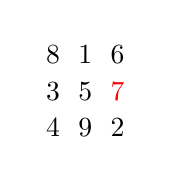
\begin{tikzpicture}
        \matrix[matrix of nodes]
        {
          8 & 1 &         6 \\
          3 & 5 & |[red]| 7 \\
          4 & 9 &         2 \\
        };
      \end{tikzpicture}
    %\includegraphics[width=0.35\textwidth]{figs/c-16.png}
    \caption{若尔当定理} 
    \label{fig:nrddl}
\end{figure}

\begin{theorem}[若尔当定理]\label{} \index{}
	任意一条简单闭曲线$C$把复平面$z$唯一地分成三个互不相交的点集 :
	\begin{inparaenum}[(i)]
	  \item $C$, 所有$C$上的点。
	  \item $I(C)$, 所有$C$内部的点。
	  \item $E(C)$, 所有$C$外部的点。
	\end{inparaenum}
    其中 $I(C)$ 是一个有界区域, $E(C)$ 是一个无界区域。若简单折线$P$的一个端点
	属于$I(C)$ , 另一个端点属于$E(C)$, 则$P$ 必与$C$ 有交点. 如图[\ref{fig:nrddl}]所示。
\end{theorem}
说明:图[\ref{fig:nrddl}]中,
\begin{compactitem}
    \item 点集$C$是曲线,不是区域。
    \item 点集$C$是区域$I(C)$的边界,也是区域$E(C)$的边界。
\end{compactitem}

\begin{definition}\label{}\index{}
	对于区域 $D$,如果由属于$D$的点构成的任意一条简单闭曲线 $C$,都有$I(C)\subset D $,则称$D$为\emph{单连通区域},否则为\emph{多连通区域}。如图[\ref{fig:ntqu}]所示。
    \begin{figure}[h]
        \centering
        \includegraphics[width=0.75\textwidth]{figs/c-17.png}
        \caption{(a) 多连通区域,(b) 单连通区域}
        \label{fig:ntqu}
    \end{figure}
\end{definition}
说明:\begin{compactitem}
    \item 单连通区域是没有所谓的“洞”结构的区域,
    \item 是否存在在拓扑学中非常重要。
\end{compactitem}

\begin{definition}\label{}
	设闭集C是所含不止一个点的点集, 如果不能划分为两个无公共点的非空闭集,则称C为\emph{连续点集}。 若区域D的边界$\partial D$是一个或二个、三个、$\dots$、n个互不相交的连续点集构成,则称D为单连通区域或\emph{二连通、三连通、$\dots$、n连通区域}。
\end{definition}
说明:\begin{compactitem}
    \item 图[\ref{fig:ntqu} (a)]的边界含三个互不相交的连续点集,因此是三连通区域
    \item 洞的数目在拓扑学中也非常重要。
\end{compactitem}

\begin{example}
    指明下列不等式所确定的区域, 是有界的还是无界的,单连通的还是多连通的
    \[ \begin{aligned}
        & (1) Re(z^2) < 1, \qquad (2) |\arg z| < \pi/3, \qquad (3) |1/z| < 3 \\
        & (4) |z+1| +|z-1| <4, \qquad (5) |z-1|\cdot|z+1|<1 , \qquad (6) |z+ 1 +i| <1
    \end{aligned}\]
\end{example}
\emph{解:} (1) 取 $z=x+yi$
\[ \begin{aligned}
    Re(z^2) &= x^2 -y^2 \\
    Re(z^2) < 1 & \quad \Leftrightarrow  \quad  x^2 -y^2 < 1
\end{aligned}\]
这是双曲函数之间的部分, 因此是无界单连通区域。\\
(2) 取 $z=re^{i \theta}$
\[ \begin{aligned}
    |\arg z| < \pi/3 & \quad \Leftrightarrow  \quad  -\pi/3  <\theta < \pi/3 
\end{aligned}\]
这是一个角形域,也是一个无界单连通区域。\\
(3)变形
\[ \begin{aligned}
    |1/z| < 3  & \quad \Leftrightarrow  \quad  |z| > 3 
\end{aligned}\]
这是一个以原点为圆心半径为$\dfrac{1}{3}$的圆的外部区域,是一个无界二连通区域。\\
(4) $|z+1| +|z-1| <4$ \\
这是复平面到两定点的距离和为4的椭圆的内部区域, 因此是有界单连通区域。 \\
\begin{figure}[htbp]
    \centering
    \includegraphics[width=0.4\textwidth]{figs/cn5.png}
    \caption{双叶玫瑰线}
    %\label{fig:}
\end{figure}
(5) $|z-1|\cdot|z+1|<1$\\
取三角式,先计算边界 
\[ \begin{aligned}
    |z-1|\cdot|z+1| &=1 \\
    |r \cos \theta -1 + r i \sin \theta|\cdot|r \cos \theta +1 + r i \sin \theta| &=1 \\
    [(r \cos \theta -1)^2  + (r \sin \theta)^2 ] \cdot [(r \cos \theta +1)^2  + (r \sin \theta)^2 ] &=1 \\
    (r^2 +1)^2 -4(r \cos \theta)^2 &= 1 
\end{aligned}\]
得两个解: (i) $r=0$; (i) $r^2=2 \cos 2 \theta$, 这是双叶玫瑰线。 
\[|z-1|\cdot|z+1| <1 \]
是内部区域,注意到$r=0$连通左右,是有界单连通区域。\\
(6) $ 0<|z+ 1 +i| <1$ \\
是以($-1,-i$)点为圆心半径为$1$的圆的内部去心区域,是有界二连通区域。


\section{复变函数} 
复变函数是以复数为自变量的函数,是十九世纪数学研究的热点。它可以看作是高数中实变函数向复数域的扩充。因此,它的部分内容,如函数可导和解析的判定、函数积分、幂级数的展开等,与高数相应部分内容是极为相似的。但也有部分内容与实变函数明显不同。学习和使用时,要特别注意这些不同的地方。

复变函数重点在于函数的可微性与可积性,这在处理许多物理与工程问题上,有着天然的优势。如关于瑕积分的计算,就有着化繁为简的奇效。

\subsection{复变函数的定义}

\begin{definition}\label{}\index{}
	设$E$为一复数集, 如果存在某种对应关系$f$, 按照这种对应关系,对于$E$中的每一复变数$z= x+yi$, 都存在复变数$w = u+vi $与之对应,则称复变数$w$是复变数$z$的函数,简称\emph{复变函数}, 并记作 $$w = f (z ), \quad (z \in E)$$ 
	若对每个$z$都只存在惟一的复变数$w$与之对应, 则称 $f (z )$是\emph{单值复变函数};若存在两个或两个以上的 $w$与一个$z$对应的情况, 则称 $f (z )$是\emph{多值复变函数}。称$E$为函数$f ( z )$的\emph{定义域}, 并称$w$的所有值构成的集合$F$为函数$f ( z )$的\emph{值域},记为
    \[F: \left\{ w \mid w=f(z), z \in E \right\} \]
\end{definition}
说明:\begin{compactitem}
    \item 只要$E$中有一个$z$存在两个或两个以上的$w$与之对应的情况, $f (z )$就是多值复变函数。
    \item 单值函数要求每一个$z$只有惟一一个$w$与之对应,并没有要求$w$也只有惟一一个$z$与之对应。因此对于单值函数,存在$|F| \ge |E| $。
    \item 复自变量$z$和复因变量$w$之间的关系 $w = f (z )$可用两个二元实变函数
    \[ u =u(x,y), \quad  v =v(x,y)\]
    进行描述。
\end{compactitem}
比如,设$ w = f(z)$取如下具体形式 
\[ w = z^2 +2\]
若$z$采用三角表示,$w$采用代数表示,则有
   \[ \begin{aligned}
	 u+vi &=  r^2 (\cos \theta +i\sin \theta )^2 +2 \\ 
	 &= (r^2 \cos 2 \theta +2) + i r^2 \sin 2 \theta 
   \end{aligned}\] 
根据复数相等条件, 有
   \[ \begin{cases}
	 u = u(r,\theta) = r^2 \cos 2 \theta +2\\
	 v = v(r,\theta) =  r^2 \sin 2 \theta
 \end{cases}\]
 复变函数$w = f (z )$体现的是$(r, \theta)$与($u,v$)之间的对应关系。\\

 若两者都采用有序数对表示,则有
\[ \begin{aligned}
  (u,v)&= (x,y)^2 +(2,0) \\ 
  (u,v)&= (x^2 -y^2 +2,2xy)
\end{aligned}\] 
当然,可以写成
\[ \begin{cases}
  u = x^2 -y^2 +2\\
  v = 2xy
\end{cases}\]
复变函数$w = f (z )$体现的是有序自变量对($x,y$)与有序因变量对($u,v$)之间的关系, 它们构成四维空间 $( u , v , x , y )$ , 因此它们的关系难以在二维空间进行几何表示。如果把有序数对($x,y$)看成$z$-平面的点,有序数对($u,v$)看成$w$-平面的点, 则变成了点与点之间的对应。复变函数$w = f (z )$可看成$z$-平面的点集$E$与$w$-平面的点集$F$之间的关系。如图[\ref{fig:twopoint}]所示。
\begin{figure}[ht]
	\centering
	  \includegraphics[width=0.75\textwidth]{figs/c-18.png}
      \caption{复变函数描述两平面点集间的对应关系}
      \label{fig:twopoint}
\end{figure}
很明显,两点集的元素间有如下关系:
\begin{compactitem}
    \item 对于点集$E$中的每一点$z$, 相应的点$w = f ( z )$必是点集$F$
    中的一个点,
    \item 对于点集$F$中的每一点$w$, 在点集$E$中至少有一点$z$与之对应。
 \end{compactitem}

\begin{definition}\label{}\index{}
	如果用$z$-平面的点$z$表示自变量$z$的值, 而用$w$-平面的点$w$表示因变量$w$的值,那么复变函数$w = f(z)$在几何上可以看作从$z$-平面点集$E$到$w$-平面点集$F$的\emph{变换}。通常称为由函数$w = f(z)$构成的\emph{映射},并称$w$是$z$的\emph{像点},$z$是$w$的\emph{原像}。 
\end{definition}
\begin{figure}[htbp]
	\centering
	\includegraphics[width=0.7\textwidth]{figs/c-19.png}
	\caption{$\Delta ABC $与$\Delta A'B'C' $的映射关系}
	\label{fig:twotri}
  \end{figure}
  图[\ref{fig:twotri}]描述了,$z$平面$\Delta ABC $,通过函数$w = z^* $映射到了$w$平面$\Delta A'B'C' $的情况。原来四维的复杂的对应关系就这样轻松地用二维映射进行了图形化、形象化地描述。

\begin{example}
    把平面$\Delta ABC $绕点$(-2,1)$逆时针旋转45度, 得$\Delta A'B'C' $,如图[\ref{fig:twotri2}]所示。试写出它们之间的变换关系式。
\end{example}
\emph{解:}~$\Delta ABC$ 构成$z$平面点集$E$,$\Delta A'B'C'$ 构成$w$平面点集$F$,令$z_0 = (-2,1)$, 则有
\[ \begin{aligned}
    w-z_0 &= e^{i\pi /4}(z-z_0) \\
    w &=  (z-z_0)e^{i\pi /4} + z_0
\end{aligned} \]  
这正是两者之间的变换关系式。
\begin{figure}[htbp]
    \centering
    \includegraphics[width=0.6\textwidth]{figs/c-20.png}
    \caption{三角形的旋转变换}
    \label{fig:twotri2}
   \end{figure}

若绕点$(-2,1)$逆时针旋转45度并放大10倍,则有
\[ \begin{aligned}
    w-z_0 &= 10 e^{i\pi /4}(z-z_0) \\
    w &=  10 (z-z_0)e^{i\pi /4} + z_0
\end{aligned} \]    

\begin{example}
    在$z$平面有(1)双曲线$x^2 - y^2 =4$ 、(2)直线 $ y= \sqrt{3} x $ (3)圆弧 $\{(x,y) \mid x^2 + y^2 =4, x \ge 0, y \ge 0 \}$, 如图[\ref{fig:threetran}]所示。
	若通过函数$w= z^2 $进行映射,求它们在$w$平面的图像。
    \begin{figure}[htbp]
     \centering
     \includegraphics[width=0.8\textwidth]{figs/c-22.png}
     \caption{(a) z平面曲线, (b) w平面曲线}
     \label{fig:threetran}
    \end{figure}
\end{example}
\emph{解:} (1)由对应关系
\[ \begin{aligned}
    w &=z^2 \\ 
    u+v i &= (x^2 -y^2) + 2 xy i 
\end{aligned}\]
得 $$u = x^2 -y^2 =4$$
因此双曲线$x^2 -y^2 =4$在$w$平面对应直线$u=4$。\\
(2) 直线 $ y= \sqrt{3} x $的辐角为 $\theta _1 = \dfrac{1}{3} \pi, \theta _2 = \dfrac{1}{3} \pi + \pi $,
对应关系 $w =z^2 $要求辐角变成原来的二倍,即
$$\varphi _1  =  2 \theta _1 = \frac{2}{3} \pi \qquad \varphi _2 = 2 \theta _2 = \frac{2}{3} \pi + 2\pi = \varphi _1 $$
因此直线 $ y= \sqrt{3} x $在$w$平面对应一条射线 \\
(3) 圆弧 $\{(x,y) \mid x^2 + y^2 =4, x \ge 0, y \ge 0 \}$ 的复数表示
\[ z= 2 e^{i \theta}, \quad  (0 \le \theta \le \frac{\pi}{2}) \]
由对应关系
\[ \begin{aligned}
    w &=z^2 \\ 
    &= 4 e^{i 2 \theta} \\
    &= R e^{i \varphi}, \quad ( R=4, 0 \le  \varphi \le \pi)
\end{aligned}\]
因此此圆弧在$w$平面对应半圆。\\

\begin{example}
    试问函数$w = \dfrac{1}{z+1}$把z平面的下列曲线变换成了w平面的什么图形?
    \[ (1) x^2 + y^2 =1, \quad (2) y=x+1\]
\end{example}
\emph{解:} (1) 把公式 
\[ x= \frac{1}{2}(z + z^*), \qquad  y= \frac{1}{2i}(z - z^*) \]
代入,$x^2 + y^2 = 1$  有
\[ \frac{1}{4}(z + z^*)^2 - \frac{1}{4}(z - z^*)^2 =1\]
得$zz^* =1$\\
由变换关系 $w = \dfrac{1}{z+1}$, 得
\[ z=  \dfrac{1}{w} -1\]
代入上式
\[ \begin{aligned}
    (\dfrac{1}{w} -1)(\dfrac{1}{w^*} -1) &= 1
\end{aligned} \]
解得$w + w^* =1$, 因此有 
\[ u= \dfrac{1}{2}\]
即:z平面的圆$ x^2 + y^2 =1$被变换成了w平面的直线$u= \dfrac{1}{2}$ \\
(2) 把公式代入$y=x+1$,得
\[ \frac{1}{2i}(z - z^*) = \frac{1}{2}(z + z^*) +1 \]
把 $z=  \dfrac{1}{w} -1$ 代入上式,
\[ \frac{1}{2i} \left( \frac{1}{w} -  \frac{1}{w^*} \right)  =  \frac{1}{2} \left( \frac{1}{w} + \frac{1}{w^*} -2\right) +1 \]
两边同乘$2iw^* w^*$, 得
\[ w^* - w = i(w + w^*)\]
由 $ w -u = iv, \quad  w^*-u = - iv $, 可得
\[ w^* - w = -2 i v, \quad w^* + w = 2 u\]
代回,得 
\[ u = -v \]
即:z平面的直线$y=x+1$被变换成了w平面的直线$u= -v $ \\

\begin{example}
    在$z$平面有点集$\{ z \mid z = x+yi, \, x \in \mathbb{Z}, y \in \mathbb{Z}, \left\vert x \right\vert \le 3, \left\vert y \right\vert \le 3) \}$ 
    若通过函数 $w= e^z $ 进行映射,求它们在$w$平面的图像。
    \begin{figure}[htbp]
        \centering
        \includegraphics[width=0.8\textwidth]{figs/c-24.png}
        \caption{(a) z平面点集,(b) w平面点集}
        \label{fig:twoplantdots}
       \end{figure}
\end{example}
\emph{解:} (1)由对应关系 
\[ w= e^z = e^xe^{iy} =Re^{i\theta}\]
得模长
\[ R= e^3, e^2, e^1, e^0, e^{-1}, e^{-2}, e^{-3}\]
辐角
\[ \theta = -3, -2, -1, 0, 1, 2, 3\]
实现的是49点构成的点集从直角坐标系到极坐标系的变换,如图[\ref{fig:twoplantdots}]所示。\\

\begin{definition}\label{}\index{}
	设函数$w = f(z)$ 的定义集为$z$-平面的点集$E$, 函数值集为$w$-平面的点集$F$,那么$F$中的每个点必将与$E$中的一个或多个点对应。 因此在点集$F$也可确定一个函数$z= \varphi(w)$, 它是函数$w = f(z)$的\emph{反函数},也称映射$w = f(z)$的\emph{逆映射}。记为$z= f^{-1}(w)$。 逆映射是从$w$平面点集$F$到$z$平面点位集$E$之间的变换。
\end{definition}
说明:\begin{compactitem}
    \item 必存在 $\forall w \in F, w = f[\varphi(w)]$,
    \item 当反函数是单值函数时, 必存在 $\forall z \in E, z = \varphi [f(w)]$,
    \item 当函数与反函数都是单值时,则集合$E$和$F$之间构成一一映射。
\end{compactitem} 
~\\

\subsection{复变函数的极限}~\\

\begin{definition}\label{}\index{}
    设函数$w = f(z)$定义在$z_0$的去心领域$0<\left\vert z - z_0\right\vert < \rho $内,如果存在确定的数$w_0$, 对于任意给定的$\varepsilon >0 $, 相应地必有一个实数$\delta $,使得只要
    \[ 0<\left\vert z - z_0\right\vert < \delta, ( 0< \delta \le \rho )  \]
    都有 $\left\vert f(z) -w_0\right\vert < \varepsilon , $ 则称 $w_0$为函数 $f(z)$ 当 $z $趋于$z_0$ 时的\emph{极限},记为:
    \[ \lim_{z \to z_0} f(z) = w_0\] 
\end{definition}
说明:\begin{compactitem}
    \item 若极限 $\lim\limits_{z \to z_0} f(z) = w_0$
	存在,则必然唯一,与$z \to z_0$ 的具体路径无关。
    \item 当$z$-平面的变点$z$进入一个充分小的$z_0$的$\delta $-去心邻域时, 它在$w$-平面的像点就落入$w_0$ 的一个任意给定的 $\varepsilon$-邻域内。如图[\ref{fig:qxry}]所示。
    \begin{figure}[htbp]
      \centering
      \includegraphics[width=0.7\textwidth]{figs/c-23.png}
      \caption{趋于方式的任意性示意图}
      \label{fig:qxry}
    \end{figure} 
    \item 极限的存在是研究复变函数一切重要性质的前提。
\end{compactitem}

\begin{theorem}\label{} \index{}
    设$f(z) = u(x,y) + i v(x,y), z_0 = x_0 + i y_0, w_0 = u_0 + i v_0$,那么存在极限$ \lim\limits_{z \to z_0} f(z) = w_0 $ 的充要条件为:两实变函数$u(x, y), v(x,y)$ 在点($x_0, y_0$)处存在极限
    \[ \lim _{\substack{x \rightarrow x_{0} \\ y \rightarrow y_{0}}} u(x, y)=u_{0}, \quad \lim _{\substack{x \rightarrow x_{0} \\ y \rightarrow y_{0}}} v(x, y)=v_{0}\]
\end{theorem}
说明:\begin{compactitem}
    \item 该定理把复变函数的极限问题转化为两个二元实变函数的极限问题。
    \item 二元实变函数的极限具有惟一性,与$x \rightarrow x_{0} $ 及$y \rightarrow y_{0} $ 的具体路径无关。
\end{compactitem}

\begin{proof}
  (1) 必要性:如果存在$ \lim\limits_{z \to z_0} f(z) = w_0 $ ,根据定义,当$z$进入$\delta$-领域时 
  $$0<\left\vert (x+iy) - (x_0+iy_0)\right\vert < \delta$$
  则$w$必进入$\varepsilon$-领域
  $$\left\vert (u+iv) - (u_0+iv_0)\right\vert < \varepsilon$$
  也就是说
  $$\left\vert (u-u_0) + i(v-v_0)\right\vert < \varepsilon$$
  可得 
  $$\left\vert u-u_0\right\vert < \varepsilon,\quad \left\vert v-v_0\right\vert < \varepsilon$$
  根据实变函数极限的定义,即存在 
  \[ \lim _{\substack{x \rightarrow x_{0} \\ y \rightarrow y_{0}}} u(x, y)=u_{0}, \quad \lim _{\substack{x \rightarrow x_{0} \\ y \rightarrow y_{0}}} v(x, y)=v_{0}\]
  (2)充分性:若
  \[ \lim _{\substack{x \rightarrow x_{0} \\ y \rightarrow y_{0}}} u(x, y)=u_{0}, 
  \quad \lim _{\substack{x \rightarrow x_{0} \\ y \rightarrow y_{0}}} v(x, y)=v_{0}\]
  则必有$$ \left\vert u - u_0 \right\vert  < \dfrac{\varepsilon}{2},\qquad  \left\vert v - v_0 \right\vert  < \dfrac{\varepsilon}{2} $$
  因此 
  $$ \left\vert u - u_0 \right\vert  + \left\vert v - v_0 \right\vert  <  \varepsilon $$
  那么,根据三角不等式,有 
  \[ \left\vert w -  w_0   \right\vert  \le \left\vert u - u_0 \right\vert  +  \left\vert v - v_0 \right\vert < \varepsilon\]
  说明当 $0<\left\vert z- z_0 \right\vert < \delta$时,$w$进行了任意小的$\varepsilon$-领域, 也即
  \[ \lim\limits_{z \to z_0} f(z) = w_0 \]
\end{proof}

\begin{theorem}\label{} \index{}
    若定义于点集$E$的两函数 $f(z), g(z)$ 在 $z_0$ 存在极限
	  \[\lim_{z \to z_0} f(z) = w_{1}, \, \lim_{z \to z_0} g(z) = w_{2}, \]
	  则它们的各、差、积、商也存在极限
	  \[ \begin{aligned}
		 \lim\limits_{z \to z_0} [f(z) \pm g(z)] &= w_{1} \pm w_{2} \\
		 \lim\limits_{z \to z_0} [f(z)g(z)] &= w_{1}w_{2} \\
			\lim\limits_{z \to z_0} [f(z)/g(z)] &= w_{1}/w_{2} 
	  \end{aligned}\]
\end{theorem}
说明:\begin{compactitem}
    \item 复变函数极限四则运算法则与实变函数的类似。
\end{compactitem}
\begin{example}
    试证明, 当$z\to 0$时,函数 $f(z) = \dfrac{Re(z)}{\left\vert z\right\vert}$的极限不存在
\end{example}
\begin{proof}
    (1) 令$z = x + y i, w = u + v i$, 有 
    \[f(z) = \frac{x}{\sqrt{x^2 + y^2}} \]
    因此 
    \[ u(x,y) = \frac{x}{\sqrt{x^2 + y^2}}, \, v(x,y) =0\]
    当$z$沿直线 $y= k x $ 趋于零时,有 
    \[ \begin{aligned}
     \lim _{\substack{x \rightarrow 0 \\ y \rightarrow 0}} u(x, y) &=\lim _{\substack{x \rightarrow 0 \\ y =  k x}}  \frac{x}{\sqrt{x^2 + y^2}} \\
     &= \lim_{x \to 0} \frac{x}{\sqrt{x^2 + k^2x^2}} \\
     &= \lim_{x \to 0} \frac{x}{ \left\vert x\right\vert\sqrt{1+ k^2}} \\
     &= \pm \frac{1}{\sqrt{(1+ k^2)}} 
    \end{aligned}\]
    值不唯一,因此, 当$z\to 0$时,  
    $$f(z) = \frac{Re(z)}{\left\vert z\right\vert}$$的极限不存在 \\
    (2) 采用三角表示,则
    \[ f(z) = \frac{r \cos \theta }{r} = \cos \theta \]
    若$z$沿实轴正方向趋0, 则 $\arg z = \theta =0$, $f(z) \to 1$, 
    若$z$沿y轴正方向趋0, 则 $\arg z = \theta =\pi/2$, $f(z) \to 0$,
    值不唯一,因此, 当$z\to 0$时, 
    $$f(z) = \frac{Re(z)}{\left\vert z\right\vert}$$的极限不存在。
\end{proof}

\subsection{复变函数的连续性}~\\

\begin{definition}
    \label{}\index{}
    设函数$w = f(z)$定义在点集$E$上,如果存
    在极限\[ \lim_{z \to z_0} f(z) = f(z_0), z \in E\] 
    则称函数$f(z)$在$z_0$点连续。对于曲线$C$,如果存
    在极限\[ \lim_{z \to z_0} f(z) = f(z_0), z \in C\]
    则称函数$f(z)$在曲线$C$上$z_0$处连续。如果函数$f(z)$在$C$内处处连续, 则称函数$f(z)$在曲线$C$上连续。如果$f(z)$在区域$D$ 内处处连续,则称函数$f(z)$在区域$D$连续。
\end{definition}

\begin{theorem}\label{} \index{}
设$f(z) = u(x,y) + i v(x,y), z_0 = x_0 + i y_0, w_0 = u_0 + i v_0 $,那么$ f(z) $ 在 $z_0$ 连续的充要条件是 :实变函数 $u(x,y)$和$v(x,y) $在点($x_0, y_0$)处连续,
  \[ \lim _{\substack{x \rightarrow x_{0} \\ y \rightarrow y_{0}}} u(x, y)=u(x_0, y_0), \quad \lim _{\substack{x \rightarrow x_{0} \\ y \rightarrow y_{0}}} v(x, y)=v(x_0, y_0)\]
\end{theorem}
说明:\begin{compactitem}
    \item 该定理把复变函数的连续性问题转化为两个二元实变函数的连续性问题。
\end{compactitem}
对于复变函数$$f(z) = \ln (x^2 + y^2) + i (x^2 -y^2)$$
由于实函数$u(x,y) = \ln (x^2 + y^2) $ 在除原点外的x-y平面处处连续,
而实函数$v(x,y) = x^2 -y^2 $ 在x-y平面处处连续,
因此复变函数$f(z)$在除原点外的复平面处处连续。

\begin{theorem}\label{} \index{}
 若 $f(z), g(z)$ 在 $z_0$ 连续, 则它们的各、差、积、商(分母不为零)也在 $z_0$ 连续。
\end{theorem}

\begin{theorem}\label{} \index{}
若函数$h = g(z)$在 $z_0$ 连续,  函数$w = f(z)$在 $h_0 = g(z_0)$ 连续, 那么复合函数 
        \[ w = f[g(z)]\]
        在 $z_0$连续。  
\end{theorem}
比如:\\
(1) 多项式函数  
\[ w = P(z) = a_0 + a_1 z + a_2 z^2 + \cdots + a_n z^n\]
在复平面内处处连续. \\
(2) 多项式有理分式函数
\[ w = \frac{ P(z) }{ Q(z) } \]
在复平面内使分母多项式不为零的点处处连续.

\begin{example}
    试证明函数
    \[ f(z) = \frac{1}{2i} \left(\frac{z}{z^*} - \frac{z^*}{z} \right)\]
    在原点处不连续
\end{example}
\begin{proof} 先化简
    \[ \begin{aligned}
      f(z) &= \frac{1}{2i} \left(\frac{z}{z^*} - \frac{z^*}{z} \right)\\
      &=  \frac{1}{2i}  \frac{z^2 - z^{*2} }{zz^* } \\
      &=  \frac{1}{2i}  \frac{(z- z^{*}) (z+z^{*})  }{zz^* } \\
    \end{aligned}\]   
    $z$取三角式,
    \[ \begin{aligned}
        f(z) = \frac{1}{2i r^2} (2r i \sin \theta) (2r \cos \theta) 
        &= \sin  2 \theta
      \end{aligned} \]  
      若$z$沿正实轴方向趋于原点,则有$\theta = 0$ 
      \[ \lim_{z \to 0} = \sin 0 = 0\]
      若$z$沿第一象限的平分线方向趋于原点,则有 $\theta = \frac{\pi}{4}$
      \[ \lim_{z \to 0} = \sin  2  \frac{\pi}{4} = 1\]
      不唯一,因此复变函数$f(z)$在原点处不存在极限, 因此不连续.  
\end{proof}

\begin{example}
    试证明:如果函数 $f(z) $ 在$z_0$连续,则 $g(z) = f^*(z)$也在$z_0$连续。
\end{example}
\begin{proof} 
    设 $$f(z) = u(x,y) + iv(x,y)$$则 $$g(z) =f^*(z) = u(x,y) - iv(x,y)$$ 
    
    如果$f(z) $ 在$z_0$连续, 则 $u(x,y)$ 和 $v(x,y)$ 都在$(x_0, y_0)$处连续。因此$u(x,y)$ 和 $-v(x,y)$ 也在$(x_0, y_0)$处连续。
    
    故$g(z)$在$z_0$处连续。
\end{proof}

\begin{Exercises}
    \item 试把 $z= \sqrt{-12} -2 i$ 化成指数形式
    \item 试证明 
    \begin{compactenum}[(1)]
        \item $\arg (z_1 z_2) = \arg z_1 + \arg z_2 + 2k_a \pi $,
        \item $\arg (\dfrac{z_1}{z_2}) = \arg z_1 - \arg z_2 + 2k_b \pi $,
    \end{compactenum}
    式中$k_a, k_b$ 各表示某个适当的整数。
    \item 试证明 $z_1,z_2, z_3$ 三点共线的充要条件为
    \[ \Im \frac{z_3 - z_1}{z_2 -z_1} = 0\]
    \item 试证明 
	\[ (e^{in\theta})^{\frac{1}{n}}  \ne e^{i \theta}, \quad n \in \mathbb{Z}^+\]
	\item 试证明
    \[ \left\vert z_1 + z_2\right\vert ^2  + \left\vert z_1 - z_2\right\vert ^2  = 2 \left( \left\vert z_1 \right\vert ^2 + \left\vert z_2 \right\vert ^2\right) \]
    并说明其几何意义
    \item 已知一正方形$z_1 z_2 z_3 z_4$的相对顶点的坐标
    \[ z_1 = (0,-1), z_3 = (2,5)\]
    求其他两个顶点的坐标
    \item 试计算 (1) $\sqrt[4]{1+i}$, (2) $ (1+i)^6$的值.
    \item 当$|z| \le 1$时,求$|z^n + z_0|$的最大值,其中n为正整数。
    \item 设$n \in \mathbb{Z}^+$, 若$(1+i)^n = (1-z)^n$,试求n的值
    \item 试将旋转公式
    \[ \begin{cases}
        x = x_1 \cos \theta -y_1 \sin \theta \\
        y = x_1 \sin \theta  + y_1 \cos \theta 
    \end{cases}
    \] 转化为复数形式
    \item 试证明 (1)复平面上的直线方程可写成
            \[ a z^* + a^* z = c, \quad (a \ne 0, a \in \mathbb{C}, c \in \mathbb{C})\]
            (2) 复平面上的圆周方程可写成
            \[ zz^* +a z^* + a^* z + c =0, \quad (a \in \mathbb{C}, c \in \mathbb{R})\]
    \item 试问不等式 \[0< \arg \frac{z-i}{z+i} < \frac{\pi}{4}\]
    确定的点集是不是一个区域,如果是则明确其类型。
    \item 试问函数$w = \dfrac{1}{z +1}$把z平面的下列曲线分别变换成了w平面的什么图形
    \[ (1)y=1, \quad (2) y=x, \quad (3) (x-1)^2 +y^2 -2 y =1 \]
    \item 求满足关系式$\cos \theta < r < 3 \cos \theta, \, (-\pi/2 < \theta < \pi /2 )$的点$z = r(\cos \theta + i \sin \theta)$的点集$D$, 然后判定$D$是不是区域,如果是它是单连通的还是多连通的?
    \item 试描出下列不等式所确定的区域或闭区域,并指明它们的有界的还是无界的,是单连通的还是多连通的
    \[(1) Im(z)> 0, \quad (2) |z-2| =4, \quad (3) 0< Re(z) <1, \quad (4) 2\le |z+1|\le 4\]
    \[(5) |z-1| < 4|z+1|, \quad (6) |z-2| + |z+2| \le 6, \quad (7) zz^* =(2+i) z -(2-i)z^* \le 4 \]
    \item 试证明函数 
    \[ f(z) = \frac{1}{2i} \left( \frac{z}{z^*} -\frac{z^*}{z} \right) \]
    当$z \to 0$时的极限不存在。
    \item 若函数$f(z)$在$z_0$处连续且$f(z_0) \ne 0$,试证明可以找到$z_0$的小领域,在这个领域内$f(z) \ne 0$.
    \item 试证明$f(z) = \arg z$ 在原点及负实轴上不连续。
    \item 试证明$f(z) = u(x,y) + i v(x,y)$ 在点$z_0 = x_0 + i y_0$处连续的充要条件为二🈚元函数$u(x,y)$ 和$v(x,y)$都在$(x_0, y_0)$点连续。
    \item 作图 
    \[ \begin{aligned}
        &(1)  |z-5|=6 ;\quad 
        (2)  |z+2 i| \geqslant 1 \\
        &(3)  \operatorname{Re}(z+2)=-1 ;\quad 
        (4)  \operatorname{Re}(\mathrm{i} \bar{z})=3 \\
        &(5)  |z+i|=|z-i| ;\quad 
        (6)  |z+3|+|z+1|=4 \\
        &(7)  \operatorname{Im}(z) \leqslant 2 ;\quad 
        (8)  \left|\frac{z-3}{z-2}\right| \geqslant 1 \\
        &(9)  0<\arg z<\pi ;\quad 
        (10)  \arg (z-i)=\frac{\pi}{4}  
    \end{aligned}\]
    \item 作出函数 $w = \dfrac{1}{z}$把下列z平面的曲线或区域变换成w平面的图形
    \[ \begin{aligned}
        &(1) (x-1)^2 +y^2 =4 ;\quad 
        (2)  y > x\\
        &(3)  x=-1 ;\quad 
        (4)   \arg z =\pi 
    \end{aligned}\]
\end{Exercises} 
 % 复数与复变函数
	%% To be included
\chapter{解析函数}
解析函数是一类具有特定性质的可微函数。本章首先引入判断函数可微或解析的主要条件:柯西-黎曼方程, 然后把实数域中常用的初等函数推广到复数域,并研究它们的性质。

\section{解析函数基本概念}\label{}

\subsection{复变函数的导数}

\begin{definition}
    \label{}\index{}
    设复变函数$w = f(z)$定义于区域$E$,$z_0$是$E$内一点,且$z_0 + \Delta z$依然在$E$内,
    如果存在极限
    \begin{equation}
        \lim_{\Delta z \to 0} \frac{\Delta w}{\Delta z}= \lim_{\Delta z \to 0}  \frac{f(z_0 +  \Delta z) - f(z_0)}{\Delta z}
    \end{equation}
   则称函数$f(z)$在$z_0$点可导。这个极限值称为函数$f(z)$在$z_0$点的\emph{导数},记为
    \begin{equation}
        f'(z_0) = \left.\frac{\mathrm{d} w }{\mathrm{d} z} \right|_{z=z_0} = \lim_{\Delta z \to 0} \frac{\Delta w}{\Delta z}= \lim_{\Delta z \to 0}  \frac{f(z_0 +  \Delta z) - f(z_0)}{\Delta z}
    \end{equation}
\end{definition}
考虑自变量发生变化$\Delta z$时, 因变量对应地发生变化$\Delta w$,令它们的比值为
\[ A = \frac{\Delta w}{\Delta z}\]
因此有 
\[ |\Delta w| = |A| |\Delta z|, \quad \text{Arg}(\Delta w) -\text{Arg}(\Delta z) = \text{Arg}(A)  \]
即:$|A|$是两个变化量之间的伸缩率,$\text{Arg}(A) $是两个变化量之间的夹角。如果函数$f(z)$在$z_0$点可导,则对于任意极小的变化量$\Delta z$, 比值$\dfrac{\Delta w}{\Delta z}$恒为$A$。这说明两个变化量之间的伸缩率和夹角都保持不变,称为\emph{保形性}。因此可导的几何意义就是函数在$z_0$附近具有保形性。如果不具有保形性,则不可导。实变函数的导数只描述伸缩率的不变性,复变函数的导数同时描述了伸缩率和夹角的不变性。

导数也可采用$\varepsilon-\delta$语言进行定义:
\begin{definition}
  \label{}\index{}
  设函数$w = f(z)$定义于区域$E$,$z_0$是$E$内一点,且$z_0 + \Delta z$依然在$E$内,
  对于任意给定的$\varepsilon>0$, 存在一个$\delta>0$, 使得当$|\Delta z|< \delta$时,有
  \[\left|\frac{f(z_0 +  \Delta z) - f(z_0) }{\Delta z} - f'(z_0)\right| < \varepsilon\] 
  成立,则称函数$f(z)$在$z_0$点可导,并称$f'(z_0)$是函数$f(z)$在$z_0$点导数。
\end{definition}
说明:\begin{compactitem}
    \item 函数在某点的导数具有惟一性,与$\Delta z \to 0$的具体路径无关。
    \item 若函数$f(z)$在$z_0$点可导,则函数$f(z)$在$z_0$点必然连续。
    \item 若函数$f(z)$在$z_0$点连续,则函数$f(z)$在$z_0$点不一定可导。
\end{compactitem}

\begin{example}
  由导数的定义求函数
\[ f(z) = z^2\]
的导数.
\end{example}
\emph{解:} 根据导数的定义,有 
\[ \begin{aligned}
f'(z) &= \lim_{\Delta z \to 0 }  \frac{f(z +  \Delta z) - f(z)}{\Delta z} \\
&= \lim_{\Delta z \to 0 }  \frac{(z +  \Delta z)^2 - z^2}{\Delta z} \\
&=  \lim_{\Delta z \to 0 } (2z +  \Delta z) \\
&= 2z
\end{aligned}\]

\begin{definition}
      \label{}\index{}
      如果函数$w =f(z)$在$z_0$点可导, 则
      \[ \Delta w = f(z_0 + \Delta z) - f(z_0) =  f'(z_0)\cdot \Delta z + O(\Delta z)\Delta z
      \]
      式中$\lim\limits_{\Delta z \to 0} O(\Delta z) =0 $,$ \left\vert O(\Delta z)\Delta z\right\vert$ 是 $\left\vert \Delta z \right\vert$的高阶无穷小,$f'(z_0)\cdot \Delta z$是函数$w = f(z)$ 对于改变量$\Delta w$的线性部分,称为函数$w = f(z)$ 在点 $z_0$的\emph{微分},记为
      \[ \mathrm{d}w = f'(z_0)\cdot \Delta z\]
      函数$w = f(z)$ 在点 $z_0$的微分存在,则称$w = f(z)$ 在点 $z_0$可微。如果$w = f(z)$ 在区域$E$处处可微,则称函数$w = f(z)$ 在区域$E$可微。 
  \end{definition}
  特别地,当$f(z) =z$时,有 $f'(z) =1$
  \[ \mathrm{d}w = \mathrm{d}z = f'(z)\Delta z = \Delta z \]
  因此有
  \[ \mathrm{d}w = f'(z_0)\cdot \Delta z = f'(z_0) \mathrm{d} z\]
  可得
  \[ f'(z_0) = \left.\frac{\mathrm{d} w }{\mathrm{d} z} \right|_{z=z_0} \]
  因此,函数在点 $z_0$可微与函数在点 $z_0$可导是等价的。
  
  \begin{theorem}\label{} \index{}
        函数$f(z) = u(x,y) + iv(x,y)$ 定义在区域$E$, 则函数$f(z)$ 在$E$内一点$z = x+y i$ 可微/可导的充要条件为:
        \begin{compactenum}[(i)]
          \item 实函数$u(x,y)$和$v(x,y)$在点$(x,y)$可微/可导  
          \item 实函数$u(x,y)$和$v(x,y)$在点$(x,y)$满足柯西-黎曼方程(C-R方程)
          \begin{equation}
            \frac{\partial u}{\partial x } = \frac{\partial v}{\partial y}, \quad \frac{\partial u}{\partial y } = - \frac{\partial v}{\partial x}
          \end{equation}
        \end{compactenum}
\end{theorem}
柯西-黎曼方程表明:可导的复变函数,其实部函数和虚部函数之间有联系,并不是相互独立的。柯西-黎曼方程可以简写成
\begin{equation}
  u_x= v_y, \quad u_y= - v_x
\end{equation}
\begin{proof}
  (1) 必要性, 设 
  \[ f(z) = u(x,y) + iv(x,y)\]
  有
  \[\frac{\Delta w}{\Delta z}=\frac{u\left(x_{0}+\Delta x, y_{0}+\Delta y\right)-u\left(x_{0}, y_{0}\right)}{\Delta x+i \Delta y}+i \frac{v\left(x_{0}+\Delta x, y_{0}+\Delta y\right)-v\left(x_{0}, y_{0}\right)}{\Delta x+i \Delta y}\]
  考虑 $f(z)$ 在点$z_0$处的导数,\\
  若从x方向逼近
  \[ \begin{aligned}
    f^{\prime}\left(z_{0}\right) &=\lim\limits _{\Delta x \rightarrow 0} \frac{u\left(x_{0}+\Delta x, y_{0}\right)-u\left(x_{0}, y_{0}\right)}{\Delta x}+i \lim\limits_{\Delta x \rightarrow 0} \frac{v\left(x_{0}+h, y_{0}\right)-v\left(x_{0}, y_{0}\right)}{\Delta x} \\
    &=\frac{\partial u}{\partial x}\left(x_{0}, y_{0}\right)+i \frac{\partial v}{\partial x}\left(x_{0}, y_{0}\right)
    \end{aligned}\] 
    若从y方向逼近
    \[ \begin{aligned}
      f^{\prime}\left(z_{0}\right) &=\lim\limits _{\Delta y \rightarrow 0} \frac{u\left(x_{0}, y_{0} +\Delta y\right)-u\left(x_{0}, y_{0}\right)}{i \Delta y}+i \lim\limits_{\Delta y \rightarrow 0} \frac{v\left(x_{0}, y_{0}+\Delta y\right)-v\left(x_{0}, y_{0}\right)}{i\Delta y} \\
      &=\frac{\partial v}{\partial y}\left(x_{0}, y_{0}\right)-i \frac{\partial u}{\partial y}\left(x_{0}, y_{0}\right)
      \end{aligned}\] 
    如果可导,则两条不同路径得到的结果必相等, 得柯西-黎曼方程 
    \[ \frac{\partial u}{\partial x } = \frac{\partial v}{\partial y}, \quad \frac{\partial u}{\partial y } = - \frac{\partial v}{\partial x}\]
    因此柯西-黎曼方程是必要条件,即:若函数$f(z)$在$z_0$不满足柯西-黎曼方程,则在$z_0$点不可微/不可导。\\
    (2) 充分性, 设 
    \[ h= h_1 + ih_2\]
    由两实函数的可微性 
    \[
    \begin{aligned}
    & u\left(z_0+h\right)-u\left(z_0\right)=\frac{\partial u}{\partial x}\left(z_0\right) h_1+\frac{\partial u}{\partial y}\left(z_0\right) h_2+o(h) \\
    & v\left(z_0+h\right)-v\left(z_0\right)=\frac{\partial v}{\partial x}\left(z_0\right) h_1+\frac{\partial v}{\partial y}\left(z_0\right) h_2+o(h)
    \end{aligned}
    \]
    由柯西-黎曼方程
    \[v\left(z_0+h\right)-v\left(z_0\right)=-\frac{\partial u}{\partial y}\left(z_0\right) h_1+\frac{\partial u}{\partial x}\left(z_0\right) h_2+o(h)\]
    所以,有
    \[\begin{aligned}
      u\left(z_0+h\right)+i v\left(z_0+h\right)-u\left(z_0\right)-i v\left(z_0\right) &=\left(\frac{\partial u}{\partial x}-i \frac{\partial u}{\partial y}\right)\left(h_1+i h_2\right) \\
      & =f^{\prime}\left(z_0\right)\left(h_1+i h_2\right)+o(h)
    \end{aligned}\]
    即复函数$f(z)$ 在点$z_0$处可导。
\end{proof}

\begin{example}
    试确定复变函数
  \[ f(z) = x + 2y i\]
  是否可导
\end{example}
\emph{解:} 函数若可导,要求存在极限
\[\lim_{\Delta z \to 0 }  \frac{f(z +  \Delta z) - f(z)}{\Delta z} \]
取$z= x+yi$代入,得
\[ \begin{aligned}
  \lim_{\Delta z \to 0 }  \frac{f(z +  \Delta z) - f(z)}{\Delta z}  &= \lim_{\Delta z \to 0 }  \frac{(x +  \Delta x)  + 2(y +  \Delta y) i  - (x + 2y i )}{\Delta x + \Delta y i}  \\ 
  &= \lim_{\Delta z \to 0 } \frac{\Delta x + 2 \Delta y i} {\Delta x +  \Delta y i} 
\end{aligned}\]
(1) 若$z+ \Delta z$沿着与x轴平行的方向趋于$z$, 则有 $\Delta y =0$, 代入 
\[ \lim_{\Delta z \to 0 } \frac{\Delta x + 2 \Delta y i} {\Delta x +  \Delta y i}  =  \lim_{\Delta z \to 0 } \frac{\Delta x } {\Delta x }  =1 \]
(2) 若$z+ \Delta z$沿着与y轴平行的方向趋于$z$, 则有 $\Delta x =0$, 代入 
\[ \lim_{\Delta z \to 0 } \frac{\Delta x + 2 \Delta y i} {\Delta x +  \Delta y i}  =  \lim_{\Delta z \to 0 } \frac{2 \Delta y i } {\Delta y i }  =2 \]
不具唯一性,极限不存在,因此复变函数 $f(z) = x + 2y i$ 不可导。

\begin{example}
  试证明函数$f(z) = \sqrt{xy}$在$z=0$处不可导但满足C-R方程
\end{example}
\begin{proof}
  (1) 计算比值 
  \[ \frac{\Delta w  }{\Delta z } = \frac{f(z) -f(0) }{z -0 } =  \frac{\sqrt{xy}}{x+yi } \]
  选取趋近方式为$y=kx$,代入上式 
  \[ \frac{\Delta w  }{\Delta z } = \frac{\sqrt{k}}{1+ik } \]
  这是个随k变的值,因此 $\lim\limits_{z \to 0} \frac{f(z) -f(0) }{z -0 } $ 不存在\\
  即函数$f(z) = \sqrt{xy}$在$z=0$处不可导。\\ 
  (2) 由于$w=\sqrt{xy} = u +i v $, 因此有 
  \[ u(x,y) = \sqrt{xy}, \qquad v(x,y)=0\]
  求四个偏分
  \[u_x(0,0) = \lim\limits_{x \to 0} \frac{u(x,0) -u(0,0) }{x -0 } =0 = v_y(0,0) \]
  \[u_y(0,0) = \lim\limits_{y \to 0} \frac{u(0,y) -u(0,0) }{y -0 } =0 = -v_x(0,0) \]
  即函数$f(z) = \sqrt{xy}$在$z=0$处满足C-R方程。
\end{proof}

\begin{example}
    试证明复变函数
    \[ f(z) = z ^n, \, n \in \mathbb{Z}^+\]
    在z平面处处可导。
\end{example}
\begin{proof}
    计算极限
  \[ \begin{aligned}
    \lim_{\Delta z \to 0 }  \frac{f(z +  \Delta z) - f(z)}{\Delta z}  
    &=   \lim_{\Delta z \to 0 }  \frac{(z +  \Delta z)^n - z^n}{\Delta z}  \\
    &=    \lim_{\Delta z \to 0 } \left[n z^{n-1} + \frac{n(n-1)}{2}z^{n-2} \Delta z + \cdots + (\Delta z)^{n-1} \right] \\
    &= n z^{n-1} 
  \end{aligned}\]
  极限处处存在,因此函数在z平面处处可导。
\end{proof}

\begin{example}
  试证柯西-黎曼方程具有如下极坐标形式
\begin{equation}
  u_r = \frac{1}{r}v_\theta, \quad v_r = -\frac{1}{r} u_\theta
\end{equation}
\end{example}
\begin{proof}
存在坐标变换关系
\[ \begin{cases}
	x = r\cos\theta \\
	y = r \sin \theta \\ 
\end{cases}\]
  根据二元函数链式求导法则,有
  \[ \begin{aligned}
    u_r &= u_x x_r + u_y y_r \\
        &= u_x \cos \theta + u_y \sin \theta \\
    u_\theta & = u_x x_\theta + u_y y_\theta \\
        & = -u_x  r \sin \theta  + u_y r \cos \theta 
  \end{aligned}\]
  同理可得
  \[ \begin{aligned}
    v_r &= v_x x_r + v_y y_r \\
        &= v_x \cos \theta + v_y \sin \theta \\
    v_\theta & = v_x x_\theta + v_y y_\theta \\
        & = -v_x  r \sin \theta  + v_y r \cos \theta 
  \end{aligned}\]
  代入
  \[ u_x = v_y, \quad u_y =-v_x\]
  得
  \[ v_r = -u_y \cos \theta + u_x \sin \theta, \quad  v_\theta = u_y  r \sin \theta  + u_x r \cos \theta  \]
  比较$u_r$与$v_\theta$,$v_r$与$u_\theta$, 得
  \[ u_r = \frac{1}{r}v_\theta, \quad v_r = -\frac{1}{r} u_\theta\]
\end{proof}

\begin{definition}
  如果 $f(z)$在区域$E$内任意一点都可导,则称$f(z)$在区域$E$可导。函数$f(z)$ 在区域$E$内每一点$z$的函数会随着$z$的变化而变化,因此这些导数构成一个关于$z$的函数,称为函数$f(z)$在区域$E$内的\emph{导函数},也简称导数,记为$f'(z)$或$\dfrac{dw}{dz}$。
  \end{definition}
  由二元函数求导公式并结合柯西-黎曼方程,得导数公式:
  \begin{equation}\label{} 
      \begin{aligned}
          f'(z) &= \frac{\partial u}{\partial x} + i \frac{\partial v }{\partial x} = \frac{\partial v}{\partial y} - i \frac{\partial u }{\partial y} = \frac{\partial u}{\partial x} - i \frac{\partial u }{\partial y} =
          \frac{\partial v}{\partial y} + i \frac{\partial v }{\partial x}   \\
      \end{aligned}
  \end{equation}
  因此,当$f(z)$可导时,仅由实部或者仅由虚部可以求出其导数。利用此公式求导,可免去分析极限所带来的困难。

~\\
\noindent\emph{导数的运算法则} 

复变函数的导数定义与实变函数的定义类似,因此复变函数的导数运算法则与实变函数的保持一致。
\begin{compactenum}[(1)]
  \item 导数的四则运算
  \begin{enumerate}
    \item $(c)' =0, \, c$为复常数 \vspace{0.3em}
    \item $(z^n)' =n z^{n-1}, \, n$为正整数 \vspace{0.3em}
    \item $ [f(z) \pm g(z)]' = f'(z) \pm g'(z)$ \vspace{0.3em}
    \item $ [f(z) g(z)]' = f'(z) g(z) + f(z) g'(z) $ \vspace{0.3em}
    \item $ \left[\dfrac{f(z)}{g(z)} \right]' = \dfrac{f'(z) g(z) - f(z) g'(z)}{g^2(z)}, \, \quad  g(z) \ne 0 $ 
  \end{enumerate}
  \item 复合函数的求导法则 $\left[ f(g(z))\right]' = f'(w)g'(z)$ 
  \item 反函数的求导法则  $ [f^{-1}]'(w)  = \left. \dfrac{1}{f'(z)} \right|_{z=f^{-1}(w)} = \dfrac{1}{f'[f^{-1}(w)]}  $
\end{compactenum}


\begin{example}
  求函数
    \[ f(z) = (3z^2 -4z +5)^{11}\]
  的导数.
\end{example}
\emph{解:} 由复合函数求导法则
\[ \begin{aligned}
  f'(z) &= 11 (3z^2 -4z +5)^{10} \cdot \frac{\mathrm{d}}{\mathrm{d}z } (3z^2 -4z +5) \\ 
  &=  11 (3z^2 -4z +5)^{10} (6z-4) \\
  &= 22(3z-2)(3z^2 -4z +5 )^{10}
\end{aligned}\]

\subsection{复变函数的解析性}

\begin{definition}\label{}\index{}
函数$w = f(z)$定义于区域$E$,$z_0$是$E$内一点,如果$f(z)$在$z_0$点及$z_0$的邻域内处处可导,则称$f(z)$在$z_0$点\emph{解析}。如果函数$f(z)$在$z_0$点不解析,则称$z_0$是函数$f(z)$的一个\emph{奇点}。\\
如果 $f(z)$在区域$E$内任意一点都解析,则称$f(z)$是区域$E$的一个\emph{解析函数},也称全纯函数或正则函数。
\end{definition}
说明:
\begin{compactitem}
    \item 解析函数这一重要概念, 是与相伴区域密切联系的。 函数$f(z)$在$z_0$解析,则函数$f(z)$在$z_0$可微。函数$f(z)$在$z_0$可微,但函数$f(z)$在$z_0$不一定解析, 因为它在其$z_0$的邻域内不一定处处可微。
    \item 函数$f(z)$在区域$E$可微/可导,则函数$f(z)$在区域$E$解析,两者是等价的。
    \item 通常泛称的解析函数是容许有奇点的, 但更主要的是, 它在复平面上总有解析点。
\end{compactitem}

\begin{example}
    分析下列函数的解析性
  \[ f(z) = z^2, \quad  g(z) = x+ 2yi, \quad h(z) =\left\vert z\right\vert^2 \]
\end{example}
  \emph{解:} (1)根据导数的定义,有 
  \[ \begin{aligned}
    f'(z) &= \lim_{\Delta z \to 0 }  \frac{f(z +  \Delta z) - f(z)}{\Delta z} \\
    &= \lim_{\Delta z \to 0 }  \frac{(z +  \Delta z)^2 - z^2}{\Delta z} \\
    &=  \lim_{\Delta z \to 0 } (2z +  \Delta z) \\
    &= 2z
  \end{aligned}\]
  即$f(z)$在复平面处处可导,根据解析函数的定义,它在整个复平面是解析函数.\\
  (2)根据导数的定义
  \[\lim_{\Delta z \to 0 }  \frac{g(z +  \Delta z) - g(z)}{\Delta z} \]
  取$z= x+yi$代入,得
  \[ \begin{aligned}
    \lim_{\Delta z \to 0 }  \frac{g(z +  \Delta z) - g(z)}{\Delta z}  &= \lim_{\Delta z \to 0 }  \frac{(x +  \Delta x)  + 2(y +  \Delta y) i  - (x + 2y i )}{\Delta x + \Delta y i}  \\ 
    &= \lim_{\Delta z \to 0 } \frac{\Delta x + 2 \Delta y i} {\Delta x +  \Delta y i} 
  \end{aligned}\]
  \begin{inparaenum}[(i)]
    \item 若$z+ \Delta z$沿着与x轴平行的方向趋于$z$, 则有 $\Delta y =0$, 代入 
    \[ \lim_{\Delta z \to 0 } \frac{\Delta x + 2 \Delta y i} {\Delta x +  \Delta y i}  =  \lim_{\Delta x \to 0 } \frac{\Delta x } {\Delta x }  =1 \]
    \item 若$z+ \Delta z$沿着与y轴平行的方向趋于$z$, 则有 $\Delta x =0$, 代入 
    \[ \lim_{\Delta z \to 0 } \frac{\Delta x + 2 \Delta y i} {\Delta x +  \Delta y i}  =  \lim_{\Delta y \to 0 } \frac{2 \Delta y i } {\Delta y i }  =2 \]
\end{inparaenum}
因此函数 $g(z) = x + 2y i$ 在复平面处处不可导,处处不解析。\\
(3)计算极限
  \[ \begin{aligned}
    \lim_{\Delta z \to 0 }  \frac{h(z_0 +  \Delta z) - h(z_0)}{\Delta z}  
    &=   \lim_{\Delta z \to 0 }  \frac{ \left\vert z_0 +  \Delta z \right\vert^2  - \left\vert z_0 \right\vert^2 }{\Delta z}  \\
    &=   \lim_{\Delta z \to 0 } \frac{(z_0 +  \Delta z) (z_0^* +  (\Delta z)^*) - z_0z_0 ^* }{\Delta z} \\
    &= \lim_{\Delta z \to 0 } \left( z_0^* + (\Delta z)^* + z_0\frac{(\Delta z)^*}{\Delta z}\right)
  \end{aligned}\]
  \begin{inparaenum}[(i)]
    \item 当$z_0=0$, 上式 $= 0$. 说明函数在原点可导。\\
    \item 当$z_0\ne 0$, 令 $\Delta z $沿直线 
    \[ y-y_0 = k(x-x_0)\]
    趋于$z_0$时,有
    \[ \begin{aligned}
      \frac{(\Delta z)^*}{\Delta z} &= \frac{\Delta x- i\Delta y }{\Delta x+ i\Delta y }  \\
      &= \frac{1- i \frac{\Delta y}{\Delta x} }{1+ i \frac{\Delta y}{\Delta x}} \\
      &=   \frac{1- ik }{1+ i k} 
    \end{aligned}\]
    由于$k$的任意性, 当$\Delta z$趋零时, $\dfrac{(\Delta z)^*}{\Delta z} $趋于的值不确定, 因此极限 $$\lim_{\Delta z \to 0 }  \dfrac{h(z_0 +  \Delta z) - h(z_0)}{\Delta z} $$ 不存在。
\end{inparaenum}
因此,函数$h(z) =\left\vert z\right\vert^2 $在复平面上处处不解析。

\begin{example}
    分析下列函数$f(z) =  z Re(z)$的解析性。
\end{example}
  \emph{解:} (1)取$z=0$
  \[ \begin{aligned}
    \lim_{\Delta z \to 0 }  \frac{f(z +  \Delta z) - f(z)}{\Delta z} 
    &= \lim_{\Delta z \to 0 }  \frac{f(0 +  \Delta z) - f(0)}{\Delta z}  \\
    &= \lim_{\Delta z \to 0 }  \frac{\Delta z Re (\Delta z)}{\Delta z} \\
    &= 0
  \end{aligned}\]
  即$f(z)$在原点可导。\\
  (2)取$z \ne 0$ 
  \[ \begin{aligned}
   \frac{f(z +  \Delta z) - f(z)}{\Delta z} 
   &=   \frac{(z +  \Delta z)  Re (z +  \Delta z) - z Re (z)}{\Delta z}  \\
   &= \frac{z}{\Delta z}[ Re (z +  \Delta z) - Re (z) ] +  Re (z +  \Delta z) \\
   &= \frac{z}{\Delta x + i \Delta y }[ x +  \Delta x - x ] +  (x + \Delta x) \\
   &= z \frac{\Delta x}{\Delta x + i \Delta y } + x + \Delta x 
 \end{aligned}\]
 计算两种趋近方案:\\ 
 \begin{inparaenum}[(i)]
    \item \[\begin{aligned}
    \lim _{\substack{\Delta  x = 0 \\ \Delta y \rightarrow 0}} \frac{f(z +  \Delta z) - f(z)}{\Delta z}   
     &=  \lim_{\Delta y \to 0 }  z \frac{0}{0+ i \Delta y } + x + 0 \\
     &= x 
 \end{aligned}\]
 \item \[\begin{aligned}
 \lim _{\substack{\Delta  y = 0 \\ \Delta x \rightarrow 0}} \frac{f(z +  \Delta z) - f(z)}{\Delta z}   
    &=  \lim_{\Delta x \to 0 }  z \frac{\Delta x }{\Delta x + i 0 } + x + \Delta x  \\
    &= z + x 
\end{aligned}\]
\end{inparaenum}
即$z \ne 0$的点,不可导,  \\
因此函数$f(z)$在复平面处处不解析。

\begin{theorem}\label{} \index{}
    对于两复数$f(z)$和$g(z)$, 在区域$E$内有定义, \\
    \begin{compactitem}
        \item 若 $f(z), g(z)$ 在区域$E$内解析, 
        则它们的各、差、积、商(分母不为零)在区域$E$也解析。
        \item 若函数$h = g(z)$在 区域$E$ 解析, 函数$w = f(z)$在$h$平面的区域$F$解析, 如果$E$内的每一个点$z$对应的函数值$ h=g(z)$都属于区域$F$, 则复合函数 
        \[ w = f[g(z)]\]
        在区域$E$ 解析。
    \end{compactitem}
\end{theorem}
特别地: \\
\begin{inparaenum}[(i)]
    \item 所有的多项式函数 $P(z)$在复平面处处解析。\\
    \item 有理分式函数$\dfrac{P(z)}{Q(z)}$在不含分母为零的点的区域解析,使分母为零的点是奇点。\\
\end{inparaenum}

\begin{theorem}\label{} \index{}
    函数$f(z) =u(x,y) +iv(x,y)$ 的定义域为$E$,
    \begin{compactitem}
    \item 它在定义域内解析的充要条件是:$u(x,y)$和$v(x,y)$ 在$E$内可微,并且满足柯西-黎曼方程 (C-R方程)
     \item  区域$D \subseteq E $,如果$u(x,y)$和$v(x,y)$的四个偏导函数$u'_x, u'_y, v'_x, v'_y$在$D$内存在、连续且满足柯西-黎曼方程 (C-R方程), 则函数$f(z)$在区域$D$内解析。 
    \end{compactitem}
\end{theorem}
~\\
函数解析的判定方法:
\begin{compactitem}
    \item 如果能用求导公式和法则证实复变函数$f(z)$的导数在区域$D$内处处存在,则可断定函数$f(z)$在区域$D$内解析。
    \item 如果函数$f(z) =u(x,y) +iv(x,y)$ 在区域$D$内有定义,$u(x,y)$和$v(x,y)$的四个偏导函数$u_x, u_y, v_x, v_y$都存在、连续且满足柯西-黎曼方程,则可断定函数$f(z)$在区域$D$内解析。
\end{compactitem}

\begin{example} \label{ex:gz}
试判定下列函数在何处可导,何处解析
  \[ f(z) = z^*, \, g(z) = e^x(\cos y + i \sin y), \,h(z) = z Re(z)\]    
\end{example}
\emph{解}
(1)由于 \[ u(x,y) + iv(x,y) = w = z^* = x -yi \]
    有 \[ u(x,y) =x, v(x,y) =-y\] 
计算四个偏微分  
     \[ \frac{\partial u}{\partial x} =1, \frac{\partial u}{\partial  y }=0, \frac{\partial v}{\partial x} =0, \frac{\partial v}{\partial y} =-1\]
     有$ \dfrac{\partial u}{\partial x} \ne \dfrac{\partial v}{\partial y} $,即不满足柯西-黎曼方程,故$f(z)$在复平面处处不可导,处处不解析。\\
(2) 由 $g(z) = e^x(\cos y + i \sin y)$, 可得 
     \[ u(x,y) =e^x\cos y, v(x,y) =e^x \sin y\] 
     计算四个偏微分 
     \[ \frac{\partial u}{\partial x} =e^x\cos y, \frac{\partial u}{\partial  y }=- e^x \sin  y, \frac{\partial v}{\partial x} =e^x \sin y, \frac{\partial v}{\partial y} =e^x \cos  y\]
     判定:\\
     \begin{inparaenum}[(i)]
       \item 四个一阶偏导数存在且连续\\
       \item $\dfrac{\partial u}{\partial x} = \dfrac{\partial v}{\partial y}, \, \dfrac{\partial u}{\partial  y } = -   \dfrac{\partial v}{\partial x}$
     \end{inparaenum}
因此 $g(z)$在复平面处处可导,处处解析。\\
根据导数公式,可求得  
    \[ \begin{aligned}
      g'(z) &= \frac{\partial u}{\partial x} + i \frac{\partial v }{\partial x} \\ 
      &= e^x\cos y +i e^x \sin y  \\
      &= g(z)
    \end{aligned}\]
(3) 由 $h(z) = z Re(z) = x^2 + i xy$ 可得
    \[ u(x,y) =x^2, v(x,y) =xy\] 
    计算四个偏微分 
    \[ \frac{\partial u}{\partial x} =2 x, \frac{\partial u}{\partial  y }=0, \frac{\partial v}{\partial x} =y, \frac{\partial v}{\partial y} =x\]
    判定:\\
    \begin{inparaenum}[(i)]
      \item 四个一阶偏导数存在且连续\\
      \item 当且仅当$x=y=0$时,满足柯西-黎曼方程
    \end{inparaenum}
因此 $h(z)$仅在原点可导,在复平面处处不解析。


 \begin{example}
    如果$f(z) =u(x,y ) + i v(x,y) $ 在区域$D$内是解析函数,且$f'(z) = 0, (z \in D) $, 试证明函数$f(z)$在区域$D$内是常函数。
 \end{example}
    \begin{proof}
    由导函数公式,有
    \[ f'(z) = u_x + i v_x = v_y - i u_y =0\]
    由复数相等条件
    \[ u_x = v_y = v_x = u_y =0\]
    因此有
    \[ u(x,y) = c_1, \qquad v(x,y) =c_2\]
    式中$c_1, c_2$为复常数,即
    \[ f(z) = u(x,y) + iv(x,y) = c_1 + i c_2 = C_1 + iC_2\]
    式中$C_1, C_2$为实常数。\\
    即:函数$f(z)$在区域$D$内是常函数。
    \end{proof}
 \begin{example}
    如果$f(z) =u(x,y ) + i v(x,y) $ 在区域$D$内是解析函数,且$f'(z) \ne 0 $, 试证明曲线族$u(x,y)=c_1$和$v(x,y) = c_2$ 必互相正交,其中$c_1, c_2$ 为常数。
 \end{example}
    \begin{proof}
        因为 $f'(z) = -\frac{1}{i}u_y + v_y \ne 0 $,所以 $v_y$和$u_y$不能全为零。\\
        (1)设曲线族$u(x,y)=c_1$和$v(x,y) = c_2$ 在某交点处$v_y$和$u_y$都不为零 \\
        根据隐函数求导法则,它们的斜率分别为:
         \[ k_1 = - \frac{u_x}{u_y}, \qquad k_2 = - \frac{v_x}{v_y}\]
        根据C-R方程,计算两者的积
        \[ k_1\cdot k_2 = \left(- \frac{u_x}{u_y}\right) \cdot \left(- \frac{v_x}{v_y}\right) = \left(- \frac{v_y}{u_y}\right) \cdot \left(- \frac{u_x}{v_y}\right) =-1\]
        因此两者正交。\\
        (2)如果交点处$v_y$和$u_y$有一个为零, 则另一个必不为零,那两曲线的切线一条水平,另一条垂直,它们依然相互正交。
    \end{proof}
\begin{example}
        如果$f(z) =u(x,y ) + i v(x,y) $ 在区域$D$内是解析函数,且$v= u^2 $, 求$f(z)$
\end{example}   
\emph{解:} 根据C-R方程,计算$u(x,y)$的偏导 
    \[\begin{aligned}
        u_x &= v_y = 2u u_y  \qquad (a)\\
        u_y &= -v_x = -2u u_x \qquad (b)
    \end{aligned}\]
    (1) 把(b)式代入(a)
    \[ u_x (4u^2 +1) =0\]
    由于$(4u^2 +1) \ne 0$, 得$u_x =0$ \\
    (2)若把(a)式代入(b),同理可得$u_y =0$ \\
    因此 
    \[ u'(x,y) = 0 \Rightarrow u(x,y)=c\]
    式中$c$为实常数。代回得 
    \[ f(z) =u(x,y ) + i v(x,y) = c+ ic^2 \]


\section{初等解析函数}\label{}
实数域的初等函数,比如三角函数,指数函数,对数函数,幂函数等,它们是一类性质各异且应用非常广泛的可微函数。本节我们将把这些常用的实数域初等函数推广到复数域,并分析它们的可微性、解析性等重要性质。\\

\subsection{指数函数}
~\\
在例[\ref{ex:gz}]中,我们看到函数
\[ f(z) = e^x (\cos y + i \sin y) \]
在复平面处处可微处处解析,且$f'(z) = f(z)$。这些性质与实数域中的指数函数$f(x) = e^x$完全相同。基此,可以定义复数域的指数函数。
\begin{definition}\index{}
	对于任意复数 $z= x +iy $, 由关系式
  \begin{equation}\label{eq:zshs}
    f(z) = e^z = e^{x+iy}  = e^x (\cos y + i \sin y) 
  \end{equation} 
规定的复函数$e^z$称为复数$z$的\emph{指数函数}, 通常记为 $\exp {z}$。
\end{definition}
在定义式[\ref{eq:zshs}]中,当$z$的实部$x=0$时,有 
\begin{equation}
  e^{iy}  = \cos y + i \sin y 
\end{equation} 
这正是欧拉公式,因此式[\ref{eq:zshs}]可以看成的实数域欧拉公式向复数域的推广。
可以看出,指数函数的模$|e^z| = e^x > 0$, 辐角$\arg (e^z) = y $, 实部$\text{Re}(e^z) = e^x \cos y$, 虚部$\text{Im}(e^z) = e^x \sin y$。

当$z$的虚部$y=0$时,复指数函数$f(z)= e^x$与实指数函数$f(x) = e^x$保持一致。同时,实指数函数的加法定理: $e^{x_1+x_2} = e^{x_1} e^{x_2}$ 在复指数函数中也得以保存,即有
\begin{equation}
  e^{z_1+z_2} = e^{z_1} e^{z_2},
\end{equation}
指数函数$e^z$具有如下主要性质:
\begin{compactenum}[(a)]
	\item 解析性:$e^z$在复平面$\mathbb{C}$解析,且$(e^z)' = e^z$,
	\item 加法定理:  $e^{z_1+z_2} = e^{z_1} e^{z_2}$,
	\item 周期性:$e^{z+2k\pi i } = e^{z}, \, (k=0, \pm 1, \pm 2, \dots)$,基本周期为$2\pi i$。
\end{compactenum}
说明:
\begin{compactenum}[(i)]
	\item $e^z= \exp {z}$只是一种记号, 不能理解为$(2.718\dots)^z$, 失去了幂的意义。
	\item 实指数函数$e^x$没有周期性。
\end{compactenum}

\begin{example}
  试证明函数$f(z) = e^{\bar{z}}$在复平面不解析
\end{example}
\begin{proof}
  由于$e^{\bar{z}} = e^x(\cos y - i \sin y)$, 有
  \[ u(x,y) = e^x \cos y, \qquad v(x,y) = - e^x \sin y \]
  求四个偏分
  \[ u_x = e^x \cos y,\, v_y = -  e^x \cos y\]
  只有在$k=k \pi + \pi /2 $时,才满足C-R方程 $u_x = v_y$, 因此$e^{\bar{z}}$在复平面不解析。 
\end{proof}

\begin{example}
  试求函数$f(z) = |e^{z^2}|$
\end{example}
\emph{解:} 令$z = x+ iy $, 有$z^2 = x^2 - y^2 + 2xyi$
\[ \begin{aligned}
  f(z) = |e^{z^2}| & = |e^{x^2 - y^2 + 2xyi}|  \\
  & = |e^{x^2 - y^2 } e^{2xyi}| \\
  & = e^{x^2 - y^2 } 
\end{aligned}\]

\begin{example}
  试求函数$e^{2+3i}$和$e^{2-3i}$的主辐角
\end{example}
\emph{解:} 因为$e^z = e^{x+ iy} = e^x(\cos y + i \sin y) $ 的辐角为
\[Arg (e^z) = y + 2k\pi, k \in \mathbb{Z} \]
代入,并根据辐角主值区间$\left(- \pi, \pi\right]$确定$k$的取值。 
\[Arg (e^{2+3i}) = 3 + 2k\pi, \qquad \arg (e^{2+3i}) = 3 \]
\[Arg (e^{2-3i}) = -3 + 2k\pi, \qquad \arg (e^{2-3i}) = -3 \]

\begin{example}
  试求函数$f(x) = e^{z/5}$的周期
\end{example}
\emph{解:} 由于$e^z$的周期为$2k\pi i$ 
\[ \begin{aligned}
  f(z) & =  e^{z/5} =  e^{z/5 + 2k\pi i}  \\
     & =  e^{\frac{z + 10k\pi i}{5}}  \\
     & = f(z+10k \pi i)
\end{aligned}\]
因此,函数$f(x) = e^{z/5}$的周期为$10k \pi i$。

\subsection{三角函数与双曲函数}
~\\
在公式
\[ e^{x+iy}  = e^x (\cos y + i \sin y) \]
中,取$x=0$, 得 
\[ e^{iy}  = \cos y + i \sin y \]
取复共轭,得
\[ e^{-iy}  = \cos y - i \sin y \]
两式相加减,得 
\begin{equation}\label{eq:ssjhs}
  \sin y =  \frac{e^{iy} - e^{-iy} }{2i}, \qquad \cos y =  \frac{e^{iy} + e^{-iy} }{2}
\end{equation}
这说明实数域的三角函数可以用表示成复函数形式。下面把它推广到复数域。
\begin{definition}
  对于任意复数 $z= x +iy $, 由关系式
  \begin{equation}\label{eq:fsjhs}
    \sin z =  \frac{e^{iz} - e^{-iz} }{2i}, \qquad \cos z =  \frac{e^{iz} + e^{-iz} }{2}
  \end{equation}
所规定的复函数$\sin z$和$\cos z$ 分别称为复数$z$的的\emph{正弦函数}和\emph{余弦函数}。
\end{definition}
在定义式[\ref{eq:fsjhs}]中,当$z$的虚部$y=0$时,正好是式[\ref{eq:ssjhs}]。即 复数域的三角函数与实数域的三角函数保持一致。\\
三角函数具有如下主要性质:
\begin{compactenum}[(a)]
	\item 解析性:$\sin z $和 $\cos z $在复平面$\mathbb{C}$解析,且
  \begin{equation}
   \sin' z = \cos z , \cos' z = -\sin z  
  \end{equation}
  \item 奇偶性:
  \begin{equation}
    \sin (-z) = - \sin z, \,\cos (-z) = \cos z
  \end{equation}
	\item 三角恒等式: 
  \begin{equation} 
    \begin{aligned}
      & \sin^2 z + \cos^2 z =1 \\
      & \sin(z_1 +z_2) = \sin z_1 \cos z_2 + \cos z_1 \sin z_2 \\
      & \cos(z_1 +z_2) = \cos z_1 \cos z_2 - \sin z_1 \sin z_2  \\
      & \sin 2 z = 2 \sin z \cos z \\
      & \tan 2 z = \frac{2 tan z}{1- tan ^2 z} \\
      & \sin \left( \frac{\pi}{2}- z\right) = \cos z, \quad \cos(z+ \pi) = - \cos z \\
      & |\cos z|^2 = \cos ^2 z + \sinh^2 y, \quad |\sin z|^2 = \sin ^2 z + \sinh^2
    \end{aligned}
  \end{equation}
	\item 周期性:
	\begin{equation}
    \sin(z+2\pi) = \sin z, \, \cos(z+2\pi) = \cos z
  \end{equation}
\end{compactenum}

\begin{proof}
  (1) 解析性 :  根据定义
  \[\sin z =  \frac{e^{iz} - e^{-iz} }{2i}, \qquad \cos z =  \frac{e^{iz} + e^{-iz} }{2}\]
  由于$e^{iz}$和$e^{-iz}$都在复平面$\mathbb{C}$解析,可得$\sin z$和$\cos z $也在复平面$\mathbb{C}$解析。\\ 
  (2)导数:
  \[ \begin{aligned}
    \sin z &=  \frac{e^{iz} - e^{-iz} }{2i} \\
    \sin' z &=  \frac{1}{2i} (e^{iz} - e^{-iz} )'\\
    &= \frac{1}{2} (e^{iz} + e^{-iz} ) \\
    & = \cos z
  \end{aligned}\]
  (3)周期性: 
  \[ \begin{aligned}
    \sin (z+2\pi) &=  \frac{e^{i(z+2\pi)} - e^{-i(z+2\pi)} }{2i} \\
    & =  \frac{e^{iz}e^{2\pi i}  - e^{-iz}e^{-2\pi i}  }{2i} \\
    &=  \frac{e^{iz} - e^{-iz} }{2i} \\
    & = \sin z
  \end{aligned}\]
  (4) 三角恒等式 \\
  \[ \begin{aligned}
    \sin^2 z & = -\frac{(e^{iz} - e^{-iz})(e^{iz} - e^{-iz}) }{4}  \\
    & = \frac{ - e^{i2z} - e^{-i2z} + 2 }{4} \\
  \end{aligned}\]
  \[ \begin{aligned}
    \cos^2 z & = \frac{(e^{iz} + e^{-iz})(e^{iz} + e^{-iz}) }{4}  \\
    & = \frac{ e^{i2z} + e^{-i2z} + 2 }{4} 
  \end{aligned}\]
  两式相加,得
  \[ \sin^2 z + \cos^2 z =1 \]
  和差化积 
  \[ \begin{aligned}
   \sin(z_1 + z_2) & =  \frac{e^{i(z_1+z_2)} - e^{-i(z_1+z_2)} }{2i} \\
   & =   \frac{e^{iz_1} e^{iz_2}  - e^{-iz_1} e^{-iz_2}}{2i} \\
   & =   \frac{e^{iz_1} - e^{-iz_1} }{2i} \frac{e^{iz_2} + e^{-iz_2} }{2} + \frac{e^{iz_1} + e^{-iz_1} }{2} \frac{e^{iz_2} - e^{-iz_2} }{2i}  \\
   & = \sin z_1 \cos z_2 + \cos z_1 \sin z_2 
  \end{aligned}\]

\end{proof}

\begin{example}
  试证明公式 $|\sin x| \le 1 $和$| \cos x| \le 1 $ 不能推广到复数域。
\end{example}
\begin{proof}
  取$z = iy, (y>0)$ , 则有 
  \[ |\cos iy | =  |\frac{e^{i(iy)} + e^{-i(iy)} }{2} | =  |\frac{e^{-y} + e^{y} }{2} | >   \frac{e^{y} }{2} \]
  很明显,随着$y$变大,会出现$\dfrac{e^{y} }{2} > 1$,因此有 
  \[ |\cos z | >1\]
\end{proof}

\begin{example}
  试证明函数$f(z) = \sin \bar{z}$ 在复平面不解析
\end{example}
\begin{proof}
  由三角函数定义式 
  \[ \sin \bar{z} = \frac{e^{i\bar{z}} - e^{-i\bar{z}} }{2i} \]
代入 
\[ \bar{z} = x - iy \]
得 
\[ \sin \bar{z} = \sin x \cosh y  - i \cos x \sinh y \]
因此有 
\[ u(x,y) = \sin x \cosh y , \quad v(x,y) = - \cos x \sinh y\]
存在偏导 
\[ u_x = \cos x \cosh y  , \quad v_y = - \cos x \cosh y\]
只有当$x= k\pi \pm \dfrac{\pi}{2}, (k \in \mathbb{Z})$时,才有 $u_x = v_y$。 \\
因此$f(z) = \sin \bar{z}$ 在复平面不解析。 
\end{proof}

\begin{example}
  求三角函数$ \sin (1 +2 i)$的值
\end{example}
\emph{解:} 由和差化积公式 
\[ \begin{aligned}
  \sin (1 +2 i) &= \sin 2i \cos 1 + \cos 2i \sin 1  \\
    & =  \frac{e^{i 2i } - e^{-i 2i } }{2i} \cos 1  + \frac{e^{i 2i } + e^{-i 2i } }{2}  \sin 1  \\
    & =  \frac{e^{2} + e^{-2} }{2}  \sin 1   + i \frac{e^{2} - e^{-2} }{2} \cos 1 \\
    & = \cosh 2 \sin 1   + i \sinh 2 \cos 1
\end{aligned}\] 
\begin{example}
  试证明函数$ \sin z$的零点为 
  \[z = k \pi \qquad ( k =0, \pm 1, \pm 2, \dots)\]
  $\cos z$ 的零点为 
  \[z = k  + \frac{1}{2}\pi \qquad ( k =0, \pm 1, \pm 2, \dots)\]
\end{example}
\begin{proof}
  所谓零点,就是满足$\sin z =0$的所有$z$点。
  代入定义式
  \[ \begin{aligned}
    \sin z = \frac{e^{iz} - e^{-iz} }{2i} & = 0 \\
    \frac{e^{i2z} - 1 }{2i e^{iz}} & = 0 \\
  \end{aligned}\]
  得 \[ e^{i2z} = 1 \]
  因此 
  \[ e^{-2y} e^{i2x} = 1 = e^{i2k \pi }\]
  由复数相等条件,得
  \[ e^{-2y} = 1, \qquad 2x = 2k \pi, \, (k=0, \pm1, \pm2, \dots)\]
  即$ y =0, x = k \pi $,因此函数$ \sin z$的零点为
  \[ z = k \pi , \, (k=0, \pm1, \pm2, \cdots)\]
  同理可得$\cos z$ 的零点。
\end{proof}

\begin{definition}
  对于任意复数 $z= x +iy $, 由关系式
  \begin{equation}\label{}
    \begin{aligned}
      & \tan z = \frac{\sin z}{\cos z} , \, \cot z = \frac{\cos z} {\sin z} \\
      & \sec z = \frac{1}{\cos z} , \, \csc z = \frac{1} {\sin z} \\
    \end{aligned}
  \end{equation}
所规定的复函数分别称为复数$z$的\emph{正切函数、余切函数、正割函数}和\emph{余割函数}。
\end{definition}
很明显,它们都是相应的实函数在复数域内的推广。正切函数的周期为$\pi$, 正割函数的周期为$2\pi$, 且它们在分母不为零的点处处解析,导数为
\begin{equation}\label{}
  \begin{aligned}
    & \tan' z = \sec ^2 z , \qquad \cot' z = - \csc ^2 z\\
    & \sec' z = \sec z \tan z , \,\, \csc' z =  - \csc z \cot z \\
  \end{aligned}
\end{equation}

\begin{definition}
  对于任意复数 $z= x +iy $, 由关系式
  \begin{equation}\label{}
    \begin{array}{l}
      \sinh z=\dfrac{\mathrm{e}^{z}-\mathrm{e}^{-z}}{2}, \cosh z=\dfrac{\mathrm{e}^{z}+\mathrm{e}^{-z}}{2} \\
      \tanh z=\dfrac{\sinh z}{\cosh z}, \quad \operatorname{coth} z=\dfrac{1}{\tanh z} \\
      \operatorname{sech} z=\dfrac{1}{\cosh z},\quad \operatorname{csch} z=\dfrac{1}{\sinh z}
      \end{array}
  \end{equation}
所规定的复函数分别称为复数$z$的\emph{双曲正弦函数、双曲余弦函数、双曲正切函数、双曲余切函数、双曲正割函数}和\emph{双曲余割函数}。
\end{definition}
很明显,它们都是相应的实函数在复数域内的推广,都是周期函数且都是相应区域内解析。

在本小节中,我们看到无论是三角函数还是双曲函数, 它们都由指数函数$\exp{z}$定义的。因此,熟悉并掌握指数函数$\exp{z}$的性质运算技巧就显得尤为重要。

\begin{example}
  指出函数$f(z) = \sin x \cosh y + i \cos x \sinh y$的解析区域,并求出导数。
\end{example}
\emph{解:} (1) 由题意有 
\[ u(x,y) = \sin x \cosh y , \quad v(x,y) = \cos x \sinh y \]
求四他偏导 
\[ u_x =  \cos x \cosh y, \quad u_y = \sin x \sinh y  \]
\[ v_x =  -\sin x \sinh y, \quad u_y = \cos x \cosh y  \]
它们在复平面连续,故$u(x,y), v(x,y)$在复平面可微, 同时存在
\[ u_x =v_y, \quad u_v = -v_x\]
即它们满足C-R方程,因此$f(z)$在复平面处处解析。\\
(2)由导数公式 
\[ f'(z) = u_x + i v_x = \cos x \cosh y - i \sin x \cosh y\]

\subsection{对数函数}
~\\
\begin{definition}
  我们规定对数函数是指数函数的反函数, 即满足方程$$e^w = z \quad (z\ne 0)$$的函数$w = f(z)$ 称为\emph{对数函数},记为 
  \begin{equation}
    w = \text{Ln}(z) = \ln(|z|) + i \text{Arg}(z)
  \end{equation}
  由于 $\text{Arg}(z)$ 是多值函数,对数函数$  w = \text{Ln}(z)$ 也是\emph{多值函数}, 并且每两个值之间相差$2 \pi i$ 的整数倍。如果将$\text{Ln}(z)$中的$\text{Arg}(z)$取主值,所得单值函数称为对数函数$  w = \text{Ln}(z)$ 的\emph{主值},记为
  \[ w_0 = \ln(z) = \ln(|z|) + i \text{arg}(z)\]
  其余各值可写成 
  \[ w_k = \ln(z) + 2k \pi i \qquad (k = \pm 1, \pm 2, \cdots)\]
  每一个固定的$k$确定一个单值函数,称为对数函数$  w = \text{Ln}(z)$ 的一个\emph{分支}。
\end{definition}
很明显,当取$z=x>0$时,对数函数$w = \text{Ln}(z)$的主值$ln(z) = \ln(x)$是实数域对数函数。因此,复数域对数函数$w = \text{Ln}(z)$是实数域对数函数 $y = \ln(x)$的扩展。

\begin{example}
  求对数函数$\text{Ln}(2)$ 和 $\text{Ln}(-1)$ 的主值。
\end{example}
\emph{解:} (1)根据定义, 有
\[ \begin{aligned}
  \text{Ln}(2) & = \ln(|2|) + i \text{Arg}(2) \\
  & = \ln 2 + i 2k \pi , (k \in \mathbb{Z})
\end{aligned}\]
由于 $\arg(2) =0$, 因此 $\text{Ln}(2)$的主值为$\ln 2$ \\
(2)根据定义, 有
\[ \begin{aligned}
  \text{Ln}(-1) & = \ln(|-1|) + i \text{Arg}(-1) \\
  & = \ln 1 + i (2k +1) \pi  \\
  & = i (2k +1) \pi , (k \in \mathbb{Z}) 
\end{aligned}\]
由于 $\arg(-1) =\pi $, 因此 $\text{Ln}(-1)$的主值为$i \pi $ \\
\begin{hint}
  实数域中负数无对数,复数域中负数有对数,这是对实对数函数的延拓。
\end{hint}

\begin{example}
  求解方程 $ e^z -1 - \sqrt{3} i =0$。
\end{example}
\emph{解:} 对数函数是指数函数的反函数 
\[ \begin{aligned}
  e^z -1 - \sqrt{3} i & =0 \\
  e^z & = 1 + \sqrt{3} i \\
   z &= \text{Ln}(1 + \sqrt{3} i ) \\
     & = \ln |1 + \sqrt{3} i | + i \text{Arg}(1 + \sqrt{3} i ) \\
     & = \ln 2 + i \left(\frac{\pi}{3} + 2 k \pi \right), \qquad (k \in \mathbb{Z})
\end{aligned}\]

\begin{example}
  求对数函数$\text{Ln}(-2 +3 i)$的值及主值。
\end{example}
\emph{解:} (1)根据定义
\[ \begin{aligned}
  \text{Ln}(-2 +3 i)) & = \ln(|-2 +3 i|) + i \text{Arg}(-2 +3 i) \\
  & = \ln \sqrt{13} + i \left( \pi - \arctan \frac{3}{2} + 2 k \pi \right)  \\
  & = \frac{1}{2} \ln 13 +i \left[ (2 k +1) \pi - \arctan \frac{3}{2}\right], \qquad (k \in \mathbb{Z}) 
\end{aligned}\]
由于$\arg(-2 +3 i) = \pi - \arctan \dfrac{3}{2}$,所以 
\[ \ln (-2 +3 i) = \frac{1}{2} \ln 13  + i \left( \pi - \arctan \dfrac{3}{2} \right)\]

对数函数具有如下主要性质:
\begin{compactenum}[(a)]
	\item 解析性:在除去负实轴(含原点)外的在复平面内,处处连续处处可导,且
  \begin{equation}\label{eq:dsds}
   \ln' z = \frac{1}{z} , \text{Ln}' z = \frac{1}{z}
  \end{equation}
  \begin{proof}
    设$z = x + yi$, 当 $x < 0$时,有极限
    \[ \lim\limits_{y_{0^-}} (\arg z) = - \pi, \quad \lim\limits_{y_{0^+}} (\arg z) = - \pi\]
    因此,除原点和负实轴外,在复平面其他各点处处连续。\\
    主值支$w = \ln z $是单值的,有
    \[ \frac{d w}{ d z} = \frac{d \ln z }{ d z}  = \frac{1 }{ \dfrac{ d z}{d \ln z }}  =   \frac{1 }{ \dfrac{ d e^w }{d w }}  =  \frac{1 }{e^w }  = \frac{1}{z} \]
    同理,上式对每一个分支都成立,因此, 式[\ref{eq:dsds}]得证。
  \end{proof}
  \item 恒等式:
  \begin{equation}
    e^{\text{Ln}(z)} = z
  \end{equation}
  \item 可加法则:
  \begin{equation}
    \text{Ln}(z_1 z_2) =  \text{Ln}(z_1) + \text{Ln}(z_2), \quad  \text{Ln}(z_1 / z_2) =  \text{Ln}(z_1) - \text{Ln}(z_2)
  \end{equation}
  \begin{proof}
    运用公式把$z_1 z_2$分开,然后再组合
    \[ \begin{aligned}
      \text{Ln}(z_1 z_2) &= \ln |z_1 z_2| + i \text{Arg} (z_1 z_2) + 2 k \pi i \\
      & = \ln |z_1|  + \ln |z_2| +  i \text{Arg} (z_1)  +  2 m \pi i + i \text{Arg} (z_2) + 2 n \pi i \\ 
      & =  \text{Ln}(z_1) +  \text{Ln}(z_2)
    \end{aligned}\]
    \[ \begin{aligned}
      \text{Ln}(z_1 /z_2) &= \ln |z_1 /z_2| + i \text{Arg} (z_1/ z_2) + 2 k \pi i \\
      & = \ln |z_1|  - \ln |z_2| +  i \text{Arg} (z_1)  +  2 m \pi i - i \text{Arg} (z_2) - 2 n \pi i \\ 
      & =  \text{Ln}(z_1) - \text{Ln}(z_2)
    \end{aligned}\]
  \end{proof}
\end{compactenum}

\subsection{乘幂与幂函数}
~\\
实数域存在两个实常数的乘幂,表示为$a^b$。若推广到复数域,则得形如$(1+i)^{1-i}$的数,应明确它的值及意义。
\begin{definition}
  设$a,b$是两个复常数且$a \ne 0$, 存在\emph{乘幂} 
  \begin{equation}
    a^b = e^{b\text{Ln}a}
  \end{equation}
  若$a$取复变数$z$, 则有 
  \begin{equation}
    w = z^b = e^{b\text{Ln}z}
  \end{equation}
  称为$z$的\emph{幂函数} 。若$b$取复变数$z$, 则有 
  \begin{equation}
    w = a^z = e^{z\text{Ln}a}
  \end{equation}
  称为$z$的\emph{一般指数函数},它是一个具有无穷多个在z平面上单值解析分支的函数。\\
  当一般指数函数中取$a=e$且$\text{Ln} e$只取主值时,退化为通常的单值指数函数$$w = e^z.$$ \\
  若$a,b$都取复变数, 则是双变量的复变函数
  \begin{equation}
    w = f(z_1, z_2) = z_1^{z_2} = e^{z_2\text{Ln}z_1}
  \end{equation}
\end{definition}
对于乘幂$a^b$,若b取某些特别的值,
\begin{compactenum}[(a)]
	\item $b=n$(正整数),则乘幂$a^b$只有一个值 
  \[  \begin{aligned}
    a^n & = e^{n \text{Ln}a}  \\
    &= e^{ \text{Ln}a +  \text{Ln}a + \dots + \text{Ln}a }  \\
    &= e^{ \text{Ln}a} \cdot e^{ \text{Ln}a} \cdot \dots \cdot e^{ \text{Ln}a} \\
    & = a\cdot a \cdot \dots \cdot a, \quad (\text{n个因子}) 
  \end{aligned} \]
  取$a=z$,则得幂函数(单值) 
  \begin{equation}
    w = z^n 
  \end{equation}
	\item   $b=\dfrac{1}{n}$(n为正整数),则乘幂$a^b$有n-1个不同的值
	\[  \begin{aligned}
    a^{\frac{1}{n}} & = e^{\frac{1}{n}\text{Ln}a}  \\
    &=  e^{\frac{1}{n} [\ln|a| + i \text{Arg}a] }\\ 
    & = e^{\frac{1}{n}\ln|a|} e^{i \frac{ \arg a + 2k \pi }{n}} \\
    & = |a|^{\frac{1}{n}} \left[ \cos \frac{ \arg a + 2k \pi }{n} + i \sin \frac{ \arg a + 2k \pi }{n}\right], \quad (k = 0,1,2,\dots, n-1) \\
    & = \sqrt[n]{a}
  \end{aligned} \]
  取$a=z$,则得幂函数$z = w^n $的反函数
  \begin{equation}
    w = z^{\frac{1}{n}} 
  \end{equation}
  \item   $b=\dfrac{m}{n}$(n与m为互质正整数),则乘幂$a^b$有n-1个不同的值
	\[  \begin{aligned}
    a^{\frac{m}{n}} & = e^{\frac{m}{n} \ln |a|} \left[ \cos \frac{m}{n} (\arg a + 2k \pi ) + i \sin \frac{m}{n} (\arg a + 2k \pi ) \right], \quad (k = 0,1,2,\dots, n-1)
  \end{aligned} \]
  \item   $b$取无理数或虚数,则乘幂$a^b$有无穷多个值。\\
\end{compactenum}
总之,由于$\text{Ln} a $ 的多值性,乘幂$a^b$一般是多值的(b取正整数时例外),因此 幂函数$w = z^b$和一般指数函数$w = a^z$ 一般也是多值的,且获得各单值分支函数的方法与对数函数$w = \text{Ln} z $ 的方法是一样。  
  \begin{example}
  求乘幂$1^1$、$1^{\sqrt{2}}$ 和$i^i$的值 
\end{example}
\emph{解:} (1) 根据乘幂的定义 
\[ \begin{aligned}
  1^{1} & =  e^{\text{Ln}1} \\
  &=  e^{[\ln 1 + i \text{Arg}1]}  \\
  &=  e^{2 k \pi i}  , \quad (k \in \mathbb{Z}) \\
  & = 1
\end{aligned} \]
由于$b$取整数,乘幂只有一个值。\\
(2) 根据乘幂的定义 
\[ \begin{aligned}
  1^{\sqrt{2}} & =  e^{\sqrt{2}\text{Ln}1} \\
  &=  e^{\sqrt{2}[\ln 1 + i \text{Arg}1]}  \\
  &=  e^{2\sqrt{2} k \pi i}  \\
  &= \cos (2\sqrt{2} k \pi )  + i \sin (2\sqrt{2} k \pi ), \quad (k \in \mathbb{Z})
\end{aligned} \]
由于$b$取无理数,乘幂有无穷多个值。\\
(3) 根据乘幂的定义 
\[ \begin{aligned}
  i^{i} & =  e^{i\text{Ln}i} \\
  &=  e^{i[\ln 1 + i \text{Arg}i]}  \\
  &=  e^{i^2 \left( \dfrac{\pi}{2} + 2 k \pi \right)}  \\
  &= e^{-\left( \dfrac{\pi}{2} + 2 k \pi \right)}, \quad (k \in \mathbb{Z})
\end{aligned} \]
由于$b$取虚数,乘幂有无穷多个值。\\

\begin{example}
  试证明 $ (z^b)' = b z^{b-1}$, 其中$b$为实数
\end{example}
\begin{proof}
  \[ \begin{aligned}
    (z^b)' & =  (e^{b \text{Ln} z})' \\
&= e^{b \text{Ln} z} \frac{d}{dz} (b \ln z + 2 b k \pi i) \\
&= z^b \cdot b \cdot \frac{1}{z} \\
&= b z^{b-1} 
  \end{aligned}\]
\end{proof}

\subsection{反三角函数与反双曲函数}
~\\
反三角函数是三角函数的反函数。由于三角函数可以非常简单地用指数函数表示,而指数函数的反函数是对数函数,所以反三角函数可以用对数函数非常简单地进行表示。
\begin{definition}
  设$z,w$是两个复变数,它们之间满足三角函数方程(其中的一个)
  \[ \sin w =z, \quad \cos w =z, \quad \tan w =z \]
  对应解函数可记为 
  \begin{equation}
   \begin{aligned}
    w &= \text{Arcsin}z = - i \text{Ln}(iz + \sqrt{1-z^2})\\
    w &= \text{Arccos}z = -i \frac{1}{i}  \text{Ln}(iz + \sqrt{z^2 -1})\\
    w &= \text{Arctan}z = -\frac{i}{2}\text{Ln} \frac{1+iz}{1-iz},\\
   \end{aligned}
  \end{equation}
  称为$z$的\emph{反正弦函数},\emph{反余弦函数}和\emph{反正切函数}。 
\end{definition}
\begin{proof}
  方程 $\tan w =z $可写成指数函数形式
  \[ \frac{1}{i} \frac{e^{iw} -e^{-iw} }{e^{iw} + e^{-iw}} =z \]
  改用$z$表示$w$
  \[ e ^{i 2w} = \frac{1+iz}{1-iz}\]
  因此有 
  \[\begin{aligned}
    {i 2w} & = \text{Ln}\frac{1+iz}{1-iz} \\
    w &= - \frac{i}{2}\text{Ln}\frac{1+iz}{1-iz} \\
    \text{Arctan}z &= -\frac{i}{2}\text{Ln} \frac{1+iz}{1-iz}
  \end{aligned}\]
  同理可得其他两个函数表达式。
\end{proof}

\begin{example}
  求$\text{Arcsin}  2$的值
\end{example}
\emph{解:} 代公式 
\[ \begin{aligned}
  \text{Arcsin}z &= - i \text{Ln}(iz + \sqrt{1-z^2}) \\
  \text{Arcsin}2 &= - i \text{Ln}(i2 + \sqrt{1-2^2}) \\
  & = -i \text{Ln} \, ( 2 \pm \sqrt{3}) i\\
  & = -i \left[\ln ( 2 \pm \sqrt{3}) + \frac{\pi}{2} i + 2k \pi i \right] \\
  & =  (\frac{1}{2} + 2 k ) \pi - i \ln ( 2 \pm \sqrt{3}), \quad (k \in \mathbb{Z})
\end{aligned}\]

\begin{definition}
  设$z,w$是两个复变数,它们之间满足双曲函数方程(其中的一个)
  \[ \sinh w =z, \quad \cosh w =z, \quad \tanh w =z\]
  对应解函数可记为 
  \begin{equation}
   \begin{aligned}
    w &= \text{Arcsinh}\,z = \text{Ln}(z + \sqrt{z^2 +1})\\
    w &= \text{Arccosh}\,z = \text{Ln}(z + \sqrt{z^2 -1})\\
    w &= \text{Arctanh}\,z = \frac{1}{2}\text{Ln} \frac{1+z}{1-z},\\
   \end{aligned}
  \end{equation}
  称为$z$的\emph{反双曲正弦函数},\emph{反双曲余弦函数}和\emph{反双曲正切函数}。 
\end{definition}
\begin{proof}
  方程 $\cosh w =z $可写成指数函数形式
  \[ \frac{e^{w} + e^{-w} }{2} =z \]
  化简 
  \[ e^{2 w} + 2z e^w + 1 =0\]
  这是关于$ e^w$一元二次方程,合理的解为
  \[ e ^{w} = z + \sqrt{z^2 -1}\]
  因此有 
  \[\begin{aligned}
    w & = \text{Ln}(z + \sqrt{z^2 -1}) \\
    \text{Arccosh}z & = \text{Ln}(z + \sqrt{z^2 -1})
  \end{aligned}\]
  同理可得其他两个函数表达式。
\end{proof}

\begin{Exercises}
  \item 求函数$f(z) = \dfrac{z+1}{z(z^2+1)}$ 的奇点。
  \item 求函数$f(z) = \sin 5 z$的周期。
  \item 试求不等式$|\sin z| \le 1$和$|\cos z| \le 1$ 同时成立的条件。
	\item 下列关系式是否正确 
	\[ (1) \, \overline{e^z} = e^{\bar{z}} , \quad 
  (2) \, \overline{\cos z} = \cos \bar{z} , \quad 
  (3) \, \overline{\sin z} = \sin \bar{z} \]
	\item 求下列方程的全解 
	\[ (1) \, \sin z =0, \quad 
  (2) \, \cos z = 0 , \quad 
  (3) \, 1+ e^z =0 , \quad 
  (4) \, \sin z + \cos z =0 \]
  \item 求$\text{Arctan(2i)}$的值
  \item 试证明函数$f(z) = \text{Re} z$在复平面处处不解析
  \item 试分析函数$f(z) = x y^2 + ix^2y$在复平面的可微性和解析性
  \item 试证明函数$f(z) = x^3 + 3x^2 y i - 3xy^2 - y^3 i$在复平面处处解析,并求其导数
  \item 试证明对于任意整数$m$,存在等式 
       \[ (e^z)^m = e^{mz}\]
  \item 试证明 
    \[ \begin{aligned}
&(1)  \sin (\mathrm{i} z)=\mathrm{i} \sinh z ; (2)  \cos (\mathrm{i} z)=\cosh z ; \\
&(3)  \sinh (\mathrm{i} z)=  \mathrm{i}\sin  z ; (4)  \cosh (\mathrm{i} z)=\cos z ; \\
&(5)  \tan (\mathrm{i} z)=\mathrm{i} \tanh z ; (6)  \tanh (\mathrm{i} z)=i \tan z  \\
    \end{aligned}\]
  \item 试证明 
  \[ \begin{aligned}
    &(1)  \sin z=\sin x  \cosh y+i \cos x  \sinh y \\
    &(2)  \cos z=\cos x  \cosh y-i \sin x  \sinh y \\
    &(3)  |\sin z|^{2}=\sin ^{2} x+\sinh ^{2} y \\
    &(4)  |\cos z|^{2}=\cos ^{2} x+\sinh ^{2} y \\
        \end{aligned}\]
  \item 试证明 
  \[ \begin{aligned}
    &(1)  \cosh ^{2} z-\sinh ^{2} z=1 \\
    &(2)  \operatorname{sech}^{2} z+\tanh ^{2} z=1 \\
    &(3)  \cosh \left(z_{1}+z_{2}\right)=\cosh z_{1} \cosh z_{2}+\sinh z_{1} \sinh z_{2} 
    \end{aligned}\]
\end{Exercises} % 解析函数
	%\chapter{常微分方程}

现代科学和工程中的大量物理模型通常采用数学方程进行描述。如牛顿第二定律、万有引力定律等,其数学方程显式地描述着各相关物理量之间的关系。

通常,一个物理量(u)可表示成位置 (x)和时间(t)的函数,记为$u(x,t)$。当研究物理量随时间或空间的变化规律时,相应的方程通常含有这个未知函数u(x,t)及其对时间或空间的导数,这种方程称为\emph{微分方程}。可表示为:
\begin{equation}
	\boldsymbol{f}\left(\boldsymbol{x}, \boldsymbol{t}, \boldsymbol{u}, \boldsymbol{u}_{t}, \boldsymbol{u}_{t t}, \ldots \boldsymbol{u}_{t \ldots t}, \boldsymbol{u}_{x}, \boldsymbol{u}_{x x}, \ldots, \boldsymbol{u}_{x \ldots x}\right)=\mathbf{0} \\
 \end{equation}
比如,经典力学中的振动方程、电磁场理论中的麦克斯韦方程、量子力学中的薛定谔方程等。当未知函数是一元函数时,称为\emph{常微分方程};是多元函数时,则方程通常含有偏分,称为\emph{偏微分方程}。

微分方程中出现的最高阶导数的阶数称为微分方程的阶。根据阶的不同,方程又可分为一阶、二阶及高阶微分方程。通常的物理规律,表现为一阶、二阶微分方程的形式。在实际的物理过程中,也很少出现高阶微分方程的情况。

如果一个微分方程中所含的未知函数及其各阶导数的幂都没有超过一次的,则称为
\emph{线性微分方程},否则称为\emph{非线性微分方程}。$n$阶线性常微分方程可表示为:
\begin{equation}
	a_0\boldsymbol{u}(x) + a_1 (x)\boldsymbol{u}_{x} +a_2 (x) \boldsymbol{u}_{x x}+ \ldots+ a_n(x)\boldsymbol{u}_{x \ldots x}=f(x)
 \end{equation}
其中$f(x)$为\emph{自由项}。如果自由项$f(x)=0$,则为\emph{齐次线性微分方程}。如果各项系数$a_i (x)$都是常数,则为\emph{常系数线性微分方程},否则为\emph{变系数线性微分方程}。 

任何代入微分方程后使其成为恒等式的函数,都是该方程的\emph{解函数}。当方程的解函数中含有任意常数的个数与方程的阶相等,且任意两常数都不能合并时,则称此解函数为该方程的\emph{通解}(或一般解)。通解构成一个函数族。对于实际问题,往往可以通过定解条件,使通解函数的各任意常数都取特定值,这种解函数称为方程的\emph{特解}。一般情况下,特解可能包含在通解中,也可能不包含在通解中。齐次线性微分方程的解函数称为补函数。补函数加上由自由项确定的特解,构成对应非齐次线性微分方程的解函数。

科学研究和工程领域中的各种微分方程,绝大多数都不能精确求解。若想对那些较复杂的微分方程进行定性分析或者求解,则必须先学习并掌握常见微分方程的求解规律。因此,对当今理工科专业大学生来说,微分方程的求解是一种必备的基本技能。

本章从常微分方程模型的建立和求解问题出发,通过几个具体的实例,建立起一阶、二阶微分方程与具体物理模型之间的联系。

\section{一阶常微分方程}

物理量$u(x)$用一元函数描述,它的方程中最高阶为一阶的称为一阶常微分方程。
\begin{equation}
	\boldsymbol{u}_{x} +P (x) u=Q(x)
 \end{equation}
我们首先回顾一下如何用分离变量法和常数变易求解一阶非齐次线性微分方程。\\

\subsection{基本解法} ~\\

不失一般性,一阶线性常微分方程可表示为:
\begin{equation}\label{eq:eq1}
	\frac{\mathrm{d}y}{\mathrm{d}x}+P (x) y=Q(x)
 \end{equation}
\emph{解:}
 (1)对应的齐次方程为
\begin{equation}
	\frac{\mathrm{d}y}{\mathrm{d}x}+P (x) y=0
 \end{equation}
把与y有关的部分全放到方程的左边,与x有关的部分全放到方程的右边,实现x与y变量的分离
\begin{equation*}
	\frac{\mathrm{d}y}{y}=-P(x){\mathrm{d}x}
\end{equation*}
两边积分
\begin{equation*}
	\ln y=-\int P(x)dx + c.
\end{equation*}
通解为
\begin{equation}\label{eq:anseq1}
	y=Ce^{-\int P(x)dx}
\end{equation}
式中$C$为代定系数。\\
(2) 对于非齐次方程[\ref{eq:eq1}],由于自由项$ Q(x) $ 的函数形式不明,考虑常数变易,令$C=C(x)$, 
\begin{equation*}
	y=C(x)e^{-\int P(x)dx}
\end{equation*}
代回方程,得
\[\begin{aligned}
	C'(x)&=\frac{Q(x)}{e^{-\int P(x)dx}} \\
\end{aligned}\]
解得
$$
C(x)=\int Q(x){e^{\int P(x)dx}} dx +c  
$$ 
方程的解为
\begin{equation*}
	y=\left[\int Q(x){e^{\int P(x)dx}} dx +c\right]e^{-\int P(x)dx}
\end{equation*}
式中c为代定系数,由定解条件确定。当然, 解函数可改写成
\begin{equation*}
	y=Ce^{-\int P(x)dx} + e^{-\int P(x)dx}\int Q(x){e^{\int P(x)dx}} dx 
\end{equation*}
其中, 第一项是齐次方程的通解,第二项是由自由项$Q(x)$确定的特解,描述着外来扰动对固有运动的影响。\\

\subsection{衰减与增长模型}
\begin{example} 
	建立放射性物质的衰减数学模型,并求解
\end{example}
	\emph{解:} (1) 建立方程:设在单位时间内, 一个放射性原子发生衰变的概率为$r$(大于零), 衰变速率与外界条件几乎无关,因此也称衰变常数。设在某时刻$t$, 放射性原子数目为N(t), 则有
		\begin{equation*}
			-dN	= r N dt
		\end{equation*}	 
	若已知$t=0$时, 放射性物质的总核数为$N_0$, 则有初值问题
	\begin{equation*}
		\frac{dN}{dt}	= - rN ~~(r>0),~~ N(t)|_{t=0} = N_0
		\end{equation*}
	不失一般性,\emph{衰减数学模型}可写成
	\begin{equation}
	\boxed{\left\{\begin{aligned}
		&\frac{du}{dt} + ru =0, ~~(r>0)~~  \\
		&u|_{t=0} = u_0 
	\end{aligned}\right.} 
	\end{equation}
    这正是一阶线性齐次微分方程。

	(2)求解:\\
采用一阶线性齐次微分方程的通解公式([\ref{eq:anseq1}]),得
		\begin{equation*}
			u=Ce^{-\int P(t)dt}=Ce^{-\int rdt}= Ce^{- r t}
		\end{equation*}
当然,也可采用分离变量法求解
	$$\begin{aligned}
	\frac{du}{u} &= - rdt\\
	\ln u &=-rt+c\\
	u(t)      &=Ce^{- r t}
	\end{aligned}$$
	取$t=0$, 结合初值条件
	\begin{equation*}
		u(0)=u_0=Ce^{- r 0} 
	\end{equation*}
	确定系数$C=u_0$, 原方程得解:
	\begin{equation}
	\boxed{u(t)= u_0 e^{- r t}}
	\end{equation}

	~~\\ 
	\begin{hint}
	显然,当$t\rightarrow \infty$, $u(t)\rightarrow 0$, 即:一个自然衰减过程呈现出e指数衰减的规律。
	\end{hint}
	
~~\\
衰减模型的一个重要参数是半衰期(T)。根据半衰期定义:
	\begin{align*}
		\frac{1}{2}u_0 &= u_0 exp(-rT)\\
		T &=\frac{1}{r} \ln 2  \\ &\approx \frac{1}{r} \times 0.6931	
		\end{align*}
	半衰期完全由单个原子的衰减概率决定,与物质的初始量的多少没有任何关系。
		
	在衰减模型中, 若改$r$前的加号为减号, 则得\emph{增长模型}:
	\begin{equation}
		\boxed{\left\{\begin{aligned}
			&\frac{du}{dt} - ru =0, ~~(r>0)~~ \\
			&u(t=0) = u_0	 \\ 
		\end{aligned}\right.} 
	\end{equation}
	这个方程就是著名的人口增长马尔萨斯模型。马尔萨斯(Malthus, 1766~1834),英国人口统计学家。他在18世纪建立这个方程来描述英国一百多年来的人口变化情况。

	增长模型的求解与衰减模型的完全类似, 得解
	\begin{equation}
		\boxed{u(t) = u_0 e^{r t}} 
	\end{equation}
	\begin{hint}
		显然,一个自然群体数量的增长呈现的是e指数增长规律
	\end{hint}
	~~\\

	考虑到自然资源的限制等因素, 人口不可能无限增长,因此得对方程进行必要的修正, 修正后的方程是逻辑斯蒂有限增长模型。它源于对鼠疫的研究。设某个区域有$K$只老鼠,在$t$时刻病鼠与非病鼠的数目分别为$u$和$v$,则有约束关系
	$$
	 u+v=K
	$$ 
	病鼠数目的变化率显然与uv这个乘积因子成比例,即
	$$
	\begin{aligned}
		\frac{du}{dt} &= a uv \\
		&= au(K-u) \\
		&= aKu(1-\frac{u}{K}) \\
		&= r u(1-\frac{u}{K})
	\end{aligned}
	$$ 
	很明显,方程中出现了非线性项 $u^2$, 因此,这是一个非线性的一阶微分方程。说明对一个自然过程进行干涉,会产生非线性项,导致其不再服从e指数规律。

	\begin{example} %2
	求人口增长的逻辑斯蒂模型:
	\begin{equation*}
	\frac{du}{dt}	=  ru (1-\frac{u}{K}), ~~~~ u(t_0) = u_0
	\end{equation*}
	\emph{解:} 方程依然可分离变量:\\
	\begin{align*}
	\frac{1}{u(1-u / K)}du &=r d t \\
		\frac{u / K+(1-u / K)}{u(1-u / K)} d u &=r d t	\\
		(\frac{1}{K-u}+\frac{1}{u} ) d u &=r d t \\
		-\ln (K-u)+\ln u &=r t+C 
	\end{align*}
	左边两项合并,得
	\begin{align*}	
	&\ln \frac{u}{K-u}  =r t+C\\
	&\frac{u}{K-u} =\exp (r t+C)	
	\end{align*}
得通解
$$ u(t)  =\frac{K}{1+\exp (-r t-C)} $$			
 考虑定解条件$$u(t_0) =u_0 $$ 
得待定系数$$C=\ln \dfrac{u_0}{K-u_0} -r t_0$$
代回通解,得解:
\begin{equation*}
u(t)  =\dfrac{K}{1+(\dfrac{K}{u_0}-1)   \exp (-r (t-t_0))}	
\end{equation*}

\end{example}
~~\\
下图是根据上海2022年3月到4月累计确诊病例数据所得数据拟合曲线与逻辑斯蒂有限增长模型理论数据的关系图
\begin{figure}[h]
	\centering
	\includegraphics[width=0.5\textwidth]{figs/fig4.png}
	\caption{逻辑斯蒂有限增长模型,蓝色为实际确诊人数}
\end{figure}

可以发现,如果没有人口的限制,确诊病例总数是按自然指数增长的。当受到总人口数目的限制时,增长被有效抑制。每日确诊病例数很快速地就达到正态分布的峰值,即曲线斜率最大的点。很明显,这是一个非线性的增长过程。 实际上,人体重量随年龄的变化,人体激素水平随年龄的变化等等,都是非线性过程,服从逻辑斯蒂有限增长模型。

基本结论:一个自然群体数量的变化, 采用一阶微分方程描述。群体数量要么是按自然指数增长的要么是按自然指数衰减的。抑制的存在导致非线性现象的出现。

~~\\
\begin{hint}
分离变量法是求解微分方程最基本的方法。如果不能直接分离变量, 则可以通过一定的变量代换使其可分离变量 (见练习)。
\end{hint}

\section{二阶常微分方程}
对于一元函数$u(x)$的微分方程, 如果导数的最高阶为二阶,则为二阶常微分方程。一般形式为:
\begin{equation}
	\boldsymbol{f}\left(\boldsymbol{x}, \boldsymbol{u}, \boldsymbol{u}_{x}, \boldsymbol{u}_{x x}\right)=\mathbf{0} \\
 \end{equation}
 如果是线性的,则可表示为
 \begin{equation}
	a_2 (x) \boldsymbol{u}_{x x} + a_1 (x)\boldsymbol{u}_{x} + a_0\boldsymbol{u}(x)  = f(x)
 \end{equation}
 当 $  f(x)=0 $, 则为二阶线性齐次常微分方程。\\

\subsection{叠加原理} ~\\

所有的线性齐次微分方程的解服从一个重要的原理--叠加原理。
 \begin{example}
	 试证明若 $\psi(x), \varphi(x)$ 是二阶线性齐次常微分方程
	 \begin{equation*}
		\left[a_2 (x) \frac{\mathrm{d^2}}{\mathrm{d}x^2} + a_1 (x)\frac{\mathrm{d}}{\mathrm{d}x} + a_0 \right]u(x)  = 0
	 \end{equation*} 
	 的解,则它们的线性叠加
	 \begin{equation*}
		 \Psi(x,t) = A \psi(x,t) + B \varphi(x,t)
	 \end{equation*} 
	 也是方程的解
	 \end{example}
	 \begin{proof}
	为了便于书写,定义新的微分记号:$$D = \frac{\mathrm{d}}{\mathrm{d x}}$$
	则有,
	$$ Du(x) = u_{x}(x), \quad D^2 u(x) = u_{xx}(x) = \frac{\mathrm{d^2}}{\mathrm{d}x^2} u(x) $$
	再令
	$$ L = a_2 (x) D^2 + a_1 (x) D +  a_0 $$
	则原方程可简写成
	$$ Lu(x)=0 $$
	 $\psi(x), \varphi(x)$ 必满足以上方程
	 \begin{equation*}
		L\psi(x)=0  \cdots (1), \quad L\varphi(x)=0  \cdots (2)
	 \end{equation*} 
	 $A\times (1) + B\times (2) $, 得
	 $$ \begin{aligned}
		 0 &= AL\psi(x)+ BL\varphi(x) \\
		&= L[A\psi(x)]+ L[B\varphi(x)] \\
		&= L[A\psi(x)+ B\varphi(x)] \\
		&= L\Psi(x)
	 \end{aligned}$$
	 即$ \Psi(x) $也满足原方程, 得证!
	 \end{proof}
    ~~\\ 
	 现在进行推广,令 $$ L = a_n (x) D^n + a_{n-1} (x) D^{n-1} + \cdots + a_2 (x) D^2 + a_1 (x) D +  a_0 $$
	 则n阶线性齐次常微分方程可写为
	 $$ Lu=0 $$
	 试证明,若 $\{u_n(x), (n=1,2,3,\dots) \}$是线性齐次微分方程
	$$Lu=0$$
	的解,它们的线性叠加
	$$\Psi(x)=\sum_n c_n u_n(x) $$
	也是原方程的解。
	\begin{proof}
	$$ \begin{aligned}
		L\Psi(x) = L\sum_n c_n u_n(x) = \sum_n \{L[c_n u_n(x)]\} = \sum_n [c_n L u_n(x)] = 0
	\end{aligned}$$
    \end{proof}
	叠加原理还可以进一步推广到n阶线性齐次偏微分方程。总之,所有的线性齐次微分方程的解都服从叠加原理。\\
	~~\\ 
	因此,一旦获得一个线性齐次微分方程的所有基本解\{$u_n(x,t)$\},则方程的任意解可以表示为这些基本解的线性叠加:
	\begin{equation}
		u(x,t) = \sum_n a_n u_n(x,t)
	\end{equation}

	\subsection{一般解法} ~\\

	二阶常系数线性微分方程的一般形式为 
	\begin{equation}
		y^{\prime \prime}+py^{\prime}+qy=f(x)
	\end{equation}
	\begin{example} 
	求解二阶齐次常系数线性微分方程
		$$  y^{\prime \prime}+py'+qy=0 $$
	\emph{解:}
		特征方程
		$$ \lambda^2 +p\lambda +q=0  $$
		解有三种情况
		$$ \begin{aligned}
			\text{两相异实根:}& \lambda_1 \ne \lambda_2  \\
			\text{两相同实根:}& \lambda_1 = \lambda_2 = \lambda  \\
			\text{两共轭复根:}& \lambda_1=\alpha+i\beta , \quad \lambda_2=\alpha-i\beta
		\end{aligned}$$
	   齐次方程的通解:
	   $$ \begin{aligned}
		\text{两相异实根:}y=& C_1 \exp(\lambda_1 x)+ C_2 \exp (\lambda_2 x)   \\
		\text{两相同实根:}y=& (C_1+C_2x)  \exp (\lambda x)  \\
		\text{两共轭复根:}y=&  \exp(\alpha x)  [C_1 \cos (\beta x)+ C_2 \sin (\beta x)]
	\end{aligned}$$
	式中,$C_1,C_2$为待定系数,由初始条件确定。
	\end{example}
	~\\
	\begin{hint} 
		特征方程法是求解二阶常系数线性微分方程最基本的方法,要深入理解叠加原理与特征方程法之间的关系。
	\end{hint}

\subsection{振动模型} ~\\

如前所述,通过衰减/增长模型,可以很好地理解一阶常微分方程。同样,通过振动模型可以很好地理解二阶常微分方程。
 \begin{example} 
	建立弹簧振子的微分方程并求解
	\begin{figure}[htbp]
		\centering
		\includegraphics[width=0.25\textwidth]{figs/fig1.png}
		\caption{弹簧振子示意图}
	\end{figure}
\end{example}
		\emph{解:} (1) 建立方程:根据胡克定律,有
		\begin{equation*}
			F= -k x 
			\end{equation*}
		根据牛顿第二定律,有
		\begin{equation*}
			F=Ma= M\frac{d ^2 x}{d t^2} 
		\end{equation*}
		联立,得
     $$\frac{d ^2 x}{d t^2} +\frac{k}{M} x =0$$
	 令$\omega ^2 = \dfrac{k}{M} $, 得标准简谐振动微分方程
	 \begin{equation}
		\boxed{x^{\prime \prime} +\omega ^2 x = 0} 
	\end{equation}
	设初始时刻,物体处于$x_0$的位置且其初速度为零,即获得定解问题:
	\begin{equation}
		\begin{cases}
			x^{\prime \prime} +\omega ^2 x = 0 	\\
			x(t)\left |_{t=0}  =x_0  \right.  \\
			x^{\prime}(t) \left |_{t=0}  =0  \right.      	
			\end{cases}
	\end{equation}
(2) 解方程: 写出特征方程
	$$\begin{aligned}
		m^2+\omega ^2&=0 
	  \end{aligned}$$
	特征方程有两虚根
	  $$ m_{1, 2} =\pm i\omega $$
	原方程存在两个基本解
	  $$ \begin{cases}
		x_{1} =\cos \omega t  \\
		x_{2} =\sin \omega t
	  \end{cases} $$
	根据叠加原理, 方程的通解为
	  \begin{equation}
	 \boxed{x(t)=C_1 \cos \omega t +C_2 \sin \omega t} 	
	  \end{equation}
	求导
	  $$x'(t)=-C_1 \omega \sin \omega t +C_2 \omega\cos \omega t$$
	取$t=0$,结合两个初始条件,得两个方程
	  \[ \left\{
	\begin{aligned}
		x(t)|_{t=0}  &= x_0 =C_1 +C_2 0 \\ 
		x^{\prime}(t)|_{t=0} & =0=-C_1 0 +C_2 \omega 
	\end{aligned}\right.
	\]
	得系数
	  $$\begin{cases}
		C_1 = x_0 \\
		C_2 = 0 \\
	  \end{cases}$$
	代回通解,方程得解:
	$$x(t)=x_0 \cos \omega t $$ 
	表明振子在平衡位置附近来回振荡。物理上把这种解称为驻波解。\\
	实际上,两个基本解还可以写成
	  $$ \begin{cases}
		x_{1} =e^{i\omega t}  \\
		x_{2} =e^{-i\omega t}
	  \end{cases} $$
	有通解
	  \begin{equation}
	 \boxed{x(t)=C_1 e^{i\omega t} +C_2 e^{-i\omega t} }	
	  \end{equation}
	物理上称这种解为行波解。什么时候采用驻波解,什么时候采用行波解,得视实际情况而定。一个总的原则是方程的相关条件能使对应通解中的一项为零。此例中采用驻波解,正是这个原因。

当考虑空气的阻力时,这种阻尼应与振子的速度成比列,因此采用如下小阻尼振动方程进行描述, 
\begin{equation}
    x^{\prime \prime} +2\varepsilon x^{\prime}  +\omega ^2 x = 0 ,  ~~~ (\varepsilon \ll \omega)   
  \end{equation}
  式中$\varepsilon$是阻尼系数。对于密度均匀的空气来说,阻尼系数是常数。
\begin{example} 
	求小阻尼振动微分方程
	\begin{equation*}
		\frac{d^2 x}{d t^2} +2\varepsilon \frac{d x}{dt} +\omega ^2 x = 0 ,  ~~~ (\varepsilon \ll \omega)   
	  \end{equation*}
\end{example}
\emph{解:} 
		阻尼会导致振幅衰减,设这种衰减也是指数的, 令$$\displaystyle  x(t)= \exp(-\varepsilon t) u(t) $$ 
		求导
		$$
\begin{aligned}
  \frac{d x}{d t } &= -\varepsilon  \exp(-\varepsilon t) u +  \exp(-\varepsilon t) \frac{d u}{d t } \\
  & =\exp(-\varepsilon t) [-\varepsilon u +\frac{d u}{dt}]
\end{aligned}
$$
求二次导
$$
\begin{aligned}
	\frac{d^2 x}{d t^2 } &= -\varepsilon \exp(-\varepsilon t) [-\varepsilon u +\frac{d u}{dt}] + \exp(-\varepsilon t) [-\varepsilon \frac{d u}{dt} +\frac{d^2u}{dt^2}] \\
	& =\exp(-\varepsilon t) [\varepsilon ^2 u -2\varepsilon \frac{d u}{dt}+ \frac{d^2 u}{dt^2} ]
\end{aligned}
$$
代回方程并整理得
$$ \frac{d^2 u}{d t^2} +(\omega ^2 - \varepsilon ^2) u = 0,  ~~~ (\varepsilon \ll  \omega) $$
令 $k^2 =\omega ^2 - \varepsilon ^2 >0 $, 得简谐振动标准方程
$$\frac{d^2 u}{d t^2} +k ^2 u = 0 $$
其通解为
\begin{equation*}
	u(t)=C_1 \cos k t +C_2 \sin k t 
\end{equation*}
原方程得解
$$  x(t)= \exp(-\varepsilon t) \left[C_1 \cos k t +C_2 \sin k t \right] $$ 
代入$k$的值,得通解
$$ x(t)= \exp(-\varepsilon t) \left[C_1 \cos (\sqrt{\omega ^2 - \varepsilon ^2} t) +C_2 \sin (\sqrt{\omega ^2 - \varepsilon ^2} t) \right] $$ 
如给定初值条件,则系数$C_1, C_2$可确定。

很明显,阻尼导致振子的振动频率发生变化
$$ \omega \to \sqrt{\omega ^2 - \varepsilon ^2} $$
也导致振幅呈指数衰减 $$ \exp(-\varepsilon t) $$ 随着阻尼的不同, 体系呈现出多种运动形态, 如图[\ref{fig:damp}]所示。图中的过阻尼描述了物体没有振动地缓慢地从远处返回到平衡位置的状态,比如粘性很强的油中的振子。通常的阻尼则是无阻尼振动和过阻尼振动的线性叠加。临界阻尼状态则是阻尼刚好能够阻止系统起振的那种临界状态。
\begin{figure}[htbp]
	\centering
	\includegraphics[width=0.55\textwidth]{figs/fig2.png}
	\caption{阻尼振动的类型}
	\label{fig:damp}
\end{figure}
~~\\ 

实际工作的器件具有两个频率,一个是固有频率外,一个是工作频率。固有频率由器件本身的结构特性决定,工作频率由策动力($f(t)$)的周期性决定。工作器件的运动状态由受迫振动方程描述。
\begin{equation}
    \frac{d^2 x}{d t^2} +2\varepsilon \frac{d x}{dt} +\omega ^2 x = f(t),  ~~~ (\varepsilon \ll \omega)   
\end{equation}
\begin{example} 
	考虑周期性策动力 $f(t)= p \sin \omega_0 t$, 试求受迫振动方程
\begin{equation*}
    \frac{d^2 u}{d t^2} +2\varepsilon \frac{d x}{dt}+\omega ^2 u = p \sin \omega_0 t    
  \end{equation*} 
\end{example}
\emph{解:}
先考虑无阻尼的情况,方程为
\begin{equation}\label{eq:aaa}
    \frac{d^2 u}{d t^2} +\omega ^2 u = p \sin \omega_0 t    
  \end{equation} 
这是非齐次方程, 对应齐次方程的通解为
\begin{equation*}
	u(t)=C_1 \cos \omega t +C_2 \sin \omega t 
	\end{equation*}
它描述着固有频率下的振动。非齐次方程存在一个特解,描述由策动的周期性导致的受迫振动,可以写成 \\
	$$ u(t) =C \sin \omega_0 t $$
对特解求导
	$$ u''(t) = - C \omega_0 ^2 \sin \omega_0 t $$
代回方程[\ref{eq:aaa}],得
	$$ \begin{aligned}
	  C(\omega^2-\omega_{0} ^2 ) \sin(\omega_0 t) =p\sin(\omega_0 t)
	\end{aligned}  $$
解得 $$C = \frac{p}{\omega^2-\omega_{0} ^2 }  $$ 
因此, 得特解 $$ u(t) =\frac{p}{\omega^2-\omega_{0} ^2 } \sin \omega_0 t $$
受迫振动的频率由策动的频率决定,其强度则由两个因素决定:
\begin{itemize}
	\item 策动力的强度:$p$
	\item 固有频率与策动频率的平方差:$\omega^2-\omega_{0} ^2$ 
\end{itemize}

~~\\ 
当两频率相近时,振幅会变得非常大,称为共振,如图[\ref{fig:work}]的上图所示。 因此,器件的工作频率应远离固有频率。
~~\\ 

通解+特解,得原方程的一般解
$$ x(t)= C_1 \cos \omega t +C_2 \sin \omega t+ \frac{p}{\omega^2-\omega_{0} ^2 } \sin (\omega_0 t)  $$
若给出初始条件, 系数 $C_1, C_2$将被确定。\\
很明显,解函数是固有频率$\omega$和策动频率$\omega_0$两种振动的线性叠加。\\

考虑阻尼,通解为
  $$ x(t)= \exp(-\varepsilon t) \left[C_1 \cos (\sqrt{\omega ^2 - \varepsilon ^2} t) +C_2 \sin (\sqrt{\omega ^2 - \varepsilon ^2} t) \right] $$ 
  依然令特解为
  $$ u(t) =C \sin \omega_0 t $$
  代入原方程
  $$ \begin{aligned}
	C[(\omega^2-\omega_{0} ^2 ) \sin(\omega_0 t) + 2 \varepsilon \omega_{0} \cos(\omega_0 t) ] =p\sin(\omega_0 t)
  \end{aligned}  $$
解得 
$$ C= \frac{p \sin(\omega_0 t)}{(\omega^2-\omega_{0} ^2 ) \sin(\omega_0 t) + 2 \varepsilon \omega_{0} \cos(\omega_0 t)} $$
原方程的解为
$$ \begin{aligned} x(t)=& \exp(-\varepsilon t) \left[C_1 \cos (\sqrt{\omega ^2 - \varepsilon ^2} t) +C_2 \sin (\sqrt{\omega ^2 - \varepsilon ^2} t) \right] \\
	 & \quad +  \frac{p \sin^2(\omega_0 t)}{(\omega^2-\omega_{0} ^2 ) \sin(\omega_0 t) + 2 \varepsilon \omega_{0} \cos(\omega_0 t)}  
\end{aligned}$$ 
显然,阻尼导致前一项(固有振动)的振幅呈指数衰减,最后只留下工作频率振动,如图[\ref{fig:work}]的下图所示。
\begin{figure}[h]
	\centering
	\includegraphics[width=0.55\textwidth]{figs/fig3.png}
	\caption{上图:共振现象, 下图:阻尼导致固有频率振动快速衰减}
	\label{fig:work}
\end{figure}
 
\begin{example} 
	求二阶非齐次常系数线性微分方程的初值问题
	$$\begin{cases}
		u^{\prime \prime} +\omega ^2 u =f, (t>0)\\
		u(0)=0, u'(0)=0
	\end{cases}$$
\end{example}
	\emph{解:}
		这是振动数学模型,齐次方程有通解: 
		$$ u=C_1 \cos(\omega t)+C_2 \sin(\omega t) $$
		$f$的函数形式不明,不能写出一个具体的特解。考虑常数变易,\\
		设非齐次方程的解为 
		$$ u=C_1(t) \cos(\omega t)+C_2(t) \sin(\omega t) $$
		求导
$$ \begin{aligned}
	u'& =[C'_1(t) \cos(\omega t)+C'_2(t) \sin(\omega t)] \\
	&+ [  - \omega C_1(t) \sin(\omega t)+ \omega C_2(t) \cos(\omega t)  ] \\ 
\end{aligned}  $$
可令上式第一项为零 $$[C'_1(t) \cos(\omega t)+C'_2(t) \sin(\omega t)]=0 \quad \cdots \cdots \quad (1) $$
再求导
$$ u^{\prime \prime}= [  - \omega C'_1(t) \sin(\omega t)+ \omega C'_2(t) \cos(\omega t)  ] -\omega^2 u  $$
代回原方程,得
$$ [  - \omega C'_1(t) \sin(\omega t)+ \omega C'_2(t) \cos(\omega t)  ] =f      \quad \cdots \cdots \quad (2) $$
联立(1)(2), 得方程组
$$\qquad \begin{bmatrix}
		\cos(\omega t) & \sin(\omega t) \\ 
		-\omega \sin(\omega t) & \omega\cos(\omega t)
	\end{bmatrix} 
\begin{bmatrix}
		C'_1(t)\\ 
		C'_2(t)
	\end{bmatrix}  =
\begin{bmatrix}
		0\\ 
		f
	\end{bmatrix} $$
解得:
	$$ \begin{cases}
			C'_1(t)=\dfrac{f}{\omega} \sin(\omega t)  \\ 
			\\
			C'_2(t)=\dfrac{f}{\omega} \cos(\omega t)  
		\end{cases}  $$
积分得
		$$ \displaystyle \begin{cases}
				C_1(t)=\dfrac{1}{\omega} [\int\limits_{0}^{t} \sin(\omega \tau) f(\tau)  d\tau +C_1 ]\\  \\
				C_2(t)=\dfrac{1}{\omega} [\int\limits_{0}^{t} \cos(\omega \tau) f(\tau)  d\tau +C_2 ]
			\end{cases}  $$
代回通解,得
			$$ \begin{aligned}
				u(t)=&\dfrac{1}{\omega}\cos(\omega t)\left[\int\limits_{0}^{t} \sin(\omega \tau) f(\tau)  d\tau +C_1 \right] +\dfrac{1}{\omega} \sin(\omega t) \left[\int\limits_{0}^{t} \cos(\omega \tau) f(\tau)  d\tau +C_2 \right]
			\end{aligned}  $$
			$$ \begin{aligned}
				u'(t)=&-\sin(\omega t)\left[\int\limits_{0}^{t} \sin(\omega \tau) f(\tau)  d\tau +C_1 \right] +\cos(\omega t) \left[\int\limits_{0}^{t} \cos(\omega \tau) f(\tau)  d\tau +C_2 \right] \\
				&+ \dfrac{1}{\omega}\cos(\omega t) \dfrac{f}{\omega} \sin(\omega t)  + \dfrac{1}{\omega} \sin(\omega t) \dfrac{f}{\omega} \cos(\omega t)
			\end{aligned}  $$
代入定解条件
\[
\begin{aligned}
	u(0)=0 &= \dfrac{1}{\omega}\cos(\omega 0)\left[\int\limits_{0}^{t} \sin(\omega \tau) f(\tau)  d\tau +C_1 \right] +\dfrac{1}{\omega} \sin(\omega 0) \left[\int\limits_{0}^{t} \cos(\omega \tau) f(\tau)  d\tau +C_2 \right] \\
	u'(0)=0 &=  -\sin(\omega 0)\left[\int\limits_{0}^{t} \sin(\omega \tau) f(\tau)  d\tau +C_1 \right] +\cos(\omega 0) \left[\int\limits_{0}^{t} \cos(\omega \tau) f(\tau)  d\tau +C_2 \right]
\end{aligned}
\]
解得  $C_1=C_2=0$ \\
代回,得原方程的解
$$ \begin{aligned}
	u(t)=&\dfrac{1}{\omega}\cos(\omega t)\left[\int_{0}^{t} \sin(\omega \tau) f(\tau)  d\tau \right] +\dfrac{1}{\omega} \sin(\omega t) \left[\int_{0}^{t} \cos(\omega \tau) f(\tau)  d\tau \right]
\end{aligned}  $$
这是一个振幅被调制的简谐振动,调制强度由策动函数包含多少成份的固有频率振动决定。

~~\\ 
\begin{hint}
	从解方程的角度来说,策动力的函数形式很重要。当策动函数为多项式函数,三角函数,指数函数等与通解形式相近的形态时,待定系数法通常可确定一个特解。对于一般的策动函数,则考虑常数变易法求解。
\end{hint} ~\\

\subsection{二阶变系数线性常微分方程} ~\\

对于简谱振动,如果既有策动又有空气阻尼,方程为
\begin{equation*}
    \frac{d^2 u}{d t^2} +2\varepsilon \frac{d u}{dt} +\omega ^2 u = f(t) ,  ~~~ (\varepsilon \ll \omega)   
  \end{equation*} 
如果阻尼系数是时间的函数(比如水蒸汽环境,空气密度随时间变化),方程为
\begin{equation*}
	  \frac{d^2 u}{d t^2} +2\varepsilon(t) \frac{d u}{dt} +\omega ^2 u = f(t)
	\end{equation*}
如果固有频率也是时间的函数(比如变质量沙漏,受热环境中的弹簧振子等),则方程为
	\begin{equation*}
		  \frac{d^2 u}{d t^2} +2\varepsilon(t) \frac{d u}{dt} +\omega^2 (t)  u = f(t)
	\end{equation*}
它们都是二阶变系数线性微分方程。工程中要考虑的现实情况往往是很复杂的, 需要根据具体条件建立各种各样的微分方程。它们有可能是一阶或二阶的也可能是高阶的,有可能是线性的也可能是非线性的,有可能是常系数的也可能是变系数的。研究它们的解法及解的结构对理解实际工程问题是非常重要的。由于工程的复杂性,通常这些方程是不可解的,但通过研究解的存在性、唯一性及可能的极限解等问题,有时会对问题的解决带来非常有益的帮助。

在具体实践过程中,人们找到了某些二阶及高阶微分方程的解法。比如二阶变系数线性微分方程中的伯努利方程、欧拉方程和厄密方程等。

欧拉方程源于对刚体的转动和无粘性流体胶束运动的研究。略去方程的建立过程,直接给出方程的基本形式:
\begin{equation}
x^n y^{(n)}+P_1 x^{n-1} y^{(n-1)}+\cdots+P_{n-1} x y^{\prime}+P_n y=f(x)
\end{equation}
其中,二阶的欧拉方程为
\begin{equation}
	x^2 \frac{d^2 y}{d x^2} +x \frac{d y}{d x} +k y =f(x) 
\end{equation}
下面给出它的一些基本类型和解法。
\begin{example} 
	求解二阶欧拉方程
\begin{equation}
	x^2 \frac{d^2 y}{d x^2} +x \frac{d y}{d x} +n^2 y =0 
\end{equation}
\emph{解:}
令 $x=\exp(t) , (t=\ln x)$,链式求导
$$ 
\frac{d y}{d x}  = \frac{d y}{d t}\frac{d t}{d x}= \frac{1}{ x}\frac{d y}{d t} 
$$ 
$$ \frac{d^2y}{dx^2} =\frac{d}{dt} \frac{1}{x}\frac{dy}{dt}\frac{dt}{dx}= \frac{1}{x^2}\frac{d^2y}{dt^2}-\frac{dy}{dt} $$ 
代回原方程并整理,得
$$ \frac{d^2 y}{d t^2}  +n^2 y =0  $$
这是振动模型,通解 
$$ y=C_1 \cos(n t)+C_2 \sin(n t) $$
代入$t=ln x$ ,得原方程通解
$$ y(x)=C_1 \cos (n \ln x) +C_2 \sin (n \ln x)  $$ 
两系数可由定解条件确定。
\end{example}
\begin{example} 
	求欧拉方程
\begin{equation}
	x^2 \frac{d^2 y}{d x^2} +2x \frac{d y}{d x} -n(n+1) y =0 
\end{equation}
\emph{解:}
	令 $x=\exp(t) , (t=\ln x)$,求微分并代回, 得齐次常系数微分方程
	$$ \frac{d^2 y}{d t^2}  +\frac{dy}{dt}-n(n+1) y =0 $$ 
	特征方程
	$$ \lambda^2 +\lambda -n(n+1) =0 $$
	存在两相异实根 $$ \lambda_1=n, \qquad \lambda_2= -(n+1) $$
	方程的通解
$$ y(t)=C_1 \exp (nt) +C_2 \exp (-(n+1) t)  $$
代入 $t=\ln x$, 原方程得解
$$ y(x)=C_1 x^n +C_2 x^{-(n+1) } $$
两系数可由定解条件确定。
\end{example}
\begin{example} 
	求非齐次欧拉方程
\begin{equation}
	x^2 \frac{d^2 y}{d x^2} -2x \frac{d y}{d x} +2y = \ln^2( x) -2 \ln(x) 
\end{equation}
\emph{解:} 
	令 $x=\exp(t) , (t=\ln x)$,求微分并代回原方程, 得常系数非齐次方程
	$$ 
\frac{d^2 y}{d t^2}  -3\frac{dy}{dt} +2 y =t^2 -2t  $$
齐次方程的特征方程为
$$ \lambda^2  -3\lambda +2  =0  $$
存在两相异实根
$$ \lambda_1=1, \qquad \lambda_2=2 $$
通解
$$y_1=C_1 e^t +C_2 e^{2t}$$
现在有两条路可走 
\begin{itemize}
	\item 特解+通解
	\item 常数变易法
\end{itemize}
考虑到自由项可写成多项式
$$ \ln^2( x) -2 \ln(x) = t^{2} -2 t $$
令特解为:
$$y_2=a t^2+bt+c$$
求导,并代回原方程, 解得特解
$$ y_2=\frac{1}{2} t^2+\frac{1}{2}t+\frac{1}{4}  $$
原方程的解
$$ y= y_1 + y_2 =C_1 e^t +C_2 e^{2t}+\frac{1}{2} t^2+\frac{1}{2}t+\frac{1}{4}  $$
代入 $t=\ln x $, 得解 
$$ y(x)=C_1 x +C_2 x^2+\frac{1}{2} \ln ^2 x+\frac{1}{2}\ln x+\frac{1}{4} $$

\end{example}
很明显,欧拉方程具有相当成熟的解法。

厄密(Hermite)方程也是一个有成熟解法的变系数微分方程。
厄密方程的基本形式为
\begin{equation}
\frac{d^2 y}{d x^2}-2 x \frac{d y}{d x}+\lambda y=0 
\end{equation}
它的解可以写成第一类合流超几何函数和一个多项式的和的形式。特别地,当 $\lambda=0,2,4,\cdots, 2n$时, 方程的解函数用来描述量子力学中的谐振子,现在给出它的基本解法。
\begin{example} 
	求解厄密方程
\begin{equation}
	\frac{d^2 y}{d x^2} -2x \frac{d y}{d x} +2n y =0
\end{equation}
\end{example}
\emph{解:} 
	设方程有级数解 
$$ y=\sum_{k=0}^{\infty} c_k x^k $$
对级数求导
$$\left\{\begin{aligned}
		y' &= \sum\limits_{k=1}^{\infty} k c_k x^{k-1} \\ 
		2xy'& =\sum\limits_{k=0}^{\infty} 2 k c_k  x^{k}\\
		\\
		y'' &= \sum\limits_{k=2}^{\infty} k (k-1) c_k x^{k-2} \\
		&=  \sum\limits_{k=0}^{\infty} (k+2) (k+1) c_{k+2} x^k
	\end{aligned}\right.$$
把$y, 2xy', y''$的级数形式代回原方程, 得
$$ \sum\limits_{k=0}^{\infty} (k+2) (k+1) c_{k+2} x^k - \sum\limits_{k=0}^{\infty} 2 k c_k  x^{k} + \sum_{k=0}^{\infty} 2n c_k x^k =0 $$
整理,得
	$$ \sum_{k=0}^{\infty} [ (2n -2k)c_k +(k+2)(k+1) c_{k+2}  ] x^k  =0 $$
多项式为零,要求各项系数为零, 有
$$ (2n -2k)c_k +(k+2)(k+1) c_{k+2} =0 $$
整理,得系数递推式
$$ c_{k+2} = \frac{ 2(k-n)}{(k+2)(k+1) } c_k, ~~  \left( k=0,1,2,3, ...  \right)  $$
这是隔项递推,如果 $c_0$ 已知,则所有的偶数次幂的系数 $c_{2m}$ 可得 \\
$$\begin{cases}
		c_2 =- \dfrac{2n}{2!} c_0\\
		c_4 = \dfrac{2^2n(n-2)}{4!} c_0 \\
		c_6 = -\dfrac{2^3n(n-2)(n-4)}{6!} c_0 \\
		...	
\end{cases} $$
偶数次幂的系数的一般式
$$c_{2m} = (-1) ^m \dfrac{2^mn(n-2)(n-4) ... (n-2m+2)  } {(2m)!} c_0$$
同理,如果 $c_1$ 已知,可得奇数次幂的系数的一般式
$$ c_{2m+1} = (-1) ^m \dfrac{2^m (n-1) (n-3)(n-5)...(n-2m+1)  } {(2m+1)!} c_1  $$
令
$$ \begin{cases}
		y_1(x)  = [1- \dfrac{2n}{2!} x^2+ \dfrac{2^2n(n-2)}{4!} x^4 -...  ] \\
		y_2(x)  = [x- \dfrac{2(n-1)}{3!} x^3+ \dfrac{2^2(n-1)(n-3) }{5!}x^5 -...  ]
	\end{cases}$$ 
方程的解为
	$$y(x) =c_0y_1(x)+c_1 y_2(x)$$
$c_0,c_1$为代定系数,可由定解条件确定。在量子力学中,这个解将获得更有物理意义的表达形式。

~~\\
\begin{hint}
	本例中使用的级数指标对齐方法,是级数法求解方程过程中的一种基础技巧。
\end{hint} ~\\

\subsection{二阶非线性常微分方程} ~\\
\begin{example}
 试建立单摆所满足的微分方程
 \begin{figure}[h]
	\centering
	\includegraphics[width=0.18\textwidth]{figs/pendulum.png}
	\caption{单摆模型}
	 %\label{fig:}
 \end{figure}
\end{example}
 \emph{解:}
	设单摆线长为$l$,在$t$时刻,单摆的角度为$\theta$,其切向速度为$v$, 在$dt$时间内单摆摆动了$d\theta$,有
	$$
	v=l \frac{d\theta}{dt}
	$$
	单摆只有切向运动,切向方向的力为
	$$
	F=mg \sin\theta 
	$$
代入牛顿第二定律
$$
\begin{aligned}
	F&=m\frac{\mathrm{d v}}{\mathrm{dt}}\\ 
	-mg \sin\theta  &= m l \frac{d^2\theta }{dt^2} \\
\end{aligned}
$$
得微分方程
$$ \theta _{tt} + \frac{g}{l} \sin \theta =0 $$
将$\sin \theta$ 做Taylor展开
$$
\sin \theta=\theta-\frac{\theta^3}{3 !}+\frac{\theta^5}{5 !}-\frac{\theta^7}{7 !}+\ldots
$$ 
当 $\theta$ 很小时,取一阶近似,有
$$ \theta _{tt} + \frac{g}{l} \theta =0 $$
令$\omega ^2 = \dfrac{g}{l}$, 得振动模型
$$ \theta _{tt} + \omega ^2 \theta =0 $$
当 $\theta$ 变大时, 取三阶近似,得非线性微分方程
$$ \theta _{tt} + \omega ^2 (\theta - \frac{\theta^3}{3 !}) =0 $$
~~\\ 
\begin{hint} 微分方程类型与物理模型的关系
\begin{itemize}
	\item 物体在平衡位置附近振荡时,服从线性常系数微分方程
	$$ \theta _{tt} + \omega ^2 \theta =0 $$
	\item 当远离平衡位置时,必须考虑非线性项,服从非线性常系数微分方程。$$ \theta _{tt} + \omega ^2 (\theta - \frac{\theta^3}{3 !}) =0 $$
	\item 当考虑空气阻尼时,服从含阻尼的非线性常系数微分方程
$$ \theta _{tt} + 2\varepsilon \theta _{t} + \omega ^2 (\theta - \frac{\theta^3}{3 !}) =0 $$
\item 当考虑空气密度随时间变化时,服从非线性变系数微分方程
$$ \theta _{tt} + 2\varepsilon(t) \theta _{t} + \omega ^2 (\theta - \frac{\theta^3}{3 !}) =0 $$
\item 如果考虑重力加速度与位置的相关性,则$ \omega  $是时间的函数,有
$$ \theta _{tt} + 2\varepsilon(t) \theta _{t} + \omega^2(t)  (\theta - \frac{\theta^3}{3 !}) =0 $$
\end{itemize}

弹簧振子方程的建立,采用的是胡克定律$F=-kx$,因此,这似乎是严格意义上的一个常系数微分方程。实际上,胡克定律也只是一种Taylor展开下的近似,如果考虑高阶近似,则产生非线性微分方程。非线性项对物理体系的影响称为非线性效应。研究非线性光学效应的物理学叫非线性光学。

总之,通过研究弹性振子和单摆,获得了各种不同类型的常微分方程与物理模型的对应。这对今后的学习是很有帮助的。
\end{hint}


\section{傅里叶变换}
\subsection{数学表述}

如果$f(x)$是定义于$(-\infty,+\infty)$的周期函数($T=2l$), 且在一个周期内只有有限个一类断点与极值点,则可展开成傅里叶级数:
\begin{equation} \label{eq:fly1}
	\left\{ \begin{aligned}
	f(x) =\dfrac{a_0}{2} +\sum\limits_{n=1}^{\infty}  \left(  a_n \cos~ \dfrac{n\pi}{l} x +  b_n \sin~ \dfrac{n\pi}{l} x  \right) \\ 
	a_n =\dfrac{1}{l}  \int\limits_{-l}^{l}  f(\xi )   \cos~ \dfrac{n\pi}{l} \xi d\xi \\
	b_n =\dfrac{1}{l}  \int\limits_{-l}^{l}  f(\xi )   \sin~ \dfrac{n\pi}{l} \xi d\xi  
\end{aligned} \right. 
\end{equation}
式中 $a_n, b_n$是展开系数。

如果$f(x)$是定义于$(-\infty,+\infty)$的非周期函数,且只有有限个一类断点与极值点(狄利克雷收敛条件),则可展开成指数函数形式: 
\begin{equation} \label{eq:fly2}
	\left\{ \begin{aligned}
		f(x) &=\int\limits_{-\infty}^{+\infty}  G(\omega) e^{i\omega x} d\omega\\
		G(\omega) &= \dfrac{1}{2\pi} \int\limits_{-\infty}^{+\infty}  f(x) e^{-i\omega x} dx 
	\end{aligned} \right.
\end{equation}
式中,$G(\omega)$是展开系数。通常称$G(\omega)$ 是$f(x)$的傅里叶变换,$f(x)$ 是$G(\omega)$的傅里叶逆变换。为满足函数的归一化要求, 可写成
\begin{equation} \label{eq:fly3}
	\left\{ \begin{aligned}
	f(x) = \dfrac{1}{\sqrt{2\pi} }\int\limits_{-\infty}^{+\infty}  G(\omega) e^{i\omega x} d\omega\\
	G(\omega) = \dfrac{1}{\sqrt{2\pi} } \int\limits_{-\infty}^{+\infty}  f(x) e^{-i\omega x} dx 
\end{aligned} \right. 
\end{equation}
若考虑$\omega$的量子化,可写成 
\begin{equation} \label{eq:fly4}
	\left\{ \begin{aligned}
	f(x)& = \dfrac{1}{\sqrt{2\pi} }\sum_n c_n e^{i\omega_n x} \\
	c_n &=\dfrac{1}{\sqrt{2\pi} }  \int\limits_{-\infty}^{\infty}  f(x)  e^{-i\omega_n x}  d x 
\end{aligned} \right. 
\end{equation}

若$f(x)$不满足狄利克雷收敛条件,可乘上一个收敛因子$g(x) = f(x) e^{-\sigma x}$使其满足收敛条件,则$g(x)$可展开成指数函数形式:
$$
\begin{aligned}
	f(x) =\int\limits_{-\infty}^{+\infty}  G(\omega) e^{\sigma x} e^{i\omega x} d\omega
	=\int\limits_{-\infty}^{+\infty}  G(\omega) e^{(\sigma +i\omega) x} d\omega 
\end{aligned}$$
令$s = \sigma +i\omega$,有
$$ \begin{cases}
\begin{aligned}
	f(x)&=\int\limits_{\sigma-i\infty}^{\sigma+i\infty}  G(s) e^{s x} d\omega\\
	G(s) &= \dfrac{1}{2\pi i} \int\limits_{0}^{+\infty}  f(x) e^{- s x} dx 
\end{aligned}
\end{cases}  $$
式中,$G(s)$是展开系数。通常称$G(s)$是$f(x)$的拉普拉斯变换,$f(x)$是$G(s)$的拉普拉斯逆变换。很明显,在拉普拉斯变换中取$\sigma =0$, 则可退化为傅里叶变换。 因此,傅里叶变换只是拉普拉斯变换的特例,拉普拉斯变换是傅里叶变换向复数域的延拓。

~~\\ 
\begin{hint}
	对于一个无穷数列$\{a_n, n \in \mathbb{N}\}$,构成的表达式
	\[\sum_{n=1}^{\infty} a_n\]
	称为无穷级数。级数的前n项和
	\[s_n= a_1 + a_2 +\dots + a_n\]
	称为级数的部分和,如果部分和数列$\{s_n\}$收敛则称级数$ \displaystyle \sum_{n=1}^{\infty} a_n $收敛, 且称极限$\displaystyle \lim_{n \rightarrow \infty} s_n=s$为级数的和。
	常用的有幂级数、正项级数、三角级数、傅里叶级数、泰勒级数、洛朗级数等。本教材用得较多的是三角级数、傅里叶级数和泰勒级数等。
\end{hint}

\subsection{物理意义}
考察: 周期性策动条件下谐振子的解
$$ \begin{aligned}
	x(t) & = C_1 \cos \omega t +C_2 \sin \omega t+ \frac{p}{\omega^2-\omega_{0} ^2 } \sin (\omega_0 t) \\
	& = a_0 /2  + a_1 \cos \omega _1 t +b_1 \sin \omega _1 t + a_2 \cos \omega _2 t +b_2 \sin \omega _2 t
\end{aligned}  $$
式中,$a_0$是零频振幅,$a_1$和$b_1$是基频振幅,$a_2$和$b_2$是策动频振幅。
\begin{figure}[htbp]
	\centering
	\includegraphics[width=0.3\textwidth]{figs/fft.png}
	\caption{多级策动下的振动}
	\label{fig:fft}
\end{figure}
如果存在多级策动 (如图[\ref{fig:fft}] 所示),则解函数是各频函数的线性叠加。 
$$ f(x) =\dfrac{a_0}{2} +\sum\limits_{n=1}^{\infty}  \left(  a_n \cos~ \omega_n x +  b_n \sin~ \omega_n x  \right)  $$
考虑各策动频与基频之间存在简单的倍频关系(这种情况在物理实验上很容易实现,比如各策动臂长之间存在倍数关系),上式可写成 
$$ f(x) =\dfrac{a_0}{2} +\sum\limits_{n=1}^{\infty}  \left(  a_n \cos~ \dfrac{n\pi}{l} x +  b_n \sin~ \dfrac{n\pi}{l} x  \right) $$

在实验中, 仅使用这种简单的倍频多级策动,就可产生非常复杂的波形。比如方波信号和齿型信号等就可以用傅里叶级数的部分和进行无限逼近,(如图[\ref{fig:fft3}] 所示)。
\begin{figure}[htbp]
	\centering
	\includegraphics[width=0.7\textwidth]{figs/fft3.png}
	\caption{傅里叶级数的部分和逼近(a)方波信号(b)齿型信号}
	\label{fig:fft3}
\end{figure}
即:一个复杂函数可以使用函数集$\left\{1,\cos \omega_n x,\sin \omega_n x \right\}$中各函数的线性叠加进行无限逼近。那么, 是否任意的周期函数$f(x)$都可以采用$\left\{1,\cos \omega_n x,\sin \omega_n x \right\}$里各函数的线性叠加进行无限逼近呢?答案是:只要这个函数$f(x)$满足狄利克雷(Dirichlet)收敛条件, 则是可以的。对于非周期性函数$f(x)$,则可以采用函数集 \{$e^{i \omega_n x} $ \}中各函数的线性叠加进行无限逼近。

\emph{数学理解:}二阶齐次微分方程有两个基本解$u_1(x), u_2(x)$,根据叠加原理,它们的线性叠加,描述了此方程的任意解:
	\[ f(x) = a_1 u_1(x) + a_2 u_2(x)\]
	同理, $N$阶齐次微分方程有$N$个基本解$u_1(x), u_2(x), \cdots, u_n(x)$,它们的线性叠加描述了此方程的任意解:
	\[ f(x) = \sum_{n=1}^{N} a_n u_n(x)\]
	如果 $\{1, \cos \omega_n x,\sin \omega_n x \}$ 是某个微分方程的基本解集(见第四章),则它们的线性叠加可以描述此方程的任意解:
	\[ \begin{aligned} f(x) &= \sum_{n=1} a_n u_n(x) \\
		&= \frac{a_0}{2}+ \left(\sum_{n=1} a_n \cos \omega_n x + \sum_{n=1} b_n \sin \omega_n x\right)
	\end{aligned} \]
	同理,如果 \{$e^{i \omega_n x} $ \} 是某个微分方程的基本解集(见第四章),则它们的线性叠加可以描述此方程的任意解:
	\begin{equation*} 
		 \begin{aligned}
		f(x) = \dfrac{1}{\sqrt{2\pi} }\sum_n c_n e^{i\omega_n x} 
	\end{aligned}  
	\end{equation*}

\emph{物理理解:}从时域空间看,一个信号的波型(函数$f(x)$)可能是非常复杂的,但从频域空间看,它总是由不同频率的简谐波$\{1, \cos \omega_n x,\sin \omega_n x \}$叠加而成的。实例:吉它发出的乐声,它总是由各种单一频率的音(单音)组合而成的。
	\begin{figure}[ht]
		\centering
		\includegraphics[width=0.7\textwidth]{figs/fft2.png}
		\caption{乐声的频谱分解}
		%\label{fig:}
	\end{figure}

~~\\ 
\begin{hint}
“一种数学方法的成功,不是因为它那巧妙的谋略或者幸运的偶遇,而是由于它表达着物理真理的某个方面。”
$\qquad$ -- 沙顿	
\end{hint}
~\\
\subsection{正交完全性}
~\\

\emph{正交性:}如果复函数$u(x)$和$v(x)$的内积存在,
$$ \int_a^b u^* (x) v(x) dx = 0$$
式中$u^* (x)$是$u(x)$的复共轭,则称它们在区间[$a,b$]正交。
如果$u(x)$和$v(x)$是实函数,则退化为 
$$ \int_a^b u (x) v(x) dx = 0$$
对于三维向量~$\vec{U} = (u_1, u_2, u_3 )^T$,~$\vec{V} = (v_1, v_2, v_3 )^T$, 若它们正交,则有
  \[ \vec{U} \cdot \vec{V} = \begin{pmatrix} u^*_1 & u^*_2 & u^*_3 \end{pmatrix} \begin{pmatrix} v_1 \\ v_2 \\ v_3 \end{pmatrix} =
  u^*_1 v_1 + u^*_2 v_2 + u^*_3 v_3  = \sum_{i=1}^{3} u^*_i v_i = 0\]
  若为N维向量, 则有
  \[ \vec{U} \cdot \vec{V} = \sum_{i=1}^{N} u^*_i v_i = 0\]
  把坐标改用函数值的方式描述,则有
  \[ \vec{U} \cdot \vec{V} = \sum_{i=1}^{N} u^*(x_i) v(x_i) = 0\]
  若为无穷维向量,则有
	\[\vec{U} \cdot \vec{V} = \int_{a}^{b}u^*(x) v(x)dx = 0\]
	向量$\vec{U}$和$\vec{V}$相互正交等价于 
	它们的坐标函数$u(x)$和$v(x)$在区间[$a,b$]相互正交。\\

\emph{正交集:}若函数集$\{ u_n (x)\}$中的任意两函数正交
$$ \int_a^b u_n^* (x) u_m(x) = 0, \qquad (n \ne m)$$
则称此函数集是区间[$a,b$]上的一个正交集。\\
例如:$\{\vec{e}_x, \vec{e}_y, \vec{e}_z\}$是三维矢量空间的一个正交集
\[ \vec{e}_i \cdot \vec{e}_j =0, \quad (i\ne j), \quad (i,j =x,y,z) \]
若正交集$\{ u_n (x)\}$中的任意函数,满足
  $$ \int\limits_a ^b u_n^* (x) u_n (x) dx =1 $$
则称为正交归一集,表示为:\\
  $$
  \int\limits_a ^b u_m^* (x) u_n (x) dx = 
  \left \{ 
  \begin{aligned}
  &0 \qquad (n \ne m) \\
  &1 \qquad (n = m) \\
  \end{aligned} \right.
  $$
  ~~\\ 
例如:$\{\vec{e}_x, \vec{e}_y, \vec{e}_z\}$是三维矢量空间的一个正交归一集
\[ \vec{e}_i \cdot \vec{e}_i =1, \quad (i=x,y,z) \]
定义狄拉克记号
$$
\delta _{nm} = 
\left \{ 
\begin{aligned}
&0 \qquad (n \ne m) \\
&1 \qquad (n = m) \\
\end{aligned} \right.
$$
则正交归一性表示为:
$$
\int\limits_a ^b u_m^* (x) u_n (x) dx = \delta _{nm}
$$

\emph{完全集:}如果定义在区间[$a,b$]的任意函数$f(x)$都可以在正交集$\{ u_n (x)\}$上展开
\begin{equation}\label{eq:completeset}
 \left \{ 
\begin{aligned}
f(x)&= \sum_n a_n u_n (x)  \\
 a_n &= \dfrac{1}{\int\limits_a ^b u_n^* (x) u_n (x) dx}\int_a ^b u_n^* (x) f(x) dx 
\end{aligned} \right.
\end{equation}
则称$\{ u_n (x)\}$是区间[$a,b$]的一个正交完全集。
对于正交归一完全集,有
  $$ \left \{ 
  \begin{aligned}
  f(x)&= \sum_n a_n u_n (x)  \\
   a_n &= \int_a ^b u_n^* (x) f(x) dx 
  \end{aligned} \right.
  $$	
  ~~\\ ${\color{red}\star}~$ 例如:$\{\vec{e}_x, \vec{e}_y, \vec{e}_z\}$是三维矢量空间的一个正交归一完全集, 空间任意矢量都可以在此完全集展开 
 \[ \left \{ 
	\begin{aligned}
	 \vec{P} &= \sum_{i=1}^{3} a_i \vec{e}_i, \quad (i=x,y,z) \\
	 & a_i = \vec{e}_i \cdot \vec{P}
	\end{aligned} \right.\]
  求展开系数正是求内积, 是矢量在对应基矢上的投影,因此也称投影系数。\\
  ~~\\
  若
  \[a_n = \int_a ^b u_n^* (x) f(x) dx \]
  的值较大,我们就说基函数$u_n(x)$在$f(x)$中的占比较大。\\
~~\\ 
${\color{red}\star}~$ 函数集$\displaystyle \{1, \cos~ \dfrac{n\pi}{l} x,\sin~ \dfrac{n\pi}{l} x \}$ 正是[$-l,l$]上的一个正交完全集。因此,定义于$(-\infty,+\infty)$周期为$T=2l$的任意函数都可以在其上展开:
  $$ \left\{ \begin{aligned}
	  f(x) &=\dfrac{a_0}{2} +\sum\limits_{n=1}^{\infty}  \left(  a_n \cos~ \dfrac{n\pi}{l} x +  b_n \sin~ \dfrac{n\pi}{l} x  \right) \\ 
	  &a_n =\dfrac{1}{l}  \int\limits_{-l}^{l}  f(\xi )   \cos~ \dfrac{n\pi}{l} \xi d\xi \\
	  &b_n =\dfrac{1}{l}  \int\limits_{-l}^{l}  f(\xi )   \sin~ \dfrac{n\pi}{l} \xi d\xi  
  \end{aligned} \right. $$
  由式[\ref{eq:completeset}]可得
  \[ \begin{aligned} \int\limits_a ^b u_n^* (x) u_n (x) dx = \int_{-l}^l \sin~ \dfrac{n\pi}{l} x \sin~ \dfrac{n\pi}{l} x dx = \int_{-l}^l \cos~ \dfrac{n\pi}{l} x \cos~ \dfrac{n\pi}{l} x dx 
	= \frac{1}{2} \int_{-l}^l \left(1+ \cos~ \dfrac{2n\pi}{l} x \right)dx  
	= l
\end{aligned} \]
显然,公式中的$l$源于函数集$\displaystyle \{1, \cos~ \dfrac{n\pi}{l} x,\sin~ \dfrac{n\pi}{l} x \}$只是一个正交完全集,而不是正交归一完全集。

~~\\ 
\begin{hint}
	对傳里叶级数和傳里叶变换的理解,需要具备解函数空间概念。即一个固有值方程的固有函数系是一个正交完备系,张开一个解函数空间。解函数空间中的任意解函数都可以用固有函数的线性叠加来表达。傳里叶级数正是某固有值方程的固有函数系【见第四章】,其收敛性的证明见第五章。
\end{hint}
\begin{example}
试证明傳里叶级数 $\displaystyle \{1, \cos~ \dfrac{n\pi}{l} x,\sin~ \dfrac{n\pi}{l} x \}$ 是 [$-l,l$]上的一个正交集
\end{example}
\begin{proof}要证明是正交集,需证明任意两函数正交,\\
	(1)$\cos$与$1$正交
		$$\begin{aligned}
			\int\limits_{-l}^l \cos \dfrac{n\pi}{l} x d x = -\dfrac{l}{n\pi}\left.\sin \dfrac{n\pi}{l} x\right\vert _{-l}^l = -\dfrac{l}{n\pi}(\sin n\pi + \sin n\pi) =0 \quad(n=1,2,3, \ldots )
			\end{aligned}$$
	(2)$\sin$与$1$正交	
	$$\begin{aligned}
		\int\limits_{-l}^l \sin \dfrac{n\pi}{l} x d x &= \left.\dfrac{l}{n\pi}\cos \dfrac{n\pi}{l} x\right\vert _{-l}^l = \dfrac{l}{n\pi}(\cos n\pi - \cos n\pi) =0 \quad(n=1,2,3, \ldots )
		\end{aligned}$$
	(3) $\sin$与$\sin $正交
	$$
	\begin{aligned}
			\int\limits_{-l}^l \sin \dfrac{m\pi}{l} x \cdot \sin \dfrac{n\pi}{l} x d x
			&= -\frac{1}{2} \int\limits_{-l}^l\left[\cos \dfrac{m+n}{l} \pi x - \cos \dfrac{n-m}{l}\pi x \right]d x\\
			&=0  \quad(m, n=1,2,3, \ldots ; m \neq n)
			\end{aligned}  
	$$ 
	(4) $\cos$与$\cos $正交
	$$
	\begin{aligned}
		\int\limits_{-l}^l \cos \dfrac{m\pi}{l} x \cdot \cos \dfrac{n\pi}{l} x d x
		&= \frac{1}{2} \int\limits_{-l}^l\left[\cos \dfrac{m+n}{l} \pi x + \cos \dfrac{n-m}{l}\pi x \right]d x\\
		&=0  \quad(m, n=1,2,3, \ldots ; m \neq n)
		\end{aligned} 
		$$ 
	(5) $\sin $与$\cos$正交	
$$
\begin{aligned}
\int_{-l}^l \sin \dfrac{m\pi}{l} x \cdot \cos \dfrac{n\pi}{l} x d x & =\frac{1}{2} \int_{-l}^l[\sin (m+n) \dfrac{\pi x}{l}+\sin (m-n) \dfrac{\pi x}{l}] d x \\
&=0 \quad(m, n=1,2,3, \ldots)
\end{aligned}
$$
\textcolor{red}{证毕!}
\end{proof}
 
~~\\ 
\begin{example}
	试利用傅里叶级数的正交性导出周期函数$f(x)$($T=2l$)的傅里叶级数展开系数公式
\end{example}
	\emph{解:}
    把$f(x)$做傅里叶级数展开
	$$ f(x) =\dfrac{a_0}{2} +\sum\limits_{n=1}^{\infty}  \left(  a_n \cos~ \dfrac{n\pi}{l} x +  b_n \sin~ \dfrac{n\pi}{l} x  \right) $$
	1.求$a_0$ \\
	展开式两端同时对一个周期积分
	$$ \int_{-l}^l  f(x) dx = \int_{-l}^l  \dfrac{a_0}{2} dx +\sum\limits_{n=1}^{\infty}  \left(  a_n \int_{-l}^l \cos~ \dfrac{n\pi}{l} x dx+  b_n \int_{-l}^l \sin~ \dfrac{n\pi}{l} x dx \right) $$
	考虑$1$与$\cos,\sin $之间的正交性,有:
$$\begin{aligned}
	\int_{-l}^l  f(x) dx &= \int_{-l}^l  \dfrac{a_0}{2} dx
=\left.\dfrac{a_0}{2}x\right|_{-l} ^l 
 =(l-(-l)) \dfrac{a_0}{2} 
 =2 l \dfrac{a_0}{2} \\
\implies a_0 & = \dfrac{1}{l} \int_{-l}^l f(x) dx 
\end{aligned}
$$
2. 求$a_n$\\ 对傅里叶级数展开式两端同乘以 $\cos \dfrac{m\pi}{l} x $,再积分

$$\begin{aligned}
	\int_{-l}^l  f(x) \cos~ \dfrac{m\pi}{l} x dx &= \int_{-l}^l  \dfrac{a_0}{2} \cos~ \dfrac{m\pi}{l} x dx +\sum\limits_{n=1}^{\infty}  \left(  a_n \int_{-l}^l \cos~ \dfrac{m\pi}{l} x \cos~ \dfrac{n\pi}{l} x dx+  b_n \int_{-l}^l \cos~ \dfrac{m\pi}{l} x \sin~ \dfrac{n\pi}{l} x dx \right) \\
& =0 +\sum\limits_{n=1}^{\infty}  \left(  a_n \int_{-l}^l \cos~ \dfrac{m\pi}{l} x \cos~ \dfrac{n\pi}{l} x dx+  0 \right) 
\end{aligned}
$$
由正交性,只有当$m=n$时,有
$$\begin{aligned}
\int_{-l}^l  f(x) \cos~ \dfrac{n\pi}{l} x dx & =a_n \int_{-l}^l \cos~ \dfrac{n\pi}{l} x \cos~ \dfrac{n\pi}{l} x dx
\end{aligned}
$$
由三角函数倍角公式
$$\begin{aligned}
	\int_{-l}^l  f(x) \cos~ \dfrac{n\pi}{l} x dx 
=\dfrac{a_n}{2}  \int_{-l}^l \left(1+ \cos~ \dfrac{2n\pi}{l} x \right)dx  
=\dfrac{a_n}{2} \int_{-l}^l 1 dx 
=a_n l 
\end{aligned}
$$
因此,有 
$$
 a_n = \dfrac{1}{l} \int_{-l}^l  f(x) \cos~ \dfrac{n\pi}{l} x dx  
$$ 
3. 求$b_n$\\
同理,对傅里叶级数展开式两端同乘以 $\sin~ \dfrac{m\pi}{l} x $,再积分, 可得
$$\begin{aligned}
	\int_{-l}^l  f(x) \sin~ \dfrac{m\pi}{l} x dx &= \int_{-l}^l  \dfrac{a_0}{2} \sin~ \dfrac{m\pi}{l} x dx \\
	& \qquad +\sum\limits_{n=1}^{\infty}  \left( a_n \int_{-l}^l \sin~ \dfrac{m\pi}{l} x \cos~ \dfrac{n\pi}{l} x dx+  b_n \int_{-l}^l \sin~ \dfrac{m\pi}{l} x \sin~ \dfrac{n\pi}{l} x dx \right) \\
& =0 +\sum\limits_{n=1}^{\infty} \left(0 + b_n \int_{-l}^l \sin~ \dfrac{m\pi}{l} x \sin~ \dfrac{n\pi}{l} x dx \right)  
\end{aligned}
$$
由正交性,只有当$m=n$时,有
$$\begin{aligned}
\int_{-l}^l  f(x) \sin~ \dfrac{n\pi}{l} x dx & =b_n \int_{-l}^l \sin~ \dfrac{n\pi}{l} x \sin~ \dfrac{n\pi}{l} x dx  = b_n l
\end{aligned}
$$
得
$$b_n  = \dfrac{1}{l} \int_{-l}^l  f(x) \sin~ \dfrac{n\pi}{l} x dx $$
\textcolor{red}{结束!}


\subsection{应用实例}
\begin{example} 
	求函数$f(x)$的傳里叶级数展开式
$$ f(x)=\begin{cases}
		1 , ~~~ x \in [0, \pi] \\
         \\
		-1 ,~~~ x \in [-\pi, 0] 
	\end{cases} $$
\end{example}
\emph{解:} 
	这是个非同期函数,做周期性($T=2\pi$)延拓到整个空间,所得周期函数如图[\ref{fig:prolongation}]所示。
	\begin{figure}[h]
		\centering
		\includegraphics[width=0.5\textwidth]{figs/fft0.png}
		\caption{周期性延拓}
		\label{fig:prolongation}
	\end{figure}
    ~~\\ 
	这是个奇函数,展开式中只含$\sin~ \dfrac{n\pi}{l} x$函数,即$\cos~ \dfrac{n\pi}{l} x$函数前的$a_n=0$, 只需计算 $b_n$ 
	$$ \begin{aligned}
		b_n &= \dfrac{1}{l} \int\limits_{-l}^{+l} f(x) \sin~ \dfrac{n\pi}{l} x  d x = \dfrac{1}{\pi} \int\limits_{-\pi}^{+\pi} f(x) \sin n x d x  
	\end{aligned}  $$
	分段积分
	$$ \begin{aligned}
		b_n &= \dfrac{1}{\pi} \int\limits_{0}^{+\pi} (+1) \sin n x d x +\dfrac{1}{\pi} \int\limits_{-\pi}^{0} (-1) \sin n x d x \\ 
		&= \dfrac{2}{\pi}\int\limits_{0}^{+\pi} \sin n x d x   \\
		&= \left. \frac{2}{n\pi} [\cos nx ] \right\vert _0 ^\pi = \frac{2}{n\pi} [ (-1) ^n -1] 
	\end{aligned}  $$
	只有当$n$为奇数时,$b_n$不为零
	$$b_{2k+1} = \frac{2}{n\pi} [ (-1) ^n -1] =  -\frac{4}{(2k+1)\pi}$$
	代回傳里叶展开式, 得:
$$  \begin{aligned}
	f(x) &=\dfrac{a_0}{2} +\sum\limits_{n=1}^{\infty}  \left(  a_n \cos~ \dfrac{n\pi}{l} x +  b_n \sin~ \dfrac{n\pi}{l} x  \right) \\
	&= \sum_{k=0}^{\infty} -\frac{4}{(2k+1)\pi} \sin(2k+1) \frac{\pi}{\pi} dx \\
 &= -\dfrac{4}{\pi} \sum_{k=0}^{\infty}  \dfrac{1}{2k+1} \sin(2k+1) dx \\ 
\end{aligned}   
 $$ 


\begin{example}
计算函数$f(x)=e^{-|x|}$的傅里叶变换 
\end{example}
\emph{解:}
 令变换函数为$ G(\omega) $, 有 \[
	\begin{aligned}
		G(\omega) &= \int_{-\infty}^{\infty} e^{-|x|} e^{-i\omega x} dx \\ 
		&=\int_{-\infty}^{0} e^{x} e^{-i\omega x} dx + \int_{0}^{\infty} e^{-x} e^{-i\omega x} dx 
	\end{aligned}
	\]
	\[
	\begin{aligned}
		G(\omega)
		&=\int_{0}^{\infty} e^{-y} e^{i\omega y} dy + \int_{0}^{\infty} e^{-x} e^{-i\omega x} dx \\
		&= \int_{0}^{\infty} e^{-x} e^{i\omega x} dx + \int_{0}^{\infty} e^{-x} e^{-i\omega x} dx \\
		&= \int_{0}^{\infty} e^{-x} (e^{i\omega x} +e^{-i\omega x} )dx
	\end{aligned}
	\]
	代入欧拉公式
	\[ e^{i\omega x} = \cos \omega x + i \sin \omega x, \quad e^{-i\omega x} = \cos \omega x - i \sin \omega x  \]
	得
	\[
		\begin{aligned}
			G(\omega) 
			= 2 \int_{0}^{\infty} e^{-x} \cos \omega xdx = \frac{2}{1+\omega ^2}
		\end{aligned}
	\]
	因此,有
	\[
	\begin{aligned}
		f(x) &= \frac{1}{2\pi}\int_{-\infty}^{\infty} G(\omega) e^{i\omega x} d\omega \\ 
		&=\frac{1}{\pi}\int_{-\infty}^{\infty} \frac{1}{1+\omega ^2} e^{i\omega x} d\omega  \\
		&=\frac{1}{\pi}\int_{-\infty}^{\infty} \frac{1}{1+\omega ^2} (\cos \omega x + i \sin \omega x) d\omega  \\
		&= \frac{2}{\pi} \int_{0}^{\infty} \frac{\cos \omega x}{1+\omega ^2} d\omega
	\end{aligned}
	\]
	\textcolor{red}{解毕!}\\
	~~\\
	变形,有
	\[ \int_{0}^{\infty} \frac{\cos \omega x}{1+\omega ^2} d\omega = \frac{\pi}{2} e^{-|x|} \]
	取$x=0$,得重要积分公式
	\[ \int_{0}^{\infty} \frac{1}{1+\omega ^2} d\omega = \frac{\pi}{2} \]



~~\\ 
\begin{example} 
	量子力学中,某体系在坐标表象中的波函数如下,求在动量表象中的波函数
$$\Psi(x)=\frac{1}{\sqrt{2\pi \hbar}}  \int_{-\infty}^{+\infty} c(p) e^{\frac{i}{\hbar} px} dp $$
\emph{解:} 
令 $\hbar k =  p$, $\hbar dk =  dp$,代入, 得
$$\Psi(x)=\frac{\sqrt{\hbar} }{\sqrt{2\pi}}  \int_{-\infty}^{+\infty} c(p) e^{i k x} dk $$
运用傳里叶变换公式,有
$$ \frac{\sqrt{\hbar} }{\sqrt{2\pi}} c(p)= \frac{1}{2\pi} \int_{-\infty}^{+\infty}  \Psi(x) e^{-i k x} dx $$
整理,得
$$ c(p)= \dfrac{1}{\sqrt{2\pi \hbar}} \int_{-\infty}^{+\infty} \Psi(x) e^{-\frac{i}{\hbar} p x} d x $$
这正是动量表象中的波函数。

\end{example}

\subsection{傅里叶变换的性质}
~~\\
线性性质: $\displaystyle c_1 f_1(x)+c_2 f_2(x) \longleftrightarrow c_1 \tilde{f}_1(k)+c_2 \tilde{f}_2(k)$\\
相似性质: $\displaystyle f(a x) \longleftrightarrow \frac{1}{|a|} \tilde{f}\left(\frac{k}{a}\right)(a \neq 0)$\\
微分性质: 若 $\displaystyle \left.f^{(\mathrm{en})}(x)\right|_{x \rightarrow \pm \infty}=0 \quad(m=0,1,2$,
$\cdots, n-1)$, 则
$$
f^{(\mathrm{n})}(x) \longleftrightarrow(\mathrm{ik})^n \tilde{f}(k) \quad(n=1,2,3, \cdots)
$$
$~~\qquad\qquad \text{若} \displaystyle \left.f^{(m)}(k)\right|_{k+t+\infty}=0(m=0,1,2, \cdots, n-1)$, 则
$$
(-\mathrm{i} x)^n f(x) \longleftrightarrow \bar{f}^{(n)}(k) \quad(n=1,2,3, \cdots)
$$
积分性质: 若 $\displaystyle \int_{-\infty}^{+\infty} f(\xi) \mathrm{d} \xi=0$, 则
$$
\int_{-\infty}^* f(\xi) \mathrm{d} \xi \longleftrightarrow \frac{1}{\mathrm{i} k} \tilde{f}(k)
$$
$~~\qquad\qquad \text{若} \displaystyle \int_{-\infty}^{+\infty} \bar{f}(\eta) \mathrm{d} \eta=0$, 则
$$
\frac{1}{-\mathrm{i} x} f(x) \longleftrightarrow \int_{-\infty}^k \tilde{f}(\eta) \mathrm{d} \eta
$$
延迟性质: $\displaystyle f\left(x-x_0\right) \longleftrightarrow e^{-i_2} \bar{j}(k)$\\
位移性质: $\displaystyle f(x) e^{-i \mathbf{k}_n=} \longleftrightarrow \tilde{f}\left(k+k_0\right)$\\
卷积定理:
$$
\begin{aligned}
& \frac{1}{\sqrt{2 \pi}} \int_{-\infty}^{+\infty} f_1(\xi) f_2(x-\xi) \mathrm{d} \xi \longleftrightarrow \bar{f}_1(k) \bar{f}_2(k) \\
& f_1(x) f_2(x) \longleftrightarrow \frac{1}{\sqrt{2 \pi}} \int_{-\infty}^{+\infty} \tilde{f}_1(\eta) \bar{f}_2(k-\eta) \mathrm{d} \eta
\end{aligned}
$$
Parseval 等式:
$$
\begin{gathered}
\int_{-\infty}^{+\infty} f(x) g^*(x) \mathrm{d} x=\int_{-\infty}^{+\infty} \tilde{f}(k) \bar{g}^*(k) \mathrm{d} k \\
\int_{-\infty}^{+\infty}|f(x)|^2 \mathrm{~d} x=\int_{-\infty}^{+\infty}|\tilde{f}(k)|^2 \mathrm{~d} k
\end{gathered}
$$
~~\\ 

\begin{Exercises}
	\item 
		试用分离变量法求解方程
		\begin{equation*}
		(1) \quad \frac{d y}{d x}=f\left(\frac{y}{x}\right), \qquad (2)\quad\left(x-y \cos \frac{y}{x}\right) d x+x \cos \frac{y}{x} d y=0
		\end{equation*}
	\item  
		求解非齐次振动方程 
		$$\begin{cases}
			u^{\prime \prime} +\omega ^2 u =t^2+2t, (t>0)\\
			u(0)=0, u'(0)=0
		\end{cases}$$
	\item 求函数的傳里叶展开式:
	 $\displaystyle f(x)=\begin{cases}
			\pi +x , ~~~ x \in [-\pi, 0] \\
			\pi -x ,~~~ x \in   [0, \pi] 
		\end{cases}$
	\item 试用分离变量法求解初值问题
	\begin{equation*}
			\frac{dy}{dt}	=  r y (1-\frac{y}{K}), ~~~~ y(t_0) = y_0
		\end{equation*}
	\item 试求解方程
		$$ u'' - k ^2 u =0, \quad (k > 0) $$
	\item 试用幂级数法求解方程
	\begin{equation*}
			\frac{d^2 y}{d x^2} -2x \frac{d y}{d x} +2n y =0 
		\end{equation*}
	\item 试证明	
	$$\begin{aligned}
	\int\limits_{-l}^l \sin \dfrac{m\pi}{l}  x \cdot \cos \dfrac{n\pi}{l} x d x &=0 \quad(m, n=1,2,3, \ldots ; m \neq n) \\
	\int\limits_{-l}^l \sin \dfrac{m\pi}{l} x \cdot \sin \dfrac{n\pi}{l} x d x= &0  \quad(m, n=1,2,3, \ldots ; m \neq n) \\
	\int_{-l}^l \cos \dfrac{n\pi}{l} x \cos \dfrac{n\pi}{l} x dx = &\int_{-l}^l \sin \dfrac{n\pi}{l} x \sin \dfrac{n\pi}{l} x dx =  l
	\end{aligned} $$
	\item 试利用三角级数正交性计算积分  
	$$ \int_{-l}^l (3\cos \dfrac{\pi}{l} x+ 5\cos \dfrac{3\pi}{l}x )\cos \dfrac{n\pi}{l} x dx  $$
	\item 若函数内积定义为
			$$\left( f(x), g(x) \right) = \int_{0}^{l} f^*(x)g(x) dx$$
			试计算内积(式中$n,m =1,2,3,\cdots$)
			$$\left(\sin \frac{n\pi}{l} x , x^3(x-l)^2 \right),  \qquad \left(\sin \frac{\pi}{l}x , \cos\frac{2\pi}{l}x \right), \qquad \left(\sin \frac{n\pi}{l} x , (1+\cos\frac{m\pi}{l}x) \right) $$
	\item 求满足下列条件的二元函数:$u(x, y)$
	      $$ \begin{aligned}
			1. \quad  \frac{\partial u}{\partial x}=0, \qquad \qquad 
			2. \quad \frac{\partial^2 u}{\partial x \partial y}=0 , \qquad \qquad 
            3. \quad \frac{\partial^2 u}{\partial x \partial y}+\frac{\partial u}{\partial y} =0
		  \end{aligned} $$
  \end{Exercises} % 常微分方程
	%\chapter{偏微分方程}
物理量(u)通常是位置 (x)和时间(t)的函数, 因此是个多元函数$u(x,t)$。描述它变化规律的方程通常含有未知函数$u(x,t)$及其偏分(导),称为\emph{偏微分方程}。

描述物理模型的微分方程中,以二阶常系数线性偏微分方程最为常见,一般式为:
\begin{equation}
	au_{xx}+2bu_{xt}+cu_{tt}+du_x+eu_t+fu=g(x,t)
\end{equation}
它的特征方程为
\begin{equation*}
	ax_{tt}-2bx_{t}+c=0
\end{equation*}
根据$\Delta=b^2-ac$的不同,二阶常系数线性偏微分方程分为三大类:
\begin{itemize}
	\item 双曲型: $\Delta>0$
	\item 抛物型: $\Delta=0$
	\item 椭圆型: $\Delta<0$
\end{itemize}
双曲型的代表是波动方程,抛物型的代表是热传导方程,椭圆型的代表是拉普拉斯和泊松方程。它们的具体形式如下:
\begin{itemize}
	\item 波动方程: \begin{equation}u_{tt} = a^2 \nabla ^2 u \end{equation}
	\item 热传导方程: \begin{equation}u_t = a^2 \nabla ^2 u \end{equation}
	\item 拉普拉斯方程: \begin{equation}\nabla ^2 u = 0 \end{equation}	
\end{itemize} 
式中,$\nabla $是\emph{矢量微分算子}, $\nabla^2$是拉普拉斯算子。

基于矢量微分算子,对标量函数可定义\emph{梯度}$\nabla u$,描述其空间分布的非均匀性。对矢量函数可定义\emph{散度}$\nabla \cdot \mathbf{A} $和\emph{旋度} $\nabla \times \mathbf{A} $。
散度描述“源”与“漏”,旋度描述“旋转”情况,如图[\ref{fig:div}]所示。
	\begin{figure}[h]
		\centering
		\includegraphics[width=0.5\textwidth]{figs/div1.png}
		\caption{散度与旋度}
		\label{fig:div}
	\end{figure}

拉普拉斯(Laplace)算子是标量函数梯度场的散度,
	\begin{equation}
		\nabla ^2 = \nabla \cdot \nabla
	\end{equation}
描述非均匀性的源由。
	
矢量微分算子$\nabla$ 和拉普拉斯算子$\nabla^2$在各种偏微分方程中普遍出现,我们在具体解方程前,先明确它们在各种坐标系中的具体表示。

\section{常用算子}
\subsection{微分算子和拉普拉斯算子} ~\\

微分算子在不同坐标系下的具体表示为
\begin{itemize}
	\item 直角坐标 \begin{equation}\nabla=\frac{\partial}{\partial x} \vec{e}_x+\frac{\partial}{\partial y} \vec{e}_y+\frac{\partial}{\partial z} \vec{e}_z
	\end{equation}
	\item 极坐标系 \begin{equation}
	  \nabla =\vec{e}_{r} \frac{\partial}{\partial r}+\frac{1}{r} \vec{e}_{\theta} \frac{\partial}{\partial \theta}
	\end{equation}
	\item 柱面坐标系\begin{equation}
	  \nabla =\vec{e}_{\rho} \frac{\partial}{\partial \rho}+\frac{1}{\rho} \vec{e}_{\theta} \frac{\partial}{\partial \theta} + \vec{e}_{z} \frac{\partial}{\partial z}
	\end{equation}
	\item 球坐标系
	\begin{equation}
		\nabla =\vec{e}_{r} \frac{\partial}{\partial r}+\frac{1}{r} \vec{e}_{\theta} \frac{\partial}{\partial \theta}+\frac{1}{r \sin \theta} \vec{e}_{\varphi} \frac{\partial}{\partial \varphi}
	\end{equation}
	\end{itemize}
拉普拉斯算子在不同坐标系下的形式 
\begin{itemize}
	\item 直角坐标 \begin{equation}  \nabla ^{2}  = \frac{\partial ^2}{\partial x^2} +\frac{\partial^2 }{\partial y^2}+\frac{\partial^2 }{\partial z^2}\end{equation}
	\item 极坐标系  \begin{equation}\nabla ^{2} =\frac{\partial ^2 }{\partial r^2 } +\frac{1}{r } \frac{\partial }{\partial r } +
	\frac{1}{r^2 } \frac{\partial ^2 }{\partial \theta ^2}  \end{equation}
	\item 柱面坐标系\begin{equation}
	\nabla^2=\frac{\partial^2}{\partial \rho^2}+\frac{1}{\rho} \frac{\partial}{\partial \rho}+\frac{1}{\rho^2} \frac{\partial^2}{\partial \phi^2}+\frac{\partial^2}{\partial z^2}
\end{equation}
	\item 球坐标系
	\begin{equation} \nabla ^{2} =\frac{1}{r^2} \frac{\partial }{\partial r} (r^2\frac{\partial }{\partial r} )+
	\frac{1}{r^2 \sin \theta  } \frac{\partial }{\partial \theta } (\sin \theta \frac{\partial }{\partial \theta } )
	+\frac{1}{r^2 \sin^2 \theta  } \frac{\partial^2}{\partial\varphi ^2}\end{equation}
\end{itemize}
\begin{example}
	试证明直角坐标系拉普拉斯算子为
	$$\displaystyle  \nabla ^{2}  = \frac{\partial ^2}{\partial x^2} +\frac{\partial^2 }{\partial y^2}+\frac{\partial^2 }{\partial z^2}$$
\end{example}

\begin{proof}
	把直角坐标系矢量微分算子写成矩阵形式
	$$
\nabla=\frac{\partial}{\partial x} \vec{e}_x+\frac{\partial}{\partial y} \vec{e}_y+\frac{\partial}{\partial z} \vec{e}_z
 = \begin{pmatrix}
	\dfrac{\partial}{\partial x}\\
	\dfrac{\partial}{\partial y}\\
	\dfrac{\partial}{\partial z}
   \end{pmatrix}$$
   根据拉普拉斯算子定义,有
   $$
   \begin{aligned}
	 \nabla ^2 = \nabla \cdot \nabla  
	 = \begin{pmatrix}
		\dfrac{\partial}{\partial x}&
		\dfrac{\partial}{\partial y} &
		\dfrac{\partial}{\partial z}
	   \end{pmatrix} \begin{pmatrix}
		\dfrac{\partial}{\partial x}\\
		\dfrac{\partial}{\partial y}\\
		\dfrac{\partial}{\partial z}
	   \end{pmatrix} 
	= \frac{\partial ^2}{\partial x^2} +\frac{\partial^2 }{\partial y^2}+\frac{\partial^2 }{\partial z^2}
   \end{aligned}$$
\end{proof}
平面直角坐标系中拉普拉斯算子取二维形式   
$$\displaystyle  \nabla ^{2}  = \frac{\partial ^2}{\partial x^2} +\frac{\partial^2 }{\partial y^2}$$
~~\\ 

\begin{example}
 试证明极坐标系中拉普拉斯算子为 
 $$\nabla ^{2} =\frac{\partial ^2 }{\partial r^2 } +\frac{1}{r } \frac{\partial }{\partial r } +
	\frac{1}{r^2 } \frac{\partial ^2 }{\partial \theta ^2} $$
	\begin{figure}[h]
		\centering
		\includegraphics[width=0.45\textwidth]{figs/polar.png}
		\caption{平面直角坐标与极坐标关系图}
		\label{fig:polar}
	\end{figure}
\end{example}

\begin{proof}
    如图[\ref{fig:polar}]所示,平面直角坐标与极坐标存在换算关系,
	\begin{equation}\label{eq:polar1}
		\begin{cases}
		x= r\cos \theta  \\
		y= r\sin \theta 
		\end{cases} 
		\end{equation}
	分别就$x,y$对$r,\theta$求导, 得
	$$ \dfrac{\partial x}{\partial r} = \cos\theta , \quad \dfrac{\partial y}{\partial r} = \sin \theta $$
	$$ \dfrac{\partial x}{\partial \theta} = -r\sin \theta , \quad \dfrac{\partial y}{\partial \theta}  = r\cos \theta $$
	写成矩阵形式
	\begin{equation}\label{eq:laplace3}
		\left[\begin{array}{ccc}
		\dfrac{\partial x}{\partial r} & \dfrac{\partial y}{\partial r} \\ 
		\dfrac{\partial x}{\partial \theta} & \dfrac{\partial y}{\partial \theta}  
	\end{array}\right]
	= \left[\begin{array}{ccc}
		\cos\theta  & \sin \theta \\ 
		-r\sin \theta  & r\cos \theta 
	\end{array}\right]
\end{equation}
	把函数$u(x,y)$对 $r, \theta $链式求导,有:
	$$\begin{aligned}
		\dfrac{\partial {u}}{\partial {r}}&=\dfrac{\partial {u}}{\partial x} \dfrac{\partial {x}}{\partial {r}}+\dfrac{\partial u}{\partial {y}} \dfrac{\partial {y}}{\partial {r}} \\ 
		\dfrac{\partial {u}}{\partial \theta}&=\dfrac{\partial {u}}{\partial x} \dfrac{\partial{x}}{\partial \theta}+\dfrac{\partial u}{\partial {y}} \dfrac{\partial {y}}{\partial \theta} 
	\end{aligned} $$
	写成矩阵形式 
	$$\left[\begin{array}{ccc}
		\dfrac{\partial u}{\partial r} \\ 
		\dfrac{\partial u}{\partial \theta} 
	\end{array}\right]
	=
	\left[\begin{array}{ccc}
		\dfrac{\partial x}{\partial r} & \dfrac{\partial y}{\partial r} \\ 
		\dfrac{\partial x}{\partial \theta} & \dfrac{\partial y}{\partial \theta}  
	\end{array}\right]
	\left[\begin{array}{ccc}
		\dfrac{\partial u}{\partial x} \\ 
		\dfrac{\partial u}{\partial y} 
	\end{array}\right]$$
    把[\ref{eq:laplace3}]代入上式,得
	$$\left[\begin{array}{ccc}
		\dfrac{\partial u}{\partial r} \\ 
		\dfrac{\partial u}{\partial \theta} 
	\end{array}\right]
	=
	\left[\begin{array}{ccc}
		\cos\theta  & \sin \theta \\ 
		-r\sin \theta  & r\cos \theta 
	\end{array}\right]
	\left[\begin{array}{ccc}
		\dfrac{\partial u}{\partial x} \\ 
		\dfrac{\partial u}{\partial y} 
	\end{array}\right]$$
右边的变换阵写成两个可逆矩阵相乘的形式
	$$\left[\begin{array}{ccc}
		\dfrac{\partial u}{\partial r} \\ 
		\dfrac{\partial u}{\partial \theta} 
	\end{array}\right]
	=
	\left[\begin{array}{ccc}
		1 & 0  \\ 
		0 & r   
	\end{array}\right]
	\left[\begin{array}{ccc}
		\cos\theta  & \sin \theta  \\ 
		-\sin \theta & \cos\theta 
	\end{array}\right]
	\left[\begin{array}{ccc}
		\dfrac{\partial u}{\partial x} \\ 
		\dfrac{\partial u}{\partial y} 
	\end{array}\right]$$
	等式两边依次同乘逆矩阵,得
	$$ \left[\begin{array}{ccc}
			\cos \theta   & -\sin \theta \\
			\sin \theta  &  \cos \theta 
		\end{array}\right]
		\left[\begin{array}{ccc}
			\dfrac{\partial u}{\partial r} \\
			\dfrac{1}{r}\dfrac{\partial u}{\partial \theta} 
		\end{array}\right]
		=
		\left[\begin{array}{ccc}
			\dfrac{\partial u}{\partial x} \\
			\dfrac{\partial u}{\partial y} 
		\end{array}\right]
		$$
		变换矩由极坐标系的基矢构成
		$$\vec{e}_r = \left[\begin{array}{ccc}
			\cos \theta  \\
			\sin \theta 
		\end{array}\right], \quad  
		\vec{e}_\theta = \left[\begin{array}{ccc}
			-\sin \theta \\
			\cos \theta 
		\end{array}\right]
		$$
		有
		$$ 
		\left[\begin{array}{ccc}
			\dfrac{\partial u}{\partial x} \\
			\dfrac{\partial u}{\partial y} 
		\end{array}\right]
		=
		\left[\begin{array}{ccc}
			{\vec{e}_r}&  {\vec{e}_\theta} 
		\end{array}\right]
		\left[\begin{array}{ccc}
			\dfrac{\partial u}{\partial r} \\
			\dfrac{1}{r}\dfrac{\partial u}{\partial \theta} 
		\end{array}\right]
		$$
		等式左边是矢量微分算子的矩阵形式, 因此
	\begin{equation*}
		\nabla u
		=
		\left[\begin{array}{ccc}
			{\vec{e}_r}&  {\vec{e}_\theta} 
		\end{array}\right]
		\left[\begin{array}{ccc}
			\dfrac{\partial u}{\partial r} \\
			\dfrac{1}{r}\dfrac{\partial u}{\partial \theta} 
		\end{array}\right]
		\end{equation*}
		矩阵相乘,得极坐标系下的矢量微分算子
		$$
		\nabla  =\vec{e}_{r} \frac{\partial}{\partial r}+\frac{1}{r} \vec{e}_{\theta} \frac{\partial}{\partial \theta}
		$$ 
	极坐标系的拉普拉斯算符
	\begin{equation*}
		\begin{split}
			\nabla ^2&=\nabla \cdot \nabla \\
			&=(\vec{e}_{r} \frac{\partial}{\partial r}+\frac{1}{r} \vec{e}_{\theta} \frac{\partial}{\partial \theta})  \cdot (\vec{e}_{r} \frac{\partial}{\partial r}+\frac{1}{r} \vec{e}_{\theta} \frac{\partial}{\partial \theta}) \\
			&= \vec{e}_{r} \frac{\partial}{\partial r} [\vec{e}_{r} \frac{\partial}{\partial r}] + \vec{e}_{r} \frac{\partial}{\partial r} [\frac{1}{r} \vec{e}_{\theta} \frac{\partial}{\partial \theta}] + \frac{1}{r}\vec{e}_{\theta} \frac{\partial}{\partial \theta} [\vec{e}_{r} \frac{\partial}{\partial r}]  + \frac{1}{r} \vec{e}_{\theta} \frac{\partial}{\partial \theta} [\frac{1}{r} \vec{e}_{\theta} \frac{\partial}{\partial \theta}] \\
			&= \vec{e}_{r} [\frac{\partial}{\partial r} \vec{e}_{r} \frac{\partial}{\partial r} +  \vec{e}_{r}\frac{\partial}{\partial r} \frac{\partial}{\partial r}] 
			+ \vec{e}_{r} [\frac{\partial}{\partial r} \frac{1}{r} \vec{e}_{\theta} \frac{\partial}{\partial \theta} + \frac{1}{r} \frac{\partial}{\partial r} \vec{e}_{\theta} \frac{\partial}{\partial \theta} + \frac{1}{r} \vec{e}_{\theta}\frac{\partial}{\partial r}  \frac{\partial}{\partial \theta} ] \\
			~ & \hspace{1em}+ \frac{1}{r}\vec{e}_{\theta} [\frac{\partial}{\partial \theta} \vec{e}_{r} \frac{\partial}{\partial r} + \vec{e}_{r} \frac{\partial}{\partial \theta} \frac{\partial}{\partial r}] + \frac{1}{r} \vec{e}_{\theta} [\frac{\partial}{\partial \theta} \frac{1}{r} \vec{e}_{\theta} \frac{\partial}{\partial \theta} + \frac{1}{r} \frac{\partial}{\partial \theta} \vec{e}_{\theta} \frac{\partial}{\partial \theta} + \frac{1}{r} \vec{e}_{\theta}\frac{\partial}{\partial \theta} \frac{\partial}{\partial \theta}] \\
		\end{split}
		\end{equation*}	
	利用极坐标系基矢的微分关系
	$$\left[\begin{array}{ccc}
		\dfrac{\partial \vec{e}_{r}}{\partial r} &   \dfrac{\partial \vec{e}_{\theta}}{\partial r} \\ 
		\dfrac{\partial \vec{e}_{r}}{\partial \theta} &  \dfrac{\partial \vec{e}_{\theta}}{\partial \theta} 
	\end{array}\right]
	= \left[\begin{array}{ccc}
		0 &  0 \\ 
		\vec{e}_{\theta} & -\vec{e}_{r} \\ 
	\end{array}\right]
	$$
	得
	\begin{equation*}
		\begin{split}
			\nabla ^2
			&= \vec{e}_{r} [0 +  \vec{e}_{r}\frac{\partial^2}{\partial r^2}] 
			+ \vec{e}_{r} [-\frac{1}{r^2} \vec{e}_{\theta} \frac{\partial}{\partial \theta} + 0 + \frac{1}{r} \vec{e}_{\theta}\frac{\partial^2}{\partial r \partial \theta}  ] \\
			~ & \hspace{1em}+ \frac{1}{r}\vec{e}_{\theta} [ \vec{e}_{\theta} \frac{\partial}{\partial r} + \vec{e}_{r} \frac{\partial ^2}{\partial \theta \partial r}] + \frac{1}{r} \vec{e}_{\theta} [0 -\frac{1}{r} \vec{e}_{r} \frac{\partial}{\partial \theta} + \frac{1}{r} \vec{e}_{\theta}\frac{\partial ^2}{\partial \theta ^2}] 
		\end{split}
		\end{equation*}	
	利用极坐标系基矢的正交归一性
	\begin{equation*}
		\vec{e}_{i} \cdot \vec{e}_{j} = \delta_{ij}, \quad (i,j = r,\theta )
	\end{equation*}
	得
	$$
	\nabla ^2 = \frac{\partial ^2 }{\partial r^2 } +\frac{1}{r } \frac{\partial }{\partial r } +
				\frac{1}{r^2 } \frac{\partial ^2 }{\partial \theta ^2 } 
	$$ 
   \end{proof}
	
	~~\\ 
	${\color{red}\star}~$ 下面证明极坐标系基矢的正交归一性和微分关系\\
	$\bullet$ 
	(1)正交性
	$$\begin{aligned}
		\vec{e}_r \cdot \vec{e}_\theta  &= \left[\begin{array}{ccc}
			\cos \theta  &
			\sin \theta 
		\end{array}\right] \left[\begin{array}{ccc}
			-\sin \theta \\
			\cos \theta 
		\end{array}\right]\\ 
		&= - \cos \theta \sin \theta + \sin \theta \cos \theta \\
		&=0
	\end{aligned}
	$$ 
	$\bullet$ 
	(2)归一性
	$$\begin{aligned}
		\vec{e}_r \cdot \vec{e}_r  &= \left[\begin{array}{ccc}
			\cos \theta  &
			\sin \theta 
		\end{array}\right] \left[\begin{array}{ccc}
			\cos \theta \\
			\sin \theta 
		\end{array}\right]\\ 
		&= \cos^2 \theta + \sin ^2 \theta =1
	\end{aligned}
	$$ 
	同理,有 
	$$\begin{aligned}
		\vec{e}_\theta \cdot \vec{e}_\theta  &= \left[\begin{array}{ccc}
			-\sin \theta  &
			\cos \theta
		\end{array}\right] \left[\begin{array}{ccc}
			-\sin \theta \\
			\cos \theta 
		\end{array}\right]\\ 
		&= \sin ^2 \theta+\cos^2 \theta   =1
	\end{aligned}$$ 
	$\bullet$
	(3)微分关系 \\
	 $\vec{e}_{r}, \vec{e}_{\theta}$不显含$r$, 因此对$r$的导数为零
	 $$ \dfrac{\partial \vec{e}_{r}}{\partial r} =0 \qquad \dfrac{\partial \vec{e}_{\theta}}{\partial r} =0  $$
	第三项
	$$
	\begin{aligned}
		\dfrac{\partial \vec{e}_{r}}{\partial \theta} = \dfrac{\partial }{\partial \theta} \left[\begin{array}{ccc}
			\cos \theta  \\
			\sin \theta 
		\end{array}\right]  
		= \left[\begin{array}{ccc}
			-\sin \theta  \\
			\cos\theta 
		\end{array}\right] 
		= \vec{e}_{\theta} 
	\end{aligned} 
	$$ 
	第四项
	$$
	\dfrac{\partial \vec{e}_{\theta}}{\partial \theta}  = \dfrac{\partial }{\partial \theta} \left[\begin{array}{ccc}
		-\sin \theta  \\
		\cos\theta 
	\end{array}\right] = - \left[\begin{array}{ccc}
		\cos \theta  \\
		\sin \theta 
	\end{array}\right]= -\vec{e}_{r}
	$$ 
	写成矩阵形式
	$$\left[\begin{array}{ccc}
		\dfrac{\partial \vec{e}_{r}}{\partial r} &   \dfrac{\partial \vec{e}_{\theta}}{\partial r} \\ 
		\dfrac{\partial \vec{e}_{r}}{\partial \theta} &  \dfrac{\partial \vec{e}_{\theta}}{\partial \theta} 
	\end{array}\right]
	= \left[\begin{array}{ccc}
		0 &  0 \\ 
		\vec{e}_{\theta} & -\vec{e}_{r} \\ 
	\end{array}\right]
	$$
	\textcolor{red}{证毕!}
  

 \begin{example}
 试根据极坐标系拉普拉斯算符写出柱面坐标系下的拉普拉斯算符
\end{example}
\emph{解:}
 直角坐标与柱面坐标有如下换算关系,
 \begin{equation}\label{eq:cylindrical}
\begin{cases}
	x= \rho\cos \varphi  \\
	y= \rho\sin \varphi  \\
	z= z
\end{cases} 
\end{equation}
与平面直角坐标/柱面坐标换算关系式[\ref{eq:polar1}]相比较,发现在x-y平面部分,它们在数学上完全相同。因此, 柱面坐标系矢量微分算子的$x-y$平面部分为
$$
\vec{e}_{\rho} \frac{\partial}{\partial \rho}+\frac{1}{\rho} \vec{e}_{\theta} \frac{\partial}{\partial \theta}
$$ 
z轴方向应与直角坐标系的相同
$$\vec{e}_{z} \frac{\partial}{\partial z} $$
由正交性,得柱面坐标系矢量微分算子
$$\nabla = \vec{e}_{\rho} \frac{\partial}{\partial \rho}+\frac{1}{\rho} \vec{e}_{\theta} \frac{\partial}{\partial \theta} + \vec{e}_{z} \frac{\partial}{\partial z} $$
同理,得柱面坐标系拉普拉斯算符 
  $$\nabla^2=\frac{\partial^2}{\partial \rho^2}+\frac{1}{\rho} \frac{\partial}{\partial \rho}+\frac{1}{\rho^2} \frac{\partial^2}{\partial \varphi^2}+\frac{\partial^2}{\partial z^2}$$
\begin{example}
	试证明球坐标系拉普拉斯算符为
	$$ \displaystyle \nabla ^{2} =\frac{1}{r^2} \frac{\partial }{\partial r} (r^2\frac{\partial }{\partial r} )+
	\frac{1}{r^2 \sin \theta  } \frac{\partial }{\partial \theta } (\sin \theta \frac{\partial }{\partial \theta } )
	+\frac{1}{r^2 \sin^2 \theta  } \frac{\partial^2}{\partial\varphi ^2} $$  
   \end{example}	
   \begin{figure}[h]
	\centering
	\includegraphics[width=0.5\textwidth]{figs/2022-12-22-22-31-47.png}
	\caption{直角坐标系与球坐标系关系图}
	%\label{fig:}
\end{figure}
   \begin{proof}
    直角坐标与球坐标有如下换算关系
	\begin{equation}
		\begin{cases}
			x= r\sin \theta \cos \varphi \\
			y= r\sin \theta \sin \varphi \\
			z= r\cos \theta
		\end{cases} 	
	\end{equation}
	分别就$x,y,z$对$r,\theta, \varphi$求导,得
	\begin{equation}\label{eq:laplace5}
	\left[\begin{array}{ccc}
		\dfrac{\partial x}{\partial r} & \dfrac{\partial y}{\partial r} & \dfrac{\partial z}{\partial r}\\ 
		\dfrac{\partial x}{\partial \theta} & \dfrac{\partial y}{\partial \theta} & \dfrac{\partial z}{\partial \theta}  \\ 
		\dfrac{\partial x}{\partial \varphi} & \dfrac{\partial y}{\partial \varphi} & \dfrac{\partial z}{\partial \varphi} 
	\end{array}\right]
	= \left[\begin{array}{ccc}
		\sin \theta \cos \varphi & \sin \theta \sin \varphi & \cos \theta\\ 
		r\cos \theta \cos \varphi & r\cos \theta \sin \varphi  & -r\sin \theta  \\ 
		-r\sin \theta \sin \varphi & r\sin \theta \cos \varphi & 0 
	\end{array}\right]
    \end{equation}
	对函数$u(x,y,z)$,做关于 $r, \theta, \varphi $的链式求导,有:
	$$\begin{aligned}
		\dfrac{\partial {u}}{\partial {r}}&=\dfrac{\partial {u}}{\partial x} \dfrac{\partial {x}}{\partial {r}}+\dfrac{\partial u}{\partial {y}} \dfrac{\partial {y}}{\partial {r}}+\dfrac{\partial u}{\partial z} \dfrac{\partial z}{\partial {r}} \\ 
		\dfrac{\partial {u}}{\partial \theta}&=\dfrac{\partial {u}}{\partial x} \dfrac{\partial{x}}{\partial \theta}+\dfrac{\partial u}{\partial {y}} \dfrac{\partial {y}}{\partial \theta}+\dfrac{\partial{u}}{\partial z} \dfrac{\partial z}{\partial \theta} \\ 
		\dfrac{\partial {u}}{\partial \varphi}&=\dfrac{\partial u}{\partial x} \dfrac{\partial{x}}{\partial \varphi}+\dfrac{\partial u}{\partial y} \dfrac{\partial y}{\partial \varphi}+\dfrac{\partial u}{\partial z} \dfrac{\partial z}{\partial \varphi}
	\end{aligned} $$
	写成矩阵相乘 
	$$\left[\begin{array}{ccc}
		\dfrac{\partial u}{\partial r} \\ \vspace{0.3em}
		\dfrac{\partial u}{\partial \theta} \\ \vspace{0.3em}
		\dfrac{\partial u}{\partial \varphi}
	\end{array}\right]
	=
	\left[\begin{array}{ccc}
		\dfrac{\partial x}{\partial r} & \dfrac{\partial y}{\partial r} & \dfrac{\partial z}{\partial r}\\ 
		\dfrac{\partial x}{\partial \theta} & \dfrac{\partial y}{\partial \theta} & \dfrac{\partial z}{\partial \theta}  \\ 
		\dfrac{\partial x}{\partial \varphi} & \dfrac{\partial y}{\partial \varphi} & \dfrac{\partial z}{\partial \varphi} 
	\end{array}\right]
	\left[\begin{array}{ccc}
		\dfrac{\partial u}{\partial x} \\ \vspace{0.3em}
		\dfrac{\partial u}{\partial y} \\ \vspace{0.3em}
		\dfrac{\partial u}{\partial z}
	\end{array}\right]$$
把[\ref{eq:laplace5}]代入上式,得
	$$\left[\begin{array}{ccc}
		\dfrac{\partial u}{\partial r} \\ \vspace{0.3em}
		\dfrac{\partial u}{\partial \theta} \\ \vspace{0.3em}
		\dfrac{\partial u}{\partial \varphi}
	\end{array}\right]
	=
	\left[\begin{array}{ccc}
		\sin \theta \cos \varphi & \sin \theta \sin \varphi & \cos \theta \\ \vspace{0.3em}
		r \cos \theta \cos \varphi & r \cos \theta \sin \varphi & -r \sin \theta \\ \vspace{0.3em}
		-r \sin \theta \sin \varphi & r \sin \theta \cos \varphi & 0
	\end{array}\right]
	\left[\begin{array}{ccc}
		\dfrac{\partial u}{\partial x} \\ \vspace{0.3em}
		\dfrac{\partial u}{\partial y} \\ \vspace{0.3em}
		\dfrac{\partial u}{\partial z}
	\end{array}\right]$$
把变换阵写成两矩阵相乘的形式
	$$\left[\begin{array}{ccc}
		\dfrac{\partial u}{\partial r} \\ \vspace{0.3em}
		\dfrac{\partial u}{\partial \theta} \\ \vspace{0.3em}
		\dfrac{\partial u}{\partial \varphi}
	\end{array}\right]
	=
	\left[\begin{array}{ccc}
		1 & 0 & 0 \\ \vspace{0.3em}
		0 & r  & 0 \\ \vspace{0.3em}
		0 & 0 & r \sin \theta 
	\end{array}\right]
	\left[\begin{array}{ccc}
		\sin \theta \cos \varphi & \sin \theta \sin \varphi & \cos \theta \\ \vspace{0.3em}
		\cos \theta \cos \varphi & \cos \theta \sin \varphi & - \sin \theta \\ \vspace{0.3em}
		-\sin \varphi &  \cos \varphi & 0
	\end{array}\right]
	\left[\begin{array}{ccc}
		\dfrac{\partial u}{\partial x} \\ \vspace{0.3em}
		\dfrac{\partial u}{\partial y} \\ \vspace{0.3em}
		\dfrac{\partial u}{\partial z}
	\end{array}\right]$$
	依次乘以逆矩阵,并交换方向,得
	$$\left[\begin{array}{ccc}
			\dfrac{\partial u}{\partial x} \\
			\dfrac{\partial u}{\partial y} \\
			\dfrac{\partial u}{\partial z}
		\end{array}\right]
		=
		\left[\begin{array}{ccc}
			\sin \theta \cos \varphi & \cos \theta \cos \varphi & -\sin \varphi \\
			\sin \theta \sin \varphi &  \cos \theta \sin \varphi &  \cos \varphi \\
			\cos \theta & -\sin \theta & 0
		\end{array}\right]
		\left[\begin{array}{ccc}
			\dfrac{\partial u}{\partial r} \\
			\dfrac{1}{r}\dfrac{\partial u}{\partial \theta} \\
			\dfrac{1}{r \sin \theta}\dfrac{\partial u}{\partial \varphi}
		\end{array}\right]
		$$
		变换矩由球坐标系的基矢构成
		$$\vec{e}_r = \left[\begin{array}{ccc}
			\sin \theta \cos \varphi \\
			\sin \theta \sin \varphi \\
			\cos \theta
		\end{array}\right], \quad  
		\vec{e}_\theta = \left[\begin{array}{ccc}
			\cos \theta \cos \varphi \\
			\cos \theta \sin \varphi \\
			-\sin \theta
		\end{array}\right], \quad  
		\vec{e}_\varphi = \left[\begin{array}{ccc}
			-\sin \varphi \\
			\cos \varphi \\
			0
		\end{array}\right]
		$$
		因此,有
		$$ \nabla u =
		\left[\begin{array}{ccc}
			\dfrac{\partial u}{\partial x} \\
			\dfrac{\partial u}{\partial y} \\
			\dfrac{\partial u}{\partial z}
		\end{array}\right]
		=
		\left[\begin{array}{ccc}
			{\vec{e}_r}&  {\vec{e}_\theta} & {\vec{e}_\varphi}
		\end{array}\right]
		\left[\begin{array}{ccc}
			\dfrac{\partial u}{\partial r} \\
			\dfrac{1}{r}\dfrac{\partial u}{\partial \theta} \\
			\dfrac{1}{r \sin \theta}\dfrac{\partial u}{\partial \varphi}
		\end{array}\right]
		$$
	矢量微分算子在球坐标系的表示为
	\begin{equation*}
		\nabla=\vec{e}_{r} \frac{\partial}{\partial r}+\frac{1}{r} \vec{e}_{\theta} \frac{\partial}{\partial \theta}+\frac{1}{r \sin \theta} \vec{e}_{\varphi} \frac{\partial}{\partial \varphi}
		\end{equation*}
	拉普拉斯算子在球坐标系的表示为
	\begin{equation*}
		\begin{split}
			\nabla ^2&=\nabla \cdot \nabla \\
			&=(\vec{e}_{r} \frac{\partial}{\partial r}+\frac{1}{r} \vec{e}_{\theta} \frac{\partial}{\partial \theta}+\frac{1}{r \sin \theta} \vec{e}_{\varphi} \frac{\partial}{\partial \varphi})  \cdot (\vec{e}_{r} \frac{\partial}{\partial r}+\frac{1}{r} \vec{e}_{\theta} \frac{\partial}{\partial \theta}+\frac{1}{r \sin \theta} \vec{e}_{\varphi} \frac{\partial}{\partial \varphi}) \\
			&=\frac{\partial ^2}{\partial r^2} + ( \frac{1}{r} \frac{\partial}{\partial r} + \frac{1}{r^2} \frac{\partial^2} {\partial \theta ^2}  ) + (\frac{1}{r} \frac{\partial}{\partial r}  + \frac{\cos \theta}{r^2 \sin \theta} \frac{\partial} {\partial \theta }  + \frac{1}{r^2 \sin^2 \theta  } \frac{\partial^2}{\partial\varphi ^2} )\\
			&=\frac{1}{r^2} \frac{\partial }{\partial r} (r^2\frac{\partial }{\partial r} )+
			\frac{1}{r^2 \sin \theta  } \frac{\partial }{\partial \theta } (\sin \theta \frac{\partial }{\partial \theta } )
			+\frac{1}{r^2 \sin^2 \theta  } \frac{\partial^2}{\partial\varphi ^2}
		\end{split}
		\end{equation*}	
	计算中,利用基矢的微分关系
	$$\left[\begin{array}{ccc}
		\dfrac{\partial \vec{e}_{r}}{\partial r} & \dfrac{\partial \vec{e}_{\theta}}{\partial r} & \dfrac{\partial \vec{e}_{\varphi}}{\partial r}\\ 
		\dfrac{\partial \vec{e}_{r}}{\partial \theta} & \dfrac{\partial \vec{e}_{\theta}}{\partial \theta} & \dfrac{\partial \vec{e}_{\varphi}}{\partial \theta}  \\ 
		\dfrac{\partial \vec{e}_{r}}{\partial \varphi} & \dfrac{\partial \vec{e}_{\theta}}{\partial \varphi} & \dfrac{\partial \vec{e}_{\varphi}}{\partial \varphi} 
	\end{array}\right]
	= \left[\begin{array}{ccc}
		0 & 0 & 0 \\ 
		\vec{e}_{\theta} & -\vec{e}_{r}  & 0\\ 
		\sin \theta \vec{e}_{\varphi} & \cos \theta \vec{e}_{\varphi} & -\left[\begin{array}{c} \cos \varphi \\ \sin \varphi \\ 0\end{array}\right] 
	\end{array}\right]
	$$
	以及基矢的正交归一性
	\begin{equation*}
		\vec{e}_{i} \cdot \vec{e}_{j} = \delta_{ij}, \quad (i,j = r,\theta, \varphi )
	\end{equation*}
\end{proof}

\subsection{角动量、动量和位置算子} ~\\
为什么矢量微分算子和标拉普拉斯算子会出现在各种数理方程中呢?为了弄清楚这个问题,考察球坐标拉普拉斯算子 :
	\begin{equation*}
		\nabla ^{2} =\frac{1}{r^2} \left[\frac{\partial }{\partial r} (r^2 \frac{\partial }{\partial r} )+
		\frac{1}{ \sin \theta  } \frac{\partial }{\partial \theta } (\sin \theta \frac{\partial }{\partial \theta } )
		+\frac{1}{\sin^2 \theta  } \frac{\partial^2}{\partial\varphi ^2}\right]
	\end{equation*}	
	定义角向(方)算子
	\begin{equation*}
		\hat{L}^2 = - \left[ \frac{1}{\sin \theta  } \frac{\partial }{\partial \theta } (\sin \theta \frac{\partial }{\partial \theta } )
		+\frac{1}{ \sin^2 \theta  } \frac{\partial^2}{\partial\varphi ^2} \right]
	\end{equation*}	
	定义切向(方)算子
	\begin{equation*}
		\hat{R}^2 =-\frac{\partial }{\partial r} (r^2 \frac{\partial }{\partial r} ) 
	\end{equation*}	
  球坐标拉普拉斯算子化为 :
	\begin{equation*}
		\nabla ^{2} = - \frac{1}{r^2} \left[\hat{R}^2 + \hat{L}^2 \right]
	\end{equation*}	
	定义角动量方算子:($\hbar$是约化普郞克常数)
  \begin{equation*}
	L^2 \hbar^2 = - \left[ \frac{1}{ \sin \theta  } \frac{\partial }{\partial \theta } (\sin \theta \frac{\partial }{\partial \theta } )
	+\frac{1}{ \sin^2 \theta  } \frac{\partial^2}{\partial\varphi ^2} \right]\hbar^2
\end{equation*}	
    角动量是动量的切向分量
	\begin{equation*}
		\hat{p}_ \perp  ^2 =  \frac{\hat{L}^2}{r^2}\hbar^2
	\end{equation*}	
	动量的径向分量
	\[ \hat{p}_r ^2 = \frac{\hat{R}^2}{r^2}  \hbar^2\]
	动量(方)算子: 
	\[
	\begin{aligned}
		\hat{\vec{p}}^2 &= \hat{p}_r ^2 + \hat{p}_ \perp  ^2 \\ 
		&= \hbar^2 \frac{1}{r^2} (\hat{R}^2+\hat{L}^2) \\
		&= - \hbar^2 \nabla ^{2}  
	\end{aligned}
	\]
	写成点积形式
	\[\hat{\vec{p}}\cdot\hat{\vec{p}} = ( -i\hbar \nabla) \cdot ( -i\hbar \nabla)\]
	动量算子与矢量微分算子有如下关系
	\begin{equation}
		\hat{\vec{p}} =-i\hbar \nabla
	\end{equation}
	把变换关系
	$$\begin{cases}
		x= r\sin \theta \cos \varphi \\
		y= r\sin \theta \sin \varphi \\
		z=r\cos \theta
	\end{cases} $$
	~~\\
	写成矩阵
	$$
	\left[\begin{array}{ccc}
		x \\
		y \\
		z
	\end{array}\right]
	=
	\left[\begin{array}{ccc}
		r\sin \theta \cos \varphi  \\
		r\sin \theta \sin \varphi  \\
		r\cos \theta
	\end{array}\right]	
	=
	r \vec{e}_r$$ 
	球坐标系下,位置算子:
	\begin{equation}
		\qquad \hat{\vec{r}}=r \vec{e}_r 
	\end{equation}
	角动量算子(通常也记作$\hat{L}$,比角向算子$\hat{L}$多一个因子$\hbar$):
	\begin{equation*}
		\begin{aligned}
		\hat{L} &= \hat{\vec{r}}\times \hat{\vec{p}} \\
		&= r \vec{e}_r \times \left[-i\hbar  ( \vec{e}_{r} \frac{\partial}{\partial r}+\frac{1}{r} \vec{e}_{\theta} \frac{\partial}{\partial \theta}+\frac{1}{r \sin \theta} \vec{e}_{\varphi} \frac{\partial}{\partial \varphi})\right]	\\ 
		&= -i \hbar   ( \vec{e}_{\varphi} \frac{\partial}{\partial \theta} - \frac{1}{\sin \theta}  \vec{e}_{\theta} \frac{\partial}{\partial \varphi} )
		\end{aligned}
	\end{equation*}
	角动量(方)算子
	\begin{equation*}
		\begin{split}
		\hat{L}	^2 &=   - \hbar ^2  ( \vec{e}_{\varphi} \frac{\partial}{\partial \theta} - \frac{1}{\sin \theta}  \vec{e}_{\theta} \frac{\partial}{\partial \varphi} )  \cdot   ( \vec{e}_{\varphi} \frac{\partial}{\partial \theta} - \frac{1}{\sin \theta}  \vec{e}_{\theta} \frac{\partial}{\partial \varphi} ) \\
		&= - \hbar ^2 (\frac{1}{\sin \theta  } \frac{\partial }{\partial \theta } (\sin \theta \frac{\partial }{\partial \theta } )
		+\frac{1}{\sin^2 \theta  } \frac{\partial^2}{\partial\varphi ^2} ) 	
		\end{split}
	\end{equation*}
	\textcolor{red}{结束!} 

~\\
\begin{hint}
	矢量微分算子与动量算子存在对应关系,拉普拉斯算子与动量方(动能)存在对应关系。因此,它们普遍出现在各大数理方程中。
\end{hint}
\begin{example}
已知角动量的Z分量算子
  \begin{equation*}
	\hat{L}_z= -i \hbar \frac{\partial }{\partial\varphi }
\end{equation*}
求解其固有值问题,并对固有函数进行归一化。
\end{example}
\emph{解:}
固有值方程为
  \[\hat{L}_z \Phi(\varphi) = l_z \Phi(\varphi) \]
代入$\hat{L}_z$表达式,得
\[-i \hbar \frac{\partial }{\partial\varphi } \Phi(\varphi) = l_z \Phi(\varphi) \]
整理,得
\[ \frac{1}{\Phi(\varphi)}\frac{\partial }{\partial\varphi } \Phi(\varphi) =  i\dfrac{l_z}{\hbar} \]
解得固有函数
\[ \Phi(\varphi) = A e^{i l_z \varphi / \hbar} \]
利用周期性边界条件$ \Phi(0) = \Phi(2\pi) $, 得 
\[ A e^{i l_z 0 /\hbar} =  A e^{i l_z 2\pi / \hbar}  \]
解得$$e^{i l_z 2\pi / \hbar} =1 $$
欧拉公式
\[ \cos(2\pi l_z  / \hbar) + i \sin(2\pi l_z  / \hbar) =1 \]
得
\[\cos(2\pi l_z  / \hbar) =1\]
因此
\[ 2\pi l_z  / \hbar = 2m \pi \quad (m= {\color{red}0}, \pm 1, \pm 2, \cdots  ) \]
得固有值
\[l_z = m \hbar\]
代回固有函数
\[ \Phi_m (\varphi) = A e^{i m \varphi } \]
归一化
\[
\begin{aligned}
	1 &= \int_{0}^{2\pi} |\Phi_m (\varphi)|^2 d \varphi = A^2 \int_{0}^{2\pi} \Phi_m^* (\varphi) \Phi_m (\varphi) d \varphi \\
	&= A^2 \int_{0}^{2\pi} e^{-i m \varphi } e^{i m \varphi } d \varphi \\
	&= 2\pi A^2
\end{aligned} 
 \]
解得
\[ A = \frac{1}{\sqrt{2\pi} }\]
因此,固有值问题得解 \\
\begin{itemize}
	\item 固有值 
	\[l_z = m \hbar \quad (m=0, \pm 1, \pm 2, \cdots  )  \]
	\item 固有函数 
	\[ \Phi_m (\varphi) = \frac{1}{\sqrt{2\pi} } e^{i m \varphi } \]
\end{itemize}


~~\\ 
 ~~\\ 


\section{波动方程}
自然界普遍存在振动现象,振动在媒介中传播形成波。机械振动的传递构成机械波,电磁场振动的传递构成电磁波(包括光波),温度变化的传递构成温度波(见液态氦),晶体点阵振动的传递构成点阵波(见点阵动力学),自旋磁矩的扰动在铁磁体内传播时形成自旋波(见固体物理学),实际上任何一个宏观或微观物理量受到扰动时都会在平衡位置附近来回振荡,振荡的能量在空间或媒介中传递时形成波。

所有的波动应具有一般性,服从统一的物理规律,描述这个规律的数理方程,称为波动方程。

\subsection{方程的建立}
\begin{example}
考虑一条均匀柔软的轻质细长弦线(长为$l$),两端固定,当它受到扰动后会在平衡位置附近来回做微小的振荡。试建立位移函数 $u(x,t)$所满足的方程。 
\end{example}
\begin{figure}[htbp]
	\centering
	\includegraphics[width=0.55\textwidth]{figs/2022-10-08-21-14-04.png}
	\caption{轻质细长弦线作微小振动示意图}
\end{figure}
\emph{解:}
选取任意微元$ds$为研究对象, 设左右侧临近微元对它的拉力分别$T_1, T_2$,对它们做正交分解\\
水平方向: $$T_2\cos \alpha _2 = T_1\cos \alpha _1 = T_0$$ 
竖直方向:$$F=T_2\sin \alpha _2-T_1\sin \alpha _1 = T_0(\tan \alpha _2-\tan \alpha _1) $$  
对竖直方向运用牛顿第二定律
$$\begin{aligned}
	F =ma &=(\rho ds)~ u_{tt} \\
	T_0 (\tan \alpha _2 -\tan \alpha _1 ) &= \rho ds~ u_{tt} 
\end{aligned}$$
斜率是位移函数的导数
$$ T_0(u_x(x+dx,t)-u_x(x,t)) =\rho ds~ u_{tt}$$
平衡位置微小运动,角度 $ \alpha  $很小,有 
$$ dx = ds \cos \alpha \approx ds $$
代回并整理,得
$$\begin{aligned}
	u_{tt} = \frac{T_0}{\rho} \frac{u_x(x+dx,t)-u_x(x,t)}{dx} =\frac{T_0}{\rho} u_{xx}  
\end{aligned}$$
令 $a^2 =\dfrac{T_0}{\rho}$,
得波动方程
\begin{equation} 
	\boxed{u_{tt} = a^2 u_{xx}}  
\end{equation} 
设初始位置为$\psi (x)$,初始速度为$\phi (x)$,有 \\ 
(1) 初始条件 
	$$ u(x,t)|_{t=0}= \psi (x),\quad  u_t(x,t)|_{t=0}= \phi (x) $$
由两端固定得 \\
(2) 边界条件
	$$ u(x,t)|_{x=0}= 0 ,\quad  u(x,t)|_{x=l}= 0 $$
得波动方程的定解问题
$$\left\{
\begin{aligned}
	&u_{tt} = a^2 u_{xx} \\
	&u(x,t)|_{x=0}= 0 ,\quad  u(x,t)|_{x=l}= 0\\
	&u(x,t)|_{t=0}= \psi (x),\quad  u_t(x,t)|_{t=0}= \phi (x)
\end{aligned}\right.
$$
\textcolor{red}{结束!}


~~\\ 
\begin{example}
	电磁振荡形成电磁波,试从麦克斯韦方程导出电磁波的波动方程
\end{example}
\emph{解:}
			在介质中,定义电位移矢量$\mathbf{D}$ 和磁场强度 $\mathbf{H}$
			\[ \mathbf{D}=\epsilon_0 \mathbf{E} + \mathbf{P} = \epsilon_0 \epsilon_r \mathbf{E} \, (*),  \qquad \mathbf{H}=\frac{1}{\mu_0} \mathbf{B} -\mathbf{M}= \frac{1}{\mu_0\mu_r}\mathbf{B} \, (*)\]
			麦克斯韦方程组表示为
			\[ \begin{aligned}
					\text{I}~~~ \hspace*{2em}&\nabla \cdot \mathbf{D} =\rho _f  \\  
					\text{II}~~ \hspace*{2em}&\nabla \cdot \mathbf{B} = 0  \\  
					\text{III}~ \hspace*{2em}&\nabla \times  \mathbf{E} = -\cfrac{\partial \mathbf{B}}{\partial t }  \\  
					\text{IV~}~ \hspace*{1.7em}&\nabla \times  \mathbf{H} = \mathbf{J}_f +  \cfrac{\partial \mathbf{D}}{\partial t } 
				\end{aligned} \]
			考虑真空,有,  
			\[ \rho _f =0, \qquad  \mathbf{J}_f =0 , \qquad  \mathbf{B} = \mu_0 \mathbf{H}, \qquad  \mathbf{D} = \epsilon_0 \mathbf{E} \]
			代入麦克斯韦方程-IV
			 \[ \nabla \times  \mathbf{H} = \mathbf{J}_f +  \cfrac{\partial \mathbf{D}}{\partial t } \]
			得: \[ \nabla \times \mathbf{B} = \mu_0\epsilon_0 \cfrac{\partial \mathbf{E}} {\partial t } \]
			对麦克斯韦方程-III~做旋度计算
			\[    
			\begin{aligned}
			  \nabla \times (\nabla \times  \mathbf{E}) = - \nabla \times \cfrac{\partial \mathbf{B}}{\partial t } = -  \cfrac{\partial (\nabla \times\mathbf{B})}{\partial t } = - \mu_0\epsilon_0  \cfrac{\partial ^2 \mathbf{E}} {\partial t^2 }
			\end{aligned} \]  
			把麦克斯韦方程-I~代入矢量公式
			\[
			\begin{aligned}
				\nabla \times (\nabla \times  \mathbf{E}) =  \nabla (\nabla \cdot  \mathbf{E})- \nabla^2 \mathbf{E} = - \nabla^2 \mathbf{E} 
			\end{aligned} \]
			联立两式,得
			\[
			\nabla^2 \mathbf{E}= \mu_0\epsilon_0 \cfrac{\partial ^2 \mathbf{E}} {\partial t^2 }\]
			令 $$ c =\frac{1}{\sqrt{\mu_0\epsilon_0}} $$
		 	得波动方程
			\[\mathbf{E}_{tt} =c^2\nabla^2 \mathbf{E}\]
			同理,得磁场波动方程
  			\[\mathbf{B}_{tt} =c^2\nabla^2 \mathbf{B}\]
			波传播的速度为常数$c$,这正是光速。即,在真空中光与电磁具有相同的传播速度。 
			可见,波的传播有时媒介并不是必须的,比如光波、引力波和物质波是不需要媒介的。
			不失一般式,它们可以统一写成
\begin{equation*} 
	u_{tt} = a^2 u_{xx}  
\end{equation*} 
~~\\ 
\begin{hint}
	相同的数学方程,可以从不同的物理模型导出,反映出不同物理现象具有相通性,当我们不考虑方程中各系数的具体物理意义,而只关注如何求解时,称此方程为泛定方程。 波动方程就是一个泛定方程,求解波动方程有助于我们更好地理解自然界各种各样的振荡行为导致的波,比如地震波、声波、电磁波等的共性。
\end{hint}

\subsection{方程的求解} ~\\
对于一个能基本正确描述物理模型的偏微分方程定解问题,它的解通常应该是存在的,并且是唯一的。这是因为经典物理认为,在给定条件下一个物理体系通常具有唯一确定的状态。比如对于确定环境中的物体,若给定初始位置和初始速度,则其随后任意时刻的运动状态是确定的。也就是说:描述经典运动规律的方程的解是存在的,且是唯一的。同时,方程的解应具有很好的稳定性。因为边界条件和初始条件的测定总是有一定误差的,这些微小的误差是不会导致方程的解发生重大改变,因此解是稳定的。

定解问题的存在性、唯一性和稳定性统称定解问题的适定性。如果方程的解具有存在性、唯一性、稳定性,则称这个定解问题是适定的。如果微小的误差导致方程的解发生了重大改变,我们趋于认为这个定解问题不能正确地描述对应物理模型,这个定解问题的提法是不合适的,是与实际不符的,因此求解它是没有实际的物理意义的。

确定定解问题的适定性是方程求解的一个方面,它可确保我们要解的方程是一个数理上合理的方程。另一方面就是获得方程的解函数,并通过考察解函数的光滑性、渐近性行为等,了解极限条件下物体的运动规律。

\begin{example}
	试采用分离变量法求解一维波动方程定解问题
	$$\begin{cases}
		u_{tt}=a^2u_{xx}\\
		u(x,t)|_{t=0}= \varphi (x) ,~~~ u_t(x,t)|_{t=0}= \phi (x) \\
		u(x,t)|_{x=0}= 0, ~~~  u(x,t)|_{x=l}= 0 
	\end{cases}$$ 
\end{example}
\emph{解:}
	设解函数可以写成连乘形式 $$\displaystyle  u(x,t)=T(t)X(x) $$
	求导
	\[ u_{tt} = T''(t)X(x), \qquad  u_{xx} = T(t)X''(x)\]
	代回方程, 得:
	\begin{equation*}
		 T^{''}(t)X(x) =a^2 T(t)X^{''}(x) 
	\end{equation*}
	整理,得
	$$ \dfrac{T^{''}}{a^2 T}=\dfrac{X^{''} }{X} $$
	方程两端对$t$求导
	$$ \frac{\mathrm{d}}{\mathrm{d}t}\dfrac{T^{''}}{a^2 T}=\frac{\mathrm{d}}{\mathrm{d}t}\dfrac{X^{''} }{X} = 0 $$
	说明方程应等于一个常数,记为$-\lambda$, 并称为分离变量常数
	$$ \dfrac{T^{''}}{a^2 T}=\dfrac{X^{''} }{X} =-\lambda $$
	原偏微分方程转化成两个常微分方程\\
方程(I):
$$ \begin{cases}
	X ^{\prime\prime} +\lambda X=0, \quad 0<x<l \\
	X(0)=0, \quad X(l)=0
	\end{cases}  
$$ 
方程(II):
$$ \begin{cases}
	T^{\prime\prime} +\lambda a^2 T=0,  0<t \\
	T(0)X(x)= \varphi (x) ,~~~ T'(0)X(x)= \phi (x)
	\end{cases} 
$$ 
$\star $定解条件的获得 \\
(1) 把$\displaystyle  u(x,t)=T(t)X(x) $ 代入边界条件
$$u(x,t)|_{x=0}= 0, ~~~  u(x,t)|_{x=l}= 0 $$
得 $$X(0)= 0, ~~~  X(l)= 0 $$
(2) 把$\displaystyle  u(x,t)=T(t)X(x) $ 代入初值条件
$$
u(x,t)|_{t=0}= \varphi (x) ,~~~ u_t(x,t)|_{t=0}= \phi (x)   
$$ 
得
$$
T(0)X(x)= \varphi (x) ,~~~ T'(0)X(x) = \phi (x) 
$$ 
分离变量成功的条件:
\begin{itemize}
	\item 原方程必须是齐次的 \\
	如果非齐次,比如含自由项$f(x)$, 或 $f(t)$, 或 $f(x,t)$, 则
	$$T^{''}(t)X(x) =a^2 T(t)X^{''}(x) + f $$分离变量不能继续。 
	\item 边界条件必须是齐次的 \\
	如果非齐次,比如$u(x,t)|_{x=0}= g(t)$,则新的边界条件为 
	$$X(0)= g(t)/T(t)$$方程(I)的边界条件含时间项,依然是双变量问题。方程(II)本来就是双变量问题。因此分离变量不成功
\end{itemize}

~~\\ 
方程(I)是单变量常微分方程,可写成
$$ \frac{\mathrm{d^2}}{\mathrm{d}x^2} X = -\lambda X  $$ 
有微分算子
$$ \hat{L} = \frac{\mathrm{d^2}}{\mathrm{d}x^2} $$
方程变为
$$ \hat{L} X = -\lambda X  $$ 
这是微分算子$\hat{L}$的固有值(本征值)问题,求解可得固体值$ \lambda _n $ 和固有函数  $X_n(x)$ \\
写出特征方程
$$ \mu^2 +\lambda =0  $$ 
特征方程有根
$$\begin{cases}
		\mu~_1 =+\sqrt{-\lambda}\\
		\mu~_2 =-\sqrt{-\lambda}
	\end{cases}$$
~~\\	
注意$\lambda$是任意常数,现分情况讨论:
~~\\
(1) 当$\lambda < 0$时,有两相异实根\\
通解:$$ X(x)=A e^{\sqrt{-\lambda}x} + B e^{-\sqrt{-\lambda}x}  $$ 
代入定解条件$X(0)=0, \quad X(l)=0$, 得
$$ \begin{cases}
		 A + B = 0 \\
		 A e^{\sqrt{-\lambda}l} + B e^{-\sqrt{-\lambda} l} =0
	\end{cases} $$ 
矩阵形式为
	$$ \left[
		\begin{array}{lll}
			1 & 1\\
			e ^{\sqrt{-\lambda} l} & e~^{-\sqrt{-\lambda} l}
		\end{array}
		\right]
		\left[
		\begin{array}{ll}
			A\\
			B
		\end{array}
		\right]
		=\left[
		\begin{array}{ll}
			0\\
			0
		\end{array}
		\right]  $$
有解条件为系数行列式为零
		$$ \begin{vmatrix}
				1 & 1 \\
				e^{\sqrt{-\lambda} l} & e ^{-\sqrt{-\lambda} l}
			\end{vmatrix}
			= 0  $$ 
很明显,这个行列式不等于0, 因此只有零解 (A=0,~B=0),没有非平庸解。
~~\\
(2) 当$\lambda = 0$时,有两相同实根, $$\mu_1 = \mu_2 =0 $$
通解:	$$ X(x) = Ax + B $$ 
分别取$x=0, x=l$, 得定解方程组:
$$\left\{
	\begin{array}{lll}
		B=0\\
		Al+B=0
	\end{array} \right. $$
也只有零解(A=0,~B=0)
~~\\
(3) 当$\lambda > 0$时,有两虚根 $$ \mu~_1 = i \sqrt{\lambda}, \quad \mu _2 = - i \sqrt{\lambda}$$	 
通解:$$ X(x)=A\cos \sqrt{\lambda}x+ B\sin \sqrt{\lambda}x  $$  
分别取$x=0, x=l$, 得定解方程组:
$$ \left[
	\begin{array}{lll}
		1&0\\
		\cos( {\sqrt{\lambda}~l}) &\sin ({\sqrt{\lambda}~l})
	\end{array}
	\right]
\left[
	\begin{array}{ll}
		A\\
		B
	\end{array}
	\right]=
\left[
	\begin{array}{ll}
		0\\
		0
	\end{array}
	\right] $$
由系数行列式为零,得
	$$ \sin ({\sqrt{\lambda}~l})=0  $$
有
	$$ \sqrt{\lambda} l = n \pi,  $$ 
得固有值:$$ \boxed{\lambda~_n = \dfrac{n^2 \pi~^2 }{l~^2 }} $$ \\ 
把固有值 $ \lambda~_n= \dfrac{n^2 \pi~^2 }{l~^2 } $ 代回定解方程组, 得
$$ A= 0,\qquad B=1$$ 
代入通解
$$ X(x)=A\cos \sqrt{\lambda}x+ B\sin \sqrt{\lambda}x  $$
得固有函数:$$ \boxed{X_n(x)=\sin \dfrac{n\pi~}{l} x}   $$ 
若取$n =0$,固有函数$X_0(x)=0$,是零解没有物理意义,因此有
\[ n =1, 2, 3, \dots \]
令 $\dfrac{n\pi~}{l} =\omega_n $,有 \\
\begin{itemize}
	\item 固有值:$\lambda_n = \omega_n^2, \quad (n =1, 2, 3, \dots)$
	\item 固有函数: $X_n(x)= \sin \omega_n x$
\end{itemize} 

~~\\ 
解方程II:$$  T~^{\prime\prime} +\lambda {a~^2 T}=0   $$ 
把固有值 $\lambda_n$ 代入, 得:
$$ T_n ^{\prime\prime} +\omega ^2_n a~^2 ~T_n=0  $$  
改写为:
$$ T_n ^{\prime\prime} + (\omega_n a)^2 T_n=0  $$ 
这是振动模型, 解为
$$ T_n(t) = C _n \cos \omega_n a t+ D _n \sin \omega _n a t   $$ 

~~\\ 
原方程的基本解:
$$ \begin{aligned}
	u_n(x,t) &= T_n(t)X_n(x)\\
		&=(a_n\cos \omega_nat+ b_n\sin \omega _nat ) \sin \omega_n x\\
		&=(a_n\cos\dfrac{ n\pi a}{l}t+ b_n\sin \dfrac{ n\pi a}{l}t) \sin \dfrac{ n\pi }{l}x
\end{aligned}  $$
物理上,把本征函数系\{$\sin \dfrac{ n\pi }{l}x$\}中$n=1$的波称为基波(基态,能量最低的态),$n\geq 2$的波称为谐波(激发态),音乐上则称为基音和泛音。
\begin{figure}[h]
	\centering
	\includegraphics[width=0.45\textwidth]{figs/wave.png}
	\caption{前三个解函数的波型}
	\label{fig:wave}
\end{figure}

~~\\ 
画出前三个基本解函数的波形,如图[\ref{fig:wave}]所示。显然,波长与弦长之间存在关系
\[ l = \frac{\lambda}{2} n\]
这是驻波条件,因此所有基本解都是驻波,物理上称这种基本解为驻波解。注意到原方程是齐次的,根据叠加原理,基本解的线性叠加也是方程的解,称为方程的一般解或叠加解:
$$ \begin{array}{llll}
			u(x,t) &=&\sum\limits_{n=1}^{\infty } u_n(x,t)\\
			&=& \sum\limits_{n=1}^{\infty }  (a_n\cos\dfrac{ n\pi a}{l}t+ b_n\sin \dfrac{ n\pi a}{l}t) \sin \dfrac{ n\pi }{l}x
		\end{array}   $$ 
~~\\ 
\begin{hint}
由于一个本征方程的所有本征函数构成正交完备系,它们的线性叠加包含了所有可能的解。当然,也包括满足任意初始条件的解。
\end{hint}

~~\\
因此,在叠加解中取$t=0$, 结合初始位置条件 $u(x,0)|= \varphi (x)$, 有
$$u(x,0)|= \varphi (x) =\sum\limits_{n=1}^{\infty }  (a_n\cos\dfrac{ n\pi a}{l}0+ b_n\sin \dfrac{ n\pi a}{l}0) \sin \dfrac{ n\pi }{l}x = \sum_{n=1}^{\infty } a_n \sin \dfrac{ n\pi }{l}x $$ 
整理得
$$\varphi (x) = \sum_{n=1}^{\infty } a_n \sin \dfrac{ n\pi }{l}x $$ 
这是一个函数的三角级数展开式,展开系数$a_n$可通过傳里叶级数公式求得。

注意到本题函数$\varphi(x)$的定义域为$x \in$($0,l$),而标准的傳里叶级数展开函数的周期为($-l,l$)。把$\varphi(x)$做周期性延拓。
$$ \begin{aligned}
	a_n &= \frac{1}{l}\int\limits_{-l }^{l}  \varphi (x) \sin \dfrac{ n\pi }{l}x dx \\
	&= \frac{1}{l}\left[\int\limits_{-l }^{0}  \varphi (x) \sin \dfrac{ n\pi }{l}x dx+ \int\limits_{0 }^{l}  \varphi (x) \sin \dfrac{ n\pi }{l}x dx \right]  
\end{aligned}$$
延拓后,$\varphi(x)$在($-l,0$)域与在($0,l$)域的积分相同,得展开系数
\[a_n =  \frac{2}{l}\int\limits_{0 }^{l}  \varphi (x) \sin \dfrac{ n\pi }{l}x dx  \]
有时,称这种级数为半幅傅里叶级数。

展开系数$b_n$可由初始速度条件 $u_t(x,t)|_{t=0}= \phi (x)$确定, 这是导数条件,因此,先把叠加解对时间求导
$$ u_t(x,t) = \sum\limits_{n=1}^{\infty }  (- a_n \dfrac{ n\pi a}{l} \sin\dfrac{ n\pi a}{l}t+ b_n \dfrac{ n\pi a}{l}  \cos \dfrac{ n\pi a}{l}t) \sin \dfrac{ n\pi }{l}x $$
取$t=0$, 有结合初始速度条件,有
$$ u_t(x,0)= \phi (x) = \sum_{n=1}^{\infty } (b_n \frac{ n\pi a}{l}) \sin \frac{ n\pi }{l}x $$
由半幅傳里叶级数公式,得
$$ \begin{aligned}
	b_n \frac{ n\pi a}{l} 
	&=  \frac{2}{l}\int\limits_{0 }^{l}  \phi (x) \sin \dfrac{ n\pi }{l}x dx   \\
	b_n &=  \frac{2} { n\pi a}  \int\limits_{0 }^{l}   \phi (x) \sin \dfrac{ n\pi }{l}x dx
\end{aligned}$$
得解函数
$$ \displaystyle \boxed{\begin{aligned}
	u(x,t) &= \sum\limits_{n=1}^{\infty }  (a_n\cos\dfrac{ n\pi a}{l}t+ b_n\sin \dfrac{ n\pi a}{l}t) \sin \dfrac{ n\pi }{l}x \\ 
	\\
	a_n &=\dfrac{2}{l}\int\limits_{0 }^{l}  \varphi (x) \sin \dfrac{ n\pi }{l}x dx   \\
	b_n &=\dfrac{2} { n\pi a}  \int\limits_{0 }^{l}   \phi (x) \sin \dfrac{ n\pi }{l}x dx  
\end{aligned}} $$


~~\\ 
\begin{hint}
	波动方程定解问题求解(分离变量法)的基本步骤如下
\begin{itemize}
	\item 波动方程经分离变量转化为固有值问题和演化问题
	\item 边界条件决定固有值和固有函数。
	\item 代入固有值解演化问题
	\item 由固有值问题和演化问题的解写出基本解
	\item 经叠加原理由基本解写出叠加解。
	\item 初始条件结合半幅傳里叶级数确定叠加解的系数,得解函数
\end{itemize}
\end{hint}
~~\\ 
\begin{hint}
由于叠加原理要求方程必须是线性的,因此,能用分离变量法求解的定解问题必须满足三个条件: 
	\begin{itemize}
		\item 方程是线性的
		\item 方程是齐次的 
		\item 边界条件是齐次的
	\end{itemize}
\end{hint}
~~\\ 

\subsection{固有函数的性质}
\begin{proposition} 固有函数$$X_n(x)= \sin \dfrac{n\pi~}{l} x, \quad (n=1,2,3,\cdots)$$ 两两正交 
\end{proposition}
\begin{proof}
	考虑到固有函数是实函数,所谓两两正交,即要证明
	\[\int_0 ^l X^*_m(x) X_n(x) dx = \int_0 ^l X_m(x) X_n(x) dx =0, \quad (n\ne m)\]
	固有函数必满足固有方程
	$$ \begin{array}{llll}
			&X_n ^{''}+\lambda_n X_n=0 \qquad (1) \\
			&X_m ^{''}+\lambda_m X_m=0 \qquad (2)
		\end{array}  $$  
	用$X_m$乘(1)式,$X_n$乘(2)式
		$$\begin{array}{llll}
				&X_m X_n ^{''}+\lambda_n X_m X_n=0 \qquad (3)\\
				&X_nX_m ^{''}+\lambda_m X_n X_m=0 \qquad (4)
			\end{array}$$ 
	(3)-(4):
			$$\begin{array}{llll}
					& (\lambda_n - \lambda_m) X_n X_m= X_n X_m ^{''}-X_m X_n ^{''} 
				\end{array}$$  
	两边同时积分:
			$$ 
			\begin{aligned}
					(\lambda_n - \lambda_m )& \int\limits_{0 } ^{l}  X_n X_m dx  =  \int\limits_{0} ^{l}  [ X_n X_m ^{\prime\prime} - X_m X_n ^{\prime\prime} ] dx \\  
					& = [ X_n X_m ^{'} - X_m X_n ^{'} ] _0 ^{l} - \int\limits_{0} ^{l} [ X_n ^{'} X_m ^{'} - X_m ^{'} X_n ^{'} ] dx  
				\end{aligned}$$
	由驻波特性,等式右边的第一项为零,第二项显然为零。因此等式左边等于零
	$$ (\lambda_n-\lambda_m) \int\limits_{0 }^{l}  X_n X_m dx=0   $$ 
	$X_n, X_m$属于不同固有值,即 $\lambda_n \ne \lambda_m$, 有:
	$$ \int\limits_{0 }^{l}  X_n X_m dx=0 , \qquad (n\ne m)  $$  
\textcolor{red}{证毕!}
\end{proof}

~~\\ 
\begin{proposition}固有函数$$X_n(x)= \sin \dfrac{n\pi~}{l} x, \quad (n=1,2,3,\cdots)$$ 平方可积  
\end{proposition}
\begin{proof}
当$n= m$时,有   
$$ \begin{aligned}
			\int\limits_{0 }^{l}  X_n X_m dx&=\int\limits_{0 }^{l}  X_n X_n dx \\ &= \int\limits_{0 }^{l}   \sin ^2  \frac{n\pi~}{l} x dx \\
			&= \frac{1}{2}\int\limits_{0 }^{l}   (1-\cos   \frac{2n\pi~}{l} x) dx \\
			&= \left.\frac{1}{2}[x]\right|_0^l =  \dfrac{l}{2}  \\ 
\end{aligned}  $$ 
\textcolor{red}{证毕!} 
\end{proof}

~~\\ 
把正交性和平方可积写在一起,有
\begin{equation*}
		\int\limits_{0 }^{l}  X_n X_m dx =
		\begin{cases}
		 0, \qquad (n \not= m) \\ 
		 \\ 
		 \dfrac{l}{2} , \qquad (n =m) 
		\end{cases} 
\end{equation*}
写成正交归一形式
\begin{equation*}
	\dfrac{2}{l}\int\limits_{0 }^{l}  X_n X_m dx =
	\begin{cases}
	 0, \qquad (n \not =m)  \\ 
	 \\
	1, \qquad (n=m)
	\end{cases}  
\end{equation*}
写成$\delta$函数形式
\begin{equation*}
	\dfrac{2}{l}\int\limits_{0 }^{l}  X_n X_m dx = \delta _{nm}
\end{equation*}
\begin{example}
	利用波动方程的定解公式,求解如下定解问题
$$\displaystyle  \begin{cases}
			u_{tt} =u_{xx},\quad (0<x<1, t>0)\\
			u(0,t) =u(1,t)=0 \\
			u(x,0) =\sin \pi x, \quad u_t (x,0)=0 
		\end{cases}$$  
\end{example}
\emph{解:}
这是零边界条件的波动方程($a^2 =1$), 有\\
固有值:$$ \lambda_n =\dfrac{n^2 \pi ^2}{l ^2 }= n^2 \pi^2 $$  
固有函数:$$  X_n = \sin \dfrac{n\pi}{l} x = \sin n \pi x $$ 
叠加解:
$$\begin{aligned}
		u(x,t) =& \sum\limits_{n=1}^{\infty }  (a_n\cos\dfrac{ n\pi at}{l}+ b_n\sin \dfrac{ n\pi at}{l}) \sin \dfrac{ n\pi x}{l}\\
		= &\sum\limits_{n=1}^{\infty }  (a_n\cos n\pi t+ b_n\sin n\pi t ) \sin n\pi x \\
	\end{aligned}$$
由初始位置条件确定 $a_n$  
	$$\begin{aligned}
			a_n&=  \dfrac{2}{l} \int\limits_{0 }^{l}  \varphi (x) \sin \dfrac{ n\pi x}{l} dx \\
			&= 2 \int\limits_{0 }^{1}  \sin(\pi x) \sin n\pi x dx    
	\end{aligned}$$ 
由固有函数正交性可知,当$n \not = 1$时,上式积分为零,即$a_n=0,\quad n \not = 1$。现求 $a_1$
	$$\begin{aligned}
		a_1
		&= 2 \int\limits_{0 }^{1}  \sin\pi x \sin \pi x dx \\
		&=2\times \frac{1}{2} =1   
\end{aligned}$$ 
由初始速度条件确定 $b_n$  
$$\begin{aligned}
			b_n&= \dfrac{2} { n\pi a} \int\limits_{0 }^{l}  \phi  (x) \sin \dfrac{ n\pi x}{l} dx  \\
			&= \dfrac{2} { n\pi} \int\limits_{0 }^{1}  0  \sin n\pi x dx \\
			&= 0
		\end{aligned}$$ 
代回,得解函数
$$\begin{aligned}
	u(x,t) &= \sum\limits_{n=1}^{\infty }  (a_n\cos n\pi t+ b_n\sin n\pi t ) \sin n\pi x \\
	&= \cos(\pi t) \sin(\pi x) 
    \end{aligned}$$ 
解函数随时间的振荡如图[\ref{fig:wave2}] 所示。
    \begin{figure}[h]
	\centering
	\includegraphics[width=0.6\textwidth]{figs/wave2.png}
	\caption{解函数振幅随时间呈cos振荡}
	\label{fig:wave2}
\end{figure}

~~\\ 
~~\\ 

\section{热传导方程}
自然界普遍存在能量传导和物质扩散及对流现象。比如传热过程,它存在三种基本方式:热辐射、热传导和热对流。热辐射服从普康克黑体辐射定律,它在量子力学建立的初期被发现。此处,我们以热传导现象为例, 建立一般性的热传导数理方程并求解。

\subsection{方程的建立} ~\\
热量总是从高温区域向温度区域传导,服从的是傅里叶热传导实验定律:
\begin{equation*}
	\vec{q}=-k\nabla u
\end{equation*}
式中,$\vec{q}$是热流强度, 定义为单位时间通过单位横截面积的热量; $k$ 是材料的导热系数 ;$u(x,y,z,t)$ 是温度函数。\\
\begin{example}
 试建立温度函数$u(x,y,z,t)$所满足的微分方程。
\end{example} 
\begin{figure}[h]
	\centering
	\includegraphics[width=0.3\textwidth]{figs/2022-12-11-12-06-43.png}
	\caption{热传导微元}
	%\label{}
\end{figure}
\emph{解:}
	取傅里叶热传导定律的分量形式 \\
	$$q_{x_i}=-k_x \dfrac{\partial }{\partial x_{i}} u$$ 
选取介质任意微元为研究对象, 考虑单位时间在$~x~$方向的净流入\\
\[\begin{aligned}
	-(q_x|_{x+dx} &-q_x|_x)dydz \\
	&=-\dfrac{\partial q_x }{\partial x}  dxdydz\\
	&= \dfrac{\partial }{\partial x} (k_x \dfrac{\partial u}{\partial x})dxdydz \\
\end{aligned}\]
体系元热量净流入:$$
	\left[\frac{\partial }{\partial x} (k_x\frac{\partial u}{\partial x}) + \frac{\partial }{\partial y} (k_y\frac{\partial u}{\partial y}) + \frac{\partial }{\partial z} (k_z\frac{\partial u}{\partial z}) \right]dxdydz 
$$ 
热能导致介质温度发生变化(能量守恒定律), 设$\rho$ 是介质的质量密度, $c$是介质的比热,$\partial u$为$\partial t$时间内微元的温度变化量, 有\\
	\begin{equation*}
		c \rho \frac{\partial u}{\partial t}dxdydz=\left[\frac{\partial }{\partial x} (k_x\frac{\partial u}{\partial x}) + \frac{\partial }{\partial y} (k_y\frac{\partial u}{\partial y}) + \frac{\partial }{\partial z} (k_z\frac{\partial u}{\partial z}) \right]dxdydz 
	\end{equation*}
对于各向同性介质, 有$ k_x =k_y=k_z =k  $ 
\begin{equation*}
	\begin{aligned}
	c \rho \frac{\partial u }{\partial t}&=k\left[\frac{\partial }{\partial x} (\frac{\partial u}{\partial x}) + \frac{\partial }{\partial y} (\frac{\partial u}{\partial y}) + \frac{\partial }{\partial z} (\frac{\partial u}{\partial z}) \right]	 \\
\frac{\partial u }{\partial t}&=\frac{k}{c\rho}\left[\frac{\partial }{\partial x} (\frac{\partial u}{\partial x}) + \frac{\partial }{\partial y} (\frac{\partial u}{\partial y}) + \frac{\partial }{\partial z} (\frac{\partial u}{\partial z}) \right] \\
u_t&=a^2 [u_{xx}   +u_{yy}  +u_{zz}] 
\end{aligned}
\end{equation*}
式中,使用了记号 $$ a^2 = \dfrac{k}{c\rho}$$
整理,得热传导方程
\begin{equation}\label{eq:heat}
	\boxed{u_t = a^2 \nabla ^2 u } 
\end{equation}
对于一维导线,有
$$ u_t= a^2 u_{xx}$$ 
如果存在热源$F(x,t)$,可令 $f=\dfrac{F}{c\rho}$, 有	$$ u_t= a^2 u_{xx}+f$$ 
如果时间足够长,系统达到平衡态,温度不再变化 ($u_t =0$),得 \\ 
$$ u_{xx}=0$$ 
考虑三维形式,有\\
无源$Laplace$ 方程: $$  \nabla ^2 u =0$$ 
有源$Poisson$ 方程: $$  \nabla ^2 u =-f$$    


~~\\ 
\begin{hint}
	能量传输在微观上是通过粒子的相互碰撞和扩散进行的。因此传导方程与扩散方程在本质上是同源的。扩散方程描述物质从高浓度区域向低浓度区域扩散的过程(物质密度梯度驱动)。传导方程描述各种势场梯度驱动的能量传导过程, 随着传导的进行,梯度变小并最终为零,物质密度和势场不再变化($u_t$)而达到平衡。平衡场的规律由拉普拉斯方程描述。
\end{hint}

\subsection{方程的求解}
\begin{example}
	对于有限长导线,求解一维热传导方程的定解问题 \\
	$$\displaystyle \begin{cases}
		u_{t}=a^2u_{xx} ,~~~~ (0<x<l, t>0)\\
		 u(x,t)|_{x=0}= 0, ~~~  u(x,t)|_{x=l}= 0  \\
		u(x,t)|_{t=0}= \psi (x)
	\end{cases}$$ 
\end{example}
\emph{解:}
	这是齐次的二阶线性微分方程, 由于边界条件也是齐次的,可用分离变量法进行求解,
	令 $$\displaystyle  u(x,t)=T(t)X(x) $$ 代回方程, 得 
	\begin{equation*}
		T^{'}(t)X(x) =a^2 T(t)X~^{''}(x) 
	\end{equation*}
	整理
	\begin{equation*}
		\frac{T^{'}}{a^2 T}=\frac{X^{''} }{X} 
	\end{equation*}
	令其等于一个分离变量常数
	\begin{equation*}
		\frac{T^{'}}{a^2 T}=\frac{X^{''} }{X} =-\lambda 
	\end{equation*}
	方程转化为两个常微分方程 \\
	方程(I):\\
	$$\displaystyle  \begin{cases}
		X~^{''} +\lambda X=0  ~~,~~ 0<x<l\\
		X(0)=0 ~,~X(l)=0
	\end{cases}$$ 	
	方程(II):\\
	$$\displaystyle  \begin{cases}
		T~^{'} +\lambda {a~^2 T}=0 \\
		......
	\end{cases}$$ 
	~~\\ 
	方程(I)是零边界条件的固有值问题,与波动方程的固有值问题完全相同, 有\\
	固有值:$$\displaystyle  \lambda~_n=\frac{n^2\pi~^2}{l~^2}, \qquad (n=1,2,3,\cdots)$$  
	固有函数:$$\displaystyle  X~_n= \sin \frac{n\pi~}{l} x$$
	~~\\ 	
	把固有值$\lambda_n$代入方程(II), 得:
	$$\displaystyle  T_n^{'} +\lambda~_n a~^2 ~T_n=0 $$ 
	改写成 $$\displaystyle  T_n^{'} + r_n T_n=0 $$  
	这是衰减模型,有解
	\begin{equation*}
		T_n= exp(-r_nt)
	\end{equation*}
	代回$r_n$,解为:$$ T_n=  \exp(-(\dfrac{n\pi a}{l})^2 t)$$ \\  
	原方程的基本解
	\begin{equation*}
		u_n(x,t)= T_n(t)X_n(x)
	\end{equation*}
	叠加解
	$$\begin{array}{llll}
		u(x,t) &= \sum\limits_{n=1}^{\infty }B_n u_n(x,t) \\
		&= \sum\limits_{n=1}^{\infty }B_n T_n(t)X_n(x)\\
		&= \sum\limits_{n=1}^{\infty }B_n  \exp(-(\dfrac{n\pi a}{l})^2 t) \sin \dfrac{n\pi~}{l} x \\
	\end{array}$$ 
	在叠加解中取$t=0$, 
	\begin{equation*}
		u(x,0) = \sum\limits_{n=1}^{\infty }B_n  \exp(-(\dfrac{n\pi a}{l})^2 0) \sin \dfrac{n\pi~}{l} x
	\end{equation*}
	结合初值条件\\ 
	$$ \displaystyle u(x,0)= \psi(x)$$ 
	得
	$$\psi (x)=\sum\limits_{n=1}^{\infty } B_n \sin \dfrac{ n\pi }{l} x$$ 
	由半幅傳里叶变换公式,得系数:\\  
	$$ \displaystyle B_n=  \dfrac{2}{l}\int\limits_{0 }^{l}  \psi (x) \sin \dfrac{ n\pi }{l} x dx $$
	方程得解
	$$
	\boxed{\begin{aligned}
			&u(x,t) = \sum\limits_{n=1}^{\infty }B_n  \exp(-(\dfrac{n\pi a}{l})^2 t) \sin \dfrac{n\pi~}{l} x \\
			~\\
			&B_n =  \dfrac{2}{l}\int\limits_{0 }^{l}  \psi (x) \sin \dfrac{ n\pi }{l} x dx  
		\end{aligned}} 
	$$ 
\begin{example}
对于一维有限长导线,求解如下热传导方程 
$$\displaystyle \begin{cases}
	u_{t} =u_{xx} ,~~ 0<x<L, ~~t>0\\
	u(0,t) =0, ~~u(L,t)=0 \\
	u(x,0) =x(L-x)
\end{cases}$$ 
\end{example}
\emph{解:}
	与标准方程相比较, 有$ a=1$。零边界条件决定固有值问题的解\\
	固有值:$$\displaystyle  \lambda~_n=\dfrac{n^2\pi~^2}{l~^2 }= (\dfrac{n\pi }{L}) ^2$$  
	固有函数:$$\displaystyle  X~_n=\sin \dfrac{n\pi~}{l} x=\sin \dfrac{n\pi~}{L} x $$
    方程的叠加解为
	$$\displaystyle \begin{aligned}
		u(x,t)&=\sum\limits_{n=1}^{\infty } B_n  \exp(-(\dfrac{n\pi a}{l})^2 t) \sin \dfrac{n\pi~}{l} x\\
		&= \sum\limits_{n=1}^{\infty } B_n  \exp(-(\dfrac{n\pi}{L})^2 t) \sin \dfrac{n\pi~}{L} x 
	\end{aligned}$$ 
	系数为
	$$\displaystyle \begin{aligned}
		B_n&= \dfrac{2}{l}\int_{0 }^{l}  \psi (x) \sin \dfrac{ n\pi }{l} x dx  \\
		&= \dfrac{2}{L}\int_{0 }^{L}  x(L-x) \sin \dfrac{ n\pi }{L} x dx  \\
		&=\dfrac{2}{L} \times 2 (\dfrac{L}{n\pi})^3  [1-\cos n \pi ] \\
		&= 4 \dfrac{L^2}{(n\pi)^3}[1-(-1)^n ]  \\
		&= \dfrac{8L^2}{(2k+1)^3\pi^3}
	\end{aligned}$$  
	代回叠加解, 得解函数
	\begin{equation*}
		u(x,t)= \dfrac{8L^2}{\pi^3} \sum\limits_{k=0}^{\infty }  \dfrac{1}{(2k+1)^3}  \exp(-(\dfrac{(2k+1)\pi a}{L})^2 t) \sin \dfrac{(2k+1)\pi}{L} x
	\end{equation*}
~~\\ 
\begin{hint}
计算定积分: $$ \displaystyle \int_{0 }^{L}  x(L-x) \sin \dfrac{ n\pi }{L} x dx$$ 
\end{hint}
\emph{解:}
(1) 分部积分法
$$
\begin{aligned}
	\int_{0 }^{L} x(L-x) \sin \dfrac{ n\pi }{L} x dx &= -\dfrac{L}{ n\pi }\int_{0 }^{L} x(L-x) d(\cos \dfrac{ n\pi }{L} x ) \\
	&= -\dfrac{L}{ n\pi } [x(L-x)\cos \dfrac{ n\pi }{L} x ]_{0 }^{L} + \dfrac{L}{ n\pi } \int_{0 }^{L} \cos \dfrac{ n\pi }{L}xd( x(L-x)  ) \\
	&= \dfrac{L}{ n\pi } \int_{0 }^{L} (L-2x)\cos \dfrac{ n\pi }{L}xdx \\
	&=(\dfrac{L}{ n\pi })^2 \int_{0 }^{L} (L-2x) d(\sin \dfrac{ n\pi }{L}x) 
\end{aligned}
$$
$$
\begin{aligned}
	~~~~~~ 
	&= (\dfrac{L}{ n\pi })^2 \left\{[(L-2x)\sin \dfrac{ n\pi }{L} x ]_{0 }^{L} - \int_{0 }^{L} \sin \dfrac{ n\pi }{L}xd( L-2x )\right\} \\
	&= - (\dfrac{L}{ n\pi })^2 (-2) \int_{0 }^{L} \sin \dfrac{ n\pi }{L}xdx \\
	&= -2(\dfrac{L}{ n\pi })^3 [\cos \dfrac{ n\pi }{L} x ]_{0 }^{L}\\ 
	&= 2 (\dfrac{L}{ n\pi })^3  [1-\cos n \pi ] 
\end{aligned}
$$ 
对于复杂一点的函数,需要运用多次分部积分才能完成, 过程比较繁杂, 容易出错。\\
(2)列表法 \\
设$ g(x)$ 是 $ k(x)$ 的$ n$阶导数, 则有 
$$
\int_a ^b f(x)g(x)dx = \int_a ^b f(x)k^{(n)}(x)dx   
$$ 
进行分部积分
$$
\begin{aligned}
	\int_a ^b f(x)g(x)dx &= \int_a ^b f(x)k^{(n)}(x)dx \\ 
	&= \int_a ^b f(x)d(k^{(n-1)}(x)) \\
	&= \left[ fk^{(n-1)}\right] _a ^b - \int_a ^b k^{(n-1)}(x)d(f(x)) \\
	&= \left[ fk^{(n-1)}\right] _a ^b +(-1)^1 \int_a ^b f'(x)k^{(n-1)}(x)dx \\
\end{aligned} 
$$
这是一个递推式,
$$
\begin{aligned}
	  \int_a ^b f(x)g(x)dx &=\left[ fk^{(n-1)} - f'k^{(n-2)}  \right] _a ^b + (-1)^2 \int_a ^b f^{(2)}(x)k^{(n-2)}(x)dx \\
	  &=\left[ fk^{(n-1)} - f'k^{(n-2)} +  f''k^{(n-3)} \right] _a ^b + (-1)^3 \int_a ^b f^{(3)}(x)k^{(n-3)}(x)dx \\
	  &\cdots \\
	  &= \left[ fk^{(n-1)} - f'k^{(n-2)} + \cdots \pm f^{(n-1)}k\right]_a ^b  + (-1)^n \int_a ^b f^{(n)}(x)k(x)dx
  \end{aligned} 
$$
$ \bullet $ 如果存在 $ f^{(n)}(x) = 0 $, 则有 
$$
\begin{aligned}
	\int_a ^b f(x)g(x)dx = \left[ fk^{(n-1)} - f'k^{(n-2)} + \cdots + f^{(n-1)}k\right]_a ^b \\
\end{aligned} 
$$
余下部分可查表
  \renewcommand\arraystretch{1.5}  
\begin{table}[h]\label{tab:lb}
	  \caption{列表法求分部积分}
	  \centering
	  \begin{tabular}
	  {p{0.5cm}c|c}	
	  \toprule
	  & $f(x)$  & $k^{(n)}(x)=g(x)$ \\
	  & $f'(x)$  & $k^{(n-1)}(x)$ \\
	  & $f''(x)$  & $k^{(n-2)}(x)$ \\
	  & $\dots $  & $\dots $ \\
	  & $f^{(n)}(x)$  & $k(x)$ \\
	  \bottomrule
	  \end{tabular}
  \end{table}
~~\\ 
表的第一列为$f(x)$的各阶导数:$f'(x),f''(x), f'''(x), \cdots, f^{(n)}(x)$, 表的第二列为$ g(x)$的各阶原函数:$k^{(n)}(x), k^{(n-1)}(x), k^{(n-2)}(x),\cdots, k(x)$。\\
$ \bullet $ 如果存在 $$ \int_a ^b f^{(n)}(x)k(x)dx = \int_a ^b f(x)k^{(n)}(x)dx $$
且$ n $为奇数, 则有
$$ 
\begin{aligned}
	\int_a ^b f(x)g(x)dx = \frac{1}{2}\left[ fk^{(n-1)} - f'k^{(n-2)} + \cdots + f^{(n-1)}k\right]_a ^b \\
\end{aligned} 
$$
余下部分还是查表。

~~\\
本例要求计算 $$ \int_{0 }^{L} x(L-x) \sin \dfrac{ n\pi }{L} x dx  $$
取 $f(x) = x(L-x)$, 存在 $  f^{(3)} =0  $, 因此可用列表法。  先计算表格: \\
\renewcommand\arraystretch{2}  
\begin{table}[h]
	\caption{列表法求$ \int_{0 }^{L} x(L-x) \sin \dfrac{ n\pi }{L} x dx  $}
	\centering
	\begin{tabular}
	{p{0.5cm}c|c}	
	\toprule
	& $f(x)=x(L-x)$  & $k'''(x)=g(x)= \sin \dfrac{ n\pi }{L} x$ \\
	& $f'(x)=L-2x$  & $k''(x) = -(\dfrac{L}{ n\pi })\cos \dfrac{ n\pi }{L} x$ \\
	& $f''(x)=-2$  & $k'(x) = -(\dfrac{L}{ n\pi })^2 \sin \dfrac{ n\pi }{L} x$ \\
	& $f'''(x)=0$  & $k(x) = (\dfrac{L}{ n\pi })^3 \cos \dfrac{ n\pi }{L} x$ \\
	\bottomrule
	\end{tabular}
\end{table}

~~\\ 
然后计算
$$
\begin{aligned}
	\int_{0 }^{L} x(L-x) \sin \dfrac{ n\pi }{L} x dx &= \left[ fk'' - f'k' + f''k \right]\left\vert _{0 }^{L} \right. \\
\end{aligned}  
$$ 
查表:第一项有 $ f(0)=f(L) =0 $, 第二项有 $ k'(0)=k'(L) =0 $, 它们都为零,只要计算第三项 
$$
\begin{aligned}
	\int_{0 }^{L} x(L-x) \sin \dfrac{ n\pi }{L} x dx &= f''k \left\vert _{0 }^{L} \right. \\
	&= \left.(-2) (\frac{L}{ n\pi })^3 \cos \frac{ n\pi }{L} x \right\vert _{0 }^{L} \\
	&=  2 (\frac{L}{ n\pi })^3 [1 - \cos n\pi]
\end{aligned}  
$$  

\subsection{三类边界条件} ~\\
第一类边界条件: 在一维热传导问题中,边界条件的数学表示为:
\begin{equation}
	u (0,t) =0, \quad u (l,t)=0 
\end{equation}
物理上, 这是恒温边界。比如导线两端都放在一个温度为零的巨大的冰水混合物中, 则边界温度是不随时间变化的。或者说,系统的两端与一个温度恒定(比如为零)的大热源相连接。也称狄利克雷(Dirichlet)边界条件。

第二类边界条件: 导线两端的热通量恒定,比如它们与绝热隔板相连,或存在对称边界或热平衡边界,称为诺依曼边界条件。当热通量为零时,数学表示为:
\begin{equation}
	u_x (0,t) =0, \quad u_x (l,t)=0
\end{equation}
 
第三类混合边界条件: 导线一端是第一类边界另一端是第二类边界,数学表示为:
\begin{equation}
	u (0,t) =0, u_x (l,t)=0 
\end{equation} 
以及
\begin{equation}
	u_x (0,t) =0, u (l,t)=0 
\end{equation} 

当然,实际问题会具有更为复杂的边界条件,比如对流边界。此时,边界处于温度为$T_\infty $的流体中,设物体温度为$T_s$,它与流体间的传热系数为$h$, 则有 
\begin{equation}
	k u_x (0,t) = k u_x(l,t)= h (T_s - T_\infty) 
\end{equation} 
总之边界条件描述了导线两端所处的环境或与环境进行热量交换的方式。因此,虽然边界条件的测量误差不会引起解的重大变化,但边界类型的改变,必然导致方程的解发生重大变化。比如复杂的边界条件会导致热传导问题不可解。
~~\\ 

\begin{example}
	求解第二类边界条件热传导方程
	$$
	\begin{cases}
		u_{t} =a^2u_{xx} ~~,~~ 0<x<l, t>0\\
		u_x (0,t) =0, u_x (l,t)=0 \\
		u(x,0) =\psi(x)
	\end{cases}
	$$ 
\end{example}
\emph{解:}
	方程满足分离变量三条件, 令 $$\displaystyle  u(x,t)=T(t)X(x) $$
分离变量,得两个常微分方程 \\
方程(I):\\
$$\displaystyle  \begin{cases}
	X~^{''} +\lambda X=0  ~~,~~ 0<x<l\\
	X'(0)=0 ~,~X' (l)=0
\end{cases}$$ 	
方程(II):\\
$$\displaystyle  \begin{cases}
	T^{'} +\lambda {a~^2 T}=0 \\
	......
\end{cases}$$ 	
方程(I)是第二类边界条件下的固有值问题,可称为固有值问题II。
基于以前的讨论,只有在$\lambda >0 $ 即特征方程有虚根时,方程才有非零解\\
	\begin{equation} \label{eq:two}
		X=A\cos \sqrt{\lambda} x + B \sin \sqrt{\lambda} x
	\end{equation}
为了应用第二类边界条件确定系数,先对上式求导:
	\begin{equation*}
		X' (x)=\sqrt{\lambda} (-A\sin \sqrt{\lambda} x + B \cos \sqrt{\lambda} x)
	\end{equation*}
分别取$x=0, x=l$,得两个表达式, 结合导数零边界条件,得矩阵方程 
$$\left[
	\begin{array}{lll}
		0&1\\
		-\sin( {\sqrt{\lambda}~l}) &\cos ({\sqrt{\lambda}~l})
	\end{array}
	\right]
	\left[
	\begin{array}{ll}
		A\\
		B
	\end{array}
	\right]
	=\left[
	\begin{array}{ll}
		0\\
		0
	\end{array}
	\right]$$
	由系数行列式为零,得$$ \sin\sqrt{\lambda}~l =0$$
	因此有
	$$\sqrt{\lambda}~l = n\pi \quad $$ 
	解得\\
	固有值:
	\begin{equation*}
		\lambda_n =(\frac{n\pi}{l})^2 
	\end{equation*}
	把固有值代回矩阵方程,得系数 $$ [A_n, B_n] ^T =[1, 0] ^T$$
	把它们代回[\ref{eq:two}]式,得 \\
	固有函数:
	\begin{equation*}
		X_n (x)=\cos \frac{n\pi}{l} x
	\end{equation*}
	当$n=0$时,固有函数$X_0 (x)=1$, 这是非零解,代表着体系温度处处相等时的零频状态。\\
	因此有
	\[ n=0, 1, 2, 3, \cdots \]
	第二类边界条件带来两大影响
  \begin{itemize}
	\item 固有函数变为$X_n (x)=\cos \dfrac{n\pi}{l} x$  
	\item 固有值从$n=0$开始
  \end{itemize}
	
  ~~\\ 
  把固有值$\lambda_n =(\dfrac{n\pi}{l})^2 $代回方程(II),得
	\begin{equation*}
		T_n^{'} +(\dfrac{n\pi}{l})^2 T_n=0 
	\end{equation*}
	这是数学哀减模型,
	有解 
	$$
	T_n (t)=  \exp(-(\frac{n\pi a}{l})^2 t)
	$$ 
	原方程基本解
	$$
	u_n(x,t)= T_n (t) X_n (x)=  \exp(-(\frac{n\pi a}{l})^2 t) \cos \frac{n\pi~}{l} x
	$$ 
	叠加解:
	\begin{equation*}
		u(x,t)=\sum\limits_{n=0}^{\infty } C_n  \exp(-(\frac{n\pi a}{l})^2 t) \cos \frac{n\pi~}{l} x
	\end{equation*}
	取$t=0$,结合初值条件, 有
    $$
	u(x,0) =\psi(x) =  \sum\limits_{n=0}^{\infty } C_n  \exp(-(\frac{n\pi a}{l})^2 0) \cos \frac{n\pi~}{l} x
	$$ 
	得
	$$
	\psi(x) =  \sum\limits_{n=0}^{\infty } C_n \cos \frac{n\pi~}{l} x
	$$ 
	考虑到定义域为($0,l$)给傅里叶级数公式带来的影响,有
	$$
	C_n = \dfrac{2}{l} \int_{0}^{l} \psi(x) \cos \dfrac{n\pi}{l} xdx
	$$
	因此,方程的解为
	$$ \left\{
	\begin{aligned}
				&u(x,t)=\sum\limits_{n=0}^{\infty } C_n  \exp(-(\dfrac{n\pi a}{l})^2 t) \cos \dfrac{n\pi~}{l} x \\
				&C_n = \dfrac{2}{l} \int_{0}^{l} \psi(x) \cos \dfrac{n\pi}{l} xdx \\ 
	\end{aligned} \right.
	$$ 
	把零频项从求和记号里单独取出,有
	$$
	\boxed{\begin{aligned}
			& u(x,t)=\frac{C_0}{2} + \sum\limits_{n=1}^{\infty } C_n \exp(-(\frac{n\pi a}{l})^2 t) \cos \frac{n\pi~}{l} x \\
			& C_0 = \dfrac{2}{l} \int_{0}^{l} \psi(x) dx \\
			& C_n = \dfrac{2}{l} \int_{0}^{l} \psi(x) \cos \dfrac{n\pi}{l} xdx 
		\end{aligned}}  
	$$ 
\begin{example}
	求定常问题
	$$\displaystyle  \begin{cases}
		u_{t} =u_{xx} ~~,~~ 0<x<\pi, t>0\\
		u_x (0,t) =0, u_x (l,t)=0 \\
		u(x,0) =x^2 (\pi-x)^2
	\end{cases}$$ 	
\end{example}
\emph{解:}
	导数边界条件确定的固有值和固有函数为\\
	固有值:$$\displaystyle  \lambda~_n=\dfrac{n^2\pi~^2}{l~^2 }= (\dfrac{n\pi }{\pi}) ^2 = n^2 \qquad (n=0,1,2,3,\cdots)$$  
	固有函数:$$\displaystyle  X~_n=\cos \dfrac{n\pi~}{l} x=\cos nx $$
	叠加解: 
	$$
	\begin{aligned}
			u(x,t)&=  \sum\limits_{n=0}^{\infty } C_n  \exp(-(\dfrac{n\pi a}{l})^2 t) \cos \dfrac{n\pi~}{l} x\\ \\ 
		\end{aligned} 
	$$ 
	求展开系数,由于存在$n=0$项,需要单独计算
	$$
	\begin{aligned}
		C_0 &= \dfrac{2}{l} \int_{0}^{l} \psi(x) \cos \dfrac{n\pi}{l} xdx \\
		&= \dfrac{2}{\pi} \int_{0}^{\pi}  x^2 (\pi-x)^2 dx  \\
		&= \dfrac{2}{\pi}\times\frac{\pi^5}{30} \\
		&=\dfrac{\pi ^4}{15}
	\end{aligned}
	$$ 
	计算其他项
	$$
	\begin{aligned}
		C_n&=\dfrac{2}{l} \int_{0}^{l} \psi(x) \cos \dfrac{n\pi}{l} xdx \\
		&= \dfrac{2}{\pi} \int_{0}^{\pi}   x^2 (\pi-x)^2   \cos nx dx \\
		&= \dfrac{2}{\pi} \times (-\dfrac{12 \pi}{n^4})  [\cos n\pi +1 ] \\
		&= -\dfrac{24}{n^4} [ (-1)^n +1 ] \\
		&= -\dfrac{3}{k^4}\quad (n=2k)
	\end{aligned}
	$$ 
代回, 得解函数
$$\begin{aligned}
		 u(x,t)&=\frac{C_0}{2} + \sum\limits_{n=1}^{\infty } C_n \exp(-(\frac{n\pi a}{l})^2 t) \cos \frac{n\pi~}{l} x \\
         &= \dfrac{\pi ^4 /15 }{2} + \sum\limits_{k=1}^{\infty } (-\dfrac{3}{k^4}) \exp(-(\frac{2k\pi}{l})^2 t) \cos \frac{2k\pi~}{l} x \\
		 &= \dfrac{\pi ^4 }{30} - \sum\limits_{k=1}^{\infty } \dfrac{3}{k^4} \exp(-(\frac{2k\pi}{l})^2 t) \cos \frac{2k\pi~}{l} x
	\end{aligned}
	$$ 
$\star$定积分计算
\renewcommand\arraystretch{1.8}
\begin{table}[h]
	\caption{列表法求分部积分$ \displaystyle \int_{0}^{\pi} (\pi-x)^2 x^2  dx  $}\label{<label>}
	\centering
	\begin{tabular}
	{p{0.5cm}c|c}	
	\toprule
	& $f(x)=(\pi-x)^2$  & $k'''(x) = x^2$ \\
	& $f'(x)=-2(\pi-x)$  & $k''(x) = \dfrac{1}{3} x^3$ \\
	& $f''(x)= 2$  & $k'(x) = \dfrac{1}{12} x^4$ \\
	& $f'''(x)= 0$  & $k(x) = \dfrac{1}{60} x^5$ \\
	\bottomrule
	\end{tabular}
\end{table}
~~\\ 
由于第一项, 第二项都为零,只要计算第三项 
$$
\begin{aligned}
	\int_{0}^{\pi} (\pi-x)^2 x^2  dx &= f''k \left\vert _{0 }^{L} \right. = 2 \dfrac{1}{60} x^5 \left\vert_{0}^{\pi} \right.= \frac{\pi^5}{30}
\end{aligned}  
$$  
~~\\ 
\renewcommand\arraystretch{1.8}
\begin{table}[h]
	\caption{列表法求分部积分$ \displaystyle \int_{0}^{\pi}   x^2 (\pi-x)^2   \cos nx dx  $}\label{<label>}
	\centering
	\begin{tabular}
	{p{0.5cm}c|c}	
	\toprule
	& $f(x)=x^2 (\pi-x)^2$  & $k^{(5)}(x) = \cos nx $ \\
	& $f'(x)=2x(2x - \pi )(x - \pi )$  & $k^{(4)}(x) = \dfrac{1}{n} \sin nx $ \\
	& $f''(x)= 2\pi ^2 -12\pi x+12x^2$  & $k'''(x)= -\dfrac{1}{n^2} \cos nx $ \\
	& $f'''(x)= 24x -12\pi$  & $k''(x) = -\dfrac{1}{n^3} \sin nx $ \\
	& $f^{(4)}(x)= 24$  & $k'(x) = \dfrac{1}{n^4} \cos nx $ \\
	& $f^{(5)}(x)= 0$  & $k(x) = \dfrac{1}{n^5} \sin nx $ \\
	\bottomrule
	\end{tabular}
\end{table}
~~\\ 
同理,有第一、二、三、五项都为零,只要算第四项
$$
\begin{aligned}
	\int_{0}^{\pi}   x^2 (\pi-x)^2   \cos nx dx &= - f^{'''}k' \left\vert_{0}^{\pi} \right. \\
	&= - (24x -12\pi) \dfrac{1}{n^4} \cos nx \left\vert_{0}^{\pi} \right.\\
	&= -\dfrac{12 \pi}{n^4}  [\cos n\pi +1 ]
\end{aligned}  
$$ 
~~\\
同理,可以解得混合边界条件的方程 $X'' + \lambda X =0, \quad 0<x<L$ 的固有值及固有函数, 小结如下\\
$$
\begin{aligned}
	&\left.u\right|_{x=0}=0,& \left.u\right|_{x=L}=0,\quad & \lambda_n=\left(\frac{n \pi}{L}\right)^2, \quad & X_n(x)=B_n \sin \frac{n \pi}{L} x, \quad n=1,2,3, \cdots \\
	&\left.u_x\right|_{x=0}=0,&\left.u_x\right|_{x=L}=0,\quad & \lambda_n=\left(\frac{n \pi}{L}\right)^2, \quad & X_n(x)=A_n \cos \frac{n \pi}{L} x,\quad n=0,1,2, \cdots \\
	&\left.u\right|_{x=0}=0,&\left. u_x\right|_{x=L}=0,\quad & \lambda_n=\left[\frac{(2 n+1) \pi}{2 L}\right]^2, \quad & X_n(x)=B_n \sin \frac{(2 n+1) \pi}{2 L} x, \quad n=0,1,2, \cdots \\
	&\left.u_x\right|_{x=0}=0,& \left. u\right|_{x=L}=0,\quad & \lambda_n=\left[\frac{(2 n+1) \pi}{2 L}\right]^2, \quad & X_n(x)=A_n \cos \frac{(2 n+1) \pi}{2 L} x,\quad n=0,1,2, \cdots
\end{aligned}
$$
注意,除第一个的固体值从$n=1$开始取值外,其余三个都是从$n=0$开始。试结合固有函数说明原因。
~~\\ 
~~\\ 

\section{拉普拉斯方程}

拉普拉斯方程是由法国数学家皮埃尔-首先提出而得名。1799年,西蒙·拉普拉斯(Pierre-Simon Laplace)在证明太阳系是一个稳定系统的过程中建立并求解了一个有关引力势的方程,这就是著名的拉普拉斯方程。拉普拉斯方程的解函数是位势函数,也称调和函数(harmonic function),因此拉普拉斯方程也称为位势方程或调和方程。我们知道, 传导方程描述的一个系统从不平衡到平衡的过程, 拉普拉斯方程描述的是一个平衡系统的状态。因此拉普拉斯方程的提出推翻了一个世纪前牛顿关于天体系统不稳定的假设,使人们对于天体系统和势场的认识都前进了一大步。

势函数常用来描写引力场、电磁场、流场等保守场或有势场,因此,拉普拉斯方程在电磁学、光学、天文学和流体力学等一切与势场相关的领域都有着广泛的应用。

\subsection{方程的建立}

\begin{example}
试建立引力势函数$ u(x,y,z) $ 所满足的方程。
\begin{figure}[htbp]
	\centering
	\includegraphics[width=0.2\textwidth]{figs/2022-12-11-22-25-27.png}
	\caption{质点M的引力势}
	%\label{}
\end{figure}
\end{example}
\emph{解:}
以质点M为原点,建立如图坐标系,空间任意一点($x,y,z$)质量为$m$的试验质点感受到来自$M$的引力为\\
   $$ \overrightarrow{F} =-G\dfrac{Mm}{r^3} \overrightarrow {r}~,~~ r=\sqrt{x^2+y^2+z^2}$$
  因此,M激发的引力场强为 \\
  $$ \overrightarrow{A} =\dfrac{GM}{r^3} \overrightarrow{r} $$
考虑M为有限大小的均匀球体(密度为$\rho$),则封闭球面S内的场强通量为 \\
$$\displaystyle \oint_{S} \overrightarrow{A} \cdot d \overrightarrow{S} = \frac{GM_V}{r^2} 4\pi r^2 = 4\pi GM_V = 4\pi G \int_V \rho d\tau $$
运用高斯定理:\\
  $$ \begin{aligned}
	  \int_V  \nabla \cdot \overrightarrow{A} d\tau = \oint_{S} \overrightarrow{A} \cdot d \overrightarrow{S}
	  = \int_V 4\pi G \rho d\tau
  \end{aligned}  $$
  得 
  \begin{equation*}
	  \nabla \cdot \overrightarrow{A} = 4\pi G \rho
  \end{equation*}
场强是位势函数的梯度
  \begin{equation}\label{eq:force}
	  \overrightarrow{A} =-\nabla u
  \end{equation} 
代入 $$\nabla \cdot \overrightarrow{A} = \nabla \cdot \left(-\nabla u\right)= -\nabla ^2 u$$ 
因此
  \begin{equation}
	  \nabla ^2 u= -4\pi G \rho 
  \end{equation}
这就是著名的泊松方程
~~\\ 
对于无源区域,泊松方程变为拉普拉斯方程
\begin{equation} \label{eq:laplace}
	\boxed{\nabla ^2  u =0} 
\end{equation}
定义拉普拉斯算子
\begin{equation*}
	\triangle  = \nabla ^2 
\end{equation*}
拉普拉斯方程可写成
\begin{equation*}
	\triangle   u =0 
\end{equation*}   

~~\\ 

\begin{example}
试从麦克斯韦方程导出拉普拉斯方程 
\end{example}
\emph{解:}
 麦克斯韦方程组为
			\[ \begin{aligned}
					\text{I}~~~ \hspace*{2em}&\nabla \cdot \mathbf{D} =\rho _f  \\  
					\text{II}~~ \hspace*{2em}&\nabla \cdot \mathbf{B} = 0  \\  
					\text{III}~ \hspace*{2em}&\nabla \times  \mathbf{E} = -\cfrac{\partial \mathbf{B}}{\partial t }  \\  
					\text{IV~}~ \hspace*{2em}&\nabla \times  \mathbf{H} = \mathbf{J}_f +  \cfrac{\partial \mathbf{D}}{\partial t } 
				\end{aligned} \]
首先,考虑电场, 有矢量公式
\begin{equation}\label{eq:vect}
  \begin{aligned}
	  \nabla \times (\nabla \times  \mathbf{E}) &=  \nabla (\nabla \cdot  \mathbf{E})- \nabla^2 \mathbf{E} 
  \end{aligned}
\end{equation}
式中含拉普拉斯算子,现在计算前两项。
对麦克斯韦方程第三式求旋度
  $$
  \begin{aligned}
  \nabla \times(\nabla \times \mathbf{E}) & =-\nabla \times \frac{\partial \mathbf{B}}{\partial t} \\
  &=-\frac{\partial}{\partial t} \nabla \times \mathbf{B} 
  \end{aligned}
  $$
  代入物质方程
$$
\mathbf{B}=\mu \mathbf{H}
$$
有
$$
\begin{aligned}
\nabla \times(\nabla \times \mathbf{E}) 
& =-\mu \frac{\partial}{\partial t} \nabla \times \mathbf{H}\\
&=-\mu \frac{\partial}{\partial t}\left(\mathbf{J}+\frac{\partial \mathbf{D}}{\partial t}\right) \\
& =-\mu\left(\frac{\partial \mathbf{J}}{\partial t}+\frac{\partial^2 \mathbf{D}}{\partial t^2}\right)
\end{aligned}
  $$
  代入物质方程
$$
\mathbf{J}=\sigma \mathbf{E}, \quad \mathbf{D}=\varepsilon \mathbf{E}  
$$
得
\begin{equation}\label{eq:vect1}
\nabla \times(\nabla \times \mathbf{E})=-\mu \sigma \frac{\partial \mathbf{E}}{\partial t}-\mu \varepsilon \frac{\partial^2 \mathbf{E}}{\partial t^2} 
\end{equation}
对麦克斯韦方程第一式求梯度
  $$
  \nabla(\nabla \cdot \mathbf{E})=\frac{1}{\varepsilon} \nabla(\nabla \cdot \mathbf{D})=\frac{1}{\varepsilon} \nabla \rho
  $$
  电荷密度$\rho$不显含$\vec{r}$时, 有
  \begin{equation}\label{eq:vect2}
  \nabla(\nabla \cdot \mathbf{E})=0
  \end{equation}  
把[\ref{eq:vect1}]、[\ref{eq:vect2}]式代回[\ref{eq:vect}]式,得
电场方程
\begin{equation}
	\mu \varepsilon \frac{\partial^2 \mathbf{E}}{\partial t^2}+\mu \sigma \frac{\partial \mathbf{E}}{\partial t}=\nabla^2 \mathbf{E}
	\end{equation}
同理,得磁场方程
\begin{equation}
	\mu \varepsilon \frac{\partial^2 \mathbf{H}}{\partial t^2}+\mu \sigma \frac{\partial \mathbf{H}}{\partial t}=\nabla^2 \mathbf{H}
	\end{equation}
	式中一阶项描述了由电导率$ \sigma  $ 刻画的阻尼。阻尼为零时,有
	$$
	\frac{\partial^2 \mathbf{E}}{\partial t^2}=\frac{1}{\mu \varepsilon} \nabla^2 \mathbf{E}, \quad \frac{\partial^2 \mathbf{H}}{\partial t^2}=\frac{1}{\mu \varepsilon} \nabla^2 \mathbf{H}
	$$
	这是矢量波动方程,是相当难以求解的。  
\\
若考虑位势函数$u$,则问题会简单得多
$$
\mathbf{E}=-\nabla u
$$
因此,如果已知函数$u$,求梯度既得电场, 现建立势函数$u$满足的方程
\begin{equation*}
\begin{aligned}
	\nabla^2 u &= \nabla \cdot \nabla u =-\nabla \cdot \mathbf{E} 
	=-\frac{1}{\varepsilon} \nabla \cdot \mathbf{D} 
	=-\frac{\rho}{\varepsilon}
\end{aligned}
\end{equation*}
这正是泊松方程。对于无源场,则满足拉普拉斯方程
$$
\nabla^2 u =0 
$$ 
波动方程与泊松方程(拉普拉斯方程)就这样联系在一起。即:电场矢量满足波动方程,位势函数满足拉普拉斯方程。如果是电荷激发的电磁场,则位势函数满足泊松方程。
\begin{example}
	试证明如果一个复变函数是全纯函数,则它的实部和虚部函数都满足拉普拉斯方程。
\end{example}
\begin{proof}
	设复变函数为
	\[ f(z) =u(x,y) + i v(x,y)\]
	全纯函数必满足柯西-黎曼方程
	\[ u_x = v_y, \qquad  u_y = - v_x\]
	在二维直角坐标拉普拉斯算子中代入柯西-黎曼方程 
	\[ \nabla^2 u(x,y) = \frac{\partial}{\partial x} (\frac{\partial u}{\partial x}) + \frac{\partial}{\partial y} (\frac{\partial u}{\partial y})  = \frac{\partial}{\partial x} (\frac{\partial v}{\partial y}) - \frac{\partial}{\partial y} (\frac{\partial v}{\partial x}) \]
	得拉普拉斯方程
	\[ \nabla^2 u(x,y)  =0\]
	同理,得 
	\[ \nabla^2 v(x,y)  =0\]
\end{proof}

\subsection{方程的求解} ~\\

有源空间的势函数服从泊松方程, 无源空间的势函数服从拉普拉斯方程, 拉普拉斯方程是齐次的泊松方程, 因此,求解拉普拉斯是求解泊松方程的基础。 

很明显, 拉普拉斯方程是个泛定方程。它通常是三维的, 本章考虑二维的拉普拉斯方程的求解。二维区域的形态有很多种,我们考虑两种最简单的
\begin{itemize}
	\item 矩形域
	\item 圆域
\end{itemize}

\begin{example}
	求解矩形区域拉普拉斯方程
	\begin{equation}\label{eq:laplace6}
	\displaystyle \begin{cases}
		u_{xx} +u_{yy} =0 ,~~~~ (0<x<a, 0<y<b)  \quad \cdots \quad  (1)\\
		u(x,0)= f_1 (x) , \quad u(x,b)= f_2 (x) \quad \cdots \quad (2)\\
		u(0,y)= g_1 (y) , \quad u(a,y)= g_2 (y) \quad \cdots \quad (3)
	\end{cases}
   \end{equation}
   \begin{figure}[h]
	\centering
	\includegraphics[width=0.5\textwidth]{figs/four.png}
	\caption{矩形区域拉普拉斯方程定解问题}
	\label{fig:four}
    \end{figure}
\end{example}
	这是第一类边界条件,但不是零边界条件,根据边值问题的线性性质,可分解成两个零边界条件方程。如果令 $x=t$, 方程(1)化为波动方程,方程(2)是边界条件,方程(3)是初始条件。边界条件所确定的固有值问题的解与初始条件是无关的,因此方程(3)可以被置零,得如下方程(A)。同理,若令$y=t$,则可得方程(B)
	$$\displaystyle (A) \begin{cases} 
		u_{xx} +u_{yy} =0 ,~~~~ (0<x<a, 0<y<b) \\
		u(x,0)= f_1 (x) ,  u(x,b)= f_2 (x) \\
		u(0,y)= 0,  u(a,y)= 0 
	\end{cases}$$ 
	$$\displaystyle (B) \begin{cases}
		u_{xx} +u_{yy} =0 ,~~~~ (0<x<a, 0<y<b)\\
		u(x,0)= 0,  u(x,b)= 0 \\
		u(0,y)= g_1 (y) ,  u(a,y)= g_2 (y)
	\end{cases}$$ 
现在方程(A)、(B)都是可解的一类零边界固有值问题。它们的解都是原方程的解。

当然,方程可进一步分解成如下四个定解问题:
	$$\displaystyle  (I) \begin{cases}
		u_{xx} +u_{yy} =0 ,~~~~ (0<x<a, 0<y<b)\\
		u(x,0)= 0,  u(x,b)= 0 \\
		u(0,y)= g_1 (y) ,  u(a,y)= 0
	\end{cases}$$ 
	$$\displaystyle (II)  \begin{cases}
		u_{xx} +u_{yy} =0 ,~~~~ (0<x<a, 0<y<b)\\
		u(x,0)= 0,  u(x,b)= 0 \\
		u(0,y)= 0,  u(a,y)= g_2 (y) 
	\end{cases}$$ 
	$$\displaystyle  (III)  \begin{cases}
		u_{xx} +u_{yy} =0 ,~~~~ (0<x<a, 0<y<b)\\
		u(x,0)= f_1 (x) ,  u(x,b)= 0 \\
		u(0,y)= 0,  u(a,y)= 0 
	\end{cases}$$ 	
	$$\displaystyle  (IV)  \begin{cases}
		u_{xx} +u_{yy} =0 ,~~~~ (0<x<a, 0<y<b)\\
		u(x,0)= 0,  u(x,b)= f_2 (x) \\
		u(0,y)= 0,  u(a,y)= 0 
	\end{cases}$$ 
四个方程在数学上是同类的,只需求解一个。现以方程-(II)为例,演示求解过程。
~~\\ 

\begin{example}
 求解拉普拉斯方程的定解问题
 \begin{equation}\label{eq:laplace2}
 \displaystyle \begin{cases}
	u_{xx} +u_{yy} =0 ,~~~~ (0<x<1, 0<y<1)\\
	u(x,0)= 0, \quad u(x,1)= 0 \\
	u(0,y)=0, \quad u(1,y)= \sin \pi y
\end{cases}  
\end{equation}
\end{example}
\emph{解:}
方程符合分离变量三条件,令 $ u(x,y)=X(x)Y(y)$ ,代回,得 
\begin{equation*}
	X^{''}(x)Y(y) +X(x)Y^{''}=0
\end{equation*}
整理,得
\begin{equation*}
	-\frac{X~^{''}}{X}=\frac{Y~^{''} }{Y}
\end{equation*}	
令上式等于$-\lambda$, 分离出两个常微分方程 \\
方程(1):\\
$$\displaystyle  \begin{cases}
	Y~^{''} +\lambda Y=0  ~~,~~ 0<y<1\\
	Y(0)=0 ~~,~~Y(1)=0 
\end{cases}$$ 	
方程(2):\\
$$\displaystyle  \begin{cases}
	X~^{'} -\lambda X=0  ~~,~~ 0<x<1 \\
	X(0)=0~~,~~X(1)=\sin \pi y 
\end{cases}$$ 
~~\\ 
方程(2)是双变量问题,但方程(1)是原固有值问题-I ($l=1$),有\\
固有值:$$\displaystyle  \lambda_n=\frac{n^2\pi~^2}{l~^2} =n^2\pi~^2, \quad (n=1,2,3,\cdots) $$  
固有函数: $$\displaystyle  Y_n(x)= \sin \frac{n\pi~}{l} y = \sin n \pi y $$
把$\lambda_n$代入方程(2), 得:
$$\displaystyle  X~^{''} - n^2\pi~^2~X=0 $$ 
特征方程有两相异实根($ \pm n\pi $),得通解 
\begin{equation*}
	X_n(x)=C_n \exp(n\pi x )+ D_n \exp(-n\pi x )
\end{equation*}	
结合,得基本解:
$$\displaystyle \begin{aligned}
	u_n(x,y)&= X_n (x)Y_n (x) \\
	&= [C_n \exp(n\pi x )+ D_n \exp(-n\pi x )] \sin (n \pi y)  
\end{aligned}$$ 
有限体系$e$指数形式的解难以定系数,改用三角函数。由双曲函数定义
$$\displaystyle \begin{aligned}
	&\sinh(x) = \dfrac{e^x -e^{-x}}{2} \\
	&\cosh(x) = \dfrac{e^x +e^{-x}}{2} 
\end{aligned}$$
\begin{figure}[htbp]
	\centering
	\includegraphics[width=0.5\textwidth]{figs/sinh.png}
	\caption{双曲函数与指数函数对比图}
	\label{fig:sinh}
\end{figure} 
联立两式,可解得
$$\displaystyle \begin{aligned}
	& e^x = \cosh(x) +\sinh(x) \\
	& e^{-x} =\cosh(x)-\sinh(x) 
\end{aligned}$$ 
图[\ref{fig:sinh}]给出了双曲函数与指数函数图形对比。因此, 基本解可写成
$$\displaystyle \begin{aligned}
	u_n(x,y)&= [a_n \cosh (n\pi x )+ b_n \sinh(n\pi x ) ]\sin (n \pi y)
\end{aligned}$$ 
叠加解为
\begin{equation*}
	u(x, y)   = \sum\limits_{n=1}^{\infty }  [a_n \cosh (n\pi x )+ b_n \sinh (n\pi x ) ] \sin (n \pi y)  
\end{equation*}	
代入定解条件:$ u(0,y)=0$, 得 
$$ \sum\limits_{n=1}^{\infty }  a_n  \sin (n \pi y) =0 $$ 
有$ a_n=0$,代回,有 
$$	u(x,y)    = \sum\limits_{n=1}^{\infty }  b_n \sinh (n\pi x )  \sin (n \pi y)  $$ 
代入定解条件:$u(1,y) = \sin \pi y $, 得
\begin{equation*}
	u(1,y) = \sum\limits_{n=1}^{\infty }  b_n \sinh (n\pi )  \sin (n \pi y)  = \sin \pi y
\end{equation*}
由半幅傅里叶级数公式, 有
\begin{equation*}
	b_n \sinh (n\pi ) = \frac{2}{1} \int_0^1 \sin \pi y \sin (n \pi y)dy
\end{equation*}
由固有函数正交性可知,只有在$n=1$时,右边的积分才不为零, 因此有
$$ b_1\sinh\pi =2 \int_0^1 \sin \pi y \sin \pi y dy$$	
解得 
$$ b_1 =\frac{1}{\sinh\pi}, ~~ b_n=0,~(n>1)$$
代回,得原方程解函数
\begin{equation*}
	u(x,y) = \dfrac{\sinh \pi x}{\sinh \pi}  \sin ( \pi y) 
\end{equation*}	
解得的势函数如图[\ref{fig:heat1}]所示。
\begin{figure}[htbp]
	\centering
	\includegraphics[width=0.5\textwidth]{figs/heat1.png}
	\caption{势函数$u(x,y)$的图形}
	\label{fig:heat1}
\end{figure}

~~\\ 
同理,可求出其他三个方程的解,经由边界条件的线性性质,最终得矩形区域拉普拉斯方程[\ref{eq:laplace6}]的解函数
\begin{equation*}
	u(x,y) = u_I (x,y)  +   u_{II}(x,y)  + u_{III}(x,y)  + u_{IV}(x,y)  
\end{equation*}	
~~\\ 

\begin{example}
	求圆域拉普拉斯方程的定解问题 
	$$  \displaystyle  \left \{ 
	\begin{array}{cc}
		\nabla ^2 u(r,\theta) =0, ~~~~ 0 < r< r_0 \\
		u(r_0,\theta )=f(\theta ) ,~~ 0<\theta <2\pi 
	\end{array}
	\right. $$
\end{example}
\emph{解:}
代入极坐标拉普拉斯算子,并添加周期性边界条件, 有
 $$  \displaystyle  \left \{ 
	\begin{array}{c}
		\left[\dfrac{\partial^2  }{\partial r^2 } +\dfrac{1}{r } \dfrac{\partial  }{\partial r } +
			\dfrac{1}{r^2 } \dfrac{\partial ^2  }{\partial \theta ^2}
		\right] u  =0, \qquad ~~ 0 < r< r_0 \\
		u(r,\theta )=u(r,\theta+2\pi ), ~~u'(r,\theta )=u'(r,\theta+2\pi ) \\
		u(r_0,\theta )=f(\theta ) ,~~~~~~~~~~~~ 0<\theta <2\pi \qquad \qquad \qquad
	\end{array}
	\right. $$
	方程是齐次线性微分方程,考虑分离变量,令 $$\displaystyle  u(r,\theta)=R(r) \Theta(\theta)$$ 代回原方程 
    $$\displaystyle  R''\Theta +\dfrac{1}{r^2} R\Theta '' +\dfrac{1}{r}R'\Theta=0 $$ 
	整理,并令等于 $ \lambda  $ 
	$$\displaystyle  \dfrac{r^2R''+rR'}{R}=-\dfrac{\Theta '' }{\Theta} =\lambda $$ 
	分离成两个常微分方程 \\
	方程-I、 $$\displaystyle 	\Theta '' + \lambda \Theta =0 $$   
	方程-II、$$\displaystyle  r^2 R'' +r R' -\lambda R =0 $$  	
	~~\\ 
	方程-I在$ \lambda >0 $时有虚根,得通解 
	$$\displaystyle  \Theta(\theta)=A\cos \sqrt{\lambda } \theta+B\sin \sqrt{\lambda }\theta $$ 
	分别取$ \theta =0, 2\pi $, 得 
	$$\displaystyle  \Theta(0)=A\cos \sqrt{\lambda } (0)+B\sin \sqrt{\lambda }(0) = A $$ 
	$$\displaystyle  \Theta(2\pi)=A\cos 2\pi\sqrt{\lambda }+B\sin 2\pi\sqrt{\lambda }$$ 
	由 $ \Theta(0) = \Theta(2\pi) $, 得
	$$ A(\cos 2\pi\sqrt{\lambda }-1)+B\sin 2\pi\sqrt{\lambda } =0 \quad \cdots (1)$$
	对通解求导,得
  $$\displaystyle  \Theta'(\theta)=-A\sin \sqrt{\lambda } \theta+B\cos \sqrt{\lambda }\theta $$ 
分别取$ \theta =0, 2\pi $, 得 
	$$\displaystyle  \Theta'(0)=-A\sin \sqrt{\lambda } (0)+B\cos \sqrt{\lambda }(0) = B $$ 
	$$\displaystyle  \Theta'(2\pi)=-A\sin 2\pi\sqrt{\lambda }+B\cos 2\pi\sqrt{\lambda }$$ 
	由 $ \Theta'(0) = \Theta'(2\pi) $, 得
	$$ A(-\sin 2\pi\sqrt{\lambda })+B(\cos 2\pi\sqrt{\lambda }-1) =0 \quad \cdots (2)$$
	联立(1)(2),得方程组
	$$ \left[
	\begin{array}{lll}
		\cos (\sqrt {\lambda} 2\pi )-1  & \sin (\sqrt {\lambda} 2\pi )\\
		-\sin (\sqrt {\lambda} 2\pi ) & \cos (\sqrt {\lambda} 2\pi )-1
	\end{array} \right] 
	\left[
	\begin{array}{lll}
		A\\
		B
	\end{array} \right] 
	=
	\left[
	\begin{array}{lll}
		0\\
		0
	\end{array} \right]
	$$
	由系数行列式为零,得
	$$(\cos (\sqrt {\lambda} 2\pi )-1 ) ^2 + \sin ^2 (\sqrt {\lambda} 2\pi ) =0$$
	因此 
$$\cos (\sqrt {\lambda} 2\pi)=1, \implies \sqrt {\lambda} 2\pi = n(2\pi)$$  
	解得\\   	
	固有值:$$\lambda _n =n^2 ~,~~ (n=0,1,2,...)$$   
	固有函数:$$\displaystyle  \Theta_n (\theta)=A_n\cos n \theta +B_n \sin n \theta $$
~~\\ 
	解方程II:
	$$\displaystyle  r^2 R'' +r R' -\lambda R =0 $$  
	把$\lambda_n =n^2 $代入, 得 
	$$\displaystyle  r^2 R'' +r R' -n^2R =0 $$  
	这是欧拉方程\\ 
	解欧拉方程, 令 $ r=exp(t) $ ,有 $t=\ln r$, 求导 
	$$ \displaystyle \frac{dR}{dr} =\frac{dR}{dt} \frac{dt}{dr} =\frac{1}{r} \frac{dR}{dt} $$  
	$$ \displaystyle \frac{d^2R}{dr^2} =-\frac{1}{r^2}\frac{dR}{dt} + \frac{1}{r} \frac{d}{dr} (\frac{dR}{dt} )= \frac{1}{r^2} (\frac{d^2R}{dt^2}-\frac{dR}{dt} )$$ 
	代回欧拉方程,得
	$$ \displaystyle   \dfrac{d^2R}{dt^2} -n^2 R =0 $$ 
	特征方程有两相异实根,得通解: 
	$$ R_n=C_n\exp(nt)+D_n \exp(-nt) $$
	把 $t=\ln r$ 代回,得
	$$R_n(r)=C_n r^n +D_nr^{-n}$$ 
	第二项在$r\to 0$时发散,应删除,得
	$$R_n(r)= C_n r^n,  ~~ (n=0,1,2,......) $$
	两者结合,得原方程的基本解
	$$\begin{array}{llll}
		u_n(r,\theta) &= R_n(r) \Theta_n (\theta) \\
		&=  r^n(a_n \cos n\theta +b_n \sin n \theta )   
	\end{array}$$ 
	叠加解 
	$$\begin{array}{llll}
		u(r, \theta) &=& \dfrac{a_0}{2}  +\sum\limits_{n=1}^{\infty }r^n (a_n  \cos n\theta +b_n \sin n \theta ) 
	\end{array}$$ 
	在上式中取$r =r_0 $, 结合定解条件:$ u(r_0,\theta)=f (\theta) $, 有 
	$$ f (\theta) = \dfrac{a_0}{2}  +\sum\limits_{n=1}^{\infty } (a_n r_0^n\cos n\theta +b_n r_0^n \sin n \theta ) $$
	由傅里叶公式
	$$\begin{aligned}
		a_n r_0^n & = \frac{2}{l}\int\limits_{0}^{l} f(x) \cos n x dx \\ 
		a_n r_0^n & = \frac{2}{2\pi  } \int\limits_{0}^{2\pi} f(\theta) \cos n \theta d\theta \\
		a_n & = \frac{1}{r_0^n \pi  } \int\limits_{0}^{2\pi} f(\theta) \cos n \theta d\theta 
	\end{aligned}$$
	同理,
	$$  \displaystyle  b_n = \dfrac{1}{r_0 ^n \pi }  \int\limits_{0}^{2\pi} f(\theta) \sin n \theta d\theta $$ 
	因此,原方程的解为
	$$\boxed{\begin{aligned}
			u(r, \theta) &= \dfrac{a_0}{2}  +\sum\limits_{n=1}^{\infty }r^n (a_n  \cos n\theta +b_n \sin n \theta )\\ 
			a_n & = \frac{1}{r_0^n \pi  } \int\limits_{0}^{2\pi} f(\theta) \cos n \theta d\theta \\
			b_n &= \dfrac{1}{r_0 ^n \pi }  \int\limits_{0}^{2\pi} f(\theta) \sin n \theta d\theta
		\end{aligned}} $$
	结束! 

~~\\ 

\begin{example}
	基于公式求解如下圆域边值问题
	$$  \displaystyle  \left\{ 
	\begin{array}{cc}
		\displaystyle {	\dfrac{\partial^2 u }{\partial r^2 } +\dfrac{1}{r } \dfrac{\partial u }{\partial r } +
		\dfrac{1}{r^2 } \dfrac{\partial ^2 u }{\partial \theta ^2
		} } =0, ~~ 0<r<R\\
		u(R,\theta )=A\cos(\theta),~~~~~~~~~ 0<\theta <2\pi 
	\end{array}
	\right. $$
\end{example}
\emph{解:}
	方程的解为
	$$\begin{aligned}
		u(r, \theta) &= \dfrac{a_0}{2}  +\sum\limits_{n=1}^{\infty }r^n (a_n  \cos n\theta +b_n \sin n \theta )
	\end{aligned}$$
	计算系数 
	$$\begin{aligned}
	a_n & = \frac{1}{r_0^n \pi  } \int\limits_{0}^{2\pi} f(\theta) \cos n \theta d\theta \\
	& = \frac{1}{R^n \pi  } \int\limits_{0}^{2\pi} A\cos(\theta) \cos n \theta d\theta \\
	a_1& = \dfrac{A}{R\pi }  \int\limits_{0}^{2\pi} A\cos (\theta) \cos (\theta) d\theta  \\
	& = \frac{A}{R \pi } \frac{2\pi}{2} \\
	& = \dfrac{A}{R}, \quad (a_n =0, \quad n\ne 1)
 \end{aligned} $$
 $$\begin{aligned}
	b_n & = \frac{1}{r_0^n \pi  } \int\limits_{0}^{2\pi} f(\theta) \sin n \theta d\theta \\
	& = \frac{1}{R^n \pi  } \int\limits_{0}^{2\pi} A\cos(\theta) \sin n \theta d\theta \\
	&= 0
 \end{aligned} $$
 把系数代回,得方程的解
 $$ u(r, \theta) = \dfrac{A}{R} r \cos \theta $$
 解函数的图像如图[\ref{fig:lap0.png}]所示,
   \begin{figure}[htbp]
	\centering
	\includegraphics[width=0.5\textwidth]{figs/lap0.png}
	\caption{解函数的图像}
	\label{fig:lap0.png}
  \end{figure}
 结束!

~~\\ 
~~\\
\begin{Exercises} 
\item 已知球坐标基矢 $$\vec{e}_r = \left[\begin{array}{ccc}
		\sin \theta \cos \varphi \\
		\sin \theta \sin \varphi \\
		\cos \theta
	\end{array}\right], \quad  
	\vec{e}_\theta = \left[\begin{array}{ccc}
		\cos \theta \cos \varphi \\
		\cos \theta \sin \varphi \\
		-\sin \theta
	\end{array}\right], \quad  
	\vec{e}_\varphi = \left[\begin{array}{ccc}
		-\sin \varphi \\
		\cos \varphi \\
		0
	\end{array}\right]
	$$ 
	试证明 
	\begin{equation*}
		\vec{e}_{i} \cdot \vec{e}_{j} = \delta_{ij}, \quad \dfrac{\partial \vec{e}_{\varphi}}{\partial \varphi} =  -\left[\begin{array}{c} \cos \varphi \\ \sin \varphi \\ 0\end{array}\right]
	\end{equation*} 
	\item 已知直角坐标与柱面坐标有如下换算关系,
	$$\begin{cases}
		x= \rho\cos \varphi  \\
		y= \rho\sin \varphi  \\
		z= z
	\end{cases} $$ 
	试证明柱面坐标系下拉普拉斯算符为 
	$$\nabla^2=\frac{\partial^2}{\partial \rho^2}+\frac{1}{\rho} \frac{\partial}{\partial \rho}+\frac{1}{\rho^2} \frac{\partial^2}{\partial \varphi^2}+\frac{\partial^2}{\partial z^2}$$

	\item 写出矢量微分算子在直角坐标系、极坐标系、球坐标系和柱面坐标系下的具体形式\\ 
	\item 求函数
	$$
	u(x, y, z)=\ln \left(x^2+y^2+z^2\right), \quad(x, y, z) \neq(0,0,0)
	$$
	在球坐标系下的拉普拉斯 \\
	\item 试证明
	$$
	\frac{1}{r} \frac{d^2(r R)}{d r^2}=\frac{1}{r^2} \frac{d}{d r}\left(r^2 \frac{d R}{d r}\right)
	$$
	\item 试证明直角坐标的角动量Z分量算子,在球坐标系的具体表示为
	\begin{equation*}
		\hat{L}_z= -i \hbar \frac{\partial }{\partial\varphi }
	\end{equation*}
		\item 求解圆域边值问题\\
		~~\\  
		$\displaystyle  \begin{array}{lllllllll}
		&\begin{cases}
			\dfrac{\partial^2 u }{\partial r^2 } +\dfrac{1}{r } \dfrac{\partial u }{\partial r } +
			\dfrac{1}{r^2 } \dfrac{\partial ^2 u }{\partial \theta ^2  } =0, ~~ 0<r<1~~,~~ 0<\theta<2\pi\\
			u(1,\theta)= A\cos 2 \theta +B \cos 4 \theta \\	
		\end{cases} \\	
		\end{array}$ \\
		~~\\  
		\item 求解圆域边值问题\\
		~~\\  
		$\displaystyle  \begin{array}{lllllllll}
		&\begin{cases}
			\dfrac{\partial^2 u }{\partial r^2 } +\dfrac{1}{r } \dfrac{\partial u }{\partial r } =0, ~~ 0<r<l~~,~~ 0<\theta<2\pi\\
			u(l,\theta)= 1 \\	
		\end{cases} \\	
		\end{array}$ \\
		~~\\ 
		\item 求解矩形域边值问题\\
		~~\\  
		$\begin{array}{lllllllll}
			& \begin{cases}
				u_{xx} +u_{yy} =0 ,~~~~ (0<x, y<1)\\
				u(x,0)= u(0,y)=u(x,1)= 0 \\
				u(1,y)= \sin 2\pi y
			\end{cases}	\qquad 
			\begin{cases}
				u_{xx} +u_{yy} =0 ,~~~~ (0<x, y<1)\\
				u(1,y)= u(0,y)=u(x,0)= 0 \\
				u(x,1)= \sin n\pi x
			\end{cases} \\	
		\end{array}$ 
\item 求固有值问题-III 
	 $$\begin{cases}
			X'' (x)  + \lambda X =0   ~~,~~ 0<x<l\\
			X' (0) =0, X (l) =0
	\end{cases}$$	
	\\	
\item 求固有值问题-IV
	$$\begin{cases}
		X'' (x)  + \lambda X =0   ~~,~~ 0<x<l\\
		X (0) =0, X' (l) =0
	\end{cases} $$	
	\\
\item 求固有值问题-V
	$$\begin{cases}
		X'' (x)  + \lambda X =0   ~~,~~ 0<x<2\pi\\
		X (0) =X (2\pi), \quad X'(0) = X' (2\pi)
	\end{cases} $$	
	\\
\item 求固有值问题-VI
	$$ \begin{cases}
		X ^{\prime\prime} -2 a X ^{\prime} +\lambda X=0, \quad 0<x<l \\
		X(0)=0, \quad X(l)=0
		\end{cases}  $$
\item 列表法求积分
	$$\int\limits_{0}^{\pi} x^2 (\pi-x)^2  \sin nx  dx, \qquad \int_0^{\infty} e^{-2 r / a_0} r^3 d r  $$
\item 求解热传导方程的定解问题
	$$\begin{cases}
		u_{t} =a^2u_{xx} ~~,~~ 0<x<l, t>0\\
		u_x(0,t) =u_x(l,t)=0 \\
		u(x,0) =x(l-x/2)
	\end{cases} \qquad \begin{cases}
		u_{t} =2u_{xx} ~~,~~ 0<x<l, t>0\\
		u(0,t) =u(l,t)=0 \\
		u(x,0) =x (l-x)
	\end{cases} $$
\item 试利用热传导方程定解公式求定解问题 \\
$$
\left\{\begin{array}{l}
u_t=3 u_{x x}, \quad(0 \leqslant x \leqslant 2, t \geqslant 0) \\
\left.u_x(x, t)\right|_{x=0}=0,\left.u_x(x, t)\right|_{x=2}=0 \\
\left.u(x, t)\right|_{t=0}=(x-2)^2
\end{array}\right.
$$
\item 若$\psi _1 (x,t)$ 满足方程
	$$u_{t} - a^2 u_{xx} = f_1(x, t)$$
	$\psi _2 (x,t)$ 满足方程
	$$u_{t} - a^2 u_{xx} = f_2(x, t)$$
	试证明它们的线性叠加
	$$
	\psi (x,t) = a_1\psi _1 (x,t) + a_2\psi _2 (x,t) 
	$$ 是如下方程的解
	$$u_{t} - a^2 u_{xx} = a_1f_1(x, t) + a_2f_2(x, t)$$
\item 试利用分离变量法求解波动方程定解问题 \\
	$$~\qquad \begin{cases}
		u_{tt} =a^2u_{xx} ~~,~~ 0<x<l, t>0\\
		u(0,t) =u(l,t)=0 \\
		u(x,0) =sin \dfrac{\pi x}{l} ,  u_t (x,0)=\sin \dfrac{2\pi x}{l} 
	\end{cases}  $$ 
\item 试利用波动方程定解公式求定解问题 \\
		$$\begin{cases}
			u_{tt} =u_{xx} ~~,~~ -1<x<1, t>0\\
			u(-1,t) =u(1,t)=0  \\
			u(x,0) =\sin 4\pi x ,  u_t (x,0)=x (1-x) 
		\end{cases} \quad \begin{cases}
			u_{tt} =a^2u_{xx} ~~,~~ 0<x<1, t>0\\
			u(0,t) =u(1,t)=0 \\
			u(x,0) =3sin \dfrac{3\pi x}{2} +6\sin\dfrac{5\pi x}{2},  u_t (x,0)=0
		\end{cases} $$ 
\item 求解波动方程非定常问题
$$
\left\{\begin{array}{l}
u_{t t}=a^2 u_{x x},(-l<x<l, t>0) \\
\left.u\right|_{x=-l}=\left.u\right|_{x=l}=0 \\
\left.u\right|_{t=0}= f(x) \\
\left.u_t\right|_{t=0}=0
\end{array}\right.
$$
\item 求解波动方程定常问题
$$
\left\{\begin{array}{l}
u_{t t}=a^2 u_{x x},(0<x<l, t>0) \\
\left.u\right|_{x=0}=\left.u_x\right|_{x=l}=0 \\
\left.u\right|_{t=0}=3 \sin 3 \pi x / 2 l+6 \sin 5 \pi x / 2 l \\
\left.u_t\right|_{t=0}=0
\end{array}\right.
$$
\item 求解热传导方程定常问题
$$
\left\{\begin{array}{l}
u_t=a^2 u_{x x},(t>0,0<x<l) \\
u(0, t)=0, u_x(l, t)=0 \\
u(x, 0)=x^2(l-x)
\end{array}\right.
$$
\item 求解拉普拉斯方程的定常问题
$$
\left\{\begin{array}{l}
u_{x x}+u_{y y}=0, \quad -1<x, y<1 \\
u(-1, y)=0, u_y(1, y)=\sin 2 \pi y \\
u(x, -1)=0, u_x(x, 1)=0
\end{array}\right.
$$
\item 求解拉普拉斯方程的定常问题
$$
\left\{\begin{array}{l}
u_{x x}+u_{y y} +u_{z z}=0, \quad 0<x, y, z<1 \\
u|_{x=0}=u|_{y=0}=u|_{x=1}=u|_{y=1} =0\\
u|_{z=0}=0, \quad u|_{z=1}=\sin(\pi x)\sin(3\pi y)
\end{array}\right.
$$
\end{Exercises}
 

 

	

  % 偏微分方程
	%\chapter{特殊函数与多项式}
特殊函数是指一些具有特定性质的函数。许多特殊函数来源于某个或某类微分方程的解,通常作为微分方程的解或解函数的积分出现,由于在数学分析、泛函分析、物理研究、具体工程问题等领域得到广泛应用而具有举足轻重的地位。

主要的特殊函数及多项式包括厄密多项式,勒让德多项式、球谐函数、伽马函数、贝塞耳函数、椭圆函数、超几何函数、合流超几何函数、马丢函数、拉梅函数、$\zeta$函数及$Li$多重对数函数等。

\section{厄密多项式}
厄密多项式在数学与物理上都有重要应用。在概率论中,埃奇沃斯级数的表达式中含厄密多项式,在
组合数学中,阿佩尔微分方程
\begin{equation}
	\left(e^{-x^{2} / 2} u^{\prime}\right)^{\prime}+\lambda e^{-x^{2} / 2} u=0
\end{equation}
的解函数就是厄密多项式。取边界条件为$u$在无穷远处有界,则方程的固有值应取自然数$\lambda \in \mathbb{N}$。而属于$\lambda = n$的固有函数正是$n$阶厄密多项式: 
\begin{equation}
	u_{n}(x)=(-1)^{n} e^{x^{2} / 2} \frac{d^{n}}{d x^{n}} e^{-x^{3} / 2}
\end{equation}
在物理学中,厄密方程 
\begin{equation}
	H'' -2 x H' +2\lambda H=0 
\end{equation}
在边界条件为$H$在无穷远处为零时,其固有值也取自然数$n$,对应的固有解函数就是厄密多项式
\begin{equation}
	H_{n}(x)=(-1)^{n} e^{x^{2}} \frac{d^{n}}{d x^{n}} e^{-x^{2}}
\end{equation}
这两种厄密多项式略有不同,两者的关系为
\begin{equation}
	H_{n}(x) = 2^{n/2} u_n(\sqrt{2}x)
\end{equation}
下面我们给出厄密多项式的获得过程及其重要性质。
	 
\subsection{厄密方程}
\begin{example}
	求解n阶厄密方程
	\begin{equation}\label{eq:hemfc}
		H'' -2 x H' +2n H=0 
	\end{equation} 
\end{example}
\emph{解:}
	设方程有级数解
	\begin{equation*}
		H=\sum_{k=0}^{\infty} c_k x ^k
	\end{equation*}     
	求导
	$$\begin{aligned}
		H'=\sum_{k=1}^{\infty} k c_k x ^{k-1}, \qquad  
		2 x H' =\sum_{k=0}^{\infty} 2 k c_k x ^{k}
	\end{aligned}$$ 
	再求导
	$$\begin{aligned}
		H''&=\sum_{k=2}^{\infty} k(k-1) c_k x ^{k-2} \\
		   &=\sum_{k-2=0}^{\infty} (k-2+2)(k-2+1) c_{k-2+2} x ^{k-2} \\
		   &=\sum_{k=0}^{\infty} (k+2)(k+1) c_{k+2} x ^{k}
	\end{aligned}$$  
   代回厄密方程,得
   \begin{equation*}
	   \sum_{k=0}^{\infty} (k+2)(k+1) c_{k+2} x ^{k} -\sum_{k=0}^{\infty} 2 k c_k x ^{k} +2n \sum_{k=0}^{\infty} c_k x ^k=0 
   \end{equation*}
   这是有关$x$的多项式, 系数项应为零
   \[(k+2)(k+1) c_{k+2} - 2 k c_k  + 2n c_k =0 \]
   整理得系数递推式
   \begin{equation*}
	   c_{k+2} = \frac{ 2(k-n)}{(k+2)(k+1) } c_k, ~~  \left( k=0,1,2,3, ...  \right)
   \end{equation*} 
	对于n阶厄密方程来说, $n$是确定数, 而$k$是级数的指标。当$k$增加到$k=n$时,系数$c_{k+2} =0 $ 。因此, 无论$n$是奇还是偶数, 级数的最高次都是$k=n$,令最高次项系数为:
	\begin{equation*}
		c_n =2^n
	\end{equation*}
	系数降幂递推式,\begin{equation*}
		c_{k-2} = -\frac{k(k-1) } { 2(n-(k-2))}  c_k
	\end{equation*}   
	取$k=n$
	\begin{equation*}
		\begin{aligned}
			c_{n-2} &=-\frac{n(n-1) } { 2(n-(n-2))}  c_n  = -\frac{n(n-1) } { 2\times2}  2^n 
		\end{aligned}
	\end{equation*} 
	\begin{equation*}
		\begin{aligned}
			c_{n-4} &=-\frac{(n-2)(n-3) } { 2(n-(n-4))}  c_{n-2}  \\
			&=(-1)^2 \frac{(n-2)(n-3) } { 2(n-(n-4))}\frac{n(n-1) } { 2\times2}  2^n   \\
			&= (-1)^2 \frac{n(n-1)(n-2) (n-3) } { (2\times 2)\times (2\times 4)}  2^n
		\end{aligned}
	\end{equation*}
	\begin{equation*}
		\begin{aligned}
			c_{n-6} &= (-1)^3 \frac{n(n-1)(n-2) (n-3)(n-4) (n-5) } { (2\times 2)\times (2\times 4)\times (2\times 6)}  2^n \\
		&= (-1)^3 \frac{n!/(n-6)!} {2^3 (6)!!}  2^n \\
		c_{n-2\times 3} &= (-1)^3 \frac{n!/(n-2\times 3)!} {2^3 2^3 3!}  2^n \\
		&= (-1)^3 \frac{n!} { 3! (n-2\times 3)!}  2^{n-2\times 3}
		\end{aligned}
	\end{equation*} 
用$m$取代$3$,得一般式
	\begin{equation*}
 c_{n-2m} =(-1)^m \frac{n! } {  m ! (n-2m)!}  2^{n-2m} 
	\end{equation*}
	无论奇偶, n阶厄密多项式总可以表示为
	\begin{equation}\label{eq:njhemdxs}
		\boxed{H_n(x) =\sum_{m=0}^{M}  (-1)^m \frac{n! } {  m ! (n-2m)!}  2^{n-2m} x^{n-2m} ,  ~~~ M=[n/2] }
	\end{equation}   
	式中$M=[n/2]$表示向下取整。\\
~~\\
至此,$n$阶厄密方程有两个基本解函数:一个是$n$阶厄密多项式,一个是无穷级数。当$n$为偶数时,奇数阶项构成无穷级数,当$n$为奇数时,偶数阶项构成无穷级数。在实际物理体系中,这个无穷级数解通常不满足边界条件,应删除。即:n阶厄密方程[\ref{eq:hemfc}]的解为$n$阶厄密多项式[\ref{eq:njhemdxs}]。

\subsection{厄密多项式的性质}

\begin{proposition}
	厄密多项式存在生成函数
	\begin{equation}\label{eq:Hermi-0}
     w(x,t)=e^{2xt-t^2}
	\end{equation}
\end{proposition}
\begin{proof}
 这是一个二元函数, 对它做关于变量$t$的$Taylor$展开
 \begin{equation*}
	w(x,t) =\sum_{n=0}^{\infty} \frac{1}{n!}  c_n(x) t^n
\end{equation*}
如果展开系数函数$c_n(x)$是厄密多项式, 则必满足厄密方程
\begin{equation*}
	\left[  \frac{d^2}{dx^2} -2x\frac{d}{dx} +2n  \right] c_n(x)=0
\end{equation*}
1)、针对等式  
$$ w(x,t) = \sum_{n=0}^{\infty} \frac{1}{n!}  c_n(x) t^n = e^{2xt-t^2} $$ 
对$x$求导
$$
\begin{aligned}
	\dfrac{\partial }{\partial x} \sum_{n=0}^{\infty} \frac{1}{n!}  c_n (x) t^n =  \dfrac{\partial }{\partial x} e^{2xt-t^2}
\end{aligned}  
$$
$$
\begin{aligned}
	\sum_{n=0}^{\infty} \frac{1}{n!}  c'_n (x) t^n  = 2t e^{2xt-t^2} = 2t ~w(x,t)
\end{aligned}  
$$
代入$w(x,t)$的展开式
$$
\begin{aligned}
	\sum_{n=0}^{\infty} \frac{1}{n!}  c'_n (x) t^n 
	&= 2t \sum_{n=0}^{\infty} \frac{1}{n!}  c_n(x) t^n \\
	&= \sum_{n=0}^{\infty} \frac{1}{n!} 2 c_n(x) t^{n+1} \\ 
	&= \sum_{n=1}^{\infty} \frac{1}{n!} 2n c_{n-1}(x) t^{n} \\ 
\end{aligned}  
$$
整理,得
$$ \sum_{n=0}^{\infty} \frac{1}{n!}  c'_n (x) t^n  - \sum_{n=1}^{\infty} \frac{1}{n!} 2n c_{n-1}(x) t^{n} =0 $$
多项式的各项系数应为零,得递推式-I
\begin{equation}\label{eq:Hermi-1}
	c'_n (x)=2n c_{n-1} (x)	
\end{equation}
求导
$$
c~''_n(x)= 2n c'_{n-1} (x) 
$$
显然有
$$c'_{n-1}(x) = 2(n-1) c_{n-2} (x) $$
代回上式, 得递推式-II
\begin{equation}\label{eq:Hermi-2}
	c~''_n(x)= 4n(n-1) c_{n-2} (x)
\end{equation}
~\\
2)针对等式 
$$ w(x,t) = e^{2xt-t^2} $$ 
对$t$求导
$$
\begin{aligned}
	\dfrac{\partial w(x,t)}{\partial t} &= \dfrac{\partial }{\partial t} e^{2xt-t^2} \\
	&= 2(x-t) e^{2xt-t^2}  \\ 
	&= 2(x-t) ~w(x,t) 
\end{aligned}
$$
移项,得   
$$  \dfrac{\partial w(x,t)}{\partial t} +2(t-x) ~w(x,t) =0$$  
代入$w(x,t)$的展开式 
$$
\begin{aligned}
	 \dfrac{\partial}{\partial t} \sum_{n=0}^{\infty} \frac{1}{n!}  c_n(x) t^n +2(t-x) \sum_{n=0}^{\infty} \frac{1}{n!}  c_n(x) t^n = 0 
\end{aligned}
$$ 
$$
\begin{aligned}
	 &\sum_{n=0}^{\infty} \frac{1}{n!} n c_n(x) t^{n-1} + \sum_{n=0}^{\infty} \frac{2}{n!}  c_n(x) t^{n+1} + \sum_{n=0}^{\infty} \frac{-2x}{n!}  c_n(x) t^n = 0 \\
	 &\sum_{n=0}^{\infty} \frac{1}{(n-1)!} c_n(x) t^{n-1} + \sum_{n=0}^{\infty} \frac{2(n+1)}{(n+1)!}  c_n(x) t^{n+1} + \sum_{n=0}^{\infty} \frac{-2x}{n!}  c_n(x) t^n = 0 
\end{aligned}
$$ 
做脚标变换
$$
\sum\limits_{n=0}^{\infty} \dfrac{1}{n!} c_{n+1}(x) t^{n} +\sum\limits_{n=1}^{\infty}\dfrac{2n}{n!} c_{n-1}(x)t^n +\sum\limits_{n=0}^{\infty} \dfrac{-2x}{n!} c_n(x)t^n =0   
$$ 
左端是关于$t$的多项式, 各项系数应为零,有
$$ c_{n+1}(x) -2xc_n(x) +2nc_{n-1} (x) =0 $$ 
向下递推,有
\begin{equation}\label{eq:Hermi-3}
	c_{n}(x) -2xc_{n-1}(x) +2(n-1)c_{n-2} (x) =0	
\end{equation}
整理
$$  c_{n}(x) - \dfrac{x}{n} (2n c_{n-1} (x))  +\dfrac{1}{2n} (4n(n-1) c_{n-2} (x)) =0 $$ 
代入[\ref{eq:Hermi-1}]及[\ref{eq:Hermi-2}],得
$$  c_{n}(x) - \dfrac{x}{n}c~'_{n}(x) +\dfrac{1}{2n}c~''_{n} (x) =0 $$ 
整理
\begin{equation*}
	 \left[  \dfrac{d^2}{dx^2} -2x\frac{d}{dx} +2n  \right] c_n(x)=0 
\end{equation*}
表明 $c_n(x)$满足厄密方程, 因此有  
$$ c_n(x)= H_n (x)  $$ 
\textcolor{red}{证毕!}
\end{proof}

~~\\ 

\begin{proposition}
厄密多项式有递推关系
\begin{equation}
	\begin{aligned}
		& H'_n(x)=2nH_{n-1}(x) \\ 
		& H_{n}(x) -2xH_{n-1}(x) +2(n-1)H_{n-2} (x) =0  \\ 
	\end{aligned}
\end{equation}
\end{proposition}
\begin{proof}
把关系
$$ c_n(x)= H_n (x)  $$  
代入式 [\ref{eq:Hermi-1}]
\begin{equation*}
	c'_n (x)=2n c_{n-1} (x)	
\end{equation*}
得
$$
H'_n(x)=2nH_{n-1}(x)  
$$ 
同理,代入式 [\ref{eq:Hermi-3}]
\begin{equation*}
	c_{n}(x) -2xc_{n-1}(x) +2(n-1)c_{n-2} (x) =0	
\end{equation*}
得
$$
H_{n}(x) -2xH_{n-1}(x) +2(n-1)H_{n-2} (x) =0  
$$ 
\textcolor{red}{证毕!}
\end{proof}
~~\\ 

\begin{example}
	试求前五个厄密多项式
	\end{example}
   \emph{解:}
	有厄密多项表达式
		\begin{equation*}
			H_n(x) =\sum_{m=0}^{M}  (-1)^m \frac{n! } {  m ! (n-2m)!}  2^{n-2m} x^{n-2m} ,  ~~~ M=[n/2]
		\end{equation*} 
	(1) 取 $n=0$, 有 $M=[n/2] =0$, 有 $m=0$, 代入上式, 得 
	\[H_0 (x) = 1\]  
	(2) 取 $n=1$, 有 $M=[n/2] =0$, 有 $m=0$, 代入上式, 得 
	\[H_1 (x) = 2x\] 
	(3) 递推关系 $H_{n}(x) -2xH_{n-1}(x) +2(n-1)H_{n-2} (x) =0$ 中, 取 $n=2$, 得
	$$H_{2}(x) -2xH_{1}(x) +2(2-1)H_{0} (x) =0 $$ 
	代入 $H_0 (x) = 1, H_1 (x) = 2x$, 得 
	\[H_2 (x) = 4x^2 -2 \] 
	(4) 依次递推, 可得其他厄密多项式,
\begin{figure}[h]
   \centering
   \includegraphics[width=0.6\textwidth]{figs/h0to5.png}
   \caption{厄密多项式图例}
   %\label{fig:}
\end{figure}
前七个厄密多项式具体表达为:
$$
\begin{aligned}
   & H_0(x)=1 \\
   & H_1(x)=2 x \\
   & H_2(x)=4 x^2-2 \\
   & H_3(x)=8 x^3-12 x \\
   & H_4(x)=16 x^4-48 x^2+12 \\
   & H_5(x)=32 x^5-160 x^3+120 x \\
   & H_6(x)=64 x^6-480 x^4+720 x^2-120
   \end{aligned}
   $$


	~~\\ 

\begin{proposition}
	厄密多项式有如下微分表达式
		\begin{equation}
			H_n(x) =(-1) ^n e^{x^2}  \frac{d~^n }{d~x^n}  e^{-x^2}
		\end{equation}
\end{proposition}
	\begin{proof}
	对厄密多项式的母函数作关于$t$的$Taylor$展开
	\begin{equation*}
		w(x,t)=e^{2xt-t^2} = \sum_{n=0}^{\infty} \frac{1}{n!} \left[  \frac{\partial ~^n w  }{\partial t^n}  \right] _{t=0} t^n 
	\end{equation*}
	展开系数就是厄密多项式
	\[ 
	\begin{aligned}
		H_n(x) & = \left[  \frac{\partial^n w  }{\partial t^n}  \right] _{t=0} 
	\end{aligned} \]
	代入母函数的解析式
	\[ 
	\begin{aligned}
		H_n(x) & = \left[  \frac{\partial^n   }{\partial t^n} e^{2xt-t^2} \right] _{t=0} \\
		& = \left[  \frac{\partial^n   }{\partial t^n} e^{x^2 -(x-t)^2} \right] _{t=0} \\
		& = e^{x^2} \left[  \frac{\partial^n   }{\partial t^n} e^{-(x-t)^2} \right] _{t=0} 
	\end{aligned} \]
	做变量代换$u=x-t$
	\[ 
	\begin{aligned}
		H_n(x)
		&= (-1) ^n e^{x^2}   \left[  \frac{d^n }{du^n}  e^{-u^2}   \right] _{u=x}  \\
		&= (-1) ^n e^{x^2}  \frac{d~^n }{d~x^n}  e^{-x^2}
	\end{aligned} \]
	证毕!
	\end{proof}
~~\\ 

\begin{proposition}-4:
	试证明厄密多项式具有带权正交归一性
	\[ \frac{1}{2^n n! \sqrt{\pi} }\int\limits_{-\infty}^{+\infty} e^{-x^{2}} H_m(x) H_n(x)dx = \left\{ 
		\begin{aligned}
			& 0, \quad (m\ne n) \\ 
			& 1, \quad (m= n)
		\end{aligned}\right.\]
\end{proposition}
\begin{proof}
	(I)构造方程
	$$\Psi'' +(2n+1-x^2) \Psi =0 $$ 
	当 $ |x| \to \infty$,方程可近似为
		 \begin{equation}\label{eq:osc1}
			 \left(\frac{\mathbf{d} ^2}{\mathbf{d} x^2} - x^2 \right) \Psi=0 
		 \end{equation} 
		 考虑平方指数函数解
		 $$ \exp(\frac{x ^2}{2}), \quad \exp(-\frac{x ^2}{2})  $$ 
		 对它们求导
		 \begin{equation*}
			 \frac{d^2 }{d x ^2} \exp(\frac{x ^2}{2}) =(x ^2 +1)  \exp(\frac{x ^2}{2}) 
		 \end{equation*}    
		 \begin{equation*}
			 \frac{d^2 }{d x ^2} \exp( - \frac{x ^2}{2}) =(x ^2 -1)  \exp( - \frac{x ^2}{2}) 
		 \end{equation*}  
		 当 $ x \to \infty$, 它们可近似为:\\
		 \begin{equation*}
			 (x ^2 )  \exp( \frac{x ^2}{2}) ~~, ~~ (x ^2 )  \exp( - \frac{x ^2}{2}) 
		 \end{equation*} 
		 代回方程[\ref{eq:osc1}]
		 \begin{equation*}
			 \left(\frac{\mathbf{d} ^2}{\mathbf{d} x^2} - x^2 \right) \Psi \approx (x ^2 )  \exp( \frac{x ^2}{2}) - x ^2   \exp( \frac{x ^2}{2}) =0 
		 \end{equation*}
		 即上述平方指数函数近似地满足方程,因此,极限状态下方程的解应与如下函数相关联
		 \begin{equation*}
			 C_1  \exp( \frac{x ^2}{2}) + C_2   \exp( - \frac{x ^2}{2})  
		 \end{equation*}     
		 删除发散项(第一项),得极限状态解函数形式 \\
		 \begin{equation*}
			 \Psi_\infty (x)  \sim C_2 \exp( - \frac{x ^2}{2})  
		 \end{equation*}  
		 (2) 非极限状态的解函数可考虑对极限状态解函数作常数变异 
		 \begin{equation*}
			 \Psi(x) = H(x) e^{-x^2/2 }  
		 \end{equation*}   
		 求导
		 \begin{equation*}
			 \Psi'(x) = H'(x) e^{-x^2/2 } -  H(x) x e^{-x^2/2 } 
		 \end{equation*} 
		 再求导 
		 \begin{equation*}
			 \Psi''(x) = \left[  \left( x^2 -1 \right) H -2x H' +H''  \right] e^{-x^2/2}
		 \end{equation*}  
		 代回方程[\ref{eq:osc1}], 得 
		 $$ \left[  \left( x^2 -1 \right) H -2x H' +H''  \right] e^{-x^2/2} + \left( 2n+1 - x^2 \right) H(x) e^{-x^2/2 }=0 $$  \\ 
		 整理
		 \[\left[H'' -2 x H' + 2n H \right]e^{-x^2/2 } =0\]
		 由系数项应为零, 得
		 \[H'' -2 x H' +2n H =0\]
		 这正是n阶厄密方程 \\
		 ~\\
		 因此,方程[\ref{eq:osc1}]的属于$n$的解函数为 $$\Psi_n(x)=H_n(x) e^{-x^{2}/2}$$
	考虑两个解函数的内积,有
	\begin{equation}\label{eq:hemdqzj}
		\int\limits_{-\infty}^{+\infty} \Psi_n(x) \Psi_m(x) d x =\int\limits_{-\infty}^{+\infty} e^{-x^{2}} H_m(x) H_n(x)dx
	\end{equation}
	两解函数都满足方程
	$$\Psi _n'' +(2n+1-x^2) \Psi _n =0 \quad (1)$$
	$$\Psi _m'' +(2m+1-x^2) \Psi _m =0 \quad (2)$$
	$(1)\times \Psi _m - (2)\times \Psi _n$, 得
	$$\Psi _n''\Psi _m - \Psi _m''\Psi _n = 2(m-n)\Psi_n \Psi_m $$
	左端积分
	\[ 
	\begin{aligned}
		\int\limits_{-\infty}^{+\infty}  [\Psi _n''\Psi _m - \Psi _m''\Psi _n]dx 
		&= [\Psi_m \Psi''_n -\Psi_n \Psi''_m]_{-\infty} ^{+\infty} - \int_{-\infty} ^{+\infty} [\Psi'_m \Psi'_n -\Psi'_m \Psi'_m] dx \\
		&= 0  
	\end{aligned}
	\]
	因此, 右端积分也为零
	\[2(m-n)\int\limits_{-\infty}^{+\infty} \Psi_n \Psi_m dx =0 \]
	当 $m\ne n$时, 只有 
	\[\int\limits_{-\infty}^{+\infty} \Psi_n \Psi_m dx =0 \]
	代回式[\ref{eq:hemdqzj}], 得 
	\[\int\limits_{-\infty}^{+\infty} e^{-x^{2}} H_m(x) H_n(x)dx\]
	当$m \ne n$时,两厄密多项式带权正交。\\
    ~\\
	(II)由递推公式:
	$$H_{n} -2xH_{n-1} +2(n-1)H_{n-2} =0  $$ 
	$$ \implies H^2_{n}-2xH_n H_{n-1}+2(n-1) H_n H_{n-2} =0  $$
	$$H_{n+1} -2xH_{n} +2nH_{n-1} =0  $$ 
	$$\implies H_{n+1} H_{n-1}-2xH_{n} H_{n-1}+2nH^2_{n-1} =0  $$ 
	两式相减
	$$H^2 _n(x) -H_{n+1} H_{n-1}=2n H^2 _{n-1}(x) - 2(n-1) H_n H_{n-2}$$	  
	两端同乘权重函数 
	$$ e^{-x^2} H^2 _n(x) dx -  e^{-x^2} H_{n+1} H_{n-1} dx = 2n  e^{-x^{2}} H^2 _{n-1}(x) dx  - e^{-x^{2}} 2(n-1) H_n H_{n-2} dx $$ 	
	两端积分
	$$ \int\limits_{-\infty}^{+\infty} e^{-x^2} H^2 _n(x) dx - \int\limits_{-\infty}^{+\infty} e^{-x^2} H_{n+1} H_{n-1} dx = 2n \int\limits_{-\infty}^{+\infty} e^{-x^{2}} H^2 _{n-1}(x) dx  - \int\limits_{-\infty}^{+\infty} e^{-x^{2}} 2(n-1) H_n H_{n-2} dx $$ 	
	由带权正交性可知,左边第二项和右边第二项都为零,得递推式
	\[
	\begin{aligned}
		\int\limits_{-\infty}^{+\infty} e^{-x^2} H^2 _n(x) dx &=2n \int\limits_{-\infty}^{+\infty} e^{-x^{2}} H^2 _{n-1}(x) dx\\ 
		&= 2n \times 2(n-1) \int\limits_{-\infty}^{+\infty} e^{-x^{2}} H^2 _{n-2}(x) dx  \\
		&= 2n \times 2(n-1) ... (2(n-n)) \int\limits_{-\infty}^{+\infty} e^{-x^{2}} H^2 _{0}(x) dx 
	\end{aligned}
	\]
	整理,并代入$H _{0}(x)=1$
	\[
	\begin{aligned}
		\int\limits_{-\infty}^{+\infty} e^{-x^2} H^2 _n(x) dx
		&= 2^n n! \int\limits_{-\infty}^{+\infty} e^{-x^{2}} H^2 _{0}(x) dx  \\	
		&= 2^n n! \int\limits_{-\infty}^{+\infty} e^{-x^{2}} dx  \\	
		&= 2^n n! \sqrt{\pi}  
	\end{aligned}
	\]
   \textcolor{red}{证毕!}
\end{proof}

厄密方程的固有解函数(厄密多项式)构成正交归一完全集,因此,一般的函数可以做厄密多项式展开。

\begin{example}
	求函数
	\[ f(x) =2x^3 +3x \] 
	的厄密展开式
\end{example}
   \emph{解:}设$f(x)$的厄密展开式为
	\[ f(x) = \sum_{n=0}^{+\infty} a_n H_n(x) \] 
	已知前四厄密多项式如下
	\[\begin{aligned} H_0 (x) &= 1,\quad H_1 (x) = 2x \\ H_2 (x) &= 4x^2 -2, \quad  H_3 (x) = 8x^3 -12x \end{aligned}\]
	考虑幂阶关系, 展开式中的最高阶应为$n=3$
	\[
	\begin{aligned}
		f(x) & = \sum_{n=0}^{3} a_n H_n(x) \\ 
		&= a_0 H_0(x) + a_1 H_1(x) + a_2 H_2(x) +  a_3 H_3(x) \\
		&= a_0 + a_1 (2x) + a_2 (4x^2 -2)  + a_3 (8x^3 -12x) \\
		&= (a_0 -2 a_2) + (2 a_1 - 12a_3 )x +  4 a_2 x^2 + 8a_3 x^3 
	\end{aligned}
	\]
	代入 $f(x)$, 并整理, 得
	\[ (a_0 -2 a_2) + (2 a_1 - 12a_3 -3)x +  4 a_2 x^2 + (8a_3 -2) x^3 = 0 \]
	多项式等于零的充要条件是各项系数都为零, 解得
	\[\left\{
	\begin{aligned}
		a_0 &= 0, \quad 
		a_1 = 3\\
		a_2 &= 0, \quad 
		a_3 = \frac{1}{4}
	\end{aligned} \right.
	\]
	因此,有 
	\[ f(x) =   \frac{1}{4} H_3(x)+ 3 H_1(x)\] 
	当然,也可用拼凑法
   \[
  \begin{aligned}
   f(x) &= 2x^3 +3x \\
   &= \frac{1}{4}(8x^3 -12x)+ 3x +3x \\
   &= \frac{1}{4}(8x^3 -12x)+ 3(2x) \\
   &= \frac{1}{4} H_3(x) + 3H_1(x)
  \end{aligned}
	\]

\section{球谐函数}
拉普拉斯方程只能在四种已知坐标系中分离变量: 笛卡尔坐标系、圆柱坐标系、球面坐标系和椭圆坐标系,球谐函数是拉普拉斯方程在球面坐标系中的解函数。

对于拉普拉斯方程 
$$ \nabla ^2 u = 0 $$	
代入球面坐标系拉普拉斯算子
$$ \displaystyle  \nabla ^{2} =\frac{1}{r^2} \frac{\partial }{\partial r} (r^2\frac{\partial }{\partial r} )+
	\frac{1}{r^2 \sin \theta  } \frac{\partial }{\partial \theta } (\sin \theta \frac{\partial }{\partial \theta } )
	+\frac{1}{r^2 \sin^2 \theta  } \frac{\partial^2}{\partial\varphi ^2}$$
并考虑到
\begin{equation*}
	L^2 =  -\left[ \frac{1}{ \sin \theta  } \frac{\partial }{\partial \theta } (\sin \theta \frac{\partial }{\partial \theta } )
	+\frac{1}{ \sin^2 \theta  } \frac{\partial^2}{\partial\varphi ^2} \right]
\end{equation*}	
拉普拉斯方程变为 
\begin{equation*}
	\left[\frac{1}{r^2}  \frac{\partial }{\partial r} (r^2\frac{\partial }{\partial r} ) - \frac{1}{r^2} L^2  \right] u
	=0
\end{equation*}	
可做径向/角向分离变量,令 
\begin{equation*}
	u=R (r) Y(\theta,\varphi)
\end{equation*}	
代回方程,得
\begin{equation*}
	\frac{ L^2 Y}{Y}= \frac{1}{R}   \frac{\partial }{\partial r} (r^2\frac{\partial R }{\partial r} )=\lambda
\end{equation*}
得两个方程	\\
(1)径向方程:
\begin{equation}\label{eq:r}
	\frac{d}{d r} (r^2\frac{d R }{d r} ) -\lambda R =0
\end{equation}	
(2)角向方程:
\begin{equation*}
	L^2 Y=\lambda Y
\end{equation*}	
代入$L^2$的具体形式
	\begin{equation*}
		\left[ \frac{1}{ \sin \theta  } \frac{\partial }{\partial \theta } (\sin \theta \frac{\partial }{\partial \theta } )
		+\frac{1}{ \sin^2 \theta  } \frac{\partial^2}{\partial\varphi ^2}  +\lambda \right] Y=0 
	\end{equation*}
    可进一步分离变量, 令:
	\begin{equation*}
		Y(\theta,\varphi)= \Theta(\theta) \Phi(\varphi)
	\end{equation*}	
	代回,得
	\begin{equation*}
		\Phi \frac{1}{\sin \theta} \frac{d}{d \theta}\left(\sin \theta \frac{d \Theta}{d \theta}\right)+\Theta \frac{1}{\sin ^{2} \theta} \frac{d^{2} \Phi}{d \varphi^{2}}+\lambda \Theta \Phi=0
	\end{equation*}	
	整理得恒等式,可令其等于任意常数$\lambda'$
	\begin{equation*}
		\frac{\sin ^{2} \theta}{\Theta \sin \theta} \frac{d}{d \theta}\left(\sin \theta \frac{d \Theta}{d \theta}\right)+\sin ^{2} \theta \lambda=-\frac{1}{\Phi} \frac{d^{2} \Phi}{d \varphi^{2}}=\lambda'
	\end{equation*}
	得两个方程 \\
	(2')纬度方程:
	\begin{equation}\label{eq:theta}
		\frac{1}{\sin \theta} \frac{d}{d \theta}\left(\sin \theta \frac{d \Theta}{d \theta}\right)+\left[\lambda-\frac{\lambda'}{\sin ^{2} \theta}\right] \Theta=0,(0<\theta \le \pi)
	\end{equation}		
	(2'')经度方程:
	\begin{equation}\label{eq:varphi}
		\frac{d^{2} \Phi}{d \varphi^{2}}+\lambda' \Phi=0,(0<\varphi\le2 \pi)
	\end{equation}	
	最终,球坐标系下的拉普拉斯方程被分离成三个方程:径向方程 [\ref{eq:r}], 纬度方程[\ref{eq:theta}], 经度方程[\ref{eq:varphi}]。 这是三个一维的微分方程, 理论上是可以精确求解的。

	\subsection{解经度方程}
	\begin{example}
	求解经度方程
	\begin{equation*}
		\frac{d^{2} \Phi}{d \varphi^{2}}+\lambda' \Phi=0,(0<\varphi\le2 \pi)
	\end{equation*}
	\end{example}
	\emph{解:}
	这是二阶常微分方程, 存在两个待定系数, 它们可由周期性边界条件确定, 因此是如下边值问题
		\[\begin{cases}
			\dfrac{d^{2} \Phi}{d \varphi^{2}}+\lambda' \Phi=0,\quad 0 < \varphi < 2 \pi \\ 
			\Phi(0)=\Phi(2 \pi), \quad \Phi^{\prime}(0)=\Phi^{\prime}(2 \pi)
		\end{cases}\]
		有解\\	
		固有值和固有函数
		\[\begin{cases}
			\lambda'=m^2, ~~~ (m=0,\pm 1,\pm 2,\cdots) \\ 
			\Phi_m (\varphi)=A_m e^{im\varphi}
		\end{cases}\]	
		求归一化系数 
		\begin{equation*}
		\begin{split}
			\int_{0}^{2\pi}  |\Phi_m (\varphi)|^2 d\varphi &= 1 \\
			\int_{0}^{2\pi}  A_m e^{im\varphi} A_m e^{-im\varphi} d\varphi &= 1 \\
			|A_m|^2 \int_{0}^{2\pi} 1 d\varphi &= 1 \\
			|A_m|^2 2\pi &= 1 \\
			A_m&=\frac{1}{\sqrt{2\pi}} 
		\end{split}
		\end{equation*}
		代回, 得归一化固有函数	
		\begin{equation}
		\boxed{\Phi_m (\varphi)=\frac{1}{\sqrt{2\pi}} e^{im\varphi}, \qquad (m=0,\pm 1,\pm 2,\cdots)}  
		\end{equation}	
	结束! 
	
	~~\\ 
	
	\subsection{解纬度方程}
	
	\begin{example}
		求解纬度方程
		\begin{equation*}
			\frac{1}{\sin \theta} \frac{d}{d \theta}\left(\sin \theta \frac{d \Theta}{d \theta}\right)+\left[\lambda-\frac{\lambda'}{\sin ^{2} \theta}\right] \Theta=0,\qquad (0<\theta \le \pi)
		\end{equation*}		
	\end{example}
	\emph{解:}
		把经度方程中解得的 $\lambda'=m^2$代回纬度方程, 得
		\begin{equation}
			\frac{1}{\sin \theta} \frac{d}{d \theta}\left(\sin \theta \frac{d \Theta}{d \theta}\right)+\left[\lambda-\frac{m^{2}}{\sin ^{2} \theta}\right] \Theta=0
		\end{equation}	
		这是一个方程束,对于一个特定方程来说,$m$是常数, 称为连带勒让德(Legendre)方程。\\
		做微分展开
		\begin{equation*}
			\frac{d^{2} \Theta}{d \theta^{2}}+\frac{\cos \theta}{\sin \theta} \frac{d \Theta}{d \theta}+\left[\lambda-\frac{m^{2}}{\sin ^{2} \theta}\right] \Theta=0
		\end{equation*}		
		令$x=\cos \theta$, 有 $$y(x)= y(\cos \theta) =\Theta (\theta)$$ 
		对$x=\cos \theta$ 求导
		\begin{equation*}
			\frac{d x}{d  \theta} =-\sin \theta  
		\end{equation*}	
		链式求导	
		\begin{equation*}
			\frac{d \Theta}{d \theta} =\frac{d y}{d x}\frac{d x}{d \theta} =-\sin \theta \frac{d y}{d x}
		\end{equation*}	
		二阶导	
		\begin{equation*}
			\frac{ d^2 \Theta }{d \theta ^2} =\sin ^2 \theta \frac{d^2 y}{d x^2} -\cos \theta \frac{d y}{d x}
		\end{equation*}		
		代回, 得
		\begin{equation*}
			\sin  \theta\frac{d^{2} y}{d x^{2}}-2 x \frac{d y}{d x}+\left[\lambda-\frac{m^{2}}{\sin^2 \theta}\right] y=0, \quad (|x|\le 1)
		\end{equation*}	
		注意到$\cos\theta =x,~ \sin^2  \theta =1-x^2 $ \\
		得连带勒让德方程的简洁形式
		\begin{equation}
			\boxed{\left(1-x^{2}\right) \frac{d^{2} y}{d x^{2}}-2 x \frac{d y}{d x}+\left[\lambda-\frac{m^{2}}{1-x^{2}}\right] y=0, \quad (|x|\le 1)} 
		\end{equation}
		解纬度方程转化为解连带勒让德方程! 
		
	~~\\ 
	
	
	\subsection{解勒让德方程}
	首先考虑最简单的情况,取$m=0$, 得勒让德方程
		\begin{equation}
			\boxed{\left(1-x^{2}\right) \frac{d^{2} y}{d x^{2}}-2 x \frac{d y}{d x}+\lambda y=0} 
		\end{equation}
	\emph{解:}	
		这是个二阶变系数常微分方程,令方程有级数解,
		\[ y=\sum_{k=0}^{\infty} a_k x ^k \]
		对级数求导
	$$\begin{cases}
			y' = \sum\limits_{k=1}^{\infty} k a_k x^{k-1} \\
			xy'= \sum\limits_{k=0}^{\infty} k a_k x^{k}
			\\
			y'' = \sum\limits_{k=2}^{\infty} k (k-1) a_k x^{k-2} =  \sum\limits_{k=0}^{\infty} (k+2) (k+1) a_{k+2} x^k \\
			x^{2}y'' =  \sum\limits_{k=0}^{\infty} k (k-1) a_k x^{k}
		\end{cases}$$
		代回方程,注意指标对齐,得:
		\[ \sum\limits_{k=0}^{\infty} (k+2) (k+1) a_{k+2} x^k - \sum\limits_{k=0}^{\infty} k (k-1) a_k x^{k} -2\sum\limits_{k=0}^{\infty} k a_k x^{k} + \lambda \sum_{k=0}^{\infty} a_k x ^k \]
		整理
		\begin{equation*}
			\sum_{k=0}^{\infty}\left\{(k+1)(k+2) a_{k+2}+[\lambda-k(k+1)] a_{k}\right\} x^{k}=0
		\end{equation*}	
		多项式为零,要求各项系数为零, 有
		\begin{equation*}
			(k+1)(k+2) a_{k+2}+[\lambda-k(k+1)] a_{k}=0
		\end{equation*}	
		得递推式
		\begin{equation} \label{eq:dts}
			a_{k+2}=-\frac{k(k+1)-\lambda}{(k+1)(k+2) }a_{k}
		\end{equation}
		这是隔项递推,若 $a_0$ 已知,则所有的偶数次幂的系数 $a_{2m}$ 可得, 同理若 $a_1$ 已知,则所有的奇数次幂的系数 $a_{2m+1}$ 可得。
		偶数项写在一起
		\begin{equation*}
			y_{1}(x)= a_{0} + a_{2} x^2 + a_{2} x^4 +...  
		\end{equation*}	
		奇数项写在一起
		\begin{equation*}
			y_{2}(x)= a_{1} x+ a_{3} x^3 + a_{5} x^5 +... 
		\end{equation*}
		方程的级数解为\[ y(x)=  y_{1}(x) +  y_{2}(x) \]
		现在考虑级数解的收敛性问题, 由式[\ref{eq:dts}], 得
		\[ \frac{a_{k+2}}{a_{k}} = -\frac{k(k+1)-\lambda}{(k+1)(k+2) }\]
		当 $k \to \infty$时,有
		\[ \lim_{k \to \infty}|\frac{a_{k+2}}{a_{k}}| \approx 1-\frac{2}{k}\]
		对于偶数项
		\[ \lim_{k \to \infty} |\frac{a_{k+2}}{a_{k}}| \approx 1-\frac{2}{2m} = 1-\frac{1}{m} \]
		对于函数$\ln(1+x)+\ln(1-x) = \ln (1-x^2)$在$x=\pm 1$的泰勒展开式,相邻项展开系数有
		\[ \lim_{k \to \infty} \frac{a_{k+1}}{a_{k}} = 1-\frac{1}{k} \]
		我们知道$\ln (1-x^2)$在$x=\pm 1$处发散, 因此,$$ \lim_{\left \vert x \right \vert \to 1} y_{1}(x) \to \infty $$
		同理,$$ \lim_{\left \vert x \right \vert \to 1} y_{2}(x) \to \infty $$
		即:级数解 $ y(x)=  y_{1}(x) +  y_{2}(x) $ 在 $x=\pm 1$处发散。
		~~\\
		考察式[\ref{eq:dts}], 如果设
		\[\lambda = l(l+1), (l=0,1,2,\cdots )\]
		则有新的递推式
		\begin{equation}\label{eq:dts2}
			a_{k+2}=-\frac{k(k+1)-l(l+1)}{(k+1)(k+2) }a_{k}
		\end{equation}
		考虑到$l$对应角向(方)算符本征方程
		\begin{equation*}
			L^2 Y=\lambda Y
		\end{equation*}	
		的本征值$\lambda$, 对于一个确定的本征值$\lambda$来说, $l$有确定值。新的递推式[\ref{eq:dts2}]表明:对于确定的$l$来说, 当$k$增长到 $k=l$, 有$a_{k+2} =0$, 级数截断成$l$次多项式。
		\begin{itemize}
			\item $k = 2m, y_1 \text{截断}(y_2\text{仍当无穷级数})$
			\item $k = 2m+1, y_2 \text{截断}(y_1\text{仍当无穷级数})$
		\end{itemize}
		即, 只有通过设定$\lambda = l(l+1)$, 才可以得到一个在$[-1, 1]$收敛的多项式, 它是符合条件的物理解。\\
	~~\\
		为了明确这个多项式解的具体形式,把递推式[\ref{eq:dts2}]逆向
		\begin{equation*}
			a_{k}=-\frac{(k+1)(k+2) }{(l-k)(l+k+1)}a_{k+2}
		\end{equation*}
		递推两次,
		\begin{equation*}
			a_{k-2}=-\frac{(k-1)(k)}{(l-(k-2))(l+k-1)}a_{k}
		\end{equation*}	
		\begin{equation*}
			a_{k-4}=-\frac{(k-3)(k-2)}{(l-(k-4))(l+k-3)}a_{k-2}
		\end{equation*}
		代入$a_{k-2}$,得
		\begin{equation*}
			a_{k-4}=(-1)^2\frac{(k-3)(k-2)(k-1)(k)}{(l-(k-4))(l-(k-2))(l+k-3)(l+k-1)}a_{k}
		\end{equation*}		
		注意到最高项为 $k=l$,为了直观起见,令最高项为第$n$项, 即 $n=k=l$, 代入,得
		\begin{equation*}
			a_{n-4}=(-1)^2\frac{(n-3)(n-2)(n-1)(n)}{(2\times 2)(2\times 1)(2n-3)(2n-1)}a_{n}
		\end{equation*}	
		依次递推, 则每一项的系数都可以用最高项的系数$a_{n}$描述,
		现令最高项系数为 \[a_n=\frac{(2n)!}{2^n (n!)^2} = \frac{2n (2n-1)(2n-2)(2n-3)(2n-4)!}{2^n \times [n (n-1) (n-2)!]\times [n (n-1)  (n-2) (n-3) (n-4)!] } \]
		代回上式并约分,得:
		\begin{equation*}
			a_{n-4}=(-1)^2\frac{(2n-4)!}{2! 2^n (n-2)! (n-4)!}
		\end{equation*} 
		为了方便递推, 改写成
		\begin{equation*}
			a_{n-2\times 2}=(-1)^2\frac{(2 n-2\times 2) !}{2!2^{n}  (n-2) !(n-2\times 2) !}
		\end{equation*}	
		再递推一次
		\begin{equation*}
			a_{n-2\times 3}=(-1)^3\frac{(2 n-2\times 3) !}{3!2^{n}  (n-3) !(n-2\times 3) !}
		\end{equation*}	
		写出一般式
		\begin{equation*}
			a_{n-2 \times m}=(-1)^{m} \frac{(2 n-2 m) !}{m ! 2^{n} (n-m) !(n-2 m) !}
		\end{equation*}	
		得勒让德方程的解
		\begin{equation*}
			y(x)=\sum_{m=0}^{[n/2]}a_{n-2m} x^{n-2m} =\sum_{m=0}^{[n / 2]}(-1)^{m} \frac{(2 n-2 m) !}{2^{n} m !(n-m) !(n-2 m) !} x^{n-2 m} =P_{n}(x)
		\end{equation*}	
		称为勒让德多项式。 注意当$m=0$时, 对应最高项, 当$m=[n/2]$时对应最低项,有
		\[
		n-2m = n-2\times[n/2] =
		\begin{cases}
			0 \quad (\text{n 为偶数})\\
			1 \quad (\text{n 为奇数})
		\end{cases}
		\]
		由于$n$只是暂时借用, 真正决定最高项的是$l$,勒让德多项式应记为
		\begin{equation}\label{eq:Pl}
			\boxed{P_{l}(x)=\sum_{m=0}^{[l / 2]}(-1)^{m} \frac{(2 l-2 m) !}{2^{l} m !(l-m) !(l-2 m) !} x^{l-2 m}} 
		\end{equation}
	
	~~\\ 
	
	 \begin{example}
	 求前五个勒让德多项式
	 \end{example}
	\emph{解:}
		在勒让德多项式表达式[\ref{eq:Pl}] 中, \\ 
	(1) 取 $l=0$, 则$m=0$, 代入上式, 得 $P_{0}(x) =1$ \\  
	(2) 取 $l=1$, 则$m=0$, 代入上式, 得 $P_{1}(x) =x$\\
	(3) 取 $l=2$, 则$m=0,1$, 代入上式,得 
	$ P_{2}(x) = \dfrac{1}{2}\left(3 x^{2}-1\right) $\\
	(4) 取 $l=3$, 则$m=0,1$, 代入上式,得 
	$ P_{3}(x) = \dfrac{1}{2}\left(5 x^{3}-3 x\right)  $ \\
	(5) 取 $l=4$, 则$m=0,1,2$, 代入上式,得 
	$$ P_{4}(x) = \dfrac{1}{8}\left(35 x^{4}-30 x^{2}+3\right)  $$
	列表如下,取 $x=\cos\theta$,则得右列
	$$\renewcommand\arraystretch{1.6}
	\begin{array}{|l|l|}
		\hline P_{0}(x)=1 & P_{0}(\cos\theta)=1\\
		\hline P_{1}(x)=x & P_{1}(\cos \theta)=\cos \theta \\
		\hline P_{2}(x)=\dfrac{1}{2}\left(3 x^{2}-1\right) & P_{2}(\cos \theta)=\dfrac{1}{4}[3 \cos 2 \theta+1] \\ 
		\hline P_{3}(x)=\dfrac{1}{2}\left(5 x^{3}-3 x\right) & P_{3}(\cos \theta)=\dfrac{1}{8}[5 \cos 3 \theta+3 \cos \theta] \\
		\hline P_{4}(x)=\dfrac{1}{8}\left(35 x^{4}-30 x^{2}+3\right) & P_{4}(\cos \theta)=\dfrac{1}{64}[35 \cos 4 \theta+20 \cos 2 \theta+9] \\
		\hline P_{5}(x)=\dfrac{1}{8}\left(63 x^{5}-70 x^{3}+15 x\right) & \cdots  \\
		\hline P_{6}(x)=\dfrac{1}{16}\left(231 x^{6}-315 x^{4}+105 x^2 -5\right) & \cdots  \\
		\hline
	\end{array}$$
	
	~~\\ 
	图[\ref{fig:p012345}]给出前六个勒让德多项式的图形,很明显,$P_{l}(x)$具有$l$的奇偶性。
	
	\begin{figure}[h]
		\centering
		\includegraphics[width=0.98\textwidth]{figs/p012345.png}
		\caption{勒让德多项式图}
		\label{fig:p012345}
	\end{figure}
	
	
	~~\\ 
	\begin{example}
		解连带勒让德方程
		\begin{equation*}
			\left(1-x^{2}\right) \frac{d^{2} y}{d x^{2}}-2 x \frac{d y}{d x}+\left[l(l+1)-\frac{m^{2}}{1-x^{2}}\right] y=0, \quad (|x|\le 1) 
		\end{equation*}
	\end{example}
	\emph{解:}
	勒让德多项式满足勒让德方程
	\[\left(1-x^{2}\right) P'' _l  (x) -2 x P' _l (x)+l(l+1)P_l(x)=0\]
	求导
	\[\left[-2x P'' _l  (x) + \left(1-x^{2}\right) P''' _l  (x)\right] - \left[2 P' _l (x) +2 x P'' _l (x) \right] + l(l+1)P'_l(x)=0 \]
	整理成如下形式
	\[\left(1-x^{2}\right) P^{(3)} _l (x) -2(1+1) x P'' _l (x)+\left[l(l+1)-1(1+1)\right]P'_l(x)=0	\]
	再求导
	\[ \begin{aligned}
		0=&\left[-2x P^{(3)}_l (x) + \left(1-x^{2}\right) P^{(4)} _l (x)\right] \\
		&- \left[2(1+1) P'' _l (x) +2(1+1) x P^{(3)} _l (x)\right] + \left[l(l+1)-1(1+1) \right] P''_l(x)\\ 
	\end{aligned}
	 \]
	整理,得
	\[\left(1-x^{2}\right) P^{(4)} _l  (x) -2(2+1) x P^{(3)} _l (x)+(l(l+1)-2(2+1)P''_l(x)=0\]
	经$m$次求导,得
	\begin{equation}\label{eq:lege}
			\left(1-x^{2}\right) P^{(m+2)} _l  (x) -2(m+1) x P^{(m+1)} _l (x)+\left[l(l+1)-m(m+1)\right]P^{(m)} _l(x)=0
	\end{equation}
	令 $$ \boxed{P^{m} _l(x)=(1-x^2)^{m/2}P^{(m)} _l(x), \quad 0\le m\le l, l=1,2,3,\cdots} $$
	%并对其求导
	%\[
	%\begin{aligned}
	%	\frac{d}{d x} P^m_{l}(x) &= -mx P^{(m)} _l(x) + (1-x^2)^{\frac{m}{2}}P^{(m+1)} _l(x) \\ 
	%	\frac{d^2}{d x^2} P^m_{l}(x) &= -m P^{(m)} _l(x) -mx P^{(m+1)} _l(x) -mx P^{(m+1)} _l(x) + (1-x^2)^{\frac{m}{2}}P^{(m+2)} _l(x) \\ 
	%\end{aligned}\]
	代回方程[\ref{eq:lege}],得
	\begin{equation*}
		\left(1-x^{2}\right) \frac{d^{2}}{d x^{2}} P^m_{l}(x) -2 x \frac{d}{d x} P^m_{l}(x)+\left[l(l+1)-\frac{m^{2}}{1-x^{2}}\right] P^m_{l}(x)=0
	\end{equation*}		
	$P^m _{l}(x)$满足连带勒让德方程,即$P^m _{l}(x)$是连带勒让德方程的解, 称为连带勒让德多项式, 其中$m$称为连带勒让德多项式的阶, $l$称为连带勒让德多项式的自由度。
	
	~~\\ 
	前几个连带勒让德多项式,具体如下表。很明显,$P^m_{l}(x)$具有$l+m$的奇偶性 
	$$\renewcommand\arraystretch{1.6}
	\begin{array}{|l|l|}
		\hline P^0_{0}(x)=1 & P^2_{2}(x)=3\left(1-x^2\right)\\
		\hline P^0_{1}(x)=x & P^0_{3}(x)=\dfrac{1}{2}x(5x^2-3) \\
		\hline P^1_{1}(x)=-(1-x^2)^{1/2} & P^1_{3}(x)=\dfrac{3}{2}(1-5x^2)(1-x^2)^{1/2} \\
		\hline P^0_{2}(x)= \dfrac{1}{2}(3x^2-1) & P^2_{3}(x)=15 x(1-x^2)\\ 
		\hline P^1_{2}(x)=- 3x\left(1-x\right)^{1/2}  &P^3_{3}(x)= -15 x(1-x^2)^{3/2} \\
		\hline
	\end{array}$$
	~~\\ 
	
	
	\subsection{勒让德多项式的性质}
	
	\begin{proposition}-1:
		勒让德多项式有如下微分形式:
		\begin{equation*}
			P_{n}(x)=\frac{1}{2^{n} n !} \frac{d^{n}}{d x^{n}}\left(x^{2}-1\right)^{n}, \quad(n=0,1,2,3, \cdots \cdots)
		\end{equation*}
	\end{proposition}
	\begin{proof}
		由二项式定理,有:
		$$\begin{aligned}
			\left(x^{2}-1\right)^{n}&=\sum_{m=0}^{n} C_{n}^{m}(-1)^{m}\left(x^{2}\right)^{n-m}\\
			&=\sum_{m=0}^{n} \frac{(-1)^{m} n !}{m !(n-m) !} x^{2 n-2 m}
		\end{aligned}$$
		求n次导
		\begin{equation*}
			\frac{d^{n}}{d x^{n}}\left(x^{2}-1\right)^{n}=\sum_{m=0}^{n} \frac{(-1)^{m} n !}{m !(n-m) !} \frac{d^{n}}{d x^{n}}\left(x^{2 n-2 m}\right)
		\end{equation*}	
		当$2n-2m<n$时, 上式右边的导数为零,即非零项应要求
		\[
			\begin{aligned}
				2n-2m \ge n \qquad \to \qquad 
				2m \le n 
			\end{aligned}
		\]
		即非零的最高次幂为 $m=[n/2]$
		\begin{align*}
			\frac{d^{n}}{d x^{n}}\left(x^{2}-1\right)^{n}&=\sum_{m=0}^{[n/2]} \frac{(-1)^{m} n !}{m !(n-m) !} \frac{d^{n}}{d x^{n}}\left(x^{2 n-2 m}\right)\\
			&=\sum_{m=0}^{[n / 2]}(-1)^{m} \frac{(2 n-2 m) ! n!}{ m !(n-m) !(n-2 m) !} x^{n-2 m}
		\end{align*}	
		两端同除以 $2^{n} n !$
		\begin{align*}
			\frac{1}{2^{n} n !} \frac{d^{n}}{d x^{n}}\left(x^{2}-1\right)^{n} &= \sum_{m=0}^{[n / 2]}(-1)^{m} \frac{(2 n-2 m) !}{2^{n} m !(n-m) !(n-2 m) !} x^{n-2 m}\\
			&=P_n(x)\\
		\end{align*}
	\textcolor{red}{证毕!}
	\end{proof}
	
	~~\\ 
	
	\begin{proposition}-2:勒让德多项式有母函数
		\begin{equation*}
			w(x, z)=\left(1-2 z x+z^{2}\right)^{-1 / 2}
		\end{equation*}	
	\end{proposition}
	\begin{proof}
		即要证函数展开式与勒让德多项式有如下关系
		\begin{equation*}
			\left(1-2 z x+z^{2}\right)^{-1 / 2}=\sum_{n=0}^{\infty} P_n(x) z^n
		\end{equation*}	
		二项式定理
		\begin{equation*}
			(1+v)^{p}=\sum_{k=0}^{\infty} \frac{p(p-1) \cdots(p-k+1)}{k !} v^{k}
		\end{equation*}	
		取$p=-1/2$, 得:
		\begin{align*}
			(1+v)^{-1/2}&=\sum_{k=0}^{\infty} (-1)^{k}\frac{\frac{1}{2}\frac{3}{2}  \cdots \frac{2k-1}{2}}{k !} v^{k}\\
			&=\sum_{k=0}^{\infty} (-1)^{k}\frac{\frac{1}{2}\frac{2}{2}\frac{3}{2} \frac{4}{2}  \cdots \frac{2k-1}{2}\frac{2k}{2}} {(k !)^2} v^{k}\\
			&=\sum_{k=0}^{\infty}(-1)^{k} \frac{(2 k) !}{2^{2 k}(k !)^{2}} v^{k}
		\end{align*}	
		取$$v=-2zx+z^2=-z(2x-z)$$ 
		\begin{equation*}
			v^{k}=(-1)^{k} z^{k}(2 x-z)^{k}=(-1)^{k} z^{k} \sum_{m=0}^{k} C_{k}^{m}(2 x)^{k-m}(-z)^{m}
		\end{equation*}	
		代回
		\begin{equation*}
		\begin{aligned}
		\left(1-2 z x+z^{2}\right)^{-{1}/{2}} &= \sum_{k=0}^{\infty}(-1)^{k} \frac{(2 k) !}{2^{2 k}(k !)^{2}} (-1)^{k} z^{k} \sum_{m=0}^{k} C_{k}^{m}(2 x)^{k-m}(-z)^{m}\\
		&=\sum_{k=0}^{\infty} \frac{(2 k) !}{2^{2 k}(k !)^{2}} \sum_{m=0}^{k}(-1)^{m} C_{k}^{m}(2 x)^{k-m} z^{k+m}
		\end{aligned}
		\end{equation*}	
		令$k+m=n$,
		\begin{equation*}
		\begin{split}
			\left(1-2 z x+z^{2}\right)^{-{1}/{2}} &= \sum_{k=0}^{\infty} \frac{(2 k) !}{2^{2 k}(k !)^{2}} \sum_{m=0}^{k}(-1)^{m} C_{k}^{m}(2 x)^{k-m} z^{n} \\
			&= \sum_{n=0}^{\infty}\sum_{k+m=n, m\le k} \frac{(2 k) !}{2^{2 k}(k !)^{2}}  (-1)^{m} C_{k}^{m}(2 x)^{k-m} z^{n}
		\end{split}
		\end{equation*}
		去除指标$k$, 因为$k+m=n$, 有 $k=n-m$, 有$k-m = n-2m $,代入上式
		\begin{equation*}
			\begin{split}
			\left(1-2 z x+z^{2}\right)^{-{1}/{2}}&=\sum_{n=0}^{\infty}\sum_{m=0}^{n} \frac{(2 (n-m)) !}{2^{2 (n-m)}((n-m) !)^{2}}(-1)^{m} C_{n-m}^{m}(2 x)^{n-2m} z^{n}\\
			&=\sum_{n=0}^{\infty}\sum_{m=0}^{n}(-1)^{m} \frac{(2 n-2m) !}{2^{2 (n-m)}((n-m) !)^{2}} \frac{(n-m) !}{m!(n-2 m) !}2^{n-2 m}x^{n-2 m} z^{n}\\
			&=\sum_{n=0}^{\infty}\sum_{m=0}^{n}(-1)^{m} \frac{(2 n-2 m) !}{2^{n} m !(n-m) !(n-2 m) !} x^{n-2 m} z^{n}
		\end{split}
		\end{equation*}	
		因此,
		$$
		\left(1-2 z x+z^{2}\right)^{-{1}/{2}}=\sum_{n=0}^{\infty}P_{n}(x) z^{n}  
		$$ 
	\textcolor{red}{证毕!}
	\end{proof}
	
	~~\\ 
	\begin{hint}
		母函数的物理意义: \\
		在母函数中
		$$
		\left(1-2 z x+z^{2}\right)^{-{1}/{2}}=\sum_{n=0}^{\infty}P_{n}(x) z^{n}  
		$$
		取$z=\dfrac{r}{R}, x = \cos \theta, n=l $, 得
		$$
		\left(1-2 \frac{r}{R} \cos \theta+\frac{r^2}{R^2}\right)^{-{1}/{2}}=\sum_{l=0}^{\infty}P_{l}(\cos \theta) (\frac{r}{R})^{l}  
		$$
		两端同除以$\dfrac{1}{R}$, 有
		\[\begin{aligned}
			\frac{1}{\sqrt{r^2+ R^2 -2rR\cos \theta} } =\frac{1}{R} \sum_{l=0}^{\infty}P_{l}(\cos \theta) (\frac{r}{R})^{l}  \\ 
			\frac{1}{\sqrt{\vec{r}^2+ \vec{R}^2 -2\vec{r}\cdot\vec{R} }} =\frac{1}{R} \sum_{l=0}^{\infty}P_{l}(\cos \theta) (\frac{r}{R})^{l}  \\
			\frac{1}{\left\vert\vec{r}-\vec{R} \right\vert} =\frac{1}{R} \sum_{l=0}^{\infty}P_{l}(\cos \theta) (\frac{r}{R})^{l} 
		\end{aligned} \]
		考虑泰勒展开, 有
		\[\begin{aligned}
			\frac{1}{\left\vert\vec{r}-\vec{R} \right\vert} = \frac{1}{\left\vert r- R \right\vert} = \frac{1}{R} \sum_{l=0}^{\infty}a_l(\frac{r}{R})^{l} 
		\end{aligned} \]
		得
		\[ a_l = P_l(\cos \theta), \qquad (r^l\text{部分:见径向解} )\]
		勒让德多项式是一个物理量对球心的泰勒展开下的各阶系数多项式。
	\end{hint}
	
	\begin{proposition} 勒让德多项式递推关系
		\begin{equation*}
			(n+1) P_{n+1}(x)-(2 n+1) x P_{n}(x)+n P_{n-1}(x)=0
		\end{equation*}	
	\end{proposition}
		\emph{解:}
			存在母函数
			\begin{equation*}
				w(x, z)=(1-2zx+z^2)^{-1/2}=\sum_{n=0}^{\infty} P_{n}(x) z^{n}
			\end{equation*}	
			对形式级数求关于z的偏导:
			\begin{equation*}
				\frac{\partial w}{\partial z}=\sum_{n=1}^{\infty} n P_{n}(x) z^{n-1}=\sum_{n=0}^{\infty}(n+1) P_{n+1} z^{n}
			\end{equation*}	
			对函数求关于z的偏导:
			\begin{equation*}
				\frac{\partial w}{\partial z}=	(x-z)(1-2zx+z^2)^{-3/2}
			\end{equation*}		
			\begin{equation*}
				(1-2zx+z^2)\frac{\partial w}{\partial z}=(x-z)(1-2zx+z^2)^{-1/2}
			\end{equation*}		
			\begin{equation*}
				(1-2zx+z^2)\frac{\partial w}{\partial z}-(x-z)w=0
			\end{equation*}	
			代入级数及级数偏导	
			\begin{equation*}
				(1-2zx+z^2)\sum_{n=0}^{\infty}(n+1) P_{n+1} z^{n}-(x-z)\sum_{n=0}^{\infty} P_{n}(x) z^{n}=0
			\end{equation*}		
			整理
			\begin{equation*}
				\sum_{n=1}^{\infty} [(n+1)P_{n+1} -(2n+1)x P_n + nP_{n-1} ] z^{n}=0
			\end{equation*}		
			由多项式系数项为零\\ \textcolor{red}{得证!}
	
		~~\\ 
	
	\begin{proposition}勒让德多项式的正交归一性
		\[ \frac{2n+1}{2} \int\limits_{-1}^{+1}  P_m(x) P_n(x)dx = \left\{ 
			\begin{aligned}
				& 0, \quad (m\ne n) \\ 
				& 1 , \quad (m= n)
			\end{aligned}\right.\]
		\end{proposition}
	\begin{proof}
		(I)正交性:勒让德多项式满足勒让德方程($n=l$)
		\begin{equation*}
			\left(1-x^{2}\right) P'' _n  (x) -2 x P' _n (x)+n(n+1)P_n(x)=0
		\end{equation*}		
		等价形式
		\begin{equation*}
			[\left(1-x^{2}\right) P' _n  (x)]' +n(n+1)P_n(x)=0    \cdots  (1)
		\end{equation*}		
		同理:
		\begin{equation*}
			[\left(1-x^{2}\right) P' _m  (x)]' + m (m+1)P_m(x)=0    \cdots  (2)
		\end{equation*}		
		(1)$\times P_m$-(2)$\times P_n$
		\[ [n(n+1) -m (m+1)] P_m P_n = P_n[\left(1-x^{2}\right) P' _m  (x)]' - P_m[\left(1-x^{2}\right) P' _n  (x)]' \]
		积分 
		\begin{equation*}
				[n(n+1) -m (m+1)]\int_{-1}^{1} P_mP_n dx =\int_{-1}^{1} \left\{P_n [\left(1-x^{2}\right) P' _m] '-P_m [\left(1-x^{2}\right) P' _n ]'\right\}dx
		\end{equation*}
		右端分部积分
		\begin{equation*}
		\begin{split}
			= &\left.\left\{P_n [\left(1-x^{2}\right) P' _m]-P_m [\left(1-x^{2}\right) P' _n ]\right\} \right| _{-1} ^{1}  
			-\int_{-1}^{1}  [\left(1-x^{2}\right) P' _nP' _m -\left(1-x^{2}\right) P' _mP' _n  ]  dx \\
			=&0
		\end{split}
		\end{equation*}		
		因此,式子的左端也为零
		\begin{equation*}
			[n(n+1) -m (m+1)]\int_{-1}^{1} P_mP_n dx =0
		\end{equation*}	
		由于$ n\ne m  $ 
		\begin{equation*}
			\int_{-1}^{1} P_mP_n dx =0 ,\cdots (n\ne m)
		\end{equation*}
		(II)归一性:由递推公式
		\begin{equation*}
			nP_{n} -(2n-1)x P_{n-1} + (n-1)P_{n-2}  =0
		\end{equation*}		
		\begin{equation*}
			nP ^2 _{n} =(2n-1)x P_n P_{n-1} - (n-1)P_nP_{n-2} 
		\end{equation*}		
		\begin{equation*}
			\int_{-1}^{1}  P ^2 _{n} dx = \frac{(2n-1)}{n} \int_{-1}^{1}  x P_n P_{n-1} dx , \cdots (1)
		\end{equation*}	
		递推式可写成
		\begin{equation*}
			(n+1)P_{n+1} -(2n+1)x P_{n} + nP_{n-1}  =0  
		\end{equation*}		
		\begin{equation*}	
			x P_{n}=\frac{n+1}{2n+1}P_{n+1} + \frac{n}{2n+1}P_{n-1} , \cdots (2)
		\end{equation*}	
		把(2)代入(1)式,得积分递推式
		\begin{align*}
			\int_{-1}^{1}  P ^2 _{n} dx &=  \frac{2n-1}{2n+1}\int_{-1}^{1}   P^2_{n-1} dx \\
			&=  \frac{2n-1}{2n+1} \cdot \frac{2(n-1)-1}{2(n-1)+1} \int_{-1}^{1}   P^2_{n-2} dx \\
		\end{align*}		
		反复递推
		\begin{equation*}
			\int_{-1}^{1}  P ^2 _{n} dx =  \frac{1}{2n+1}\int_{-1}^{1}   P^2_{0} dx = \frac{2}{2n+1}
		\end{equation*}	
	\textcolor{red}{证毕!}
	\end{proof}
	~~\\ 
	
	\begin{example}
	计算积分
		\begin{equation*}
			\int_{-1}^{+1} x^2 P _{n}(x) dx 
		\end{equation*}	
	\end{example}
	 
	\emph{解:}
		由于
		\begin{equation*}
			P_0(x)=1, \quad	P_1(x)=x, \quad P_2(x)= \dfrac{1}{2}(3x^2-1)  
		\end{equation*}	
		$x^2$的勒让德多项式只有三项
		\[
			\begin{aligned}
				&x^2 = a_0P_0(x) + a_1P_1(x) + a_2P_2(x) \\
				&a_0 + a_1 x + a_2 \dfrac{1}{2}(3x^2-1) - x^2 =0 \\
				& ( \dfrac{3a_2}{2} -1)x^2 + a_1 x + (a_0 -\dfrac{a_2}{2} ) =0
			\end{aligned} 
		\]
		由多项式各项系数为零,得 
		\begin{equation*}
			a_0 =\dfrac{1}{3}, \quad	a_1 =0, \quad a_2 =\dfrac{2}{3}
		\end{equation*}	
		$x^2$的展开式
		$$ x^2 =\dfrac{2}{3}P_2+\dfrac{1}{3}P_0$$
		原式为:
		\begin{equation*}
		\begin{aligned}
			\int_{-1}^{+1} x^2 P _{n} dx &= \int_{-1}^{+1} (\dfrac{2}{3}P_2+\dfrac{1}{3}P_0)  P _{n} dx \\	  
			&= \int_{-1}^{+1} \dfrac{2}{3}P_2 P _{n} dx + \int_{-1}^{+1} \dfrac{1}{3}P_0 P _{n} dx
		\end{aligned}  	
		\end{equation*}	
		分情况讨论:\\
		(1)  $n=0$, 
		\begin{equation*}
			\int_{-1}^{+1} x^2 P _{n} dx  =   \int_{-1}^{+1} \dfrac{1}{3}P_0  P _{0} dx=\dfrac{1}{3} \frac{2}{2n+1}  = \dfrac{2}{3}	
		\end{equation*}	
		(2)  $n=2$, 
		\begin{equation*}
			\int_{-1}^{+1} x^2 P _{n} dx  =   \int_{-1}^{+1} \dfrac{2}{3}P_2  P _{2} dx= \dfrac{2}{3}\frac{2}{2n+1}  = \dfrac{4}{15}	
		\end{equation*}	
		(3) $ n\neq 0,2$
		\begin{equation*}
			\int_{-1}^{+1} x^2 P _{n} dx  =  0	
		\end{equation*}
	
	~~\\ 
	
	
	\subsection{连带勒让德多项式的性质}
	~\\
	连带勒让德多项式具有以下性质\\
	(1) 正交归一性:
	$$
	\int_{-1}^1 P_l^m(x) P_{l^{\prime}}^m(x) d x=\frac{2}{2 l+1} \frac{(l+m) !}{(l-m) !} \delta_{l l^{\prime}}
	$$
	$$
	\int_{-1}^1 P_l^m(x) P_l^{m^{\prime}}(x) \frac{d x}{1-x^2}=\frac{(l+m) !}{m(l-m) !} \delta _{mm'}
	$$	
	(2) 递推式: 
	\begin{equation*}
		(l+1-m)P^m _{l+1} -(2l+1)x P^m _l + (l+m) P^m _{l-1} =0 
	\end{equation*}	
	~~\\ 
	
	\subsection{球谐函数}
	~~\\ 
	角向方程:
		\begin{equation*}
			\left[ \frac{1}{ \sin \theta  } \frac{\partial }{\partial \theta } (\sin \theta \frac{\partial }{\partial \theta } )
			+\frac{1}{ \sin^2 \theta  } \frac{\partial^2}{\partial\varphi ^2} +l(l+1)\right] Y=0
		\end{equation*}	
	解为球谐函数:
		\begin{equation*}
			Y_{lm}(\theta,\varphi)= \Theta_{lm}(\theta) \Phi_m (\varphi), \quad ( 0 \le \theta \le \pi, 0 \le \varphi\le 2\pi)
		\end{equation*}	
	其中
		\begin{equation*} \left\{
			\begin{aligned}
				\Phi_m (\varphi) &= e^{im\varphi}, \qquad (m=0,\pm 1, \pm 2, \cdots \pm l) \\ 
				\Theta_{lm}(\theta)&= P^m  _{l}(\cos \theta), \qquad (l=0,1,2,3, \cdots (n-1)) 
			\end{aligned}\right.
		\end{equation*}
	前几个球谐函数的空间图像给出在图[\ref{fig:ylm}]中。
	
		\begin{figure}[h]
			\centering
			\includegraphics[width=0.98\textwidth]{figs/ylm.png}
			\caption{球谐函数的形态}
			\label{fig:ylm}
		\end{figure}
	
	~~\\ 
	\begin{example}
		求归一化的球谐函数
	\end{example}
	 \emph{解:}
	 设归一化的球谐函数为
	 \begin{equation*}
		Y_{lm} (\theta,\varphi)= A_{lm}  P_l ^m (\cos \theta)  \Phi_m (\varphi)
	\end{equation*}
	代入归一化公式
		\begin{equation*}
		\begin{split}
			 \iint  |Y_{lm}| ^2  d \sigma & =1  \\
			 \iint  A^2_{lm}  |P_l ^m (cos \theta)|^2  |\Phi (\varphi)|^2 d \sigma  & =1  \\
		 A^2_{lm}\int_{-1}^{+1} |P_l ^m (x)|^2 d x \int_{0}^{2\pi} |\Phi _m (\varphi)|^2 d \varphi  &= 1 \\
		A^2_{lm} 2\pi  \int_{0}^{\pi}    |P_l ^m (cos \theta)|^2  \sin \theta d\theta &=1 \\
		\end{split}		
		\end{equation*}	
	因此,有
	$$
		A^2_{lm}  2\pi  \frac{(l+m)!}{(l-m)!}  \frac{2}{2l+1}  =1   
	$$ 
		解得\[ A_{lm} = \sqrt{\frac{(2l+1)(l-m)!}{4\pi (l+m)!}}\]
	因此, 归一化的球谐函数为
	\begin{equation*}
		Y_{l}^m (\theta,\varphi)= \sqrt{\frac{(2l+1)(l-m)!}{4\pi (l+m)!}}  P_l ^m (cos \theta)  \Phi_m (\varphi)
	\end{equation*}
	归一化的经度函数
	\begin{equation*}
		\Phi_m (\varphi) = \frac{1}{\sqrt{2\pi}} e^{im\varphi}
	\end{equation*}
	归一化的纬度函数
	\begin{equation*}
		\Theta_{lm}(\theta) = B_{lm} P_l ^m (cos \theta)= \sqrt{\frac{(2l+1)(l-m)!}{2 (l+m)!}}  (1-x^2)^{\frac{m}{2}}P^{(m)} _l(x)
	\end{equation*}
	
	
	谐波是指频率为基波频率整数倍的波,比如琴弦的一维谐波,比如鼓面的二维谐波. 球谐函数描述的是单位球面上的三维谐波。每一个基波都有自己的谐波, 球谐函数$Y_{l} ^{m}$ 中, $l$ 描述一个基波有多少个谐波, 称为球谐函数的自由度, $m$ 为谐波的阶, 阶高的称为高阶谐波。具有如下三角形排布
	\renewcommand\arraystretch{1.6}
	\begin{table}[h]
		\centering
		\caption{球谐函数的三角形排布}
		%\label{tab:label}
		\begin{tabular}{cccccc}
				&$Y_{1} ^{0}$& $Y_{1} ^{1}$ & $\hspace{1.5em}$ & $\hspace{1.5em}$ & $\hspace{1.5em}$\\
				&$Y_{2} ^{0}$& $Y_{2} ^{1}$ & $Y_{2} ^{2}$ & $\hspace{1.5em}$ & $\hspace{1.5em}$\\
				&$Y_{3} ^{0}$& $Y_{3} ^{1}$ & $Y_{3} ^{2}$ & $Y_{3} ^{3}$ & $\hspace{1.5em}$\\
				&$Y_{4} ^{0}$& $Y_{4} ^{1}$ & $Y_{4} ^{2}$ & $Y_{4} ^{3}$ & $Y_{4} ^{4}$	
		\end{tabular}
		\end{table}	
	~~\\
	前几个复球谐函数
	$$
	\begin{aligned}
	Y_0^0 & =\frac{1}{2} \sqrt{\frac{1}{\pi}} \\
	Y_1^{-1} & =\frac{1}{2} \sqrt{\frac{3}{2 \pi}} \frac{(x-i y)}{r} \\
	Y_1^0 & =\frac{1}{2} \sqrt{\frac{3}{\pi}} \frac{z}{r} \\
	Y_1^1 & =-\frac{1}{2} \sqrt{\frac{3}{2 \pi}} \frac{(x+i y)}{r} \\
	Y_2^{-2} & =\frac{1}{4} \sqrt{\frac{15}{2 \pi}} \frac{(x-i y)^2}{r^2} \\
	Y_2^{-1} & =\frac{1}{2} \sqrt{\frac{15}{2 \pi}} \frac{z(x-i y)}{r^2} \\
	\end{aligned}
	$$
	$$
	\begin{aligned}
	Y_2^0 & =\frac{1}{4} \sqrt{\frac{5}{\pi}} \frac{\left(2 z^2-x^2-y^2\right)}{r^2} \\
	Y_2^1 & =-\frac{1}{2} \sqrt{\frac{15}{2 \pi}} \frac{z(x+i y)}{r^2} \\
	Y_2^2 & =\frac{1}{4} \sqrt{\frac{15}{2 \pi}} \frac{(x+i y)^2}{r^2}
	\end{aligned}
	$$
	取出经度函数的实部和虚部,球谐函数化为
		\[Y_{lm}=A_{lm} P^m _l(\cos\theta) \Phi_m (\varphi)=A_{lm}\begin{cases}
			 P^m _l(\cos\theta) \cos m \varphi\\
			 P^m _l(\cos\theta) \sin m \varphi\\
		\end{cases}\]
	当然,实球谐函数可写成
	$$
	Y_{\ell m}= \begin{cases}\dfrac{i}{\sqrt{2}}\left(Y_{\ell}^m-(-1)^m Y_{\ell}^{-m}\right), & \text { if } m<0 \\ Y_{\ell}^0, & \text { if } m=0 \\ \dfrac{i}{\sqrt{2}}\left(Y_{\ell}^{-m}+(-1)^m Y_{\ell}^m\right), & \text { if } m>0\end{cases}
	$$
	前几个实球谐函数为:
	$$
	\begin{aligned}
	Y_{1,-1} & =\sqrt{\frac{3}{4 \pi}} \frac{y}{r} \\
	Y_{1,0} & =\sqrt{\frac{3}{4 \pi}} \frac{z}{r} \\
	Y_{1,1} & =\sqrt{\frac{3}{4 \pi}} \frac{x}{r} \\
	Y_{2,-2} & =\frac{1}{2} \sqrt{\frac{15}{\pi}} \frac{x y}{r^2} \\
	Y_{2,-1} & =\frac{1}{2} \sqrt{\frac{15}{\pi}} \frac{y z}{r^2} \\
	Y_{2,0} & =\frac{1}{4} \sqrt{\frac{5}{\pi}} \frac{\left(2 z^2-x^2-y^2\right)}{r^2} \\
	Y_{2,1} & =\frac{1}{2} \sqrt{\frac{15}{\pi}} \frac{x z}{r^2} \\
	Y_{2,2} & =\frac{1}{4} \sqrt{\frac{15}{\pi}} \frac{\left(x^2-y^2\right)}{r^2}
	\end{aligned}
	$$
	~~\\ 
	小结:\\
	(1) 经度方程 
	\begin{equation*}
		\frac{d^{2} \Phi}{d \varphi^{2}}+\lambda' \Phi=0,\quad (0<\varphi\le2 \pi)
	\end{equation*}
	固有值与固有函数:
	   $$ \left\{
	   \begin{aligned}
		&\lambda' = m^2,\quad m = 0, \pm 1, \pm 2, \cdots , \pm l \\
		&\Phi_m (\varphi)=\frac{1}{\sqrt{2\pi}} e^{im\varphi}  
	   \end{aligned} \right. $$ 
	(2) 纬度方程:
	\begin{equation*}
		\frac{1}{\sin \theta} \frac{d}{d \theta}\left(\sin \theta \frac{d \Theta}{d \theta}\right)+\left[\lambda-\frac{m^{2}}{\sin ^{2} \theta}\right] \Theta=0, \quad (0< \theta \le \pi)
	\end{equation*}	
	固有值与固有函数: 
	   $$ \left\{
	   \begin{aligned}
		&\lambda = l (l+1), \quad l =0,1,2,\cdots \\
		&\Theta (\theta) = \sqrt{\frac{(2l+1)(l-m)!}{2 (l+m)!}}  P^m _{l}(\cos\theta)
	   \end{aligned} \right. $$ 
	(3) 角向方程:
	\begin{equation*}
		L^2 Y=\lambda Y
	\end{equation*}	
	固有值与固有函数(球谐函数): 
	$$ \left\{
		\begin{aligned}
		 &\lambda = l (l+1), \quad l =0,1,2,\cdots \\
		 &Y_{l}^m (\theta,\varphi)= \sqrt{\frac{(2l+1)(l-m)!}{4\pi (l+m)!}}  P_l ^m (cos \theta)  \Phi_m (\varphi)
		\end{aligned} \right. $$ 
	
	
	\subsection{解径向方程} 
	~\\
	把固在值$ \lambda =l(l+1)$代入径向方程
	\begin{equation*}
		\frac{d}{d r} (r^2\frac{d R }{d r} ) =\lambda R
	\end{equation*}	
	得
	\begin{equation*}
		\frac{d}{d r} (r^2\frac{d R }{d r} ) =l(l+1) R
	\end{equation*}
	整理	
	\begin{equation*}
		\frac{d^2 R}{d r^2} + \frac{2}{r}\frac{d R }{d r} - \frac{l(l+1)}{r^2} R=0
	\end{equation*}	
	欧拉型常微分方程,做变量代换
	\[ r = e^x\]
	方程化为 
	\[ R'' + R' -l(l+1)R =0\]
	通解为:
	\begin{equation*}
			R(x)=C_1 e ^{-(l+1)x}+C_2 e^ {lx} 
	\end{equation*}	
	代入 $x = \ln r$, 得
	\begin{equation*}
		R(r)=C_1 r ^{-(l+1)} + C_2 r ^ l 
    \end{equation*}	
   ~\\ 
	\begin{hint}
        最终,我们获得了球坐标系拉普拉斯方程的基本解
		\begin{equation}
			\begin{aligned}
				u_{ml} &= R(r)Y_{l} ^m (\theta,\varphi) \\
				  &= [C_{ml} r ^ l  + D_{ml} r ^{-(l+1)}] P_l ^m (cos \theta)  \Phi_m (\varphi)
			\end{aligned}
		\end{equation}
		叠加解
		\begin{equation}
				u=\sum_{l=0}^{\infty}\sum_{m=-l}^{m=l} u_{ml} 
		\end{equation}
		叠加解写成实函数形式,
		\begin{equation}
			\begin{aligned}
				u=\sum_{m, l} & \left(A_{m l} r^{l}+B_{m l} r^{(-l-1)}\right) P_{l}^{m}(\cos \theta)\operatorname{cos} m \varphi\\
					& + \sum_{m,l} \left(C_{m l} r^{l}+D_{m l} r^{(-l-1)}\right) P_{l}^{m}(\cos \theta)\operatorname{sin} m\varphi
			\end{aligned}
		\end{equation}
	\end{hint}

	\section{拉盖尔多项式}

	微分方程
	\begin{equation}
		x y''  + (m + 1 -x) y' +n y =0
	\end{equation}
	为连带拉盖尔方程,只有当n为非负时才有非平凡解。
	当$m =0$时称为拉盖尔方程。
	\begin{equation}
		x y''  + (1 -x) y' +n y =0
	\end{equation}
	由于$x_0=0$是方程的正则奇点,在$x_0=0$及其领域上有有限级数解
	\begin{equation}
		y(x)=a_{0}\left[1+\frac{-n}{(1!)^{2}} x+\frac{-n(1-n)}{(2!)^{2}} x^{2}+\cdots+\frac{-n(1-n) \cdots(k-1-n)}{(k!)^{2}} x^{k}+\cdots\right]
	\end{equation}
	当n为整数时,解退化为n次多项式
	\begin{equation}
		L_{n}(x)=\sum_{i=0}^{n}\binom{n}{i} \frac{(-1)^{i}}{i!} x^{i}
	\end{equation}
	称为拉盖尔多项式。下面给出获得过程及其性质。

	\subsection{解拉盖尔方程} 
		\begin{example}
		试求解拉盖尔方程
			\begin{equation*}
				x y''  + (1 -x) y' +n y =0
			\end{equation*}	 
		\end{example}
		\emph{解:}
		这是个变系数常微分方程, 考虑级数解, 令  
		\begin{equation*}
			y=\sum_{k=0}^{\infty} c_k x^k
		\end{equation*}	
		对级数求导
		$$
			\begin{aligned}
				y' &= \sum\limits_{k=1}^{\infty} k c_k x^{k-1} \\ 
					& =\sum\limits_{k=0}^{\infty} (k+1) c_{k+1} x^{k}\\
				xy' &= \sum\limits_{k=0}^{\infty} k c_k x^{k} \\
				y'' &= \sum\limits_{k=2}^{\infty} k (k-1) c_k x^{k-2} \\
				xy''	&=  \sum\limits_{k=1}^{\infty} k (k-1) c_k x^{k-1} 
			\end{aligned}
		$$
		\[		xy'' = \sum\limits_{k=0}^{\infty} (k+1) k c_{k+1} x^{k}\]
		代回方程 
		\[\sum\limits_{k=0}^{\infty} (k+1) k c_{k+1} x^{k} + \sum\limits_{k=0}^{\infty} (k+1) c_{k+1} x^{k} - \sum\limits_{k=0}^{\infty} k c_k x^{k} + \sum_{k=0}^{\infty} n c_k x^k =0\]
		整理,得
		\begin{equation*}
			\sum_{k=0}^{\infty} [(n-k)c_k +(k+1)^2 c_{k+1}  ] x^k =0
		\end{equation*}	
		多项式为零, 要求各阶系数为零
		\begin{equation*}
			c_{k+1}=-\frac{n-k}{(k+1)^2} c_k
		\end{equation*}
		这是递推式, 反复递推
		\begin{equation*}
			\begin{aligned}
				c_{1} &=-\frac{n-0}{(0+1)^2} c_0 \\ 
				c_{2} &=-\frac{n-1}{(1+1)^2} c_1 \\ 
				&= (-1)^2\frac{n(n-1)}{(2!)^2} c_0
			\end{aligned}
		\end{equation*}
		\begin{equation*}
			c_{k}=(-1)^k \frac{n(n-1)\cdots (n-(k-1))}{(k!)^2} c_0
		\end{equation*}	
		显然, 当$(k-1) = n$时, 分子为零, 即这不是一个无穷级数而是一个多项式, 称为拉盖尔多项式。\\ 
		当$k=n$时,最高阶项系数为
		\begin{equation*}
			c_{n}=(-1)^n \frac{1}{n!} c_0, 
		\end{equation*}	
		若取
		\begin{equation*}
			c_{0}=n!
		\end{equation*}	
		代回, 得拉盖尔多项式系数表达式
		\begin{equation*}
			\begin{aligned}
				c_{k}&= (-1)^k \frac{1}{(k!)^2}\frac{n! }{(n-k)!} n! \\
				&=(-1)^k \frac{(n!) ^2}{(k!)^2 (n-k)!},  \qquad (k=0,1,2,\cdots, n) \\ 
			\end{aligned}
		\end{equation*}	
		代回级数表达式,得拉盖尔多项式
		\begin{equation*}
		\begin{split}
			L_n(x) &=\sum_{k=0}^{n} c_{k} x^k \\
			&= \sum_{k=0}^{n} (-1)^k \frac{(n!)^2 }{(k!)^2 (n-k)!}x^k \\
			&= \sum_{k=0}^{n} (-1)^k \frac{n! }{(k!) (n-k)!} \frac{n!}{k!}x^k   \\
			&= \sum_{k=0}^{n} (-1)^k C^k _n \frac{n!}{k!}x^k
		\end{split}		
		\end{equation*}		
		\textcolor{red}{解毕!}
	
		~~\\ 
	
	\subsection{拉盖尔多项式及其性质} 
		\begin{example}
		试求前四个拉盖尔多项式
		\end{example}	
		\emph{解:}
		根据公式
		\begin{equation*}
				L_n(x)= \sum_{k=0}^{n} (-1)^k C^k _n \frac{n!}{k!}x^k
		\end{equation*}
		需要计算两个表格
			\renewcommand\arraystretch{1.4}
			\begin{table}[h]
				\centering
				\caption{$\dfrac{n!}{k!}$, ~($0 \le k\le n, n =1,2,3,4$)}
				%\label{tab:label}
				\begin{tabular}{cccccc}
						&1 & 1 & $\hspace{1.5em}$ & $\hspace{1.5em}$ & $\hspace{1.5em}$\\
						&2 & 2 & 1 & $\hspace{1.5em}$ & $\hspace{1.5em}$\\
						&6 & 6 & 3 & 1 & $\hspace{1.5em}$\\
						&24 & 24 & 12 & 4 & 1 \\	
				\end{tabular}
				\end{table}	 
				\renewcommand\arraystretch{1.4}
				\begin{table}[h]
					\centering
					\caption{$(-1)^k C^k _n$, ~($0 \le k\le n, n =1,2,3,4$)}
					%\label{tab:label}
					\begin{tabular}{cccccc}
							&1 & -1 & $\hspace{1.5em}$ & $\hspace{1.5em}$ & $\hspace{1.5em}$\\
							&1 & -2 & 1 & $\hspace{1.5em}$ & $\hspace{1.5em}$\\
							&1 & -3 & 3 & -1 & $\hspace{1.5em}$\\
							&1 & -4 & 6 & -4 & 1 \\	
					\end{tabular}
					\end{table}	\\
		两个表格对应位置的数字相乘,构成系数, 得拉盖尔多项式
		$$
	\begin{aligned}
	& L_0(x)=1 \\
	& L_1(x)=-x+1 \\
	& L_2(x)=x^2-4 x+2 \\
	& L_3(x)=-x^3+9 x^2-18 x+6 \\
	& L_4(x)=x^4 -16x^3 +72 x^2-96 x+24
	\end{aligned}
	$$
	前五个拉盖尔多项式的图形显示在图[\ref{fig:l01234}]中。 \begin{figure}[htbp]
		\centering
		\includegraphics[width=0.6\textwidth]{figs/l01234.png}
		\caption{拉盖尔多项式的图形}
		\label{fig:l01234}
	\end{figure}
	
		~~\\ 
	
	
		\begin{proposition}拉盖尔多项式微分形式
			\begin{equation*}
				L_n(x) =e^x \frac{d ^n}{d x^n} (x^n e^{-x})
			\end{equation*}	
		\end{proposition}
		\begin{proof}
			由高阶导数莱布尼兹公式 
			\begin{equation*}
				(u\cdot v) ^{(n)} =\sum_{k=0}^{n} C^k _n u^{(k) }v^{(n-k)} 
			\end{equation*}	
			得:
			\begin{equation*}
			\begin{split}
				(e^{-x}\cdot x^n) ^{(n)}&= \sum_{k=0}^{n} C^k _n [ e ^{-x}]^{(k)}   [(x^n)^{(n-k)}]\\
				&= \sum_{k=0}^{n} C^k _n [(-1)^k e ^{-x}]   [ \frac{n!}{k!} x^k]
			\end{split}		
			\end{equation*}	
		两端同除以$ e^x  $ 
			\begin{equation*}
				\begin{split}
					e^x \frac{d^n }{d x^n} (e^{-x}\cdot x^n) &=e^x \sum_{k=0}^{n} C^k _n [(-1)^k e ^{-x}]   [ \frac{n!}{k!}  x^k]\\
					&= \sum_{k=0}^{n} (-1)^k C^k _n \frac{n!}{k!}x^k  \\
					&=L_n (x)		
				\end{split}		
				\end{equation*}	
			\textcolor{red}{证毕!}
		\end{proof}
		~~\\ 
	
		\begin{proposition}拉盖尔多项式生成函数
			\begin{equation*}
				w(t,x) =\frac{e^{-xt/(1-t) } } {1-t}
			\end{equation*}	
		\end{proposition}
		\begin{proof}
			对函数在$t=0$做泰勒展开
			\begin{equation*}
			\begin{split}
				w(t,x) = \sum_{n=0}^{\infty} \frac{d^n w}{d t^n} |_{t=0} \frac{t^n}{n!}  = \sum_{n=0}^{\infty}  e^x \frac{d^n }{d x^n} (e^{-x}\cdot x^n) \frac{t^n}{n!}= \sum_{n=0}^{\infty} \frac{1}{n!} L_n t^n  
			\end{split}		
			\end{equation*}	
		\textcolor{red}{证毕!}
		\end{proof}

		\begin{proposition}拉盖尔多项式的递推式
			\begin{equation*}
			\begin{split}
				L_{n+1} &= (2n+1-x) L_n  -n^2 L_{n-1}  \\
				L_1 &=(1-x) L_0 
			\end{split}		
			\end{equation*}	
		\end{proposition}
		\begin{proof}
		对母函数求导
			\begin{equation*}
				\begin{split}
					w(t,x) &=\frac{e^{-xt/(1-t) } } {1-t}\\
					\frac{\partial w}{\partial t}  &= [\frac{1}{(1-t)^2} -\frac{x}{(1-t)^3}]  e^{-xt/(1-t) }     \\
					(1-t)^2	\frac{\partial w}{\partial t}  &= [1 -t-x] w   , \cdots \cdots  (1)
				\end{split}		
				\end{equation*}
		对展开式求导	
				\begin{equation*}
					\begin{split}
						w(t,x) &= \sum_{n=0}^{\infty}  L_n  \frac{t^n}{n!} \\
						\frac{\partial w}{\partial t}  &=   \sum_{n=1}^{\infty}  L_n  \frac{t^{n-1}}{(n-1)!}   \\
						&=  \sum_{n=0}^{\infty}  L_{(n+1)}  \frac{t^n}{(n)!} \\
						&=  \sum_{n=2}^{\infty}  L_{(n-1)}  \frac{t^{n-2}}{(n-2)!} \\
					\end{split}		
					\end{equation*}	
					代入(1)式的左边,有:
					\begin{equation*}
						(1-t)^2	\frac{\partial w}{\partial t}  =   \sum_{n=0}^{\infty}  L_{n+1}  \frac{t^n}{(n)!}  -2  \sum_{n=1}^{\infty}  L_{n}  \frac{t^n}{(n-1)!} +  \sum_{n=2}^{\infty}  L_{n-1}  \frac{n(n-1)}{(n)!}  t^n
					\end{equation*}	
					(1)式的右边,有:
					\begin{equation*}
						\begin{split}
							[1 -t-x] w &= (1-x)w -t w \\
							& =   \sum_{n=0}^{\infty} (1-x) L_n  \frac{t^n}{n!} -  \sum_{n=0}^{\infty}  L_n  \frac{t^{n+1}}{n!} \\
							&=  \sum_{n=0}^{\infty} (1-x) L_n  \frac{t^n}{n!} -  \sum_{n=1}^{\infty}  L_{n-1}  \frac{t^n}{(n-1)!}
						\end{split}		
					\end{equation*}	
					(1)式的左边=右边,系数应相等
					\[ L_{n+1} - 2 n L_{n} + n(n-1) L_{n-1} = (1-x) L_n  - n L_{n-1}   \]
					整理得递推式!
					\begin{equation*}
							L_{n+1} = (2n+1-x) L_n  -n^2 L_{n-1}  
					\end{equation*}	
		\textcolor{red}{证毕!}
		\end{proof}
		~~\\ 
	
		\begin{proposition}拉盖尔多项式带权($e^{-x}$)正交归一性 
			\begin{equation*}
				(n!)^2 \int_{0}^{\infty}  e^{-x} L_n L_m dx = \left\{
			\begin{split}
				0, \qquad (n=m)  \\
				1, \quad (n \ne m)  \\
			\end{split}	\right.	
			\end{equation*}	
		\end{proposition}
		\begin{proof}
		(1)正交性: 拉盖尔多项式满足拉盖尔方程:
		\begin{equation*}
			\begin{split}
				x L_n''  + [1 -x] L_n' +n L_n &=0  \\
				[xe^{-x}  L_n'] ' +n e^{-x} L_n &=0  \\
				[xe^{-x}  L_m'] ' +m e^{-x} L_m &=0  \\ 
				L_m[xe^{-x}  L_n'] ' +n e^{-x} L_m L_n &=0  \quad \cdots (a)\\
				L_n  [xe^{-x}  L_m'] ' +m e^{-x} L_n L_m& =0  \quad \cdots (b)\\ 
			\end{split}		
		\end{equation*}	
		(a)-(b),并两端积分
			\begin{equation*}
				\begin{split}
					(m-n) \int_{0}^{\infty}  e^{-x} L_n L_m dx &=  \int_{0}^{\infty} [L_n  [xe^{-x}  L' _m] ' - L_m[xe^{-x}  L' _n] '] dx \\
					&=  -\int_{0}^{\infty} L'_n  [xe^{-x}  L' _m] dx + L'_m[xe^{-x}  L' _n]  dx \\
					&=  \int_{0}^{\infty} [xe^{-x}  L' _m L' _n - xe^{-x}  L' _n L' _m]  dx =0
				\end{split}		
			\end{equation*}	
		(2)归一性:由递推式
			\begin{equation*}
				\begin{split}
					L_{n+1} &= (2n+1-x) L_n  -n^2 L_{n-1}  \\
					L_{n} &= (2n-1-x) L_{n-1}  -(n-1)^2 L_{n-2}  \\
					L^2 _{n} &= (2n-1-x) L_n  L_{n-1}  -(n-1)^2 L_n L_{n-2}  \\
					L_{n-1}	L_{n+1} &= (2n+1-x)	L_{n-1}	 L_n  -n^2 	L^2 _{n-1}  \\
					\int_{0}^{\infty}  e^{-x}  L^2 _{n}  dx &=  n^2   \int_{0}^{\infty}  e^{-x}  L^2 _{n-1} dx  \\
					&=  (n!)^2   \int_{0}^{\infty}  e^{-x}  L^2 _{0} dx  \\
					&=  (n!)^2 
				\end{split}		
			\end{equation*}		
		\textcolor{red}{证毕!}
		\end{proof}
		
		~~\\ 
		\subsection{连带拉盖尔多项式及其性质} 
		~\\
		连带拉盖尔方程
				\begin{equation*}
					x L''  + (m+1 -x) L' +n L =0
				\end{equation*}	 
		基于拉盖尔多项式($m=0$)定义广义拉盖尔多项式
				\begin{equation*}
					L^0 _n (x)= \frac{1} {n!} L_n (x) = \frac{1} {n!} \sum_{k=0}^{n} (-1)^k C^k _n \frac{n!}{k!}x^k 
				\end{equation*}	
			为了方便,广义拉盖尔多项式的上标记号通常略去。前几个广义拉盖尔多项式为 \\
			$$\begin{aligned}
				& L_0(x)=1 \\
				& L_1(x)=-x+1 \\
				& 2! L_2(x)=x^2-4 x+2 \\
				& 3! L_3(x)=-x^3+9 x^2-18 x+6 \\
				& 4! L_4(x)=x^4 -16x^3 +72 x^2-96 x+24
				\end{aligned}
			$$
			连带拉盖尔多项式就是$m\ne 0$的广义拉盖尔多项式
				\begin{equation*}
					L^m _n (x)= \frac{1} {n!}  \sum_{k=0}^{n} (-1)^k C^k _n \frac{(n+m)!}{(m+k)!}x^k = (-1)^m \frac{\mathrm{d}^m}{\mathrm{d}x^m} L_{n+m}(x)
				\end{equation*}	
			对连带拉盖尔多项式求导, 
			\begin{equation*}
				\begin{aligned}
					(L^m _n (x))'&= \frac{1} {n!}  \sum_{k=1}^{n} (-1)^k C^k _n \frac{(n+m)!}{(m+k)!} k x^{k-1} \\ 
					x (L^m _n (x))'&= \frac{1} {n!}  \sum_{k=0}^{n} (-1)^k C^k _n \frac{(n+m)!}{(m+k)!} k x^{k} 
				\end{aligned}
			\end{equation*}	
		   再求导,
			\begin{equation*}
				\begin{aligned}
					(L^m _n (x))''&= \frac{1} {n!}  \sum_{k=2}^{n} (-1)^k C^k _n \frac{(n+m)!}{(m+k)!} k(k-1) x^{k-2} \\ 
					x (L^m _n (x))''&= \frac{1} {n!}  \sum_{k=1}^{n} (-1)^k C^k _n \frac{(n+m)!}{(m+k)!} k(k-1) x^{k-1} \\ 
					&= \frac{1} {n!}  \sum_{k=0}^{n} (-1)^{k+1} C^{k+1} _n \frac{(n+m)!}{(m+k+1)!} k(k+1) x^k 
				\end{aligned}
			\end{equation*}	
			代回方程, 发现满足连带拉盖尔方程。即连带拉盖尔方程的解为连带拉盖尔多项式。
	
		~~\\ 
			当然,也可根据正则奇点邻域的级数解法,令 
			$$
			L(x)=\sum_{n=0}^{\infty} c_n x^{n+s}
			$$
			代回连带拉盖尔方程, 并整理得
			$$
		\begin{aligned}
		& \sum_{n=0}^{\infty} c_n(s+n)(s+n-1) x^{s+n-1}+(m+1) \sum_{n=0}^{\infty} c_n(s+n) x^{s+n-1} \\
		& ~~ -\sum_{n=0}^{\infty} c_n(s+n) x^{s+n}+\lambda \sum_{n=0}^{\infty} c_n x^{s+n}=0
		\end{aligned}
		$$
		由等式成立要求各项系数为0, 解得连带拉盖尔多项式
		\begin{equation*}
			L^m _n (x)= \frac{1} {n!}  \sum_{k=0}^{n} (-1)^k C^k _n \frac{(n+m)!}{(m+k)!}x^k
		\end{equation*}	
	
		~~\\ 
		连带拉盖尔多项式的性质:\\
		(1)生成函数:($\left\vert w \right\vert < 1, \alpha > -1$)
			$$
	(1-w)^{-\alpha-1} \exp \left(\frac{x w}{w-1}\right)=\sum_{n=0}^{\infty} L_n^\alpha(x) w^n
	$$
		(2)微分形式: 
				\begin{equation*}
					L^m _n(x) =\frac{x^{-m}e^x  }{n!} \frac{d ^n}{d x^n} (x^{m+n} e^{-x})
				\end{equation*}
		(3)递推式:
				\begin{equation*}
					(n+1)	L^m _{n+1} = (2n+1+m -x) L^m _n  - (n+m)  L_{n-1}  
				\end{equation*}	
		(4)正交归一性:
				\begin{equation*}
					\frac{n!}{(n+m)!}\int_{0}^{\infty}  e^{-x} x^m  L^m _n L^ m _k dx =\delta _{nk}
				\end{equation*}				
		(5)推论:
				\begin{equation*}
					\int_{0}^{\infty}  e^{-x} x^{m+1}  [L^m _{n}]^2  dx = \frac{(n+m)!}{n!}  (2n+m+1)
			\end{equation*}				
	
	~~\\ 
	\section{伽马函数}
	伽玛函数($\Gamma$函数)是阶乘在实数与复数上扩展的一类函数。该函数在物理学、光学工程、分析学、概率论、偏微分方程和组合数学中有重要的应用。
	
	伽玛函数的创造是件非常有意思的事。1728年,哥德巴赫在考虑数列插值的问题,他发现数列$$1,4,9,16,\ldots$$具有通项公式$a_n = n^2$,而当把$n$从正整数域延拓到实数域时,这个通项公式是函数$y=x^2$。即数列$a_n = n^2$ 只是函数$y=x^2$在$x$取正整数的值构成的序列。因此,哥德巴赫就想:阶乘数列$\{1,2,6,24,120,720,\ldots\}$的通项公式$a_n = n!$延拓到实数域时应对应某个函数,这样可计算非整数的阶乘,比如2.5!、$\pi !$等。他苦思不得此函数,于是写信请教尼古拉斯·伯努利和丹尼尔·伯努利。欧拉当时正好在丹尼尔·伯努利那里玩,因此他得知了这个问题。经过差不多一年的努力,只有22岁的欧拉找到了这个延拓函数!这就是$\Gamma$函数。
	
	\begin{figure}[htbp]
		\centering
		\includegraphics[width=0.5\textwidth]{figs/gamma1.png}
		\caption{$\Gamma$函数,阶乘的延拓}
		%\label{}
	\end{figure}
	
	\subsection{伽马函数的定义}~\\
	伽马函数具有多种定义,欧拉给出的伽马函数是一个含参数的无穷积分
	\begin{equation}
		\Gamma(z)=\int_{0}^{\infty} t^{z-1} e^{-t} dt , \quad (Re(z) > 0)
	\end{equation}
	这是定义在复数域的亚纯函数,除了零和负整数点以外,它全部解析。定义于实数域的伽马函数为
	\begin{equation*}
		\Gamma(x)=\int_{0}^{\infty} t^{x-1} e^{-t} dt, \quad (x>0)
	\end{equation*}	
	\begin{figure}[h]
		\centering
		\includegraphics[width=0.9\textwidth]{figs/gamma2.png}
		\caption{$\Gamma$函数的图像:左图为实数域,右图为复数域}
		%\label{}
	\end{figure}
	
	\subsection{伽马函数的性质}
	
	\begin{example} 试证明伽马函数存在
		\begin{equation}
		\boxed{\Gamma(1)=1} 
	\end{equation}	
	\end{example}
	\begin{proof}
		\[ \begin{aligned}
				\Gamma(z)&=\int_{0}^{\infty} t^{z-1} e^{-t} dt , \quad (Re(z) > 0) \\
			\Gamma(1)&=\int_{0}^{\infty} t^{1-1} e^{-t} dt \\	
					&=\int_{0}^{\infty}  e^{-t} dt \\
					&= \left.-e^{-t}\right\vert_{0}^{\infty} \\
					&=1	
		\end{aligned}\]
	\end{proof}
	~~\\ 
	
	\begin{proposition}
		$\Gamma$函数存在递推关系
	\begin{equation}
		\boxed{\Gamma(z+1)=z \Gamma(z)}
	\end{equation}
	\end{proposition}
	\begin{proof}
		由定义,有
	\[\begin{aligned}
		\Gamma(z+1)&= \int_{0}^{\infty} t^{(z+1)-1} e^{-t} dt \\
			&= \left.-t^z e^{-t} \right\vert_{0}^{\infty} + z \int_{0}^{\infty} t^{z-1} e^{-t} dt \\
			&= z \int_{0}^{\infty} t^{z-1} e^{-t} dt \\
			&=z \Gamma(z)
	\end{aligned}\]
	其中,用到了极限公式
	$$
	\lim _{t \rightarrow+\infty} \frac{t^n}{e^t}=0
	$$
	\end{proof}
	当从小向大递推时,有公式
	\begin{equation}
		\boxed{\Gamma(z)= \frac{1}{z}\Gamma(z+1)} 
	\end{equation}
	~~\\
	
	\begin{example}
		试证明$\Gamma$函数与阶乘有如下关系
	\begin{equation}
		\boxed{\Gamma(n+1)=n!} 
	\end{equation}
	\end{example}
	\begin{proof}
	在递推式
	\begin{equation*}
		\Gamma(z+1)=z \Gamma(z)
	\end{equation*}
	中,取 $z=n$
	\[\begin{aligned}
		\Gamma(n+1)&=n \Gamma(n) \\
		&=n(n-1) \Gamma(n-1) \\
		&=n(n-1)\cdots 1 \Gamma(1) \\
		&=n! \times 1 \\
		&=n!
	\end{aligned}\]
	\end{proof}
	~~\\
	
	\begin{example}
		试证明半正整数$\Gamma$函数的值与$\pi$有如下关系
	\begin{equation}
		\left\{
		\begin{aligned}
			&\Gamma(\frac{1}{2}) =\sqrt{\pi} \\ 
			&\Gamma(n+\frac{1}{2}) = \frac{(2n-1)!!}{2^n} \sqrt{\pi}
		\end{aligned}\right.	
	\end{equation}
	\end{example}
	\begin{proof}
		(1) 在$\Gamma$函数定义式中,取$z=\dfrac{1}{2}$
		\[
			\begin{aligned}
				 \Gamma(z)&=\int_{0}^{\infty} t^{ z-1} e^{-t} dt \\
				 \Gamma(\frac{1}{2})&=\int_{0}^{\infty} t^{\frac{1}{2}-1} e^{-t} dt\\
				 &=\int_{0}^{\infty} \frac{1}{\sqrt{t}} e^{-t} dt\\
				 &=\int_{0}^{\infty} \frac{1}{\sqrt{t}} e^{-(\sqrt{t})^2} d(\sqrt{t})^2
			\end{aligned}	
			\]
			令$x=\sqrt{t} \quad (\ge 0) $,做变量代换,有
			\[\Gamma(\frac{1}{2})
			=2\int_{0}^{\infty} e^{-x^2} dx\]
			问题转化为求积分
			\[I=\int_{0}^{\infty} e^{-x^2} dx\]
			\[I^2=\int_{0}^{\infty} \int_{0}^{\infty} e^{-x^2} e^{-y^2} dxdy\]
			由于 $x,y \ge 0$, 化为极坐标系积分时,应取第一象限,有 $0 \le \theta \le \pi/2$
			\[
			\begin{aligned}
					I^2
					 &=\int_{0}^{\frac{\pi}{2}}d\theta \int_{0}^{\infty}  e^{-r^2} r dr \\
					 &=\frac{\pi}{2} \int_{0}^{\infty} r e^{-r^2} dr \\
					 &=\frac{\pi}{2} \int_{0}^{\infty} \frac{1}{2} e^{-r^2} dr^2 \\
					 &=\frac{\pi}{2}\left[-\frac{1}{2} e^{-k}\right]_{0}^{\infty} \\
					 &=\frac{\pi}{4}
				\end{aligned}	
				\] 
		代回, 得 
		\[\Gamma(\frac{1}{2})
			=2I = \sqrt{\pi} \]
		 \\
		(2) 在递推公式 $\Gamma(1+z)=z \Gamma(z) $ 中,取 $z = 1/2$\\
		\[
			\begin{aligned}
				\Gamma(1+\frac{1}{2})&= \frac{1}{2} \Gamma(\frac{1}{2}) \\
				&=\frac{1}{2} \sqrt{\pi}\\
			\end{aligned} 
			  \]
		  \[
		\begin{aligned}
			\Gamma(2+\frac{1}{2})&= \Gamma(1+\frac{3}{2}) \\
			&=\frac{3}{2} \Gamma(1+\frac{1}{2}) \\
			&= \frac{3}{2}\frac{1}{2}\sqrt{\pi}
		\end{aligned} 
		  \]
		依次递推,有
		  \[
		\begin{aligned}
			\Gamma(3+\frac{1}{2})& = \frac{5}{2} \frac{3}{2}\frac{1}{2}\sqrt{\pi}\\
			&\cdots \\
			\Gamma(n+\frac{1}{2})& = \frac{(2n-1)!!}{2^n}\sqrt{\pi}\\
		\end{aligned} 
		  \]
		写成阶乘
		  \[
		\begin{aligned}
			\Gamma(n+\frac{1}{2})& = \frac{(2n-1)!!}{2^n}\sqrt{\pi}\\
			 & = \frac{(2n)!}{2^{2n} n!}\sqrt{\pi}
		\end{aligned} 
		  \]
		证毕!
	\end{proof}
	~~\\
	
	\begin{example}
		试证明半正整数的阶乘与$\Gamma$函数有如下关系
		\[ (m-\frac{1}{2})! =\Gamma (m+\frac{1}{2}) \]
		\[(\frac{1}{2})! =  \frac{\sqrt{\pi}}{2}\]
		\end{example}
		\begin{proof}
			把$\Gamma$函数与阶乘的关系式从正整数向正实数延拓!
			\[n!=\Gamma(n+1)\qquad \to \qquad x!=\Gamma(x+1), \quad (x>0)\]
			(1) 令 $x=m-\dfrac{1}{2}, \quad (m=1,2,3, \cdots )$,有
			\[ \begin{aligned}
				(m-\frac{1}{2})! &= \Gamma (m-\frac{1}{2}+1) \\
								 &= \Gamma (m+\frac{1}{2})
			\end{aligned} \]
			取$m=1$,有
			\[ \begin{aligned}
				(\frac{1}{2})! &= \Gamma (1+\frac{1}{2}) \\
							&= \frac{1}{2}\Gamma (\frac{1}{2}) \\
							&= \frac{\sqrt{\pi}}{2}
			\end{aligned} \]
		\end{proof}
	
		\begin{example}
			试证明半负整数$\Gamma$函数的值与$\pi$有如下关系
			\begin{equation}
				\begin{split}
				\Gamma(-\frac{1}{2}) &=-2\sqrt{\pi} \\ 
				\Gamma(-\frac{2k-1}{2}) &=(-1)^k\frac{2^{k}}{(2k-1)!!}\sqrt{\pi}
				\end{split}	
			\end{equation}
			\end{example}
			\begin{proof}
				在递推公式 $$\Gamma(z) = \frac{1}{z}\Gamma(1+z) $$ 
		(1) 取$z=-\dfrac{1}{2}$
		\[
		\begin{aligned}
			 \Gamma(-\frac{1}{2})&= (-\frac{2}{1}) \Gamma(1-\frac{1}{2})\\
			 &=(-\frac{2}{1}) \Gamma(\frac{1}{2})\\
			 &=-2 \sqrt{\pi}
		\end{aligned}	
		\]
		(2) 取$z=-\dfrac{3}{2}$
		\[\begin{aligned}
			\Gamma(-\frac{3}{2})&= -\frac{2}{3} \Gamma(1-\frac{3}{2})\\
			&=-\frac{2}{3} \Gamma(-\frac{1}{2})\\
			&=(-\frac{2}{3})(-\frac{2}{1}) \sqrt{\pi} \\
			&=\frac{4}{3}\sqrt{\pi} \\
	   \end{aligned}\]	
	   (3) 取$z=-\dfrac{5}{2}$
		\[\begin{aligned}
			\Gamma(-\frac{5}{2})&= -\frac{2}{5} \Gamma(1-\frac{5}{2})\\
			&=-\frac{2}{5} \Gamma(-\frac{3}{2})\\
			&=(-\frac{2}{5})(-\frac{2}{3})(-\frac{2}{1}) \sqrt{\pi} \\
	   \end{aligned}\]	
	   (4) 取$z=-\dfrac{2k-1}{2}$
		\[\begin{aligned}
			\Gamma(-\frac{2k-1}{2})
			&=(-\frac{2}{2k-1}) \cdots (-\frac{2}{5})(-\frac{2}{3})(-\frac{2}{1}) \sqrt{\pi} \\
			&= (-1)^k\frac{2^{k}}{(2k-1)!!}\sqrt{\pi} 
	   \end{aligned}\]
		\end{proof}
	
		\begin{proposition}
			$\Gamma$函数在非正整数点的极限值是无穷大
			\begin{equation}
				\lim\limits_{z\to -n }\Gamma(z)=\infty, \qquad (n=0,1,2, \cdots)
			\end{equation}
			\end{proposition}
			\begin{proof}
	把递推公式
		\[x\Gamma(x)= \Gamma(x+1) \]
		变形成
		\[\Gamma(x)=\frac{1}{x} \Gamma(x+1) \]
		求极限
		\[\lim\limits_{x\to 0 }	\Gamma(x)=	\lim\limits_{x\to 0 } \frac{1}{x} \Gamma(x+1) =\infty \]
	取$x\to -1$,有
	\[\lim\limits_{x\to -1 }\Gamma(x)=\lim\limits_{x\to -1 } \frac{1}{x} \Gamma(x+1) =  \lim\limits_{y\to 0 } \frac{1}{y-1} \Gamma(y) =\infty \]
	取$x\to -n$,有
		\begin{equation*}
		\begin{split}
			\lim\limits_{x\to -n }	\Gamma(x)=\lim\limits_{x\to -n } \frac{1}{x} \Gamma(x+1) 
			=\lim\limits_{y\to -n+1 } \frac{1}{y-1} \Gamma(y)  = \lim\limits_{x\to -n+1 }  \Gamma(x)
		\end{split}
		\end{equation*}	
	依次递推,有
	\[ 	\lim\limits_{x\to -n }	\Gamma(x) = \lim\limits_{x\to -n+2 }\Gamma(x) =\cdots  =\lim\limits_{x\to -1 }\Gamma(x) = \infty
	 \]
		\end{proof}
		通常,这个性质也可写成
		\begin{equation} \boxed{\frac{1}{\Gamma(-n)} =0, \qquad (n=0,1,2, \cdots)} \end{equation}
	\begin{hint} 
		$\Gamma(z)$函数存在非正整数奇点($z = 0,-1,-2,\cdots$), 并且它们都是一阶极点! 如此之外,在其他所有的点都连续。
	\end{hint}
	~~\\
	
	\subsection{伽马函数的应用}
	
	\begin{example}
	利用$\Gamma$函数计算积分
		\[ \int_{0}^{\infty} x^2 e^{-x^2} dx \]
	\end{example}
	
	\emph{解:}
	注意$\Gamma$函数的结构
		\[\Gamma(x)=\int_{0}^{\infty} t^{x-1} e^{-t} dt, \qquad (x>0)\]
		变型
		\[\begin{aligned}
			\int_{0}^{\infty} x^2 e^{-x^2} dx = \int_{0}^{\infty} x^2 e^{-(x^2)} \frac{1}{2x}d(x^2)
			= \frac{1}{2}\int_{0}^{\infty} (x^2)^{\frac{1}{2}} e^{-(x^2)} d(x^2)
		\end{aligned} \]
	令 $x^2 =t$,有 
		  \[\begin{aligned}
			\int_{0}^{\infty} x^2 e^{-x^2} dx  &= \frac{1}{2}\int_{0}^{\infty} t^{\frac{1}{2}} e^{-t} d(t) = \frac{1}{2}\int_{0}^{\infty} t^{\frac{3}{2}-1} e^{-t} d(t) \\	
			&= \frac{1}{2}\Gamma(\frac{3}{2})  \\ 
			&= \frac{1}{2} \Gamma(1+\frac{1}{2}) \\
			&= \frac{1}{2} (\frac{1}{2})!	\\
			&= \frac{\sqrt{\pi}}{4}
		\end{aligned} \]
	~~\\
	


\section{贝塞尔函数}
贝塞尔(Bessel)函数是贝塞尔方程的级数解。贝塞尔函数在波动问题和涉及势场的各种问题中有着重要应用,因此贝塞尔函数是除初等函数外,在物理和工程领域最为常用的特殊函数之一。

\subsection{贝塞尔方程}
\begin{example}
	对于半径为$r_0$的侧面绝缘的薄均匀圆盘,边界温度始终保持为0度,当盘的初始温度已知时 ($\Psi(x,y)$),求体系的温度分布函数。
\end{example}
\begin{figure}[h]
	\centering
	\includegraphics[width=0.25\textwidth]{figs/bessel0.png}
	\caption{薄均匀圆盘}
	%\label{}
\end{figure}
\emph{解:}
	这是非稳恒温度场,温度分布函数服从热传导方程:
	\begin{equation}\label{eq:bessel0}
		\begin{cases}
		u_t=a^2 [u_{xx}   +u_{yy}] ~~~~ (0< x^2 +y^2 <r_0 ^2, t>0)\\
		u(x,y,t)|_{x^2+y^2=r_0 ^2}= 0 \\
		u(x,y,t)|_{t=0}= \Psi(x,y)
	\end{cases} 
    \end{equation}
	考虑到圆域边界条件,为了便于分离变量,应改用极坐标系
	$$\begin{cases}
		\displaystyle	u_t=a^2 [ {	\frac{\partial^2 u }{\partial r^2 } +\frac{1}{r } \frac{\partial u }{\partial r } +
		\frac{1}{r^2 } \frac{\partial ^2 u }{\partial \theta ^2
		} }], ~~~~ (0<r<r_0, t>0)\\
		u(r,\theta)|_{r=r_0}=0 	\\
		u(r,\theta,t)|_{t=0} = \Psi(r,\theta) 	
	\end{cases} $$
	令 $u(r,\theta,t) =R(r)\Theta(\theta)T(t)$,  代回原方程
	\begin{equation*}
		R\Theta T'=a^2 [ R'' \Theta T + \dfrac{1}{r} R' \Theta T  + \dfrac{1}{r^2} R \Theta '' T ]
	\end{equation*}
	整理:
	\begin{equation*}
		\frac{T'}{a^2T} =\frac{R''}{R}+\frac{1}{r} \frac{R'}{R} +\frac{1}{r^2} \frac{\Theta ''} {\Theta}  =-\lambda
	\end{equation*}
	转化为两个方程:
	\begin{equation*}
		T'(t)+\lambda a^2T(t)=0  ~~~~~....... ~~~~~~(1)
	\end{equation*}	
	\begin{equation*}
		r^2 \frac{R'' (r)}{R(r)}+r \frac{R'(r)}{R(r)} + \lambda r^2 +\frac{\Theta ''(\theta)} {\Theta (\theta)} =0  ~~~~~~......~~(2)
	\end{equation*}
	方程-1是衰减模型,若固有值$\lambda$已知,则方程可解!\\
	方程-2是固有值问题,可继续分离变量:	
	\begin{equation*}
		r^2 \frac{R'' (r)}{R(r)}+r \frac{R'(r)}{R(r)} + \lambda r^2 =-\frac{\Theta ''(\theta)} {\Theta (\theta)} =\mu  
	\end{equation*}
	得两个固有值方程 \\
	角向:
	$$ \begin{cases}
		\Theta ''(\theta)+\mu \Theta (\theta) =0 \\
		\Theta (\theta) =	\Theta (\theta+2\pi)  \\
		\Theta' (\theta) =	\Theta' (\theta+2\pi)  
	\end{cases} $$	
	径向:
	$$ \begin{cases}
		r^2 R'' (r)+r R'(r) +( \lambda r^2 -\mu)R(r)=0  \\
		R(r_0)=0
	\end{cases} $$	
	角向固有值问题有解,\\
	固有值:
	\begin{equation*}
		\mu=n^2, ~~~~~(n=0,1,2,3...)
	\end{equation*}
	固有函数:
	\begin{equation*}
		\Theta_n(\theta) = \frac{1}{\sqrt{2\pi}} e^{-i n \theta }, ~~~~~(n=0,1,2,3...)
	\end{equation*}
	~\\
	把$\mu=n^2$,代回径向方程,径向固有值问题转化为贝塞尔方程
	\begin{equation} 
		\boxed{ \begin{cases}
		r^2 R'' (r)+r R'(r) +( \lambda r^2 -n^2)R(r)=0  \\
		R(r_0)=0
	\end{cases} }
    \end{equation}	
	设贝塞尔方程的解为$R(r)$, 则温度分布函数为
	$$u(r,\theta,t) =R(r)\Theta(\theta)T(t)$$	
	因此,问题转化为求解贝塞尔方程。

~~\\ 

\begin{example}
	鼓膜的运动可以用如下圆域波动方程描述
	\begin{equation}\label{eq:bessel1}
		\begin{cases}
		u_{tt}=a^2 [u_{xx}   +u_{yy}] ~~~~ (0< x^2 +y^2 <r_0 ^2, t>0)\\
		u(x,y,t)|_{x^2+y^2=r_0 ^2}= 0 \\
		u(x,y,t)|_{t=0}= \Psi(x,y), u'(x,y,t)|_{t=0}= \varphi(x,y)
	\end{cases} 
   \end{equation}
试求解鼓膜的波动函数
\end{example}
\emph{解:}
比较上述圆域波动方程和圆域热传导方程[\ref{eq:bessel0}],会发现只是把后方程的$u_{t}$变成了$u_{tt}$,导致相应的初始条件增加了一项$u'(x,y,t)|_{t=0}= \varphi(x,y)$。因此求解过程没有本质的不同。 \\
把方程写成极坐标形式
$$\begin{cases}
	\displaystyle	u_{tt}=a^2 [ {	\frac{\partial^2 u }{\partial r^2 } +\frac{1}{r } \frac{\partial u }{\partial r } +
	\frac{1}{r^2 } \frac{\partial ^2 u }{\partial \theta ^2
	} }], ~~~~ (0<r<r_0, t>0)\\
	u(r,\theta)|_{r=r_0}=0 	\\
	u(r,\theta,t)|_{t=0} = \Psi(r,\theta) ,\quad u'(r,\theta,t)|_{t=0}= \varphi(r,\theta)	
\end{cases} $$
令 $u(r,\theta,t) =R(r)\Theta(\theta)T(t)$,  代回原方程
	\begin{equation*}
		R\Theta T''=a^2 [ R'' \Theta T + \dfrac{1}{r} R' \Theta T  + \dfrac{1}{r^2} R \Theta '' T ]
	\end{equation*}
	整理:
	\begin{equation*}
		\frac{T''}{a^2T} =\frac{R''}{R}+\frac{1}{r} \frac{R'}{R} +\frac{1}{r^2} \frac{\Theta ''} {\Theta}  =-\lambda
	\end{equation*}
	转化为两个方程:
	\begin{equation*}
		T''(t)+\lambda a^2T(t)=0  ~~~~~....... ~~~~~~(1)
	\end{equation*}	
	\begin{equation*}
		r^2 \frac{R'' (r)}{R(r)}+r \frac{R'(r)}{R(r)} + \lambda r^2 +\frac{\Theta ''(\theta)} {\Theta (\theta)} =0  ~~~~~~......~~(2)
	\end{equation*}
	此处的方程-1是振动模型,若固有值$\lambda$已知,则方程可解\\
	此处的方程-2与上例的方程-2完全相同,经分离变量后,问题也转化为求贝塞尔方程
	\begin{equation*} 
		\begin{cases}
		r^2 R'' (r)+r R'(r) +( \lambda r^2 -n^2)R(r)=0  \\
		R(r_0)=0
	\end{cases} 
    \end{equation*}	

~~\\

\begin{remark}:
贝塞尔方程是圆域波动及圆域势场等相关问题的一个基本数学方程,具有普适性。
\end{remark}
~~\\

为了得到它的最简形式,做变量变换,令
	\begin{equation*}
		x=\sqrt{\lambda} r, ~~~~y(x)= R(r) =R(\frac{x}{\sqrt{\lambda}})
	\end{equation*}
	有: 
	\[
	\begin{aligned}
		&\frac{dy}{dx} = \frac{dR}{dr} \frac{dr}{dx} = \frac{1}{ \sqrt{\lambda}} \frac{dR}{dr}\\
		&\frac{d^2y}{dx^2} = \frac{1}{\lambda} \frac{dR^2}{dr^2}\\
	\end{aligned}	
	\]
	代回原方程,得:
	\begin{equation} \label{eq:bessel}
		\boxed{x^2\frac{d^2y}{dx^2} + x\frac{dy}{dx} +(x^2 -n^2)y=0}
	\end{equation}
	注意到$n$是角向方程的固有值,是整数。因此,称为整数阶贝塞尔方程。\\ 
	与欧拉方程
	\begin{equation*}
		x^2\frac{d^2y}{dx^2} + x\frac{dy}{dx} +n^2y=0
	\end{equation*}
	相比较,贝塞尔方程的零次项也是变系数的。 令$t=\ln x $, 欧拉方程可转化为常系数微分方程
	\[ \frac{d^2y}{dt^2} - n^2y=0 \]	
	同样令$t=\ln x $, 贝塞尔方程转化为 
	\[ \frac{d^2y}{dt^2} +(x^2-n^2)y=0 \]
	这依然是个变系数微分方程。因此,贝塞尔方程没有通常意义的初等函数表达式解。

\subsection{整数阶塞尔函数}
整数阶贝塞尔方程的解称为整数阶塞尔函数。现在我们来解整数阶贝塞尔方程。
\begin{example}
	求解贝塞尔方程
	\begin{equation*}
		x^2\frac{d^2y}{dx^2} + x\frac{dy}{dx} +(x^2 -n^2)y=0
	\end{equation*}		
\end{example}
\emph{解:}
	所谓没有通常意义的初等函数表达式解,即没有通常意义的级数解。现设方程有如下级数解:
	\begin{equation*}
		y=\sum\limits_{k=0}^{\infty} a_k x^{s+k},  \qquad (a_0 \not =0)
	\end{equation*}	
	做计算,注意指(脚)标对齐技巧的使用
	\[\begin{aligned}
		x^2 y &= \sum\limits_{k=0}^{\infty} a_k x^{s+k+2}  \\ 
		&= \sum\limits_{k=2}^{\infty}  a_{k-2} x^{s+k}  \\
		(x^2 -n^2)y &=  \sum\limits_{k=2}^{\infty}  a_{k-2} x^{s+k} - n^2 \sum\limits_{k=0}^{\infty} a_k x^{s+k} \quad \cdots \quad (1)
	\end{aligned}
	\] 
	求导:
	\begin{equation*}
	\begin{aligned}
		\frac{dy}{dx}&=\sum\limits_{k=0}^{\infty} (s+k) a_k x^{s+k-1} \\
		\frac{d^2y}{dx^2}&=\sum\limits_{k=0}^{\infty} (s+k) (s+k-1) a_k x^{s+k-2}
	\end{aligned}
	\end{equation*}
	因此,有
	\[\begin{aligned}
		x\frac{dy}{dx} &= \sum\limits_{k=0}^{\infty} (s+k) a_k x^{s+k} \quad \cdots \quad (2) \\ 
		x^2\frac{d^2y}{dx^2}&= \sum\limits_{k=0}^{\infty} (s+k) (s+k-1) a_k x^{s+k} \quad \cdots \quad (3)
	\end{aligned}
	\] 
	把(1)(2)(3)式代回方程,得:
	\begin{equation*}
		\sum\limits_{k=0}^{\infty} [(s+k) ^2 -n^2]  a_k x^{s+k} + \sum\limits_{k=2}^{\infty}  a_{k-2} x^{s+k} =0
	\end{equation*}	
	第一项(k=0)系数为零:
	\begin{equation*}
		\begin{aligned}
		[(s+0) ^2 -n^2] a_0 &= 0 \\
		s^2 -n^2 &= 0 \\
		\to  s_1=n, &\quad s_2=-n
	\end{aligned}
	\end{equation*}	
	第二项(k=1)系数应为零:
	\begin{equation*}
		[(s+1) ^2 -n^2] a_1=0,\qquad \to a_1=0. 
	\end{equation*}	
	后面各项系数都为零:
	\begin{equation*}
		[(s+k) ^2 -n^2] a_k+ a_{k-2}=0, ~~~ (k=2,3,4,...)
	\end{equation*}	
	得递推关系
	\begin{equation*}
		a_k=-\frac{1}{(s+k) ^2 -n^2 } a_{k-2}
	\end{equation*}	
	由$a_1=0$,可推出所有的奇数项系数为零 \[a_{2m+1}=0\]
	现求偶数项系数,令$k=2m\quad (m=1,2,3,...)$,并取$s=s_1=n$, (注:取$s=s_2=-n$ 也不影响解题过程),得:
	\begin{equation*}
	\begin{aligned}
		a_{2m}&=\frac{-1}{(n+2m) ^2 -n^2 } a_{2m-2} \\
		&=\frac{-1}{2^2 m (n+m) } a_{2(m-1)}
	\end{aligned}
	\end{equation*}	
	上式中,依次取$m=m-1, m-2, \cdots, 1$
	\begin{equation*}
		\begin{aligned}
			a_{2(m-1)} &=\frac{-1}{2^2 (m-1) (n+m-1) } a_{2(m-2)} \\ 
			a_{2(m-2)} &=\frac{-1}{2^2 (m-2) (n+m-2) } a_{2(m-3)} \\ 
			\cdots &\cdots \\
			a_{2} &=\frac{-1}{2^2 1 (n+1) } a_{0} \\
		\end{aligned}
		\end{equation*}	
	归纳,得:
	\begin{equation*}
		a_{2m}=(-1)^m  \frac{1}{2^{2m} m! (n+m) (n+m-1)... (n+1) } a_0 
	\end{equation*}	
	取:$a_0=1/2^n n!$, 得:
	\begin{equation*}
		a_{2m}=(-1)^m  \frac{1}{2^{2m+n} m! (n+m) ! }
	\end{equation*}	
	采用$ \Gamma $表示
	\begin{equation*}
		a_{2m}=(-1)^m  \frac{1}{2^{2m+n} m! \Gamma(n+m+1) }
	\end{equation*}	
	贝塞尔方程有级数特解:
	\begin{equation*}
		y(x) = \sum\limits_{m=0}^{\infty} a_{2m} x^{n+2m} 
	\end{equation*}		
	

~~\\ 
分析收敛性:
	\begin{equation*}
		\lim\limits_{m\to \infty}|\frac{ a_{2m+2}} {a_{2m}}|= \lim\limits_{m\to \infty}\frac{ 1}{4(m+1)(n+m+1)} =0
	\end{equation*}	
	满足级数收敛条件,说明$n$整数阶贝塞尔方程的级数特解是某函数的级数展开式,称为$n$整数阶贝塞尔函数,记为$J_n(x)$:
	\begin{equation}
		\boxed{\begin{aligned}
			J_n(x) &=\sum\limits_{m=0}^{\infty} a_{2m} x^{n+2m}  \\ 
			&= \sum\limits_{m=0}^{\infty}  \frac{(-1)^m }{ m! (n+m) ! } \left(\frac{x}{2}\right)^{n+2m} 
		\end{aligned}}
		\end{equation}
	~~\\ 
	贝塞尔函数可采用$\Gamma $函数来表示
	\begin{equation}
		\boxed{
			J_n(x) = \sum\limits_{m=0}^{\infty}  \frac{(-1)^m }{ m! \Gamma (n+m+1) ! } \left(\frac{x}{2}\right)^{n+2m} }
		\end{equation}
	取$n=0$, 得零阶贝塞尔函数$J_0(x)$
	\begin{equation*}
			J_0(x)  =\sum\limits_{m=0}^{\infty}  \frac{(-1)^m }{ (m!)^2 } \left(\frac{x}{2}\right)^{2m} 
	\end{equation*}

	\begin{figure}[h]
		\centering
		\includegraphics[width=0.5\textwidth]{figs/bessel1.png}
		\caption{贝塞尔函数}
		\label{fig:bessel1}
	\end{figure}


	依次取$n=0,1,2,3\cdots$, 可得$J_0(x),J_1(x),J_2(x),J_3(x)\cdots$,它们的图形如图[\ref{fig:bessel1}]所示。很显然,它们具有哀减振荡特性。在$x=0$处,各函数的取值为
	\begin{equation*}
		J_0(0)=1,\qquad J_1(0)=J_2(0) =J_3(0) = J_4(0) =J_5(0) = 0 
	\end{equation*}	
	注意:若在上述求解过程中取$s=s_2=-n$, 则可得负整数阶贝塞尔函数$J_{-n}(x)$。
	\begin{equation}
		\boxed{
			J_{-n}(x) = \sum\limits_{m=0}^{\infty}  \frac{(-1)^m }{ m! \Gamma (-n+m+1) ! } \left(\frac{x}{2}\right)^{-n+2m} }
		\end{equation}
	当然,存在半奇数阶贝塞尔函数, 比如:
	\begin{equation}
		\boxed{
			J_{\pm\frac{1}{2}}(x) = \sum\limits_{m=0}^{\infty}  \frac{(-1)^m }{ m! \Gamma (\pm \frac{1}{2}+m+1) ! } \left(\frac{x}{2}\right)^{\pm\frac{1}{2}+2m} }
		\end{equation} 
~~\\ 

\begin{example}
	试证明负整数阶贝塞尔函数与正整数阶贝塞尔函数之间存在如下关系
	\begin{equation*}
		J_{-n}(x)=(-1)^n J_n(x)
	\end{equation*}	
\end{example}
 \begin{proof}
	$\Gamma$ 函数形式的正整数阶贝塞尔函数:
	\begin{equation*}
		J_n(x) = \sum\limits_{m=0}^{\infty} (-1)^m  \frac{1}{m! \Gamma(n+m+1) } (\frac{x}{2})^{n+2m} 
	\end{equation*}	
	用$\Gamma$ 函数形式的负数阶塞尔函数
	\begin{equation*}
		J_{(-n)}(x) = \sum\limits_{m=0}^{\infty} (-1)^m  \frac{1}{m! \Gamma(-n+m+1) } (\frac{x}{2})^{-n+2m} 
	\end{equation*}	
	对于 $m<n$ 的项,分母中的$\Gamma$函数为无穷大,因此都为零,去除后为:
	\begin{equation*}
		J_{(-n)}(x) = \sum\limits_{m=n}^{\infty} (-1)^m  \frac{1}{m! \Gamma(-n+m+1) } (\frac{x}{2})^{-n+2m} 
	\end{equation*}	
	令 $m-n=k$, 有 $m=n+k $, 
	\begin{equation*}
	\begin{aligned}
		J_{(-n)}(x) &= (-1)^n\sum\limits_{k=0}^{\infty} (-1)^k  \frac{1}{(n+k)! \Gamma(k+1) } (\frac{x}{2})^{n+2k}  \\
		&= (-1)^n\sum\limits_{k=0}^{\infty} (-1)^k  \frac{1}{(n+k)! k! } (\frac{x}{2})^{n+2k} \\
		&=(-1)^n J_{n} (x)
	\end{aligned}
	\end{equation*}	
	证毕!
 \end{proof}
 ~~\\ 

 \begin{example}
	试证明半奇数阶贝塞尔函数有如下形式
	\begin{equation*}
		J_{1/2} (x) =\sqrt{\frac{2}{\pi x}} \sin x,  \qquad  J_{-1/2} (x) =\sqrt{\frac{2}{\pi x}} \cos x
	\end{equation*}
 \end{example}
  \begin{proof}
	(1)半奇数阶贝塞尔函数
	\begin{equation*}
		J_{1/2}(x) = \sum\limits_{m=0}^{\infty} (-1)^m  \frac{1}{m! \Gamma(1/2+m+1) } (\frac{x}{2})^{1/2+2m} 
	\end{equation*}	 
	计算$\Gamma$函数部分 
	\begin{equation*}
		\begin{split}
			\Gamma(1/2+m+1) &= (\frac{2m+1}{2}) \Gamma(1/2+m) \\
			& = (\frac{2m+1}{2}\frac{2m-1}{2})  \Gamma(1/2+m-1) \\
			&\cdots \cdots \\
			& = \frac{(2m+1)!!}{2^{m+1}} \Gamma(1/2) \\
			& = \frac{(2m+1)!!}{2^{m+1}} \sqrt{\pi} \\
		\end{split}	
	\end{equation*}	
	代回,有:
	\begin{equation*}
		J_{1/2}(x) = \sqrt{\frac{2}{\pi x}} \sum\limits_{m=0}^{\infty} (-1)^m  \frac{x^{2m+1}}{(2m+1)!} 
	\end{equation*}	 
	求和部分正是$ \sin $ 函数的展开式
	\begin{equation*}
		J_{1/2}(x) = \sqrt{\frac{2}{\pi x}} \sin x  
	\end{equation*}	 
	(2)负半奇数阶贝塞尔函数
	\begin{equation*}
		J_{-1/2}(x) = \sum\limits_{m=0}^{\infty} (-1)^m  \frac{1}{m! \Gamma(-1/2+m+1) } (\frac{x}{2})^{-1/2+2m} 
	\end{equation*}	
	计算Gamma函数部分 
		\begin{equation*}
			\begin{split}
				\Gamma(-1/2+m+1) &= \Gamma(1/2+m) \\
				& = \frac{2}{2m+1}\frac{(2m+1)!!}{2^{m+1}} \sqrt{\pi}  \\
				& =  \frac{(2m-1)!!}{2^m} \sqrt{\pi} \\
			\end{split}	
	\end{equation*}	
	代回,有:
	\begin{equation*}
		J_{-1/2}(x) = \sqrt{\frac{2}{\pi x}} \sum\limits_{m=0}^{\infty} (-1)^m  \frac{x^{2m}}{(2m)!} 
	\end{equation*}	 
	求和部分正是$ \cos $ 函数的展开式
	\begin{equation*}
		J_{-1/2}(x) = \sqrt{\frac{2}{\pi x}} \cos x  
	\end{equation*}	 
  \end{proof}
  


\subsection{贝塞尔函数的性质}
\begin{proposition}:1 贝塞尔函数的导数存在递推式	
	\begin{equation*}
		\begin{split}
			\left[x^{n} J_{n}(x)\right]'= &x^{n} J_{n-1}(x),\qquad \cdots (1) \\
			\left[x^{-n} J_{n}(x)\right]'=& -x^{-n} J_{n+1}(x) ,\qquad \cdots (2) 
		\end{split}
	\end{equation*}
\end{proposition}
\begin{proof}$\Gamma$函数形式的贝塞尔函数
	\begin{equation*}
		J_n(x) = \sum\limits_{m=0}^{\infty} (-1)^m  \frac{1}{m! \Gamma(n+m+1) } (\frac{x}{2})^{n+2m} 
	\end{equation*}	 
	(1)两端同乘$x^n$, 再求导:
	\begin{equation*}
		\begin{split}
			[x^n J_n(x)]' &= \frac{d}{dx}\sum\limits_{m=0}^{\infty} (-1)^m  
			\frac{1}{m! \Gamma(n+m+1) } (\frac{x^{2n+2m}}{2^{n+2m}})\\
			&=\sum\limits_{m=0}^{\infty} (-1)^m  
			\frac{2(n+m)}{m! \Gamma(n+m+1) } (\frac{x^{2n-1+2m}}{2^{n+2m}})\\
			&=x^n\sum\limits_{m=0}^{\infty} (-1)^m  
			\frac{1}{m! \Gamma(n-1+m+1) } (\frac{x^{n-1+2m}}{2^{n-1+2m}})\\ 
			&=x^n J_{n-1}(x) 
		\end{split}
		\end{equation*}	 
		(2)两端同乘$x ^{-n} $, 再求导:
		\begin{equation*}
			\begin{split}
				[x ^{-n}  J_n(x)]' &= \frac{d}{dx}\sum\limits_{m=0}^{\infty} (-1)^m  
				\frac{1}{m! \Gamma(n+m+1) } (\frac{x^{2m}}{2^{n+2m}})\\
				&=\sum\limits_{m=1}^{\infty} (-1)^m  
				\frac{2m}{m! \Gamma(n+m+1) } (\frac{x^{2m-1}}{2^{n+2m}})\\
				&=x ^{-n} \sum\limits_{m=1}^{\infty} (-1)^m  
				\frac{m}{m! \Gamma(n+m+1) } (\frac{x^{n-1+2m}}{2^{n-1+2m}})
			\end{split}
			\end{equation*}	 
	令  $ m = k+1  $
	\begin{equation*}
		\begin{split}
			[x ^{-n}  J_n(x)]' 
			&=x ^{-n} \sum\limits_{m=1}^{\infty} (-1)^m  
			\frac{m}{m! \Gamma(n+m+1) } (\frac{x^{n-1+2m}}{2^{n-1+2m}})\\ 
			&=-x ^{-n} \sum\limits_{k=0}^{\infty} (-1)^k  
			\frac{k+1}{(k+1)! \Gamma(n+k+1+1) } (\frac{x^{n+1+2k}}{2^{n+1+2k}})\\
			&=-x ^{-n} \sum\limits_{k=0}^{\infty} (-1)^k  
			\frac{1}{k! \Gamma(n+1+k+1) } (\frac{x^{n+1+2k}}{2^{n+1+2k}})\\
			&=-x ^{-n}  J_{n+1}(x) 
		\end{split}
		\end{equation*}
\end{proof}
 ~~\\ 

 \begin{proposition}:2 贝塞尔函数存在递推式	
	\begin{equation*}
		\begin{split}
			2 n J_{n}(x)=&xJ_{n-1}(x)+x J_{n+1}(x) ,\qquad \cdots (1) \\
			2 J_{n}^{\prime}(x)=&J_{n-1}(x)-J_{n+1}(x) ,\qquad \cdots (2) 
		\end{split}
	\end{equation*}
\end{proposition}
\begin{proof} 由导数递推式
	\begin{equation*}
		\begin{split}
			[x^n J_n(x)]' & = x^n J_{n-1}(x)  \\
			n x^{n-1} J_n(x) + x^n J'_n(x) & = x^n J_{n-1}(x) \qquad \cdots (3) \\
			[x ^{-n}  J_n(x)]' & = -x ^{-n}  J_{n+1}(x)  \\
			-n x^{-n-1} J_n(x) + x ^{-n} J'_n(x) & = -x ^{-n}  J_{n+1}(x) \qquad \cdots (4)  \\
		\end{split}
	\end{equation*}	
	$ (3)\times x ^{-n} - (4)\times x ^{n}  $, 并整理得:
	\begin{equation*}
		2 n J_{n}(x)=x J_{n-1}(x)+x J_{n+1}(x) 
	\end{equation*}	 	
	$ (3)\times x^{-n-1} + (4)\times x^{n-1}  $, 并整理得:
	\begin{equation*}
	2 J_{n}^{\prime}(x)=J_{n-1}(x)-J_{n+1}(x) 
	\end{equation*}	 
\end{proof}
 ~~\\ 

 \begin{example}
 试证明半奇阶贝塞尔函数
 \[J_{\frac{3}{2}} (x) = \sqrt{\frac{2}{\pi x}} \left[ \frac{1}{x} \sin x -\cos x\right]\]
 \end{example}
 \begin{proof}
 在递推式
 \[2 n J_{n} (x)= xJ_{n-1} (x)+x J_{n+1} (x)\]
取$n=\dfrac{1}{2}$
\[J_{\frac{1}{2}} (x)= xJ_{-\frac{1}{2}} (x)+x J_{\frac{3}{2}} (x)\]
代入$J_{-\frac{1}{2}} (x), J_{\frac{1}{2}} (x)$, 得
\[\sqrt{\frac{2}{\pi x}} \sin x= x \sqrt{\frac{2}{\pi x}} \cos x+x J_{\frac{3}{2}} (x)\]
整理得
\[J_{\frac{3}{2}} (x) = \sqrt{\frac{2}{\pi x}} \left[ \frac{1}{x} \sin x -\cos x\right]\]
\end{proof}
 ~~\\ 

 \begin{proposition}:3 贝塞尔函数存在渐近公式
	\begin{equation*}
		J_{n}(x) \approx \sqrt{\frac{2}{\pi x}} \cos \left(x-\frac{n \pi}{2}-\frac{\pi}{4}\right)
	\end{equation*}
\end{proposition}
\begin{proof} 对贝塞尔方程
	\begin{equation*}
		x^2\frac{d^2y}{dx^2} + x\frac{dy}{dx} +(x^2 -n^2)y=0
	\end{equation*}
	做变量代换 \[ y=\frac{u}{\sqrt{x}}\] 
	求导:
	\[ y'=\frac{u'}{x^{\frac{1}{2}}} -\frac{1}{2}\frac{u}{x^{\frac{3}{2}}} \] 
	\[ y''=\frac{u''}{x^{\frac{1}{2}}} -\frac{u'}{x^{\frac{3}{2}}} + \frac{3}{4}\frac{u}{x^{\frac{5}{2}}} \] 
	代入,得关于 $u(x)$的方程:
	\begin{equation*}
		u'' +[1+\frac{\frac{1}{4}-n^2}{x^2}] u=0
	\end{equation*}
	当$x \to \infty $时, 有方程:
	\begin{equation*}
		u'' + u=0 
	\end{equation*}	
	通解为:\[u=A\cos(x+\theta)\]
	确定系数$A$和$\theta$ (不证)
	\[A =\sqrt{\frac{2}{\pi}}, \quad \theta = -[\frac{n \pi}{2}+\frac{\pi}{4}]  \]
	得n阶贝塞尔函数的渐近形式
	\begin{equation*}
		J_{n}(x) \approx \sqrt{\frac{2}{\pi x}} \cos \left(x-\frac{n \pi}{2}-\frac{\pi}{4}\right)
	\end{equation*}
	\begin{figure}[h]
		\centering
		\includegraphics[width=0.5\textwidth]{figs/bessel2.png}
		\caption{贝塞尔函数的渐近形式}
		\label{fig:bessel2}
	\end{figure}
	图[\ref{fig:bessel2}]给出的前几个贝塞尔函数渐近形式的图形, 与标准的贝塞尔函数图形[\ref{fig:bessel1}]相比较,可以看出有明显的差别。
	但是贝塞尔函数是无穷级数,这给计算带来很大的复杂性。贝塞尔函数渐近形式是解释式,计算非常方便。\\
	~~\\ 
	若令$J_{n}(x)=0$,则对应图像与x轴的交叉点,即零点。$J_{n}(x)$有无穷多个零点,它们与$\cos$函数的零点相关。结合$\cos$函数零点公式,可得n阶贝塞尔函数的零点近似公式:
	\begin{equation*}
		\mu_{m}^{n} \approx m \pi+\frac{n \pi}{2}+\frac{3 \pi}{4}, \quad m=0,\pm 1, \pm 2, \cdots 
	\end{equation*}
\end{proof}
~~\\ 

在圆域热传导方程及波动方程中,分离变量所得的径向方程为
	\[\begin{cases}
		r^2 R'' (r)+r R'(r) +( \lambda r^2 -n^2)R(r)=0  \\
		R(r_0)=0
	\end{cases}  \]
	方程的解为$n$阶贝塞尔函数 $$R(r)=J_n(x) = J_n(\sqrt{\lambda}r)$$ 
	零边界条件 $R(r_0)=0$ 可表示为: $$J_n(\sqrt{\lambda}r_0)=0$$ 
	零边界条件下的固有值问题, 正是贝塞尔函数的零点问题, 由\\
	\[ \sqrt{\lambda}r_0 = \mu_{m}^{n}\]
	得:\\
	(1)固有值
	\[\lambda_m ^n =(\frac{\mu_{m}^{n}}{r_0})^2 \quad m=0,\pm 1, \pm 2, \cdots \]
	(2)固有函数
	\[R_m ^n(r) = J_n (\frac{\mu_{m}^{n}}{r_0}r) \]
	把固有值$ \lambda_m ^n  $ 代入方程
	\[T''(t)+\lambda a^2T(t)=0 \] 
	结合初始条件,圆域波动问题得解。\\
	把固有值$ \lambda_m ^n  $ 代入方程
	\[T'(t)+\lambda a^2T(t)=0 \] 
	结合初始条件,圆域热传导问题得解 \\
 ~~\\ 

\begin{proposition}-4:贝塞尔函数有如下零点递推式
	\[ J'_n(\mu_m ^n)= - J_{n+1}(\mu_m ^n)\]
	\end{proposition}
\begin{proof}
	由微分递推公式 
 	\begin{equation*}
	\begin{split}
	 \left[x^{-n} J_{n}(x)\right]'=& -x^{-n} J_{n+1}(x) \\
	 -n x^{-n-1} J_n(x) + x^{-n} J'_n(x)&= -x^{-n} J_{n+1}(x) \\
	 -n J_n(x) + x J'_n(x)&= -x J_{n+1}(x) \\
	\end{split}
\end{equation*}
代入零点$J_n(x) = J_n(\mu_m ^n) =0 $
\begin{equation*}
	\begin{split}
	 -n 0 + x J'_n(\mu_m ^n)&= -x J_{n+1}(\mu_m ^n) \\
	 J'_n(\mu_m ^n)&= - J_{n+1}(\mu_m ^n)
 	\end{split}
	\end{equation*}	
\textcolor{red}{证毕!}
\end{proof}
~~\\

\begin{proposition}-5:贝塞尔函数正交归一性
	\begin{equation*}
		\int_0 ^{r_0} r J_n (\frac{\mu_{m} ^{n}}{r_0}r) J_n (\frac{\mu_{k} ^{n}}{r_0}r) dr =
		\left\{
		\begin{aligned}
			0  \qquad \qquad \qquad (m \ne k)\\
			\frac{1}{2} r_0^2 [J'_n(\mu_m ^n)]^2 \quad (m = k)
		\end{aligned}\right.
	\end{equation*}
	\end{proposition}
\begin{proof}
	(1) 对于径向方程:
	\begin{equation*}
		r^2 R''+r R' +(\lambda r^2 -n^2)R=0
	\end{equation*}
	代入固有值
	\begin{equation*}
		r^2 R''+r R' +((\frac{\mu_{m}^{n}}{r_0})^2 r^2 -n^2)R=0 
	\end{equation*}	
	做等价变换
	\begin{equation*}
		r R''+ R' +((\frac{\mu_{m}^{n}}{r_0})^2 r -\frac{n^2}{r})R=0  
	\end{equation*}	
	\begin{equation*}
		(r R')' +((\frac{\mu_{m}^{n}}{r_0})^2 r -\frac{n^2}{r})R=0  
	\end{equation*}	
	 令:\[J_n (\frac{\mu_{m}^{n}}{r_0}r)=R_1, \qquad J_n (\frac{\mu_{k}^{n}}{r_0}r) =R_2\]
	它们都是方程的解
	\begin{equation*}
		(r R_1')' +((\frac{\mu_{m}^{n}}{r_0})^2 r -\frac{n^2}{r})R_1=0  \cdots (1)
	\end{equation*}	 
	\begin{equation*}
		(r R_2')' +((\frac{\mu_{k}^{n}}{r_0})^2 r -\frac{n^2}{r})R_2=0  \cdots (2) 
	\end{equation*}	
	$(1)\times R_2-(2)\times R_1,$,并积分
	\begin{equation*}	
		\left[\left(\frac{\mu_{m}^{n}}{r_0}\right)^{2}-\left(\frac{\mu_{k}^{n}}{r_0}\right)^{2}\right] \int_0 ^{r_0} r R_{1} R_{2} dr 
		=\int_0 ^{r_0}  [R_{1}\left(r R_{2}^{\prime}\right)^{\prime}-R_{2}\left(r R_{1}^{\prime}\right)^{\prime}] dr
	\end{equation*}
	\begin{equation*}
		\begin{split}
			=& [r R_1 R_2']|_0 ^{r_0} - [r R_2 R_1']|_0 ^{r_0} + \int_0 ^{r_0} r R_2' R_1' dr - \int_0 ^{r_0} rR_1' R_2' dr\\
			=& \int_0 ^{r_0} rR_2'R_1' dr - \int_0 ^{r_0} rR_1'R_2' dr\\
			=& 0
		\end{split}
	\end{equation*}	
	当$ m \ne k $ 时,有
	\begin{equation*}	
		\int_0 ^{r_0} r R_{1} R_{2} dr = 0
	\end{equation*}
	(2) 对于径向方程
	\begin{equation*}
		r^2 R''+r R' +(\lambda r^2 -n^2)R=0 
	\end{equation*}	
	乘以$R'$
	\begin{equation*}
		2r^2 R'R''+2r (R')^2 +(\lambda r^2 -n^2)R'R=0 
	\end{equation*}	
	整理,得
	\begin{equation*}
		\frac{1}{2 \lambda}[r^2 (R')^2 + (\lambda r^2 -n^2)R^2]'= rR^2
	\end{equation*}
	两端积分
	\begin{equation*}
		\begin{split}
			\int_0 ^{r_0} r R^2 dr =& \frac{1}{2\lambda} \int_0 ^{r_0} [r^2 (R')^2 + (\lambda r^2 -n^2)R^2]' dr  \\
			=& \frac{1}{2\lambda} |r^2 (R')^2 + (\lambda r^2 -n^2)R^2 |_0 ^{r_0} \\
			=& \frac{1}{2\lambda} r_0^2 (R'(r_0))^2 \\
			=& \frac{1}{2} r_0^2 [J'_n(\mu_m ^n)]^2 \\
			=& \frac{r_0^2}{2} [J_{n+1}(\mu_m ^n)]^2
		\end{split}
	\end{equation*}
\textcolor{red}{证毕!}
\end{proof}
~~\\ 

\begin{example}
设函数$f(r)$的贝塞尔函数展开式为
	\begin{equation*}
		f(r)=\sum_{m=1}^\infty c_m J_n(\frac{\mu_m ^n}{r_0} r)
	\end{equation*}	
	试求展开系数$c_m$	
\end{example}
 
\emph{解:}
	展开式两端同乘以$r J_n(\frac{\mu_k ^n}{r_0} r)$
	\begin{equation*}
		r J_n(\frac{\mu_k ^n}{r_0} r) f(r)=\sum_{m=1}^\infty c_m r J_n(\frac{\mu_k ^n}{r_0} r) J_n(\frac{\mu_m ^n}{r_0} r)
	\end{equation*}
	两端积分
	\begin{equation*}
		\int_0 ^{r_0}  r J_n(\frac{\mu_k ^n}{r_0} r) f(r) dr=\sum_{m=1}^\infty c_m \int_0 ^{r_0}  r J_n(\frac{\mu_k ^n}{r_0} r) J_n(\frac{\mu_m ^n}{r_0} r) dr
	\end{equation*}
	由正交性, 右边$m \ne k $的积分项都为零
	\begin{equation*}
		\begin{aligned}
			\int_0 ^{r_0}  r J_n(\frac{\mu_m ^n}{r_0} r) f(r) dr &= c_m \int_0 ^{r_0}  r J_n(\frac{\mu_m ^n}{r_0} r) J_n(\frac{\mu_m ^n}{r_0} r) dr \\ 
			&= c_m \frac{r_0^2}{2} [J_{n+1}(\mu_m ^n)]^2 
		\end{aligned}
	\end{equation*}
	整理得
	\begin{equation*}
		c_m=\frac{2} {r^2_0 J_{n+1} ^2 (\mu_m ^n)} \int_0 ^{r_0} r f(r) J_n (\frac{\mu_m ^n}{r_0} r)  dr 
	\end{equation*}	

~~\\ 

\subsection{应用实例}
\begin{example}
	求解热传导方程
	\begin{equation*}
		\begin{cases}
		u_t= u_{xx}   +u_{yy} ~~~~ (0< x^2 +y^2 <R ^2, t>0)\\
		u(x,y,t)|_{x^2+y^2=r_0 ^2}= 0 \\
		u(x,y,t)|_{t=0}= x^2+y^2 +2
	\end{cases} 
    \end{equation*}
\end{example}
\emph{解:}
	这是圆域热传导方程, 改用极坐标系
	$$\begin{cases}
		\displaystyle	u_t= {	\frac{\partial^2 u }{\partial r^2 } +\frac{1}{r } \frac{\partial u }{\partial r } +
		\frac{1}{r^2 } \frac{\partial ^2 u }{\partial \theta ^2
		} }, ~~~~ (0<r<R, 0<\theta<2\pi, t>0)\\
		u(r,\theta)|_{r=R}=0 	\\
		u(r,\theta,t)|_{t=0} =r^2 +2 	
	\end{cases} $$
	令 $u(r,\theta,t) =F(r)\Theta(\theta)T(t)$, 代回, 原方程可分离变量成三个方程 \\
	方程-1: $$ \begin{cases}
		\Theta ''(\theta)+\mu \Theta (\theta) =0 \\
		\Theta (\theta) =	\Theta (\theta+2\pi)  \\
		\Theta' (\theta) =	\Theta' (\theta+2\pi)  
	\end{cases} $$
	方程-2:	$$ \begin{cases}
		r^2 F'' (r)+r F'(r) +( \lambda r^2 -\mu)F(r)=0  \\
		F(R)=0
	\end{cases} $$
	方程-3: \begin{equation*}
		T'(t)+\lambda T(t)=0 
	\end{equation*}	
	方程-1 有解 \\
	固有值:
	\begin{equation*}
		\mu=n^2, ~~~~~(n=0,1,2,3...)
	\end{equation*}
	固有函数:
	\begin{equation*}
		\Theta_n(\theta) = a_n e^{-i n \theta}, ~~~~~(n=0,1,2,3...)
	\end{equation*}
	把固有值$ \mu = n^2 $ 代入方程-2
	$$ \begin{cases}
		r^2 F'' (r)+r F'(r) +( \lambda r^2 -n^2)F(r)=0  \\
		F(R)=0
	\end{cases} $$
	这是贝塞尔方程的零点问题, 有解 \\
	固有值:
	\[\lambda_m ^n =(\frac{\mu_{m}^{n}}{R})^2, \quad (m=0, \pm 1, \pm 2,\cdots) \]
	固有函数:\[F_m ^n(r) = J_n (\frac{\mu_{m}^{n}}{R}r) \]
	把固有值$ \lambda_m ^n  $ 代回方程-3: \begin{equation*}
		T'(t)+(\frac{\mu_{m}^{n}}{R})^2 T(t)=0 
	\end{equation*}	
	这是衰减模型, 有解
	\begin{equation*}
		T_m ^n=Ce^{- (\frac{\mu_{m}^{n}}{R})^2 t}
	\end{equation*}
	方程的基本解为
	$$u_m ^n(r,\theta,t) = J_n (\frac{\mu_{m}^{n}}{R}r) e^{-i n \theta} e^{- (\frac{\mu_{m}^{n}}{R})^2 t}$$
	叠加解为
	$$u(r,\theta,t) = \sum_{n=0}^{\infty} \sum_{m=0}^{\infty} c_m ^n J_n (\frac{\mu_{m}^{n}}{R}r) e^{-i n \theta - (\frac{\mu_{m}^{n}}{R})^2 t}$$
	取$t=0$, 结合初值条件
	$$u(r,\theta,0) = r^2 +2  = \sum_{n=0}^{\infty} \sum_{m=0}^{\infty} c_m ^n J_n (\frac{\mu_{m}^{n}}{R}r) e^{-i n \theta }$$
	两端同乘以 $e^{i k \theta }$, 并对$\theta$ 积分
	\[
	\begin{aligned}
	\int _0 ^{2\pi} e^{i k \theta } (r^2 +2) d\theta & = \sum_{n=0}^{\infty} \sum_{m=0}^{\infty} c_m ^n  J_n (\frac{\mu_{m}^{n}}{R}r) \int_0 ^{2\pi} e^{i k \theta } e^{-i n \theta}  d\theta \\ 
	\int _0 ^{2\pi} e^{i m \theta } \frac{r^2 +2}{2\pi} d\theta & = \sum_{m=0}^{\infty} c_m ^n J_n (\frac{\mu_{m}^{n}}{R}r)
	\end{aligned}\]
	两端同乘以 $ r J_n (\frac{\mu_{k}^{n}}{R}r)$, 并对$r$ 积分
	\[ \begin{aligned}
		\int _0 ^{R} \int _0 ^{2\pi} r J_n (\frac{\mu_{k}^{n}}{R}r) e^{i m \theta } \frac{r^2 +2}{2\pi} d\theta dr & = \sum_{m=0}^{\infty} c_m ^n \int _0 ^{R}   r J_n (\frac{\mu_{k}^{n}}{R}r) J_n (\frac{\mu_{m}^{n}}{R}r) dr \\
		\int _0 ^{R} \int _0 ^{2\pi} r J_n (\frac{\mu_{m}^{n}}{R}r) e^{i m \theta } \frac{r^2 +2}{2\pi} d\theta dr & = c_m ^n \frac{1}{2} R^2 [J'_n(\mu_m ^n)]^2 \\
		\end{aligned}\]
	整理得
	\[c_m ^n = \frac{1}{R^2 [J'_n(\mu_m ^n)]^2} \int _0 ^{R} \int _0 ^{2\pi}  J_n (\frac{\mu_{m}^{n}}{R}r)\frac{r^3 +2r}{\pi} e^{i m \theta }  d\theta dr \]
	方程的最终解为
	\[
	\left\{\begin{aligned}
		u(r,\theta,t) & = \sum_{n=0}^{\infty} \sum_{m=0}^{\infty} c_m ^n J_n (\frac{\mu_{m}^{n}}{R}r) e^{-i n \theta - (\frac{\mu_{m}^{n}}{R})^2 t} \\
		\\
		c_m ^n &= \frac{1}{R^2 [J'_n(\mu_m ^n)]^2} \int _0 ^{R} \int _0 ^{2\pi}  J_n (\frac{\mu_{m}^{n}}{R}r)\frac{r^3 +2r}{\pi} e^{i m \theta }  d\theta dr 
	\end{aligned}\right. \]


\begin{example}
	求解热传导方程
	$$\begin{cases}
		\displaystyle u_t= \frac{\partial^2 u }{\partial r^2 } +\frac{1}{r } \frac{\partial u }{\partial r }, ~~~~ (0<r<1, 0<\theta<2\pi, t>0) \\
		u(r,\theta)|_{r=1}=0 	\\
		u(r,\theta,t)|_{t=0} =1-r^2
	\end{cases} $$
\end{example}
\emph{解:}
	这是极坐标系下的圆域热传导方程。与标准的方程相比较,主方程少了与$\theta$有关的那一项,因此 \\
	令 $u(r,\theta,t) =F(r)T(t)$, 代回, 原方程可分离变量成三个方程 \\
	方程-1:	$$ \begin{cases}
		r^2 F'' (r)+r F'(r) +( \lambda r^2 )F(r)=0  \\
		F(r)|_{r=1}=0
	\end{cases} $$
	方程-2: \begin{equation*}
		T'(t)+\lambda T(t)=0 
	\end{equation*}	
	方程-1是零阶($n=0$)贝塞尔方程的零点问题, 有解 \\
	固有值:
	\[\lambda_m ^0 =(\mu_{m}^{0})^2, \quad (m=0, \pm 1, \pm 2,\cdots) \]
	固有函数:\[F_m ^0(r) = J_n (\mu_{m}^{0}r) \]
	把固有值$ \lambda_m ^0  $ 代回方程-2: \begin{equation*}
		T'(t)+(\mu_{m}^{0})^2 T(t)=0 
	\end{equation*}	
	这是衰减模型, 有解
	\begin{equation*}
		T_m ^n=Ce^{- (\mu_{m}^{0})^2t}
	\end{equation*}
	方程的基本解为
	$$u_m ^n(r,\theta,t) = J_n ((\mu_{m}^{0})^2r) e^{- (\mu_{m}^{0})^2 t}$$
	叠加解为
	$$u(r,\theta,t) = \sum_{m=0}^{\infty} c_m ^0 J_n ((\mu_{m}^{0})^2r) e^{- (\mu_{m}^{0})^2 t}$$
	取$t=0$, 结合初值条件
	$$u(r,\theta,0) = 1- r^2  = \sum_{m=0}^{\infty} c_m ^0 J_n (\mu_{m}^{0}) $$
	两端同乘以 $ r J_n (\mu_{m}^{0}r)$, 并对$r$ 积分
	\[ \begin{aligned}
		\int _0 ^{1} r J_n (\mu_{k}^{0}r)  (1-r^2)  dr & = \sum_{m=0}^{\infty} c_m ^0 \int _0 ^{1}   r J_n (\mu_{k}^{0}r) J_n (\mu_{m}^{0}r) dr \\
		\int _0 ^{1}  r J_n (\mu_{m}^{0}r) (1-r^2)  dr & = c_m ^0 \frac{1}{2} [J'_n(\mu_m ^0)]^2 \\
		\end{aligned}\]
	整理得
	\[c_m ^0 = \frac{2}{[J'_n(\mu_m ^0)]^2} \int _0 ^{1} J_n (\mu_{m}^{0}r) (r-r^3) dr \]
	方程的最终解为
	\[
	\left\{\begin{aligned}
		u(r,\theta,t) &= \sum_{m=0}^{\infty} c_m ^0 J_n ((\mu_{m}^{0})^2r) e^{- (\mu_{m}^{0})^2 t} \\
		\\
		c_m ^0 &= \frac{2}{[J'_n(\mu_m ^0)]^2} \int _0 ^{1} J_n (\mu_{m}^{0}r) (r-r^3) dr  
	\end{aligned}\right. \]

~~\\ 


\section{狄拉克函数}
物理上存在质点、点电荷等物理模型。其体积无穷小,质量密度或电荷密度无穷大,数学上采用狄拉克函数-$\delta(x) $ 描述这些“点”模型密度的空间分布。
\subsection{狄拉克函数定义}
设有一均匀细线,其质量为$1~\text{kg}$长度为$2l~\text{m}$。则其线密度为$$\rho=\frac{1}{2l}~\text{(kg/m)}$$\\
若取线段中点为坐标原点,线密度的数学表达为 
	  \[\rho(x)=\left\{\begin{array}{c}
		\dfrac{1}{2 l}, \qquad (-l \leq x \leq l) \\
		0, \quad (x<-l, x>l)
		\end{array}\right.\]
积分得质量
	 \[\int_{-\infty}^{+\infty} \rho(x) d x= 1\]
显然,有
	 \[\int_{a}^{b} \rho(x) d x =1, \qquad  (a,b) \subset(-l,l) \]
考虑当$l \to 0$时, 线段变为质点模型。把质点的点密度定义为狄拉克函数$\delta(x)$,有
	 \[\delta(x)=\left\{\begin{array}{c}
		 \infty, \quad(x=0) \\
		 0, \quad(x \neq 0)
		 \end{array}\right. \]
狄拉克函数的积分为
	 \[\int_{-\infty}^{+\infty} \delta(x) d x=1 \]
考虑到物理测量,不防改$\infty$为 $1$,把狄拉克函数定义改为
	 \[\delta(x)=\left\{\begin{array}{c}
		 1, \quad(x=0) \\
		 0, \quad(x \neq 0)
		 \end{array}\right. \]
而它的积分不变
	 \[\int_{-\infty}^{+\infty} \delta(x) d x=1 \] 
则狄拉克函数依然描述了物理学的各种“点”模型。\\
考虑到量子化, 狄拉克函数也定义成一个连续实函数的序列 
\[\lim_{n\to\infty} \int_{-\infty}^{+\infty} \delta_n (x) d x=1 \]

\subsection{狄拉克函数性质}
1、$\delta(x)$函数的积分有如下性质
	$$\begin{aligned}
		&\int _{a} ^{b} \delta(x) d x=1 , \quad 0 \in (a,b) \\
		&\int_{-\infty}^{+\infty} \delta(x) \psi (x) d x=\psi  (0) \\
		&\int_{a}^{b} \delta(x) \psi (x) d x=\psi (0)  , \quad 0\in(a,b) \\
		&\int_{-\infty}^{+\infty} \delta(x-x_0) \psi (x) d x=\psi  (x_0)\\
	\end{aligned}$$
\begin{proof} 
性质-1:
\[ 1 = \int_{-\infty}^{a} \delta(x) d x + \int _{a} ^{b} \delta(x) d x + \int _{b} ^{+\infty} \delta(x) d x = \int _{a} ^{b} \delta(x) d x \]
性质-2:
\[\delta(x) \psi (x) = \left\{\begin{aligned}
	\psi (0), \quad(x=0) \\
	0, \quad(x \neq 0)
\end{aligned}\right. \quad = \psi (0) \delta(x) \]
\[ \int_{-\infty}^{+\infty} \delta(x) \psi (x) d x= \int_{-\infty}^{+\infty} \psi  (0)\delta(x)d x = \psi (0) \int_{-\infty}^{+\infty} \delta(x)d x = \psi  (0)\]
性质-3:
  \[ \int_{a}^{b} \delta(x) \psi (x) d x= \int_{a}^{b} \psi  (0)\delta(x)d x = \psi (0) \int_{a}^{b} \delta(x)d x = \psi  (0)\]
性质-4: 令 $x'=x-x_0$
\[ \int_{-\infty}^{+\infty} \delta(x-x_0) \psi (x) d x = \int_{-\infty}^{+\infty} \delta(x') \psi (x') d x'= \psi (x')|_{x'=0} = \psi (x)|_{x=x_0} = \psi (x_0)  \]
因此,性质-4也称挑选性。
\end{proof} 

~~\\
2、$\delta(x)$函数有如下性质
$$\begin{aligned}
		&\delta(-x)=\delta(x) \\
		&\delta'( -x ) = - \delta'( x ) \\
		&\delta(\alpha x ) = \frac{\delta( x ) }{\left|\alpha \right|} \\
		&x\delta( x ) = 0 \\
		&x\delta_{\lambda}( x ) = \lambda \delta_{\lambda}( x ) \\
\end{aligned}$$

\begin{proof} 性质-5: $\delta$函数是偶函数 \\
	~对于$$\int_{-\infty}^{+\infty} \delta(-x) \psi (x) d x$$ 令 $-x =x'$, 有 $-dx = dx'$,代入得 
	\[
		\begin{aligned}
			\int_{-\infty}^{+\infty} \delta(-x) \psi (x) d x &= -\int_{+\infty}^{-\infty} \delta(x') \psi (-x') d x' = \int_{-\infty}^{+\infty} \delta(x') \psi (-x') d x' \\
			&=  \psi (-x') | _{x'=0}\\
			&=  \psi (0) \\
			&=  \int_{-\infty}^{+\infty} \delta(x) \psi (x) d x 
		\end{aligned}
		   \]
		得证! \\ 
	性质-6: $\delta$函数的导数是奇函数
	\[
		\begin{aligned}
		  \int_{-\infty}^{+\infty} \delta'(x) \psi (x) d x &= \delta(x) \psi (x)|_{-\infty}^{+\infty} - \int_{-\infty}^{+\infty} \delta(x) \psi' (x) d x \\
			&=  - \int_{-\infty}^{+\infty} \delta(x) \psi' (x) d x \\
			&=  - \psi' (0)
		\end{aligned}\]
	\[
			\begin{aligned}
			  \int_{-\infty}^{+\infty} \delta'(-x) \psi (x) d x &= \int_{+\infty}^{-\infty} \delta'(x') \psi (-x') d (-x') \\
				&= \int_{-\infty}^{+\infty} \delta'(x') \psi (-x') d (x') \\
				&=  \psi' (-x') _{x'=0}\\
				&=  \psi' (0) 
			\end{aligned}
			   \]
	即
	\[\int_{-\infty}^{+\infty} \delta'(x) \psi (x) d x = - \int_{-\infty}^{+\infty} \delta'(-x) \psi (x) d x\]
	得 \[\delta'(-x)   = \delta'(-x) \] 
	推论:\[ \int_{-\infty}^{+\infty} \delta^{(n)}(-x) \psi (x) d x = (-1)^n \psi^{(n)} (0)\]
	性质-7:放缩
	\[\int_{-\infty}^{+\infty} \delta(\alpha x) d x=
	\frac{1}{\alpha}\int_{-\infty}^{+\infty} \delta(x') d x' =
	 \int_{-\infty}^{+\infty} \frac{1}{\alpha}\delta(x) d x\]
	 即
	 \[\delta(\alpha x)  = \frac{1}{\alpha}\delta(x)\] 
	性质-8:在性质-2中
	\[\int_{-\infty}^{+\infty} \delta(x) \psi (x) d x=\psi  (0)\] 
	取$\psi (x) =x$, 得 
	\[ \int_{-\infty}^{+\infty} x\delta(x) d x = 0\]
	定积分为零,有两种可能:一是被积函数是零函数$x\delta(x) = 0$,二是$x\delta(x)$在积分区域出现正负面积相等的情况。现有$x\delta(x)$除在$x=0$之外各点的值都为零,因此不可能出现第二种情况,得:
	\[ x\delta(x) = 0\]
\end{proof}

~~\\
狄拉克函数在不同坐标系下的形式为:
\[
		\begin{aligned}
		  \delta (\vec{r}-\vec{r}_0) &=  \delta (x-x_0) \delta (y-y_0) \delta (z-z_0)\\
		  &=  \frac{1}{r^2\sin\theta}\delta (r-r_0) \delta (\theta -\theta_0) \delta (\varphi -\varphi_0)
		\end{aligned}
		   \]
极坐标系下为 
\[ \delta (\vec{r}-\vec{r}_0) =  \frac{1}{r}\delta (r-r_0) \delta (\theta -\theta_0) \]

\subsection{狄拉克函数的傅里叶变换}
\begin{example}
	试证明$\delta$函数的傅里叶变换公式为
	\[ \boxed{\delta(x) = \frac{1}{2\pi}\int_{-\infty}^{+\infty} e^{-ikx} d k} \]
\end{example}
\begin{proof}
有性质-4
 \[\int_{-\infty}^{+\infty} \delta(x-x_0) \psi (x) d x = \psi (x_0)\]
取 $ \psi (x) = e^{ikx} $, 得
\[\int_{-\infty}^{+\infty} \delta(x-x_0) e^{ikx} d x = e^{ikx_0}\]
取 $ x_0 =0 $, 得
\[\int_{-\infty}^{+\infty} \delta(x) e^{ikx} d x = 1\]
利用傅里叶变换公式,有:
\[ \delta(x) = \frac{1}{2\pi} \int_{-\infty}^{+\infty} 1 \cdot e^{-ikx} d k = \frac{1}{2\pi} \int_{-\infty}^{+\infty} e^{-ikx} d k \]
\textcolor{red}{证毕!} \\
代入波矢与动量关系$$ k = \frac{p_x}{\hbar}$$
得量子力学形式
\begin{equation}\label{eq:qm-1}
\boxed{\delta(x) = \frac{1}{2\pi\hbar} \int_{-\infty}^{+\infty} e^{-\frac{i}{\hbar}p_xx} d p_x }
\end{equation}
\end{proof}

\begin{example}
	试证明动量表象$\delta$函数的傅里叶变换公式为
	\[\delta(p_x) = \frac{1}{2\pi\hbar} \int_{-\infty}^{+\infty} e^{\frac{i}{\hbar} p_x x} d x \]
\end{example}
\begin{proof}
	在式[\ref{eq:qm-1}]中,取$x=-x$, 
	\[ \delta(-x) = \frac{1}{2\pi\hbar} \int_{-\infty}^{+\infty} e^{\frac{i}{\hbar}p_xx} d p_x \]
	又$\delta(-x)=\delta(x)$
	\[ \delta(x) = \frac{1}{2\pi\hbar} \int_{-\infty}^{+\infty} e^{\frac{i}{\hbar}p_xx} d p_x \]
	全空间积分
	\[ 
	\begin{aligned}
	\int_{-\infty}^{+\infty} \delta(x) dx &= \frac{1}{2\pi\hbar} \iint_{-\infty}^{+\infty} e^{\frac{i}{\hbar}p_xx} d p_x dx \\
	 1 &= \frac{1}{2\pi\hbar} \iint_{-\infty}^{+\infty} e^{\frac{i}{\hbar}p_xx}   dp_x dx\\
	\int_{-\infty}^{+\infty} \delta(p_x) dp_x &= \int_{-\infty}^{+\infty} \left[\frac{1}{2\pi\hbar} \int_{-\infty}^{+\infty} e^{\frac{i}{\hbar}p_xx}  dx\right] dp_x 
	\end{aligned}
	\]	
	得
	\[\delta(p_x) = \frac{1}{2\pi\hbar} \int_{-\infty}^{+\infty} e^{\frac{i}{\hbar}p_x x}  dx\]
\end{proof}

\begin{example}
	已知自由粒子的波函数取平面波形式
	$$
	\Psi _{p_x}(x)= e^{\frac{i}{\hbar}p_x x} 
	$$ 
	试求归一化平面波函数
\end{example}
\emph{解:}
	设归一化的波函数为
	$$
	\psi _{p_x}(x)= C e^{\frac{i}{\hbar}p_x x} 
	$$ 
	在动量表象$\delta$函数的傅里叶变换公式中, 以 $p_x - p'_x$ 取得  $p_x$
	\[ 
		\begin{aligned}
			\delta(p_x-p'_x) &= \frac{1}{2\pi\hbar} \int_{-\infty}^{+\infty} e^{\frac{i}{\hbar}(p_x-p'_x) x}  dx\\
		 &= \frac{1}{2\pi\hbar} \int_{-\infty}^{+\infty} e^{\frac{i}{\hbar}p_x x} e^{\frac{-i}{\hbar}(p'_x) x} dx\\
		 &= \frac{1}{C^2 2\pi\hbar} \int_{-\infty}^{+\infty} \psi^* _{p'_x}(x) \psi_{p_x}(x) dx
		\end{aligned}
		\]
	由于$\psi _{p_x}(x)$是属于固体值$p_x$的固有函数, 当$p_x \ne p'_x$时,两固有函数正交, 因此有
	\[ 
		\begin{aligned}
			\delta(p_x-p_x) &= \frac{1}{C^2 2\pi\hbar} \int_{-\infty}^{+\infty} \psi^* _{p_x}(x) \psi_{p_x}(x) dx\\
			1 & = \frac{1}{C^2 2\pi\hbar} \\
			C  & = \frac{1}{\sqrt{2\pi\hbar} }
		\end{aligned}
		\]
	因此,有
	$$
	\psi _{p_x}(x)= \frac{1}{\sqrt{2\pi\hbar}} e^{\frac{i}{\hbar}p_x x} 
	$$


\begin{example}
	设狄利克雷内核函数为
	\[ D_m(x) =  \frac{1}{2\pi}\frac{\sin (m+\frac{1}{2})x}{ \sin\frac{1}{2}x } \]
	试证明它是狄拉克函数的辅助函数,即有
	\[\lim_{m \to \infty} D_m(x) =  \delta(x) \]
\end{example}
 \begin{proof}
	对三角公式,两端同时积分
	\[
	\begin{aligned}
		1+2\sum\limits_{n=1}^{m}\cos x &= \frac{\sin (m+\frac{1}{2})x}{\sin\frac{1}{2}x} \\ 
		\int_{-\pi} ^\pi (1+2\sum\limits_{n=1}^{m}\cos x) d x &= \int_{-\pi} ^\pi \frac{\sin (m+\frac{1}{2})x}{\sin\frac{1}{2}x d x  } \\
		2\pi &= \int_{-\pi} ^\pi \frac{\sin (m+\frac{1}{2})x}{\sin\frac{1}{2}x d x  }
	\end{aligned}	
	\]
	得 \[\int_{-\pi} ^\pi D_m(x) d x =1\]
	$ D_m(x)  $ 是归一化的偶函数,现在只需要证明当 $x \to 0$ 时,函数在$m \to \infty$ 时, 取极大值。
	\[D_m(0) = \frac{1}{2\pi} \lim_{x\to 0}\frac{\sin (m+\frac{1}{2})x}{ \sin\frac{1}{2}x } = \frac{1}{2\pi} (-2+1) \]
	\[\lim_{m \to \infty} D_m(0) = \lim_{m \to \infty} \frac{1}{2\pi} (2m+1) =\infty \]
	一个在包含点 $x=0$的区域里归一化, 在点$x=0$处趋于$\infty$ 的函数,正是 $\delta$ 函数。因此
	\[\lim_{m \to \infty} D_m(x) = \delta(x) \]
 \end{proof}
 

\begin{example}
		试用$\delta$函数证明对于连续函数,傅里叶级数收敛
\end{example}
\begin{proof}
	傅里叶级数为
	\[\dfrac{a_0}{2} +\sum\limits_{n=1}^{\infty}  \left(  a_n \cos~ nx +  b_n \sin~ n x  \right) \]
	部分和为
	\[S_m(x) = \dfrac{a_0}{2} +\sum\limits_{n=1}^{m}  \left(  a_n \cos~ n x +  b_n \sin~ n x  \right) \]
	代入系数,整理得
	\[ \begin{aligned} S_n(x) & = \frac{1}{2\pi}\int_{-\pi}^\pi f(t)dt + \frac{1}{\pi}\sum\limits_{n=1}^{m} \int_{-\pi}^\pi f(t) \cos~ (n(x -t)) dt  \\
		&= \frac{1}{2\pi}\int_{-\pi}^\pi f(t)dt + \frac{1}{\pi} \int_{-\pi}^\pi f(t) \sum\limits_{n=1}^{m}\cos~n (x -t) dt \\
		&= \frac{1}{2\pi}\int_{-\pi}^\pi f(t) \left[ 1+ 2\sum\limits_{n=1}^{m}\cos~n (x -t) \right] dt
	\end{aligned}\]
	代入三角公式
	\[1+2\sum\limits_{n=1}^{m}\cos x = \frac{\sin (m+\frac{1}{2})x}{\sin\frac{1}{2}x}\]
	得
	\[ \begin{aligned} S_m(x) & =\int_{-\pi}^\pi f(t) \frac{\sin (m+\frac{1}{2})(x -t)}{2\pi \sin\frac{1}{2}(x -t) } dt \\
	&=\int_{-\pi}^\pi f(t) D_m(x-t) \mathrm{d} t	
	\end{aligned}\]
	考虑 $m \to \infty$, 
	\[ \begin{aligned} \lim_{m \to \infty} S_m(x) &= \int_{-\pi}^\pi f(t) \delta (x-t) \mathrm{d} t  \\
		&= f(x)
	 \end{aligned}\]
	说明在$f(x)$连续的所有点,傅里叶级数收敛。 对于不连续的一类断点或极值点(略)。\\
	\textcolor{red}{证毕!}
\end{proof}

\begin{Exercises}
	\item 利用$\Gamma$函数的递推公式,计算 
		$$\Gamma(\frac{1}{2}), \quad  \Gamma(-\frac{1}{2}), \quad \Gamma(-\frac{3}{2}), \quad (\frac{5}{2})!  \quad (-\frac{5}{2})! $$ 
	\item 利用$\Gamma$函数证明
		\[0! =1 \] 
	\item 利用$\Gamma$函数,计算积分
		\[\int_{0}^{\infty} x^2 e^{-\frac{1}{2}x^2} dx \]
	\item 试证明
	\begin{equation*}
		J_{1/2} (x) =\sqrt{\frac{2}{\pi x}} \sin x,  \qquad  J_{-1/2} (x) =\sqrt{\frac{2}{\pi x}} \cos x
	\end{equation*} 
		\item 试证明
		\[ J_{-n}(x) = (-1)^n J_{n}(x), \quad [x J_{-1}(x)]' = -x  J_{0}(x) \]
		\item 试证明
		\[\frac{d}{d x}\left[x^{-n} J_{n}(x)\right] = -x^{-n} J_{n+1}(x)\] 
		\item 求函数的值
		\[ \Gamma(0),\qquad  J_{\frac{3}{2}}(0)\]
		\item 试证明正交性公式
	    \[\int_{0}^{+\infty} J_n(kr)J_n(k'r) r dr = \frac{\delta(k-k')}{k}, \qquad (n\geq-1; k, k'>0)\]
		\item 试证明
		\begin{equation*}
			\Gamma(1/2)=\sqrt{\pi}, \qquad J_{-1/2}(x) = \sqrt{\frac{2}{\pi x}} \cos x  
		\end{equation*}
		\item 试证明零点递推公式  \[ J'_n(\mu_m ^n)= - J_{n+1}(\mu_m ^n)\]
		\item 设函数$f(r)$的贝塞尔展开式为
		\begin{equation*}
			f(r)=\sum_{m=1}^\infty c_m J_n(\frac{\mu_m ^n}{r_0} r)
		\end{equation*}	
		试证明其展开系数为: 
		\begin{equation*}
			c_m=\frac{2} {r^2_0 J_{n+1} ^2 (\mu_m ^n)} \int_0 ^{r_0} f(r) J_n(\frac{\mu_m ^n}{r_0} r) r dr 
		\end{equation*}	
		\item 求解圆域波动方程
		$$\begin{cases}
			\displaystyle u_{tt} = \frac{\partial^2 u }{\partial r^2 } +\frac{1}{r } \frac{\partial u }{\partial r }, ~~~~ (0<r<1, 0<\theta<2\pi, t>0) \\
			u(r,\theta)|_{r=1}=0 	\\
			u(r,\theta,t)|_{t=0} =\cos^2\theta
		\end{cases} $$
		\item 求解圆域热传导方程
		$$\begin{cases}
			\displaystyle u_t= \frac{1}{r^2 } \frac{\partial ^2 u }{\partial \theta ^2
			}, ~~~~ (0<r<R, 0<\theta<2\pi, t>0)\\
			u(r,\theta)|_{r=R}=0 	\\
			u(r,\theta,t)|_{t=0} = \sin 3\theta 	
		\end{cases} $$
		\item 已知半径为$R_0$的球体表面电势为$u_0(\theta)$,求表面电荷的密度分布函数。
		\item 试证明
	 \[
	  \int_{-\infty}^{+\infty} 1 \cdot e^{2\pi i kx} d x = \delta(k)
	 \]
		\item 试证明\[\delta(p_x-p'_x) = \frac{1}{2\pi\hbar} \int_{-\infty}^{+\infty} e^{\frac{i}{\hbar}(p_x-p'_x) x}  dx\]
		\item 解方程	
		\begin{equation*}
			\left[
			\frac{1}{\sin \theta  } \frac{\partial }{\partial \theta } (\sin \theta \frac{\partial }{\partial \theta } )
			+\frac{1}{ \sin^2 \theta  } \frac{\partial^2}{\partial\varphi ^2}\right]  u (\theta, \varphi) +\lambda u (\theta, \varphi) =0 
		\end{equation*}
		\item 试用级数法求解连带拉盖方程
		\begin{equation*}
			x L''  + (m+1 -x) L' +n L =0
		\end{equation*}	
		\item 试写出$f(\varphi) = \cos ^2 \varphi$  在函数系$\{ \Phi _m(\varphi)\}$的展开式。
		\item 求函数$f(x) = 3x^3+x^2+1$的勒让德展开式, 并计算积分  $$ \int_{-1}^{+1} (x^3 -x +1) P_{n}(x) dx, \quad \int_{-1}^{1} (x^2+x) P_l(x) dx, \quad \int_{-1}^{1} x^k P_l(x) dx \quad(k<l), \quad  	\int_{-1}^{1} x^l P_l(x) dx $$ 
		\item 试证明勒让德多项式递推公式
		\begin{equation*}
			(n+1) P_{n+1}(x)-(2 n+1) x P_{n}(x)+n P_{n-1}(x)=0
		\end{equation*}
		\item 试用勒让德多项式递推公式证明
		\begin{equation*}
			\frac{2n+1}{2}\int_{-1}^{1}  P ^2 _{n} dx = 1 
	\end{equation*}	
		\item 试证明 	
	\[P _{n}(-x) =(-1)^n P _{n}(x),\quad P _{n}(-1) =(-1)^n, \quad P'_{n}(-1) = \frac{n(n+1)}{2}(-1)^{n+1} \] 
		\item 求下列连带勒让德多项式的具体表达式
	$$P^1 _{1}(x),\quad P^1 _{2}(x),\quad P^2 _{2}(x),\quad P^1 _{3}(x),\quad P^2 _{3}(x),\quad  P^3 _{3}(x)$$
		\item 求函数$f(x) = 3x^3+x^2+1$的连带勒让德多项式展开式 \\
		\item 计算积分
		\begin{equation*}
		\int_{-1}^{+1} (x^3 -x +1) P^l _{n}(x) dx 
		\end{equation*}
		\item 试证明
		\[P^m_l(-x) = (-1)^{l+m} P^m_l(x), \quad P^{-m}_l(x) = (-1)^m \frac{(l-m)!}{(l+m)!} P^{m}_l (x) \]
		\item 试证明
		\[ Y^*_{lm}(\theta, \varphi) = (-1)^m Y_{l, -m}(\theta, \varphi), \quad Y_{\ell}^0(\theta, \phi)=\sqrt{\frac{2 \ell+1}{4 \pi}} P_{\ell}(\cos \theta)\]
		\item  证明递推关系式$$
		(2 \ell+1)\left(1-x^2\right)^{1 / 2} P_{\ell}^m=P_{\ell+1}^{m+1}-P_{\ell-1}^{m+1}
		$$
		\item 令 $$
		\hat{L}_{\pm}=e^{i \phi}\left(\pm\frac{\partial}{\partial \theta}+i \frac{\cos \theta}{\sin \theta} \frac{\partial}{\partial \phi}\right)
		$$
		试证明 $$
		\hat{L}_{\pm} Y_{\ell}^m=\alpha_{\ell}^m Y_{\ell}^{m \pm 1}
		$$
		\item  求类拉盖方程
		$$
       \frac{\mathrm{d}^2 U}{\mathrm{~d} \xi^2}+\frac{2}{\xi} \frac{\mathrm{d} U}{\mathrm{~d} \xi}+\left(\frac{\beta}{\xi}-\frac{l(l+1)}{\xi^2}\right) U=0
       $$ 
\item 写出 $L_1 (x)$ 和 $L_1 ^0 (x)$ 之间的关系式 
\item 计算积分:
	\begin{equation*}
		\int_{0}^{\infty}   e^{-x} ( L_1 (x) )^2 dx, \qquad  \int_{0}^{\infty}   e^{-x} ( L_2 (x) )^2 dx, \qquad \int_{0}^{\infty}  e^{-x} L _{n}(x)L _{m}(x)  dx  
	\end{equation*}	
\item 求函数$ f(x) = 3x^3+1 $ 的拉盖多项式展开式, 并计算积分
		\[\int_{0}^{+\infty} e^{-x}f(x)L_n(x) dx \]
\item 试证明
		$$
		x L_n^{\prime}(x)=n L_n(x)-n L_{n-1}(x), \quad  L^m_n (x) = (-1)^m \frac{\mathrm{d}^m}{\mathrm{d}x^m} L_{n+m}(x)
		$$
\end{Exercises}
~~\\


 % 特殊函数

	
	% 如有附录则在以下引入
	% \appendix

	\backmatter
	% 使用 bibLaTeX 制作书目
%	\printbibliography[heading=bibintoc]


	% 制作索引: 先是符号索引, 继而是名词索引暨英译
	{\footnotesize
	\printindex[sym1]
	\indexprologue{中文术语按汉语拼音排序.}
	\printindex
	%	如有需要, 加入表格和图片索引
	%	\cleardoublepage
	% 	\phantomsection
	%	\addcontentsline{toc}{chapter}{\listfigurename}
	%	\listoffigures
	%	\cleardoublepage
	% 	\phantomsection
	%	\addcontentsline{toc}{chapter}{\listtablename}
	%	\listoftables
	}
\end{document}